\documentclass{book}
\usepackage[a4paper,top=2.5cm,bottom=2.5cm,left=2.5cm,right=2.5cm]{geometry}
\usepackage{makeidx}
\usepackage{natbib}
\usepackage{graphicx}
\usepackage{multicol}
\usepackage{float}
\usepackage{listings}
\usepackage{color}
\usepackage{ifthen}
\usepackage[table]{xcolor}
\usepackage{textcomp}
\usepackage{alltt}
\usepackage{ifpdf}
\ifpdf
\usepackage[pdftex,
            pagebackref=true,
            colorlinks=true,
            linkcolor=blue,
            unicode
           ]{hyperref}
\else
\usepackage[ps2pdf,
            pagebackref=true,
            colorlinks=true,
            linkcolor=blue,
            unicode
           ]{hyperref}
\usepackage{pspicture}
\fi
\usepackage[utf8]{inputenc}
\usepackage[french]{babel}

\usepackage{mathptmx}
\usepackage[scaled=.90]{helvet}
\usepackage{courier}
\usepackage{sectsty}
\usepackage{amssymb}
\usepackage[titles]{tocloft}
\usepackage{doxygen}
\lstset{language=C++,inputencoding=utf8,basicstyle=\footnotesize,breaklines=true,breakatwhitespace=true,tabsize=8,numbers=left }
\makeindex
\setcounter{tocdepth}{3}
\renewcommand{\footrulewidth}{0.4pt}
\renewcommand{\familydefault}{\sfdefault}
\hfuzz=15pt
\setlength{\emergencystretch}{15pt}
\hbadness=750
\tolerance=750
\begin{document}
\hypersetup{pageanchor=false,citecolor=blue}
\begin{titlepage}
\vspace*{7cm}
\begin{center}
{\Large Tac\-O\-S \\[1ex]\large 0.\-1 }\\
\vspace*{1cm}
{\large Généré par Doxygen 1.8.1.2}\\
\vspace*{0.5cm}
{\small Dimanche Juin 8 2014 09:54:11}\\
\end{center}
\end{titlepage}
\clearemptydoublepage
\pagenumbering{roman}
\tableofcontents
\clearemptydoublepage
\pagenumbering{arabic}
\hypersetup{pageanchor=true,citecolor=blue}
\chapter{Index des structures de données}
\section{Structures de données}
Liste des structures de données avec une brève description \-:\begin{DoxyCompactList}
\item\contentsline{section}{\hyperlink{struct____hashmap__t}{\-\_\-\-\_\-hashmap\-\_\-t} }{\pageref{struct____hashmap__t}}{}
\item\contentsline{section}{\hyperlink{struct__available__fs__t}{\-\_\-available\-\_\-fs\-\_\-t} }{\pageref{struct__available__fs__t}}{}
\item\contentsline{section}{\hyperlink{struct__dentry__t}{\-\_\-dentry\-\_\-t} }{\pageref{struct__dentry__t}}{}
\item\contentsline{section}{\hyperlink{struct__directory}{\-\_\-directory} }{\pageref{struct__directory}}{}
\item\contentsline{section}{\hyperlink{struct__directory__entry}{\-\_\-directory\-\_\-entry} }{\pageref{struct__directory__entry}}{}
\item\contentsline{section}{\hyperlink{struct__ext2__fs__instance__t}{\-\_\-ext2\-\_\-fs\-\_\-instance\-\_\-t} \\*Instance de F\-S Ext2 }{\pageref{struct__ext2__fs__instance__t}}{}
\item\contentsline{section}{\hyperlink{struct__fat__BS}{\-\_\-fat\-\_\-\-B\-S} }{\pageref{struct__fat__BS}}{}
\item\contentsline{section}{\hyperlink{struct__fat__date}{\-\_\-fat\-\_\-date} }{\pageref{struct__fat__date}}{}
\item\contentsline{section}{\hyperlink{struct__fat__dir__entry}{\-\_\-fat\-\_\-dir\-\_\-entry} }{\pageref{struct__fat__dir__entry}}{}
\item\contentsline{section}{\hyperlink{struct__fat__direntry__t}{\-\_\-fat\-\_\-direntry\-\_\-t} \\*Structure fille d'un dentry\-\_\-t qui ajoute quelques données }{\pageref{struct__fat__direntry__t}}{}
\item\contentsline{section}{\hyperlink{struct__fat__extended__BIOS__16}{\-\_\-fat\-\_\-extended\-\_\-\-B\-I\-O\-S\-\_\-16} }{\pageref{struct__fat__extended__BIOS__16}}{}
\item\contentsline{section}{\hyperlink{struct__fat__extended__BIOS__32}{\-\_\-fat\-\_\-extended\-\_\-\-B\-I\-O\-S\-\_\-32} }{\pageref{struct__fat__extended__BIOS__32}}{}
\item\contentsline{section}{\hyperlink{struct__fat__extra__data__t}{\-\_\-fat\-\_\-extra\-\_\-data\-\_\-t} \\*Données supplémentaires qui sont ajoutés à l'ofd lors du open }{\pageref{struct__fat__extra__data__t}}{}
\item\contentsline{section}{\hyperlink{struct__fat__fs__instance__t}{\-\_\-fat\-\_\-fs\-\_\-instance\-\_\-t} }{\pageref{struct__fat__fs__instance__t}}{}
\item\contentsline{section}{\hyperlink{struct__fat__info}{\-\_\-fat\-\_\-info} }{\pageref{struct__fat__info}}{}
\item\contentsline{section}{\hyperlink{struct__fat__time}{\-\_\-fat\-\_\-time} }{\pageref{struct__fat__time}}{}
\item\contentsline{section}{\hyperlink{struct__file__attributes__t}{\-\_\-file\-\_\-attributes\-\_\-t} }{\pageref{struct__file__attributes__t}}{}
\item\contentsline{section}{\hyperlink{struct__fs__instance__t}{\-\_\-fs\-\_\-instance\-\_\-t} \\*Instance d'un couple F\-S/\-Device monté }{\pageref{struct__fs__instance__t}}{}
\item\contentsline{section}{\hyperlink{struct__inode__t}{\-\_\-inode\-\_\-t} }{\pageref{struct__inode__t}}{}
\item\contentsline{section}{\hyperlink{struct__list__cell}{\-\_\-list\-\_\-cell} }{\pageref{struct__list__cell}}{}
\item\contentsline{section}{\hyperlink{struct__mounted__fs__t}{\-\_\-mounted\-\_\-fs\-\_\-t} }{\pageref{struct__mounted__fs__t}}{}
\item\contentsline{section}{\hyperlink{struct__open__file__descriptor}{\-\_\-open\-\_\-file\-\_\-descriptor} }{\pageref{struct__open__file__descriptor}}{}
\item\contentsline{section}{\hyperlink{struct__open__file__operations__t}{\-\_\-open\-\_\-file\-\_\-operations\-\_\-t} }{\pageref{struct__open__file__operations__t}}{}
\item\contentsline{section}{\hyperlink{struct__PartitionDescriptor}{\-\_\-\-Partition\-Descriptor} }{\pageref{struct__PartitionDescriptor}}{}
\item\contentsline{section}{\hyperlink{struct__PCI__CLASSCODETABLE}{\-\_\-\-P\-C\-I\-\_\-\-C\-L\-A\-S\-S\-C\-O\-D\-E\-T\-A\-B\-L\-E} }{\pageref{struct__PCI__CLASSCODETABLE}}{}
\item\contentsline{section}{\hyperlink{struct__PCI__DEVTABLE}{\-\_\-\-P\-C\-I\-\_\-\-D\-E\-V\-T\-A\-B\-L\-E} }{\pageref{struct__PCI__DEVTABLE}}{}
\item\contentsline{section}{\hyperlink{struct__PCI__VENTABLE}{\-\_\-\-P\-C\-I\-\_\-\-V\-E\-N\-T\-A\-B\-L\-E} }{\pageref{struct__PCI__VENTABLE}}{}
\item\contentsline{section}{\hyperlink{struct__proclist__cell}{\-\_\-proclist\-\_\-cell} }{\pageref{struct__proclist__cell}}{}
\item\contentsline{section}{\hyperlink{struct__sem__fifo__cell}{\-\_\-sem\-\_\-fifo\-\_\-cell} }{\pageref{struct__sem__fifo__cell}}{}
\item\contentsline{section}{\hyperlink{struct__tty__driver__t}{\-\_\-tty\-\_\-driver\-\_\-t} }{\pageref{struct__tty__driver__t}}{}
\item\contentsline{section}{\hyperlink{struct__tty__operations__t}{\-\_\-tty\-\_\-operations\-\_\-t} }{\pageref{struct__tty__operations__t}}{}
\item\contentsline{section}{\hyperlink{struct__tty__struct__t}{\-\_\-tty\-\_\-struct\-\_\-t} }{\pageref{struct__tty__struct__t}}{}
\item\contentsline{section}{\hyperlink{structblkdev__interfaces}{blkdev\-\_\-interfaces} \\*Structure contenant les fonctions qui permettent d'utiliser un block device }{\pageref{structblkdev__interfaces}}{}
\item\contentsline{section}{\hyperlink{structchardev__interfaces}{chardev\-\_\-interfaces} \\*Structure contenant les fonction qui permettent d'utiliser un char device }{\pageref{structchardev__interfaces}}{}
\item\contentsline{section}{\hyperlink{structconsole__t}{console\-\_\-t} \\*Structure qui contient les informations d'une console }{\pageref{structconsole__t}}{}
\item\contentsline{section}{\hyperlink{structdirectories__t}{directories\-\_\-t} \\*Structure chaînée pour enregistrer les entrées d'un dossier }{\pageref{structdirectories__t}}{}
\item\contentsline{section}{\hyperlink{structdirent}{dirent} }{\pageref{structdirent}}{}
\item\contentsline{section}{\hyperlink{structdriver__entry}{driver\-\_\-entry} }{\pageref{structdriver__entry}}{}
\item\contentsline{section}{\hyperlink{structElf32__Ehdr}{Elf32\-\_\-\-Ehdr} }{\pageref{structElf32__Ehdr}}{}
\item\contentsline{section}{\hyperlink{structElf32__File}{Elf32\-\_\-\-File} \\*Structure qui caractérise un binaire elf }{\pageref{structElf32__File}}{}
\item\contentsline{section}{\hyperlink{structElf32__Phdr}{Elf32\-\_\-\-Phdr} }{\pageref{structElf32__Phdr}}{}
\item\contentsline{section}{\hyperlink{structElf32__Rel}{Elf32\-\_\-\-Rel} }{\pageref{structElf32__Rel}}{}
\item\contentsline{section}{\hyperlink{structElf32__Rela}{Elf32\-\_\-\-Rela} }{\pageref{structElf32__Rela}}{}
\item\contentsline{section}{\hyperlink{structElf32__Shdr}{Elf32\-\_\-\-Shdr} }{\pageref{structElf32__Shdr}}{}
\item\contentsline{section}{\hyperlink{structElf32__Sym}{Elf32\-\_\-\-Sym} }{\pageref{structElf32__Sym}}{}
\item\contentsline{section}{\hyperlink{structevent__t}{event\-\_\-t} \\*Structure stockant un évènement à declencher }{\pageref{structevent__t}}{}
\item\contentsline{section}{\hyperlink{structext2__directory}{ext2\-\_\-directory} \\*Structure qui représente une entrée dans un dossier ext2. Format imposé par Ext2 }{\pageref{structext2__directory}}{}
\item\contentsline{section}{\hyperlink{structext2__group__desc}{ext2\-\_\-group\-\_\-desc} }{\pageref{structext2__group__desc}}{}
\item\contentsline{section}{\hyperlink{structext2__group__desc__internal}{ext2\-\_\-group\-\_\-desc\-\_\-internal} }{\pageref{structext2__group__desc__internal}}{}
\item\contentsline{section}{\hyperlink{structext2__inode}{ext2\-\_\-inode} }{\pageref{structext2__inode}}{}
\item\contentsline{section}{\hyperlink{structext2__super__block}{ext2\-\_\-super\-\_\-block} }{\pageref{structext2__super__block}}{}
\item\contentsline{section}{\hyperlink{structextra__data__pipe__t}{extra\-\_\-data\-\_\-pipe\-\_\-t} }{\pageref{structextra__data__pipe__t}}{}
\item\contentsline{section}{\hyperlink{structextra__data__procfs__t}{extra\-\_\-data\-\_\-procfs\-\_\-t} }{\pageref{structextra__data__procfs__t}}{}
\item\contentsline{section}{\hyperlink{structfile__system__t}{file\-\_\-system\-\_\-t} \\*Structure qui représente un F\-S }{\pageref{structfile__system__t}}{}
\item\contentsline{section}{\hyperlink{structhashmap__cell__t}{hashmap\-\_\-cell\-\_\-t} }{\pageref{structhashmap__cell__t}}{}
\item\contentsline{section}{\hyperlink{structheap__t}{heap\-\_\-t} }{\pageref{structheap__t}}{}
\item\contentsline{section}{\hyperlink{structintframe}{intframe} }{\pageref{structintframe}}{}
\item\contentsline{section}{\hyperlink{structkernel__options}{kernel\-\_\-options} }{\pageref{structkernel__options}}{}
\item\contentsline{section}{\hyperlink{structkey__t}{key\-\_\-t} }{\pageref{structkey__t}}{}
\item\contentsline{section}{\hyperlink{structletter}{letter} \\*Structure permettant la conversion d'un scancode vers une lettre A\-S\-C\-I\-I. T\-O\-D\-O\-: On devrait passer par une étape de keycode }{\pageref{structletter}}{}
\item\contentsline{section}{\hyperlink{structlfn__entry__t}{lfn\-\_\-entry\-\_\-t} }{\pageref{structlfn__entry__t}}{}
\item\contentsline{section}{\hyperlink{structlist__t}{list\-\_\-t} \\*Liste générique }{\pageref{structlist__t}}{}
\item\contentsline{section}{\hyperlink{structmem}{mem} }{\pageref{structmem}}{}
\item\contentsline{section}{\hyperlink{structmem__list}{mem\-\_\-list} }{\pageref{structmem__list}}{}
\item\contentsline{section}{\hyperlink{structmode}{mode} }{\pageref{structmode}}{}
\item\contentsline{section}{\hyperlink{structmodule__info__t}{module\-\_\-info\-\_\-t} }{\pageref{structmodule__info__t}}{}
\item\contentsline{section}{\hyperlink{structmultiboot__aout__symbol__table}{multiboot\-\_\-aout\-\_\-symbol\-\_\-table} }{\pageref{structmultiboot__aout__symbol__table}}{}
\item\contentsline{section}{\hyperlink{structmultiboot__elf__section__header__table}{multiboot\-\_\-elf\-\_\-section\-\_\-header\-\_\-table} }{\pageref{structmultiboot__elf__section__header__table}}{}
\item\contentsline{section}{\hyperlink{structmultiboot__header}{multiboot\-\_\-header} }{\pageref{structmultiboot__header}}{}
\item\contentsline{section}{\hyperlink{structmultiboot__info}{multiboot\-\_\-info} }{\pageref{structmultiboot__info}}{}
\item\contentsline{section}{\hyperlink{structmultiboot__mmap__entry}{multiboot\-\_\-mmap\-\_\-entry} }{\pageref{structmultiboot__mmap__entry}}{}
\item\contentsline{section}{\hyperlink{structmultiboot__mod__list}{multiboot\-\_\-mod\-\_\-list} }{\pageref{structmultiboot__mod__list}}{}
\item\contentsline{section}{\hyperlink{structnameidata}{nameidata} }{\pageref{structnameidata}}{}
\item\contentsline{section}{\hyperlink{structpage__directory__entry}{page\-\_\-directory\-\_\-entry} \\*Page Directory Entry }{\pageref{structpage__directory__entry}}{}
\item\contentsline{section}{\hyperlink{structpage__table__entry}{page\-\_\-table\-\_\-entry} \\*Page Table Entry }{\pageref{structpage__table__entry}}{}
\item\contentsline{section}{\hyperlink{structpci__function__t}{pci\-\_\-function\-\_\-t} }{\pageref{structpci__function__t}}{}
\item\contentsline{section}{\hyperlink{structphysical__page__descr}{physical\-\_\-page\-\_\-descr} \\*Descripteur de page physique }{\pageref{structphysical__page__descr}}{}
\item\contentsline{section}{\hyperlink{structprocess__init__data__t}{process\-\_\-init\-\_\-data\-\_\-t} }{\pageref{structprocess__init__data__t}}{}
\item\contentsline{section}{\hyperlink{structprocess__t}{process\-\_\-t} \\*Structure représentant un processus }{\pageref{structprocess__t}}{}
\item\contentsline{section}{\hyperlink{structprocfs__directory__function__t}{procfs\-\_\-directory\-\_\-function\-\_\-t} }{\pageref{structprocfs__directory__function__t}}{}
\item\contentsline{section}{\hyperlink{structprocfs__file__function__t}{procfs\-\_\-file\-\_\-function\-\_\-t} }{\pageref{structprocfs__file__function__t}}{}
\item\contentsline{section}{\hyperlink{structregs__t}{regs\-\_\-t} }{\pageref{structregs__t}}{}
\item\contentsline{section}{\hyperlink{structscheduler__descriptor__t}{scheduler\-\_\-descriptor\-\_\-t} }{\pageref{structscheduler__descriptor__t}}{}
\item\contentsline{section}{\hyperlink{structsem__fifo}{sem\-\_\-fifo} }{\pageref{structsem__fifo}}{}
\item\contentsline{section}{\hyperlink{structsem__t}{sem\-\_\-t} }{\pageref{structsem__t}}{}
\item\contentsline{section}{\hyperlink{structsigframe}{sigframe} }{\pageref{structsigframe}}{}
\item\contentsline{section}{\hyperlink{structsignal__process__data__t}{signal\-\_\-process\-\_\-data\-\_\-t} }{\pageref{structsignal__process__data__t}}{}
\item\contentsline{section}{\hyperlink{structslab}{slab} \\*Slab of pages }{\pageref{structslab}}{}
\item\contentsline{section}{\hyperlink{structslabs__list}{slabs\-\_\-list} }{\pageref{structslabs__list}}{}
\item\contentsline{section}{\hyperlink{structsocket}{socket} }{\pageref{structsocket}}{}
\item\contentsline{section}{\hyperlink{structsocket__msg}{socket\-\_\-msg} }{\pageref{structsocket__msg}}{}
\item\contentsline{section}{\hyperlink{unionspecific__extra__data__procfs__t}{specific\-\_\-extra\-\_\-data\-\_\-procfs\-\_\-t} }{\pageref{unionspecific__extra__data__procfs__t}}{}
\item\contentsline{section}{\hyperlink{structstat}{stat} \\*Informations sur un noeud }{\pageref{structstat}}{}
\item\contentsline{section}{\hyperlink{structsymbol__t}{symbol\-\_\-t} }{\pageref{structsymbol__t}}{}
\item\contentsline{section}{\hyperlink{structsymbol__table__t}{symbol\-\_\-table\-\_\-t} }{\pageref{structsymbol__table__t}}{}
\item\contentsline{section}{\hyperlink{structtermios}{termios} }{\pageref{structtermios}}{}
\item\contentsline{section}{\hyperlink{structtimespec}{timespec} }{\pageref{structtimespec}}{}
\item\contentsline{section}{\hyperlink{structtimeval}{timeval} }{\pageref{structtimeval}}{}
\item\contentsline{section}{\hyperlink{structtm}{tm} }{\pageref{structtm}}{}
\item\contentsline{section}{\hyperlink{structtss}{tss} }{\pageref{structtss}}{}
\item\contentsline{section}{\hyperlink{structvga__page__t}{vga\-\_\-page\-\_\-t} \\*Structure définissant une \char`\"{}page\char`\"{} vidéo. C'est en fait un couple de 2 pages pour gérer le double buffering }{\pageref{structvga__page__t}}{}
\item\contentsline{section}{\hyperlink{structvirtual__mem}{virtual\-\_\-mem} }{\pageref{structvirtual__mem}}{}
\item\contentsline{section}{\hyperlink{structwinsize}{winsize} }{\pageref{structwinsize}}{}
\item\contentsline{section}{\hyperlink{structx86__gdt__register}{x86\-\_\-gdt\-\_\-register} }{\pageref{structx86__gdt__register}}{}
\item\contentsline{section}{\hyperlink{structx86__idt__entry}{x86\-\_\-idt\-\_\-entry} \\*Entrée de l'I\-D\-T }{\pageref{structx86__idt__entry}}{}
\item\contentsline{section}{\hyperlink{structx86__idt__register}{x86\-\_\-idt\-\_\-register} }{\pageref{structx86__idt__register}}{}
\item\contentsline{section}{\hyperlink{structx86__segment__descriptor}{x86\-\_\-segment\-\_\-descriptor} \\*Segment Descriptor (cf doc intel v3. 3.\-4.\-3) }{\pageref{structx86__segment__descriptor}}{}
\item\contentsline{section}{\hyperlink{structx86__video__mem}{x86\-\_\-video\-\_\-mem} \\*Structure définissant un \char`\"{}caractère\char`\"{} à l'écran }{\pageref{structx86__video__mem}}{}
\end{DoxyCompactList}

\chapter{Index des fichiers}
\section{Liste des fichiers}
Liste de tous les fichiers documentés avec une brève description \-:\begin{DoxyCompactList}
\item\contentsline{section}{libc/\hyperlink{ctype_8c}{ctype.\-c} \\*Fonctions de classification des caractères }{\pageref{ctype_8c}}{}
\item\contentsline{section}{libc/\hyperlink{dirent_8c}{dirent.\-c} \\*Fonctions pour faciliter la gestion des dossiers }{\pageref{dirent_8c}}{}
\item\contentsline{section}{libc/\hyperlink{errno_8c}{errno.\-c} \\*Contient la variable d'erreur errno }{\pageref{errno_8c}}{}
\item\contentsline{section}{libc/\hyperlink{fcntl_8c}{fcntl.\-c} \\*File control operations }{\pageref{fcntl_8c}}{}
\item\contentsline{section}{libc/\hyperlink{libio_8c}{libio.\-c} }{\pageref{libio_8c}}{}
\item\contentsline{section}{libc/\hyperlink{malloc_8c}{malloc.\-c} }{\pageref{malloc_8c}}{}
\item\contentsline{section}{libc/\hyperlink{process_8c}{process.\-c} }{\pageref{process_8c}}{}
\item\contentsline{section}{libc/\hyperlink{sem_8c}{sem.\-c} }{\pageref{sem_8c}}{}
\item\contentsline{section}{libc/\hyperlink{signal_8c}{signal.\-c} \\*Gestion des signaux }{\pageref{signal_8c}}{}
\item\contentsline{section}{libc/\hyperlink{start_8c}{start.\-c} }{\pageref{start_8c}}{}
\item\contentsline{section}{libc/\hyperlink{stdlib_8c}{stdlib.\-c} }{\pageref{stdlib_8c}}{}
\item\contentsline{section}{libc/\hyperlink{string_8c}{string.\-c} }{\pageref{string_8c}}{}
\item\contentsline{section}{libc/\hyperlink{termios_8c}{termios.\-c} }{\pageref{termios_8c}}{}
\item\contentsline{section}{libc/\hyperlink{time_8c}{time.\-c} }{\pageref{time_8c}}{}
\item\contentsline{section}{libc/\hyperlink{unistd_8c}{unistd.\-c} }{\pageref{unistd_8c}}{}
\item\contentsline{section}{libc/\hyperlink{wait_8c}{wait.\-c} }{\pageref{wait_8c}}{}
\item\contentsline{section}{libc/include/\hyperlink{ctype_8h}{ctype.\-h} \\*Fonctions de classification de caractères }{\pageref{ctype_8h}}{}
\item\contentsline{section}{libc/include/\hyperlink{dirent_8h}{dirent.\-h} \\*Définition de D\-I\-R et struct dirent }{\pageref{dirent_8h}}{}
\item\contentsline{section}{libc/include/\hyperlink{errno_8h}{errno.\-h} }{\pageref{errno_8h}}{}
\item\contentsline{section}{libc/include/\hyperlink{fcntl_8h}{fcntl.\-h} \\*File control operations }{\pageref{fcntl_8h}}{}
\item\contentsline{section}{libc/include/\hyperlink{fopen_8h}{fopen.\-h} }{\pageref{fopen_8h}}{}
\item\contentsline{section}{libc/include/\hyperlink{libio_8h}{libio.\-h} }{\pageref{libio_8h}}{}
\item\contentsline{section}{libc/include/\hyperlink{limits_8h}{limits.\-h} }{\pageref{limits_8h}}{}
\item\contentsline{section}{libc/include/\hyperlink{malloc_8h}{malloc.\-h} }{\pageref{malloc_8h}}{}
\item\contentsline{section}{libc/include/\hyperlink{process_8h}{process.\-h} }{\pageref{process_8h}}{}
\item\contentsline{section}{libc/include/\hyperlink{signal_8h}{signal.\-h} \\*Gestion des signaux }{\pageref{signal_8h}}{}
\item\contentsline{section}{libc/include/\hyperlink{stdarg_8h}{stdarg.\-h} }{\pageref{stdarg_8h}}{}
\item\contentsline{section}{libc/include/\hyperlink{stdbool_8h}{stdbool.\-h} \\*Type bool }{\pageref{stdbool_8h}}{}
\item\contentsline{section}{libc/include/\hyperlink{stdint_8h}{stdint.\-h} }{\pageref{stdint_8h}}{}
\item\contentsline{section}{libc/include/\hyperlink{stdio_8h}{stdio.\-h} }{\pageref{stdio_8h}}{}
\item\contentsline{section}{libc/include/\hyperlink{stdlib_8h}{stdlib.\-h} }{\pageref{stdlib_8h}}{}
\item\contentsline{section}{libc/include/\hyperlink{string_8h}{string.\-h} \\*Fonctions de manipulation de strings }{\pageref{string_8h}}{}
\item\contentsline{section}{libc/include/\hyperlink{termios_8h}{termios.\-h} }{\pageref{termios_8h}}{}
\item\contentsline{section}{libc/include/\hyperlink{time_8h}{time.\-h} }{\pageref{time_8h}}{}
\item\contentsline{section}{libc/include/\hyperlink{unistd_8h}{unistd.\-h} }{\pageref{unistd_8h}}{}
\item\contentsline{section}{libc/include/sys/\hyperlink{cdefs_8h}{cdefs.\-h} }{\pageref{cdefs_8h}}{}
\item\contentsline{section}{libc/include/sys/\hyperlink{ioctl_8h}{ioctl.\-h} }{\pageref{ioctl_8h}}{}
\item\contentsline{section}{libc/include/sys/\hyperlink{select_8h}{select.\-h} }{\pageref{select_8h}}{}
\item\contentsline{section}{libc/include/sys/\hyperlink{sem_8h}{sem.\-h} \\*L'interface de manipulation des semaphores }{\pageref{sem_8h}}{}
\item\contentsline{section}{libc/include/sys/\hyperlink{stat_8h}{stat.\-h} }{\pageref{stat_8h}}{}
\item\contentsline{section}{libc/include/sys/\hyperlink{syscall_8h}{syscall.\-h} }{\pageref{syscall_8h}}{}
\item\contentsline{section}{libc/include/sys/\hyperlink{sys_2time_8h}{time.\-h} }{\pageref{sys_2time_8h}}{}
\item\contentsline{section}{libc/include/sys/\hyperlink{types_8h}{types.\-h} }{\pageref{types_8h}}{}
\item\contentsline{section}{libc/include/sys/\hyperlink{wait_8h}{wait.\-h} }{\pageref{wait_8h}}{}
\item\contentsline{section}{libc/stdio/\hyperlink{fclose_8c}{fclose.\-c} \\*Define \char`\"{}fclose\char`\"{} method }{\pageref{fclose_8c}}{}
\item\contentsline{section}{libc/stdio/\hyperlink{fmemopen_8c}{fmemopen.\-c} }{\pageref{fmemopen_8c}}{}
\item\contentsline{section}{libc/stdio/\hyperlink{fopen_8c}{fopen.\-c} }{\pageref{fopen_8c}}{}
\item\contentsline{section}{libc/stdio/\hyperlink{fprintf_8c}{fprintf.\-c} }{\pageref{fprintf_8c}}{}
\item\contentsline{section}{libc/stdio/\hyperlink{fread_8c}{fread.\-c} }{\pageref{fread_8c}}{}
\item\contentsline{section}{libc/stdio/\hyperlink{fseek_8c}{fseek.\-c} }{\pageref{fseek_8c}}{}
\item\contentsline{section}{libc/stdio/\hyperlink{fwrite_8c}{fwrite.\-c} }{\pageref{fwrite_8c}}{}
\item\contentsline{section}{libc/stdio/\hyperlink{get_8c}{get.\-c} }{\pageref{get_8c}}{}
\item\contentsline{section}{libc/stdio/\hyperlink{getline_8c}{getline.\-c} }{\pageref{getline_8c}}{}
\item\contentsline{section}{libc/stdio/\hyperlink{perror_8c}{perror.\-c} }{\pageref{perror_8c}}{}
\item\contentsline{section}{libc/stdio/\hyperlink{printf_8c}{printf.\-c} }{\pageref{printf_8c}}{}
\item\contentsline{section}{libc/stdio/\hyperlink{put_8c}{put.\-c} }{\pageref{put_8c}}{}
\item\contentsline{section}{libc/stdio/\hyperlink{scanf_8c}{scanf.\-c} }{\pageref{scanf_8c}}{}
\item\contentsline{section}{libc/stdio/\hyperlink{sprintf_8c}{sprintf.\-c} }{\pageref{sprintf_8c}}{}
\item\contentsline{section}{libc/stdio/\hyperlink{stdfiles_8c}{stdfiles.\-c} \\*Définition et initialisation des fichiers standards (stdin, stdout, stderr) }{\pageref{stdfiles_8c}}{}
\item\contentsline{section}{libc/stdio/\hyperlink{stdio_8c}{stdio.\-c} }{\pageref{stdio_8c}}{}
\end{DoxyCompactList}

\chapter{Documentation des structures de données}
\hypertarget{struct__DIR}{\section{Référence de la structure \-\_\-\-D\-I\-R}
\label{struct__DIR}\index{\-\_\-\-D\-I\-R@{\-\_\-\-D\-I\-R}}
}


{\ttfamily \#include $<$dirent.\-h$>$}

\subsection*{Champs de données}
\begin{DoxyCompactItemize}
\item 
int \hyperlink{struct__DIR_a1ee17b3cb06ddc80fb648e65c8353c55}{fd}
\item 
\hyperlink{kernel_2include_2types_8h_a29d85914ddff32967d85ada69854206d}{size\-\_\-t} \hyperlink{struct__DIR_a395fdd86b324fd71725a24e4f6edd55c}{allocation}
\item 
\hyperlink{kernel_2include_2types_8h_a29d85914ddff32967d85ada69854206d}{size\-\_\-t} \hyperlink{struct__DIR_a117676c5eb31163a8b99520bd2cbf1aa}{size}
\item 
\hyperlink{kernel_2include_2types_8h_a29d85914ddff32967d85ada69854206d}{size\-\_\-t} \hyperlink{struct__DIR_a298b074b577743d5c726b4fdc2917795}{offset}
\item 
\hyperlink{libc_2include_2sys_2types_8h_a447a6a64dbb8fb44b1e62856b333db4a}{off\-\_\-t} \hyperlink{struct__DIR_a759e6f1c2754b12a4aba9d120f3d1e57}{filepos}
\item 
char \hyperlink{struct__DIR_a87bb023e0bf0b2f075e90d270ff7033e}{data} \mbox{[}1\mbox{]}
\end{DoxyCompactItemize}


\subsection{Description détaillée}
Structure permettant de lire un dossier. 

\subsection{Documentation des champs}
\hypertarget{struct__DIR_a395fdd86b324fd71725a24e4f6edd55c}{\index{\-\_\-\-D\-I\-R@{\-\_\-\-D\-I\-R}!allocation@{allocation}}
\index{allocation@{allocation}!_DIR@{\-\_\-\-D\-I\-R}}
\subsubsection[{allocation}]{\setlength{\rightskip}{0pt plus 5cm}{\bf size\-\_\-t} \-\_\-\-D\-I\-R\-::allocation}}\label{struct__DIR_a395fdd86b324fd71725a24e4f6edd55c}
Espace réservé au block. \hypertarget{struct__DIR_a87bb023e0bf0b2f075e90d270ff7033e}{\index{\-\_\-\-D\-I\-R@{\-\_\-\-D\-I\-R}!data@{data}}
\index{data@{data}!_DIR@{\-\_\-\-D\-I\-R}}
\subsubsection[{data}]{\setlength{\rightskip}{0pt plus 5cm}char \-\_\-\-D\-I\-R\-::data\mbox{[}1\mbox{]}}}\label{struct__DIR_a87bb023e0bf0b2f075e90d270ff7033e}
Block qui est en fait plus grand que ça. \hypertarget{struct__DIR_a1ee17b3cb06ddc80fb648e65c8353c55}{\index{\-\_\-\-D\-I\-R@{\-\_\-\-D\-I\-R}!fd@{fd}}
\index{fd@{fd}!_DIR@{\-\_\-\-D\-I\-R}}
\subsubsection[{fd}]{\setlength{\rightskip}{0pt plus 5cm}int \-\_\-\-D\-I\-R\-::fd}}\label{struct__DIR_a1ee17b3cb06ddc80fb648e65c8353c55}
File descriptor. \hypertarget{struct__DIR_a759e6f1c2754b12a4aba9d120f3d1e57}{\index{\-\_\-\-D\-I\-R@{\-\_\-\-D\-I\-R}!filepos@{filepos}}
\index{filepos@{filepos}!_DIR@{\-\_\-\-D\-I\-R}}
\subsubsection[{filepos}]{\setlength{\rightskip}{0pt plus 5cm}{\bf off\-\_\-t} \-\_\-\-D\-I\-R\-::filepos}}\label{struct__DIR_a759e6f1c2754b12a4aba9d120f3d1e57}
Offset dans le dossier. \hypertarget{struct__DIR_a298b074b577743d5c726b4fdc2917795}{\index{\-\_\-\-D\-I\-R@{\-\_\-\-D\-I\-R}!offset@{offset}}
\index{offset@{offset}!_DIR@{\-\_\-\-D\-I\-R}}
\subsubsection[{offset}]{\setlength{\rightskip}{0pt plus 5cm}{\bf size\-\_\-t} \-\_\-\-D\-I\-R\-::offset}}\label{struct__DIR_a298b074b577743d5c726b4fdc2917795}
Position dans le block. \hypertarget{struct__DIR_a117676c5eb31163a8b99520bd2cbf1aa}{\index{\-\_\-\-D\-I\-R@{\-\_\-\-D\-I\-R}!size@{size}}
\index{size@{size}!_DIR@{\-\_\-\-D\-I\-R}}
\subsubsection[{size}]{\setlength{\rightskip}{0pt plus 5cm}{\bf size\-\_\-t} \-\_\-\-D\-I\-R\-::size}}\label{struct__DIR_a117676c5eb31163a8b99520bd2cbf1aa}
Données dans le block. 

La documentation de cette structure a été générée à partir du fichier suivant \-:\begin{DoxyCompactItemize}
\item 
libc/include/\hyperlink{dirent_8h}{dirent.\-h}\end{DoxyCompactItemize}

\hypertarget{struct__IO__FILE}{\section{Référence de la structure \-\_\-\-I\-O\-\_\-\-F\-I\-L\-E}
\label{struct__IO__FILE}\index{\-\_\-\-I\-O\-\_\-\-F\-I\-L\-E@{\-\_\-\-I\-O\-\_\-\-F\-I\-L\-E}}
}


Gestion de stream. Inspiré de posix.  




{\ttfamily \#include $<$libio.\-h$>$}



Graphe de collaboration de \-\_\-\-I\-O\-\_\-\-F\-I\-L\-E\-:\nopagebreak
\begin{figure}[H]
\begin{center}
\leavevmode
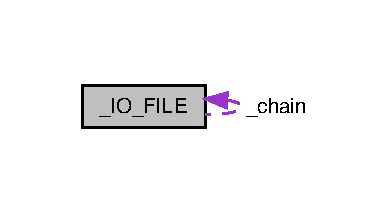
\includegraphics[width=187pt]{struct__IO__FILE__coll__graph}
\end{center}
\end{figure}
\subsection*{Champs de données}
\begin{DoxyCompactItemize}
\item 
int \hyperlink{struct__IO__FILE_a364ce3577f2cdb788df3a2a54909f45a}{\-\_\-flags}
\item 
char $\ast$ \hyperlink{struct__IO__FILE_a1c2f65148a6f2e35c478af0fc144fded}{\-\_\-\-I\-O\-\_\-read\-\_\-ptr}
\item 
char $\ast$ \hyperlink{struct__IO__FILE_a6994a0f73699af311e4669b4baa0e26b}{\-\_\-\-I\-O\-\_\-read\-\_\-end}
\item 
char $\ast$ \hyperlink{struct__IO__FILE_a2a449978f6e6aa2172f7f82ed1d42f37}{\-\_\-\-I\-O\-\_\-read\-\_\-base}
\item 
char $\ast$ \hyperlink{struct__IO__FILE_a6631dc1b00cd5a378280606c9333f40a}{\-\_\-\-I\-O\-\_\-write\-\_\-base}
\item 
char $\ast$ \hyperlink{struct__IO__FILE_ab746b60c0613c28d3451b13afdd703b5}{\-\_\-\-I\-O\-\_\-write\-\_\-ptr}
\item 
char $\ast$ \hyperlink{struct__IO__FILE_ad68f27b22fb43ab7a50bdaa50dc7d725}{\-\_\-\-I\-O\-\_\-write\-\_\-end}
\item 
char $\ast$ \hyperlink{struct__IO__FILE_a2bf5a30fdc43564cf2e46d2cce8e82dd}{\-\_\-\-I\-O\-\_\-buf\-\_\-base}
\item 
char $\ast$ \hyperlink{struct__IO__FILE_ac9fa3b261e95a246dac19dc35045be42}{\-\_\-\-I\-O\-\_\-buf\-\_\-end}
\item 
char $\ast$ \hyperlink{struct__IO__FILE_a3ef98bd6be88c72459cf4a670a5ba35c}{\-\_\-\-I\-O\-\_\-save\-\_\-base}
\item 
char $\ast$ \hyperlink{struct__IO__FILE_a8e6f38619f990a207a598132f4e6e661}{\-\_\-\-I\-O\-\_\-backup\-\_\-base}
\item 
char $\ast$ \hyperlink{struct__IO__FILE_a48102d534ea93a120fc025b1bead08cb}{\-\_\-\-I\-O\-\_\-save\-\_\-end}
\item 
\hypertarget{struct__IO__FILE_a148f6239f490808c7875a5d43f13e645}{struct \hyperlink{struct__IO__FILE}{\-\_\-\-I\-O\-\_\-\-F\-I\-L\-E} $\ast$ {\bfseries \-\_\-chain}}\label{struct__IO__FILE_a148f6239f490808c7875a5d43f13e645}

\item 
\hypertarget{struct__IO__FILE_a1883574299ff3f4ac644796985ca0a1d}{int {\bfseries \-\_\-fileno}}\label{struct__IO__FILE_a1883574299ff3f4ac644796985ca0a1d}

\end{DoxyCompactItemize}


\subsection{Documentation des champs}
\hypertarget{struct__IO__FILE_a364ce3577f2cdb788df3a2a54909f45a}{\index{\-\_\-\-I\-O\-\_\-\-F\-I\-L\-E@{\-\_\-\-I\-O\-\_\-\-F\-I\-L\-E}!\-\_\-flags@{\-\_\-flags}}
\index{\-\_\-flags@{\-\_\-flags}!_IO_FILE@{\-\_\-\-I\-O\-\_\-\-F\-I\-L\-E}}
\subsubsection[{\-\_\-flags}]{\setlength{\rightskip}{0pt plus 5cm}int \-\_\-\-I\-O\-\_\-\-F\-I\-L\-E\-::\-\_\-flags}}\label{struct__IO__FILE_a364ce3577f2cdb788df3a2a54909f45a}
High-\/order word is \-\_\-\-I\-O\-\_\-\-M\-A\-G\-I\-C; rest is flags. \hypertarget{struct__IO__FILE_a8e6f38619f990a207a598132f4e6e661}{\index{\-\_\-\-I\-O\-\_\-\-F\-I\-L\-E@{\-\_\-\-I\-O\-\_\-\-F\-I\-L\-E}!\-\_\-\-I\-O\-\_\-backup\-\_\-base@{\-\_\-\-I\-O\-\_\-backup\-\_\-base}}
\index{\-\_\-\-I\-O\-\_\-backup\-\_\-base@{\-\_\-\-I\-O\-\_\-backup\-\_\-base}!_IO_FILE@{\-\_\-\-I\-O\-\_\-\-F\-I\-L\-E}}
\subsubsection[{\-\_\-\-I\-O\-\_\-backup\-\_\-base}]{\setlength{\rightskip}{0pt plus 5cm}char$\ast$ \-\_\-\-I\-O\-\_\-\-F\-I\-L\-E\-::\-\_\-\-I\-O\-\_\-backup\-\_\-base}}\label{struct__IO__FILE_a8e6f38619f990a207a598132f4e6e661}
Pointer to first valid character of backup area \hypertarget{struct__IO__FILE_a2bf5a30fdc43564cf2e46d2cce8e82dd}{\index{\-\_\-\-I\-O\-\_\-\-F\-I\-L\-E@{\-\_\-\-I\-O\-\_\-\-F\-I\-L\-E}!\-\_\-\-I\-O\-\_\-buf\-\_\-base@{\-\_\-\-I\-O\-\_\-buf\-\_\-base}}
\index{\-\_\-\-I\-O\-\_\-buf\-\_\-base@{\-\_\-\-I\-O\-\_\-buf\-\_\-base}!_IO_FILE@{\-\_\-\-I\-O\-\_\-\-F\-I\-L\-E}}
\subsubsection[{\-\_\-\-I\-O\-\_\-buf\-\_\-base}]{\setlength{\rightskip}{0pt plus 5cm}char$\ast$ \-\_\-\-I\-O\-\_\-\-F\-I\-L\-E\-::\-\_\-\-I\-O\-\_\-buf\-\_\-base}}\label{struct__IO__FILE_a2bf5a30fdc43564cf2e46d2cce8e82dd}
Start of reserve area. \hypertarget{struct__IO__FILE_ac9fa3b261e95a246dac19dc35045be42}{\index{\-\_\-\-I\-O\-\_\-\-F\-I\-L\-E@{\-\_\-\-I\-O\-\_\-\-F\-I\-L\-E}!\-\_\-\-I\-O\-\_\-buf\-\_\-end@{\-\_\-\-I\-O\-\_\-buf\-\_\-end}}
\index{\-\_\-\-I\-O\-\_\-buf\-\_\-end@{\-\_\-\-I\-O\-\_\-buf\-\_\-end}!_IO_FILE@{\-\_\-\-I\-O\-\_\-\-F\-I\-L\-E}}
\subsubsection[{\-\_\-\-I\-O\-\_\-buf\-\_\-end}]{\setlength{\rightskip}{0pt plus 5cm}char$\ast$ \-\_\-\-I\-O\-\_\-\-F\-I\-L\-E\-::\-\_\-\-I\-O\-\_\-buf\-\_\-end}}\label{struct__IO__FILE_ac9fa3b261e95a246dac19dc35045be42}
End of reserve area. \hypertarget{struct__IO__FILE_a2a449978f6e6aa2172f7f82ed1d42f37}{\index{\-\_\-\-I\-O\-\_\-\-F\-I\-L\-E@{\-\_\-\-I\-O\-\_\-\-F\-I\-L\-E}!\-\_\-\-I\-O\-\_\-read\-\_\-base@{\-\_\-\-I\-O\-\_\-read\-\_\-base}}
\index{\-\_\-\-I\-O\-\_\-read\-\_\-base@{\-\_\-\-I\-O\-\_\-read\-\_\-base}!_IO_FILE@{\-\_\-\-I\-O\-\_\-\-F\-I\-L\-E}}
\subsubsection[{\-\_\-\-I\-O\-\_\-read\-\_\-base}]{\setlength{\rightskip}{0pt plus 5cm}char$\ast$ \-\_\-\-I\-O\-\_\-\-F\-I\-L\-E\-::\-\_\-\-I\-O\-\_\-read\-\_\-base}}\label{struct__IO__FILE_a2a449978f6e6aa2172f7f82ed1d42f37}
Start of putback+get area. \hypertarget{struct__IO__FILE_a6994a0f73699af311e4669b4baa0e26b}{\index{\-\_\-\-I\-O\-\_\-\-F\-I\-L\-E@{\-\_\-\-I\-O\-\_\-\-F\-I\-L\-E}!\-\_\-\-I\-O\-\_\-read\-\_\-end@{\-\_\-\-I\-O\-\_\-read\-\_\-end}}
\index{\-\_\-\-I\-O\-\_\-read\-\_\-end@{\-\_\-\-I\-O\-\_\-read\-\_\-end}!_IO_FILE@{\-\_\-\-I\-O\-\_\-\-F\-I\-L\-E}}
\subsubsection[{\-\_\-\-I\-O\-\_\-read\-\_\-end}]{\setlength{\rightskip}{0pt plus 5cm}char$\ast$ \-\_\-\-I\-O\-\_\-\-F\-I\-L\-E\-::\-\_\-\-I\-O\-\_\-read\-\_\-end}}\label{struct__IO__FILE_a6994a0f73699af311e4669b4baa0e26b}
End of get area. \hypertarget{struct__IO__FILE_a1c2f65148a6f2e35c478af0fc144fded}{\index{\-\_\-\-I\-O\-\_\-\-F\-I\-L\-E@{\-\_\-\-I\-O\-\_\-\-F\-I\-L\-E}!\-\_\-\-I\-O\-\_\-read\-\_\-ptr@{\-\_\-\-I\-O\-\_\-read\-\_\-ptr}}
\index{\-\_\-\-I\-O\-\_\-read\-\_\-ptr@{\-\_\-\-I\-O\-\_\-read\-\_\-ptr}!_IO_FILE@{\-\_\-\-I\-O\-\_\-\-F\-I\-L\-E}}
\subsubsection[{\-\_\-\-I\-O\-\_\-read\-\_\-ptr}]{\setlength{\rightskip}{0pt plus 5cm}char$\ast$ \-\_\-\-I\-O\-\_\-\-F\-I\-L\-E\-::\-\_\-\-I\-O\-\_\-read\-\_\-ptr}}\label{struct__IO__FILE_a1c2f65148a6f2e35c478af0fc144fded}
Current read pointer \hypertarget{struct__IO__FILE_a3ef98bd6be88c72459cf4a670a5ba35c}{\index{\-\_\-\-I\-O\-\_\-\-F\-I\-L\-E@{\-\_\-\-I\-O\-\_\-\-F\-I\-L\-E}!\-\_\-\-I\-O\-\_\-save\-\_\-base@{\-\_\-\-I\-O\-\_\-save\-\_\-base}}
\index{\-\_\-\-I\-O\-\_\-save\-\_\-base@{\-\_\-\-I\-O\-\_\-save\-\_\-base}!_IO_FILE@{\-\_\-\-I\-O\-\_\-\-F\-I\-L\-E}}
\subsubsection[{\-\_\-\-I\-O\-\_\-save\-\_\-base}]{\setlength{\rightskip}{0pt plus 5cm}char$\ast$ \-\_\-\-I\-O\-\_\-\-F\-I\-L\-E\-::\-\_\-\-I\-O\-\_\-save\-\_\-base}}\label{struct__IO__FILE_a3ef98bd6be88c72459cf4a670a5ba35c}
Pointer to start of non-\/current get area. \hypertarget{struct__IO__FILE_a48102d534ea93a120fc025b1bead08cb}{\index{\-\_\-\-I\-O\-\_\-\-F\-I\-L\-E@{\-\_\-\-I\-O\-\_\-\-F\-I\-L\-E}!\-\_\-\-I\-O\-\_\-save\-\_\-end@{\-\_\-\-I\-O\-\_\-save\-\_\-end}}
\index{\-\_\-\-I\-O\-\_\-save\-\_\-end@{\-\_\-\-I\-O\-\_\-save\-\_\-end}!_IO_FILE@{\-\_\-\-I\-O\-\_\-\-F\-I\-L\-E}}
\subsubsection[{\-\_\-\-I\-O\-\_\-save\-\_\-end}]{\setlength{\rightskip}{0pt plus 5cm}char$\ast$ \-\_\-\-I\-O\-\_\-\-F\-I\-L\-E\-::\-\_\-\-I\-O\-\_\-save\-\_\-end}}\label{struct__IO__FILE_a48102d534ea93a120fc025b1bead08cb}
Pointer to end of non-\/current get area. \hypertarget{struct__IO__FILE_a6631dc1b00cd5a378280606c9333f40a}{\index{\-\_\-\-I\-O\-\_\-\-F\-I\-L\-E@{\-\_\-\-I\-O\-\_\-\-F\-I\-L\-E}!\-\_\-\-I\-O\-\_\-write\-\_\-base@{\-\_\-\-I\-O\-\_\-write\-\_\-base}}
\index{\-\_\-\-I\-O\-\_\-write\-\_\-base@{\-\_\-\-I\-O\-\_\-write\-\_\-base}!_IO_FILE@{\-\_\-\-I\-O\-\_\-\-F\-I\-L\-E}}
\subsubsection[{\-\_\-\-I\-O\-\_\-write\-\_\-base}]{\setlength{\rightskip}{0pt plus 5cm}char$\ast$ \-\_\-\-I\-O\-\_\-\-F\-I\-L\-E\-::\-\_\-\-I\-O\-\_\-write\-\_\-base}}\label{struct__IO__FILE_a6631dc1b00cd5a378280606c9333f40a}
Start of put area. \hypertarget{struct__IO__FILE_ad68f27b22fb43ab7a50bdaa50dc7d725}{\index{\-\_\-\-I\-O\-\_\-\-F\-I\-L\-E@{\-\_\-\-I\-O\-\_\-\-F\-I\-L\-E}!\-\_\-\-I\-O\-\_\-write\-\_\-end@{\-\_\-\-I\-O\-\_\-write\-\_\-end}}
\index{\-\_\-\-I\-O\-\_\-write\-\_\-end@{\-\_\-\-I\-O\-\_\-write\-\_\-end}!_IO_FILE@{\-\_\-\-I\-O\-\_\-\-F\-I\-L\-E}}
\subsubsection[{\-\_\-\-I\-O\-\_\-write\-\_\-end}]{\setlength{\rightskip}{0pt plus 5cm}char$\ast$ \-\_\-\-I\-O\-\_\-\-F\-I\-L\-E\-::\-\_\-\-I\-O\-\_\-write\-\_\-end}}\label{struct__IO__FILE_ad68f27b22fb43ab7a50bdaa50dc7d725}
End of put area. \hypertarget{struct__IO__FILE_ab746b60c0613c28d3451b13afdd703b5}{\index{\-\_\-\-I\-O\-\_\-\-F\-I\-L\-E@{\-\_\-\-I\-O\-\_\-\-F\-I\-L\-E}!\-\_\-\-I\-O\-\_\-write\-\_\-ptr@{\-\_\-\-I\-O\-\_\-write\-\_\-ptr}}
\index{\-\_\-\-I\-O\-\_\-write\-\_\-ptr@{\-\_\-\-I\-O\-\_\-write\-\_\-ptr}!_IO_FILE@{\-\_\-\-I\-O\-\_\-\-F\-I\-L\-E}}
\subsubsection[{\-\_\-\-I\-O\-\_\-write\-\_\-ptr}]{\setlength{\rightskip}{0pt plus 5cm}char$\ast$ \-\_\-\-I\-O\-\_\-\-F\-I\-L\-E\-::\-\_\-\-I\-O\-\_\-write\-\_\-ptr}}\label{struct__IO__FILE_ab746b60c0613c28d3451b13afdd703b5}
Current put pointer. 

La documentation de cette structure a été générée à partir du fichier suivant \-:\begin{DoxyCompactItemize}
\item 
libc/include/\hyperlink{libio_8h}{libio.\-h}\end{DoxyCompactItemize}

\hypertarget{structdirent}{\section{Référence de la structure dirent}
\label{structdirent}\index{dirent@{dirent}}
}


{\ttfamily \#include $<$dirent.\-h$>$}

\subsection*{Champs de données}
\begin{DoxyCompactItemize}
\item 
\hyperlink{types_8h_a33594304e786b158f3fb30289278f5af}{uint32\-\_\-t} \hyperlink{structdirent_a0ed2e5ea3c71500f628914bf3966e4ba}{d\-\_\-ino}
\item 
\hyperlink{types_8h_adf4d876453337156dde61095e1f20223}{uint16\-\_\-t} \hyperlink{structdirent_a7cc67dd4ba5a8bed7f107f249957688d}{d\-\_\-reclen}
\item 
\hyperlink{types_8h_aba7bc1797add20fe3efdf37ced1182c5}{uint8\-\_\-t} \hyperlink{structdirent_a948760e3b7f607213a19f85e7af15a32}{d\-\_\-type}
\item 
char \hyperlink{structdirent_a7b4cbd53dc600257b2746225c8a8f3be}{d\-\_\-name} \mbox{[}\hyperlink{dirent_8h_ac64541bdd81c961304b9babef1402640}{N\-A\-M\-E\-\_\-\-M\-A\-X}\mbox{]}
\end{DoxyCompactItemize}


\subsection{Description détaillée}
Directory entry. 

\subsection{Documentation des champs}
\hypertarget{structdirent_a0ed2e5ea3c71500f628914bf3966e4ba}{\index{dirent@{dirent}!d\-\_\-ino@{d\-\_\-ino}}
\index{d\-\_\-ino@{d\-\_\-ino}!dirent@{dirent}}
\subsubsection[{d\-\_\-ino}]{\setlength{\rightskip}{0pt plus 5cm}{\bf uint32\-\_\-t} dirent\-::d\-\_\-ino}}\label{structdirent_a0ed2e5ea3c71500f628914bf3966e4ba}
Numéro inode. \hypertarget{structdirent_a7b4cbd53dc600257b2746225c8a8f3be}{\index{dirent@{dirent}!d\-\_\-name@{d\-\_\-name}}
\index{d\-\_\-name@{d\-\_\-name}!dirent@{dirent}}
\subsubsection[{d\-\_\-name}]{\setlength{\rightskip}{0pt plus 5cm}char dirent\-::d\-\_\-name\mbox{[}{\bf N\-A\-M\-E\-\_\-\-M\-A\-X}\mbox{]}}}\label{structdirent_a7b4cbd53dc600257b2746225c8a8f3be}
Nom du fichier. \hypertarget{structdirent_a7cc67dd4ba5a8bed7f107f249957688d}{\index{dirent@{dirent}!d\-\_\-reclen@{d\-\_\-reclen}}
\index{d\-\_\-reclen@{d\-\_\-reclen}!dirent@{dirent}}
\subsubsection[{d\-\_\-reclen}]{\setlength{\rightskip}{0pt plus 5cm}{\bf uint16\-\_\-t} dirent\-::d\-\_\-reclen}}\label{structdirent_a7cc67dd4ba5a8bed7f107f249957688d}
Taille de l'entrée. \hypertarget{structdirent_a948760e3b7f607213a19f85e7af15a32}{\index{dirent@{dirent}!d\-\_\-type@{d\-\_\-type}}
\index{d\-\_\-type@{d\-\_\-type}!dirent@{dirent}}
\subsubsection[{d\-\_\-type}]{\setlength{\rightskip}{0pt plus 5cm}{\bf uint8\-\_\-t} dirent\-::d\-\_\-type}}\label{structdirent_a948760e3b7f607213a19f85e7af15a32}
Type de fichier. 

La documentation de cette structure a été générée à partir du fichier suivant \-:\begin{DoxyCompactItemize}
\item 
libc/include/\hyperlink{dirent_8h}{dirent.\-h}\end{DoxyCompactItemize}

\hypertarget{structmem}{\section{\-Référence de la structure mem}
\label{structmem}\index{mem@{mem}}
}


\-Graphe de collaboration de mem\-:\nopagebreak
\begin{figure}[H]
\begin{center}
\leavevmode
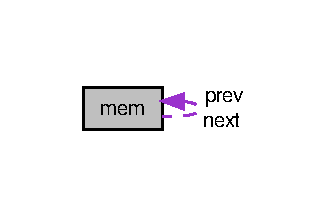
\includegraphics[width=158pt]{structmem__coll__graph}
\end{center}
\end{figure}
\subsection*{\-Champs de données}
\begin{DoxyCompactItemize}
\item 
\hypertarget{structmem_a2edfcacfe26d9112b0e4f745c9f75cf7}{struct \hyperlink{structmem}{mem} $\ast$ {\bfseries prev}}\label{structmem_a2edfcacfe26d9112b0e4f745c9f75cf7}

\item 
\hypertarget{structmem_a7d695ebc3fafa769e7e7a75f1d232a18}{\hyperlink{types_8h_a29d85914ddff32967d85ada69854206d}{size\-\_\-t} {\bfseries size}}\label{structmem_a7d695ebc3fafa769e7e7a75f1d232a18}

\item 
\hypertarget{structmem_ad12075ee870ccc6f67f420f09ff37732}{struct \hyperlink{structmem}{mem} $\ast$ {\bfseries next}}\label{structmem_ad12075ee870ccc6f67f420f09ff37732}

\end{DoxyCompactItemize}


\-La documentation de cette structure a été générée à partir du fichier suivant \-:\begin{DoxyCompactItemize}
\item 
libc/\hyperlink{malloc_8c}{malloc.\-c}\end{DoxyCompactItemize}

\hypertarget{structmem__list}{\section{Référence de la structure mem\-\_\-list}
\label{structmem__list}\index{mem\-\_\-list@{mem\-\_\-list}}
}


Graphe de collaboration de mem\-\_\-list\-:\nopagebreak
\begin{figure}[H]
\begin{center}
\leavevmode
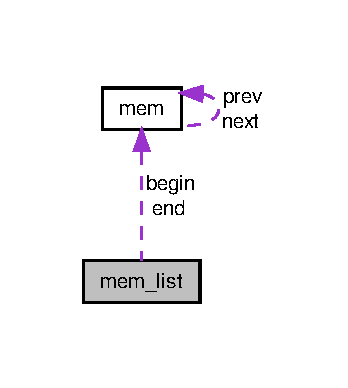
\includegraphics[width=167pt]{structmem__list__coll__graph}
\end{center}
\end{figure}
\subsection*{Champs de données}
\begin{DoxyCompactItemize}
\item 
\hypertarget{structmem__list_a553c3121bc3eb64cb30d5cda16edb629}{struct \hyperlink{structmem}{mem} $\ast$ {\bfseries begin}}\label{structmem__list_a553c3121bc3eb64cb30d5cda16edb629}

\item 
\hypertarget{structmem__list_a2e221a43fa8f185dda7f582fbb4c507f}{struct \hyperlink{structmem}{mem} $\ast$ {\bfseries end}}\label{structmem__list_a2e221a43fa8f185dda7f582fbb4c507f}

\end{DoxyCompactItemize}


La documentation de cette structure a été générée à partir du fichier suivant \-:\begin{DoxyCompactItemize}
\item 
kernel/\hyperlink{kmalloc_8c}{kmalloc.\-c}\end{DoxyCompactItemize}

\hypertarget{structstat}{\section{Référence de la structure stat}
\label{structstat}\index{stat@{stat}}
}


Informations sur un noeud.  




{\ttfamily \#include $<$kstat.\-h$>$}

\subsection*{Champs de données}
\begin{DoxyCompactItemize}
\item 
\hyperlink{kstat_8h_a451f1b5788fa7cc5d33db47a5992e7a6}{dev\-\_\-t} \hyperlink{structstat_ac5b90090ae323741ae4c9e4f3683a29f}{st\-\_\-dev}
\item 
\hyperlink{kstat_8h_aed4e918b44240739869c4bdb1c4787a9}{ino\-\_\-t} \hyperlink{structstat_a9769ed8f0d4c5a9f329c32bc92479d56}{st\-\_\-ino}
\item 
\hyperlink{kstat_8h_af8f4385bb42836d1e3ad4fea9d71d1b9}{mode\-\_\-t} \hyperlink{structstat_a5cbdd829011af82ba61e83773bbcbc7d}{st\-\_\-mode}
\item 
nlink\-\_\-t \hyperlink{structstat_a0ed9092fa6c77a3251b9b9a4738ef84f}{st\-\_\-nlink}
\item 
\hyperlink{kstat_8h_af2306308627701b66dc6f3babe821ab4}{uid\-\_\-t} \hyperlink{structstat_a4a8708a3d18be60ee7b2f06c4cab0c70}{st\-\_\-uid}
\item 
\hyperlink{kstat_8h_aa7352f1065fe606194d792e2b292cf83}{gid\-\_\-t} \hyperlink{structstat_ab864f16f436cec370f0ced585d897698}{st\-\_\-gid}
\item 
\hyperlink{kstat_8h_a451f1b5788fa7cc5d33db47a5992e7a6}{dev\-\_\-t} \hyperlink{structstat_aa61e6c1a8a91c69f1d26f6700a0546cb}{st\-\_\-rdev}
\item 
\hyperlink{libc_2include_2sys_2types_8h_a447a6a64dbb8fb44b1e62856b333db4a}{off\-\_\-t} \hyperlink{structstat_a040e19c8b9766f841fde8786ce9297bf}{st\-\_\-size}
\item 
blksize\-\_\-t \hyperlink{structstat_a38d474e1ae3cf6fbdde89ac3c3e308f1}{st\-\_\-blksize}
\item 
blkcnt\-\_\-t \hyperlink{structstat_a42dd716b2f9234f961d949fc9500eefb}{st\-\_\-blocks}
\item 
\hyperlink{time_8h_aaaf414ca0598a3633e6e9161cbb5a58a}{time\-\_\-t} \hyperlink{structstat_ab74d1e7e345e88b9d0fb2688a97cba64}{st\-\_\-atime}
\item 
\hyperlink{time_8h_aaaf414ca0598a3633e6e9161cbb5a58a}{time\-\_\-t} \hyperlink{structstat_a77e235090f8cb6897f1c0ce65689006b}{st\-\_\-mtime}
\item 
\hyperlink{time_8h_aaaf414ca0598a3633e6e9161cbb5a58a}{time\-\_\-t} \hyperlink{structstat_a1b4b858db1ebe79c3d6e0fc1ef721024}{st\-\_\-ctime}
\end{DoxyCompactItemize}


\subsection{Description détaillée}
Structure contenant les informations d'un noeud. 

\subsection{Documentation des champs}
\hypertarget{structstat_ab74d1e7e345e88b9d0fb2688a97cba64}{\index{stat@{stat}!st\-\_\-atime@{st\-\_\-atime}}
\index{st\-\_\-atime@{st\-\_\-atime}!stat@{stat}}
\subsubsection[{st\-\_\-atime}]{\setlength{\rightskip}{0pt plus 5cm}{\bf time\-\_\-t} stat\-::st\-\_\-atime}}\label{structstat_ab74d1e7e345e88b9d0fb2688a97cba64}
Heure dernier accès \hypertarget{structstat_a38d474e1ae3cf6fbdde89ac3c3e308f1}{\index{stat@{stat}!st\-\_\-blksize@{st\-\_\-blksize}}
\index{st\-\_\-blksize@{st\-\_\-blksize}!stat@{stat}}
\subsubsection[{st\-\_\-blksize}]{\setlength{\rightskip}{0pt plus 5cm}blksize\-\_\-t stat\-::st\-\_\-blksize}}\label{structstat_a38d474e1ae3cf6fbdde89ac3c3e308f1}
Taille de bloc pour E/\-S \hypertarget{structstat_a42dd716b2f9234f961d949fc9500eefb}{\index{stat@{stat}!st\-\_\-blocks@{st\-\_\-blocks}}
\index{st\-\_\-blocks@{st\-\_\-blocks}!stat@{stat}}
\subsubsection[{st\-\_\-blocks}]{\setlength{\rightskip}{0pt plus 5cm}blkcnt\-\_\-t stat\-::st\-\_\-blocks}}\label{structstat_a42dd716b2f9234f961d949fc9500eefb}
Nombre de blocs de 512\-B alloués \hypertarget{structstat_a1b4b858db1ebe79c3d6e0fc1ef721024}{\index{stat@{stat}!st\-\_\-ctime@{st\-\_\-ctime}}
\index{st\-\_\-ctime@{st\-\_\-ctime}!stat@{stat}}
\subsubsection[{st\-\_\-ctime}]{\setlength{\rightskip}{0pt plus 5cm}{\bf time\-\_\-t} stat\-::st\-\_\-ctime}}\label{structstat_a1b4b858db1ebe79c3d6e0fc1ef721024}
Heure dernier changement état \hypertarget{structstat_ac5b90090ae323741ae4c9e4f3683a29f}{\index{stat@{stat}!st\-\_\-dev@{st\-\_\-dev}}
\index{st\-\_\-dev@{st\-\_\-dev}!stat@{stat}}
\subsubsection[{st\-\_\-dev}]{\setlength{\rightskip}{0pt plus 5cm}{\bf dev\-\_\-t} stat\-::st\-\_\-dev}}\label{structstat_ac5b90090ae323741ae4c9e4f3683a29f}
Périphérique \hypertarget{structstat_ab864f16f436cec370f0ced585d897698}{\index{stat@{stat}!st\-\_\-gid@{st\-\_\-gid}}
\index{st\-\_\-gid@{st\-\_\-gid}!stat@{stat}}
\subsubsection[{st\-\_\-gid}]{\setlength{\rightskip}{0pt plus 5cm}{\bf gid\-\_\-t} stat\-::st\-\_\-gid}}\label{structstat_ab864f16f436cec370f0ced585d897698}
G\-I\-D propriétaire \hypertarget{structstat_a9769ed8f0d4c5a9f329c32bc92479d56}{\index{stat@{stat}!st\-\_\-ino@{st\-\_\-ino}}
\index{st\-\_\-ino@{st\-\_\-ino}!stat@{stat}}
\subsubsection[{st\-\_\-ino}]{\setlength{\rightskip}{0pt plus 5cm}{\bf ino\-\_\-t} stat\-::st\-\_\-ino}}\label{structstat_a9769ed8f0d4c5a9f329c32bc92479d56}
Numéro inœud \hypertarget{structstat_a5cbdd829011af82ba61e83773bbcbc7d}{\index{stat@{stat}!st\-\_\-mode@{st\-\_\-mode}}
\index{st\-\_\-mode@{st\-\_\-mode}!stat@{stat}}
\subsubsection[{st\-\_\-mode}]{\setlength{\rightskip}{0pt plus 5cm}{\bf mode\-\_\-t} stat\-::st\-\_\-mode}}\label{structstat_a5cbdd829011af82ba61e83773bbcbc7d}
Protection + file type \hypertarget{structstat_a77e235090f8cb6897f1c0ce65689006b}{\index{stat@{stat}!st\-\_\-mtime@{st\-\_\-mtime}}
\index{st\-\_\-mtime@{st\-\_\-mtime}!stat@{stat}}
\subsubsection[{st\-\_\-mtime}]{\setlength{\rightskip}{0pt plus 5cm}{\bf time\-\_\-t} stat\-::st\-\_\-mtime}}\label{structstat_a77e235090f8cb6897f1c0ce65689006b}
Heure dernière modification \hypertarget{structstat_a0ed9092fa6c77a3251b9b9a4738ef84f}{\index{stat@{stat}!st\-\_\-nlink@{st\-\_\-nlink}}
\index{st\-\_\-nlink@{st\-\_\-nlink}!stat@{stat}}
\subsubsection[{st\-\_\-nlink}]{\setlength{\rightskip}{0pt plus 5cm}nlink\-\_\-t stat\-::st\-\_\-nlink}}\label{structstat_a0ed9092fa6c77a3251b9b9a4738ef84f}
Nb liens matériels \hypertarget{structstat_aa61e6c1a8a91c69f1d26f6700a0546cb}{\index{stat@{stat}!st\-\_\-rdev@{st\-\_\-rdev}}
\index{st\-\_\-rdev@{st\-\_\-rdev}!stat@{stat}}
\subsubsection[{st\-\_\-rdev}]{\setlength{\rightskip}{0pt plus 5cm}{\bf dev\-\_\-t} stat\-::st\-\_\-rdev}}\label{structstat_aa61e6c1a8a91c69f1d26f6700a0546cb}
Type périphérique \hypertarget{structstat_a040e19c8b9766f841fde8786ce9297bf}{\index{stat@{stat}!st\-\_\-size@{st\-\_\-size}}
\index{st\-\_\-size@{st\-\_\-size}!stat@{stat}}
\subsubsection[{st\-\_\-size}]{\setlength{\rightskip}{0pt plus 5cm}{\bf off\-\_\-t} stat\-::st\-\_\-size}}\label{structstat_a040e19c8b9766f841fde8786ce9297bf}
Taille totale en octets \hypertarget{structstat_a4a8708a3d18be60ee7b2f06c4cab0c70}{\index{stat@{stat}!st\-\_\-uid@{st\-\_\-uid}}
\index{st\-\_\-uid@{st\-\_\-uid}!stat@{stat}}
\subsubsection[{st\-\_\-uid}]{\setlength{\rightskip}{0pt plus 5cm}{\bf uid\-\_\-t} stat\-::st\-\_\-uid}}\label{structstat_a4a8708a3d18be60ee7b2f06c4cab0c70}
U\-I\-D propriétaire 

La documentation de cette structure a été générée à partir des fichiers suivants \-:\begin{DoxyCompactItemize}
\item 
kernel/include/\hyperlink{kstat_8h}{kstat.\-h}\item 
libc/include/sys/\hyperlink{stat_8h}{stat.\-h}\end{DoxyCompactItemize}

\hypertarget{structtermios}{\section{Référence de la structure termios}
\label{structtermios}\index{termios@{termios}}
}
\subsection*{Champs de données}
\begin{DoxyCompactItemize}
\item 
tcflag\-\_\-t \hyperlink{structtermios_a85b6c86d2a3db45a3829488190e357e4}{c\-\_\-iflag}
\item 
tcflag\-\_\-t \hyperlink{structtermios_ad6e2cfedb81530e5a6a3a0e30b8c6362}{c\-\_\-oflag}
\item 
tcflag\-\_\-t \hyperlink{structtermios_a5d42b95faa4745c3bea53652d2812162}{c\-\_\-cflag}
\item 
tcflag\-\_\-t \hyperlink{structtermios_a91bdd7691180800fccc4b791466ee9c3}{c\-\_\-lflag}
\item 
cc\-\_\-t \hyperlink{structtermios_a6058cfc222551ee750c72142299acb2e}{c\-\_\-cc} \mbox{[}N\-C\-C\-S\mbox{]}
\item 
speed\-\_\-t \hyperlink{structtermios_a02ae972cbc9fb2cf4a1aa6a6751a421a}{c\-\_\-ispeed}
\end{DoxyCompactItemize}


\subsection{Documentation des champs}
\hypertarget{structtermios_a6058cfc222551ee750c72142299acb2e}{\index{termios@{termios}!c\-\_\-cc@{c\-\_\-cc}}
\index{c\-\_\-cc@{c\-\_\-cc}!termios@{termios}}
\subsubsection[{c\-\_\-cc}]{\setlength{\rightskip}{0pt plus 5cm}cc\-\_\-t termios\-::c\-\_\-cc}}\label{structtermios_a6058cfc222551ee750c72142299acb2e}
Control chars. \hypertarget{structtermios_a5d42b95faa4745c3bea53652d2812162}{\index{termios@{termios}!c\-\_\-cflag@{c\-\_\-cflag}}
\index{c\-\_\-cflag@{c\-\_\-cflag}!termios@{termios}}
\subsubsection[{c\-\_\-cflag}]{\setlength{\rightskip}{0pt plus 5cm}tcflag\-\_\-t termios\-::c\-\_\-cflag}}\label{structtermios_a5d42b95faa4745c3bea53652d2812162}
Control modes. \hypertarget{structtermios_a85b6c86d2a3db45a3829488190e357e4}{\index{termios@{termios}!c\-\_\-iflag@{c\-\_\-iflag}}
\index{c\-\_\-iflag@{c\-\_\-iflag}!termios@{termios}}
\subsubsection[{c\-\_\-iflag}]{\setlength{\rightskip}{0pt plus 5cm}tcflag\-\_\-t termios\-::c\-\_\-iflag}}\label{structtermios_a85b6c86d2a3db45a3829488190e357e4}
Input modes. \hypertarget{structtermios_a02ae972cbc9fb2cf4a1aa6a6751a421a}{\index{termios@{termios}!c\-\_\-ispeed@{c\-\_\-ispeed}}
\index{c\-\_\-ispeed@{c\-\_\-ispeed}!termios@{termios}}
\subsubsection[{c\-\_\-ispeed}]{\setlength{\rightskip}{0pt plus 5cm}speed\-\_\-t termios\-::c\-\_\-ispeed}}\label{structtermios_a02ae972cbc9fb2cf4a1aa6a6751a421a}
Speed (serial). \hypertarget{structtermios_a91bdd7691180800fccc4b791466ee9c3}{\index{termios@{termios}!c\-\_\-lflag@{c\-\_\-lflag}}
\index{c\-\_\-lflag@{c\-\_\-lflag}!termios@{termios}}
\subsubsection[{c\-\_\-lflag}]{\setlength{\rightskip}{0pt plus 5cm}tcflag\-\_\-t termios\-::c\-\_\-lflag}}\label{structtermios_a91bdd7691180800fccc4b791466ee9c3}
Local modes. \hypertarget{structtermios_ad6e2cfedb81530e5a6a3a0e30b8c6362}{\index{termios@{termios}!c\-\_\-oflag@{c\-\_\-oflag}}
\index{c\-\_\-oflag@{c\-\_\-oflag}!termios@{termios}}
\subsubsection[{c\-\_\-oflag}]{\setlength{\rightskip}{0pt plus 5cm}tcflag\-\_\-t termios\-::c\-\_\-oflag}}\label{structtermios_ad6e2cfedb81530e5a6a3a0e30b8c6362}
Output modes. 

La documentation de cette structure a été générée à partir des fichiers suivants \-:\begin{DoxyCompactItemize}
\item 
kernel/include/\hyperlink{termios__types_8h}{termios\-\_\-types.\-h}\item 
libc/include/\hyperlink{termios_8h}{termios.\-h}\end{DoxyCompactItemize}

\hypertarget{structtimespec}{\section{Référence de la structure timespec}
\label{structtimespec}\index{timespec@{timespec}}
}


{\ttfamily \#include $<$clock.\-h$>$}

\subsection*{Champs de données}
\begin{DoxyCompactItemize}
\item 
long int \hyperlink{structtimespec_af632894a12c37dea87073c0126f99fff}{tv\-\_\-sec}
\item 
long int \hyperlink{structtimespec_aa9689622a344d847333e534ac23d3093}{tv\-\_\-nsec}
\end{DoxyCompactItemize}


\subsection{Description détaillée}
Représente un temps écoule. 

\subsection{Documentation des champs}
\hypertarget{structtimespec_aa9689622a344d847333e534ac23d3093}{\index{timespec@{timespec}!tv\-\_\-nsec@{tv\-\_\-nsec}}
\index{tv\-\_\-nsec@{tv\-\_\-nsec}!timespec@{timespec}}
\subsubsection[{tv\-\_\-nsec}]{\setlength{\rightskip}{0pt plus 5cm}long int timespec\-::tv\-\_\-nsec}}\label{structtimespec_aa9689622a344d847333e534ac23d3093}
Le reste en ns. \hypertarget{structtimespec_af632894a12c37dea87073c0126f99fff}{\index{timespec@{timespec}!tv\-\_\-sec@{tv\-\_\-sec}}
\index{tv\-\_\-sec@{tv\-\_\-sec}!timespec@{timespec}}
\subsubsection[{tv\-\_\-sec}]{\setlength{\rightskip}{0pt plus 5cm}long int timespec\-::tv\-\_\-sec}}\label{structtimespec_af632894a12c37dea87073c0126f99fff}
Le nombre de secondes écoulées. 

La documentation de cette structure a été générée à partir du fichier suivant \-:\begin{DoxyCompactItemize}
\item 
kernel/include/\hyperlink{clock_8h}{clock.\-h}\end{DoxyCompactItemize}

\hypertarget{structtimeval}{\section{\-Référence de la structure timeval}
\label{structtimeval}\index{timeval@{timeval}}
}
\subsection*{\-Champs de données}
\begin{DoxyCompactItemize}
\item 
long int \hyperlink{structtimeval_ab6fac84a084d017bb157f4681dafe8a3}{tv\-\_\-sec}
\item 
long int \hyperlink{structtimeval_a6f90a236deb00a89fe3dd8023d525d9c}{tv\-\_\-usec}
\end{DoxyCompactItemize}


\subsection{\-Documentation des champs}
\hypertarget{structtimeval_ab6fac84a084d017bb157f4681dafe8a3}{\index{timeval@{timeval}!tv\-\_\-sec@{tv\-\_\-sec}}
\index{tv\-\_\-sec@{tv\-\_\-sec}!timeval@{timeval}}
\subsubsection[{tv\-\_\-sec}]{\setlength{\rightskip}{0pt plus 5cm}long int {\bf timeval\-::tv\-\_\-sec}}}\label{structtimeval_ab6fac84a084d017bb157f4681dafe8a3}
\-Secondes \hypertarget{structtimeval_a6f90a236deb00a89fe3dd8023d525d9c}{\index{timeval@{timeval}!tv\-\_\-usec@{tv\-\_\-usec}}
\index{tv\-\_\-usec@{tv\-\_\-usec}!timeval@{timeval}}
\subsubsection[{tv\-\_\-usec}]{\setlength{\rightskip}{0pt plus 5cm}long int {\bf timeval\-::tv\-\_\-usec}}}\label{structtimeval_a6f90a236deb00a89fe3dd8023d525d9c}
\-Microsecondes 

\-La documentation de cette structure a été générée à partir du fichier suivant \-:\begin{DoxyCompactItemize}
\item 
libc/include/\hyperlink{time_8h}{time.\-h}\end{DoxyCompactItemize}

\hypertarget{structtm}{\section{Référence de la structure tm}
\label{structtm}\index{tm@{tm}}
}


{\ttfamily \#include $<$clock.\+h$>$}

\subsection*{Champs de données}
\begin{DoxyCompactItemize}
\item 
int \hyperlink{structtm_a4d098a9a5c03a00b2ee61e10851de81e}{tm\+\_\+sec}
\item 
int \hyperlink{structtm_af414eb7c86cc3099595211eee4d4211b}{tm\+\_\+min}
\item 
int \hyperlink{structtm_a3e7ca4e37f1abcaf56b8a916c38eb9fe}{tm\+\_\+hour}
\item 
int \hyperlink{structtm_ab8d8904bad43b0c8b96e61941c5b5310}{tm\+\_\+mday}
\item 
int \hyperlink{structtm_a112ac36fa2f593777138a417cf031e17}{tm\+\_\+mon}
\item 
int \hyperlink{structtm_a33adf78fd6476b2120ce3b9c4a852053}{tm\+\_\+year}
\item 
int \hyperlink{structtm_afe81a8c46f1c693c43f259b288859f4f}{tm\+\_\+wday}
\item 
int \hyperlink{structtm_a93a0ba77cc23796df84405dcbcc57eb1}{tm\+\_\+yday}
\item 
int \hyperlink{structtm_a5645ca0580c8ab2c24f6c2965d9c9f9c}{tm\+\_\+isdst}
\end{DoxyCompactItemize}


\subsection{Description détaillée}
Structure qui contient une date et heure. 

\subsection{Documentation des champs}
\hypertarget{structtm_a3e7ca4e37f1abcaf56b8a916c38eb9fe}{\index{tm@{tm}!tm\+\_\+hour@{tm\+\_\+hour}}
\index{tm\+\_\+hour@{tm\+\_\+hour}!tm@{tm}}
\subsubsection[{tm\+\_\+hour}]{\setlength{\rightskip}{0pt plus 5cm}int tm\+::tm\+\_\+hour}}\label{structtm_a3e7ca4e37f1abcaf56b8a916c38eb9fe}
hours since midnight — \mbox{[}0, 23\mbox{]} \hypertarget{structtm_a5645ca0580c8ab2c24f6c2965d9c9f9c}{\index{tm@{tm}!tm\+\_\+isdst@{tm\+\_\+isdst}}
\index{tm\+\_\+isdst@{tm\+\_\+isdst}!tm@{tm}}
\subsubsection[{tm\+\_\+isdst}]{\setlength{\rightskip}{0pt plus 5cm}int tm\+::tm\+\_\+isdst}}\label{structtm_a5645ca0580c8ab2c24f6c2965d9c9f9c}
Daylight Saving Time flag (1 true, 0 false, neg unavailable) \hypertarget{structtm_ab8d8904bad43b0c8b96e61941c5b5310}{\index{tm@{tm}!tm\+\_\+mday@{tm\+\_\+mday}}
\index{tm\+\_\+mday@{tm\+\_\+mday}!tm@{tm}}
\subsubsection[{tm\+\_\+mday}]{\setlength{\rightskip}{0pt plus 5cm}int tm\+::tm\+\_\+mday}}\label{structtm_ab8d8904bad43b0c8b96e61941c5b5310}
day of the month — \mbox{[}1, 31\mbox{]} \hypertarget{structtm_af414eb7c86cc3099595211eee4d4211b}{\index{tm@{tm}!tm\+\_\+min@{tm\+\_\+min}}
\index{tm\+\_\+min@{tm\+\_\+min}!tm@{tm}}
\subsubsection[{tm\+\_\+min}]{\setlength{\rightskip}{0pt plus 5cm}int tm\+::tm\+\_\+min}}\label{structtm_af414eb7c86cc3099595211eee4d4211b}
minutes after the hour — \mbox{[}0, 59\mbox{]} \hypertarget{structtm_a112ac36fa2f593777138a417cf031e17}{\index{tm@{tm}!tm\+\_\+mon@{tm\+\_\+mon}}
\index{tm\+\_\+mon@{tm\+\_\+mon}!tm@{tm}}
\subsubsection[{tm\+\_\+mon}]{\setlength{\rightskip}{0pt plus 5cm}int tm\+::tm\+\_\+mon}}\label{structtm_a112ac36fa2f593777138a417cf031e17}
months since January — \mbox{[}0, 11\mbox{]} \hypertarget{structtm_a4d098a9a5c03a00b2ee61e10851de81e}{\index{tm@{tm}!tm\+\_\+sec@{tm\+\_\+sec}}
\index{tm\+\_\+sec@{tm\+\_\+sec}!tm@{tm}}
\subsubsection[{tm\+\_\+sec}]{\setlength{\rightskip}{0pt plus 5cm}int tm\+::tm\+\_\+sec}}\label{structtm_a4d098a9a5c03a00b2ee61e10851de81e}
seconds after the minute — \mbox{[}0, 60\mbox{]} \hypertarget{structtm_afe81a8c46f1c693c43f259b288859f4f}{\index{tm@{tm}!tm\+\_\+wday@{tm\+\_\+wday}}
\index{tm\+\_\+wday@{tm\+\_\+wday}!tm@{tm}}
\subsubsection[{tm\+\_\+wday}]{\setlength{\rightskip}{0pt plus 5cm}int tm\+::tm\+\_\+wday}}\label{structtm_afe81a8c46f1c693c43f259b288859f4f}
days since Sunday — \mbox{[}0, 6\mbox{]} \hypertarget{structtm_a93a0ba77cc23796df84405dcbcc57eb1}{\index{tm@{tm}!tm\+\_\+yday@{tm\+\_\+yday}}
\index{tm\+\_\+yday@{tm\+\_\+yday}!tm@{tm}}
\subsubsection[{tm\+\_\+yday}]{\setlength{\rightskip}{0pt plus 5cm}int tm\+::tm\+\_\+yday}}\label{structtm_a93a0ba77cc23796df84405dcbcc57eb1}
days since January 1 — \mbox{[}0, 365\mbox{]} \hypertarget{structtm_a33adf78fd6476b2120ce3b9c4a852053}{\index{tm@{tm}!tm\+\_\+year@{tm\+\_\+year}}
\index{tm\+\_\+year@{tm\+\_\+year}!tm@{tm}}
\subsubsection[{tm\+\_\+year}]{\setlength{\rightskip}{0pt plus 5cm}int tm\+::tm\+\_\+year}}\label{structtm_a33adf78fd6476b2120ce3b9c4a852053}
years since 1900 

La documentation de cette structure a été générée à partir des fichiers suivants \+:\begin{DoxyCompactItemize}
\item 
kernel/include/\hyperlink{clock_8h}{clock.\+h}\item 
libc/include/\hyperlink{time_8h}{time.\+h}\end{DoxyCompactItemize}

\hypertarget{structwinsize}{\section{\-Référence de la structure winsize}
\label{structwinsize}\index{winsize@{winsize}}
}
\subsection*{\-Champs de données}
\begin{DoxyCompactItemize}
\item 
\hypertarget{structwinsize_a73698fa1d966374b0701e4bf225f0141}{unsigned short {\bfseries ws\-\_\-row}}\label{structwinsize_a73698fa1d966374b0701e4bf225f0141}

\item 
\hypertarget{structwinsize_a80bedf71a49fd324e0d92d0702cc7005}{unsigned short {\bfseries ws\-\_\-col}}\label{structwinsize_a80bedf71a49fd324e0d92d0702cc7005}

\end{DoxyCompactItemize}


\-La documentation de cette structure a été générée à partir du fichier suivant \-:\begin{DoxyCompactItemize}
\item 
kernel/include/\hyperlink{tty_8h}{tty.\-h}\end{DoxyCompactItemize}

\chapter{Documentation des fichiers}
\hypertarget{ctype_8c}{\section{Référence du fichier libc/ctype.c}
\label{ctype_8c}\index{libc/ctype.\-c@{libc/ctype.\-c}}
}


Fonctions de classification des caractères.  


{\ttfamily \#include $<$ctype.\-h$>$}\\*
Graphe des dépendances par inclusion de ctype.\-c\-:\nopagebreak
\begin{figure}[H]
\begin{center}
\leavevmode
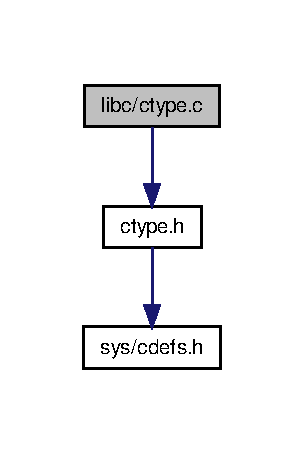
\includegraphics[width=144pt]{ctype_8c__incl}
\end{center}
\end{figure}
\subsection*{Fonctions}
\begin{DoxyCompactItemize}
\item 
int \hyperlink{ctype_8c_adf38e126f73a010f30af76db2a28c6e1}{isalnum} (int c)
\begin{DoxyCompactList}\small\item\em vérifie si l'on a un caractère alphanumérique. \end{DoxyCompactList}\item 
int \hyperlink{ctype_8c_a25908ae63aac2df990634e1ae5bd14d9}{isalpha} (int c)
\begin{DoxyCompactList}\small\item\em vérifie si l'on a un caractère alphabétique. \end{DoxyCompactList}\item 
int \hyperlink{ctype_8c_aea4929b1b41f1a6d723e0312b1f050ed}{isblank} (int c)
\begin{DoxyCompactList}\small\item\em vérifie si le caractère est blanc, c'est-\/à-\/dire un espace ou une tabulation. \end{DoxyCompactList}\item 
int \hyperlink{ctype_8c_a0008a4e8e7889734dc1d83297de07158}{iscntrl} (int c)
\begin{DoxyCompactList}\small\item\em vérifie si l'on a un caractère de contrôle. \end{DoxyCompactList}\item 
int \hyperlink{ctype_8c_a3fa45b35c8abf67a950b6d3d4063dede}{isdigit} (int c)
\begin{DoxyCompactList}\small\item\em vérifie si l'on a un chiffre (0 à 9). \end{DoxyCompactList}\item 
int \hyperlink{ctype_8c_a7b8f652a0423a80922dd89d8829db5f2}{islower} (int c)
\begin{DoxyCompactList}\small\item\em vérifie si l'on a un caractère minuscule. \end{DoxyCompactList}\item 
int \hyperlink{ctype_8c_a99355d8f0fb41ec43effb95189db0ed4}{isprint} (int c)
\begin{DoxyCompactList}\small\item\em vérifie s'il s'agit d'un caractère imprimable, y compris l'espace. \end{DoxyCompactList}\item 
int \hyperlink{ctype_8c_af29554b3ec04ea7684482bffed5dbce6}{ispunct} (int c)
\begin{DoxyCompactList}\small\item\em vérifie s'il s'agit d'un caractère imprimable, qui ne soit ni un espace, ni un caractère alphanumérique. \end{DoxyCompactList}\item 
int \hyperlink{ctype_8c_a56be4166e4673843042a548a7f513dbc}{isspace} (int c)
\begin{DoxyCompactList}\small\item\em vérifie si l'on a un caractère blanc, d'espacement. \end{DoxyCompactList}\item 
int \hyperlink{ctype_8c_adadd6582d46775aab6a51e29d16d9f77}{isupper} (int c)
\begin{DoxyCompactList}\small\item\em vérifie si l'on a un caractère majuscule. \end{DoxyCompactList}\item 
int \hyperlink{ctype_8c_adaf3aadefe3fc4fb07b6be0d7b880f53}{isxdigit} (int c)
\begin{DoxyCompactList}\small\item\em vérifie s'il s'agit d'un chiffre hexadécimal. \end{DoxyCompactList}\item 
\hypertarget{ctype_8c_aed398f4c75e9d877fe8a63647ffdc677}{int {\bfseries tolower} (register int c)}\label{ctype_8c_aed398f4c75e9d877fe8a63647ffdc677}

\item 
\hypertarget{ctype_8c_a576ce6e36ef4cc925af3f21f2531aaee}{int {\bfseries toupper} (register int c)}\label{ctype_8c_a576ce6e36ef4cc925af3f21f2531aaee}

\end{DoxyCompactItemize}


\subsection{Description détaillée}
\begin{DoxyAuthor}{Auteur}
Tac\-O\-S developers
\end{DoxyAuthor}
\hypertarget{wait_8c_LICENSE}{}\subsection{L\-I\-C\-E\-N\-S\-E}\label{wait_8c_LICENSE}
Copyright (C) 2010-\/2014 Tac\-O\-S developers.

This program is free software; you can redistribute it and/or modify it under the terms of the G\-N\-U General Public License as published by the Free Software Foundation; either version 3 of the License, or (at your option) any later version.

This program is distributed in the hope that it will be useful, but W\-I\-T\-H\-O\-U\-T A\-N\-Y W\-A\-R\-R\-A\-N\-T\-Y; without even the implied warranty of M\-E\-R\-C\-H\-A\-N\-T\-A\-B\-I\-L\-I\-T\-Y or F\-I\-T\-N\-E\-S\-S F\-O\-R A P\-A\-R\-T\-I\-C\-U\-L\-A\-R P\-U\-R\-P\-O\-S\-E. See the G\-N\-U General Public License for more details at \href{http://www.gnu.org/copyleft/gpl.html}{\tt http\-://www.\-gnu.\-org/copyleft/gpl.\-html}

You should have received a copy of the G\-N\-U General Public License along with this program; if not, see \href{http://www.gnu.org/licenses}{\tt http\-://www.\-gnu.\-org/licenses}.\hypertarget{wait_8c_DESCRIPTION}{}\subsection{D\-E\-S\-C\-R\-I\-P\-T\-I\-O\-N}\label{wait_8c_DESCRIPTION}


\subsection{Documentation des fonctions}
\hypertarget{ctype_8c_adf38e126f73a010f30af76db2a28c6e1}{\index{ctype.\-c@{ctype.\-c}!isalnum@{isalnum}}
\index{isalnum@{isalnum}!ctype.c@{ctype.\-c}}
\subsubsection[{isalnum}]{\setlength{\rightskip}{0pt plus 5cm}int isalnum (
\begin{DoxyParamCaption}
\item[{int}]{c}
\end{DoxyParamCaption}
)}}\label{ctype_8c_adf38e126f73a010f30af76db2a28c6e1}
Vérifie si l'on a un caractère alphanumérique. C'est équivalent à (isalpha(c) $|$$|$ isdigit(c)).


\begin{DoxyParams}{Paramètres}
{\em c} & le caractère à vérifier.\\
\hline
\end{DoxyParams}
\begin{DoxyReturn}{Renvoie}
vrai si le caractère est alphanumérique. 
\end{DoxyReturn}


Voici le graphe d'appel pour cette fonction \-:\nopagebreak
\begin{figure}[H]
\begin{center}
\leavevmode
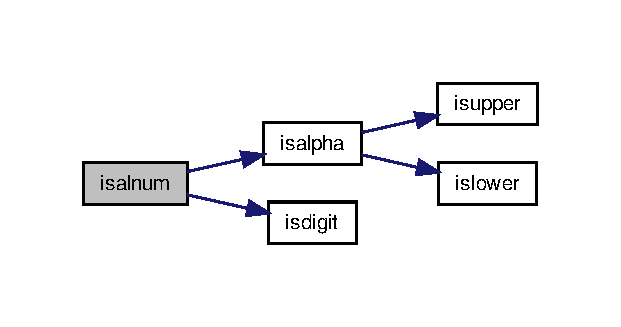
\includegraphics[width=298pt]{ctype_8c_adf38e126f73a010f30af76db2a28c6e1_cgraph}
\end{center}
\end{figure}




Voici le graphe des appelants de cette fonction \-:\nopagebreak
\begin{figure}[H]
\begin{center}
\leavevmode
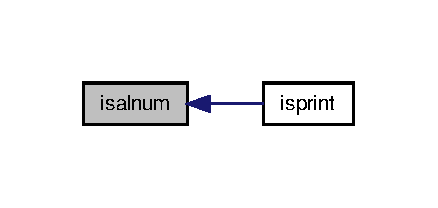
\includegraphics[width=208pt]{ctype_8c_adf38e126f73a010f30af76db2a28c6e1_icgraph}
\end{center}
\end{figure}


\hypertarget{ctype_8c_a25908ae63aac2df990634e1ae5bd14d9}{\index{ctype.\-c@{ctype.\-c}!isalpha@{isalpha}}
\index{isalpha@{isalpha}!ctype.c@{ctype.\-c}}
\subsubsection[{isalpha}]{\setlength{\rightskip}{0pt plus 5cm}int isalpha (
\begin{DoxyParamCaption}
\item[{int}]{c}
\end{DoxyParamCaption}
)}}\label{ctype_8c_a25908ae63aac2df990634e1ae5bd14d9}
Vérifie si l'on a un caractère alphabétique. Attention, ici on suppose qu'un caractère alphabétique est soit minuscule soit majuscule et exclu donc la gestion d'une locale où un caractère alphabétique ne serait ni minuscule ni majuscule.


\begin{DoxyParams}{Paramètres}
{\em c} & le caractère à vérifier.\\
\hline
\end{DoxyParams}
\begin{DoxyReturn}{Renvoie}
vrai si le caractère est alphabétique. 
\end{DoxyReturn}


Voici le graphe d'appel pour cette fonction \-:\nopagebreak
\begin{figure}[H]
\begin{center}
\leavevmode
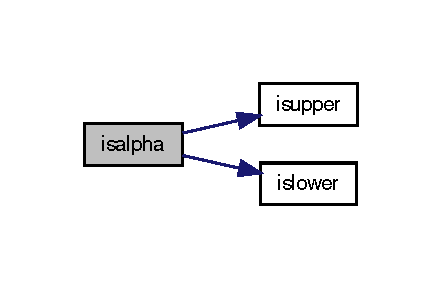
\includegraphics[width=212pt]{ctype_8c_a25908ae63aac2df990634e1ae5bd14d9_cgraph}
\end{center}
\end{figure}




Voici le graphe des appelants de cette fonction \-:\nopagebreak
\begin{figure}[H]
\begin{center}
\leavevmode
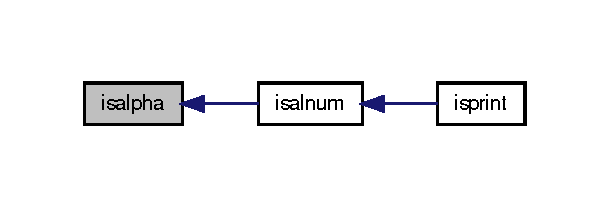
\includegraphics[width=292pt]{ctype_8c_a25908ae63aac2df990634e1ae5bd14d9_icgraph}
\end{center}
\end{figure}


\hypertarget{ctype_8c_aea4929b1b41f1a6d723e0312b1f050ed}{\index{ctype.\-c@{ctype.\-c}!isblank@{isblank}}
\index{isblank@{isblank}!ctype.c@{ctype.\-c}}
\subsubsection[{isblank}]{\setlength{\rightskip}{0pt plus 5cm}int isblank (
\begin{DoxyParamCaption}
\item[{int}]{c}
\end{DoxyParamCaption}
)}}\label{ctype_8c_aea4929b1b41f1a6d723e0312b1f050ed}
Vérifie si le caractère est blanc, c'est-\/à-\/dire un espace ou une tabulation.


\begin{DoxyParams}{Paramètres}
{\em c} & le caractère à vérifier.\\
\hline
\end{DoxyParams}
\begin{DoxyReturn}{Renvoie}
vrai si le caractère est blanc. 
\end{DoxyReturn}
\hypertarget{ctype_8c_a0008a4e8e7889734dc1d83297de07158}{\index{ctype.\-c@{ctype.\-c}!iscntrl@{iscntrl}}
\index{iscntrl@{iscntrl}!ctype.c@{ctype.\-c}}
\subsubsection[{iscntrl}]{\setlength{\rightskip}{0pt plus 5cm}int iscntrl (
\begin{DoxyParamCaption}
\item[{int}]{c}
\end{DoxyParamCaption}
)}}\label{ctype_8c_a0008a4e8e7889734dc1d83297de07158}
Vérifie si l'on a un caractère de contrôle.


\begin{DoxyParams}{Paramètres}
{\em c} & le caractère à vérifier.\\
\hline
\end{DoxyParams}
\begin{DoxyReturn}{Renvoie}
vrai si le caractère est de contrôle. 
\end{DoxyReturn}
\hypertarget{ctype_8c_a3fa45b35c8abf67a950b6d3d4063dede}{\index{ctype.\-c@{ctype.\-c}!isdigit@{isdigit}}
\index{isdigit@{isdigit}!ctype.c@{ctype.\-c}}
\subsubsection[{isdigit}]{\setlength{\rightskip}{0pt plus 5cm}int isdigit (
\begin{DoxyParamCaption}
\item[{int}]{c}
\end{DoxyParamCaption}
)}}\label{ctype_8c_a3fa45b35c8abf67a950b6d3d4063dede}

\begin{DoxyParams}{Paramètres}
{\em c} & le caractère à vérifier.\\
\hline
\end{DoxyParams}
\begin{DoxyReturn}{Renvoie}
vrai si le caractère est un chiffre. 
\end{DoxyReturn}


Voici le graphe des appelants de cette fonction \-:\nopagebreak
\begin{figure}[H]
\begin{center}
\leavevmode
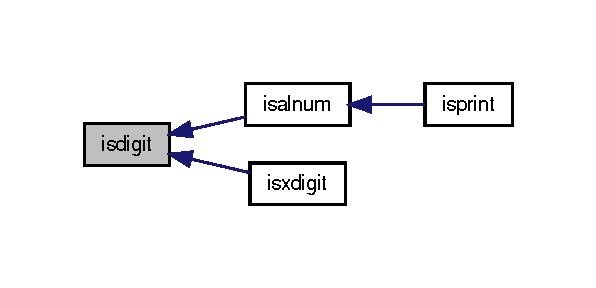
\includegraphics[width=286pt]{ctype_8c_a3fa45b35c8abf67a950b6d3d4063dede_icgraph}
\end{center}
\end{figure}


\hypertarget{ctype_8c_a7b8f652a0423a80922dd89d8829db5f2}{\index{ctype.\-c@{ctype.\-c}!islower@{islower}}
\index{islower@{islower}!ctype.c@{ctype.\-c}}
\subsubsection[{islower}]{\setlength{\rightskip}{0pt plus 5cm}int islower (
\begin{DoxyParamCaption}
\item[{int}]{c}
\end{DoxyParamCaption}
)}}\label{ctype_8c_a7b8f652a0423a80922dd89d8829db5f2}

\begin{DoxyParams}{Paramètres}
{\em c} & le caractère à vérifier.\\
\hline
\end{DoxyParams}
\begin{DoxyReturn}{Renvoie}
vrai si le caractère est minuscule. 
\end{DoxyReturn}


Voici le graphe des appelants de cette fonction \-:\nopagebreak
\begin{figure}[H]
\begin{center}
\leavevmode
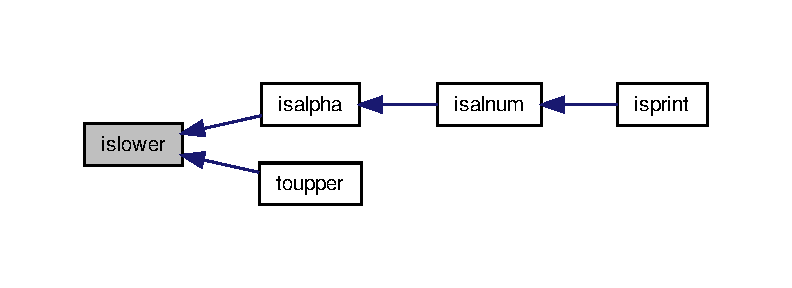
\includegraphics[width=350pt]{ctype_8c_a7b8f652a0423a80922dd89d8829db5f2_icgraph}
\end{center}
\end{figure}


\hypertarget{ctype_8c_a99355d8f0fb41ec43effb95189db0ed4}{\index{ctype.\-c@{ctype.\-c}!isprint@{isprint}}
\index{isprint@{isprint}!ctype.c@{ctype.\-c}}
\subsubsection[{isprint}]{\setlength{\rightskip}{0pt plus 5cm}int isprint (
\begin{DoxyParamCaption}
\item[{int}]{c}
\end{DoxyParamCaption}
)}}\label{ctype_8c_a99355d8f0fb41ec43effb95189db0ed4}

\begin{DoxyParams}{Paramètres}
{\em c} & le caractère à vérifier.\\
\hline
\end{DoxyParams}
\begin{DoxyReturn}{Renvoie}
vrai si le caractère est imprimable. 
\end{DoxyReturn}


Voici le graphe d'appel pour cette fonction \-:\nopagebreak
\begin{figure}[H]
\begin{center}
\leavevmode
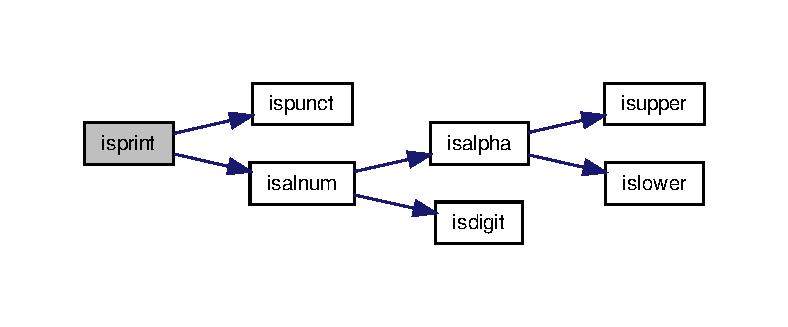
\includegraphics[width=350pt]{ctype_8c_a99355d8f0fb41ec43effb95189db0ed4_cgraph}
\end{center}
\end{figure}


\hypertarget{ctype_8c_af29554b3ec04ea7684482bffed5dbce6}{\index{ctype.\-c@{ctype.\-c}!ispunct@{ispunct}}
\index{ispunct@{ispunct}!ctype.c@{ctype.\-c}}
\subsubsection[{ispunct}]{\setlength{\rightskip}{0pt plus 5cm}int ispunct (
\begin{DoxyParamCaption}
\item[{int}]{c}
\end{DoxyParamCaption}
)}}\label{ctype_8c_af29554b3ec04ea7684482bffed5dbce6}
Vérifie s'il s'agit d'un caractère imprimable, qui ne soit ni un espace, ni un caractère alphanumérique.


\begin{DoxyParams}{Paramètres}
{\em c} & le caractère à vérifier.\\
\hline
\end{DoxyParams}
\begin{DoxyReturn}{Renvoie}
vrai si le caractère est une ponctuation. 
\end{DoxyReturn}


Voici le graphe des appelants de cette fonction \-:\nopagebreak
\begin{figure}[H]
\begin{center}
\leavevmode
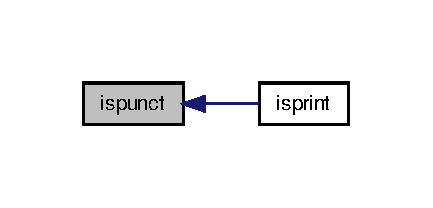
\includegraphics[width=206pt]{ctype_8c_af29554b3ec04ea7684482bffed5dbce6_icgraph}
\end{center}
\end{figure}


\hypertarget{ctype_8c_a56be4166e4673843042a548a7f513dbc}{\index{ctype.\-c@{ctype.\-c}!isspace@{isspace}}
\index{isspace@{isspace}!ctype.c@{ctype.\-c}}
\subsubsection[{isspace}]{\setlength{\rightskip}{0pt plus 5cm}int isspace (
\begin{DoxyParamCaption}
\item[{int}]{c}
\end{DoxyParamCaption}
)}}\label{ctype_8c_a56be4166e4673843042a548a7f513dbc}
Vérifie si l'on a un caractère blanc, d'espacement. Il s'agit de \-: espace, saut de page (form-\/feed, '\textbackslash{}f'), saut de ligne (newline, '\textbackslash{}n'), retour chariot (carriage return, '\textbackslash{}r'), tabulation horizontale ('\textbackslash{}t'), et tabulation verticale ('\textbackslash{}v').


\begin{DoxyParams}{Paramètres}
{\em c} & le caractère à vérifier.\\
\hline
\end{DoxyParams}
\begin{DoxyReturn}{Renvoie}
vrai si le caractère est d'espacement. 
\end{DoxyReturn}
\hypertarget{ctype_8c_adadd6582d46775aab6a51e29d16d9f77}{\index{ctype.\-c@{ctype.\-c}!isupper@{isupper}}
\index{isupper@{isupper}!ctype.c@{ctype.\-c}}
\subsubsection[{isupper}]{\setlength{\rightskip}{0pt plus 5cm}int isupper (
\begin{DoxyParamCaption}
\item[{int}]{c}
\end{DoxyParamCaption}
)}}\label{ctype_8c_adadd6582d46775aab6a51e29d16d9f77}
Vérifie si l'on a un caractère majuscule.


\begin{DoxyParams}{Paramètres}
{\em c} & le caractère à vérifier.\\
\hline
\end{DoxyParams}
\begin{DoxyReturn}{Renvoie}
vrai si le caractère est majuscule. 
\end{DoxyReturn}


Voici le graphe des appelants de cette fonction \-:\nopagebreak
\begin{figure}[H]
\begin{center}
\leavevmode
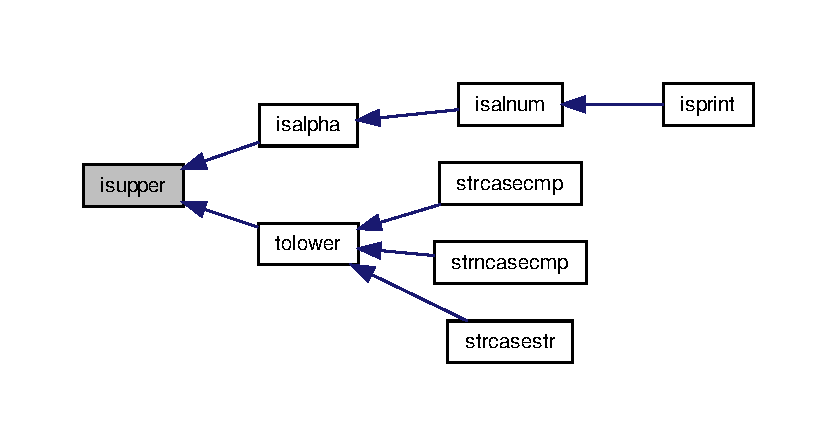
\includegraphics[width=350pt]{ctype_8c_adadd6582d46775aab6a51e29d16d9f77_icgraph}
\end{center}
\end{figure}


\hypertarget{ctype_8c_adaf3aadefe3fc4fb07b6be0d7b880f53}{\index{ctype.\-c@{ctype.\-c}!isxdigit@{isxdigit}}
\index{isxdigit@{isxdigit}!ctype.c@{ctype.\-c}}
\subsubsection[{isxdigit}]{\setlength{\rightskip}{0pt plus 5cm}int isxdigit (
\begin{DoxyParamCaption}
\item[{int}]{c}
\end{DoxyParamCaption}
)}}\label{ctype_8c_adaf3aadefe3fc4fb07b6be0d7b880f53}
Vérifie s'il s'agit d'un chiffre hexadécimal, c'est à dire 0 1 2 3 4 5 6 7 8 9 a b c d e f A B C D E F.


\begin{DoxyParams}{Paramètres}
{\em c} & le caractère à vérifier.\\
\hline
\end{DoxyParams}
\begin{DoxyReturn}{Renvoie}
vrai si le caractère est un chiffre hexadécimal. 
\end{DoxyReturn}


Voici le graphe d'appel pour cette fonction \-:\nopagebreak
\begin{figure}[H]
\begin{center}
\leavevmode
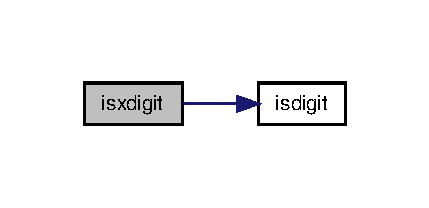
\includegraphics[width=204pt]{ctype_8c_adaf3aadefe3fc4fb07b6be0d7b880f53_cgraph}
\end{center}
\end{figure}



\hypertarget{dirent_8c}{\section{Référence du fichier libc/dirent.c}
\label{dirent_8c}\index{libc/dirent.\-c@{libc/dirent.\-c}}
}


Fonctions pour faciliter la gestion des dossiers.  


{\ttfamily \#include $<$dirent.\-h$>$}\\*
{\ttfamily \#include $<$fcntl.\-h$>$}\\*
{\ttfamily \#include $<$stdlib.\-h$>$}\\*
{\ttfamily \#include $<$string.\-h$>$}\\*
{\ttfamily \#include $<$sys/syscall.\-h$>$}\\*
{\ttfamily \#include $<$unistd.\-h$>$}\\*
{\ttfamily \#include $<$stdio.\-h$>$}\\*
Graphe des dépendances par inclusion de dirent.\-c\-:
\nopagebreak
\begin{figure}[H]
\begin{center}
\leavevmode
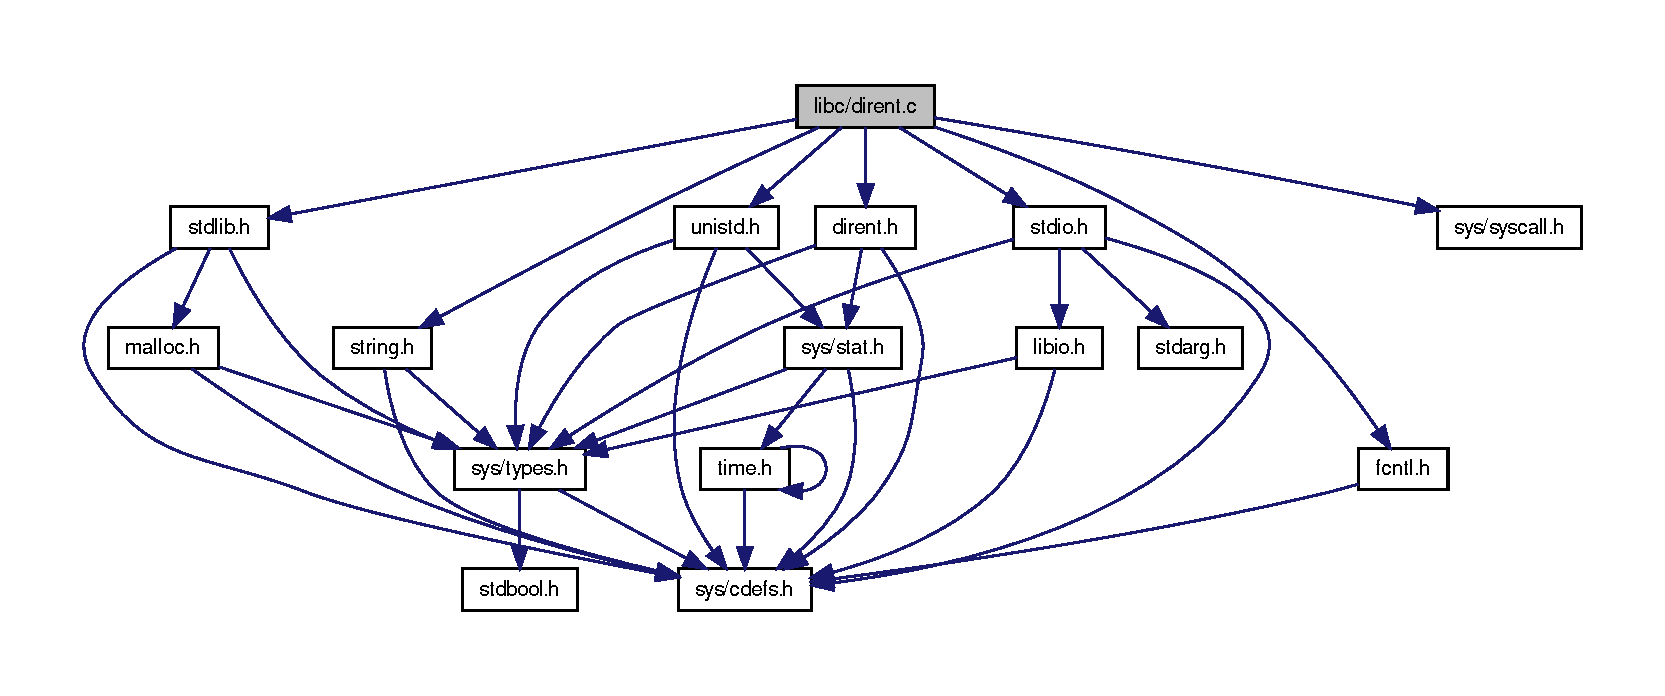
\includegraphics[width=350pt]{dirent_8c__incl}
\end{center}
\end{figure}
\subsection*{Fonctions}
\begin{DoxyCompactItemize}
\item 
int \hyperlink{dirent_8c_aee98bbe743c2d14dbaa67f01c3fb9ed5}{mkdir} (const char $\ast$pathname, \hyperlink{kstat_8h_af8f4385bb42836d1e3ad4fea9d71d1b9}{mode\-\_\-t} \hyperlink{structmode}{mode})
\item 
\hyperlink{dirent_8h_a9e986c0f8d94ffe9983a6eabb17cbb9a}{D\-I\-R} $\ast$ \hyperlink{dirent_8c_ad09dd96447776d2bc5d8321e4b499591}{opendir} (const char $\ast$dirname)
\item 
struct \hyperlink{structdirent}{dirent} $\ast$ \hyperlink{dirent_8c_a58257faf8b13b3f14558613c632b2373}{readdir} (\hyperlink{dirent_8h_a9e986c0f8d94ffe9983a6eabb17cbb9a}{D\-I\-R} $\ast$dirp)
\item 
int \hyperlink{dirent_8c_aaeac2b41e8c2c3a5f91c9bd511a8c0a6}{closedir} (\hyperlink{dirent_8h_a9e986c0f8d94ffe9983a6eabb17cbb9a}{D\-I\-R} $\ast$dirp)
\end{DoxyCompactItemize}


\subsection{Description détaillée}
\begin{DoxyAuthor}{Auteur}
Tac\-O\-S developers
\end{DoxyAuthor}
\hypertarget{wait_8c_LICENSE}{}\subsection{L\-I\-C\-E\-N\-S\-E}\label{wait_8c_LICENSE}
Copyright (C) 2010, 2011, 2012, 2013 -\/ Tac\-O\-S developers.

This program is free software; you can redistribute it and/or modify it under the terms of the G\-N\-U General Public License as published by the Free Software Foundation; either version 3 of the License, or (at your option) any later version.

This program is distributed in the hope that it will be useful, but W\-I\-T\-H\-O\-U\-T A\-N\-Y W\-A\-R\-R\-A\-N\-T\-Y; without even the implied warranty of M\-E\-R\-C\-H\-A\-N\-T\-A\-B\-I\-L\-I\-T\-Y or F\-I\-T\-N\-E\-S\-S F\-O\-R A P\-A\-R\-T\-I\-C\-U\-L\-A\-R P\-U\-R\-P\-O\-S\-E. See the G\-N\-U General Public License for more details at \href{http://www.gnu.org/copyleft/gpl.html}{\tt http\-://www.\-gnu.\-org/copyleft/gpl.\-html}

You should have received a copy of the G\-N\-U General Public License along with this program; if not, see \href{http://www.gnu.org/licenses}{\tt http\-://www.\-gnu.\-org/licenses}.\hypertarget{wait_8c_DESCRIPTION}{}\subsection{D\-E\-S\-C\-R\-I\-P\-T\-I\-O\-N}\label{wait_8c_DESCRIPTION}


\subsection{Documentation des fonctions}
\hypertarget{dirent_8c_aaeac2b41e8c2c3a5f91c9bd511a8c0a6}{\index{dirent.\-c@{dirent.\-c}!closedir@{closedir}}
\index{closedir@{closedir}!dirent.c@{dirent.\-c}}
\subsubsection[{closedir}]{\setlength{\rightskip}{0pt plus 5cm}int closedir (
\begin{DoxyParamCaption}
\item[{{\bf D\-I\-R} $\ast$}]{dirp}
\end{DoxyParamCaption}
)}}\label{dirent_8c_aaeac2b41e8c2c3a5f91c9bd511a8c0a6}
Fermeture d'un dossier ouvert.


\begin{DoxyParams}{Paramètres}
{\em dirp} & La structure D\-I\-R initialisée par opendir.\\
\hline
\end{DoxyParams}
\begin{DoxyReturn}{Renvoie}
0 en cas de succès. 
\end{DoxyReturn}


Voici le graphe d'appel pour cette fonction \-:
\nopagebreak
\begin{figure}[H]
\begin{center}
\leavevmode
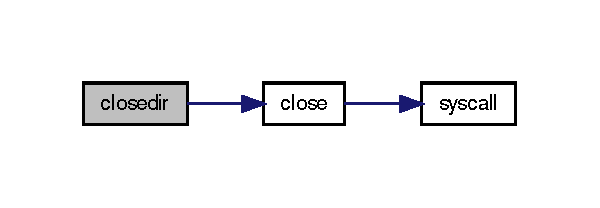
\includegraphics[width=290pt]{dirent_8c_aaeac2b41e8c2c3a5f91c9bd511a8c0a6_cgraph}
\end{center}
\end{figure}


\hypertarget{dirent_8c_aee98bbe743c2d14dbaa67f01c3fb9ed5}{\index{dirent.\-c@{dirent.\-c}!mkdir@{mkdir}}
\index{mkdir@{mkdir}!dirent.c@{dirent.\-c}}
\subsubsection[{mkdir}]{\setlength{\rightskip}{0pt plus 5cm}int mkdir (
\begin{DoxyParamCaption}
\item[{const char $\ast$}]{pathname, }
\item[{{\bf mode\-\_\-t}}]{mode}
\end{DoxyParamCaption}
)}}\label{dirent_8c_aee98bbe743c2d14dbaa67f01c3fb9ed5}
Crée un nouveau répertoire.


\begin{DoxyParams}{Paramètres}
{\em pathname} & Le chemin du dossier à créer. \\
\hline
{\em mode} & Les droits d'accès.\\
\hline
\end{DoxyParams}
\begin{DoxyReturn}{Renvoie}
0 en cas de succès. 
\end{DoxyReturn}


Voici le graphe d'appel pour cette fonction \-:
\nopagebreak
\begin{figure}[H]
\begin{center}
\leavevmode
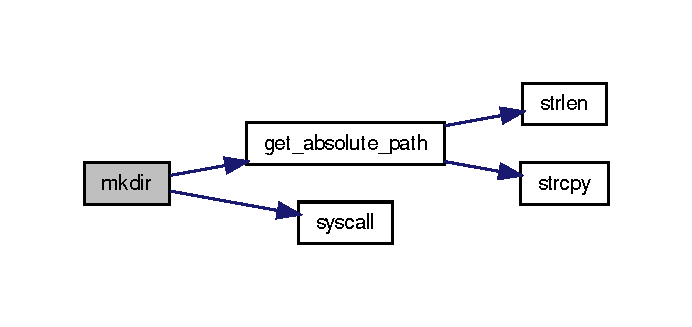
\includegraphics[width=334pt]{dirent_8c_aee98bbe743c2d14dbaa67f01c3fb9ed5_cgraph}
\end{center}
\end{figure}


\hypertarget{dirent_8c_ad09dd96447776d2bc5d8321e4b499591}{\index{dirent.\-c@{dirent.\-c}!opendir@{opendir}}
\index{opendir@{opendir}!dirent.c@{dirent.\-c}}
\subsubsection[{opendir}]{\setlength{\rightskip}{0pt plus 5cm}{\bf D\-I\-R}$\ast$ opendir (
\begin{DoxyParamCaption}
\item[{const char $\ast$}]{dirname}
\end{DoxyParamCaption}
)}}\label{dirent_8c_ad09dd96447776d2bc5d8321e4b499591}
Ouvre un dossier pour lister les fichiers à l'intérieur.


\begin{DoxyParams}{Paramètres}
{\em dirname} & Le chemin du dossier à ouvrir.\\
\hline
\end{DoxyParams}
\begin{DoxyReturn}{Renvoie}
Une structure D\-I\-R permettant de lire le contenu du dossier. 
\end{DoxyReturn}


Voici le graphe d'appel pour cette fonction \-:
\nopagebreak
\begin{figure}[H]
\begin{center}
\leavevmode
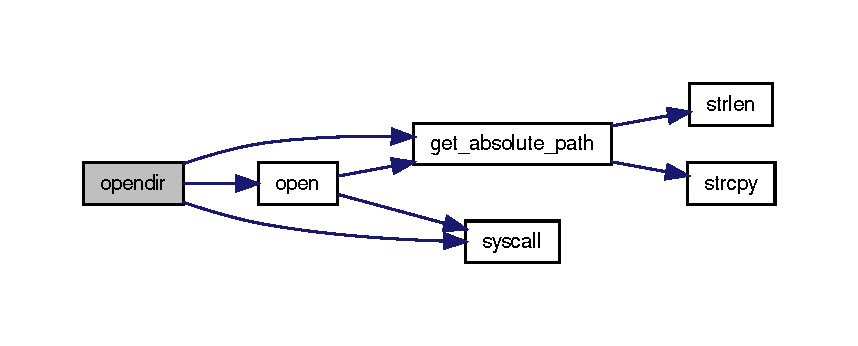
\includegraphics[width=350pt]{dirent_8c_ad09dd96447776d2bc5d8321e4b499591_cgraph}
\end{center}
\end{figure}




Voici le graphe des appelants de cette fonction \-:
\nopagebreak
\begin{figure}[H]
\begin{center}
\leavevmode
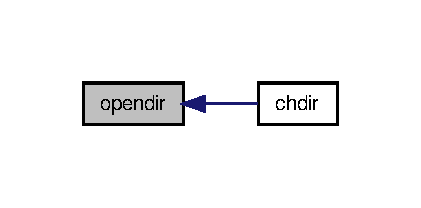
\includegraphics[width=202pt]{dirent_8c_ad09dd96447776d2bc5d8321e4b499591_icgraph}
\end{center}
\end{figure}


\hypertarget{dirent_8c_a58257faf8b13b3f14558613c632b2373}{\index{dirent.\-c@{dirent.\-c}!readdir@{readdir}}
\index{readdir@{readdir}!dirent.c@{dirent.\-c}}
\subsubsection[{readdir}]{\setlength{\rightskip}{0pt plus 5cm}struct {\bf dirent}$\ast$ readdir (
\begin{DoxyParamCaption}
\item[{{\bf D\-I\-R} $\ast$}]{dirp}
\end{DoxyParamCaption}
)\hspace{0.3cm}{\ttfamily [read]}}}\label{dirent_8c_a58257faf8b13b3f14558613c632b2373}
Lecture de la prochaine entrée du dossier.


\begin{DoxyParams}{Paramètres}
{\em dirp} & La structure D\-I\-R initialisée par opendir.\\
\hline
\end{DoxyParams}
\begin{DoxyReturn}{Renvoie}
Un directory entry. 
\end{DoxyReturn}


Voici le graphe d'appel pour cette fonction \-:
\nopagebreak
\begin{figure}[H]
\begin{center}
\leavevmode
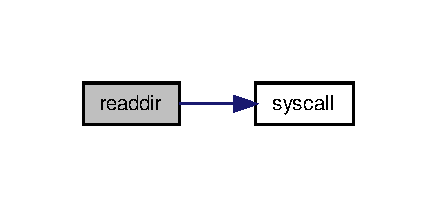
\includegraphics[width=210pt]{dirent_8c_a58257faf8b13b3f14558613c632b2373_cgraph}
\end{center}
\end{figure}



\hypertarget{errno_8c}{\section{Référence du fichier libc/errno.c}
\label{errno_8c}\index{libc/errno.\+c@{libc/errno.\+c}}
}


Contient la variable d'erreur errno.  


\subsection*{Variables}
\begin{DoxyCompactItemize}
\item 
int \hyperlink{errno_8c_ad65a8842cc674e3ddf69355898c0ecbf}{errno}
\item 
const char $\ast$ \hyperlink{errno_8c_a76ebfe24a40210e5935998c1fa86d3a0}{sys\+\_\+errlist} \mbox{[}$\,$\mbox{]}
\end{DoxyCompactItemize}


\subsection{Description détaillée}
\begin{DoxyAuthor}{Auteur}
Tac\+O\+S developers
\end{DoxyAuthor}
\hypertarget{wait_8c_LICENSE}{}\subsection{L\+I\+C\+E\+N\+S\+E}\label{wait_8c_LICENSE}
Copyright (C) 2010-\/2014 Tac\+O\+S developers.

This program is free software; you can redistribute it and/or modify it under the terms of the G\+N\+U General Public License as published by the Free Software Foundation; either version 3 of the License, or (at your option) any later version.

This program is distributed in the hope that it will be useful, but W\+I\+T\+H\+O\+U\+T A\+N\+Y W\+A\+R\+R\+A\+N\+T\+Y; without even the implied warranty of M\+E\+R\+C\+H\+A\+N\+T\+A\+B\+I\+L\+I\+T\+Y or F\+I\+T\+N\+E\+S\+S F\+O\+R A P\+A\+R\+T\+I\+C\+U\+L\+A\+R P\+U\+R\+P\+O\+S\+E. See the G\+N\+U General Public License for more details at \href{http://www.gnu.org/copyleft/gpl.html}{\tt http\+://www.\+gnu.\+org/copyleft/gpl.\+html}

You should have received a copy of the G\+N\+U General Public License along with this program; if not, see \href{http://www.gnu.org/licenses}{\tt http\+://www.\+gnu.\+org/licenses}.\hypertarget{wait_8c_DESCRIPTION}{}\subsection{D\+E\+S\+C\+R\+I\+P\+T\+I\+O\+N}\label{wait_8c_DESCRIPTION}


\subsection{Documentation des variables}
\hypertarget{errno_8c_ad65a8842cc674e3ddf69355898c0ecbf}{\index{errno.\+c@{errno.\+c}!errno@{errno}}
\index{errno@{errno}!errno.\+c@{errno.\+c}}
\subsubsection[{errno}]{\setlength{\rightskip}{0pt plus 5cm}int errno}}\label{errno_8c_ad65a8842cc674e3ddf69355898c0ecbf}
Variable qui contient le numéro de la dernière erreur. \hypertarget{errno_8c_a76ebfe24a40210e5935998c1fa86d3a0}{\index{errno.\+c@{errno.\+c}!sys\+\_\+errlist@{sys\+\_\+errlist}}
\index{sys\+\_\+errlist@{sys\+\_\+errlist}!errno.\+c@{errno.\+c}}
\subsubsection[{sys\+\_\+errlist}]{\setlength{\rightskip}{0pt plus 5cm}const char$\ast$ sys\+\_\+errlist\mbox{[}$\,$\mbox{]}}}\label{errno_8c_a76ebfe24a40210e5935998c1fa86d3a0}
{\bfseries Valeur initiale \+:}
\begin{DoxyCode}
= \{
\textcolor{stringliteral}{"Erreur inconnue ou pas d'erreur."},
\textcolor{stringliteral}{"Essai encore ;)."},
\textcolor{stringliteral}{"Mauvais numéro de fichier."},
\textcolor{stringliteral}{"Mauvaise adresse."},
\textcolor{stringliteral}{"Fichier trop gros."},
\textcolor{stringliteral}{"System call interrompu."},
\textcolor{stringliteral}{"Argument invalide."},
\textcolor{stringliteral}{"Erreur d'entrée / sortie."},
\textcolor{stringliteral}{"Plus d'espace libre sur le périphérique."},
\textcolor{stringliteral}{"Tube brisé."},
\textcolor{stringliteral}{"Résultat mathématique non representable."},
\textcolor{stringliteral}{"Entrée non trouvée."},
\textcolor{stringliteral}{"Ce n'est pas un dossier."},
\textcolor{stringliteral}{"Le fichier existe déjà."},
\textcolor{stringliteral}{"Opération non permise."},
\textcolor{stringliteral}{"C'est un dossier."},
\textcolor{stringliteral}{"Overflow de la file table."},
\textcolor{stringliteral}{"Trop de fichiers ouverts."}\}
\end{DoxyCode}
Liste des messages d'erreur. 
\hypertarget{fcntl_8c}{\section{Référence du fichier libc/fcntl.c}
\label{fcntl_8c}\index{libc/fcntl.\+c@{libc/fcntl.\+c}}
}


File control operations.  


{\ttfamily \#include $<$stdlib.\+h$>$}\\*
{\ttfamily \#include $<$fcntl.\+h$>$}\\*
{\ttfamily \#include $<$unistd.\+h$>$}\\*
{\ttfamily \#include $<$sys/syscall.\+h$>$}\\*
Graphe des dépendances par inclusion de fcntl.\+c\+:
\nopagebreak
\begin{figure}[H]
\begin{center}
\leavevmode
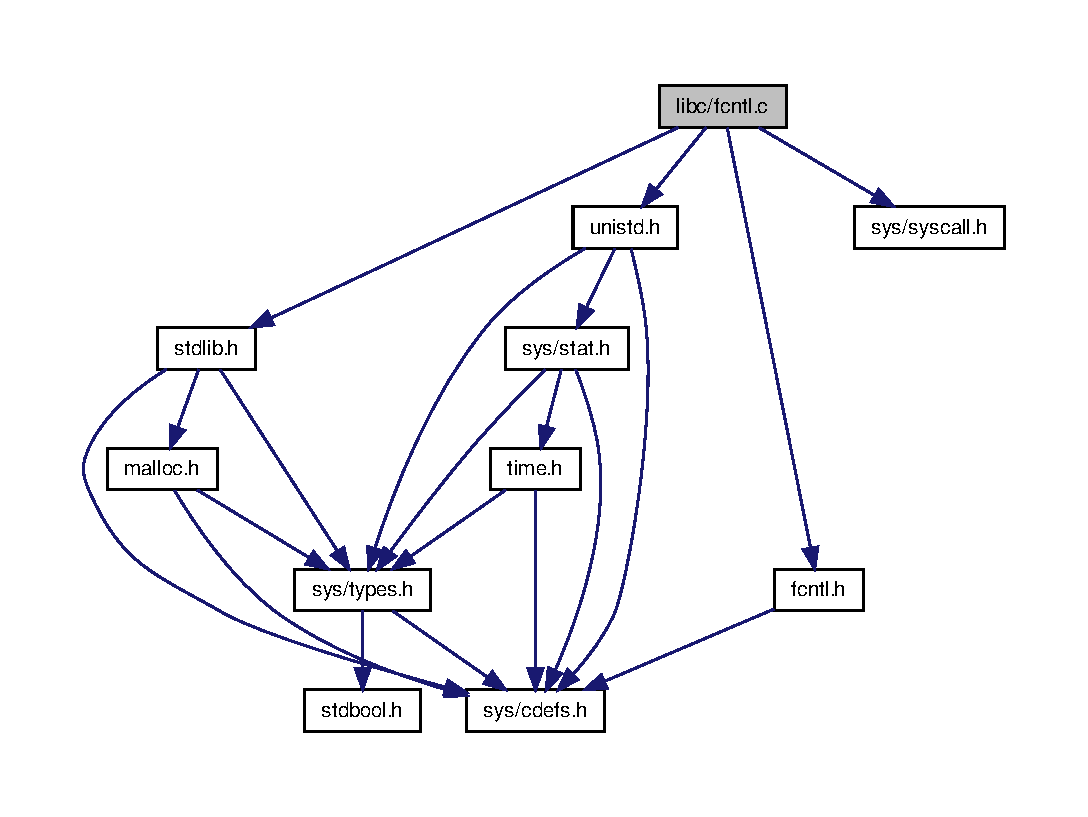
\includegraphics[width=350pt]{fcntl_8c__incl}
\end{center}
\end{figure}
\subsection*{Fonctions}
\begin{DoxyCompactItemize}
\item 
int \hyperlink{fcntl_8c_adcb60598073f6f9cbb0091ef6768fa5c}{open} (const char $\ast$pathname, int flags)
\item 
int \hyperlink{fcntl_8c_ae68e7e3d0b126184d5d00e78e94305fb}{close} (int id)
\item 
int \hyperlink{fcntl_8c_a5752d6571b615f1b7b1b0f719c2bc69d}{fcntl} (int fd, unsigned int request, void $\ast$data)
\end{DoxyCompactItemize}


\subsection{Description détaillée}
\begin{DoxyAuthor}{Auteur}
Tac\+O\+S developers
\end{DoxyAuthor}
\hypertarget{wait_8c_LICENSE}{}\subsection{L\+I\+C\+E\+N\+S\+E}\label{wait_8c_LICENSE}
Copyright (C) 2010-\/2014 Tac\+O\+S developers.

This program is free software; you can redistribute it and/or modify it under the terms of the G\+N\+U General Public License as published by the Free Software Foundation; either version 3 of the License, or (at your option) any later version.

This program is distributed in the hope that it will be useful, but W\+I\+T\+H\+O\+U\+T A\+N\+Y W\+A\+R\+R\+A\+N\+T\+Y; without even the implied warranty of M\+E\+R\+C\+H\+A\+N\+T\+A\+B\+I\+L\+I\+T\+Y or F\+I\+T\+N\+E\+S\+S F\+O\+R A P\+A\+R\+T\+I\+C\+U\+L\+A\+R P\+U\+R\+P\+O\+S\+E. See the G\+N\+U General Public License for more details at \href{http://www.gnu.org/copyleft/gpl.html}{\tt http\+://www.\+gnu.\+org/copyleft/gpl.\+html}

You should have received a copy of the G\+N\+U General Public License along with this program; if not, see \href{http://www.gnu.org/licenses}{\tt http\+://www.\+gnu.\+org/licenses}.\hypertarget{wait_8c_DESCRIPTION}{}\subsection{D\+E\+S\+C\+R\+I\+P\+T\+I\+O\+N}\label{wait_8c_DESCRIPTION}


\subsection{Documentation des fonctions}
\hypertarget{fcntl_8c_ae68e7e3d0b126184d5d00e78e94305fb}{\index{fcntl.\+c@{fcntl.\+c}!close@{close}}
\index{close@{close}!fcntl.\+c@{fcntl.\+c}}
\subsubsection[{close}]{\setlength{\rightskip}{0pt plus 5cm}int close (
\begin{DoxyParamCaption}
\item[{int}]{id}
\end{DoxyParamCaption}
)}}\label{fcntl_8c_ae68e7e3d0b126184d5d00e78e94305fb}
Ferme un fichier ouvert.


\begin{DoxyParams}{Paramètres}
{\em id} & descripteur du fichier.\\
\hline
\end{DoxyParams}
\begin{DoxyReturn}{Renvoie}
0 en cas de succès. 
\end{DoxyReturn}


Voici le graphe d'appel pour cette fonction \+:
\nopagebreak
\begin{figure}[H]
\begin{center}
\leavevmode
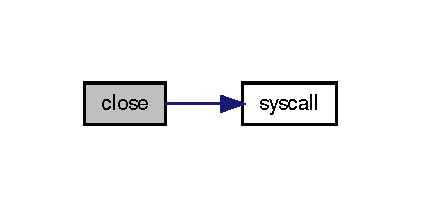
\includegraphics[width=203pt]{fcntl_8c_ae68e7e3d0b126184d5d00e78e94305fb_cgraph}
\end{center}
\end{figure}




Voici le graphe des appelants de cette fonction \+:
\nopagebreak
\begin{figure}[H]
\begin{center}
\leavevmode
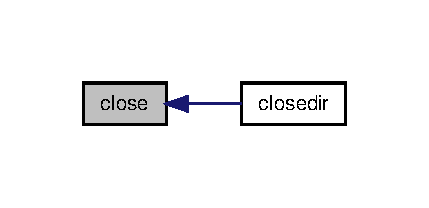
\includegraphics[width=206pt]{fcntl_8c_ae68e7e3d0b126184d5d00e78e94305fb_icgraph}
\end{center}
\end{figure}


\hypertarget{fcntl_8c_a5752d6571b615f1b7b1b0f719c2bc69d}{\index{fcntl.\+c@{fcntl.\+c}!fcntl@{fcntl}}
\index{fcntl@{fcntl}!fcntl.\+c@{fcntl.\+c}}
\subsubsection[{fcntl}]{\setlength{\rightskip}{0pt plus 5cm}int fcntl (
\begin{DoxyParamCaption}
\item[{int}]{fd, }
\item[{unsigned int}]{request, }
\item[{void $\ast$}]{data}
\end{DoxyParamCaption}
)}}\label{fcntl_8c_a5752d6571b615f1b7b1b0f719c2bc69d}
Manipulation d'un descripteur de fichier.


\begin{DoxyParams}{Paramètres}
{\em fd} & descripteur du fichier. \\
\hline
{\em request} & action à faire. \\
\hline
{\em data} & les arguments nécessaires à l'action.\\
\hline
\end{DoxyParams}
\begin{DoxyReturn}{Renvoie}
valeur en fonction de l'action. 
\end{DoxyReturn}


Voici le graphe d'appel pour cette fonction \+:
\nopagebreak
\begin{figure}[H]
\begin{center}
\leavevmode
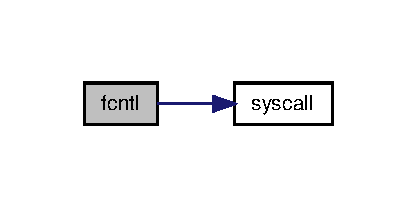
\includegraphics[width=198pt]{fcntl_8c_a5752d6571b615f1b7b1b0f719c2bc69d_cgraph}
\end{center}
\end{figure}


\hypertarget{fcntl_8c_adcb60598073f6f9cbb0091ef6768fa5c}{\index{fcntl.\+c@{fcntl.\+c}!open@{open}}
\index{open@{open}!fcntl.\+c@{fcntl.\+c}}
\subsubsection[{open}]{\setlength{\rightskip}{0pt plus 5cm}int open (
\begin{DoxyParamCaption}
\item[{const char $\ast$}]{pathname, }
\item[{int}]{flags}
\end{DoxyParamCaption}
)}}\label{fcntl_8c_adcb60598073f6f9cbb0091ef6768fa5c}
Ouvrir un fichier ou un périphérique.


\begin{DoxyParams}{Paramètres}
{\em pathname} & Chemin du fichier. \\
\hline
{\em flags} & Flags pour indiquer le mode d'ouverture.\\
\hline
\end{DoxyParams}
\begin{DoxyReturn}{Renvoie}
l'id du file descriptor. -\/1 en cas d'erreur. 
\end{DoxyReturn}


Voici le graphe d'appel pour cette fonction \+:
\nopagebreak
\begin{figure}[H]
\begin{center}
\leavevmode
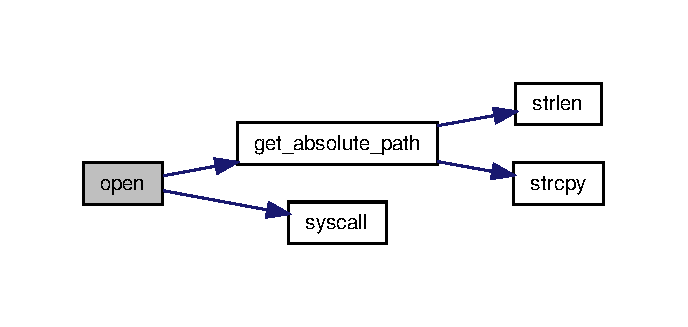
\includegraphics[width=329pt]{fcntl_8c_adcb60598073f6f9cbb0091ef6768fa5c_cgraph}
\end{center}
\end{figure}




Voici le graphe des appelants de cette fonction \+:
\nopagebreak
\begin{figure}[H]
\begin{center}
\leavevmode
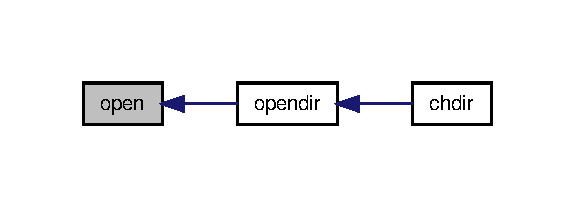
\includegraphics[width=276pt]{fcntl_8c_adcb60598073f6f9cbb0091ef6768fa5c_icgraph}
\end{center}
\end{figure}



\hypertarget{ctype_8h}{\section{Référence du fichier libc/include/ctype.h}
\label{ctype_8h}\index{libc/include/ctype.\-h@{libc/include/ctype.\-h}}
}


Fonctions de classification de caractères.  


{\ttfamily \#include $<$sys/cdefs.\-h$>$}\\*
Graphe des dépendances par inclusion de ctype.\-h\-:\nopagebreak
\begin{figure}[H]
\begin{center}
\leavevmode
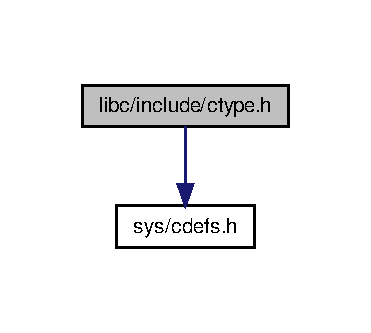
\includegraphics[width=178pt]{ctype_8h__incl}
\end{center}
\end{figure}
Ce graphe montre quels fichiers incluent directement ou indirectement ce fichier \-:\nopagebreak
\begin{figure}[H]
\begin{center}
\leavevmode
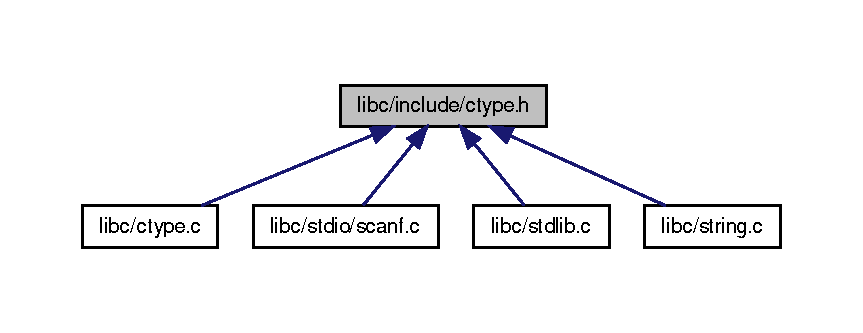
\includegraphics[width=350pt]{ctype_8h__dep__incl}
\end{center}
\end{figure}
\subsection*{Fonctions}
\begin{DoxyCompactItemize}
\item 
\-\_\-\-\_\-\-B\-E\-G\-I\-N\-\_\-\-D\-E\-C\-L\-S int \hyperlink{ctype_8h_a9ce2e598cec9a4644e4d475011f29a73}{isalnum} (int c)
\begin{DoxyCompactList}\small\item\em vérifie si l'on a un caractère alphanumérique. \end{DoxyCompactList}\item 
int \hyperlink{ctype_8h_a25908ae63aac2df990634e1ae5bd14d9}{isalpha} (int c)
\begin{DoxyCompactList}\small\item\em vérifie si l'on a un caractère alphabétique. \end{DoxyCompactList}\item 
int \hyperlink{ctype_8h_aea4929b1b41f1a6d723e0312b1f050ed}{isblank} (int c)
\begin{DoxyCompactList}\small\item\em vérifie si le caractère est blanc, c'est-\/à-\/dire un espace ou une tabulation. \end{DoxyCompactList}\item 
int \hyperlink{ctype_8h_a0008a4e8e7889734dc1d83297de07158}{iscntrl} (int c)
\begin{DoxyCompactList}\small\item\em vérifie si l'on a un caractère de contrôle. \end{DoxyCompactList}\item 
int \hyperlink{ctype_8h_a3fa45b35c8abf67a950b6d3d4063dede}{isdigit} (int c)
\begin{DoxyCompactList}\small\item\em vérifie si l'on a un chiffre (0 à 9). \end{DoxyCompactList}\item 
int \hyperlink{ctype_8h_a7b8f652a0423a80922dd89d8829db5f2}{islower} (int c)
\begin{DoxyCompactList}\small\item\em vérifie si l'on a un caractère minuscule. \end{DoxyCompactList}\item 
int \hyperlink{ctype_8h_a99355d8f0fb41ec43effb95189db0ed4}{isprint} (int c)
\begin{DoxyCompactList}\small\item\em vérifie s'il s'agit d'un caractère imprimable, y compris l'espace. \end{DoxyCompactList}\item 
int \hyperlink{ctype_8h_af29554b3ec04ea7684482bffed5dbce6}{ispunct} (int c)
\begin{DoxyCompactList}\small\item\em vérifie s'il s'agit d'un caractère imprimable, qui ne soit ni un espace, ni un caractère alphanumérique. \end{DoxyCompactList}\item 
int \hyperlink{ctype_8h_a56be4166e4673843042a548a7f513dbc}{isspace} (int c)
\begin{DoxyCompactList}\small\item\em vérifie si l'on a un caractère blanc, d'espacement. \end{DoxyCompactList}\item 
int \hyperlink{ctype_8h_adadd6582d46775aab6a51e29d16d9f77}{isupper} (int c)
\begin{DoxyCompactList}\small\item\em vérifie si l'on a un caractère majuscule. \end{DoxyCompactList}\item 
int \hyperlink{ctype_8h_adaf3aadefe3fc4fb07b6be0d7b880f53}{isxdigit} (int c)
\begin{DoxyCompactList}\small\item\em vérifie s'il s'agit d'un chiffre hexadécimal. \end{DoxyCompactList}\item 
int \hyperlink{ctype_8h_ac79d6114c9df7350cedcd8cf921a6ea4}{tolower} (int c)
\begin{DoxyCompactList}\small\item\em Convertit la lettre c en minuscule. \end{DoxyCompactList}\item 
int \hyperlink{ctype_8h_a9c2f57ac3865af9006fdbfd5db9fd517}{toupper} (int c)
\begin{DoxyCompactList}\small\item\em Convertit la lettre c en majuscule. \end{DoxyCompactList}\end{DoxyCompactItemize}


\subsection{Description détaillée}
\begin{DoxyAuthor}{Auteur}
Tac\-O\-S developers
\end{DoxyAuthor}
\hypertarget{wait_8c_LICENSE}{}\subsection{L\-I\-C\-E\-N\-S\-E}\label{wait_8c_LICENSE}
Copyright (C) 2010, 2011, 2012 -\/ Tac\-O\-S developers.

This program is free software; you can redistribute it and/or modify it under the terms of the G\-N\-U General Public License as published by the Free Software Foundation; either version 3 of the License, or (at your option) any later version.

This program is distributed in the hope that it will be useful, but W\-I\-T\-H\-O\-U\-T A\-N\-Y W\-A\-R\-R\-A\-N\-T\-Y; without even the implied warranty of M\-E\-R\-C\-H\-A\-N\-T\-A\-B\-I\-L\-I\-T\-Y or F\-I\-T\-N\-E\-S\-S F\-O\-R A P\-A\-R\-T\-I\-C\-U\-L\-A\-R P\-U\-R\-P\-O\-S\-E. See the G\-N\-U General Public License for more details at \href{http://www.gnu.org/copyleft/gpl.html}{\tt http\-://www.\-gnu.\-org/copyleft/gpl.\-html}

You should have received a copy of the G\-N\-U General Public License along with this program; if not, see \href{http://www.gnu.org/licenses}{\tt http\-://www.\-gnu.\-org/licenses}.\hypertarget{wait_8c_DESCRIPTION}{}\subsection{D\-E\-S\-C\-R\-I\-P\-T\-I\-O\-N}\label{wait_8c_DESCRIPTION}


\subsection{Documentation des fonctions}
\hypertarget{ctype_8h_a9ce2e598cec9a4644e4d475011f29a73}{\index{ctype.\-h@{ctype.\-h}!isalnum@{isalnum}}
\index{isalnum@{isalnum}!ctype.h@{ctype.\-h}}
\subsubsection[{isalnum}]{\setlength{\rightskip}{0pt plus 5cm}\-\_\-\-\_\-\-B\-E\-G\-I\-N\-\_\-\-D\-E\-C\-L\-S int isalnum (
\begin{DoxyParamCaption}
\item[{int}]{c}
\end{DoxyParamCaption}
)}}\label{ctype_8h_a9ce2e598cec9a4644e4d475011f29a73}
Vérifie si l'on a un caractère alphanumérique. C'est équivalent à (isalpha(c) $|$$|$ isdigit(c)).


\begin{DoxyParams}{Paramètres}
{\em c} & le caractère à vérifier.\\
\hline
\end{DoxyParams}
\begin{DoxyReturn}{Renvoie}
vrai si le caractère est alphanumérique. 
\end{DoxyReturn}


Voici le graphe d'appel pour cette fonction \-:\nopagebreak
\begin{figure}[H]
\begin{center}
\leavevmode
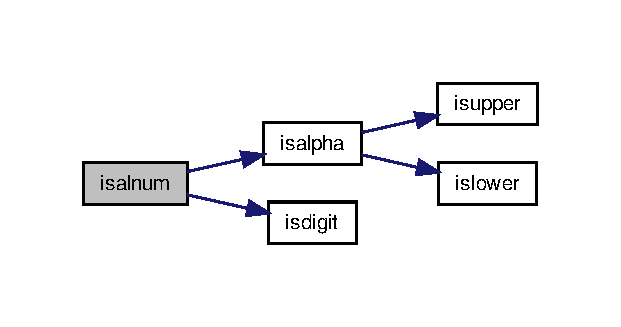
\includegraphics[width=298pt]{ctype_8h_a9ce2e598cec9a4644e4d475011f29a73_cgraph}
\end{center}
\end{figure}




Voici le graphe des appelants de cette fonction \-:\nopagebreak
\begin{figure}[H]
\begin{center}
\leavevmode
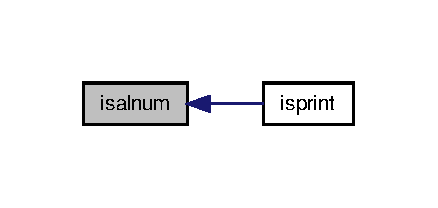
\includegraphics[width=210pt]{ctype_8h_a9ce2e598cec9a4644e4d475011f29a73_icgraph}
\end{center}
\end{figure}


\hypertarget{ctype_8h_a25908ae63aac2df990634e1ae5bd14d9}{\index{ctype.\-h@{ctype.\-h}!isalpha@{isalpha}}
\index{isalpha@{isalpha}!ctype.h@{ctype.\-h}}
\subsubsection[{isalpha}]{\setlength{\rightskip}{0pt plus 5cm}int isalpha (
\begin{DoxyParamCaption}
\item[{int}]{c}
\end{DoxyParamCaption}
)}}\label{ctype_8h_a25908ae63aac2df990634e1ae5bd14d9}
Vérifie si l'on a un caractère alphabétique. Attention, ici on suppose qu'un caractère alphabétique est soit minuscule soit majuscule et exclu donc la gestion d'une locale où un caractère alphabétique ne serait ni minuscule ni majuscule.


\begin{DoxyParams}{Paramètres}
{\em c} & le caractère à vérifier.\\
\hline
\end{DoxyParams}
\begin{DoxyReturn}{Renvoie}
vrai si le caractère est alphabétique. 
\end{DoxyReturn}


Voici le graphe d'appel pour cette fonction \-:\nopagebreak
\begin{figure}[H]
\begin{center}
\leavevmode
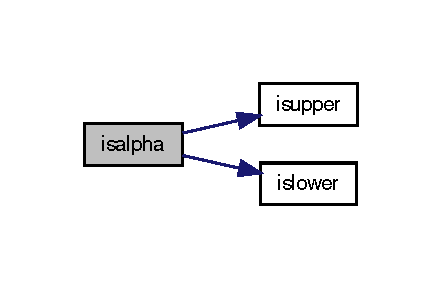
\includegraphics[width=212pt]{ctype_8h_a25908ae63aac2df990634e1ae5bd14d9_cgraph}
\end{center}
\end{figure}




Voici le graphe des appelants de cette fonction \-:\nopagebreak
\begin{figure}[H]
\begin{center}
\leavevmode
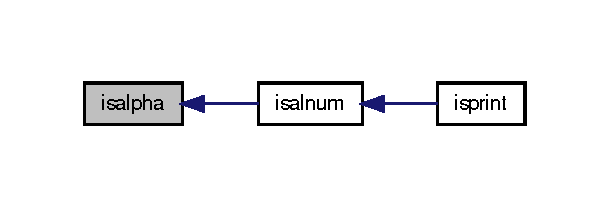
\includegraphics[width=294pt]{ctype_8h_a25908ae63aac2df990634e1ae5bd14d9_icgraph}
\end{center}
\end{figure}


\hypertarget{ctype_8h_aea4929b1b41f1a6d723e0312b1f050ed}{\index{ctype.\-h@{ctype.\-h}!isblank@{isblank}}
\index{isblank@{isblank}!ctype.h@{ctype.\-h}}
\subsubsection[{isblank}]{\setlength{\rightskip}{0pt plus 5cm}int isblank (
\begin{DoxyParamCaption}
\item[{int}]{c}
\end{DoxyParamCaption}
)}}\label{ctype_8h_aea4929b1b41f1a6d723e0312b1f050ed}
Vérifie si le caractère est blanc, c'est-\/à-\/dire un espace ou une tabulation.


\begin{DoxyParams}{Paramètres}
{\em c} & le caractère à vérifier.\\
\hline
\end{DoxyParams}
\begin{DoxyReturn}{Renvoie}
vrai si le caractère est blanc. 
\end{DoxyReturn}
\hypertarget{ctype_8h_a0008a4e8e7889734dc1d83297de07158}{\index{ctype.\-h@{ctype.\-h}!iscntrl@{iscntrl}}
\index{iscntrl@{iscntrl}!ctype.h@{ctype.\-h}}
\subsubsection[{iscntrl}]{\setlength{\rightskip}{0pt plus 5cm}int iscntrl (
\begin{DoxyParamCaption}
\item[{int}]{c}
\end{DoxyParamCaption}
)}}\label{ctype_8h_a0008a4e8e7889734dc1d83297de07158}
Vérifie si l'on a un caractère de contrôle.


\begin{DoxyParams}{Paramètres}
{\em c} & le caractère à vérifier.\\
\hline
\end{DoxyParams}
\begin{DoxyReturn}{Renvoie}
vrai si le caractère est de contrôle. 
\end{DoxyReturn}
\hypertarget{ctype_8h_a3fa45b35c8abf67a950b6d3d4063dede}{\index{ctype.\-h@{ctype.\-h}!isdigit@{isdigit}}
\index{isdigit@{isdigit}!ctype.h@{ctype.\-h}}
\subsubsection[{isdigit}]{\setlength{\rightskip}{0pt plus 5cm}int isdigit (
\begin{DoxyParamCaption}
\item[{int}]{c}
\end{DoxyParamCaption}
)}}\label{ctype_8h_a3fa45b35c8abf67a950b6d3d4063dede}

\begin{DoxyParams}{Paramètres}
{\em c} & le caractère à vérifier.\\
\hline
\end{DoxyParams}
\begin{DoxyReturn}{Renvoie}
vrai si le caractère est un chiffre. 
\end{DoxyReturn}


Voici le graphe des appelants de cette fonction \-:\nopagebreak
\begin{figure}[H]
\begin{center}
\leavevmode
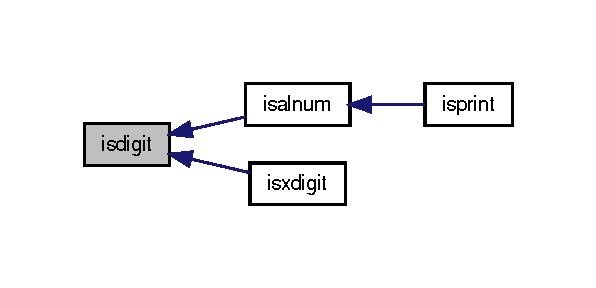
\includegraphics[width=288pt]{ctype_8h_a3fa45b35c8abf67a950b6d3d4063dede_icgraph}
\end{center}
\end{figure}


\hypertarget{ctype_8h_a7b8f652a0423a80922dd89d8829db5f2}{\index{ctype.\-h@{ctype.\-h}!islower@{islower}}
\index{islower@{islower}!ctype.h@{ctype.\-h}}
\subsubsection[{islower}]{\setlength{\rightskip}{0pt plus 5cm}int islower (
\begin{DoxyParamCaption}
\item[{int}]{c}
\end{DoxyParamCaption}
)}}\label{ctype_8h_a7b8f652a0423a80922dd89d8829db5f2}

\begin{DoxyParams}{Paramètres}
{\em c} & le caractère à vérifier.\\
\hline
\end{DoxyParams}
\begin{DoxyReturn}{Renvoie}
vrai si le caractère est minuscule. 
\end{DoxyReturn}


Voici le graphe des appelants de cette fonction \-:\nopagebreak
\begin{figure}[H]
\begin{center}
\leavevmode
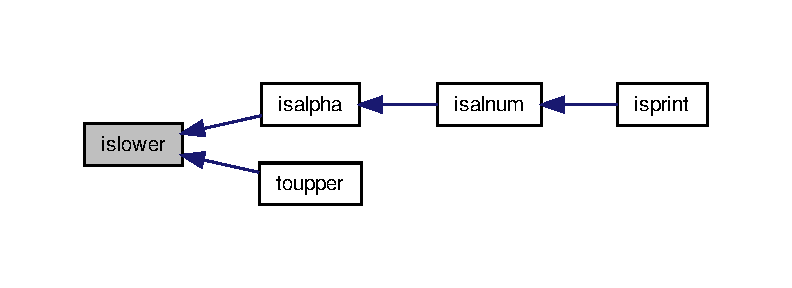
\includegraphics[width=350pt]{ctype_8h_a7b8f652a0423a80922dd89d8829db5f2_icgraph}
\end{center}
\end{figure}


\hypertarget{ctype_8h_a99355d8f0fb41ec43effb95189db0ed4}{\index{ctype.\-h@{ctype.\-h}!isprint@{isprint}}
\index{isprint@{isprint}!ctype.h@{ctype.\-h}}
\subsubsection[{isprint}]{\setlength{\rightskip}{0pt plus 5cm}int isprint (
\begin{DoxyParamCaption}
\item[{int}]{c}
\end{DoxyParamCaption}
)}}\label{ctype_8h_a99355d8f0fb41ec43effb95189db0ed4}

\begin{DoxyParams}{Paramètres}
{\em c} & le caractère à vérifier.\\
\hline
\end{DoxyParams}
\begin{DoxyReturn}{Renvoie}
vrai si le caractère est imprimable. 
\end{DoxyReturn}


Voici le graphe d'appel pour cette fonction \-:\nopagebreak
\begin{figure}[H]
\begin{center}
\leavevmode
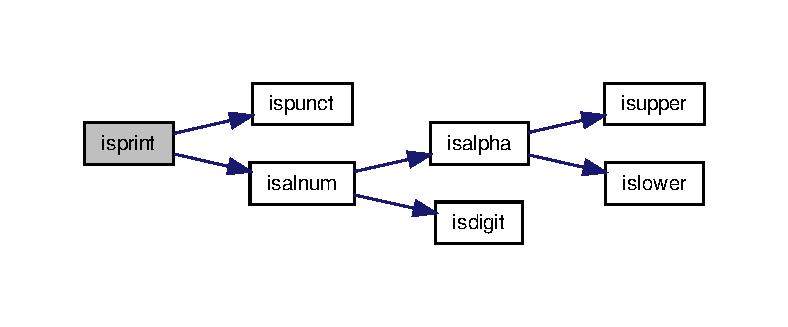
\includegraphics[width=350pt]{ctype_8h_a99355d8f0fb41ec43effb95189db0ed4_cgraph}
\end{center}
\end{figure}


\hypertarget{ctype_8h_af29554b3ec04ea7684482bffed5dbce6}{\index{ctype.\-h@{ctype.\-h}!ispunct@{ispunct}}
\index{ispunct@{ispunct}!ctype.h@{ctype.\-h}}
\subsubsection[{ispunct}]{\setlength{\rightskip}{0pt plus 5cm}int ispunct (
\begin{DoxyParamCaption}
\item[{int}]{c}
\end{DoxyParamCaption}
)}}\label{ctype_8h_af29554b3ec04ea7684482bffed5dbce6}
Vérifie s'il s'agit d'un caractère imprimable, qui ne soit ni un espace, ni un caractère alphanumérique.


\begin{DoxyParams}{Paramètres}
{\em c} & le caractère à vérifier.\\
\hline
\end{DoxyParams}
\begin{DoxyReturn}{Renvoie}
vrai si le caractère est une ponctuation. 
\end{DoxyReturn}


Voici le graphe des appelants de cette fonction \-:\nopagebreak
\begin{figure}[H]
\begin{center}
\leavevmode
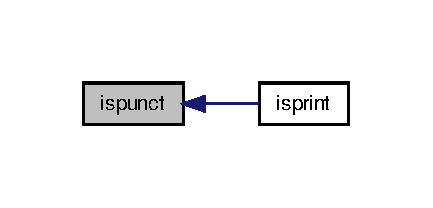
\includegraphics[width=208pt]{ctype_8h_af29554b3ec04ea7684482bffed5dbce6_icgraph}
\end{center}
\end{figure}


\hypertarget{ctype_8h_a56be4166e4673843042a548a7f513dbc}{\index{ctype.\-h@{ctype.\-h}!isspace@{isspace}}
\index{isspace@{isspace}!ctype.h@{ctype.\-h}}
\subsubsection[{isspace}]{\setlength{\rightskip}{0pt plus 5cm}int isspace (
\begin{DoxyParamCaption}
\item[{int}]{c}
\end{DoxyParamCaption}
)}}\label{ctype_8h_a56be4166e4673843042a548a7f513dbc}
Vérifie si l'on a un caractère blanc, d'espacement. Il s'agit de \-: espace, saut de page (form-\/feed, '\textbackslash{}f'), saut de ligne (newline, '\textbackslash{}n'), retour chariot (carriage return, '\textbackslash{}r'), tabulation horizontale ('\textbackslash{}t'), et tabulation verticale ('\textbackslash{}v').


\begin{DoxyParams}{Paramètres}
{\em c} & le caractère à vérifier.\\
\hline
\end{DoxyParams}
\begin{DoxyReturn}{Renvoie}
vrai si le caractère est d'espacement. 
\end{DoxyReturn}
\hypertarget{ctype_8h_adadd6582d46775aab6a51e29d16d9f77}{\index{ctype.\-h@{ctype.\-h}!isupper@{isupper}}
\index{isupper@{isupper}!ctype.h@{ctype.\-h}}
\subsubsection[{isupper}]{\setlength{\rightskip}{0pt plus 5cm}int isupper (
\begin{DoxyParamCaption}
\item[{int}]{c}
\end{DoxyParamCaption}
)}}\label{ctype_8h_adadd6582d46775aab6a51e29d16d9f77}
Vérifie si l'on a un caractère majuscule.


\begin{DoxyParams}{Paramètres}
{\em c} & le caractère à vérifier.\\
\hline
\end{DoxyParams}
\begin{DoxyReturn}{Renvoie}
vrai si le caractère est majuscule. 
\end{DoxyReturn}


Voici le graphe des appelants de cette fonction \-:\nopagebreak
\begin{figure}[H]
\begin{center}
\leavevmode
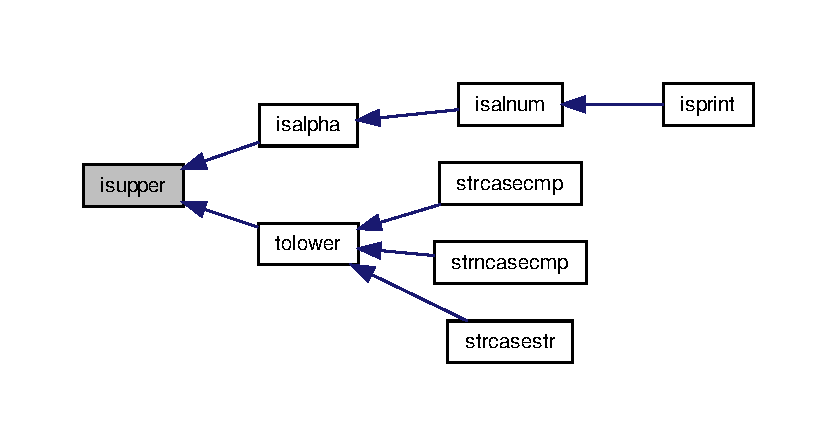
\includegraphics[width=350pt]{ctype_8h_adadd6582d46775aab6a51e29d16d9f77_icgraph}
\end{center}
\end{figure}


\hypertarget{ctype_8h_adaf3aadefe3fc4fb07b6be0d7b880f53}{\index{ctype.\-h@{ctype.\-h}!isxdigit@{isxdigit}}
\index{isxdigit@{isxdigit}!ctype.h@{ctype.\-h}}
\subsubsection[{isxdigit}]{\setlength{\rightskip}{0pt plus 5cm}int isxdigit (
\begin{DoxyParamCaption}
\item[{int}]{c}
\end{DoxyParamCaption}
)}}\label{ctype_8h_adaf3aadefe3fc4fb07b6be0d7b880f53}
Vérifie s'il s'agit d'un chiffre hexadécimal, c'est à dire 0 1 2 3 4 5 6 7 8 9 a b c d e f A B C D E F.


\begin{DoxyParams}{Paramètres}
{\em c} & le caractère à vérifier.\\
\hline
\end{DoxyParams}
\begin{DoxyReturn}{Renvoie}
vrai si le caractère est un chiffre hexadécimal. 
\end{DoxyReturn}


Voici le graphe d'appel pour cette fonction \-:\nopagebreak
\begin{figure}[H]
\begin{center}
\leavevmode
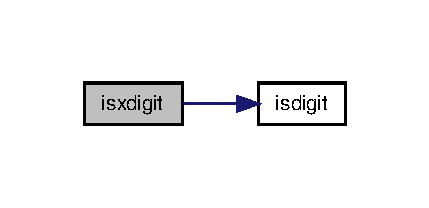
\includegraphics[width=206pt]{ctype_8h_adaf3aadefe3fc4fb07b6be0d7b880f53_cgraph}
\end{center}
\end{figure}


\hypertarget{ctype_8h_ac79d6114c9df7350cedcd8cf921a6ea4}{\index{ctype.\-h@{ctype.\-h}!tolower@{tolower}}
\index{tolower@{tolower}!ctype.h@{ctype.\-h}}
\subsubsection[{tolower}]{\setlength{\rightskip}{0pt plus 5cm}int tolower (
\begin{DoxyParamCaption}
\item[{int}]{c}
\end{DoxyParamCaption}
)}}\label{ctype_8h_ac79d6114c9df7350cedcd8cf921a6ea4}
Convertit la lettre c en minuscule si c'est possible.


\begin{DoxyParams}{Paramètres}
{\em c} & le caractère à convertir.\\
\hline
\end{DoxyParams}
\begin{DoxyReturn}{Renvoie}
le caractère converti. 
\end{DoxyReturn}


Voici le graphe d'appel pour cette fonction \-:\nopagebreak
\begin{figure}[H]
\begin{center}
\leavevmode
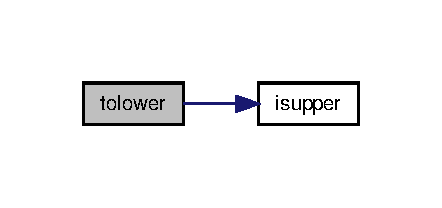
\includegraphics[width=296pt]{ctype_8h_ac79d6114c9df7350cedcd8cf921a6ea4_cgraph}
\end{center}
\end{figure}




Voici le graphe des appelants de cette fonction \-:\nopagebreak
\begin{figure}[H]
\begin{center}
\leavevmode
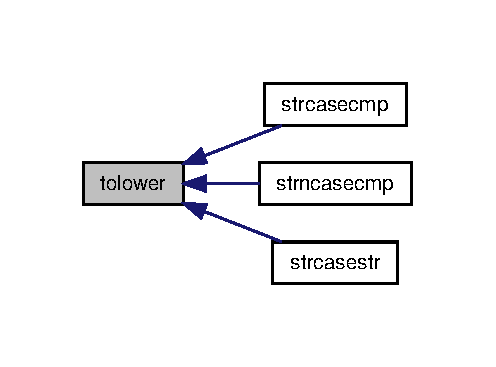
\includegraphics[width=238pt]{ctype_8h_ac79d6114c9df7350cedcd8cf921a6ea4_icgraph}
\end{center}
\end{figure}


\hypertarget{ctype_8h_a9c2f57ac3865af9006fdbfd5db9fd517}{\index{ctype.\-h@{ctype.\-h}!toupper@{toupper}}
\index{toupper@{toupper}!ctype.h@{ctype.\-h}}
\subsubsection[{toupper}]{\setlength{\rightskip}{0pt plus 5cm}int toupper (
\begin{DoxyParamCaption}
\item[{int}]{c}
\end{DoxyParamCaption}
)}}\label{ctype_8h_a9c2f57ac3865af9006fdbfd5db9fd517}
Convertit la lettre c en majuscule si c'est possible.


\begin{DoxyParams}{Paramètres}
{\em c} & le caractère à convertir.\\
\hline
\end{DoxyParams}
\begin{DoxyReturn}{Renvoie}
le caractère converti. 
\end{DoxyReturn}


Voici le graphe d'appel pour cette fonction \-:\nopagebreak
\begin{figure}[H]
\begin{center}
\leavevmode
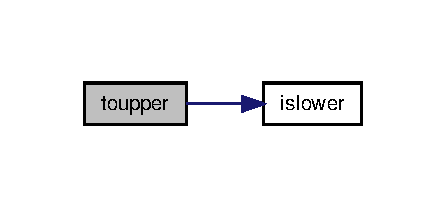
\includegraphics[width=214pt]{ctype_8h_a9c2f57ac3865af9006fdbfd5db9fd517_cgraph}
\end{center}
\end{figure}



\hypertarget{dirent_8h}{\section{Référence du fichier libc/include/dirent.h}
\label{dirent_8h}\index{libc/include/dirent.\-h@{libc/include/dirent.\-h}}
}


Définition de D\-I\-R et struct dirent.  


{\ttfamily \#include $<$sys/cdefs.\-h$>$}\\*
{\ttfamily \#include $<$sys/types.\-h$>$}\\*
{\ttfamily \#include $<$sys/stat.\-h$>$}\\*
Graphe des dépendances par inclusion de dirent.\-h\-:\nopagebreak
\begin{figure}[H]
\begin{center}
\leavevmode
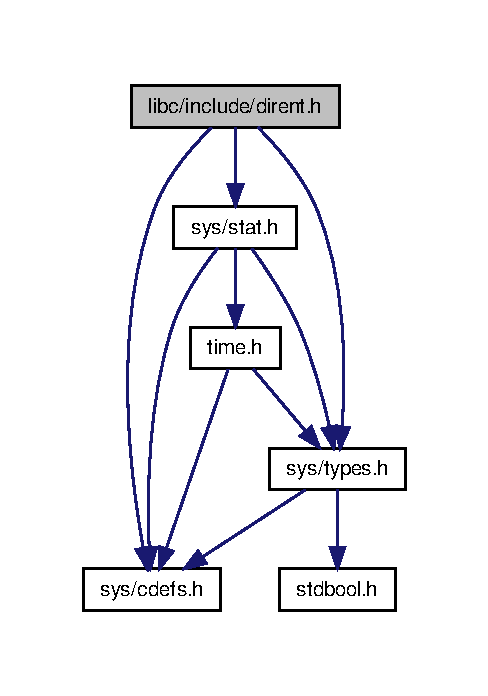
\includegraphics[width=234pt]{dirent_8h__incl}
\end{center}
\end{figure}
Ce graphe montre quels fichiers incluent directement ou indirectement ce fichier \-:\nopagebreak
\begin{figure}[H]
\begin{center}
\leavevmode
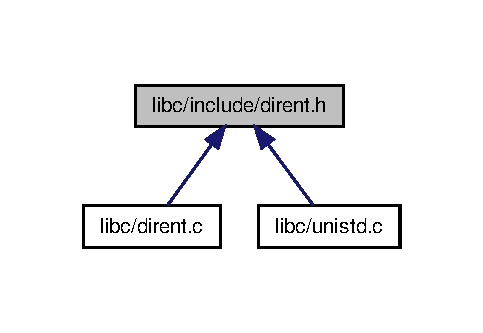
\includegraphics[width=232pt]{dirent_8h__dep__incl}
\end{center}
\end{figure}
\subsection*{Structures de données}
\begin{DoxyCompactItemize}
\item 
struct \hyperlink{struct__DIR}{\-\_\-\-D\-I\-R}
\item 
struct \hyperlink{structdirent}{dirent}
\end{DoxyCompactItemize}
\subsection*{Macros}
\begin{DoxyCompactItemize}
\item 
\#define \hyperlink{dirent_8h_ac64541bdd81c961304b9babef1402640}{N\-A\-M\-E\-\_\-\-M\-A\-X}~256
\end{DoxyCompactItemize}
\subsection*{Définitions de type}
\begin{DoxyCompactItemize}
\item 
typedef struct \hyperlink{struct__DIR}{\-\_\-\-D\-I\-R} \hyperlink{dirent_8h_a9e986c0f8d94ffe9983a6eabb17cbb9a}{D\-I\-R}
\end{DoxyCompactItemize}
\subsection*{Fonctions}
\begin{DoxyCompactItemize}
\item 
int \hyperlink{dirent_8h_aee98bbe743c2d14dbaa67f01c3fb9ed5}{mkdir} (const char $\ast$pathname, \hyperlink{kstat_8h_af8f4385bb42836d1e3ad4fea9d71d1b9}{mode\-\_\-t} \hyperlink{structmode}{mode})
\item 
\hyperlink{dirent_8h_a9e986c0f8d94ffe9983a6eabb17cbb9a}{D\-I\-R} $\ast$ \hyperlink{dirent_8h_ad09dd96447776d2bc5d8321e4b499591}{opendir} (const char $\ast$dirname)
\item 
struct \hyperlink{structdirent}{dirent} $\ast$ \hyperlink{dirent_8h_a58257faf8b13b3f14558613c632b2373}{readdir} (\hyperlink{dirent_8h_a9e986c0f8d94ffe9983a6eabb17cbb9a}{D\-I\-R} $\ast$dirp)
\item 
int \hyperlink{dirent_8h_aaeac2b41e8c2c3a5f91c9bd511a8c0a6}{closedir} (\hyperlink{dirent_8h_a9e986c0f8d94ffe9983a6eabb17cbb9a}{D\-I\-R} $\ast$dirp)
\end{DoxyCompactItemize}


\subsection{Description détaillée}
\begin{DoxyAuthor}{Auteur}
Tac\-O\-S developers
\end{DoxyAuthor}
\hypertarget{wait_8c_LICENSE}{}\subsection{L\-I\-C\-E\-N\-S\-E}\label{wait_8c_LICENSE}
Copyright (C) 2010, 2011, 2012 -\/ Tac\-O\-S developers.

This program is free software; you can redistribute it and/or modify it under the terms of the G\-N\-U General Public License as published by the Free Software Foundation; either version 3 of the License, or (at your option) any later version.

This program is distributed in the hope that it will be useful, but W\-I\-T\-H\-O\-U\-T A\-N\-Y W\-A\-R\-R\-A\-N\-T\-Y; without even the implied warranty of M\-E\-R\-C\-H\-A\-N\-T\-A\-B\-I\-L\-I\-T\-Y or F\-I\-T\-N\-E\-S\-S F\-O\-R A P\-A\-R\-T\-I\-C\-U\-L\-A\-R P\-U\-R\-P\-O\-S\-E. See the G\-N\-U General Public License for more details at \href{http://www.gnu.org/copyleft/gpl.html}{\tt http\-://www.\-gnu.\-org/copyleft/gpl.\-html}

You should have received a copy of the G\-N\-U General Public License along with this program; if not, see \href{http://www.gnu.org/licenses}{\tt http\-://www.\-gnu.\-org/licenses}.\hypertarget{wait_8c_DESCRIPTION}{}\subsection{D\-E\-S\-C\-R\-I\-P\-T\-I\-O\-N}\label{wait_8c_DESCRIPTION}


\subsection{Documentation des macros}
\hypertarget{dirent_8h_ac64541bdd81c961304b9babef1402640}{\index{dirent.\-h@{dirent.\-h}!N\-A\-M\-E\-\_\-\-M\-A\-X@{N\-A\-M\-E\-\_\-\-M\-A\-X}}
\index{N\-A\-M\-E\-\_\-\-M\-A\-X@{N\-A\-M\-E\-\_\-\-M\-A\-X}!dirent.h@{dirent.\-h}}
\subsubsection[{N\-A\-M\-E\-\_\-\-M\-A\-X}]{\setlength{\rightskip}{0pt plus 5cm}\#define N\-A\-M\-E\-\_\-\-M\-A\-X~256}}\label{dirent_8h_ac64541bdd81c961304b9babef1402640}
Taille maximale d'un nom de fichier. 

\subsection{Documentation des définitions de type}
\hypertarget{dirent_8h_a9e986c0f8d94ffe9983a6eabb17cbb9a}{\index{dirent.\-h@{dirent.\-h}!D\-I\-R@{D\-I\-R}}
\index{D\-I\-R@{D\-I\-R}!dirent.h@{dirent.\-h}}
\subsubsection[{D\-I\-R}]{\setlength{\rightskip}{0pt plus 5cm}typedef struct {\bf \-\_\-\-D\-I\-R}  {\bf D\-I\-R}}}\label{dirent_8h_a9e986c0f8d94ffe9983a6eabb17cbb9a}
Structure permettant de lire un dossier. 

\subsection{Documentation des fonctions}
\hypertarget{dirent_8h_aaeac2b41e8c2c3a5f91c9bd511a8c0a6}{\index{dirent.\-h@{dirent.\-h}!closedir@{closedir}}
\index{closedir@{closedir}!dirent.h@{dirent.\-h}}
\subsubsection[{closedir}]{\setlength{\rightskip}{0pt plus 5cm}int closedir (
\begin{DoxyParamCaption}
\item[{{\bf D\-I\-R} $\ast$}]{dirp}
\end{DoxyParamCaption}
)}}\label{dirent_8h_aaeac2b41e8c2c3a5f91c9bd511a8c0a6}
Fermeture d'un dossier ouvert.


\begin{DoxyParams}{Paramètres}
{\em dirp} & La structure D\-I\-R initialisée par opendir.\\
\hline
\end{DoxyParams}
\begin{DoxyReturn}{Renvoie}
0 en cas de succès. 
\end{DoxyReturn}


Voici le graphe d'appel pour cette fonction \-:\nopagebreak
\begin{figure}[H]
\begin{center}
\leavevmode
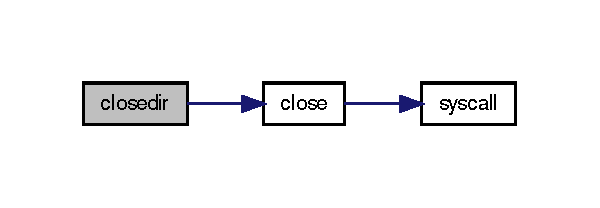
\includegraphics[width=290pt]{dirent_8h_aaeac2b41e8c2c3a5f91c9bd511a8c0a6_cgraph}
\end{center}
\end{figure}


\hypertarget{dirent_8h_aee98bbe743c2d14dbaa67f01c3fb9ed5}{\index{dirent.\-h@{dirent.\-h}!mkdir@{mkdir}}
\index{mkdir@{mkdir}!dirent.h@{dirent.\-h}}
\subsubsection[{mkdir}]{\setlength{\rightskip}{0pt plus 5cm}int mkdir (
\begin{DoxyParamCaption}
\item[{const char $\ast$}]{pathname, }
\item[{{\bf mode\-\_\-t}}]{mode}
\end{DoxyParamCaption}
)}}\label{dirent_8h_aee98bbe743c2d14dbaa67f01c3fb9ed5}
Crée un nouveau répertoire.


\begin{DoxyParams}{Paramètres}
{\em pathname} & Le chemin du dossier à créer. \\
\hline
{\em mode} & Les droits d'accès.\\
\hline
\end{DoxyParams}
\begin{DoxyReturn}{Renvoie}
0 en cas de succès. 
\end{DoxyReturn}


Voici le graphe d'appel pour cette fonction \-:\nopagebreak
\begin{figure}[H]
\begin{center}
\leavevmode
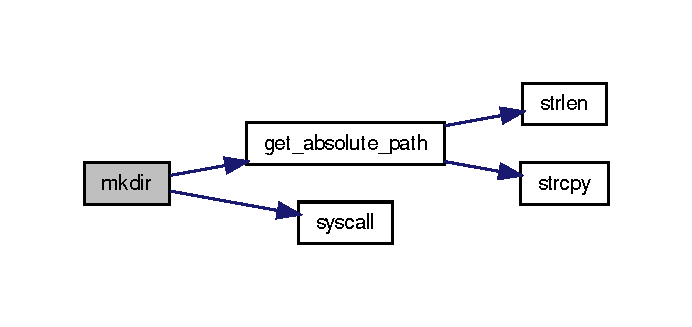
\includegraphics[width=334pt]{dirent_8h_aee98bbe743c2d14dbaa67f01c3fb9ed5_cgraph}
\end{center}
\end{figure}


\hypertarget{dirent_8h_ad09dd96447776d2bc5d8321e4b499591}{\index{dirent.\-h@{dirent.\-h}!opendir@{opendir}}
\index{opendir@{opendir}!dirent.h@{dirent.\-h}}
\subsubsection[{opendir}]{\setlength{\rightskip}{0pt plus 5cm}{\bf D\-I\-R}$\ast$ opendir (
\begin{DoxyParamCaption}
\item[{const char $\ast$}]{dirname}
\end{DoxyParamCaption}
)}}\label{dirent_8h_ad09dd96447776d2bc5d8321e4b499591}
Ouvre un dossier pour lister les fichiers à l'intérieur.


\begin{DoxyParams}{Paramètres}
{\em dirname} & Le chemin du dossier à ouvrir.\\
\hline
\end{DoxyParams}
\begin{DoxyReturn}{Renvoie}
Une structure D\-I\-R permettant de lire le contenu du dossier. 
\end{DoxyReturn}


Voici le graphe d'appel pour cette fonction \-:\nopagebreak
\begin{figure}[H]
\begin{center}
\leavevmode
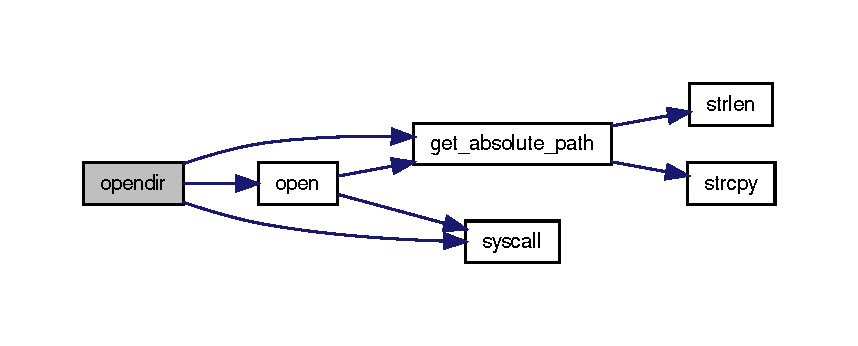
\includegraphics[width=350pt]{dirent_8h_ad09dd96447776d2bc5d8321e4b499591_cgraph}
\end{center}
\end{figure}




Voici le graphe des appelants de cette fonction \-:\nopagebreak
\begin{figure}[H]
\begin{center}
\leavevmode
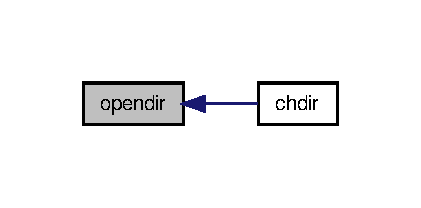
\includegraphics[width=202pt]{dirent_8h_ad09dd96447776d2bc5d8321e4b499591_icgraph}
\end{center}
\end{figure}


\hypertarget{dirent_8h_a58257faf8b13b3f14558613c632b2373}{\index{dirent.\-h@{dirent.\-h}!readdir@{readdir}}
\index{readdir@{readdir}!dirent.h@{dirent.\-h}}
\subsubsection[{readdir}]{\setlength{\rightskip}{0pt plus 5cm}struct {\bf dirent}$\ast$ readdir (
\begin{DoxyParamCaption}
\item[{{\bf D\-I\-R} $\ast$}]{dirp}
\end{DoxyParamCaption}
)\hspace{0.3cm}{\ttfamily [read]}}}\label{dirent_8h_a58257faf8b13b3f14558613c632b2373}
Lecture de la prochaine entrée du dossier.


\begin{DoxyParams}{Paramètres}
{\em dirp} & La structure D\-I\-R initialisée par opendir.\\
\hline
\end{DoxyParams}
\begin{DoxyReturn}{Renvoie}
Un directory entry. 
\end{DoxyReturn}


Voici le graphe d'appel pour cette fonction \-:\nopagebreak
\begin{figure}[H]
\begin{center}
\leavevmode
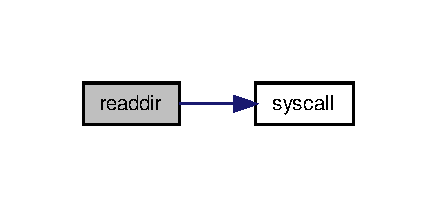
\includegraphics[width=210pt]{dirent_8h_a58257faf8b13b3f14558613c632b2373_cgraph}
\end{center}
\end{figure}



\hypertarget{errno_8h}{\section{\-Référence du fichier libc/include/errno.h}
\label{errno_8h}\index{libc/include/errno.\-h@{libc/include/errno.\-h}}
}
{\ttfamily \#include $<$sys/cdefs.\-h$>$}\*
\-Graphe des dépendances par inclusion de errno.\-h\-:\nopagebreak
\begin{figure}[H]
\begin{center}
\leavevmode
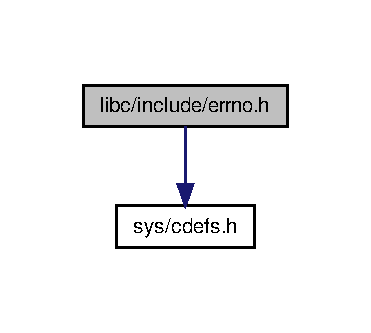
\includegraphics[width=178pt]{errno_8h__incl}
\end{center}
\end{figure}
\-Ce graphe montre quels fichiers incluent directement ou indirectement ce fichier \-:\nopagebreak
\begin{figure}[H]
\begin{center}
\leavevmode
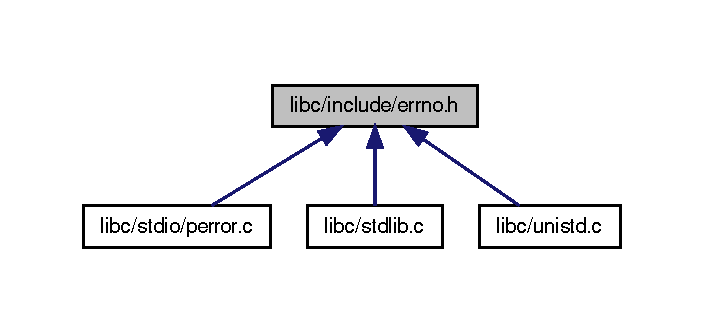
\includegraphics[width=338pt]{errno_8h__dep__incl}
\end{center}
\end{figure}
\subsection*{\-Macros}
\begin{DoxyCompactItemize}
\item 
\#define \hyperlink{errno_8h_af0fac1cea1165b4debec7f686edf3313}{\-E\-A\-G\-A\-I\-N}~1
\item 
\#define \hyperlink{errno_8h_ac54507d66b43ad12f9356257323c0018}{\-E\-B\-A\-D\-F}~2
\item 
\#define \hyperlink{errno_8h_a3f317946e043623f9d6b93dbf60e6316}{\-E\-F\-A\-U\-L\-T}~3
\item 
\#define \hyperlink{errno_8h_af5401a500939ed1812c04ca200b95eef}{\-E\-F\-B\-I\-G}~4
\item 
\#define \hyperlink{errno_8h_a46b83d9f6c23b1b65a8cecfd775ddaed}{\-E\-I\-N\-T\-R}~5
\item 
\#define \hyperlink{errno_8h_a2d1678d5a7cc8ce499643f3b8957def4}{\-E\-I\-N\-V\-A\-L}~6
\item 
\#define \hyperlink{errno_8h_a70979f50f9c83e5aebab3d6a1bd4cf35}{\-E\-I\-O}~7
\item 
\#define \hyperlink{errno_8h_a088abe8bad2df798edad3053d719b937}{\-E\-N\-O\-S\-P\-C}~8
\item 
\#define \hyperlink{errno_8h_a5f8d33deb08fa27c04897b278ac7f965}{\-E\-P\-I\-P\-E}~9
\item 
\#define \hyperlink{errno_8h_aa1591a4f3a86360108de5b9ba34980ca}{\-E\-R\-A\-N\-G\-E}~10
\item 
\#define \hyperlink{errno_8h_a03e689f378f643d16ea7537918528a48}{\-E\-N\-O\-E\-N\-T}~11
\item 
\#define \hyperlink{errno_8h_a9262fb92f7ef662d0bdd577912a5b101}{\-E\-N\-O\-T\-D\-I\-R}~12
\item 
\#define \hyperlink{errno_8h_a0a3bef9e5c47e42917692b5dae3b5498}{\-E\-E\-X\-I\-S\-T}~13
\item 
\#define \hyperlink{errno_8h_add669d31505a077f769cff8e66c780b3}{\-E\-P\-E\-R\-M}~14
\item 
\#define \hyperlink{errno_8h_ae22c3a1e0a38f3896de238cc30d0e19b}{\-E\-I\-S\-D\-I\-R}~15
\item 
\#define \hyperlink{errno_8h_a5554094b3fb4bb6ebeb0157cb3f82a55}{\-E\-N\-F\-I\-L\-E}~16
\item 
\#define \hyperlink{errno_8h_a64a75c174882ddbfa726c7fd040f87a1}{\-E\-M\-F\-I\-L\-E}~17
\end{DoxyCompactItemize}
\subsection*{\-Variables}
\begin{DoxyCompactItemize}
\item 
const char $\ast$ \hyperlink{errno_8h_a76ebfe24a40210e5935998c1fa86d3a0}{sys\-\_\-errlist} \mbox{[}$\,$\mbox{]}
\item 
int \hyperlink{errno_8h_ad65a8842cc674e3ddf69355898c0ecbf}{errno}
\end{DoxyCompactItemize}


\subsection{\-Description détaillée}
\begin{DoxyAuthor}{\-Auteur}
\-Tac\-O\-S developers
\end{DoxyAuthor}
\hypertarget{wait_8c_LICENSE}{}\subsection{\-L\-I\-C\-E\-N\-S\-E}\label{wait_8c_LICENSE}
\-Copyright (\-C) 2010, 2011, 2012 -\/ \-Tac\-O\-S developers.

\-This program is free software; you can redistribute it and/or modify it under the terms of the \-G\-N\-U \-General \-Public \-License as published by the \-Free \-Software \-Foundation; either version 3 of the \-License, or (at your option) any later version.

\-This program is distributed in the hope that it will be useful, but \-W\-I\-T\-H\-O\-U\-T \-A\-N\-Y \-W\-A\-R\-R\-A\-N\-T\-Y; without even the implied warranty of \-M\-E\-R\-C\-H\-A\-N\-T\-A\-B\-I\-L\-I\-T\-Y or \-F\-I\-T\-N\-E\-S\-S \-F\-O\-R \-A \-P\-A\-R\-T\-I\-C\-U\-L\-A\-R \-P\-U\-R\-P\-O\-S\-E. \-See the \-G\-N\-U \-General \-Public \-License for more details at \href{http://www.gnu.org/copyleft/gpl.html}{\tt http\-://www.\-gnu.\-org/copyleft/gpl.\-html}

\-You should have received a copy of the \-G\-N\-U \-General \-Public \-License along with this program; if not, see $<$\href{http://www.gnu.org/licenses}{\tt http\-://www.\-gnu.\-org/licenses}$>$.\hypertarget{wait_8c_DESCRIPTION}{}\subsection{\-D\-E\-S\-C\-R\-I\-P\-T\-I\-O\-N}\label{wait_8c_DESCRIPTION}
\-Description de ce que fait le fichier 

\subsection{\-Documentation des macros}
\hypertarget{errno_8h_af0fac1cea1165b4debec7f686edf3313}{\index{errno.\-h@{errno.\-h}!\-E\-A\-G\-A\-I\-N@{\-E\-A\-G\-A\-I\-N}}
\index{\-E\-A\-G\-A\-I\-N@{\-E\-A\-G\-A\-I\-N}!errno.h@{errno.\-h}}
\subsubsection[{\-E\-A\-G\-A\-I\-N}]{\setlength{\rightskip}{0pt plus 5cm}\#define {\bf \-E\-A\-G\-A\-I\-N}~1}}\label{errno_8h_af0fac1cea1165b4debec7f686edf3313}
\-Essai encore ;). \hypertarget{errno_8h_ac54507d66b43ad12f9356257323c0018}{\index{errno.\-h@{errno.\-h}!\-E\-B\-A\-D\-F@{\-E\-B\-A\-D\-F}}
\index{\-E\-B\-A\-D\-F@{\-E\-B\-A\-D\-F}!errno.h@{errno.\-h}}
\subsubsection[{\-E\-B\-A\-D\-F}]{\setlength{\rightskip}{0pt plus 5cm}\#define {\bf \-E\-B\-A\-D\-F}~2}}\label{errno_8h_ac54507d66b43ad12f9356257323c0018}
\-Mauvais numero de fichier. \hypertarget{errno_8h_a0a3bef9e5c47e42917692b5dae3b5498}{\index{errno.\-h@{errno.\-h}!\-E\-E\-X\-I\-S\-T@{\-E\-E\-X\-I\-S\-T}}
\index{\-E\-E\-X\-I\-S\-T@{\-E\-E\-X\-I\-S\-T}!errno.h@{errno.\-h}}
\subsubsection[{\-E\-E\-X\-I\-S\-T}]{\setlength{\rightskip}{0pt plus 5cm}\#define {\bf \-E\-E\-X\-I\-S\-T}~13}}\label{errno_8h_a0a3bef9e5c47e42917692b5dae3b5498}
existe déjà. \hypertarget{errno_8h_a3f317946e043623f9d6b93dbf60e6316}{\index{errno.\-h@{errno.\-h}!\-E\-F\-A\-U\-L\-T@{\-E\-F\-A\-U\-L\-T}}
\index{\-E\-F\-A\-U\-L\-T@{\-E\-F\-A\-U\-L\-T}!errno.h@{errno.\-h}}
\subsubsection[{\-E\-F\-A\-U\-L\-T}]{\setlength{\rightskip}{0pt plus 5cm}\#define {\bf \-E\-F\-A\-U\-L\-T}~3}}\label{errno_8h_a3f317946e043623f9d6b93dbf60e6316}
\-Mauvaise adresse. \hypertarget{errno_8h_af5401a500939ed1812c04ca200b95eef}{\index{errno.\-h@{errno.\-h}!\-E\-F\-B\-I\-G@{\-E\-F\-B\-I\-G}}
\index{\-E\-F\-B\-I\-G@{\-E\-F\-B\-I\-G}!errno.h@{errno.\-h}}
\subsubsection[{\-E\-F\-B\-I\-G}]{\setlength{\rightskip}{0pt plus 5cm}\#define {\bf \-E\-F\-B\-I\-G}~4}}\label{errno_8h_af5401a500939ed1812c04ca200b95eef}
\-Fichier trop gros. \hypertarget{errno_8h_a46b83d9f6c23b1b65a8cecfd775ddaed}{\index{errno.\-h@{errno.\-h}!\-E\-I\-N\-T\-R@{\-E\-I\-N\-T\-R}}
\index{\-E\-I\-N\-T\-R@{\-E\-I\-N\-T\-R}!errno.h@{errno.\-h}}
\subsubsection[{\-E\-I\-N\-T\-R}]{\setlength{\rightskip}{0pt plus 5cm}\#define {\bf \-E\-I\-N\-T\-R}~5}}\label{errno_8h_a46b83d9f6c23b1b65a8cecfd775ddaed}
\-System call interrompu. \hypertarget{errno_8h_a2d1678d5a7cc8ce499643f3b8957def4}{\index{errno.\-h@{errno.\-h}!\-E\-I\-N\-V\-A\-L@{\-E\-I\-N\-V\-A\-L}}
\index{\-E\-I\-N\-V\-A\-L@{\-E\-I\-N\-V\-A\-L}!errno.h@{errno.\-h}}
\subsubsection[{\-E\-I\-N\-V\-A\-L}]{\setlength{\rightskip}{0pt plus 5cm}\#define {\bf \-E\-I\-N\-V\-A\-L}~6}}\label{errno_8h_a2d1678d5a7cc8ce499643f3b8957def4}
\-Argument invalide. \hypertarget{errno_8h_a70979f50f9c83e5aebab3d6a1bd4cf35}{\index{errno.\-h@{errno.\-h}!\-E\-I\-O@{\-E\-I\-O}}
\index{\-E\-I\-O@{\-E\-I\-O}!errno.h@{errno.\-h}}
\subsubsection[{\-E\-I\-O}]{\setlength{\rightskip}{0pt plus 5cm}\#define {\bf \-E\-I\-O}~7}}\label{errno_8h_a70979f50f9c83e5aebab3d6a1bd4cf35}
\-Erreur d'entrée / sortie. \hypertarget{errno_8h_ae22c3a1e0a38f3896de238cc30d0e19b}{\index{errno.\-h@{errno.\-h}!\-E\-I\-S\-D\-I\-R@{\-E\-I\-S\-D\-I\-R}}
\index{\-E\-I\-S\-D\-I\-R@{\-E\-I\-S\-D\-I\-R}!errno.h@{errno.\-h}}
\subsubsection[{\-E\-I\-S\-D\-I\-R}]{\setlength{\rightskip}{0pt plus 5cm}\#define {\bf \-E\-I\-S\-D\-I\-R}~15}}\label{errno_8h_ae22c3a1e0a38f3896de238cc30d0e19b}
c'est un dossier. \hypertarget{errno_8h_a64a75c174882ddbfa726c7fd040f87a1}{\index{errno.\-h@{errno.\-h}!\-E\-M\-F\-I\-L\-E@{\-E\-M\-F\-I\-L\-E}}
\index{\-E\-M\-F\-I\-L\-E@{\-E\-M\-F\-I\-L\-E}!errno.h@{errno.\-h}}
\subsubsection[{\-E\-M\-F\-I\-L\-E}]{\setlength{\rightskip}{0pt plus 5cm}\#define {\bf \-E\-M\-F\-I\-L\-E}~17}}\label{errno_8h_a64a75c174882ddbfa726c7fd040f87a1}
\-Trop de fichiers ouverts. \hypertarget{errno_8h_a5554094b3fb4bb6ebeb0157cb3f82a55}{\index{errno.\-h@{errno.\-h}!\-E\-N\-F\-I\-L\-E@{\-E\-N\-F\-I\-L\-E}}
\index{\-E\-N\-F\-I\-L\-E@{\-E\-N\-F\-I\-L\-E}!errno.h@{errno.\-h}}
\subsubsection[{\-E\-N\-F\-I\-L\-E}]{\setlength{\rightskip}{0pt plus 5cm}\#define {\bf \-E\-N\-F\-I\-L\-E}~16}}\label{errno_8h_a5554094b3fb4bb6ebeb0157cb3f82a55}
\-Overflow de la file table. \hypertarget{errno_8h_a03e689f378f643d16ea7537918528a48}{\index{errno.\-h@{errno.\-h}!\-E\-N\-O\-E\-N\-T@{\-E\-N\-O\-E\-N\-T}}
\index{\-E\-N\-O\-E\-N\-T@{\-E\-N\-O\-E\-N\-T}!errno.h@{errno.\-h}}
\subsubsection[{\-E\-N\-O\-E\-N\-T}]{\setlength{\rightskip}{0pt plus 5cm}\#define {\bf \-E\-N\-O\-E\-N\-T}~11}}\label{errno_8h_a03e689f378f643d16ea7537918528a48}
entrée non trouvée. \hypertarget{errno_8h_a088abe8bad2df798edad3053d719b937}{\index{errno.\-h@{errno.\-h}!\-E\-N\-O\-S\-P\-C@{\-E\-N\-O\-S\-P\-C}}
\index{\-E\-N\-O\-S\-P\-C@{\-E\-N\-O\-S\-P\-C}!errno.h@{errno.\-h}}
\subsubsection[{\-E\-N\-O\-S\-P\-C}]{\setlength{\rightskip}{0pt plus 5cm}\#define {\bf \-E\-N\-O\-S\-P\-C}~8}}\label{errno_8h_a088abe8bad2df798edad3053d719b937}
\-Plus d'espace libre. \hypertarget{errno_8h_a9262fb92f7ef662d0bdd577912a5b101}{\index{errno.\-h@{errno.\-h}!\-E\-N\-O\-T\-D\-I\-R@{\-E\-N\-O\-T\-D\-I\-R}}
\index{\-E\-N\-O\-T\-D\-I\-R@{\-E\-N\-O\-T\-D\-I\-R}!errno.h@{errno.\-h}}
\subsubsection[{\-E\-N\-O\-T\-D\-I\-R}]{\setlength{\rightskip}{0pt plus 5cm}\#define {\bf \-E\-N\-O\-T\-D\-I\-R}~12}}\label{errno_8h_a9262fb92f7ef662d0bdd577912a5b101}
ce n'est pas un dossier. \hypertarget{errno_8h_add669d31505a077f769cff8e66c780b3}{\index{errno.\-h@{errno.\-h}!\-E\-P\-E\-R\-M@{\-E\-P\-E\-R\-M}}
\index{\-E\-P\-E\-R\-M@{\-E\-P\-E\-R\-M}!errno.h@{errno.\-h}}
\subsubsection[{\-E\-P\-E\-R\-M}]{\setlength{\rightskip}{0pt plus 5cm}\#define {\bf \-E\-P\-E\-R\-M}~14}}\label{errno_8h_add669d31505a077f769cff8e66c780b3}
operation non permise. \hypertarget{errno_8h_a5f8d33deb08fa27c04897b278ac7f965}{\index{errno.\-h@{errno.\-h}!\-E\-P\-I\-P\-E@{\-E\-P\-I\-P\-E}}
\index{\-E\-P\-I\-P\-E@{\-E\-P\-I\-P\-E}!errno.h@{errno.\-h}}
\subsubsection[{\-E\-P\-I\-P\-E}]{\setlength{\rightskip}{0pt plus 5cm}\#define {\bf \-E\-P\-I\-P\-E}~9}}\label{errno_8h_a5f8d33deb08fa27c04897b278ac7f965}
broken pipe. \hypertarget{errno_8h_aa1591a4f3a86360108de5b9ba34980ca}{\index{errno.\-h@{errno.\-h}!\-E\-R\-A\-N\-G\-E@{\-E\-R\-A\-N\-G\-E}}
\index{\-E\-R\-A\-N\-G\-E@{\-E\-R\-A\-N\-G\-E}!errno.h@{errno.\-h}}
\subsubsection[{\-E\-R\-A\-N\-G\-E}]{\setlength{\rightskip}{0pt plus 5cm}\#define {\bf \-E\-R\-A\-N\-G\-E}~10}}\label{errno_8h_aa1591a4f3a86360108de5b9ba34980ca}
\-Résultat maths non representable. 

\subsection{\-Documentation des variables}
\hypertarget{errno_8h_ad65a8842cc674e3ddf69355898c0ecbf}{\index{errno.\-h@{errno.\-h}!errno@{errno}}
\index{errno@{errno}!errno.h@{errno.\-h}}
\subsubsection[{errno}]{\setlength{\rightskip}{0pt plus 5cm}int {\bf errno}}}\label{errno_8h_ad65a8842cc674e3ddf69355898c0ecbf}
\-Variable qui contient le numéro de la dernière erreur. \hypertarget{errno_8h_a76ebfe24a40210e5935998c1fa86d3a0}{\index{errno.\-h@{errno.\-h}!sys\-\_\-errlist@{sys\-\_\-errlist}}
\index{sys\-\_\-errlist@{sys\-\_\-errlist}!errno.h@{errno.\-h}}
\subsubsection[{sys\-\_\-errlist}]{\setlength{\rightskip}{0pt plus 5cm}const char$\ast$ {\bf sys\-\_\-errlist}\mbox{[}$\,$\mbox{]}}}\label{errno_8h_a76ebfe24a40210e5935998c1fa86d3a0}
\-Liste des messages d'erreur. 
\hypertarget{fcntl_8h}{\section{Référence du fichier libc/include/fcntl.h}
\label{fcntl_8h}\index{libc/include/fcntl.\-h@{libc/include/fcntl.\-h}}
}


File control operations.  


{\ttfamily \#include $<$sys/cdefs.\-h$>$}\\*
Graphe des dépendances par inclusion de fcntl.\-h\-:\nopagebreak
\begin{figure}[H]
\begin{center}
\leavevmode
\includegraphics[width=174pt]{fcntl_8h__incl}
\end{center}
\end{figure}
Ce graphe montre quels fichiers incluent directement ou indirectement ce fichier \-:\nopagebreak
\begin{figure}[H]
\begin{center}
\leavevmode
\includegraphics[width=350pt]{fcntl_8h__dep__incl}
\end{center}
\end{figure}
\subsection*{Macros}
\begin{DoxyCompactItemize}
\item 
\#define \hyperlink{fcntl_8h_a4dc4d45e07d2abc899bcaf04b2846a87}{O\-\_\-\-A\-C\-C\-M\-O\-D\-E}~00000003
\item 
\#define \hyperlink{fcntl_8h_a7a68c9ffaac7dbcd652225dd7c06a54b}{O\-\_\-\-R\-D\-O\-N\-L\-Y}~00000000
\item 
\#define \hyperlink{fcntl_8h_a11b644a8526139c4cc1850dac1271ced}{O\-\_\-\-W\-R\-O\-N\-L\-Y}~00000001
\item 
\#define \hyperlink{fcntl_8h_abb0586253488ee61072b73557eeb873b}{O\-\_\-\-R\-D\-W\-R}~00000002
\item 
\#define \hyperlink{fcntl_8h_a1cf6b1de1fffedaa1d26b189e9a8d2cc}{O\-\_\-\-C\-R\-E\-A\-T}~00000100
\item 
\hypertarget{fcntl_8h_a9f5acfe79fafe14b6694447bd0e9f10b}{\#define {\bfseries O\-\_\-\-E\-X\-C\-L}~00000200 /$\ast$ not \hyperlink{fcntl_8h_a5752d6571b615f1b7b1b0f719c2bc69d}{fcntl} $\ast$/}\label{fcntl_8h_a9f5acfe79fafe14b6694447bd0e9f10b}

\item 
\hypertarget{fcntl_8h_a2e375ab32c7ef4581b026be28e4cc116}{\#define {\bfseries O\-\_\-\-N\-O\-C\-T\-T\-Y}~00000400 /$\ast$ not \hyperlink{fcntl_8h_a5752d6571b615f1b7b1b0f719c2bc69d}{fcntl} $\ast$/}\label{fcntl_8h_a2e375ab32c7ef4581b026be28e4cc116}

\item 
\#define \hyperlink{fcntl_8h_ad1d67e453fb3031f40f8cd3403773813}{O\-\_\-\-T\-R\-U\-N\-C}~00001000
\item 
\#define \hyperlink{fcntl_8h_ae036f789407d21f07b211552d67b3214}{O\-\_\-\-A\-P\-P\-E\-N\-D}~00002000
\item 
\#define \hyperlink{fcntl_8h_a39d33ce33804efd4d52606d59071c6d8}{O\-\_\-\-N\-O\-N\-B\-L\-O\-C\-K}~00004000
\item 
\#define \hyperlink{fcntl_8h_aae85139bfa94236d126bb1e3b772998f}{O\-\_\-\-S\-Y\-N\-C}~00010000
\item 
\hypertarget{fcntl_8h_a1c28a43c30721462ad7e40f37051c9ca}{\#define {\bfseries F\-A\-S\-Y\-N\-C}~00020000 /$\ast$ \hyperlink{fcntl_8h_a5752d6571b615f1b7b1b0f719c2bc69d}{fcntl}, for B\-S\-D compatibility $\ast$/}\label{fcntl_8h_a1c28a43c30721462ad7e40f37051c9ca}

\item 
\#define \hyperlink{fcntl_8h_ad28ccbf6f0a42c91c160ac5ada0c8429}{O\-\_\-\-D\-I\-R\-E\-C\-T}~00040000
\item 
\#define \hyperlink{fcntl_8h_a6afd3dd2f570069804b40e6aa24fc966}{O\-\_\-\-D\-I\-R\-E\-C\-T\-O\-R\-Y}~00200000
\item 
\#define \hyperlink{fcntl_8h_a82d4d551b214905742c9e045185d352a}{O\-\_\-\-N\-O\-F\-O\-L\-L\-O\-W}~00400000
\item 
\hypertarget{fcntl_8h_a476bb0c47c4ceb1669c15c2635c94300}{\#define {\bfseries O\-\_\-\-N\-O\-A\-T\-I\-M\-E}~01000000}\label{fcntl_8h_a476bb0c47c4ceb1669c15c2635c94300}

\item 
\#define \hyperlink{fcntl_8h_ad6d8fbe4e494b4dbe051612572d3f757}{O\-\_\-\-C\-L\-O\-E\-X\-E\-C}~02000000
\item 
\hypertarget{fcntl_8h_af2939853c650561d3495ed40f68f6249}{\#define {\bfseries F\-\_\-\-S\-E\-T\-F\-L}~4}\label{fcntl_8h_af2939853c650561d3495ed40f68f6249}

\item 
\hypertarget{fcntl_8h_a025fad21a889c79f02ec53abe3526c32}{\#define {\bfseries F\-\_\-\-G\-E\-T\-F\-L}~5}\label{fcntl_8h_a025fad21a889c79f02ec53abe3526c32}

\end{DoxyCompactItemize}
\subsection*{Fonctions}
\begin{DoxyCompactItemize}
\item 
int \hyperlink{fcntl_8h_adcb60598073f6f9cbb0091ef6768fa5c}{open} (const char $\ast$pathname, int flags)
\item 
int \hyperlink{fcntl_8h_ae68e7e3d0b126184d5d00e78e94305fb}{close} (int id)
\item 
int \hyperlink{fcntl_8h_a5752d6571b615f1b7b1b0f719c2bc69d}{fcntl} (int fd, unsigned int request, void $\ast$data)
\end{DoxyCompactItemize}


\subsection{Description détaillée}
\begin{DoxyAuthor}{Auteur}
Tac\-O\-S developers
\end{DoxyAuthor}
\hypertarget{wait_8c_LICENSE}{}\subsection{L\-I\-C\-E\-N\-S\-E}\label{wait_8c_LICENSE}
Copyright (C) 2010, 2011, 2012 -\/ Tac\-O\-S developers.

This program is free software; you can redistribute it and/or modify it under the terms of the G\-N\-U General Public License as published by the Free Software Foundation; either version 3 of the License, or (at your option) any later version.

This program is distributed in the hope that it will be useful, but W\-I\-T\-H\-O\-U\-T A\-N\-Y W\-A\-R\-R\-A\-N\-T\-Y; without even the implied warranty of M\-E\-R\-C\-H\-A\-N\-T\-A\-B\-I\-L\-I\-T\-Y or F\-I\-T\-N\-E\-S\-S F\-O\-R A P\-A\-R\-T\-I\-C\-U\-L\-A\-R P\-U\-R\-P\-O\-S\-E. See the G\-N\-U General Public License for more details at \href{http://www.gnu.org/copyleft/gpl.html}{\tt http\-://www.\-gnu.\-org/copyleft/gpl.\-html}

You should have received a copy of the G\-N\-U General Public License along with this program; if not, see \href{http://www.gnu.org/licenses}{\tt http\-://www.\-gnu.\-org/licenses}.\hypertarget{wait_8c_DESCRIPTION}{}\subsection{D\-E\-S\-C\-R\-I\-P\-T\-I\-O\-N}\label{wait_8c_DESCRIPTION}


\subsection{Documentation des macros}
\hypertarget{fcntl_8h_a4dc4d45e07d2abc899bcaf04b2846a87}{\index{fcntl.\-h@{fcntl.\-h}!O\-\_\-\-A\-C\-C\-M\-O\-D\-E@{O\-\_\-\-A\-C\-C\-M\-O\-D\-E}}
\index{O\-\_\-\-A\-C\-C\-M\-O\-D\-E@{O\-\_\-\-A\-C\-C\-M\-O\-D\-E}!fcntl.h@{fcntl.\-h}}
\subsubsection[{O\-\_\-\-A\-C\-C\-M\-O\-D\-E}]{\setlength{\rightskip}{0pt plus 5cm}\#define O\-\_\-\-A\-C\-C\-M\-O\-D\-E~00000003}}\label{fcntl_8h_a4dc4d45e07d2abc899bcaf04b2846a87}
Access mode mask. \hypertarget{fcntl_8h_ae036f789407d21f07b211552d67b3214}{\index{fcntl.\-h@{fcntl.\-h}!O\-\_\-\-A\-P\-P\-E\-N\-D@{O\-\_\-\-A\-P\-P\-E\-N\-D}}
\index{O\-\_\-\-A\-P\-P\-E\-N\-D@{O\-\_\-\-A\-P\-P\-E\-N\-D}!fcntl.h@{fcntl.\-h}}
\subsubsection[{O\-\_\-\-A\-P\-P\-E\-N\-D}]{\setlength{\rightskip}{0pt plus 5cm}\#define O\-\_\-\-A\-P\-P\-E\-N\-D~00002000}}\label{fcntl_8h_ae036f789407d21f07b211552d67b3214}
Ajoute en fin de fichier. \hypertarget{fcntl_8h_ad6d8fbe4e494b4dbe051612572d3f757}{\index{fcntl.\-h@{fcntl.\-h}!O\-\_\-\-C\-L\-O\-E\-X\-E\-C@{O\-\_\-\-C\-L\-O\-E\-X\-E\-C}}
\index{O\-\_\-\-C\-L\-O\-E\-X\-E\-C@{O\-\_\-\-C\-L\-O\-E\-X\-E\-C}!fcntl.h@{fcntl.\-h}}
\subsubsection[{O\-\_\-\-C\-L\-O\-E\-X\-E\-C}]{\setlength{\rightskip}{0pt plus 5cm}\#define O\-\_\-\-C\-L\-O\-E\-X\-E\-C~02000000}}\label{fcntl_8h_ad6d8fbe4e494b4dbe051612572d3f757}
set close\-\_\-on\-\_\-exec \hypertarget{fcntl_8h_a1cf6b1de1fffedaa1d26b189e9a8d2cc}{\index{fcntl.\-h@{fcntl.\-h}!O\-\_\-\-C\-R\-E\-A\-T@{O\-\_\-\-C\-R\-E\-A\-T}}
\index{O\-\_\-\-C\-R\-E\-A\-T@{O\-\_\-\-C\-R\-E\-A\-T}!fcntl.h@{fcntl.\-h}}
\subsubsection[{O\-\_\-\-C\-R\-E\-A\-T}]{\setlength{\rightskip}{0pt plus 5cm}\#define O\-\_\-\-C\-R\-E\-A\-T~00000100}}\label{fcntl_8h_a1cf6b1de1fffedaa1d26b189e9a8d2cc}
Create file if non-\/existant. \hypertarget{fcntl_8h_ad28ccbf6f0a42c91c160ac5ada0c8429}{\index{fcntl.\-h@{fcntl.\-h}!O\-\_\-\-D\-I\-R\-E\-C\-T@{O\-\_\-\-D\-I\-R\-E\-C\-T}}
\index{O\-\_\-\-D\-I\-R\-E\-C\-T@{O\-\_\-\-D\-I\-R\-E\-C\-T}!fcntl.h@{fcntl.\-h}}
\subsubsection[{O\-\_\-\-D\-I\-R\-E\-C\-T}]{\setlength{\rightskip}{0pt plus 5cm}\#define O\-\_\-\-D\-I\-R\-E\-C\-T~00040000}}\label{fcntl_8h_ad28ccbf6f0a42c91c160ac5ada0c8429}
direct disk access hint \hypertarget{fcntl_8h_a6afd3dd2f570069804b40e6aa24fc966}{\index{fcntl.\-h@{fcntl.\-h}!O\-\_\-\-D\-I\-R\-E\-C\-T\-O\-R\-Y@{O\-\_\-\-D\-I\-R\-E\-C\-T\-O\-R\-Y}}
\index{O\-\_\-\-D\-I\-R\-E\-C\-T\-O\-R\-Y@{O\-\_\-\-D\-I\-R\-E\-C\-T\-O\-R\-Y}!fcntl.h@{fcntl.\-h}}
\subsubsection[{O\-\_\-\-D\-I\-R\-E\-C\-T\-O\-R\-Y}]{\setlength{\rightskip}{0pt plus 5cm}\#define O\-\_\-\-D\-I\-R\-E\-C\-T\-O\-R\-Y~00200000}}\label{fcntl_8h_a6afd3dd2f570069804b40e6aa24fc966}
must be a directory \hypertarget{fcntl_8h_a82d4d551b214905742c9e045185d352a}{\index{fcntl.\-h@{fcntl.\-h}!O\-\_\-\-N\-O\-F\-O\-L\-L\-O\-W@{O\-\_\-\-N\-O\-F\-O\-L\-L\-O\-W}}
\index{O\-\_\-\-N\-O\-F\-O\-L\-L\-O\-W@{O\-\_\-\-N\-O\-F\-O\-L\-L\-O\-W}!fcntl.h@{fcntl.\-h}}
\subsubsection[{O\-\_\-\-N\-O\-F\-O\-L\-L\-O\-W}]{\setlength{\rightskip}{0pt plus 5cm}\#define O\-\_\-\-N\-O\-F\-O\-L\-L\-O\-W~00400000}}\label{fcntl_8h_a82d4d551b214905742c9e045185d352a}
don't follow links \hypertarget{fcntl_8h_a39d33ce33804efd4d52606d59071c6d8}{\index{fcntl.\-h@{fcntl.\-h}!O\-\_\-\-N\-O\-N\-B\-L\-O\-C\-K@{O\-\_\-\-N\-O\-N\-B\-L\-O\-C\-K}}
\index{O\-\_\-\-N\-O\-N\-B\-L\-O\-C\-K@{O\-\_\-\-N\-O\-N\-B\-L\-O\-C\-K}!fcntl.h@{fcntl.\-h}}
\subsubsection[{O\-\_\-\-N\-O\-N\-B\-L\-O\-C\-K}]{\setlength{\rightskip}{0pt plus 5cm}\#define O\-\_\-\-N\-O\-N\-B\-L\-O\-C\-K~00004000}}\label{fcntl_8h_a39d33ce33804efd4d52606d59071c6d8}
Le read ne sera pas bloquant. \hypertarget{fcntl_8h_a7a68c9ffaac7dbcd652225dd7c06a54b}{\index{fcntl.\-h@{fcntl.\-h}!O\-\_\-\-R\-D\-O\-N\-L\-Y@{O\-\_\-\-R\-D\-O\-N\-L\-Y}}
\index{O\-\_\-\-R\-D\-O\-N\-L\-Y@{O\-\_\-\-R\-D\-O\-N\-L\-Y}!fcntl.h@{fcntl.\-h}}
\subsubsection[{O\-\_\-\-R\-D\-O\-N\-L\-Y}]{\setlength{\rightskip}{0pt plus 5cm}\#define O\-\_\-\-R\-D\-O\-N\-L\-Y~00000000}}\label{fcntl_8h_a7a68c9ffaac7dbcd652225dd7c06a54b}
Open file for read only access. \hypertarget{fcntl_8h_abb0586253488ee61072b73557eeb873b}{\index{fcntl.\-h@{fcntl.\-h}!O\-\_\-\-R\-D\-W\-R@{O\-\_\-\-R\-D\-W\-R}}
\index{O\-\_\-\-R\-D\-W\-R@{O\-\_\-\-R\-D\-W\-R}!fcntl.h@{fcntl.\-h}}
\subsubsection[{O\-\_\-\-R\-D\-W\-R}]{\setlength{\rightskip}{0pt plus 5cm}\#define O\-\_\-\-R\-D\-W\-R~00000002}}\label{fcntl_8h_abb0586253488ee61072b73557eeb873b}
Open file for both reading and writing. \hypertarget{fcntl_8h_aae85139bfa94236d126bb1e3b772998f}{\index{fcntl.\-h@{fcntl.\-h}!O\-\_\-\-S\-Y\-N\-C@{O\-\_\-\-S\-Y\-N\-C}}
\index{O\-\_\-\-S\-Y\-N\-C@{O\-\_\-\-S\-Y\-N\-C}!fcntl.h@{fcntl.\-h}}
\subsubsection[{O\-\_\-\-S\-Y\-N\-C}]{\setlength{\rightskip}{0pt plus 5cm}\#define O\-\_\-\-S\-Y\-N\-C~00010000}}\label{fcntl_8h_aae85139bfa94236d126bb1e3b772998f}
Appel à write bloquant tant que les données ne sont pas écrites physiquement sur le disque. \hypertarget{fcntl_8h_ad1d67e453fb3031f40f8cd3403773813}{\index{fcntl.\-h@{fcntl.\-h}!O\-\_\-\-T\-R\-U\-N\-C@{O\-\_\-\-T\-R\-U\-N\-C}}
\index{O\-\_\-\-T\-R\-U\-N\-C@{O\-\_\-\-T\-R\-U\-N\-C}!fcntl.h@{fcntl.\-h}}
\subsubsection[{O\-\_\-\-T\-R\-U\-N\-C}]{\setlength{\rightskip}{0pt plus 5cm}\#define O\-\_\-\-T\-R\-U\-N\-C~00001000}}\label{fcntl_8h_ad1d67e453fb3031f40f8cd3403773813}
Tronque le fichier à une longueur nulle. \hypertarget{fcntl_8h_a11b644a8526139c4cc1850dac1271ced}{\index{fcntl.\-h@{fcntl.\-h}!O\-\_\-\-W\-R\-O\-N\-L\-Y@{O\-\_\-\-W\-R\-O\-N\-L\-Y}}
\index{O\-\_\-\-W\-R\-O\-N\-L\-Y@{O\-\_\-\-W\-R\-O\-N\-L\-Y}!fcntl.h@{fcntl.\-h}}
\subsubsection[{O\-\_\-\-W\-R\-O\-N\-L\-Y}]{\setlength{\rightskip}{0pt plus 5cm}\#define O\-\_\-\-W\-R\-O\-N\-L\-Y~00000001}}\label{fcntl_8h_a11b644a8526139c4cc1850dac1271ced}
Open file for write only access. 

\subsection{Documentation des fonctions}
\hypertarget{fcntl_8h_ae68e7e3d0b126184d5d00e78e94305fb}{\index{fcntl.\-h@{fcntl.\-h}!close@{close}}
\index{close@{close}!fcntl.h@{fcntl.\-h}}
\subsubsection[{close}]{\setlength{\rightskip}{0pt plus 5cm}int close (
\begin{DoxyParamCaption}
\item[{int}]{id}
\end{DoxyParamCaption}
)}}\label{fcntl_8h_ae68e7e3d0b126184d5d00e78e94305fb}
Ferme un fichier ouvert.


\begin{DoxyParams}{Paramètres}
{\em id} & descripteur du fichier.\\
\hline
\end{DoxyParams}
\begin{DoxyReturn}{Renvoie}
0 en cas de succès. 
\end{DoxyReturn}


Voici le graphe d'appel pour cette fonction \-:\nopagebreak
\begin{figure}[H]
\begin{center}
\leavevmode
\includegraphics[width=202pt]{fcntl_8h_ae68e7e3d0b126184d5d00e78e94305fb_cgraph}
\end{center}
\end{figure}




Voici le graphe des appelants de cette fonction \-:\nopagebreak
\begin{figure}[H]
\begin{center}
\leavevmode
\includegraphics[width=206pt]{fcntl_8h_ae68e7e3d0b126184d5d00e78e94305fb_icgraph}
\end{center}
\end{figure}


\hypertarget{fcntl_8h_a5752d6571b615f1b7b1b0f719c2bc69d}{\index{fcntl.\-h@{fcntl.\-h}!fcntl@{fcntl}}
\index{fcntl@{fcntl}!fcntl.h@{fcntl.\-h}}
\subsubsection[{fcntl}]{\setlength{\rightskip}{0pt plus 5cm}int fcntl (
\begin{DoxyParamCaption}
\item[{int}]{fd, }
\item[{unsigned int}]{request, }
\item[{void $\ast$}]{data}
\end{DoxyParamCaption}
)}}\label{fcntl_8h_a5752d6571b615f1b7b1b0f719c2bc69d}
Manipulation d'un descripteur de fichier.


\begin{DoxyParams}{Paramètres}
{\em fd} & descripteur du fichier. \\
\hline
{\em request} & action à faire. \\
\hline
{\em data} & les arguments nécessaires à l'action.\\
\hline
\end{DoxyParams}
\begin{DoxyReturn}{Renvoie}
valeur en fonction de l'action. 
\end{DoxyReturn}


Voici le graphe d'appel pour cette fonction \-:\nopagebreak
\begin{figure}[H]
\begin{center}
\leavevmode
\includegraphics[width=198pt]{fcntl_8h_a5752d6571b615f1b7b1b0f719c2bc69d_cgraph}
\end{center}
\end{figure}


\hypertarget{fcntl_8h_adcb60598073f6f9cbb0091ef6768fa5c}{\index{fcntl.\-h@{fcntl.\-h}!open@{open}}
\index{open@{open}!fcntl.h@{fcntl.\-h}}
\subsubsection[{open}]{\setlength{\rightskip}{0pt plus 5cm}int open (
\begin{DoxyParamCaption}
\item[{const char $\ast$}]{pathname, }
\item[{int}]{flags}
\end{DoxyParamCaption}
)}}\label{fcntl_8h_adcb60598073f6f9cbb0091ef6768fa5c}
Ouvrir un fichier ou un périphérique.


\begin{DoxyParams}{Paramètres}
{\em pathname} & Chemin du fichier. \\
\hline
{\em flags} & Flags pour indiquer le mode d'ouverture.\\
\hline
\end{DoxyParams}
\begin{DoxyReturn}{Renvoie}
l'id du file descriptor. -\/1 en cas d'erreur. 
\end{DoxyReturn}


Voici le graphe d'appel pour cette fonction \-:\nopagebreak
\begin{figure}[H]
\begin{center}
\leavevmode
\includegraphics[width=328pt]{fcntl_8h_adcb60598073f6f9cbb0091ef6768fa5c_cgraph}
\end{center}
\end{figure}




Voici le graphe des appelants de cette fonction \-:\nopagebreak
\begin{figure}[H]
\begin{center}
\leavevmode
\includegraphics[width=276pt]{fcntl_8h_adcb60598073f6f9cbb0091ef6768fa5c_icgraph}
\end{center}
\end{figure}



\hypertarget{fopen_8h}{\section{Référence du fichier libc/include/fopen.h}
\label{fopen_8h}\index{libc/include/fopen.\-h@{libc/include/fopen.\-h}}
}
{\ttfamily \#include $<$sys/cdefs.\-h$>$}\\*
Graphe des dépendances par inclusion de fopen.\-h\-:\nopagebreak
\begin{figure}[H]
\begin{center}
\leavevmode
\includegraphics[width=180pt]{fopen_8h__incl}
\end{center}
\end{figure}
Ce graphe montre quels fichiers incluent directement ou indirectement ce fichier \-:\nopagebreak
\begin{figure}[H]
\begin{center}
\leavevmode
\includegraphics[width=192pt]{fopen_8h__dep__incl}
\end{center}
\end{figure}
\subsection*{Fonctions}
\begin{DoxyCompactItemize}
\item 
int \hyperlink{fopen_8h_acdefa543c661333e27beda1c868e6ce9}{convert\-\_\-flags} (const char $\ast$\hyperlink{structmode}{mode})
\begin{DoxyCompactList}\small\item\em Conversion de modes de lecture/ecriture/ajout... \end{DoxyCompactList}\end{DoxyCompactItemize}


\subsection{Description détaillée}
\begin{DoxyAuthor}{Auteur}
Tac\-O\-S developers
\end{DoxyAuthor}
\hypertarget{wait_8c_LICENSE}{}\subsection{L\-I\-C\-E\-N\-S\-E}\label{wait_8c_LICENSE}
Copyright (C) 2010, 2011, 2012 -\/ Tac\-O\-S developers.

This program is free software; you can redistribute it and/or modify it under the terms of the G\-N\-U General Public License as published by the Free Software Foundation; either version 3 of the License, or (at your option) any later version.

This program is distributed in the hope that it will be useful, but W\-I\-T\-H\-O\-U\-T A\-N\-Y W\-A\-R\-R\-A\-N\-T\-Y; without even the implied warranty of M\-E\-R\-C\-H\-A\-N\-T\-A\-B\-I\-L\-I\-T\-Y or F\-I\-T\-N\-E\-S\-S F\-O\-R A P\-A\-R\-T\-I\-C\-U\-L\-A\-R P\-U\-R\-P\-O\-S\-E. See the G\-N\-U General Public License for more details at \href{http://www.gnu.org/copyleft/gpl.html}{\tt http\-://www.\-gnu.\-org/copyleft/gpl.\-html}

You should have received a copy of the G\-N\-U General Public License along with this program; if not, see \href{http://www.gnu.org/licenses}{\tt http\-://www.\-gnu.\-org/licenses}.\hypertarget{wait_8c_DESCRIPTION}{}\subsection{D\-E\-S\-C\-R\-I\-P\-T\-I\-O\-N}\label{wait_8c_DESCRIPTION}
Description de ce que fait le fichier

\subsection{Documentation des fonctions}
\hypertarget{fopen_8h_acdefa543c661333e27beda1c868e6ce9}{\index{fopen.\-h@{fopen.\-h}!convert\-\_\-flags@{convert\-\_\-flags}}
\index{convert\-\_\-flags@{convert\-\_\-flags}!fopen.h@{fopen.\-h}}
\subsubsection[{convert\-\_\-flags}]{\setlength{\rightskip}{0pt plus 5cm}int convert\-\_\-flags (
\begin{DoxyParamCaption}
\item[{const char $\ast$}]{mode}
\end{DoxyParamCaption}
)}}\label{fopen_8h_acdefa543c661333e27beda1c868e6ce9}
Converti depuis la forme \char`\"{}r+\char`\"{} par exemple en un entier formé de la superposition de plusieurs masques.


\begin{DoxyParams}{Paramètres}
{\em mode} & le mode présenté sous la forme d'une chaine de caractère.\\
\hline
\end{DoxyParams}
\begin{DoxyReturn}{Renvoie}
un entier contenant les mêmes informations. 
\end{DoxyReturn}


Voici le graphe d'appel pour cette fonction \-:\nopagebreak
\begin{figure}[H]
\begin{center}
\leavevmode
\includegraphics[width=238pt]{fopen_8h_acdefa543c661333e27beda1c868e6ce9_cgraph}
\end{center}
\end{figure}



\hypertarget{libio_8h}{\section{Référence du fichier libc/include/libio.h}
\label{libio_8h}\index{libc/include/libio.\-h@{libc/include/libio.\-h}}
}
{\ttfamily \#include $<$sys/cdefs.\-h$>$}\\*
{\ttfamily \#include $<$sys/types.\-h$>$}\\*
Graphe des dépendances par inclusion de libio.\-h\-:\nopagebreak
\begin{figure}[H]
\begin{center}
\leavevmode
\includegraphics[width=220pt]{libio_8h__incl}
\end{center}
\end{figure}
Ce graphe montre quels fichiers incluent directement ou indirectement ce fichier \-:\nopagebreak
\begin{figure}[H]
\begin{center}
\leavevmode
\includegraphics[width=350pt]{libio_8h__dep__incl}
\end{center}
\end{figure}
\subsection*{Structures de données}
\begin{DoxyCompactItemize}
\item 
struct \hyperlink{struct__IO__FILE}{\-\_\-\-I\-O\-\_\-\-F\-I\-L\-E}
\begin{DoxyCompactList}\small\item\em Gestion de stream. Inspiré de posix. \end{DoxyCompactList}\end{DoxyCompactItemize}
\subsection*{Macros}
\begin{DoxyCompactItemize}
\item 
\#define \hyperlink{libio_8h_a8a7b4be44019ecd4f5daa590b49bfa46}{\-\_\-\-I\-O\-\_\-\-M\-A\-G\-I\-C}~0x\-F\-B\-A\-D0000
\item 
\#define \hyperlink{libio_8h_a5607bcef18c9bfdca76e5e267bfe6cd9}{\-\_\-\-I\-O\-\_\-\-M\-A\-G\-I\-C\-\_\-\-M\-A\-S\-K}~0x\-F\-F\-F\-F0000
\item 
\#define \hyperlink{libio_8h_aecd47314dd69a1e4fc63ada7eff1175b}{\-\_\-\-I\-O\-\_\-\-U\-N\-B\-U\-F\-F\-E\-R\-E\-D}~2
\item 
\#define \hyperlink{libio_8h_ae5debdcd9d593da3bfa82b0727a5f0a6}{\-\_\-\-I\-O\-\_\-\-L\-I\-N\-E\-\_\-\-B\-U\-F}~0x200
\item 
\hypertarget{libio_8h_af7444f32c50ad6356ea75f4b08bb9ab5}{\#define {\bfseries \-\_\-\-I\-O\-\_\-\-E\-O\-F\-\_\-\-S\-E\-E\-N}~0x10}\label{libio_8h_af7444f32c50ad6356ea75f4b08bb9ab5}

\item 
\hypertarget{libio_8h_a1357ee693d9e41c447a1ff3821872abd}{\#define {\bfseries \-\_\-\-I\-O\-\_\-\-E\-R\-R\-\_\-\-S\-E\-E\-N}~0x20}\label{libio_8h_a1357ee693d9e41c447a1ff3821872abd}

\end{DoxyCompactItemize}
\subsection*{Définitions de type}
\begin{DoxyCompactItemize}
\item 
\hypertarget{libio_8h_a912af5ab9f8a52ddd387b7defc0b49f1}{typedef struct \hyperlink{struct__IO__FILE}{\-\_\-\-I\-O\-\_\-\-F\-I\-L\-E} {\bfseries F\-I\-L\-E}}\label{libio_8h_a912af5ab9f8a52ddd387b7defc0b49f1}

\end{DoxyCompactItemize}
\subsection*{Variables}
\begin{DoxyCompactItemize}
\item 
\hyperlink{struct__IO__FILE}{F\-I\-L\-E} $\ast$ \hyperlink{libio_8h_acab9c1fe2a80b10e01858bda28a04244}{stdin}
\item 
\hyperlink{struct__IO__FILE}{F\-I\-L\-E} $\ast$ \hyperlink{libio_8h_ac80f4484175bf6c48d7b7ca4e9897ae6}{stdout}
\item 
\hyperlink{struct__IO__FILE}{F\-I\-L\-E} $\ast$ \hyperlink{libio_8h_ac9e47c346a25e2e7edd2c9b4ca5d0262}{stderr}
\end{DoxyCompactItemize}


\subsection{Description détaillée}
\begin{DoxyAuthor}{Auteur}
Tac\-O\-S developers
\end{DoxyAuthor}
\hypertarget{wait_8c_LICENSE}{}\subsection{L\-I\-C\-E\-N\-S\-E}\label{wait_8c_LICENSE}
Copyright (C) 2010, 2011, 2012 -\/ Tac\-O\-S developers.

This program is free software; you can redistribute it and/or modify it under the terms of the G\-N\-U General Public License as published by the Free Software Foundation; either version 3 of the License, or (at your option) any later version.

This program is distributed in the hope that it will be useful, but W\-I\-T\-H\-O\-U\-T A\-N\-Y W\-A\-R\-R\-A\-N\-T\-Y; without even the implied warranty of M\-E\-R\-C\-H\-A\-N\-T\-A\-B\-I\-L\-I\-T\-Y or F\-I\-T\-N\-E\-S\-S F\-O\-R A P\-A\-R\-T\-I\-C\-U\-L\-A\-R P\-U\-R\-P\-O\-S\-E. See the G\-N\-U General Public License for more details at \href{http://www.gnu.org/copyleft/gpl.html}{\tt http\-://www.\-gnu.\-org/copyleft/gpl.\-html}

You should have received a copy of the G\-N\-U General Public License along with this program; if not, see \href{http://www.gnu.org/licenses}{\tt http\-://www.\-gnu.\-org/licenses}.\hypertarget{wait_8c_DESCRIPTION}{}\subsection{D\-E\-S\-C\-R\-I\-P\-T\-I\-O\-N}\label{wait_8c_DESCRIPTION}
Description de ce que fait le fichier 

\subsection{Documentation des macros}
\hypertarget{libio_8h_ae5debdcd9d593da3bfa82b0727a5f0a6}{\index{libio.\-h@{libio.\-h}!\-\_\-\-I\-O\-\_\-\-L\-I\-N\-E\-\_\-\-B\-U\-F@{\-\_\-\-I\-O\-\_\-\-L\-I\-N\-E\-\_\-\-B\-U\-F}}
\index{\-\_\-\-I\-O\-\_\-\-L\-I\-N\-E\-\_\-\-B\-U\-F@{\-\_\-\-I\-O\-\_\-\-L\-I\-N\-E\-\_\-\-B\-U\-F}!libio.h@{libio.\-h}}
\subsubsection[{\-\_\-\-I\-O\-\_\-\-L\-I\-N\-E\-\_\-\-B\-U\-F}]{\setlength{\rightskip}{0pt plus 5cm}\#define \-\_\-\-I\-O\-\_\-\-L\-I\-N\-E\-\_\-\-B\-U\-F~0x200}}\label{libio_8h_ae5debdcd9d593da3bfa82b0727a5f0a6}
Buffer flushé par une nouvelle ligne. \hypertarget{libio_8h_a8a7b4be44019ecd4f5daa590b49bfa46}{\index{libio.\-h@{libio.\-h}!\-\_\-\-I\-O\-\_\-\-M\-A\-G\-I\-C@{\-\_\-\-I\-O\-\_\-\-M\-A\-G\-I\-C}}
\index{\-\_\-\-I\-O\-\_\-\-M\-A\-G\-I\-C@{\-\_\-\-I\-O\-\_\-\-M\-A\-G\-I\-C}!libio.h@{libio.\-h}}
\subsubsection[{\-\_\-\-I\-O\-\_\-\-M\-A\-G\-I\-C}]{\setlength{\rightskip}{0pt plus 5cm}\#define \-\_\-\-I\-O\-\_\-\-M\-A\-G\-I\-C~0x\-F\-B\-A\-D0000}}\label{libio_8h_a8a7b4be44019ecd4f5daa590b49bfa46}
Magic number (je le garde par compatibilité) \hypertarget{libio_8h_a5607bcef18c9bfdca76e5e267bfe6cd9}{\index{libio.\-h@{libio.\-h}!\-\_\-\-I\-O\-\_\-\-M\-A\-G\-I\-C\-\_\-\-M\-A\-S\-K@{\-\_\-\-I\-O\-\_\-\-M\-A\-G\-I\-C\-\_\-\-M\-A\-S\-K}}
\index{\-\_\-\-I\-O\-\_\-\-M\-A\-G\-I\-C\-\_\-\-M\-A\-S\-K@{\-\_\-\-I\-O\-\_\-\-M\-A\-G\-I\-C\-\_\-\-M\-A\-S\-K}!libio.h@{libio.\-h}}
\subsubsection[{\-\_\-\-I\-O\-\_\-\-M\-A\-G\-I\-C\-\_\-\-M\-A\-S\-K}]{\setlength{\rightskip}{0pt plus 5cm}\#define \-\_\-\-I\-O\-\_\-\-M\-A\-G\-I\-C\-\_\-\-M\-A\-S\-K~0x\-F\-F\-F\-F0000}}\label{libio_8h_a5607bcef18c9bfdca76e5e267bfe6cd9}
Pour filtrer le magic number \hypertarget{libio_8h_aecd47314dd69a1e4fc63ada7eff1175b}{\index{libio.\-h@{libio.\-h}!\-\_\-\-I\-O\-\_\-\-U\-N\-B\-U\-F\-F\-E\-R\-E\-D@{\-\_\-\-I\-O\-\_\-\-U\-N\-B\-U\-F\-F\-E\-R\-E\-D}}
\index{\-\_\-\-I\-O\-\_\-\-U\-N\-B\-U\-F\-F\-E\-R\-E\-D@{\-\_\-\-I\-O\-\_\-\-U\-N\-B\-U\-F\-F\-E\-R\-E\-D}!libio.h@{libio.\-h}}
\subsubsection[{\-\_\-\-I\-O\-\_\-\-U\-N\-B\-U\-F\-F\-E\-R\-E\-D}]{\setlength{\rightskip}{0pt plus 5cm}\#define \-\_\-\-I\-O\-\_\-\-U\-N\-B\-U\-F\-F\-E\-R\-E\-D~2}}\label{libio_8h_aecd47314dd69a1e4fc63ada7eff1175b}
Pas de buffer. 

\subsection{Documentation des variables}
\hypertarget{libio_8h_ac9e47c346a25e2e7edd2c9b4ca5d0262}{\index{libio.\-h@{libio.\-h}!stderr@{stderr}}
\index{stderr@{stderr}!libio.h@{libio.\-h}}
\subsubsection[{stderr}]{\setlength{\rightskip}{0pt plus 5cm}{\bf F\-I\-L\-E}$\ast$ stderr}}\label{libio_8h_ac9e47c346a25e2e7edd2c9b4ca5d0262}
Sortie d'erreur. \hypertarget{libio_8h_acab9c1fe2a80b10e01858bda28a04244}{\index{libio.\-h@{libio.\-h}!stdin@{stdin}}
\index{stdin@{stdin}!libio.h@{libio.\-h}}
\subsubsection[{stdin}]{\setlength{\rightskip}{0pt plus 5cm}{\bf F\-I\-L\-E}$\ast$ stdin}}\label{libio_8h_acab9c1fe2a80b10e01858bda28a04244}
Entrée standard. \hypertarget{libio_8h_ac80f4484175bf6c48d7b7ca4e9897ae6}{\index{libio.\-h@{libio.\-h}!stdout@{stdout}}
\index{stdout@{stdout}!libio.h@{libio.\-h}}
\subsubsection[{stdout}]{\setlength{\rightskip}{0pt plus 5cm}{\bf F\-I\-L\-E}$\ast$ stdout}}\label{libio_8h_ac80f4484175bf6c48d7b7ca4e9897ae6}
Sortie standard. 
\hypertarget{limits_8h}{\section{Référence du fichier kernel/include/klibc/limits.h}
\label{limits_8h}\index{kernel/include/klibc/limits.\-h@{kernel/include/klibc/limits.\-h}}
}


Valeurs extrèmes pour les types de base.  


Ce graphe montre quels fichiers incluent directement ou indirectement ce fichier \-:\nopagebreak
\begin{figure}[H]
\begin{center}
\leavevmode
\includegraphics[width=180pt]{limits_8h__dep__incl}
\end{center}
\end{figure}
\subsection*{Macros}
\begin{DoxyCompactItemize}
\item 
\#define \hyperlink{limits_8h_a308d9dd2c0028ddb184b455bbd7865de}{C\-H\-A\-R\-\_\-\-B\-I\-T}~8
\item 
\#define \hyperlink{limits_8h_a9ec306f36d50c7375e74f0d1c55a3a67}{I\-N\-T\-\_\-\-M\-A\-X}~2147483647
\item 
\#define \hyperlink{limits_8h_a21658776274b3d146c674318b635a334}{I\-N\-T\-\_\-\-M\-I\-N}~(-\/\hyperlink{limits_8h_a9ec306f36d50c7375e74f0d1c55a3a67}{I\-N\-T\-\_\-\-M\-A\-X} -\/ 1)
\item 
\#define \hyperlink{limits_8h_ac998ea02fbd821fc123d60445ce76f38}{U\-I\-N\-T\-\_\-\-M\-A\-X}~4294967295\-U
\item 
\#define \hyperlink{limits_8h_a50fece4db74f09568b2938db583c5655}{L\-O\-N\-G\-\_\-\-M\-A\-X}~2147483647\-L
\item 
\#define \hyperlink{limits_8h_ae8a44c5a7436466221e0f3859d02420f}{L\-O\-N\-G\-\_\-\-M\-I\-N}~(-\/\hyperlink{limits_8h_a50fece4db74f09568b2938db583c5655}{L\-O\-N\-G\-\_\-\-M\-A\-X} -\/ 1\-L)
\end{DoxyCompactItemize}


\subsection{Description détaillée}
\begin{DoxyAuthor}{Auteur}
Tac\-O\-S developers
\end{DoxyAuthor}
\hypertarget{vmm_8c_LICENSE}{}\subsection{L\-I\-C\-E\-N\-S\-E}\label{vmm_8c_LICENSE}
Copyright (C) 2010, 2011, 2012 -\/ Tac\-O\-S developers.

This program is free software; you can redistribute it and/or modify it under the terms of the G\-N\-U General Public License as published by the Free Software Foundation; either version 3 of the License, or (at your option) any later version.

This program is distributed in the hope that it will be useful, but W\-I\-T\-H\-O\-U\-T A\-N\-Y W\-A\-R\-R\-A\-N\-T\-Y; without even the implied warranty of M\-E\-R\-C\-H\-A\-N\-T\-A\-B\-I\-L\-I\-T\-Y or F\-I\-T\-N\-E\-S\-S F\-O\-R A P\-A\-R\-T\-I\-C\-U\-L\-A\-R P\-U\-R\-P\-O\-S\-E. See the G\-N\-U General Public License for more details at \href{http://www.gnu.org/copyleft/gpl.html}{\tt http\-://www.\-gnu.\-org/copyleft/gpl.\-html}

You should have received a copy of the G\-N\-U General Public License along with this program; if not, see \href{http://www.gnu.org/licenses}{\tt http\-://www.\-gnu.\-org/licenses}.\hypertarget{vmm_8c_DESCRIPTION}{}\subsection{D\-E\-S\-C\-R\-I\-P\-T\-I\-O\-N}\label{vmm_8c_DESCRIPTION}


\subsection{Documentation des macros}
\hypertarget{limits_8h_a308d9dd2c0028ddb184b455bbd7865de}{\index{limits.\-h@{limits.\-h}!C\-H\-A\-R\-\_\-\-B\-I\-T@{C\-H\-A\-R\-\_\-\-B\-I\-T}}
\index{C\-H\-A\-R\-\_\-\-B\-I\-T@{C\-H\-A\-R\-\_\-\-B\-I\-T}!limits.h@{limits.\-h}}
\subsubsection[{C\-H\-A\-R\-\_\-\-B\-I\-T}]{\setlength{\rightskip}{0pt plus 5cm}\#define C\-H\-A\-R\-\_\-\-B\-I\-T~8}}\label{limits_8h_a308d9dd2c0028ddb184b455bbd7865de}
Nombre de bits pour un char. \hypertarget{limits_8h_a9ec306f36d50c7375e74f0d1c55a3a67}{\index{limits.\-h@{limits.\-h}!I\-N\-T\-\_\-\-M\-A\-X@{I\-N\-T\-\_\-\-M\-A\-X}}
\index{I\-N\-T\-\_\-\-M\-A\-X@{I\-N\-T\-\_\-\-M\-A\-X}!limits.h@{limits.\-h}}
\subsubsection[{I\-N\-T\-\_\-\-M\-A\-X}]{\setlength{\rightskip}{0pt plus 5cm}\#define I\-N\-T\-\_\-\-M\-A\-X~2147483647}}\label{limits_8h_a9ec306f36d50c7375e74f0d1c55a3a67}
Valeur maximale d'un int signé. \hypertarget{limits_8h_a21658776274b3d146c674318b635a334}{\index{limits.\-h@{limits.\-h}!I\-N\-T\-\_\-\-M\-I\-N@{I\-N\-T\-\_\-\-M\-I\-N}}
\index{I\-N\-T\-\_\-\-M\-I\-N@{I\-N\-T\-\_\-\-M\-I\-N}!limits.h@{limits.\-h}}
\subsubsection[{I\-N\-T\-\_\-\-M\-I\-N}]{\setlength{\rightskip}{0pt plus 5cm}\#define I\-N\-T\-\_\-\-M\-I\-N~(-\/{\bf I\-N\-T\-\_\-\-M\-A\-X} -\/ 1)}}\label{limits_8h_a21658776274b3d146c674318b635a334}
Valeur minimale d'un int signé. \hypertarget{limits_8h_a50fece4db74f09568b2938db583c5655}{\index{limits.\-h@{limits.\-h}!L\-O\-N\-G\-\_\-\-M\-A\-X@{L\-O\-N\-G\-\_\-\-M\-A\-X}}
\index{L\-O\-N\-G\-\_\-\-M\-A\-X@{L\-O\-N\-G\-\_\-\-M\-A\-X}!limits.h@{limits.\-h}}
\subsubsection[{L\-O\-N\-G\-\_\-\-M\-A\-X}]{\setlength{\rightskip}{0pt plus 5cm}\#define L\-O\-N\-G\-\_\-\-M\-A\-X~2147483647\-L}}\label{limits_8h_a50fece4db74f09568b2938db583c5655}
Valeur maximale d'un long signé. \hypertarget{limits_8h_ae8a44c5a7436466221e0f3859d02420f}{\index{limits.\-h@{limits.\-h}!L\-O\-N\-G\-\_\-\-M\-I\-N@{L\-O\-N\-G\-\_\-\-M\-I\-N}}
\index{L\-O\-N\-G\-\_\-\-M\-I\-N@{L\-O\-N\-G\-\_\-\-M\-I\-N}!limits.h@{limits.\-h}}
\subsubsection[{L\-O\-N\-G\-\_\-\-M\-I\-N}]{\setlength{\rightskip}{0pt plus 5cm}\#define L\-O\-N\-G\-\_\-\-M\-I\-N~(-\/{\bf L\-O\-N\-G\-\_\-\-M\-A\-X} -\/ 1\-L)}}\label{limits_8h_ae8a44c5a7436466221e0f3859d02420f}
Valeur minimale d'un long signé. \hypertarget{limits_8h_ac998ea02fbd821fc123d60445ce76f38}{\index{limits.\-h@{limits.\-h}!U\-I\-N\-T\-\_\-\-M\-A\-X@{U\-I\-N\-T\-\_\-\-M\-A\-X}}
\index{U\-I\-N\-T\-\_\-\-M\-A\-X@{U\-I\-N\-T\-\_\-\-M\-A\-X}!limits.h@{limits.\-h}}
\subsubsection[{U\-I\-N\-T\-\_\-\-M\-A\-X}]{\setlength{\rightskip}{0pt plus 5cm}\#define U\-I\-N\-T\-\_\-\-M\-A\-X~4294967295\-U}}\label{limits_8h_ac998ea02fbd821fc123d60445ce76f38}
Valeur maximale d'un int non signé. 
\hypertarget{malloc_8h}{\section{Référence du fichier libc/include/malloc.h}
\label{malloc_8h}\index{libc/include/malloc.\-h@{libc/include/malloc.\-h}}
}
{\ttfamily \#include $<$sys/cdefs.\-h$>$}\\*
{\ttfamily \#include $<$sys/types.\-h$>$}\\*
Graphe des dépendances par inclusion de malloc.\-h\-:
\nopagebreak
\begin{figure}[H]
\begin{center}
\leavevmode
\includegraphics[width=220pt]{malloc_8h__incl}
\end{center}
\end{figure}
Ce graphe montre quels fichiers incluent directement ou indirectement ce fichier \-:
\nopagebreak
\begin{figure}[H]
\begin{center}
\leavevmode
\includegraphics[width=350pt]{malloc_8h__dep__incl}
\end{center}
\end{figure}
\subsection*{Fonctions}
\begin{DoxyCompactItemize}
\item 
\hypertarget{malloc_8h_aba31cc5e629349e7cbd7ff6e55284fca}{\-\_\-\-\_\-\-B\-E\-G\-I\-N\-\_\-\-D\-E\-C\-L\-S void {\bfseries init\-\_\-process\-\_\-malloc} ()}\label{malloc_8h_aba31cc5e629349e7cbd7ff6e55284fca}

\item 
\hypertarget{malloc_8h_a7ac38fce3243a7dcf448301ee9ffd392}{void $\ast$ {\bfseries malloc} (\hyperlink{types_8h_a29d85914ddff32967d85ada69854206d}{size\-\_\-t} size)}\label{malloc_8h_a7ac38fce3243a7dcf448301ee9ffd392}

\item 
\hypertarget{malloc_8h_a0b804e30d1d960fc19a23f9ebfd7c3c7}{int {\bfseries free} (void $\ast$p)}\label{malloc_8h_a0b804e30d1d960fc19a23f9ebfd7c3c7}

\item 
\hypertarget{malloc_8h_a20387506ceee016ce746c5f89dedc0f3}{void {\bfseries malloc\-\_\-print\-\_\-mem} ()}\label{malloc_8h_a20387506ceee016ce746c5f89dedc0f3}

\end{DoxyCompactItemize}


\subsection{Description détaillée}
\begin{DoxyAuthor}{Auteur}
Tac\-O\-S developers
\end{DoxyAuthor}
\hypertarget{wait_8c_LICENSE}{}\subsection{L\-I\-C\-E\-N\-S\-E}\label{wait_8c_LICENSE}
Copyright (C) 2010, 2011, 2012 -\/ Tac\-O\-S developers.

This program is free software; you can redistribute it and/or modify it under the terms of the G\-N\-U General Public License as published by the Free Software Foundation; either version 3 of the License, or (at your option) any later version.

This program is distributed in the hope that it will be useful, but W\-I\-T\-H\-O\-U\-T A\-N\-Y W\-A\-R\-R\-A\-N\-T\-Y; without even the implied warranty of M\-E\-R\-C\-H\-A\-N\-T\-A\-B\-I\-L\-I\-T\-Y or F\-I\-T\-N\-E\-S\-S F\-O\-R A P\-A\-R\-T\-I\-C\-U\-L\-A\-R P\-U\-R\-P\-O\-S\-E. See the G\-N\-U General Public License for more details at \href{http://www.gnu.org/copyleft/gpl.html}{\tt http\-://www.\-gnu.\-org/copyleft/gpl.\-html}

You should have received a copy of the G\-N\-U General Public License along with this program; if not, see \href{http://www.gnu.org/licenses}{\tt http\-://www.\-gnu.\-org/licenses}.\hypertarget{wait_8c_DESCRIPTION}{}\subsection{D\-E\-S\-C\-R\-I\-P\-T\-I\-O\-N}\label{wait_8c_DESCRIPTION}
Description de ce que fait le fichier 
\hypertarget{process_8h}{\section{Référence du fichier libc/include/process.h}
\label{process_8h}\index{libc/include/process.\-h@{libc/include/process.\-h}}
}


\subsection{Description détaillée}
\begin{DoxyAuthor}{Auteur}
Tac\-O\-S developers
\end{DoxyAuthor}
\hypertarget{wait_8c_LICENSE}{}\subsection{L\-I\-C\-E\-N\-S\-E}\label{wait_8c_LICENSE}
Copyright (C) 2010, 2011, 2012 -\/ Tac\-O\-S developers.

This program is free software; you can redistribute it and/or modify it under the terms of the G\-N\-U General Public License as published by the Free Software Foundation; either version 3 of the License, or (at your option) any later version.

This program is distributed in the hope that it will be useful, but W\-I\-T\-H\-O\-U\-T A\-N\-Y W\-A\-R\-R\-A\-N\-T\-Y; without even the implied warranty of M\-E\-R\-C\-H\-A\-N\-T\-A\-B\-I\-L\-I\-T\-Y or F\-I\-T\-N\-E\-S\-S F\-O\-R A P\-A\-R\-T\-I\-C\-U\-L\-A\-R P\-U\-R\-P\-O\-S\-E. See the G\-N\-U General Public License for more details at \href{http://www.gnu.org/copyleft/gpl.html}{\tt http\-://www.\-gnu.\-org/copyleft/gpl.\-html}

You should have received a copy of the G\-N\-U General Public License along with this program; if not, see \href{http://www.gnu.org/licenses}{\tt http\-://www.\-gnu.\-org/licenses}.\hypertarget{wait_8c_DESCRIPTION}{}\subsection{D\-E\-S\-C\-R\-I\-P\-T\-I\-O\-N}\label{wait_8c_DESCRIPTION}
Description de ce que fait le fichier 
\hypertarget{signal_8h}{\section{Référence du fichier libc/include/signal.h}
\label{signal_8h}\index{libc/include/signal.\+h@{libc/include/signal.\+h}}
}


Gestion des signaux.  


{\ttfamily \#include $<$sys/cdefs.\+h$>$}\\*
{\ttfamily \#include $<$sys/types.\+h$>$}\\*
Graphe des dépendances par inclusion de signal.\+h\+:
\nopagebreak
\begin{figure}[H]
\begin{center}
\leavevmode
\includegraphics[width=220pt]{signal_8h__incl}
\end{center}
\end{figure}
Ce graphe montre quels fichiers incluent directement ou indirectement ce fichier \+:
\nopagebreak
\begin{figure}[H]
\begin{center}
\leavevmode
\includegraphics[width=350pt]{signal_8h__dep__incl}
\end{center}
\end{figure}
\subsection*{Macros}
\begin{DoxyCompactItemize}
\item 
\#define \hyperlink{signal_8h_ab83b88daaecc469d1edb90a527ab4a39}{N\+S\+I\+G}~32
\item 
\hypertarget{signal_8h_a1836b0246d63153d3443f07a230f5797}{\#define {\bfseries S\+I\+G\+T\+Y\+P\+E\+S}}\label{signal_8h_a1836b0246d63153d3443f07a230f5797}

\item 
\#define \hyperlink{signal_8h_a136c64ec2d1306de745e39d6aee362ca}{S\+I\+G\+H\+U\+P}~0
\item 
\#define \hyperlink{signal_8h_a487309e3e9e0527535644115204a639a}{S\+I\+G\+I\+N\+T}~1
\item 
\#define \hyperlink{signal_8h_a62045b465be11891160d53c10861b16c}{S\+I\+G\+Q\+U\+I\+T}~2
\item 
\#define \hyperlink{signal_8h_a4c9c5284f8c8d146bd7a93d25017fc62}{S\+I\+G\+I\+L\+L}~3
\item 
\#define \hyperlink{signal_8h_aa2beb906ab1b46676e63823f4e773c38}{S\+I\+G\+T\+R\+A\+P}~4
\item 
\#define \hyperlink{signal_8h_aa86c630133e5b5174ac970227b273446}{S\+I\+G\+A\+B\+R\+T}~5
\item 
\#define \hyperlink{signal_8h_aead3d488474201acf18c4b63d91edc3c}{S\+I\+G\+B\+U\+S}~6
\item 
\#define \hyperlink{signal_8h_a7fbba29aec3e4a8daae12935299df92d}{S\+I\+G\+F\+P\+E}~7
\item 
\#define \hyperlink{signal_8h_addd8dcd406ce514ab3b4f576a5343d42}{S\+I\+G\+K\+I\+L\+L}~8
\item 
\#define \hyperlink{signal_8h_a944a8250e34bfd7991123abd3436d8c0}{S\+I\+G\+U\+S\+R1}~9
\item 
\#define \hyperlink{signal_8h_ae20b4f7171a09516ea73c9d2745bd596}{S\+I\+G\+S\+E\+G\+V}~10
\item 
\#define \hyperlink{signal_8h_abaaa61abe503c43481e35e21b0b5a031}{S\+I\+G\+U\+S\+R2}~11
\item 
\#define \hyperlink{signal_8h_a57e9c8c5fa13bf86bc779a9f6f408b7c}{S\+I\+G\+P\+I\+P\+E}~12
\item 
\#define \hyperlink{signal_8h_aa6946723c6b7a86ec3c33caaf832840b}{S\+I\+G\+A\+L\+R\+M}~13
\item 
\#define \hyperlink{signal_8h_a682182a5e5f38fd61f4311501e9dac5d}{S\+I\+G\+T\+E\+R\+M}~14
\item 
\#define \hyperlink{signal_8h_a0e63521a64cc8bc2b91d36a87d32c9f8}{S\+I\+G\+C\+H\+L\+D}~16
\item 
\#define \hyperlink{signal_8h_a024f43063003e753afc6cca1acd6e104}{S\+I\+G\+C\+O\+N\+T}~17
\item 
\#define \hyperlink{signal_8h_a069e358bc9a864b7dc4fed2440eda14c}{S\+I\+G\+S\+T\+O\+P}~18
\item 
\#define \hyperlink{signal_8h_abe65c086e01f0d286b7a785a7e3cdd1a}{S\+I\+G\+T\+S\+T\+P}~19
\item 
\#define \hyperlink{signal_8h_a2c146e34a6b5a78dfba41cded3331181}{S\+I\+G\+T\+T\+I\+N}~20
\item 
\#define \hyperlink{signal_8h_a782864287613e2c5c030411fa9c5e9b1}{S\+I\+G\+T\+T\+O\+U}~21
\item 
\#define \hyperlink{signal_8h_ad9ff13149e36144a4ea28788948c34dd}{S\+I\+G\+U\+R\+G}~22
\item 
\#define \hyperlink{signal_8h_a8bacf9eb18fd539099c1bb4666c45d60}{S\+I\+G\+S\+Y\+S}~30
\item 
\hypertarget{signal_8h_ae89f9a1282bd2d1b2a2b310c12ea16a5}{\#define {\bfseries S\+I\+G\+R\+T\+M\+I\+N}~31}\label{signal_8h_ae89f9a1282bd2d1b2a2b310c12ea16a5}

\item 
\hypertarget{signal_8h_a5336d2c76af22b10373e3dd28fb3b0f0}{\#define {\bfseries S\+I\+G\+R\+T\+M\+A\+X}~\hyperlink{signal_8h_ab83b88daaecc469d1edb90a527ab4a39}{N\+S\+I\+G}-\/1}\label{signal_8h_a5336d2c76af22b10373e3dd28fb3b0f0}

\item 
\hypertarget{signal_8h_a927f6ae16379576d638006c7498ac5d7}{\#define {\bfseries S\+I\+G\+\_\+\+B\+L\+O\+C\+K}~0}\label{signal_8h_a927f6ae16379576d638006c7498ac5d7}

\item 
\hypertarget{signal_8h_a5fcd73313a63dac2cc7eb3b654215250}{\#define {\bfseries S\+I\+G\+\_\+\+U\+N\+B\+L\+O\+C\+K}~1}\label{signal_8h_a5fcd73313a63dac2cc7eb3b654215250}

\item 
\hypertarget{signal_8h_a37750b78b7ae75fe02ad26e70f6cc845}{\#define {\bfseries S\+I\+G\+\_\+\+S\+E\+T\+M\+A\+S\+K}~2}\label{signal_8h_a37750b78b7ae75fe02ad26e70f6cc845}

\item 
\#define \hyperlink{signal_8h_acf0e499b0ac946b366b4f47a3b3e8b9e}{S\+I\+G\+\_\+\+I\+G\+N}~sig\+\_\+ignore\+\_\+handler
\item 
\#define \hyperlink{signal_8h_a27d5dc561093d6243542e6a2465bc0f8}{S\+I\+G\+\_\+\+D\+F\+L}~0
\end{DoxyCompactItemize}
\subsection*{Définitions de type}
\begin{DoxyCompactItemize}
\item 
\hypertarget{signal_8h_a9140a5882f847f67b8155c759ac6aa05}{typedef unsigned long {\bfseries sigset\+\_\+t}}\label{signal_8h_a9140a5882f847f67b8155c759ac6aa05}

\item 
typedef void($\ast$ \hyperlink{signal_8h_a564498016effaee1f3384e07b7ced24f}{sighandler\+\_\+t} )(int)
\end{DoxyCompactItemize}
\subsection*{Fonctions}
\begin{DoxyCompactItemize}
\item 
void \hyperlink{signal_8h_a1de31bdef82f181f8045b94ae0933916}{init\+\_\+signals} (void)
\item 
int \hyperlink{signal_8h_ae9fc1d1a853fcc23a5e434506aa47bca}{kill} (unsigned int pid, int sig)
\item 
int \hyperlink{signal_8h_a08ba0dd26a850108a1746412faba2b21}{raise} (int sig)
\item 
\hyperlink{signal_8h_a564498016effaee1f3384e07b7ced24f}{sighandler\+\_\+t} \hyperlink{signal_8h_a18b3c89ca28c1045ee53f16a1ebca8b3}{signal} (int sig, \hyperlink{signal_8h_a564498016effaee1f3384e07b7ced24f}{sighandler\+\_\+t} func)
\item 
\hypertarget{signal_8h_a20d9f879bbe69c79f62bd3813fcc1e63}{int {\bfseries sigsuspend} (const sigset\+\_\+t $\ast$sigmask)}\label{signal_8h_a20d9f879bbe69c79f62bd3813fcc1e63}

\item 
\hypertarget{signal_8h_a0fd1024302d5bc062261b9b732bdf92b}{int {\bfseries sigprocmask} (int how, const sigset\+\_\+t $\ast$set, sigset\+\_\+t $\ast$oldset)}\label{signal_8h_a0fd1024302d5bc062261b9b732bdf92b}

\item 
\hypertarget{signal_8h_a5925352f90eb589393274fa0376d7def}{int {\bfseries sigemptyset} (sigset\+\_\+t $\ast$set)}\label{signal_8h_a5925352f90eb589393274fa0376d7def}

\item 
\hypertarget{signal_8h_a88d7bbc77ea1569ee21c90db549ea023}{int {\bfseries sigfillset} (sigset\+\_\+t $\ast$set)}\label{signal_8h_a88d7bbc77ea1569ee21c90db549ea023}

\item 
\hypertarget{signal_8h_ae412e6a5436a6c28424b0173251d349c}{int {\bfseries sigaddset} (sigset\+\_\+t $\ast$set, int signum)}\label{signal_8h_ae412e6a5436a6c28424b0173251d349c}

\item 
\hypertarget{signal_8h_ab0025e4f32ce2737c40cc0074cc6d7d2}{int {\bfseries sigdelset} (sigset\+\_\+t $\ast$set, int signum)}\label{signal_8h_ab0025e4f32ce2737c40cc0074cc6d7d2}

\item 
\hypertarget{signal_8h_a63693cc65f43d772729b588b453fe1ef}{int {\bfseries sigismember} (const sigset\+\_\+t $\ast$set, int signum)}\label{signal_8h_a63693cc65f43d772729b588b453fe1ef}

\item 
\hypertarget{signal_8h_ad63ce69011851ac099d5d95d3db1863b}{void {\bfseries sig\+\_\+ignore\+\_\+handler} (int \hyperlink{signal_8c_a18b3c89ca28c1045ee53f16a1ebca8b3}{signal})}\label{signal_8h_ad63ce69011851ac099d5d95d3db1863b}

\end{DoxyCompactItemize}


\subsection{Description détaillée}
\begin{DoxyAuthor}{Auteur}
Tac\+O\+S developers
\end{DoxyAuthor}
\hypertarget{wait_8c_LICENSE}{}\subsection{L\+I\+C\+E\+N\+S\+E}\label{wait_8c_LICENSE}
Copyright (C) 2010, 2011, 2012 -\/ Tac\+O\+S developers.

This program is free software; you can redistribute it and/or modify it under the terms of the G\+N\+U General Public License as published by the Free Software Foundation; either version 3 of the License, or (at your option) any later version.

This program is distributed in the hope that it will be useful, but W\+I\+T\+H\+O\+U\+T A\+N\+Y W\+A\+R\+R\+A\+N\+T\+Y; without even the implied warranty of M\+E\+R\+C\+H\+A\+N\+T\+A\+B\+I\+L\+I\+T\+Y or F\+I\+T\+N\+E\+S\+S F\+O\+R A P\+A\+R\+T\+I\+C\+U\+L\+A\+R P\+U\+R\+P\+O\+S\+E. See the G\+N\+U General Public License for more details at \href{http://www.gnu.org/copyleft/gpl.html}{\tt http\+://www.\+gnu.\+org/copyleft/gpl.\+html}

You should have received a copy of the G\+N\+U General Public License along with this program; if not, see \href{http://www.gnu.org/licenses}{\tt http\+://www.\+gnu.\+org/licenses}.\hypertarget{wait_8c_DESCRIPTION}{}\subsection{D\+E\+S\+C\+R\+I\+P\+T\+I\+O\+N}\label{wait_8c_DESCRIPTION}


\subsection{Documentation des macros}
\hypertarget{signal_8h_ab83b88daaecc469d1edb90a527ab4a39}{\index{signal.\+h@{signal.\+h}!N\+S\+I\+G@{N\+S\+I\+G}}
\index{N\+S\+I\+G@{N\+S\+I\+G}!signal.\+h@{signal.\+h}}
\subsubsection[{N\+S\+I\+G}]{\setlength{\rightskip}{0pt plus 5cm}\#define N\+S\+I\+G~32}}\label{signal_8h_ab83b88daaecc469d1edb90a527ab4a39}
Nombre de signaux. \hypertarget{signal_8h_a27d5dc561093d6243542e6a2465bc0f8}{\index{signal.\+h@{signal.\+h}!S\+I\+G\+\_\+\+D\+F\+L@{S\+I\+G\+\_\+\+D\+F\+L}}
\index{S\+I\+G\+\_\+\+D\+F\+L@{S\+I\+G\+\_\+\+D\+F\+L}!signal.\+h@{signal.\+h}}
\subsubsection[{S\+I\+G\+\_\+\+D\+F\+L}]{\setlength{\rightskip}{0pt plus 5cm}\#define S\+I\+G\+\_\+\+D\+F\+L~0}}\label{signal_8h_a27d5dc561093d6243542e6a2465bc0f8}
Utiliser le handler par défaut. \hypertarget{signal_8h_acf0e499b0ac946b366b4f47a3b3e8b9e}{\index{signal.\+h@{signal.\+h}!S\+I\+G\+\_\+\+I\+G\+N@{S\+I\+G\+\_\+\+I\+G\+N}}
\index{S\+I\+G\+\_\+\+I\+G\+N@{S\+I\+G\+\_\+\+I\+G\+N}!signal.\+h@{signal.\+h}}
\subsubsection[{S\+I\+G\+\_\+\+I\+G\+N}]{\setlength{\rightskip}{0pt plus 5cm}\#define S\+I\+G\+\_\+\+I\+G\+N~sig\+\_\+ignore\+\_\+handler}}\label{signal_8h_acf0e499b0ac946b366b4f47a3b3e8b9e}
Ignorer le signal. \hypertarget{signal_8h_aa86c630133e5b5174ac970227b273446}{\index{signal.\+h@{signal.\+h}!S\+I\+G\+A\+B\+R\+T@{S\+I\+G\+A\+B\+R\+T}}
\index{S\+I\+G\+A\+B\+R\+T@{S\+I\+G\+A\+B\+R\+T}!signal.\+h@{signal.\+h}}
\subsubsection[{S\+I\+G\+A\+B\+R\+T}]{\setlength{\rightskip}{0pt plus 5cm}\#define S\+I\+G\+A\+B\+R\+T~5}}\label{signal_8h_aa86c630133e5b5174ac970227b273446}
Abort. \hypertarget{signal_8h_aa6946723c6b7a86ec3c33caaf832840b}{\index{signal.\+h@{signal.\+h}!S\+I\+G\+A\+L\+R\+M@{S\+I\+G\+A\+L\+R\+M}}
\index{S\+I\+G\+A\+L\+R\+M@{S\+I\+G\+A\+L\+R\+M}!signal.\+h@{signal.\+h}}
\subsubsection[{S\+I\+G\+A\+L\+R\+M}]{\setlength{\rightskip}{0pt plus 5cm}\#define S\+I\+G\+A\+L\+R\+M~13}}\label{signal_8h_aa6946723c6b7a86ec3c33caaf832840b}
Signal raised by alarm. \hypertarget{signal_8h_aead3d488474201acf18c4b63d91edc3c}{\index{signal.\+h@{signal.\+h}!S\+I\+G\+B\+U\+S@{S\+I\+G\+B\+U\+S}}
\index{S\+I\+G\+B\+U\+S@{S\+I\+G\+B\+U\+S}!signal.\+h@{signal.\+h}}
\subsubsection[{S\+I\+G\+B\+U\+S}]{\setlength{\rightskip}{0pt plus 5cm}\#define S\+I\+G\+B\+U\+S~6}}\label{signal_8h_aead3d488474201acf18c4b63d91edc3c}
Bus error. \hypertarget{signal_8h_a0e63521a64cc8bc2b91d36a87d32c9f8}{\index{signal.\+h@{signal.\+h}!S\+I\+G\+C\+H\+L\+D@{S\+I\+G\+C\+H\+L\+D}}
\index{S\+I\+G\+C\+H\+L\+D@{S\+I\+G\+C\+H\+L\+D}!signal.\+h@{signal.\+h}}
\subsubsection[{S\+I\+G\+C\+H\+L\+D}]{\setlength{\rightskip}{0pt plus 5cm}\#define S\+I\+G\+C\+H\+L\+D~16}}\label{signal_8h_a0e63521a64cc8bc2b91d36a87d32c9f8}
Fin processus fils. \hypertarget{signal_8h_a024f43063003e753afc6cca1acd6e104}{\index{signal.\+h@{signal.\+h}!S\+I\+G\+C\+O\+N\+T@{S\+I\+G\+C\+O\+N\+T}}
\index{S\+I\+G\+C\+O\+N\+T@{S\+I\+G\+C\+O\+N\+T}!signal.\+h@{signal.\+h}}
\subsubsection[{S\+I\+G\+C\+O\+N\+T}]{\setlength{\rightskip}{0pt plus 5cm}\#define S\+I\+G\+C\+O\+N\+T~17}}\label{signal_8h_a024f43063003e753afc6cca1acd6e104}
Continue si arrêté. \hypertarget{signal_8h_a7fbba29aec3e4a8daae12935299df92d}{\index{signal.\+h@{signal.\+h}!S\+I\+G\+F\+P\+E@{S\+I\+G\+F\+P\+E}}
\index{S\+I\+G\+F\+P\+E@{S\+I\+G\+F\+P\+E}!signal.\+h@{signal.\+h}}
\subsubsection[{S\+I\+G\+F\+P\+E}]{\setlength{\rightskip}{0pt plus 5cm}\#define S\+I\+G\+F\+P\+E~7}}\label{signal_8h_a7fbba29aec3e4a8daae12935299df92d}
Floating Point Exception. \hypertarget{signal_8h_a136c64ec2d1306de745e39d6aee362ca}{\index{signal.\+h@{signal.\+h}!S\+I\+G\+H\+U\+P@{S\+I\+G\+H\+U\+P}}
\index{S\+I\+G\+H\+U\+P@{S\+I\+G\+H\+U\+P}!signal.\+h@{signal.\+h}}
\subsubsection[{S\+I\+G\+H\+U\+P}]{\setlength{\rightskip}{0pt plus 5cm}\#define S\+I\+G\+H\+U\+P~0}}\label{signal_8h_a136c64ec2d1306de745e39d6aee362ca}
Hang up. \hypertarget{signal_8h_a4c9c5284f8c8d146bd7a93d25017fc62}{\index{signal.\+h@{signal.\+h}!S\+I\+G\+I\+L\+L@{S\+I\+G\+I\+L\+L}}
\index{S\+I\+G\+I\+L\+L@{S\+I\+G\+I\+L\+L}!signal.\+h@{signal.\+h}}
\subsubsection[{S\+I\+G\+I\+L\+L}]{\setlength{\rightskip}{0pt plus 5cm}\#define S\+I\+G\+I\+L\+L~3}}\label{signal_8h_a4c9c5284f8c8d146bd7a93d25017fc62}
Illegal instruction. \hypertarget{signal_8h_a487309e3e9e0527535644115204a639a}{\index{signal.\+h@{signal.\+h}!S\+I\+G\+I\+N\+T@{S\+I\+G\+I\+N\+T}}
\index{S\+I\+G\+I\+N\+T@{S\+I\+G\+I\+N\+T}!signal.\+h@{signal.\+h}}
\subsubsection[{S\+I\+G\+I\+N\+T}]{\setlength{\rightskip}{0pt plus 5cm}\#define S\+I\+G\+I\+N\+T~1}}\label{signal_8h_a487309e3e9e0527535644115204a639a}
Interrupt. \hypertarget{signal_8h_addd8dcd406ce514ab3b4f576a5343d42}{\index{signal.\+h@{signal.\+h}!S\+I\+G\+K\+I\+L\+L@{S\+I\+G\+K\+I\+L\+L}}
\index{S\+I\+G\+K\+I\+L\+L@{S\+I\+G\+K\+I\+L\+L}!signal.\+h@{signal.\+h}}
\subsubsection[{S\+I\+G\+K\+I\+L\+L}]{\setlength{\rightskip}{0pt plus 5cm}\#define S\+I\+G\+K\+I\+L\+L~8}}\label{signal_8h_addd8dcd406ce514ab3b4f576a5343d42}
Terminate. \hypertarget{signal_8h_a57e9c8c5fa13bf86bc779a9f6f408b7c}{\index{signal.\+h@{signal.\+h}!S\+I\+G\+P\+I\+P\+E@{S\+I\+G\+P\+I\+P\+E}}
\index{S\+I\+G\+P\+I\+P\+E@{S\+I\+G\+P\+I\+P\+E}!signal.\+h@{signal.\+h}}
\subsubsection[{S\+I\+G\+P\+I\+P\+E}]{\setlength{\rightskip}{0pt plus 5cm}\#define S\+I\+G\+P\+I\+P\+E~12}}\label{signal_8h_a57e9c8c5fa13bf86bc779a9f6f408b7c}
Write to pipe with no one reading. \hypertarget{signal_8h_a62045b465be11891160d53c10861b16c}{\index{signal.\+h@{signal.\+h}!S\+I\+G\+Q\+U\+I\+T@{S\+I\+G\+Q\+U\+I\+T}}
\index{S\+I\+G\+Q\+U\+I\+T@{S\+I\+G\+Q\+U\+I\+T}!signal.\+h@{signal.\+h}}
\subsubsection[{S\+I\+G\+Q\+U\+I\+T}]{\setlength{\rightskip}{0pt plus 5cm}\#define S\+I\+G\+Q\+U\+I\+T~2}}\label{signal_8h_a62045b465be11891160d53c10861b16c}
Quit and dump. \hypertarget{signal_8h_ae20b4f7171a09516ea73c9d2745bd596}{\index{signal.\+h@{signal.\+h}!S\+I\+G\+S\+E\+G\+V@{S\+I\+G\+S\+E\+G\+V}}
\index{S\+I\+G\+S\+E\+G\+V@{S\+I\+G\+S\+E\+G\+V}!signal.\+h@{signal.\+h}}
\subsubsection[{S\+I\+G\+S\+E\+G\+V}]{\setlength{\rightskip}{0pt plus 5cm}\#define S\+I\+G\+S\+E\+G\+V~10}}\label{signal_8h_ae20b4f7171a09516ea73c9d2745bd596}
Segmentation Violation. \hypertarget{signal_8h_a069e358bc9a864b7dc4fed2440eda14c}{\index{signal.\+h@{signal.\+h}!S\+I\+G\+S\+T\+O\+P@{S\+I\+G\+S\+T\+O\+P}}
\index{S\+I\+G\+S\+T\+O\+P@{S\+I\+G\+S\+T\+O\+P}!signal.\+h@{signal.\+h}}
\subsubsection[{S\+I\+G\+S\+T\+O\+P}]{\setlength{\rightskip}{0pt plus 5cm}\#define S\+I\+G\+S\+T\+O\+P~18}}\label{signal_8h_a069e358bc9a864b7dc4fed2440eda14c}
Stop l'exécution temporairement. \hypertarget{signal_8h_a8bacf9eb18fd539099c1bb4666c45d60}{\index{signal.\+h@{signal.\+h}!S\+I\+G\+S\+Y\+S@{S\+I\+G\+S\+Y\+S}}
\index{S\+I\+G\+S\+Y\+S@{S\+I\+G\+S\+Y\+S}!signal.\+h@{signal.\+h}}
\subsubsection[{S\+I\+G\+S\+Y\+S}]{\setlength{\rightskip}{0pt plus 5cm}\#define S\+I\+G\+S\+Y\+S~30}}\label{signal_8h_a8bacf9eb18fd539099c1bb4666c45d60}
Bad syscall. \hypertarget{signal_8h_a682182a5e5f38fd61f4311501e9dac5d}{\index{signal.\+h@{signal.\+h}!S\+I\+G\+T\+E\+R\+M@{S\+I\+G\+T\+E\+R\+M}}
\index{S\+I\+G\+T\+E\+R\+M@{S\+I\+G\+T\+E\+R\+M}!signal.\+h@{signal.\+h}}
\subsubsection[{S\+I\+G\+T\+E\+R\+M}]{\setlength{\rightskip}{0pt plus 5cm}\#define S\+I\+G\+T\+E\+R\+M~14}}\label{signal_8h_a682182a5e5f38fd61f4311501e9dac5d}
Termination. \hypertarget{signal_8h_aa2beb906ab1b46676e63823f4e773c38}{\index{signal.\+h@{signal.\+h}!S\+I\+G\+T\+R\+A\+P@{S\+I\+G\+T\+R\+A\+P}}
\index{S\+I\+G\+T\+R\+A\+P@{S\+I\+G\+T\+R\+A\+P}!signal.\+h@{signal.\+h}}
\subsubsection[{S\+I\+G\+T\+R\+A\+P}]{\setlength{\rightskip}{0pt plus 5cm}\#define S\+I\+G\+T\+R\+A\+P~4}}\label{signal_8h_aa2beb906ab1b46676e63823f4e773c38}
Trap. \hypertarget{signal_8h_abe65c086e01f0d286b7a785a7e3cdd1a}{\index{signal.\+h@{signal.\+h}!S\+I\+G\+T\+S\+T\+P@{S\+I\+G\+T\+S\+T\+P}}
\index{S\+I\+G\+T\+S\+T\+P@{S\+I\+G\+T\+S\+T\+P}!signal.\+h@{signal.\+h}}
\subsubsection[{S\+I\+G\+T\+S\+T\+P}]{\setlength{\rightskip}{0pt plus 5cm}\#define S\+I\+G\+T\+S\+T\+P~19}}\label{signal_8h_abe65c086e01f0d286b7a785a7e3cdd1a}
Terminal Stop. \hypertarget{signal_8h_a2c146e34a6b5a78dfba41cded3331181}{\index{signal.\+h@{signal.\+h}!S\+I\+G\+T\+T\+I\+N@{S\+I\+G\+T\+T\+I\+N}}
\index{S\+I\+G\+T\+T\+I\+N@{S\+I\+G\+T\+T\+I\+N}!signal.\+h@{signal.\+h}}
\subsubsection[{S\+I\+G\+T\+T\+I\+N}]{\setlength{\rightskip}{0pt plus 5cm}\#define S\+I\+G\+T\+T\+I\+N~20}}\label{signal_8h_a2c146e34a6b5a78dfba41cded3331181}
Le process en background essaye de lire le tty. \hypertarget{signal_8h_a782864287613e2c5c030411fa9c5e9b1}{\index{signal.\+h@{signal.\+h}!S\+I\+G\+T\+T\+O\+U@{S\+I\+G\+T\+T\+O\+U}}
\index{S\+I\+G\+T\+T\+O\+U@{S\+I\+G\+T\+T\+O\+U}!signal.\+h@{signal.\+h}}
\subsubsection[{S\+I\+G\+T\+T\+O\+U}]{\setlength{\rightskip}{0pt plus 5cm}\#define S\+I\+G\+T\+T\+O\+U~21}}\label{signal_8h_a782864287613e2c5c030411fa9c5e9b1}
Le process en background essaye d'écrire sur le tty. \hypertarget{signal_8h_ad9ff13149e36144a4ea28788948c34dd}{\index{signal.\+h@{signal.\+h}!S\+I\+G\+U\+R\+G@{S\+I\+G\+U\+R\+G}}
\index{S\+I\+G\+U\+R\+G@{S\+I\+G\+U\+R\+G}!signal.\+h@{signal.\+h}}
\subsubsection[{S\+I\+G\+U\+R\+G}]{\setlength{\rightskip}{0pt plus 5cm}\#define S\+I\+G\+U\+R\+G~22}}\label{signal_8h_ad9ff13149e36144a4ea28788948c34dd}
Urgent data available on socket. \hypertarget{signal_8h_a944a8250e34bfd7991123abd3436d8c0}{\index{signal.\+h@{signal.\+h}!S\+I\+G\+U\+S\+R1@{S\+I\+G\+U\+S\+R1}}
\index{S\+I\+G\+U\+S\+R1@{S\+I\+G\+U\+S\+R1}!signal.\+h@{signal.\+h}}
\subsubsection[{S\+I\+G\+U\+S\+R1}]{\setlength{\rightskip}{0pt plus 5cm}\#define S\+I\+G\+U\+S\+R1~9}}\label{signal_8h_a944a8250e34bfd7991123abd3436d8c0}
Signal utilisateur 1. \hypertarget{signal_8h_abaaa61abe503c43481e35e21b0b5a031}{\index{signal.\+h@{signal.\+h}!S\+I\+G\+U\+S\+R2@{S\+I\+G\+U\+S\+R2}}
\index{S\+I\+G\+U\+S\+R2@{S\+I\+G\+U\+S\+R2}!signal.\+h@{signal.\+h}}
\subsubsection[{S\+I\+G\+U\+S\+R2}]{\setlength{\rightskip}{0pt plus 5cm}\#define S\+I\+G\+U\+S\+R2~11}}\label{signal_8h_abaaa61abe503c43481e35e21b0b5a031}
Signal utilisateur 2. 

\subsection{Documentation des définitions de type}
\hypertarget{signal_8h_a564498016effaee1f3384e07b7ced24f}{\index{signal.\+h@{signal.\+h}!sighandler\+\_\+t@{sighandler\+\_\+t}}
\index{sighandler\+\_\+t@{sighandler\+\_\+t}!signal.\+h@{signal.\+h}}
\subsubsection[{sighandler\+\_\+t}]{\setlength{\rightskip}{0pt plus 5cm}typedef void($\ast$ sighandler\+\_\+t)(int)}}\label{signal_8h_a564498016effaee1f3384e07b7ced24f}
Type pour un handler de signal. 

\subsection{Documentation des fonctions}
\hypertarget{signal_8h_a1de31bdef82f181f8045b94ae0933916}{\index{signal.\+h@{signal.\+h}!init\+\_\+signals@{init\+\_\+signals}}
\index{init\+\_\+signals@{init\+\_\+signals}!signal.\+h@{signal.\+h}}
\subsubsection[{init\+\_\+signals}]{\setlength{\rightskip}{0pt plus 5cm}void init\+\_\+signals (
\begin{DoxyParamCaption}
\item[{void}]{}
\end{DoxyParamCaption}
)}}\label{signal_8h_a1de31bdef82f181f8045b94ae0933916}
Mise en place des handlers par défaut. 

Voici le graphe d'appel pour cette fonction \+:
\nopagebreak
\begin{figure}[H]
\begin{center}
\leavevmode
\includegraphics[width=306pt]{signal_8h_a1de31bdef82f181f8045b94ae0933916_cgraph}
\end{center}
\end{figure}


\hypertarget{signal_8h_ae9fc1d1a853fcc23a5e434506aa47bca}{\index{signal.\+h@{signal.\+h}!kill@{kill}}
\index{kill@{kill}!signal.\+h@{signal.\+h}}
\subsubsection[{kill}]{\setlength{\rightskip}{0pt plus 5cm}int kill (
\begin{DoxyParamCaption}
\item[{unsigned int}]{pid, }
\item[{int}]{sig}
\end{DoxyParamCaption}
)}}\label{signal_8h_ae9fc1d1a853fcc23a5e434506aa47bca}
Envoyer un signal à un processus.


\begin{DoxyParams}{Paramètres}
{\em pid} & l'identifiant du processus. \\
\hline
{\em sig} & le signal à envoyer.\\
\hline
\end{DoxyParams}
\begin{DoxyReturn}{Renvoie}
0 en cas de succès. 
\end{DoxyReturn}


Voici le graphe d'appel pour cette fonction \+:
\nopagebreak
\begin{figure}[H]
\begin{center}
\leavevmode
\includegraphics[width=192pt]{signal_8h_ae9fc1d1a853fcc23a5e434506aa47bca_cgraph}
\end{center}
\end{figure}




Voici le graphe des appelants de cette fonction \+:\nopagebreak
\begin{figure}[H]
\begin{center}
\leavevmode
\includegraphics[width=184pt]{signal_8h_ae9fc1d1a853fcc23a5e434506aa47bca_icgraph}
\end{center}
\end{figure}


\hypertarget{signal_8h_a08ba0dd26a850108a1746412faba2b21}{\index{signal.\+h@{signal.\+h}!raise@{raise}}
\index{raise@{raise}!signal.\+h@{signal.\+h}}
\subsubsection[{raise}]{\setlength{\rightskip}{0pt plus 5cm}int raise (
\begin{DoxyParamCaption}
\item[{int}]{sig}
\end{DoxyParamCaption}
)}}\label{signal_8h_a08ba0dd26a850108a1746412faba2b21}
Envoyer un signal à l'appelant.


\begin{DoxyParams}{Paramètres}
{\em sig} & le signal à envoyer.\\
\hline
\end{DoxyParams}
\begin{DoxyReturn}{Renvoie}
0 en cas de succès. 
\end{DoxyReturn}


Voici le graphe d'appel pour cette fonction \+:
\nopagebreak
\begin{figure}[H]
\begin{center}
\leavevmode
\includegraphics[width=280pt]{signal_8h_a08ba0dd26a850108a1746412faba2b21_cgraph}
\end{center}
\end{figure}


\hypertarget{signal_8h_a18b3c89ca28c1045ee53f16a1ebca8b3}{\index{signal.\+h@{signal.\+h}!signal@{signal}}
\index{signal@{signal}!signal.\+h@{signal.\+h}}
\subsubsection[{signal}]{\setlength{\rightskip}{0pt plus 5cm}{\bf sighandler\+\_\+t} signal (
\begin{DoxyParamCaption}
\item[{int}]{sig, }
\item[{{\bf sighandler\+\_\+t}}]{func}
\end{DoxyParamCaption}
)}}\label{signal_8h_a18b3c89ca28c1045ee53f16a1ebca8b3}
Met en place un handler pour un signal.


\begin{DoxyParams}{Paramètres}
{\em sig} & le signal à catcher. \\
\hline
{\em func} & fonction handler à utiliser. \\
\hline
\end{DoxyParams}


Voici le graphe d'appel pour cette fonction \+:
\nopagebreak
\begin{figure}[H]
\begin{center}
\leavevmode
\includegraphics[width=205pt]{signal_8h_a18b3c89ca28c1045ee53f16a1ebca8b3_cgraph}
\end{center}
\end{figure}




Voici le graphe des appelants de cette fonction \+:\nopagebreak
\begin{figure}[H]
\begin{center}
\leavevmode
\includegraphics[width=222pt]{signal_8h_a18b3c89ca28c1045ee53f16a1ebca8b3_icgraph}
\end{center}
\end{figure}



\hypertarget{stdarg_8h}{\section{\-Référence du fichier libc/include/stdarg.h}
\label{stdarg_8h}\index{libc/include/stdarg.\-h@{libc/include/stdarg.\-h}}
}
\-Ce graphe montre quels fichiers incluent directement ou indirectement ce fichier \-:\nopagebreak
\begin{figure}[H]
\begin{center}
\leavevmode
\includegraphics[width=350pt]{stdarg_8h__dep__incl}
\end{center}
\end{figure}
\subsection*{\-Macros}
\begin{DoxyCompactItemize}
\item 
\hypertarget{stdarg_8h_a038b0766c96390ca9c75b5e5126d19df}{\#define {\bfseries \-\_\-\-S\-T\-D\-A\-R\-G\-\_\-\-H}}\label{stdarg_8h_a038b0766c96390ca9c75b5e5126d19df}

\item 
\hypertarget{stdarg_8h_a94aaea79e2364744d1fe742fe3f6e6b8}{\#define {\bfseries \-\_\-\-A\-N\-S\-I\-\_\-\-S\-T\-D\-A\-R\-G\-\_\-\-H\-\_\-}}\label{stdarg_8h_a94aaea79e2364744d1fe742fe3f6e6b8}

\item 
\hypertarget{stdarg_8h_a738c42093fee248588075769434481f1}{\#define {\bfseries \-\_\-\-\_\-\-G\-N\-U\-C\-\_\-\-V\-A\-\_\-\-L\-I\-S\-T}}\label{stdarg_8h_a738c42093fee248588075769434481f1}

\item 
\hypertarget{stdarg_8h_aa0628ab596c3d7e78f5e08c2d98e24da}{\#define {\bfseries va\-\_\-start}(v, l)~\-\_\-\-\_\-builtin\-\_\-va\-\_\-start(v,l)}\label{stdarg_8h_aa0628ab596c3d7e78f5e08c2d98e24da}

\item 
\hypertarget{stdarg_8h_a823b205416e9129825841b74c3bf8484}{\#define {\bfseries va\-\_\-end}(v)~\-\_\-\-\_\-builtin\-\_\-va\-\_\-end(v)}\label{stdarg_8h_a823b205416e9129825841b74c3bf8484}

\item 
\hypertarget{stdarg_8h_a9cfd655f1203c9a345ddd90446f0bcee}{\#define {\bfseries va\-\_\-arg}(v, l)~\-\_\-\-\_\-builtin\-\_\-va\-\_\-arg(v,l)}\label{stdarg_8h_a9cfd655f1203c9a345ddd90446f0bcee}

\item 
\hypertarget{stdarg_8h_a23a32070bb5595761e7ed3884a84eb4a}{\#define {\bfseries va\-\_\-copy}(d, s)~\-\_\-\-\_\-builtin\-\_\-va\-\_\-copy(d,s)}\label{stdarg_8h_a23a32070bb5595761e7ed3884a84eb4a}

\item 
\hypertarget{stdarg_8h_a976ad7c714ea97222be72c9c710915a0}{\#define {\bfseries \-\_\-\-\_\-va\-\_\-copy}(d, s)~\-\_\-\-\_\-builtin\-\_\-va\-\_\-copy(d,s)}\label{stdarg_8h_a976ad7c714ea97222be72c9c710915a0}

\item 
\hypertarget{stdarg_8h_adcfd1ac3cb56adb0bcd03bbc568fac9a}{\#define {\bfseries \-\_\-\-V\-A\-\_\-\-L\-I\-S\-T\-\_\-}}\label{stdarg_8h_adcfd1ac3cb56adb0bcd03bbc568fac9a}

\item 
\hypertarget{stdarg_8h_a8988b1f4b3f4ffef267962f5811f6031}{\#define {\bfseries \-\_\-\-V\-A\-\_\-\-L\-I\-S\-T}}\label{stdarg_8h_a8988b1f4b3f4ffef267962f5811f6031}

\item 
\hypertarget{stdarg_8h_a6d3cf7d75f7f669c331e76f27212d54a}{\#define {\bfseries \-\_\-\-V\-A\-\_\-\-L\-I\-S\-T\-\_\-\-D\-E\-F\-I\-N\-E\-D}}\label{stdarg_8h_a6d3cf7d75f7f669c331e76f27212d54a}

\item 
\hypertarget{stdarg_8h_a2e2f9ad00e827008d169e72b6234f812}{\#define {\bfseries \-\_\-\-V\-A\-\_\-\-L\-I\-S\-T\-\_\-\-T\-\_\-\-H}}\label{stdarg_8h_a2e2f9ad00e827008d169e72b6234f812}

\item 
\hypertarget{stdarg_8h_a54ceba68d7633cf4baead21a8675172b}{\#define {\bfseries \-\_\-\-\_\-va\-\_\-list\-\_\-\-\_\-}}\label{stdarg_8h_a54ceba68d7633cf4baead21a8675172b}

\end{DoxyCompactItemize}
\subsection*{\-Définitions de type}
\begin{DoxyCompactItemize}
\item 
\hypertarget{stdarg_8h_ab2a2078340888ab219073daba0853b5a}{typedef \-\_\-\-\_\-builtin\-\_\-va\-\_\-list {\bfseries \-\_\-\-\_\-gnuc\-\_\-va\-\_\-list}}\label{stdarg_8h_ab2a2078340888ab219073daba0853b5a}

\item 
\hypertarget{stdarg_8h_a8c1b94dabde2c11f430bb83e37bdb0a1}{typedef \-\_\-\-\_\-gnuc\-\_\-va\-\_\-list {\bfseries va\-\_\-list}}\label{stdarg_8h_a8c1b94dabde2c11f430bb83e37bdb0a1}

\end{DoxyCompactItemize}


\subsection{\-Description détaillée}
\begin{DoxyAuthor}{\-Auteur}
\-Tac\-O\-S developers
\end{DoxyAuthor}
\hypertarget{wait_8c_LICENSE}{}\subsection{\-L\-I\-C\-E\-N\-S\-E}\label{wait_8c_LICENSE}
\-Copyright (\-C) 2010, 2011, 2012 -\/ \-Tac\-O\-S developers.

\-This program is free software; you can redistribute it and/or modify it under the terms of the \-G\-N\-U \-General \-Public \-License as published by the \-Free \-Software \-Foundation; either version 3 of the \-License, or (at your option) any later version.

\-This program is distributed in the hope that it will be useful, but \-W\-I\-T\-H\-O\-U\-T \-A\-N\-Y \-W\-A\-R\-R\-A\-N\-T\-Y; without even the implied warranty of \-M\-E\-R\-C\-H\-A\-N\-T\-A\-B\-I\-L\-I\-T\-Y or \-F\-I\-T\-N\-E\-S\-S \-F\-O\-R \-A \-P\-A\-R\-T\-I\-C\-U\-L\-A\-R \-P\-U\-R\-P\-O\-S\-E. \-See the \-G\-N\-U \-General \-Public \-License for more details at \href{http://www.gnu.org/copyleft/gpl.html}{\tt http\-://www.\-gnu.\-org/copyleft/gpl.\-html}

\-You should have received a copy of the \-G\-N\-U \-General \-Public \-License along with this program; if not, see $<$\href{http://www.gnu.org/licenses}{\tt http\-://www.\-gnu.\-org/licenses}$>$.\hypertarget{wait_8c_DESCRIPTION}{}\subsection{\-D\-E\-S\-C\-R\-I\-P\-T\-I\-O\-N}\label{wait_8c_DESCRIPTION}
\-Description de ce que fait le fichier 
\hypertarget{stdbool_8h}{\section{Référence du fichier libc/include/stdbool.h}
\label{stdbool_8h}\index{libc/include/stdbool.\+h@{libc/include/stdbool.\+h}}
}


Type bool.  


Ce graphe montre quels fichiers incluent directement ou indirectement ce fichier \+:
\nopagebreak
\begin{figure}[H]
\begin{center}
\leavevmode
\includegraphics[width=350pt]{stdbool_8h__dep__incl}
\end{center}
\end{figure}
\subsection*{Macros}
\begin{DoxyCompactItemize}
\item 
\hypertarget{stdbool_8h_abb452686968e48b67397da5f97445f5b}{\#define {\bfseries bool}~\+\_\+\+Bool}\label{stdbool_8h_abb452686968e48b67397da5f97445f5b}

\item 
\#define \hyperlink{stdbool_8h_a41f9c5fb8b08eb5dc3edce4dcb37fee7}{true}~1
\item 
\#define \hyperlink{stdbool_8h_a65e9886d74aaee76545e83dd09011727}{false}~0
\item 
\hypertarget{stdbool_8h_a665b0cc9ee2ced31785321d55cde349e}{\#define {\bfseries \+\_\+\+\_\+bool\+\_\+true\+\_\+false\+\_\+are\+\_\+defined}~1}\label{stdbool_8h_a665b0cc9ee2ced31785321d55cde349e}

\end{DoxyCompactItemize}


\subsection{Description détaillée}
\begin{DoxyAuthor}{Auteur}
Tac\+O\+S developers
\end{DoxyAuthor}
\hypertarget{wait_8c_LICENSE}{}\subsection{L\+I\+C\+E\+N\+S\+E}\label{wait_8c_LICENSE}
Copyright (C) 2010, 2011, 2012 -\/ Tac\+O\+S developers.

This program is free software; you can redistribute it and/or modify it under the terms of the G\+N\+U General Public License as published by the Free Software Foundation; either version 3 of the License, or (at your option) any later version.

This program is distributed in the hope that it will be useful, but W\+I\+T\+H\+O\+U\+T A\+N\+Y W\+A\+R\+R\+A\+N\+T\+Y; without even the implied warranty of M\+E\+R\+C\+H\+A\+N\+T\+A\+B\+I\+L\+I\+T\+Y or F\+I\+T\+N\+E\+S\+S F\+O\+R A P\+A\+R\+T\+I\+C\+U\+L\+A\+R P\+U\+R\+P\+O\+S\+E. See the G\+N\+U General Public License for more details at \href{http://www.gnu.org/copyleft/gpl.html}{\tt http\+://www.\+gnu.\+org/copyleft/gpl.\+html}

You should have received a copy of the G\+N\+U General Public License along with this program; if not, see \href{http://www.gnu.org/licenses}{\tt http\+://www.\+gnu.\+org/licenses}.\hypertarget{wait_8c_DESCRIPTION}{}\subsection{D\+E\+S\+C\+R\+I\+P\+T\+I\+O\+N}\label{wait_8c_DESCRIPTION}


\subsection{Documentation des macros}
\hypertarget{stdbool_8h_a65e9886d74aaee76545e83dd09011727}{\index{stdbool.\+h@{stdbool.\+h}!false@{false}}
\index{false@{false}!stdbool.\+h@{stdbool.\+h}}
\subsubsection[{false}]{\setlength{\rightskip}{0pt plus 5cm}\#define false~0}}\label{stdbool_8h_a65e9886d74aaee76545e83dd09011727}
Faux. \hypertarget{stdbool_8h_a41f9c5fb8b08eb5dc3edce4dcb37fee7}{\index{stdbool.\+h@{stdbool.\+h}!true@{true}}
\index{true@{true}!stdbool.\+h@{stdbool.\+h}}
\subsubsection[{true}]{\setlength{\rightskip}{0pt plus 5cm}\#define true~1}}\label{stdbool_8h_a41f9c5fb8b08eb5dc3edce4dcb37fee7}
Vrai. 
\hypertarget{stdint_8h}{\section{Référence du fichier libc/include/stdint.h}
\label{stdint_8h}\index{libc/include/stdint.\+h@{libc/include/stdint.\+h}}
}
{\ttfamily \#include $<$sys/cdefs.\+h$>$}\\*
Graphe des dépendances par inclusion de stdint.\+h\+:\nopagebreak
\begin{figure}[H]
\begin{center}
\leavevmode
\includegraphics[width=178pt]{stdint_8h__incl}
\end{center}
\end{figure}
\subsection*{Définitions de type}
\begin{DoxyCompactItemize}
\item 
typedef signed char \hyperlink{stdint_8h_aef44329758059c91c76d334e8fc09700}{int8\+\_\+t}
\item 
typedef short int \hyperlink{stdint_8h_a66634143db08bebe9b46ab4cb1fc6fd3}{int16\+\_\+t}
\item 
typedef long int \hyperlink{stdint_8h_a7cf4a942912b990a96c39f9a2b81aa32}{int32\+\_\+t}
\item 
typedef long long int \hyperlink{stdint_8h_a20c5e9a94aaa5a66a9f0165f027a8581}{int64\+\_\+t}
\item 
typedef unsigned char \hyperlink{stdint_8h_aba7bc1797add20fe3efdf37ced1182c5}{uint8\+\_\+t}
\item 
typedef unsigned short int \hyperlink{stdint_8h_adf4d876453337156dde61095e1f20223}{uint16\+\_\+t}
\item 
typedef unsigned long int \hyperlink{stdint_8h_a33594304e786b158f3fb30289278f5af}{uint32\+\_\+t}
\item 
typedef unsigned long long int \hyperlink{stdint_8h_ad27ed092432b64ff558d2254c278720f}{uint64\+\_\+t}
\end{DoxyCompactItemize}


\subsection{Description détaillée}
\begin{DoxyAuthor}{Auteur}
Tac\+O\+S developers
\end{DoxyAuthor}
\hypertarget{wait_8c_LICENSE}{}\subsection{L\+I\+C\+E\+N\+S\+E}\label{wait_8c_LICENSE}
Copyright (C) 2010, 2011, 2012 -\/ Tac\+O\+S developers.

This program is free software; you can redistribute it and/or modify it under the terms of the G\+N\+U General Public License as published by the Free Software Foundation; either version 3 of the License, or (at your option) any later version.

This program is distributed in the hope that it will be useful, but W\+I\+T\+H\+O\+U\+T A\+N\+Y W\+A\+R\+R\+A\+N\+T\+Y; without even the implied warranty of M\+E\+R\+C\+H\+A\+N\+T\+A\+B\+I\+L\+I\+T\+Y or F\+I\+T\+N\+E\+S\+S F\+O\+R A P\+A\+R\+T\+I\+C\+U\+L\+A\+R P\+U\+R\+P\+O\+S\+E. See the G\+N\+U General Public License for more details at \href{http://www.gnu.org/copyleft/gpl.html}{\tt http\+://www.\+gnu.\+org/copyleft/gpl.\+html}

You should have received a copy of the G\+N\+U General Public License along with this program; if not, see \href{http://www.gnu.org/licenses}{\tt http\+://www.\+gnu.\+org/licenses}.\hypertarget{wait_8c_DESCRIPTION}{}\subsection{D\+E\+S\+C\+R\+I\+P\+T\+I\+O\+N}\label{wait_8c_DESCRIPTION}
Description de ce que fait le fichier 

\subsection{Documentation des définitions de type}
\hypertarget{stdint_8h_a66634143db08bebe9b46ab4cb1fc6fd3}{\index{stdint.\+h@{stdint.\+h}!int16\+\_\+t@{int16\+\_\+t}}
\index{int16\+\_\+t@{int16\+\_\+t}!stdint.\+h@{stdint.\+h}}
\subsubsection[{int16\+\_\+t}]{\setlength{\rightskip}{0pt plus 5cm}typedef short int {\bf int16\+\_\+t}}}\label{stdint_8h_a66634143db08bebe9b46ab4cb1fc6fd3}
16 bits signé \hypertarget{stdint_8h_a7cf4a942912b990a96c39f9a2b81aa32}{\index{stdint.\+h@{stdint.\+h}!int32\+\_\+t@{int32\+\_\+t}}
\index{int32\+\_\+t@{int32\+\_\+t}!stdint.\+h@{stdint.\+h}}
\subsubsection[{int32\+\_\+t}]{\setlength{\rightskip}{0pt plus 5cm}typedef long int {\bf int32\+\_\+t}}}\label{stdint_8h_a7cf4a942912b990a96c39f9a2b81aa32}
32 bits signé \hypertarget{stdint_8h_a20c5e9a94aaa5a66a9f0165f027a8581}{\index{stdint.\+h@{stdint.\+h}!int64\+\_\+t@{int64\+\_\+t}}
\index{int64\+\_\+t@{int64\+\_\+t}!stdint.\+h@{stdint.\+h}}
\subsubsection[{int64\+\_\+t}]{\setlength{\rightskip}{0pt plus 5cm}typedef long long int {\bf int64\+\_\+t}}}\label{stdint_8h_a20c5e9a94aaa5a66a9f0165f027a8581}
64 bits signé \hypertarget{stdint_8h_aef44329758059c91c76d334e8fc09700}{\index{stdint.\+h@{stdint.\+h}!int8\+\_\+t@{int8\+\_\+t}}
\index{int8\+\_\+t@{int8\+\_\+t}!stdint.\+h@{stdint.\+h}}
\subsubsection[{int8\+\_\+t}]{\setlength{\rightskip}{0pt plus 5cm}typedef signed char {\bf int8\+\_\+t}}}\label{stdint_8h_aef44329758059c91c76d334e8fc09700}
8 bits signé \hypertarget{stdint_8h_adf4d876453337156dde61095e1f20223}{\index{stdint.\+h@{stdint.\+h}!uint16\+\_\+t@{uint16\+\_\+t}}
\index{uint16\+\_\+t@{uint16\+\_\+t}!stdint.\+h@{stdint.\+h}}
\subsubsection[{uint16\+\_\+t}]{\setlength{\rightskip}{0pt plus 5cm}typedef unsigned short int {\bf uint16\+\_\+t}}}\label{stdint_8h_adf4d876453337156dde61095e1f20223}
16 bits non signé \hypertarget{stdint_8h_a33594304e786b158f3fb30289278f5af}{\index{stdint.\+h@{stdint.\+h}!uint32\+\_\+t@{uint32\+\_\+t}}
\index{uint32\+\_\+t@{uint32\+\_\+t}!stdint.\+h@{stdint.\+h}}
\subsubsection[{uint32\+\_\+t}]{\setlength{\rightskip}{0pt plus 5cm}typedef unsigned long int {\bf uint32\+\_\+t}}}\label{stdint_8h_a33594304e786b158f3fb30289278f5af}
32 bits non signé \hypertarget{stdint_8h_ad27ed092432b64ff558d2254c278720f}{\index{stdint.\+h@{stdint.\+h}!uint64\+\_\+t@{uint64\+\_\+t}}
\index{uint64\+\_\+t@{uint64\+\_\+t}!stdint.\+h@{stdint.\+h}}
\subsubsection[{uint64\+\_\+t}]{\setlength{\rightskip}{0pt plus 5cm}typedef unsigned long long int {\bf uint64\+\_\+t}}}\label{stdint_8h_ad27ed092432b64ff558d2254c278720f}
64 bits non signé \hypertarget{stdint_8h_aba7bc1797add20fe3efdf37ced1182c5}{\index{stdint.\+h@{stdint.\+h}!uint8\+\_\+t@{uint8\+\_\+t}}
\index{uint8\+\_\+t@{uint8\+\_\+t}!stdint.\+h@{stdint.\+h}}
\subsubsection[{uint8\+\_\+t}]{\setlength{\rightskip}{0pt plus 5cm}typedef unsigned char {\bf uint8\+\_\+t}}}\label{stdint_8h_aba7bc1797add20fe3efdf37ced1182c5}
8 bits non signé 
\hypertarget{stdio_8h}{\section{Référence du fichier libc/include/stdio.h}
\label{stdio_8h}\index{libc/include/stdio.\-h@{libc/include/stdio.\-h}}
}
{\ttfamily \#include $<$sys/cdefs.\-h$>$}\\*
{\ttfamily \#include $<$libio.\-h$>$}\\*
{\ttfamily \#include $<$sys/types.\-h$>$}\\*
{\ttfamily \#include $<$stdarg.\-h$>$}\\*
Graphe des dépendances par inclusion de stdio.\-h\-:
\nopagebreak
\begin{figure}[H]
\begin{center}
\leavevmode
\includegraphics[width=260pt]{stdio_8h__incl}
\end{center}
\end{figure}
Ce graphe montre quels fichiers incluent directement ou indirectement ce fichier \-:
\nopagebreak
\begin{figure}[H]
\begin{center}
\leavevmode
\includegraphics[width=350pt]{stdio_8h__dep__incl}
\end{center}
\end{figure}
\subsection*{Macros}
\begin{DoxyCompactItemize}
\item 
\hypertarget{stdio_8h_a59adc4c82490d23754cd39c2fb99b0da}{\#define {\bfseries E\-O\-F}~(-\/1)}\label{stdio_8h_a59adc4c82490d23754cd39c2fb99b0da}

\item 
\hypertarget{stdio_8h_af7475971eb93ce0184379e71fe7626e9}{\#define {\bfseries \-\_\-\-I\-O\-F\-B\-F}~0 /$\ast$ Fully buffered. $\ast$/}\label{stdio_8h_af7475971eb93ce0184379e71fe7626e9}

\item 
\hypertarget{stdio_8h_aca9e52813bd224e4519e0b1289abbce9}{\#define {\bfseries \-\_\-\-I\-O\-L\-B\-F}~1 /$\ast$ Line buffered. $\ast$/}\label{stdio_8h_aca9e52813bd224e4519e0b1289abbce9}

\item 
\hypertarget{stdio_8h_a8661edb6b53e3104bef089bef02d0508}{\#define {\bfseries \-\_\-\-I\-O\-N\-B\-F}~2 /$\ast$ No buffering. $\ast$/}\label{stdio_8h_a8661edb6b53e3104bef089bef02d0508}

\item 
\hypertarget{stdio_8h_a0d112bae8fd35be772185b6ec6bcbe64}{\#define {\bfseries S\-E\-E\-K\-\_\-\-S\-E\-T}~0}\label{stdio_8h_a0d112bae8fd35be772185b6ec6bcbe64}

\item 
\hypertarget{stdio_8h_a4c8d0b76b470ba65a43ca46a88320f39}{\#define {\bfseries S\-E\-E\-K\-\_\-\-C\-U\-R}~1}\label{stdio_8h_a4c8d0b76b470ba65a43ca46a88320f39}

\item 
\hypertarget{stdio_8h_ad2a2e6c114780c3071efd24f16c7f7d8}{\#define {\bfseries S\-E\-E\-K\-\_\-\-E\-N\-D}~2}\label{stdio_8h_ad2a2e6c114780c3071efd24f16c7f7d8}

\item 
\hypertarget{stdio_8h_a39ae32b25ab00f0ae78b934422a0bff2}{\#define {\bfseries getc}(stream)~\hyperlink{get_8c_ab11a990e4f8863a1e7736e3c1d430092}{fgetc}(stream)}\label{stdio_8h_a39ae32b25ab00f0ae78b934422a0bff2}

\end{DoxyCompactItemize}
\subsection*{Définitions de type}
\begin{DoxyCompactItemize}
\item 
\hypertarget{stdio_8h_a423f0d9af1916bae0cc534148fe9cd57}{typedef long {\bfseries fpos\-\_\-t}}\label{stdio_8h_a423f0d9af1916bae0cc534148fe9cd57}

\end{DoxyCompactItemize}
\subsection*{Fonctions}
\begin{DoxyCompactItemize}
\item 
int \hyperlink{stdio_8h_a98631211a4a8aee62f572375d5b637be}{printf} (const char $\ast$format,...)
\begin{DoxyCompactList}\small\item\em Affiche un message sur la sortie standard stdout. \end{DoxyCompactList}\item 
int \hyperlink{stdio_8h_ad9291335f34e874c8431285d705bc3aa}{fprintf} (\hyperlink{struct__IO__FILE}{F\-I\-L\-E} $\ast$stream, const char $\ast$format,...)
\begin{DoxyCompactList}\small\item\em Affiche un message dans le stream passé en argument. \end{DoxyCompactList}\item 
int \hyperlink{stdio_8h_a3082155ec11e7229f7a20439b31a169e}{sprintf} (char $\ast$str, const char $\ast$format,...)
\begin{DoxyCompactList}\small\item\em Écrit un message dans le buffer passé en argument. \end{DoxyCompactList}\item 
int \hyperlink{stdio_8h_ad76145a6edfc98981ded8815a760e0cd}{snprintf} (char $\ast$str, \hyperlink{kernel_2include_2types_8h_a29d85914ddff32967d85ada69854206d}{size\-\_\-t} size, const char $\ast$format,...)
\begin{DoxyCompactList}\small\item\em Écrit un message dans le buffer passé en argument avec une limite sur le nombre de caractères à écrire. \end{DoxyCompactList}\item 
\hypertarget{stdio_8h_aa715ef816dc040c8b367fde4ba84d6f3}{int {\bfseries vprintf} (const char $\ast$format, va\-\_\-list ap)}\label{stdio_8h_aa715ef816dc040c8b367fde4ba84d6f3}

\item 
\hypertarget{stdio_8h_ad80f05917df38df3a5e1817498d67c26}{int {\bfseries vfprintf} (\hyperlink{struct__IO__FILE}{F\-I\-L\-E} $\ast$stream, const char $\ast$format, va\-\_\-list ap)}\label{stdio_8h_ad80f05917df38df3a5e1817498d67c26}

\item 
\hypertarget{stdio_8h_aab3db67c98c32122fcb3d076d4207bbc}{int {\bfseries vsprintf} (char $\ast$str, const char $\ast$format, va\-\_\-list ap)}\label{stdio_8h_aab3db67c98c32122fcb3d076d4207bbc}

\item 
\hypertarget{stdio_8h_a2cadafbeb2d6e0d5781f6e5106d41fc2}{int {\bfseries vsnprintf} (char $\ast$str, \hyperlink{kernel_2include_2types_8h_a29d85914ddff32967d85ada69854206d}{size\-\_\-t} size, const char $\ast$format, va\-\_\-list ap)}\label{stdio_8h_a2cadafbeb2d6e0d5781f6e5106d41fc2}

\item 
\hypertarget{stdio_8h_a5c48433db9c04031772d5b36e6c4411d}{int {\bfseries scanf} (const char $\ast$format,...)}\label{stdio_8h_a5c48433db9c04031772d5b36e6c4411d}

\item 
\hypertarget{stdio_8h_acd369d6926dd1e1fb503821a8b167414}{int {\bfseries sscanf} (const char $\ast$s, const char $\ast$format,...)}\label{stdio_8h_acd369d6926dd1e1fb503821a8b167414}

\item 
\hypertarget{stdio_8h_ae902a7b8796799a6e076f07e9d7de045}{int {\bfseries fscanf} (\hyperlink{struct__IO__FILE}{F\-I\-L\-E} $\ast$stream, const char $\ast$format,...)}\label{stdio_8h_ae902a7b8796799a6e076f07e9d7de045}

\item 
\hypertarget{stdio_8h_a7c29d4a7aefcf7ebc25f9c852e2c95d8}{int {\bfseries vsscanf} (const char $\ast$s, const char $\ast$format, va\-\_\-list ap)}\label{stdio_8h_a7c29d4a7aefcf7ebc25f9c852e2c95d8}

\item 
\hypertarget{stdio_8h_abdd32e401e37c9d954f3f0a6907500d9}{int {\bfseries vfscanf} (\hyperlink{struct__IO__FILE}{F\-I\-L\-E} $\ast$stream, const char $\ast$format, va\-\_\-list ap)}\label{stdio_8h_abdd32e401e37c9d954f3f0a6907500d9}

\item 
\hypertarget{stdio_8h_a40250d63904acd3e898061c9eab6ead3}{int {\bfseries vscanf} (const char $\ast$format, va\-\_\-list ap)}\label{stdio_8h_a40250d63904acd3e898061c9eab6ead3}

\item 
\hypertarget{stdio_8h_abe6299d5823dd023e610aaa619735a3f}{int {\bfseries fputc} (int c, \hyperlink{struct__IO__FILE}{F\-I\-L\-E} $\ast$stream)}\label{stdio_8h_abe6299d5823dd023e610aaa619735a3f}

\item 
\hypertarget{stdio_8h_a68236e664c1f0da049b25fba1c1695f6}{int {\bfseries fputs} (const char $\ast$s, \hyperlink{struct__IO__FILE}{F\-I\-L\-E} $\ast$stream)}\label{stdio_8h_a68236e664c1f0da049b25fba1c1695f6}

\item 
\hypertarget{stdio_8h_a38f980218f04ebdddcdcd1b77e1cf6b1}{int {\bfseries putc} (int c, \hyperlink{struct__IO__FILE}{F\-I\-L\-E} $\ast$stream)}\label{stdio_8h_a38f980218f04ebdddcdcd1b77e1cf6b1}

\item 
\hypertarget{stdio_8h_af4de2514b7778805db3815e8dd6cf09a}{int {\bfseries putchar} (int c)}\label{stdio_8h_af4de2514b7778805db3815e8dd6cf09a}

\item 
\hypertarget{stdio_8h_ad41876f99f190c7488e64ef39c50a23f}{int {\bfseries puts} (const char $\ast$s)}\label{stdio_8h_ad41876f99f190c7488e64ef39c50a23f}

\item 
\hypertarget{stdio_8h_a199aa6cfa2a5386697a004926a122a5e}{int {\bfseries fgetline} (\hyperlink{struct__IO__FILE}{F\-I\-L\-E} $\ast$fp, char s\mbox{[}$\,$\mbox{]}, int lim)}\label{stdio_8h_a199aa6cfa2a5386697a004926a122a5e}

\item 
\hypertarget{stdio_8h_abecaec01dda7ccd229a32c69303be89e}{int {\bfseries getline} (char $\ast$s, int lim)}\label{stdio_8h_abecaec01dda7ccd229a32c69303be89e}

\item 
\hyperlink{kernel_2include_2types_8h_a29d85914ddff32967d85ada69854206d}{size\-\_\-t} \hyperlink{stdio_8h_a20d465b196f378c16fc31d4117170623}{fwrite} (const void $\ast$ptr, \hyperlink{kernel_2include_2types_8h_a29d85914ddff32967d85ada69854206d}{size\-\_\-t} size, \hyperlink{kernel_2include_2types_8h_a29d85914ddff32967d85ada69854206d}{size\-\_\-t} nmemb, \hyperlink{struct__IO__FILE}{F\-I\-L\-E} $\ast$stream)
\begin{DoxyCompactList}\small\item\em Écriture binaire sur un flux. \end{DoxyCompactList}\item 
\hyperlink{kernel_2include_2types_8h_a29d85914ddff32967d85ada69854206d}{size\-\_\-t} \hyperlink{stdio_8h_a084251eb18ccd5c936faa2c39c86ec63}{fread} (void $\ast$ptr, \hyperlink{kernel_2include_2types_8h_a29d85914ddff32967d85ada69854206d}{size\-\_\-t} size, \hyperlink{kernel_2include_2types_8h_a29d85914ddff32967d85ada69854206d}{size\-\_\-t} nmemb, \hyperlink{struct__IO__FILE}{F\-I\-L\-E} $\ast$stream)
\item 
char $\ast$ \hyperlink{stdio_8h_a2b3df0e66b41edab3c039191fe6cc4f9}{fgets} (char $\ast$s, int size, \hyperlink{struct__IO__FILE}{F\-I\-L\-E} $\ast$stream)
\begin{DoxyCompactList}\small\item\em Lit au plus size-\/1 caractères depuis le stream passé en argument. \end{DoxyCompactList}\item 
int \hyperlink{stdio_8h_ab11a990e4f8863a1e7736e3c1d430092}{fgetc} (\hyperlink{struct__IO__FILE}{F\-I\-L\-E} $\ast$stream)
\begin{DoxyCompactList}\small\item\em Lit un caractère depuis le flux stream. \end{DoxyCompactList}\item 
int \hyperlink{stdio_8h_a3e29caa20f7cffe18f410f01278905a8}{getchar} (void)
\begin{DoxyCompactList}\small\item\em lit un caractère depuis stdin. \end{DoxyCompactList}\item 
\hypertarget{stdio_8h_adb974f28765a31026ee6bf71d5175951}{int {\bfseries fflush} (\hyperlink{struct__IO__FILE}{F\-I\-L\-E} $\ast$stream)}\label{stdio_8h_adb974f28765a31026ee6bf71d5175951}

\item 
\hypertarget{stdio_8h_ac41a0ad4b31be2ad59d8222a0de30bda}{int {\bfseries fclose} (\hyperlink{struct__IO__FILE}{F\-I\-L\-E} $\ast$fd)}\label{stdio_8h_ac41a0ad4b31be2ad59d8222a0de30bda}

\item 
\hypertarget{stdio_8h_ae0e7e1430321e50efcd950be60346e37}{int {\bfseries fcloseall} (void)}\label{stdio_8h_ae0e7e1430321e50efcd950be60346e37}

\item 
\hypertarget{stdio_8h_a61171f829f6067fa0c9936fc4e0cbb82}{\hyperlink{struct__IO__FILE}{F\-I\-L\-E} $\ast$ {\bfseries fopen} (const char $\ast$path, const char $\ast$\hyperlink{structmode}{mode})}\label{stdio_8h_a61171f829f6067fa0c9936fc4e0cbb82}

\item 
\hypertarget{stdio_8h_ab13b5edcd6e585f41214da079623b209}{\hyperlink{struct__IO__FILE}{F\-I\-L\-E} $\ast$ {\bfseries fdopen} (int fd, const char $\ast$\hyperlink{structmode}{mode})}\label{stdio_8h_ab13b5edcd6e585f41214da079623b209}

\item 
\hypertarget{stdio_8h_a317d5eb3bcd77341b0c2d5ba95859410}{\hyperlink{struct__IO__FILE}{F\-I\-L\-E} $\ast$ {\bfseries freopen} (const char $\ast$path, const char $\ast$\hyperlink{structmode}{mode}, \hyperlink{struct__IO__FILE}{F\-I\-L\-E} $\ast$stream)}\label{stdio_8h_a317d5eb3bcd77341b0c2d5ba95859410}

\item 
\hyperlink{struct__IO__FILE}{F\-I\-L\-E} $\ast$ \hyperlink{stdio_8h_a6b2efc6515c53ab5f0c9800c35f65789}{fmemopen} (void $\ast$buf, \hyperlink{kernel_2include_2types_8h_a29d85914ddff32967d85ada69854206d}{size\-\_\-t} size, const char $\ast$\hyperlink{structmode}{mode})
\item 
int \hyperlink{stdio_8h_af691eb990d669a9edec8a9ec721ce3bc}{setvbuf} (\hyperlink{struct__IO__FILE}{F\-I\-L\-E} $\ast$stream, char $\ast$buf, int \hyperlink{structmode}{mode}, \hyperlink{kernel_2include_2types_8h_a29d85914ddff32967d85ada69854206d}{size\-\_\-t} size)
\begin{DoxyCompactList}\small\item\em Modifie le buffer et les flags d'un stream. \end{DoxyCompactList}\item 
\hypertarget{stdio_8h_ade9e3ec960640295203ce281984da08c}{void \hyperlink{stdio_8h_ade9e3ec960640295203ce281984da08c}{init\-\_\-stdfiles} (void)}\label{stdio_8h_ade9e3ec960640295203ce281984da08c}

\begin{DoxyCompactList}\small\item\em Initialise les streams de base. \end{DoxyCompactList}\item 
int \hyperlink{stdio_8h_a5e25775bd8597f839a28125b616bd241}{fseek} (\hyperlink{struct__IO__FILE}{F\-I\-L\-E} $\ast$stream, long offset, int whence)
\begin{DoxyCompactList}\small\item\em Fixe l'indicateur de position du flux. \end{DoxyCompactList}\item 
long \hyperlink{stdio_8h_a5a002ad43f113e8c634d284ee34d1d53}{ftell} (\hyperlink{struct__IO__FILE}{F\-I\-L\-E} $\ast$stream)
\begin{DoxyCompactList}\small\item\em Obtient la valeur de l'indicateur de position. \end{DoxyCompactList}\item 
void \hyperlink{stdio_8h_aa0cd401f198d33d9d01a9e8aa4026819}{rewind} (\hyperlink{struct__IO__FILE}{F\-I\-L\-E} $\ast$stream)
\begin{DoxyCompactList}\small\item\em Place l'indicateur de position au début du fichier. \end{DoxyCompactList}\item 
\hypertarget{stdio_8h_af2e2b1a01359f5f7068b61d1dffcdcdd}{int {\bfseries fgetpos} (\hyperlink{struct__IO__FILE}{F\-I\-L\-E} $\ast$stream, fpos\-\_\-t $\ast$pos)}\label{stdio_8h_af2e2b1a01359f5f7068b61d1dffcdcdd}

\item 
\hypertarget{stdio_8h_ace35eefa6dd65f49f1acb0255787df49}{int {\bfseries fsetpos} (\hyperlink{struct__IO__FILE}{F\-I\-L\-E} $\ast$stream, fpos\-\_\-t $\ast$pos)}\label{stdio_8h_ace35eefa6dd65f49f1acb0255787df49}

\item 
int \hyperlink{stdio_8h_a02b13b56a188401119ea4da43c184913}{remove} (const char $\ast$pathname)
\begin{DoxyCompactList}\small\item\em Supprimer un fichier ou répertoire. \end{DoxyCompactList}\item 
void \hyperlink{stdio_8h_ab5de865c3093158c70bf4bd88a9deea5}{clearerr} (\hyperlink{struct__IO__FILE}{F\-I\-L\-E} $\ast$stream)
\begin{DoxyCompactList}\small\item\em Efface la fin de fichier et les indicateurs d'erreur du flux. \end{DoxyCompactList}\item 
int \hyperlink{stdio_8h_a9e71f513ad2496acb5361aedc065e3d8}{feof} (\hyperlink{struct__IO__FILE}{F\-I\-L\-E} $\ast$stream)
\begin{DoxyCompactList}\small\item\em Teste l'indicateur de fin de fichier. \end{DoxyCompactList}\item 
int \hyperlink{stdio_8h_a4a98383bb54291c2abede7aa28acf597}{ferror} (\hyperlink{struct__IO__FILE}{F\-I\-L\-E} $\ast$stream)
\begin{DoxyCompactList}\small\item\em Teste l'indicateur d'erreur du flux. \end{DoxyCompactList}\item 
int \hyperlink{stdio_8h_af86fa14728c9bad5418a6d29cad9f9ff}{fileno} (\hyperlink{struct__IO__FILE}{F\-I\-L\-E} $\ast$stream)
\begin{DoxyCompactList}\small\item\em Renvoie le numéro de descripteur de fichier associé au stream. \end{DoxyCompactList}\item 
void \hyperlink{stdio_8h_ab39f9634fa53ffd52b87431f3afab11b}{perror} (const char $\ast$s)
\begin{DoxyCompactList}\small\item\em Affiche un message d'erreur système. \end{DoxyCompactList}\item 
\hypertarget{stdio_8h_a4d4709508ed7604103d77c3fdc5ea4a2}{int {\bfseries rename} (const char $\ast$oldpath, const char $\ast$newpath)}\label{stdio_8h_a4d4709508ed7604103d77c3fdc5ea4a2}

\end{DoxyCompactItemize}
\subsection*{Variables}
\begin{DoxyCompactItemize}
\item 
\hyperlink{struct__IO__FILE}{F\-I\-L\-E} $\ast$ \hyperlink{stdio_8h_ad9a717e4aa4b82cb2e26752399eaa918}{\-\_\-\-\_\-file\-\_\-list}
\end{DoxyCompactItemize}


\subsection{Description détaillée}
\begin{DoxyAuthor}{Auteur}
Tac\-O\-S developers
\end{DoxyAuthor}
\hypertarget{wait_8c_LICENSE}{}\subsection{L\-I\-C\-E\-N\-S\-E}\label{wait_8c_LICENSE}
Copyright (C) 2010, 2011, 2012 -\/ Tac\-O\-S developers.

This program is free software; you can redistribute it and/or modify it under the terms of the G\-N\-U General Public License as published by the Free Software Foundation; either version 3 of the License, or (at your option) any later version.

This program is distributed in the hope that it will be useful, but W\-I\-T\-H\-O\-U\-T A\-N\-Y W\-A\-R\-R\-A\-N\-T\-Y; without even the implied warranty of M\-E\-R\-C\-H\-A\-N\-T\-A\-B\-I\-L\-I\-T\-Y or F\-I\-T\-N\-E\-S\-S F\-O\-R A P\-A\-R\-T\-I\-C\-U\-L\-A\-R P\-U\-R\-P\-O\-S\-E. See the G\-N\-U General Public License for more details at \href{http://www.gnu.org/copyleft/gpl.html}{\tt http\-://www.\-gnu.\-org/copyleft/gpl.\-html}

You should have received a copy of the G\-N\-U General Public License along with this program; if not, see \href{http://www.gnu.org/licenses}{\tt http\-://www.\-gnu.\-org/licenses}.\hypertarget{wait_8c_DESCRIPTION}{}\subsection{D\-E\-S\-C\-R\-I\-P\-T\-I\-O\-N}\label{wait_8c_DESCRIPTION}
Description de ce que fait le fichier 

\subsection{Documentation des fonctions}
\hypertarget{stdio_8h_ab5de865c3093158c70bf4bd88a9deea5}{\index{stdio.\-h@{stdio.\-h}!clearerr@{clearerr}}
\index{clearerr@{clearerr}!stdio.h@{stdio.\-h}}
\subsubsection[{clearerr}]{\setlength{\rightskip}{0pt plus 5cm}void clearerr (
\begin{DoxyParamCaption}
\item[{{\bf F\-I\-L\-E} $\ast$}]{stream}
\end{DoxyParamCaption}
)}}\label{stdio_8h_ab5de865c3093158c70bf4bd88a9deea5}

\begin{DoxyParams}{Paramètres}
{\em stream} & Flux à réinitialiser. \\
\hline
\end{DoxyParams}


Voici le graphe d'appel pour cette fonction \-:
\nopagebreak
\begin{figure}[H]
\begin{center}
\leavevmode
\includegraphics[width=130pt]{stdio_8h_ab5de865c3093158c70bf4bd88a9deea5_cgraph}
\end{center}
\end{figure}




Voici le graphe des appelants de cette fonction \-:
\nopagebreak
\begin{figure}[H]
\begin{center}
\leavevmode
\includegraphics[width=130pt]{stdio_8h_ab5de865c3093158c70bf4bd88a9deea5_icgraph}
\end{center}
\end{figure}


\hypertarget{stdio_8h_a9e71f513ad2496acb5361aedc065e3d8}{\index{stdio.\-h@{stdio.\-h}!feof@{feof}}
\index{feof@{feof}!stdio.h@{stdio.\-h}}
\subsubsection[{feof}]{\setlength{\rightskip}{0pt plus 5cm}int feof (
\begin{DoxyParamCaption}
\item[{{\bf F\-I\-L\-E} $\ast$}]{stream}
\end{DoxyParamCaption}
)}}\label{stdio_8h_a9e71f513ad2496acb5361aedc065e3d8}

\begin{DoxyParams}{Paramètres}
{\em stream} & Flux à tester.\\
\hline
\end{DoxyParams}
\begin{DoxyReturn}{Renvoie}
0 si faux, sinon vrai. 
\end{DoxyReturn}


Voici le graphe d'appel pour cette fonction \-:
\nopagebreak
\begin{figure}[H]
\begin{center}
\leavevmode
\includegraphics[width=114pt]{stdio_8h_a9e71f513ad2496acb5361aedc065e3d8_cgraph}
\end{center}
\end{figure}




Voici le graphe des appelants de cette fonction \-:
\nopagebreak
\begin{figure}[H]
\begin{center}
\leavevmode
\includegraphics[width=114pt]{stdio_8h_a9e71f513ad2496acb5361aedc065e3d8_icgraph}
\end{center}
\end{figure}


\hypertarget{stdio_8h_a4a98383bb54291c2abede7aa28acf597}{\index{stdio.\-h@{stdio.\-h}!ferror@{ferror}}
\index{ferror@{ferror}!stdio.h@{stdio.\-h}}
\subsubsection[{ferror}]{\setlength{\rightskip}{0pt plus 5cm}int ferror (
\begin{DoxyParamCaption}
\item[{{\bf F\-I\-L\-E} $\ast$}]{stream}
\end{DoxyParamCaption}
)}}\label{stdio_8h_a4a98383bb54291c2abede7aa28acf597}

\begin{DoxyParams}{Paramètres}
{\em stream} & Flux à tester.\\
\hline
\end{DoxyParams}
\begin{DoxyReturn}{Renvoie}
non nul si indicateur actif. 
\end{DoxyReturn}


Voici le graphe d'appel pour cette fonction \-:
\nopagebreak
\begin{figure}[H]
\begin{center}
\leavevmode
\includegraphics[width=120pt]{stdio_8h_a4a98383bb54291c2abede7aa28acf597_cgraph}
\end{center}
\end{figure}




Voici le graphe des appelants de cette fonction \-:
\nopagebreak
\begin{figure}[H]
\begin{center}
\leavevmode
\includegraphics[width=120pt]{stdio_8h_a4a98383bb54291c2abede7aa28acf597_icgraph}
\end{center}
\end{figure}


\hypertarget{stdio_8h_ab11a990e4f8863a1e7736e3c1d430092}{\index{stdio.\-h@{stdio.\-h}!fgetc@{fgetc}}
\index{fgetc@{fgetc}!stdio.h@{stdio.\-h}}
\subsubsection[{fgetc}]{\setlength{\rightskip}{0pt plus 5cm}int fgetc (
\begin{DoxyParamCaption}
\item[{{\bf F\-I\-L\-E} $\ast$}]{stream}
\end{DoxyParamCaption}
)}}\label{stdio_8h_ab11a990e4f8863a1e7736e3c1d430092}
Fgetc lit le caractère suivant depuis le flux stream.

stream le stream depuis lequel on lit le caractère.

\begin{DoxyReturn}{Renvoie}
le caractère lu ou E\-O\-F en cas d'erreur ou fin de flux. 
\end{DoxyReturn}


Voici le graphe d'appel pour cette fonction \-:
\nopagebreak
\begin{figure}[H]
\begin{center}
\leavevmode
\includegraphics[width=274pt]{stdio_8h_ab11a990e4f8863a1e7736e3c1d430092_cgraph}
\end{center}
\end{figure}




Voici le graphe des appelants de cette fonction \-:
\nopagebreak
\begin{figure}[H]
\begin{center}
\leavevmode
\includegraphics[width=204pt]{stdio_8h_ab11a990e4f8863a1e7736e3c1d430092_icgraph}
\end{center}
\end{figure}


\hypertarget{stdio_8h_a2b3df0e66b41edab3c039191fe6cc4f9}{\index{stdio.\-h@{stdio.\-h}!fgets@{fgets}}
\index{fgets@{fgets}!stdio.h@{stdio.\-h}}
\subsubsection[{fgets}]{\setlength{\rightskip}{0pt plus 5cm}char$\ast$ fgets (
\begin{DoxyParamCaption}
\item[{char $\ast$}]{s, }
\item[{int}]{size, }
\item[{{\bf F\-I\-L\-E} $\ast$}]{stream}
\end{DoxyParamCaption}
)}}\label{stdio_8h_a2b3df0e66b41edab3c039191fe6cc4f9}
Lit au plus size-\/1 caractères depuis le stream passé en argument. La lecture s'arrête par E\-O\-F, retour chariot ou si size-\/1 caractères ont été lus. Attention, il n'y a pas d'allocation mémoire pour le buffer où on écrit. Le caractère nul est placé à la fin de la chaîne.


\begin{DoxyParams}{Paramètres}
{\em s} & buffer où on va écrire ce qu'on lit sur stream. \\
\hline
{\em size} & la taille du buffer. \\
\hline
{\em stream} & le stream depuis lequel on lit les caractères.\\
\hline
\end{DoxyParams}
\begin{DoxyReturn}{Renvoie}
un pointeur sur s en cas de succès. N\-U\-L\-L en cas d'erreur. 
\end{DoxyReturn}


Voici le graphe d'appel pour cette fonction \-:
\nopagebreak
\begin{figure}[H]
\begin{center}
\leavevmode
\includegraphics[width=348pt]{stdio_8h_a2b3df0e66b41edab3c039191fe6cc4f9_cgraph}
\end{center}
\end{figure}


\hypertarget{stdio_8h_af86fa14728c9bad5418a6d29cad9f9ff}{\index{stdio.\-h@{stdio.\-h}!fileno@{fileno}}
\index{fileno@{fileno}!stdio.h@{stdio.\-h}}
\subsubsection[{fileno}]{\setlength{\rightskip}{0pt plus 5cm}int fileno (
\begin{DoxyParamCaption}
\item[{{\bf F\-I\-L\-E} $\ast$}]{stream}
\end{DoxyParamCaption}
)}}\label{stdio_8h_af86fa14728c9bad5418a6d29cad9f9ff}

\begin{DoxyParams}{Paramètres}
{\em stream} & Flux à analyser.\\
\hline
\end{DoxyParams}
\begin{DoxyReturn}{Renvoie}
le numéro du descripteur de fichier. 
\end{DoxyReturn}


Voici le graphe d'appel pour cette fonction \-:
\nopagebreak
\begin{figure}[H]
\begin{center}
\leavevmode
\includegraphics[width=120pt]{stdio_8h_af86fa14728c9bad5418a6d29cad9f9ff_cgraph}
\end{center}
\end{figure}




Voici le graphe des appelants de cette fonction \-:
\nopagebreak
\begin{figure}[H]
\begin{center}
\leavevmode
\includegraphics[width=120pt]{stdio_8h_af86fa14728c9bad5418a6d29cad9f9ff_icgraph}
\end{center}
\end{figure}


\hypertarget{stdio_8h_a6b2efc6515c53ab5f0c9800c35f65789}{\index{stdio.\-h@{stdio.\-h}!fmemopen@{fmemopen}}
\index{fmemopen@{fmemopen}!stdio.h@{stdio.\-h}}
\subsubsection[{fmemopen}]{\setlength{\rightskip}{0pt plus 5cm}{\bf F\-I\-L\-E}$\ast$ fmemopen (
\begin{DoxyParamCaption}
\item[{void $\ast$}]{buf, }
\item[{{\bf size\-\_\-t}}]{size, }
\item[{const char $\ast$}]{mode}
\end{DoxyParamCaption}
)}}\label{stdio_8h_a6b2efc6515c53ab5f0c9800c35f65789}
Cette fonction associe un buffer de taille size à un nouveau stream. Les modes sont les même que fopen.

\begin{DoxyReturn}{Renvoie}
le nouveau stream. 
\end{DoxyReturn}
\hypertarget{stdio_8h_ad9291335f34e874c8431285d705bc3aa}{\index{stdio.\-h@{stdio.\-h}!fprintf@{fprintf}}
\index{fprintf@{fprintf}!stdio.h@{stdio.\-h}}
\subsubsection[{fprintf}]{\setlength{\rightskip}{0pt plus 5cm}int fprintf (
\begin{DoxyParamCaption}
\item[{{\bf F\-I\-L\-E} $\ast$}]{stream, }
\item[{const char $\ast$}]{format, }
\item[{}]{...}
\end{DoxyParamCaption}
)}}\label{stdio_8h_ad9291335f34e874c8431285d705bc3aa}
Affiche un message dans le stream passé en argument. En effectuant les conversions. \begin{DoxyVerb} @see fprintf
 @see sprintf
 @see snprintf
 @see vprintf
 @see vfprintf
 @see vsprintf
 @see vsnprintf
\end{DoxyVerb}



\begin{DoxyParams}{Paramètres}
{\em stream} & un pointeur sur un stream. \\
\hline
{\em format} & chaîne de format précisant le format de conversion pour la sortie. \\
\hline
{\em ...} & liste variable d'arguments à afficher.\\
\hline
\end{DoxyParams}
\begin{DoxyReturn}{Renvoie}
En cas de succès, renvoit le nombre de caractères affichés. Négatif en cas d'erreur. 
\end{DoxyReturn}


Voici le graphe des appelants de cette fonction \-:
\nopagebreak
\begin{figure}[H]
\begin{center}
\leavevmode
\includegraphics[width=200pt]{stdio_8h_ad9291335f34e874c8431285d705bc3aa_icgraph}
\end{center}
\end{figure}


\hypertarget{stdio_8h_a084251eb18ccd5c936faa2c39c86ec63}{\index{stdio.\-h@{stdio.\-h}!fread@{fread}}
\index{fread@{fread}!stdio.h@{stdio.\-h}}
\subsubsection[{fread}]{\setlength{\rightskip}{0pt plus 5cm}{\bf size\-\_\-t} fread (
\begin{DoxyParamCaption}
\item[{void $\ast$}]{ptr, }
\item[{{\bf size\-\_\-t}}]{size, }
\item[{{\bf size\-\_\-t}}]{nmemb, }
\item[{{\bf F\-I\-L\-E} $\ast$}]{stream}
\end{DoxyParamCaption}
)}}\label{stdio_8h_a084251eb18ccd5c936faa2c39c86ec63}
The \hyperlink{stdio_8h_a084251eb18ccd5c936faa2c39c86ec63}{fread( )} function shall read into the array pointed to by ptr up to nitems elements whose size is specified by size in bytes, from the stream pointed to by stream. For each object, size calls shall be made to the \hyperlink{stdio_8h_ab11a990e4f8863a1e7736e3c1d430092}{fgetc( )} function and the results stored, in the order read, in an array of unsigned char exactly overlaying the object. The file position indicator for the stream (if defined) shall be advanced by the number of bytes successfully read. If an error occurs, the resulting value of the file position indicator for the stream is unspecified. If a partial element is read, its value is unspecified. 

Voici le graphe d'appel pour cette fonction \-:
\nopagebreak
\begin{figure}[H]
\begin{center}
\leavevmode
\includegraphics[width=348pt]{stdio_8h_a084251eb18ccd5c936faa2c39c86ec63_cgraph}
\end{center}
\end{figure}


\hypertarget{stdio_8h_a5e25775bd8597f839a28125b616bd241}{\index{stdio.\-h@{stdio.\-h}!fseek@{fseek}}
\index{fseek@{fseek}!stdio.h@{stdio.\-h}}
\subsubsection[{fseek}]{\setlength{\rightskip}{0pt plus 5cm}int fseek (
\begin{DoxyParamCaption}
\item[{{\bf F\-I\-L\-E} $\ast$}]{stream, }
\item[{long}]{offset, }
\item[{int}]{whence}
\end{DoxyParamCaption}
)}}\label{stdio_8h_a5e25775bd8597f839a28125b616bd241}

\begin{DoxyParams}{Paramètres}
{\em stream} & Le stream considéré. \\
\hline
{\em offset} & Le décalage. \\
\hline
{\em whence} & Méthode \-: depuis le début, la fin ou en relatif.\\
\hline
\end{DoxyParams}
\begin{DoxyReturn}{Renvoie}
0 si tout s'est bien passé. 
\end{DoxyReturn}


Voici le graphe d'appel pour cette fonction \-:
\nopagebreak
\begin{figure}[H]
\begin{center}
\leavevmode
\includegraphics[width=282pt]{stdio_8h_a5e25775bd8597f839a28125b616bd241_cgraph}
\end{center}
\end{figure}




Voici le graphe des appelants de cette fonction \-:
\nopagebreak
\begin{figure}[H]
\begin{center}
\leavevmode
\includegraphics[width=204pt]{stdio_8h_a5e25775bd8597f839a28125b616bd241_icgraph}
\end{center}
\end{figure}


\hypertarget{stdio_8h_a5a002ad43f113e8c634d284ee34d1d53}{\index{stdio.\-h@{stdio.\-h}!ftell@{ftell}}
\index{ftell@{ftell}!stdio.h@{stdio.\-h}}
\subsubsection[{ftell}]{\setlength{\rightskip}{0pt plus 5cm}long ftell (
\begin{DoxyParamCaption}
\item[{{\bf F\-I\-L\-E} $\ast$}]{stream}
\end{DoxyParamCaption}
)}}\label{stdio_8h_a5a002ad43f113e8c634d284ee34d1d53}

\begin{DoxyParams}{Paramètres}
{\em stream} & Le stream considéré.\\
\hline
\end{DoxyParams}
\begin{DoxyReturn}{Renvoie}
la position absolue. 
\end{DoxyReturn}


Voici le graphe d'appel pour cette fonction \-:
\nopagebreak
\begin{figure}[H]
\begin{center}
\leavevmode
\includegraphics[width=272pt]{stdio_8h_a5a002ad43f113e8c634d284ee34d1d53_cgraph}
\end{center}
\end{figure}


\hypertarget{stdio_8h_a20d465b196f378c16fc31d4117170623}{\index{stdio.\-h@{stdio.\-h}!fwrite@{fwrite}}
\index{fwrite@{fwrite}!stdio.h@{stdio.\-h}}
\subsubsection[{fwrite}]{\setlength{\rightskip}{0pt plus 5cm}{\bf size\-\_\-t} fwrite (
\begin{DoxyParamCaption}
\item[{const void $\ast$}]{ptr, }
\item[{{\bf size\-\_\-t}}]{size, }
\item[{{\bf size\-\_\-t}}]{nmemb, }
\item[{{\bf F\-I\-L\-E} $\ast$}]{stream}
\end{DoxyParamCaption}
)}}\label{stdio_8h_a20d465b196f378c16fc31d4117170623}
Cette fonction écrit jusqu'à nmemb elements dont la taille est définie par size vers le stream pointé par le pointeur stream. Pour chaque elements, fwrite fait size appels à fputc en castant simplement l'element en un tableau de uchar.


\begin{DoxyParams}{Paramètres}
{\em ptr} & Pointeur vers les données à écrire. \\
\hline
{\em size} & Taille d'un élément de données. \\
\hline
{\em nmemb} & Nombre d'éléments. \\
\hline
{\em stream} & Stream à utiliser.\\
\hline
\end{DoxyParams}
\begin{DoxyReturn}{Renvoie}
Nombre d'éléments écrits. 
\end{DoxyReturn}
\hypertarget{stdio_8h_a3e29caa20f7cffe18f410f01278905a8}{\index{stdio.\-h@{stdio.\-h}!getchar@{getchar}}
\index{getchar@{getchar}!stdio.h@{stdio.\-h}}
\subsubsection[{getchar}]{\setlength{\rightskip}{0pt plus 5cm}int getchar (
\begin{DoxyParamCaption}
\item[{void}]{}
\end{DoxyParamCaption}
)}}\label{stdio_8h_a3e29caa20f7cffe18f410f01278905a8}
Lit un caractère depuis stdin. Strictement équivalent à fgetc(stdin).

\begin{DoxyReturn}{Renvoie}
le caractère lu ou E\-O\-F en cas d'erreur ou fin de flux.
\end{DoxyReturn}
Fonction de la libc. getchar est équivalent à fgetc(stdin). 

Voici le graphe d'appel pour cette fonction \-:
\nopagebreak
\begin{figure}[H]
\begin{center}
\leavevmode
\includegraphics[width=350pt]{stdio_8h_a3e29caa20f7cffe18f410f01278905a8_cgraph}
\end{center}
\end{figure}


\hypertarget{stdio_8h_ab39f9634fa53ffd52b87431f3afab11b}{\index{stdio.\-h@{stdio.\-h}!perror@{perror}}
\index{perror@{perror}!stdio.h@{stdio.\-h}}
\subsubsection[{perror}]{\setlength{\rightskip}{0pt plus 5cm}void perror (
\begin{DoxyParamCaption}
\item[{const char $\ast$}]{s}
\end{DoxyParamCaption}
)}}\label{stdio_8h_ab39f9634fa53ffd52b87431f3afab11b}
Afficher le message donné en argument suivi du message associé à l'erreur (errno).


\begin{DoxyParams}{Paramètres}
{\em s} & le message à afficher avant l'erreur. \\
\hline
\end{DoxyParams}


Voici le graphe d'appel pour cette fonction \-:
\nopagebreak
\begin{figure}[H]
\begin{center}
\leavevmode
\includegraphics[width=200pt]{stdio_8h_ab39f9634fa53ffd52b87431f3afab11b_cgraph}
\end{center}
\end{figure}


\hypertarget{stdio_8h_a98631211a4a8aee62f572375d5b637be}{\index{stdio.\-h@{stdio.\-h}!printf@{printf}}
\index{printf@{printf}!stdio.h@{stdio.\-h}}
\subsubsection[{printf}]{\setlength{\rightskip}{0pt plus 5cm}int printf (
\begin{DoxyParamCaption}
\item[{const char $\ast$}]{format, }
\item[{}]{...}
\end{DoxyParamCaption}
)}}\label{stdio_8h_a98631211a4a8aee62f572375d5b637be}
Affiche un message sur la sortie standard stdout (peut donc être buffurisé et ce n'est pas nécessairement l'écran). \begin{DoxyVerb} @see fprintf
 @see sprintf
 @see snprintf
 @see vprintf
 @see vfprintf
 @see vsprintf
 @see vsnprintf
\end{DoxyVerb}



\begin{DoxyParams}{Paramètres}
{\em format} & chaîne de format précisant le format de conversion pour la sortie. \\
\hline
{\em ...} & liste variable d'arguments à afficher.\\
\hline
\end{DoxyParams}
\begin{DoxyReturn}{Renvoie}
En cas de succès, renvoit le nombre de caractères affichés. Négatif en cas d'erreur. 
\end{DoxyReturn}
\hypertarget{stdio_8h_a02b13b56a188401119ea4da43c184913}{\index{stdio.\-h@{stdio.\-h}!remove@{remove}}
\index{remove@{remove}!stdio.h@{stdio.\-h}}
\subsubsection[{remove}]{\setlength{\rightskip}{0pt plus 5cm}int remove (
\begin{DoxyParamCaption}
\item[{const char $\ast$}]{pathname}
\end{DoxyParamCaption}
)}}\label{stdio_8h_a02b13b56a188401119ea4da43c184913}
Supprime un fichier en utilisant unlink et un dossier avec rmdir.


\begin{DoxyParams}{Paramètres}
{\em pathname} & Chemin du fichier à supprimer.\\
\hline
\end{DoxyParams}
\begin{DoxyReturn}{Renvoie}
ce que return unlink et rmdir. 
\end{DoxyReturn}


Voici le graphe d'appel pour cette fonction \-:
\nopagebreak
\begin{figure}[H]
\begin{center}
\leavevmode
\includegraphics[width=350pt]{stdio_8h_a02b13b56a188401119ea4da43c184913_cgraph}
\end{center}
\end{figure}


\hypertarget{stdio_8h_aa0cd401f198d33d9d01a9e8aa4026819}{\index{stdio.\-h@{stdio.\-h}!rewind@{rewind}}
\index{rewind@{rewind}!stdio.h@{stdio.\-h}}
\subsubsection[{rewind}]{\setlength{\rightskip}{0pt plus 5cm}void rewind (
\begin{DoxyParamCaption}
\item[{{\bf F\-I\-L\-E} $\ast$}]{stream}
\end{DoxyParamCaption}
)}}\label{stdio_8h_aa0cd401f198d33d9d01a9e8aa4026819}

\begin{DoxyParams}{Paramètres}
{\em stream} & Le stream considéré.\\
\hline
\end{DoxyParams}
\begin{DoxyReturn}{Renvoie}
0 si tout s'est bien passé. 
\end{DoxyReturn}


Voici le graphe d'appel pour cette fonction \-:
\nopagebreak
\begin{figure}[H]
\begin{center}
\leavevmode
\includegraphics[width=350pt]{stdio_8h_aa0cd401f198d33d9d01a9e8aa4026819_cgraph}
\end{center}
\end{figure}


\hypertarget{stdio_8h_af691eb990d669a9edec8a9ec721ce3bc}{\index{stdio.\-h@{stdio.\-h}!setvbuf@{setvbuf}}
\index{setvbuf@{setvbuf}!stdio.h@{stdio.\-h}}
\subsubsection[{setvbuf}]{\setlength{\rightskip}{0pt plus 5cm}int setvbuf (
\begin{DoxyParamCaption}
\item[{{\bf F\-I\-L\-E} $\ast$}]{stream, }
\item[{char $\ast$}]{buf, }
\item[{int}]{mode, }
\item[{{\bf size\-\_\-t}}]{size}
\end{DoxyParamCaption}
)}}\label{stdio_8h_af691eb990d669a9edec8a9ec721ce3bc}
Modifie le buffer et les flags d'un stream


\begin{DoxyParams}{Paramètres}
{\em stream} & le stream a modifier \\
\hline
{\em buf} & le nouveau buffer (peut être défini à N\-U\-L\-L et sera alloué automatiquement. \\
\hline
{\em mode} & les nouveaux flags \\
\hline
{\em size} & taille du nouveau buffer\\
\hline
\end{DoxyParams}
\begin{DoxyReturn}{Renvoie}
0 si tout s'est bien passé. 
\end{DoxyReturn}
\hypertarget{stdio_8h_ad76145a6edfc98981ded8815a760e0cd}{\index{stdio.\-h@{stdio.\-h}!snprintf@{snprintf}}
\index{snprintf@{snprintf}!stdio.h@{stdio.\-h}}
\subsubsection[{snprintf}]{\setlength{\rightskip}{0pt plus 5cm}int snprintf (
\begin{DoxyParamCaption}
\item[{char $\ast$}]{str, }
\item[{{\bf size\-\_\-t}}]{size, }
\item[{const char $\ast$}]{format, }
\item[{}]{...}
\end{DoxyParamCaption}
)}}\label{stdio_8h_ad76145a6edfc98981ded8815a760e0cd}
Écrit un message (en utilisant la syntaxe printf habituelle) dans le buffer passé en argument. Le nombre de caractères est limité. Attention, aucune allocation mémoire n'est faite. Attention !!! Cette limitation n'est pas encore implémentée ! Seul un caractère nul sera correctement placé au n-\/ième caractère. \begin{DoxyVerb} @see printf
 @see fprintf
 @see snprintf
 @see vprintf
 @see vfprintf
 @see vsprintf
 @see vsnprintf
\end{DoxyVerb}



\begin{DoxyParams}{Paramètres}
{\em str} & le buffer dans lequel on écrit. \\
\hline
{\em size} & le nombre maximum de caractères à écrire dans le buffer. \\
\hline
{\em format} & chaîne de format précisant le format de conversion pour la sortie. \\
\hline
{\em ...} & liste variable d'arguments à afficher.\\
\hline
\end{DoxyParams}
\begin{DoxyReturn}{Renvoie}
En cas de succès, renvoit le nombre de caractères affichés. Négatif en cas d'erreur. 
\end{DoxyReturn}
\hypertarget{stdio_8h_a3082155ec11e7229f7a20439b31a169e}{\index{stdio.\-h@{stdio.\-h}!sprintf@{sprintf}}
\index{sprintf@{sprintf}!stdio.h@{stdio.\-h}}
\subsubsection[{sprintf}]{\setlength{\rightskip}{0pt plus 5cm}int sprintf (
\begin{DoxyParamCaption}
\item[{char $\ast$}]{str, }
\item[{const char $\ast$}]{format, }
\item[{}]{...}
\end{DoxyParamCaption}
)}}\label{stdio_8h_a3082155ec11e7229f7a20439b31a169e}
Écrit un message (en utilisant la syntaxe printf habituelle) dans le buffer passé en argument. Attention, aucune allocation mémoire n'est faite. \begin{DoxyVerb} @see fprintf
 @see sprintf
 @see snprintf
 @see vprintf
 @see vfprintf
 @see vsprintf
 @see vsnprintf
\end{DoxyVerb}



\begin{DoxyParams}{Paramètres}
{\em str} & le buffer dans lequel on écrit. \\
\hline
{\em format} & chaîne de format précisant le format de conversion pour la sortie. \\
\hline
{\em ...} & liste variable d'arguments à afficher.\\
\hline
\end{DoxyParams}
\begin{DoxyReturn}{Renvoie}
En cas de succès, renvoit le nombre de caractères affichés. Négatif en cas d'erreur. 
\end{DoxyReturn}


Voici le graphe des appelants de cette fonction \-:
\nopagebreak
\begin{figure}[H]
\begin{center}
\leavevmode
\includegraphics[width=198pt]{stdio_8h_a3082155ec11e7229f7a20439b31a169e_icgraph}
\end{center}
\end{figure}




\subsection{Documentation des variables}
\hypertarget{stdio_8h_ad9a717e4aa4b82cb2e26752399eaa918}{\index{stdio.\-h@{stdio.\-h}!\-\_\-\-\_\-file\-\_\-list@{\-\_\-\-\_\-file\-\_\-list}}
\index{\-\_\-\-\_\-file\-\_\-list@{\-\_\-\-\_\-file\-\_\-list}!stdio.h@{stdio.\-h}}
\subsubsection[{\-\_\-\-\_\-file\-\_\-list}]{\setlength{\rightskip}{0pt plus 5cm}{\bf F\-I\-L\-E}$\ast$ \-\_\-\-\_\-file\-\_\-list}}\label{stdio_8h_ad9a717e4aa4b82cb2e26752399eaa918}
Liste chainée qui contient les streams. 
\hypertarget{stdlib_8h}{\section{Référence du fichier kernel/include/klibc/stdlib.h}
\label{stdlib_8h}\index{kernel/include/klibc/stdlib.\-h@{kernel/include/klibc/stdlib.\-h}}
}


Version très réduite d'un stdlib, pour le kernel.  


Ce graphe montre quels fichiers incluent directement ou indirectement ce fichier \-:\nopagebreak
\begin{figure}[H]
\begin{center}
\leavevmode
\includegraphics[width=266pt]{stdlib_8h__dep__incl}
\end{center}
\end{figure}
\subsection*{Fonctions}
\begin{DoxyCompactItemize}
\item 
int \hyperlink{stdlib_8h_a2c81f61ee897bc5a1f5491f3e2bf711b}{atoi} (const char $\ast$\-\_\-\-\_\-nptr)
\item 
void \hyperlink{stdlib_8h_a5e1f93e3feb632ee74c5f40cdd907ca2}{itoa} (char $\ast$buf, int base, int d)
\begin{DoxyCompactList}\small\item\em Converti l'entier d en une chaîne de caractère et le stock dans buf. L'entier base permet de spécifier la base à utiliser (decimal ou hexadécimal). \end{DoxyCompactList}\item 
void \hyperlink{stdlib_8h_a9496eacf49af4b53f5b839899b5bf31a}{itox} (char $\ast$buf, int d)
\end{DoxyCompactItemize}


\subsection{Description détaillée}
\begin{DoxyAuthor}{Auteur}
Tac\-O\-S developers
\end{DoxyAuthor}
\hypertarget{vmm_8c_LICENSE}{}\subsection{L\-I\-C\-E\-N\-S\-E}\label{vmm_8c_LICENSE}
Copyright (C) 2010, 2011, 2012 -\/ Tac\-O\-S developers.

This program is free software; you can redistribute it and/or modify it under the terms of the G\-N\-U General Public License as published by the Free Software Foundation; either version 3 of the License, or (at your option) any later version.

This program is distributed in the hope that it will be useful, but W\-I\-T\-H\-O\-U\-T A\-N\-Y W\-A\-R\-R\-A\-N\-T\-Y; without even the implied warranty of M\-E\-R\-C\-H\-A\-N\-T\-A\-B\-I\-L\-I\-T\-Y or F\-I\-T\-N\-E\-S\-S F\-O\-R A P\-A\-R\-T\-I\-C\-U\-L\-A\-R P\-U\-R\-P\-O\-S\-E. See the G\-N\-U General Public License for more details at \href{http://www.gnu.org/copyleft/gpl.html}{\tt http\-://www.\-gnu.\-org/copyleft/gpl.\-html}

You should have received a copy of the G\-N\-U General Public License along with this program; if not, see \href{http://www.gnu.org/licenses}{\tt http\-://www.\-gnu.\-org/licenses}.\hypertarget{vmm_8c_DESCRIPTION}{}\subsection{D\-E\-S\-C\-R\-I\-P\-T\-I\-O\-N}\label{vmm_8c_DESCRIPTION}


\subsection{Documentation des fonctions}
\hypertarget{stdlib_8h_a2c81f61ee897bc5a1f5491f3e2bf711b}{\index{stdlib.\-h@{stdlib.\-h}!atoi@{atoi}}
\index{atoi@{atoi}!stdlib.h@{stdlib.\-h}}
\subsubsection[{atoi}]{\setlength{\rightskip}{0pt plus 5cm}int atoi (
\begin{DoxyParamCaption}
\item[{const char $\ast$}]{\-\_\-\-\_\-nptr}
\end{DoxyParamCaption}
)}}\label{stdlib_8h_a2c81f61ee897bc5a1f5491f3e2bf711b}
Converti une chaine de caractère en entier.


\begin{DoxyParams}{Paramètres}
{\em \-\_\-\-\_\-nptr} & La chaine à traduire.\\
\hline
\end{DoxyParams}
\begin{DoxyReturn}{Renvoie}
La valeur convertie. 
\end{DoxyReturn}


Voici le graphe d'appel pour cette fonction \-:\nopagebreak
\begin{figure}[H]
\begin{center}
\leavevmode
\includegraphics[width=112pt]{stdlib_8h_a2c81f61ee897bc5a1f5491f3e2bf711b_cgraph}
\end{center}
\end{figure}




Voici le graphe des appelants de cette fonction \-:\nopagebreak
\begin{figure}[H]
\begin{center}
\leavevmode
\includegraphics[width=112pt]{stdlib_8h_a2c81f61ee897bc5a1f5491f3e2bf711b_icgraph}
\end{center}
\end{figure}


\hypertarget{stdlib_8h_a5e1f93e3feb632ee74c5f40cdd907ca2}{\index{stdlib.\-h@{stdlib.\-h}!itoa@{itoa}}
\index{itoa@{itoa}!stdlib.h@{stdlib.\-h}}
\subsubsection[{itoa}]{\setlength{\rightskip}{0pt plus 5cm}void itoa (
\begin{DoxyParamCaption}
\item[{char $\ast$}]{buf, }
\item[{int}]{base, }
\item[{int}]{d}
\end{DoxyParamCaption}
)}}\label{stdlib_8h_a5e1f93e3feb632ee74c5f40cdd907ca2}
Converti l'entier d en une chaîne de caractère et le stock dans buf. Si base est égal à 'd', alors il interprète d comme étant en décimal et si base est égal à 'x', alors il interprète d comme étant en hexadécimal.


\begin{DoxyParams}{Paramètres}
{\em buf} & une chaîne de taille suffisament grande pour y stocker le résultat de la transformation. \\
\hline
{\em base} & la base à utiliser pour la conversion ('d' ou 'x'). \\
\hline
{\em d} & le nombre à convertir. \\
\hline
\end{DoxyParams}


Voici le graphe d'appel pour cette fonction \-:\nopagebreak
\begin{figure}[H]
\begin{center}
\leavevmode
\includegraphics[width=112pt]{stdlib_8h_a5e1f93e3feb632ee74c5f40cdd907ca2_cgraph}
\end{center}
\end{figure}




Voici le graphe des appelants de cette fonction \-:\nopagebreak
\begin{figure}[H]
\begin{center}
\leavevmode
\includegraphics[width=282pt]{stdlib_8h_a5e1f93e3feb632ee74c5f40cdd907ca2_icgraph}
\end{center}
\end{figure}


\hypertarget{stdlib_8h_a9496eacf49af4b53f5b839899b5bf31a}{\index{stdlib.\-h@{stdlib.\-h}!itox@{itox}}
\index{itox@{itox}!stdlib.h@{stdlib.\-h}}
\subsubsection[{itox}]{\setlength{\rightskip}{0pt plus 5cm}void itox (
\begin{DoxyParamCaption}
\item[{char $\ast$}]{buf, }
\item[{int}]{d}
\end{DoxyParamCaption}
)}}\label{stdlib_8h_a9496eacf49af4b53f5b839899b5bf31a}
Affichage des hexa en longueur fixe, c'est plus commode.


\begin{DoxyParams}{Paramètres}
{\em buf} & une chaîne de taille suffisament grande pour y stocker le \\
\hline
{\em d} & le nombre à convertir. \\
\hline
\end{DoxyParams}


Voici le graphe d'appel pour cette fonction \-:\nopagebreak
\begin{figure}[H]
\begin{center}
\leavevmode
\includegraphics[width=112pt]{stdlib_8h_a9496eacf49af4b53f5b839899b5bf31a_cgraph}
\end{center}
\end{figure}




Voici le graphe des appelants de cette fonction \-:\nopagebreak
\begin{figure}[H]
\begin{center}
\leavevmode
\includegraphics[width=282pt]{stdlib_8h_a9496eacf49af4b53f5b839899b5bf31a_icgraph}
\end{center}
\end{figure}



\hypertarget{string_8h}{\section{Référence du fichier libc/include/string.h}
\label{string_8h}\index{libc/include/string.\-h@{libc/include/string.\-h}}
}


Fonctions de manipulation de strings.  


{\ttfamily \#include $<$sys/cdefs.\-h$>$}\\*
{\ttfamily \#include $<$sys/types.\-h$>$}\\*
Graphe des dépendances par inclusion de string.\-h\-:
\nopagebreak
\begin{figure}[H]
\begin{center}
\leavevmode
\includegraphics[width=220pt]{string_8h__incl}
\end{center}
\end{figure}
Ce graphe montre quels fichiers incluent directement ou indirectement ce fichier \-:
\nopagebreak
\begin{figure}[H]
\begin{center}
\leavevmode
\includegraphics[width=350pt]{string_8h__dep__incl}
\end{center}
\end{figure}
\subsection*{Fonctions}
\begin{DoxyCompactItemize}
\item 
\-\_\-\-\_\-\-B\-E\-G\-I\-N\-\_\-\-D\-E\-C\-L\-S void $\ast$ \hyperlink{string_8h_a9ea2311b6ee5ded71a785075df281d97}{memcpy} (void $\ast$dest, const void $\ast$src, \hyperlink{types_8h_a29d85914ddff32967d85ada69854206d}{size\-\_\-t} size)
\begin{DoxyCompactList}\small\item\em Copie une zone mémoire. \end{DoxyCompactList}\item 
\hyperlink{types_8h_a29d85914ddff32967d85ada69854206d}{size\-\_\-t} \hyperlink{string_8h_aa383452fe445bfae989358c9d7d96f4f}{strlen} (const char $\ast$s)
\begin{DoxyCompactList}\small\item\em Calcule la longueur d'une chaîne de caractères. \end{DoxyCompactList}\item 
char $\ast$ \hyperlink{string_8h_a12871ed234858ef0e363d2b8aa572fc1}{strchr} (const char $\ast$s, int c)
\begin{DoxyCompactList}\small\item\em Rechercher un caractère dans une chaîne. \end{DoxyCompactList}\item 
char $\ast$ \hyperlink{string_8h_a0c05a458deff028ef4d4e64059098db4}{strrchr} (const char $\ast$s, int c)
\begin{DoxyCompactList}\small\item\em Rechercher un caractère dans une chaîne. \end{DoxyCompactList}\item 
int \hyperlink{string_8h_a11bd144d7d44914099a3aeddf1c8567d}{strcmp} (const char $\ast$s1, const char $\ast$s2)
\begin{DoxyCompactList}\small\item\em Compare deux chaînes. \end{DoxyCompactList}\item 
int \hyperlink{string_8h_a07f4a84c11c106e95c32b6ab509346ef}{strncmp} (const char $\ast$s1, const char $\ast$s2, \hyperlink{types_8h_a29d85914ddff32967d85ada69854206d}{size\-\_\-t} n)
\begin{DoxyCompactList}\small\item\em Compare deux chaînes jusqu'à n caractères. \end{DoxyCompactList}\item 
int \hyperlink{string_8h_a706b36f3a672f84685576723c3928baa}{strcasecmp} (const char $\ast$s1, const char $\ast$s2)
\begin{DoxyCompactList}\small\item\em Compare deux chaînes. \end{DoxyCompactList}\item 
int \hyperlink{string_8h_a674b7f779fec84cb1a3be8222b5c381a}{strncasecmp} (const char $\ast$s1, const char $\ast$s2, \hyperlink{types_8h_a29d85914ddff32967d85ada69854206d}{size\-\_\-t} n)
\begin{DoxyCompactList}\small\item\em Compare deux chaînes jusqu'à n caractères. \end{DoxyCompactList}\item 
char $\ast$ \hyperlink{string_8h_a48d911e1a150610b7182d19b81651828}{strchrnul} (const char $\ast$s, int c)
\begin{DoxyCompactList}\small\item\em Recherche un caractère dans une chaîne. \end{DoxyCompactList}\item 
void $\ast$ \hyperlink{string_8h_ace6ee45c30e71865e6eb635200379db9}{memset} (void $\ast$s, int c, \hyperlink{types_8h_a29d85914ddff32967d85ada69854206d}{size\-\_\-t} n)
\begin{DoxyCompactList}\small\item\em Rempli une zone mémoire avec un octet donné. \end{DoxyCompactList}\item 
int \hyperlink{string_8h_a9e6df54ee04e18a3772335580e2ed872}{memcmp} (const void $\ast$s1, const void $\ast$s2, \hyperlink{types_8h_a29d85914ddff32967d85ada69854206d}{size\-\_\-t} n)
\begin{DoxyCompactList}\small\item\em Compare deux zones mémoire. \end{DoxyCompactList}\item 
char $\ast$ \hyperlink{string_8h_a1eb9cae61e6a6282c28dbc298ef7297e}{strcpy} (char $\ast$s1, const char $\ast$s2)
\begin{DoxyCompactList}\small\item\em Copie une chaine. \end{DoxyCompactList}\item 
char $\ast$ \hyperlink{string_8h_a7982e2515766b25c1157ac30f8bac394}{strncpy} (char $\ast$s1, const char $\ast$s2, \hyperlink{types_8h_a29d85914ddff32967d85ada69854206d}{size\-\_\-t} n)
\begin{DoxyCompactList}\small\item\em Copie une chaine en se limitant aux n premiers caractères. \end{DoxyCompactList}\item 
char $\ast$ \hyperlink{string_8h_a8908188ae9fc2f05d993257ef001d553}{strcat} (char $\ast$s1, const char $\ast$s2)
\begin{DoxyCompactList}\small\item\em Concaténation de deux chaînes. \end{DoxyCompactList}\item 
char $\ast$ \hyperlink{string_8h_a4c10a214b02eed3dafc48c59ad71abbd}{strncat} (char $\ast$s1, const char $\ast$s2, \hyperlink{types_8h_a29d85914ddff32967d85ada69854206d}{size\-\_\-t} n)
\begin{DoxyCompactList}\small\item\em Concaténation de deux chaînes avec une limite aux n premiers caractères. \end{DoxyCompactList}\item 
void $\ast$ \hyperlink{string_8h_a802c986820d3866639922b6bc9484f90}{memmove} (void $\ast$dest, const void $\ast$src, \hyperlink{types_8h_a29d85914ddff32967d85ada69854206d}{size\-\_\-t} n)
\begin{DoxyCompactList}\small\item\em Copie une zone mémoire. \end{DoxyCompactList}\item 
char $\ast$ \hyperlink{string_8h_a4a710d86541afc6b7dafddcdb4b1c94f}{strstr} (const char $\ast$haystack, const char $\ast$needle)
\begin{DoxyCompactList}\small\item\em Recherche une sous-\/chaîne. \end{DoxyCompactList}\item 
char $\ast$ \hyperlink{string_8h_ae9229017a4501f8d6a637b4498cfed2e}{strcasestr} (const char $\ast$haystack, const char $\ast$needle)
\begin{DoxyCompactList}\small\item\em Recherche une sous-\/chaîne en ignorant la casse. \end{DoxyCompactList}\item 
char $\ast$ \hyperlink{string_8h_ab1cc1a3ff560049e22576031c7c2345b}{strdup} (const char $\ast$s)
\begin{DoxyCompactList}\small\item\em Duplique une chaine. \end{DoxyCompactList}\item 
char $\ast$ \hyperlink{string_8h_a8b860ba32fef12da8acd4507c059e509}{strndup} (const char $\ast$s, \hyperlink{types_8h_a29d85914ddff32967d85ada69854206d}{size\-\_\-t} n)
\begin{DoxyCompactList}\small\item\em Duplique une chaine. \end{DoxyCompactList}\item 
char $\ast$ \hyperlink{string_8h_a8cb460f64c449f2a9b9b7a40569ce0fe}{strtok} (char $\ast$str, const char $\ast$delim)
\begin{DoxyCompactList}\small\item\em Extraire des mots d'une chaîne. \end{DoxyCompactList}\end{DoxyCompactItemize}


\subsection{Description détaillée}
\begin{DoxyAuthor}{Auteur}
Tac\-O\-S developers
\end{DoxyAuthor}
\hypertarget{wait_8c_LICENSE}{}\subsection{L\-I\-C\-E\-N\-S\-E}\label{wait_8c_LICENSE}
Copyright (C) 2010, 2011, 2012 -\/ Tac\-O\-S developers.

This program is free software; you can redistribute it and/or modify it under the terms of the G\-N\-U General Public License as published by the Free Software Foundation; either version 3 of the License, or (at your option) any later version.

This program is distributed in the hope that it will be useful, but W\-I\-T\-H\-O\-U\-T A\-N\-Y W\-A\-R\-R\-A\-N\-T\-Y; without even the implied warranty of M\-E\-R\-C\-H\-A\-N\-T\-A\-B\-I\-L\-I\-T\-Y or F\-I\-T\-N\-E\-S\-S F\-O\-R A P\-A\-R\-T\-I\-C\-U\-L\-A\-R P\-U\-R\-P\-O\-S\-E. See the G\-N\-U General Public License for more details at \href{http://www.gnu.org/copyleft/gpl.html}{\tt http\-://www.\-gnu.\-org/copyleft/gpl.\-html}

You should have received a copy of the G\-N\-U General Public License along with this program; if not, see \href{http://www.gnu.org/licenses}{\tt http\-://www.\-gnu.\-org/licenses}.\hypertarget{wait_8c_DESCRIPTION}{}\subsection{D\-E\-S\-C\-R\-I\-P\-T\-I\-O\-N}\label{wait_8c_DESCRIPTION}


\subsection{Documentation des fonctions}
\hypertarget{string_8h_a9e6df54ee04e18a3772335580e2ed872}{\index{string.\-h@{string.\-h}!memcmp@{memcmp}}
\index{memcmp@{memcmp}!string.h@{string.\-h}}
\subsubsection[{memcmp}]{\setlength{\rightskip}{0pt plus 5cm}int memcmp (
\begin{DoxyParamCaption}
\item[{const void $\ast$}]{s1, }
\item[{const void $\ast$}]{s2, }
\item[{{\bf size\-\_\-t}}]{n}
\end{DoxyParamCaption}
)}}\label{string_8h_a9e6df54ee04e18a3772335580e2ed872}
\begin{DoxyVerb} Compare les n premiers octets des zones mémoires s1 et s2.
 Elle retourne un entier négatif, positif ou nul si les n premiers octets de
 s1 sont respectivement plus petits, plus grands ou identiques aux n premiers 
 octets de s2.
\end{DoxyVerb}


\begin{DoxySeeAlso}{Voir également}
\hyperlink{string_8c_a11bd144d7d44914099a3aeddf1c8567d}{strcmp} 

\hyperlink{string_8c_a07f4a84c11c106e95c32b6ab509346ef}{strncmp}
\end{DoxySeeAlso}

\begin{DoxyParams}{Paramètres}
{\em s1} & pointeur vers la première zone mémoire. \\
\hline
{\em s2} & pointeur vers la seconde zone mémoire. \\
\hline
{\em n} & le nombre d'octets à comparer.\\
\hline
\end{DoxyParams}
\begin{DoxyReturn}{Renvoie}
un entier négatif, positif ou nul si les n premiers octets de s1 sont respectivement plus petits, plus grands ou identiques aux n premiers octets de s2. 
\end{DoxyReturn}
\hypertarget{string_8h_a9ea2311b6ee5ded71a785075df281d97}{\index{string.\-h@{string.\-h}!memcpy@{memcpy}}
\index{memcpy@{memcpy}!string.h@{string.\-h}}
\subsubsection[{memcpy}]{\setlength{\rightskip}{0pt plus 5cm}\-\_\-\-\_\-\-B\-E\-G\-I\-N\-\_\-\-D\-E\-C\-L\-S void$\ast$ memcpy (
\begin{DoxyParamCaption}
\item[{void $\ast$}]{dest, }
\item[{const void $\ast$}]{src, }
\item[{{\bf size\-\_\-t}}]{size}
\end{DoxyParamCaption}
)}}\label{string_8h_a9ea2311b6ee5ded71a785075df281d97}
La fonction \hyperlink{string_8h_a9ea2311b6ee5ded71a785075df281d97}{memcpy()} copie une zone mémoire de size octets depuis src vers la zone mémoire dest. Les deux zones ne doivent pas se chevaucher sinon il faut utiliser memmove.

\begin{DoxySeeAlso}{Voir également}
\hyperlink{string_8c_a802c986820d3866639922b6bc9484f90}{memmove}
\end{DoxySeeAlso}

\begin{DoxyParams}{Paramètres}
{\em dest} & adresse mémoire où il faut copier \\
\hline
{\em src} & adresse mémoire source \\
\hline
{\em size} & taille de la zone à copier\\
\hline
\end{DoxyParams}
\begin{DoxyReturn}{Renvoie}
un pointeur sur dest. 
\end{DoxyReturn}


Voici le graphe des appelants de cette fonction \-:
\nopagebreak
\begin{figure}[H]
\begin{center}
\leavevmode
\includegraphics[width=236pt]{string_8h_a9ea2311b6ee5ded71a785075df281d97_icgraph}
\end{center}
\end{figure}


\hypertarget{string_8h_a802c986820d3866639922b6bc9484f90}{\index{string.\-h@{string.\-h}!memmove@{memmove}}
\index{memmove@{memmove}!string.h@{string.\-h}}
\subsubsection[{memmove}]{\setlength{\rightskip}{0pt plus 5cm}void$\ast$ memmove (
\begin{DoxyParamCaption}
\item[{void $\ast$}]{dest, }
\item[{const void $\ast$}]{src, }
\item[{{\bf size\-\_\-t}}]{n}
\end{DoxyParamCaption}
)}}\label{string_8h_a802c986820d3866639922b6bc9484f90}
La fonction \hyperlink{string_8h_a802c986820d3866639922b6bc9484f90}{memmove()} copie n octets depuis la zone mémoire src vers la zone mémoire dest. La différence avec memcpy c'est que les zones peuvent se chevaucher.

\begin{DoxySeeAlso}{Voir également}
\hyperlink{string_8c_ad1b7311b48288a0d08172f26ff64dd67}{memcpy}
\end{DoxySeeAlso}

\begin{DoxyParams}{Paramètres}
{\em dest} & zone mémoire de destination. \\
\hline
{\em src} & chaine source. \\
\hline
{\em n} & nombre de caractères à copier au maximum.\\
\hline
\end{DoxyParams}
\begin{DoxyReturn}{Renvoie}
un pointeur sur dest. 
\end{DoxyReturn}
\hypertarget{string_8h_ace6ee45c30e71865e6eb635200379db9}{\index{string.\-h@{string.\-h}!memset@{memset}}
\index{memset@{memset}!string.h@{string.\-h}}
\subsubsection[{memset}]{\setlength{\rightskip}{0pt plus 5cm}void$\ast$ memset (
\begin{DoxyParamCaption}
\item[{void $\ast$}]{s, }
\item[{int}]{c, }
\item[{{\bf size\-\_\-t}}]{n}
\end{DoxyParamCaption}
)}}\label{string_8h_ace6ee45c30e71865e6eb635200379db9}
Rempli la zone mémoire pointée par s et de n octets par l'octet c.


\begin{DoxyParams}{Paramètres}
{\em s} & zone mémoire à remplir \\
\hline
{\em c} & octet qui sert pour le remplissage \\
\hline
{\em n} & nombre d'octets à copier\\
\hline
\end{DoxyParams}
\begin{DoxyReturn}{Renvoie}
un pointeur vers la zone mémoire s. 
\end{DoxyReturn}
\hypertarget{string_8h_a706b36f3a672f84685576723c3928baa}{\index{string.\-h@{string.\-h}!strcasecmp@{strcasecmp}}
\index{strcasecmp@{strcasecmp}!string.h@{string.\-h}}
\subsubsection[{strcasecmp}]{\setlength{\rightskip}{0pt plus 5cm}int strcasecmp (
\begin{DoxyParamCaption}
\item[{const char $\ast$}]{s1, }
\item[{const char $\ast$}]{s2}
\end{DoxyParamCaption}
)}}\label{string_8h_a706b36f3a672f84685576723c3928baa}
La fonction \hyperlink{string_8h_a706b36f3a672f84685576723c3928baa}{strcasecmp()} compare deux chaînes de caractères et retourne en résultat un nombre négatif, positif ou nul si s1 est respectivement inférieur, supérieur ou identique à s2.


\begin{DoxyParams}{Paramètres}
{\em s1} & première chaîne \\
\hline
{\em s2} & seconde chaîne\\
\hline
\end{DoxyParams}
\begin{DoxyReturn}{Renvoie}
un entier strictement négatif si s1 est inférieur à s2, strictement positif si s1 est supérieur à s2 et nul si s1 est identique à s2. 
\end{DoxyReturn}


Voici le graphe d'appel pour cette fonction \-:
\nopagebreak
\begin{figure}[H]
\begin{center}
\leavevmode
\includegraphics[width=316pt]{string_8h_a706b36f3a672f84685576723c3928baa_cgraph}
\end{center}
\end{figure}


\hypertarget{string_8h_ae9229017a4501f8d6a637b4498cfed2e}{\index{string.\-h@{string.\-h}!strcasestr@{strcasestr}}
\index{strcasestr@{strcasestr}!string.h@{string.\-h}}
\subsubsection[{strcasestr}]{\setlength{\rightskip}{0pt plus 5cm}char$\ast$ strcasestr (
\begin{DoxyParamCaption}
\item[{const char $\ast$}]{haystack, }
\item[{const char $\ast$}]{needle}
\end{DoxyParamCaption}
)}}\label{string_8h_ae9229017a4501f8d6a637b4498cfed2e}
Recherche needle (aiguille) dans la chaine heystack (meule de foin). Les caractères « \textbackslash{}0 » ne sont pas comparés. La casse des arguments est ignorée.


\begin{DoxyParams}{Paramètres}
{\em haystack} & chaîne dans laquelle on va effectuer la recherche. \\
\hline
{\em needle} & sous-\/chaîne à rechercher.\\
\hline
\end{DoxyParams}
\begin{DoxyReturn}{Renvoie}
un pointeur vers le début de la sous-\/chaîne ou N\-U\-L\-L si non trouvée. 
\end{DoxyReturn}


Voici le graphe d'appel pour cette fonction \-:
\nopagebreak
\begin{figure}[H]
\begin{center}
\leavevmode
\includegraphics[width=308pt]{string_8h_ae9229017a4501f8d6a637b4498cfed2e_cgraph}
\end{center}
\end{figure}


\hypertarget{string_8h_a8908188ae9fc2f05d993257ef001d553}{\index{string.\-h@{string.\-h}!strcat@{strcat}}
\index{strcat@{strcat}!string.h@{string.\-h}}
\subsubsection[{strcat}]{\setlength{\rightskip}{0pt plus 5cm}char$\ast$ strcat (
\begin{DoxyParamCaption}
\item[{char $\ast$}]{s1, }
\item[{const char $\ast$}]{s2}
\end{DoxyParamCaption}
)}}\label{string_8h_a8908188ae9fc2f05d993257ef001d553}
Ajoute à la fin de s1 le contenu de s2 en s'arrêtant au premier caractère '\textbackslash{}0' rencontré.


\begin{DoxyParams}{Paramètres}
{\em s1} & chaine destination. \\
\hline
{\em s2} & chaine source qui sera ajoutée à la fin de s1.\\
\hline
\end{DoxyParams}
\begin{DoxyReturn}{Renvoie}
un pointeur vers la chaine de destination s1. 
\end{DoxyReturn}


Voici le graphe d'appel pour cette fonction \-:
\nopagebreak
\begin{figure}[H]
\begin{center}
\leavevmode
\includegraphics[width=202pt]{string_8h_a8908188ae9fc2f05d993257ef001d553_cgraph}
\end{center}
\end{figure}


\hypertarget{string_8h_a12871ed234858ef0e363d2b8aa572fc1}{\index{string.\-h@{string.\-h}!strchr@{strchr}}
\index{strchr@{strchr}!string.h@{string.\-h}}
\subsubsection[{strchr}]{\setlength{\rightskip}{0pt plus 5cm}char$\ast$ strchr (
\begin{DoxyParamCaption}
\item[{const char $\ast$}]{s, }
\item[{int}]{c}
\end{DoxyParamCaption}
)}}\label{string_8h_a12871ed234858ef0e363d2b8aa572fc1}
La fonction \hyperlink{string_8h_a12871ed234858ef0e363d2b8aa572fc1}{strchr()} renvoie un pointeur sur la première occurrence du caractère c dans la chaîne s.


\begin{DoxyParams}{Paramètres}
{\em s} & la chaîne dans laquelle on veut chercher le caractère. \\
\hline
{\em c} & le caractère que l'on recherche dans la chaine.\\
\hline
\end{DoxyParams}
\begin{DoxyReturn}{Renvoie}
un pointeur sur la première occurence trouvée ou N\-U\-L\-L si absent. 
\end{DoxyReturn}
\hypertarget{string_8h_a48d911e1a150610b7182d19b81651828}{\index{string.\-h@{string.\-h}!strchrnul@{strchrnul}}
\index{strchrnul@{strchrnul}!string.h@{string.\-h}}
\subsubsection[{strchrnul}]{\setlength{\rightskip}{0pt plus 5cm}char$\ast$ strchrnul (
\begin{DoxyParamCaption}
\item[{const char $\ast$}]{s, }
\item[{int}]{c}
\end{DoxyParamCaption}
)}}\label{string_8h_a48d911e1a150610b7182d19b81651828}
Recherche un caractère dans une chaîne, et si le caractère n'est pas présent, renvoie un pointeur vers l'octet nul de la chaîne.


\begin{DoxyParams}{Paramètres}
{\em s} & La chaîne dans laquelle il faut effectuer une recherche. \\
\hline
{\em c} & Le caractère à rechercher.\\
\hline
\end{DoxyParams}
\begin{DoxyReturn}{Renvoie}
Un pointeur sur la première occurrence du caractère dans la chaîne ou un pointeur vers la caractère nul de la chaîne si le caractère n'est pas trouvé. 
\end{DoxyReturn}
\hypertarget{string_8h_a11bd144d7d44914099a3aeddf1c8567d}{\index{string.\-h@{string.\-h}!strcmp@{strcmp}}
\index{strcmp@{strcmp}!string.h@{string.\-h}}
\subsubsection[{strcmp}]{\setlength{\rightskip}{0pt plus 5cm}int strcmp (
\begin{DoxyParamCaption}
\item[{const char $\ast$}]{s1, }
\item[{const char $\ast$}]{s2}
\end{DoxyParamCaption}
)}}\label{string_8h_a11bd144d7d44914099a3aeddf1c8567d}
La fonction \hyperlink{string_8h_a11bd144d7d44914099a3aeddf1c8567d}{strcmp()} compare deux chaînes de caractères et retourne en résultat un nombre négatif, positif ou nul si s1 est respectivement inférieur, supérieur ou identique à s2.


\begin{DoxyParams}{Paramètres}
{\em s1} & première chaîne \\
\hline
{\em s2} & seconde chaîne\\
\hline
\end{DoxyParams}
\begin{DoxyReturn}{Renvoie}
un entier strictement négatif si s1 est inférieur à s2, strictement positif si s1 est supérieur à s2 et nul si s1 est identique à s2. 
\end{DoxyReturn}


Voici le graphe des appelants de cette fonction \-:
\nopagebreak
\begin{figure}[H]
\begin{center}
\leavevmode
\includegraphics[width=238pt]{string_8h_a11bd144d7d44914099a3aeddf1c8567d_icgraph}
\end{center}
\end{figure}


\hypertarget{string_8h_a1eb9cae61e6a6282c28dbc298ef7297e}{\index{string.\-h@{string.\-h}!strcpy@{strcpy}}
\index{strcpy@{strcpy}!string.h@{string.\-h}}
\subsubsection[{strcpy}]{\setlength{\rightskip}{0pt plus 5cm}char$\ast$ strcpy (
\begin{DoxyParamCaption}
\item[{char $\ast$}]{s1, }
\item[{const char $\ast$}]{s2}
\end{DoxyParamCaption}
)}}\label{string_8h_a1eb9cae61e6a6282c28dbc298ef7297e}
Copie la chaine s2 vers la zone mémoire pointée par s1. La copie s'arrête dès que le caractère '\textbackslash{}0' est rencontré dans s2.


\begin{DoxyParams}{Paramètres}
{\em s1} & zone mémoire de destination. \\
\hline
{\em s2} & chaine source.\\
\hline
\end{DoxyParams}
\begin{DoxyReturn}{Renvoie}
un pointeur vers la chaîne de destination s1. 
\end{DoxyReturn}


Voici le graphe des appelants de cette fonction \-:
\nopagebreak
\begin{figure}[H]
\begin{center}
\leavevmode
\includegraphics[width=350pt]{string_8h_a1eb9cae61e6a6282c28dbc298ef7297e_icgraph}
\end{center}
\end{figure}


\hypertarget{string_8h_ab1cc1a3ff560049e22576031c7c2345b}{\index{string.\-h@{string.\-h}!strdup@{strdup}}
\index{strdup@{strdup}!string.h@{string.\-h}}
\subsubsection[{strdup}]{\setlength{\rightskip}{0pt plus 5cm}char$\ast$ strdup (
\begin{DoxyParamCaption}
\item[{const char $\ast$}]{s}
\end{DoxyParamCaption}
)}}\label{string_8h_ab1cc1a3ff560049e22576031c7c2345b}
strdup va faire un malloc de taille suffisante pour y copier la chaîne en paramètre.


\begin{DoxyParams}{Paramètres}
{\em s} & la chaîne à dupliquer.\\
\hline
\end{DoxyParams}
\begin{DoxyReturn}{Renvoie}
un pointeur vers la nouvelle zone mémoire contenant une copie de la chaîne. 
\end{DoxyReturn}


Voici le graphe d'appel pour cette fonction \-:
\nopagebreak
\begin{figure}[H]
\begin{center}
\leavevmode
\includegraphics[width=204pt]{string_8h_ab1cc1a3ff560049e22576031c7c2345b_cgraph}
\end{center}
\end{figure}




Voici le graphe des appelants de cette fonction \-:
\nopagebreak
\begin{figure}[H]
\begin{center}
\leavevmode
\includegraphics[width=208pt]{string_8h_ab1cc1a3ff560049e22576031c7c2345b_icgraph}
\end{center}
\end{figure}


\hypertarget{string_8h_aa383452fe445bfae989358c9d7d96f4f}{\index{string.\-h@{string.\-h}!strlen@{strlen}}
\index{strlen@{strlen}!string.h@{string.\-h}}
\subsubsection[{strlen}]{\setlength{\rightskip}{0pt plus 5cm}{\bf size\-\_\-t} strlen (
\begin{DoxyParamCaption}
\item[{const char $\ast$}]{s}
\end{DoxyParamCaption}
)}}\label{string_8h_aa383452fe445bfae989358c9d7d96f4f}
La fonction \hyperlink{string_8h_aa383452fe445bfae989358c9d7d96f4f}{strlen()} calcule la longueur de la chaîne de caractères s sans compter le caractère nul « \textbackslash{}0 »


\begin{DoxyParams}{Paramètres}
{\em s} & la chaîne dont on veut calculer la longueur\\
\hline
\end{DoxyParams}
\begin{DoxyReturn}{Renvoie}
le nombre de caractères dans la chaîne s. 
\end{DoxyReturn}


Voici le graphe des appelants de cette fonction \-:
\nopagebreak
\begin{figure}[H]
\begin{center}
\leavevmode
\includegraphics[width=350pt]{string_8h_aa383452fe445bfae989358c9d7d96f4f_icgraph}
\end{center}
\end{figure}


\hypertarget{string_8h_a674b7f779fec84cb1a3be8222b5c381a}{\index{string.\-h@{string.\-h}!strncasecmp@{strncasecmp}}
\index{strncasecmp@{strncasecmp}!string.h@{string.\-h}}
\subsubsection[{strncasecmp}]{\setlength{\rightskip}{0pt plus 5cm}int strncasecmp (
\begin{DoxyParamCaption}
\item[{const char $\ast$}]{s1, }
\item[{const char $\ast$}]{s2, }
\item[{{\bf size\-\_\-t}}]{n}
\end{DoxyParamCaption}
)}}\label{string_8h_a674b7f779fec84cb1a3be8222b5c381a}
La fonction strncasecmp compare deux chaînes de caractères et retourne en résultat un nombre négatif, positif ou nul si les n premiers caractères de s1 sont inférieurs, supérieurs ou identiques aux n premiers caractères de s2.


\begin{DoxyParams}{Paramètres}
{\em s1} & première chaîne \\
\hline
{\em s2} & seconde chaîne \\
\hline
{\em n} & nombre de caractères à comparer\\
\hline
\end{DoxyParams}
\begin{DoxyReturn}{Renvoie}
un entier strictement négatif si les n premiers caractères de s1 sont inférieurs aux n premiers caractères de s2, strictement positif s'ils sont supérieurs et nul s'ils sont identiques. 
\end{DoxyReturn}


Voici le graphe d'appel pour cette fonction \-:
\nopagebreak
\begin{figure}[H]
\begin{center}
\leavevmode
\includegraphics[width=322pt]{string_8h_a674b7f779fec84cb1a3be8222b5c381a_cgraph}
\end{center}
\end{figure}


\hypertarget{string_8h_a4c10a214b02eed3dafc48c59ad71abbd}{\index{string.\-h@{string.\-h}!strncat@{strncat}}
\index{strncat@{strncat}!string.h@{string.\-h}}
\subsubsection[{strncat}]{\setlength{\rightskip}{0pt plus 5cm}char$\ast$ strncat (
\begin{DoxyParamCaption}
\item[{char $\ast$}]{s1, }
\item[{const char $\ast$}]{s2, }
\item[{{\bf size\-\_\-t}}]{n}
\end{DoxyParamCaption}
)}}\label{string_8h_a4c10a214b02eed3dafc48c59ad71abbd}
Ajoute à la fin de s1 le contenu de s2 en s'arrêtant à n caractères ou au premier caractère '\textbackslash{}0' rencontré.


\begin{DoxyParams}{Paramètres}
{\em s1} & chaine destination. \\
\hline
{\em s2} & chaine source qui sera ajoutée à la fin de s1. \\
\hline
{\em n} & nombre de caractères à copier.\\
\hline
\end{DoxyParams}
\begin{DoxyReturn}{Renvoie}
un pointeur vers la chaine de destination s1. 
\end{DoxyReturn}


Voici le graphe d'appel pour cette fonction \-:
\nopagebreak
\begin{figure}[H]
\begin{center}
\leavevmode
\includegraphics[width=212pt]{string_8h_a4c10a214b02eed3dafc48c59ad71abbd_cgraph}
\end{center}
\end{figure}


\hypertarget{string_8h_a07f4a84c11c106e95c32b6ab509346ef}{\index{string.\-h@{string.\-h}!strncmp@{strncmp}}
\index{strncmp@{strncmp}!string.h@{string.\-h}}
\subsubsection[{strncmp}]{\setlength{\rightskip}{0pt plus 5cm}int strncmp (
\begin{DoxyParamCaption}
\item[{const char $\ast$}]{s1, }
\item[{const char $\ast$}]{s2, }
\item[{{\bf size\-\_\-t}}]{n}
\end{DoxyParamCaption}
)}}\label{string_8h_a07f4a84c11c106e95c32b6ab509346ef}
La fonction strncmp compare deux chaînes de caractères et retourne en résultat un nombre négatif, positif ou nul si les n premiers caractères de s1 sont inférieurs, supérieurs ou identiques aux n premiers caractères de s2.


\begin{DoxyParams}{Paramètres}
{\em s1} & première chaîne \\
\hline
{\em s2} & seconde chaîne \\
\hline
{\em n} & nombre de caractères à comparer\\
\hline
\end{DoxyParams}
\begin{DoxyReturn}{Renvoie}
un entier strictement négatif si les n premiers caractères de s1 sont inférieurs aux n premiers caractères de s2, strictement positif s'ils sont supérieurs et nul s'ils sont identiques. 
\end{DoxyReturn}
\hypertarget{string_8h_a7982e2515766b25c1157ac30f8bac394}{\index{string.\-h@{string.\-h}!strncpy@{strncpy}}
\index{strncpy@{strncpy}!string.h@{string.\-h}}
\subsubsection[{strncpy}]{\setlength{\rightskip}{0pt plus 5cm}char$\ast$ strncpy (
\begin{DoxyParamCaption}
\item[{char $\ast$}]{s1, }
\item[{const char $\ast$}]{s2, }
\item[{{\bf size\-\_\-t}}]{n}
\end{DoxyParamCaption}
)}}\label{string_8h_a7982e2515766b25c1157ac30f8bac394}
Copie la chaine s2 vers la zone mémoire pointée par s1 en s'arrêtant aux n premiers caractères de s1. La copie s'arrête au bout de n caractères ou dès que le caractère '\textbackslash{}0' est lu dans la chaine source s2. Attention, la chaîne s1 ne contient pas forcément le caractère '\textbackslash{}0' si la limite des n caractères est atteinte.


\begin{DoxyParams}{Paramètres}
{\em s1} & zone mémoire de destination. \\
\hline
{\em s2} & chaine source. \\
\hline
{\em n} & nombre de caractères à copier au maximum.\\
\hline
\end{DoxyParams}
\begin{DoxyReturn}{Renvoie}
un pointeur vers la chaîne de destination s1. 
\end{DoxyReturn}


Voici le graphe des appelants de cette fonction \-:
\nopagebreak
\begin{figure}[H]
\begin{center}
\leavevmode
\includegraphics[width=212pt]{string_8h_a7982e2515766b25c1157ac30f8bac394_icgraph}
\end{center}
\end{figure}


\hypertarget{string_8h_a8b860ba32fef12da8acd4507c059e509}{\index{string.\-h@{string.\-h}!strndup@{strndup}}
\index{strndup@{strndup}!string.h@{string.\-h}}
\subsubsection[{strndup}]{\setlength{\rightskip}{0pt plus 5cm}char$\ast$ strndup (
\begin{DoxyParamCaption}
\item[{const char $\ast$}]{s, }
\item[{{\bf size\-\_\-t}}]{n}
\end{DoxyParamCaption}
)}}\label{string_8h_a8b860ba32fef12da8acd4507c059e509}
strndup va faire un malloc de taille suffisante pour y copier la chaîne en paramètre en se limitant à n caractères au maximum.


\begin{DoxyParams}{Paramètres}
{\em s} & la chaîne à dupliquer. \\
\hline
{\em n} & la taille maximale de la chaîne.\\
\hline
\end{DoxyParams}
\begin{DoxyReturn}{Renvoie}
un pointeur vers la nouvelle zone mémoire contenant une copie de la chaîne. 
\end{DoxyReturn}


Voici le graphe d'appel pour cette fonction \-:
\nopagebreak
\begin{figure}[H]
\begin{center}
\leavevmode
\includegraphics[width=210pt]{string_8h_a8b860ba32fef12da8acd4507c059e509_cgraph}
\end{center}
\end{figure}


\hypertarget{string_8h_a0c05a458deff028ef4d4e64059098db4}{\index{string.\-h@{string.\-h}!strrchr@{strrchr}}
\index{strrchr@{strrchr}!string.h@{string.\-h}}
\subsubsection[{strrchr}]{\setlength{\rightskip}{0pt plus 5cm}char$\ast$ strrchr (
\begin{DoxyParamCaption}
\item[{const char $\ast$}]{s, }
\item[{int}]{c}
\end{DoxyParamCaption}
)}}\label{string_8h_a0c05a458deff028ef4d4e64059098db4}
La fonction \hyperlink{string_8h_a12871ed234858ef0e363d2b8aa572fc1}{strchr()} renvoie un pointeur sur la dernière occurrence du caractère c dans la chaîne s.


\begin{DoxyParams}{Paramètres}
{\em s} & la chaîne dans laquelle on veut chercher le caractère. \\
\hline
{\em c} & le caractère que l'on recherche dans la chaine.\\
\hline
\end{DoxyParams}
\begin{DoxyReturn}{Renvoie}
un pointeur sur la dernière occurence trouvée ou N\-U\-L\-L si absent. 
\end{DoxyReturn}


Voici le graphe des appelants de cette fonction \-:
\nopagebreak
\begin{figure}[H]
\begin{center}
\leavevmode
\includegraphics[width=198pt]{string_8h_a0c05a458deff028ef4d4e64059098db4_icgraph}
\end{center}
\end{figure}


\hypertarget{string_8h_a4a710d86541afc6b7dafddcdb4b1c94f}{\index{string.\-h@{string.\-h}!strstr@{strstr}}
\index{strstr@{strstr}!string.h@{string.\-h}}
\subsubsection[{strstr}]{\setlength{\rightskip}{0pt plus 5cm}char$\ast$ strstr (
\begin{DoxyParamCaption}
\item[{const char $\ast$}]{haystack, }
\item[{const char $\ast$}]{needle}
\end{DoxyParamCaption}
)}}\label{string_8h_a4a710d86541afc6b7dafddcdb4b1c94f}
Recherche needle (aiguille) dans la chaine heystack (meule de foin). Les caractères « \textbackslash{}0 » ne sont pas comparés.


\begin{DoxyParams}{Paramètres}
{\em haystack} & chaine dans laquelle on va effectuer la recherche. \\
\hline
{\em needle} & sous-\/chaîne à rechercher.\\
\hline
\end{DoxyParams}
\begin{DoxyReturn}{Renvoie}
un pointeur vers le début de la sous-\/chaîne ou N\-U\-L\-L si non trouvée. 
\end{DoxyReturn}
\hypertarget{string_8h_a8cb460f64c449f2a9b9b7a40569ce0fe}{\index{string.\-h@{string.\-h}!strtok@{strtok}}
\index{strtok@{strtok}!string.h@{string.\-h}}
\subsubsection[{strtok}]{\setlength{\rightskip}{0pt plus 5cm}char$\ast$ strtok (
\begin{DoxyParamCaption}
\item[{char $\ast$}]{str, }
\item[{const char $\ast$}]{delim}
\end{DoxyParamCaption}
)}}\label{string_8h_a8cb460f64c449f2a9b9b7a40569ce0fe}

\begin{DoxyParams}{Paramètres}
{\em str} & La chaine à tokenizer. \\
\hline
{\em delim} & L'ensemble des délimiteurs possible.\\
\hline
\end{DoxyParams}
\begin{DoxyReturn}{Renvoie}
Un pointeur vers l'élément lexical suivant ou N\-U\-L\-L s'il n'y en a plus. 
\end{DoxyReturn}

\hypertarget{cdefs_8h}{\section{Référence du fichier libc/include/sys/cdefs.h}
\label{cdefs_8h}\index{libc/include/sys/cdefs.\-h@{libc/include/sys/cdefs.\-h}}
}
Ce graphe montre quels fichiers incluent directement ou indirectement ce fichier \-:\nopagebreak
\begin{figure}[H]
\begin{center}
\leavevmode
\includegraphics[width=350pt]{cdefs_8h__dep__incl}
\end{center}
\end{figure}


\subsection{Description détaillée}
\begin{DoxyAuthor}{Auteur}
Tac\-O\-S developers
\end{DoxyAuthor}
\hypertarget{wait_8c_LICENSE}{}\subsection{L\-I\-C\-E\-N\-S\-E}\label{wait_8c_LICENSE}
Copyright (C) 2010, 2011, 2012 -\/ Tac\-O\-S developers.

This program is free software; you can redistribute it and/or modify it under the terms of the G\-N\-U General Public License as published by the Free Software Foundation; either version 3 of the License, or (at your option) any later version.

This program is distributed in the hope that it will be useful, but W\-I\-T\-H\-O\-U\-T A\-N\-Y W\-A\-R\-R\-A\-N\-T\-Y; without even the implied warranty of M\-E\-R\-C\-H\-A\-N\-T\-A\-B\-I\-L\-I\-T\-Y or F\-I\-T\-N\-E\-S\-S F\-O\-R A P\-A\-R\-T\-I\-C\-U\-L\-A\-R P\-U\-R\-P\-O\-S\-E. See the G\-N\-U General Public License for more details at \href{http://www.gnu.org/copyleft/gpl.html}{\tt http\-://www.\-gnu.\-org/copyleft/gpl.\-html}

You should have received a copy of the G\-N\-U General Public License along with this program; if not, see \href{http://www.gnu.org/licenses}{\tt http\-://www.\-gnu.\-org/licenses}.\hypertarget{wait_8c_DESCRIPTION}{}\subsection{D\-E\-S\-C\-R\-I\-P\-T\-I\-O\-N}\label{wait_8c_DESCRIPTION}

\hypertarget{ioctl_8h}{\section{Référence du fichier libc/include/sys/ioctl.h}
\label{ioctl_8h}\index{libc/include/sys/ioctl.\-h@{libc/include/sys/ioctl.\-h}}
}
{\ttfamily \#include $<$sys/cdefs.\-h$>$}\\*
Graphe des dépendances par inclusion de ioctl.\-h\-:\nopagebreak
\begin{figure}[H]
\begin{center}
\leavevmode
\includegraphics[width=192pt]{ioctl_8h__incl}
\end{center}
\end{figure}
Ce graphe montre quels fichiers incluent directement ou indirectement ce fichier \-:\nopagebreak
\begin{figure}[H]
\begin{center}
\leavevmode
\includegraphics[width=192pt]{ioctl_8h__dep__incl}
\end{center}
\end{figure}
\subsection*{Structures de données}
\begin{DoxyCompactItemize}
\item 
struct \hyperlink{structwinsize}{winsize}
\begin{DoxyCompactList}\small\item\em Structure qui contient la taille d'une fenetre. \end{DoxyCompactList}\end{DoxyCompactItemize}
\subsection*{Macros}
\begin{DoxyCompactItemize}
\item 
\hypertarget{ioctl_8h_ad9643c3b80739733cbf55d89d0958f98}{\#define {\bfseries T\-C\-G\-E\-T\-S}~1}\label{ioctl_8h_ad9643c3b80739733cbf55d89d0958f98}

\item 
\hypertarget{ioctl_8h_a4d9ccf237152f2faa202d1bf003e8c12}{\#define {\bfseries T\-C\-S\-E\-T\-S}~2}\label{ioctl_8h_a4d9ccf237152f2faa202d1bf003e8c12}

\item 
\hypertarget{ioctl_8h_a36ef545c47ae4202e81e14efafdd64db}{\#define {\bfseries T\-I\-O\-C\-G\-W\-I\-N\-S\-Z}~3}\label{ioctl_8h_a36ef545c47ae4202e81e14efafdd64db}

\item 
\hypertarget{ioctl_8h_a6190b01427a76620b36670123372f442}{\#define {\bfseries T\-I\-O\-C\-S\-C\-T\-T\-Y}~4}\label{ioctl_8h_a6190b01427a76620b36670123372f442}

\end{DoxyCompactItemize}
\subsection*{Fonctions}
\begin{DoxyCompactItemize}
\item 
\hypertarget{ioctl_8h_a0b194dbe2a7e1d15fe65a9247f0b1f53}{int {\bfseries ioctl} (int d, unsigned int request, void $\ast$data)}\label{ioctl_8h_a0b194dbe2a7e1d15fe65a9247f0b1f53}

\end{DoxyCompactItemize}


\subsection{Description détaillée}
\begin{DoxyAuthor}{Auteur}
Tac\-O\-S developers
\end{DoxyAuthor}
\hypertarget{wait_8c_LICENSE}{}\subsection{L\-I\-C\-E\-N\-S\-E}\label{wait_8c_LICENSE}
Copyright (C) 2010, 2011, 2012 -\/ Tac\-O\-S developers.

This program is free software; you can redistribute it and/or modify it under the terms of the G\-N\-U General Public License as published by the Free Software Foundation; either version 3 of the License, or (at your option) any later version.

This program is distributed in the hope that it will be useful, but W\-I\-T\-H\-O\-U\-T A\-N\-Y W\-A\-R\-R\-A\-N\-T\-Y; without even the implied warranty of M\-E\-R\-C\-H\-A\-N\-T\-A\-B\-I\-L\-I\-T\-Y or F\-I\-T\-N\-E\-S\-S F\-O\-R A P\-A\-R\-T\-I\-C\-U\-L\-A\-R P\-U\-R\-P\-O\-S\-E. See the G\-N\-U General Public License for more details at \href{http://www.gnu.org/copyleft/gpl.html}{\tt http\-://www.\-gnu.\-org/copyleft/gpl.\-html}

You should have received a copy of the G\-N\-U General Public License along with this program; if not, see \href{http://www.gnu.org/licenses}{\tt http\-://www.\-gnu.\-org/licenses}.\hypertarget{wait_8c_DESCRIPTION}{}\subsection{D\-E\-S\-C\-R\-I\-P\-T\-I\-O\-N}\label{wait_8c_DESCRIPTION}

\hypertarget{select_8h}{\section{Référence du fichier libc/include/sys/select.h}
\label{select_8h}\index{libc/include/sys/select.\-h@{libc/include/sys/select.\-h}}
}
{\ttfamily \#include $<$sys/cdefs.\-h$>$}\\*
{\ttfamily \#include $<$sys/types.\-h$>$}\\*
Graphe des dépendances par inclusion de select.\-h\-:\nopagebreak
\begin{figure}[H]
\begin{center}
\leavevmode
\includegraphics[width=216pt]{select_8h__incl}
\end{center}
\end{figure}
\subsection*{Fonctions}
\begin{DoxyCompactItemize}
\item 
\hypertarget{select_8h_af1c5ada915881874eb353af78162a019}{\-\_\-\-\_\-\-B\-E\-G\-I\-N\-\_\-\-D\-E\-C\-L\-S int {\bfseries select} (\hyperlink{stdint_8h_a33594304e786b158f3fb30289278f5af}{uint32\-\_\-t} $\ast$fds, \hyperlink{types_8h_a29d85914ddff32967d85ada69854206d}{size\-\_\-t} n)}\label{select_8h_af1c5ada915881874eb353af78162a019}

\end{DoxyCompactItemize}


\subsection{Description détaillée}
\begin{DoxyAuthor}{Auteur}
Tac\-O\-S developers
\end{DoxyAuthor}
\hypertarget{wait_8c_LICENSE}{}\subsection{L\-I\-C\-E\-N\-S\-E}\label{wait_8c_LICENSE}
Copyright (C) 2010, 2011, 2012 -\/ Tac\-O\-S developers.

This program is free software; you can redistribute it and/or modify it under the terms of the G\-N\-U General Public License as published by the Free Software Foundation; either version 3 of the License, or (at your option) any later version.

This program is distributed in the hope that it will be useful, but W\-I\-T\-H\-O\-U\-T A\-N\-Y W\-A\-R\-R\-A\-N\-T\-Y; without even the implied warranty of M\-E\-R\-C\-H\-A\-N\-T\-A\-B\-I\-L\-I\-T\-Y or F\-I\-T\-N\-E\-S\-S F\-O\-R A P\-A\-R\-T\-I\-C\-U\-L\-A\-R P\-U\-R\-P\-O\-S\-E. See the G\-N\-U General Public License for more details at \href{http://www.gnu.org/copyleft/gpl.html}{\tt http\-://www.\-gnu.\-org/copyleft/gpl.\-html}

You should have received a copy of the G\-N\-U General Public License along with this program; if not, see \href{http://www.gnu.org/licenses}{\tt http\-://www.\-gnu.\-org/licenses}.\hypertarget{wait_8c_DESCRIPTION}{}\subsection{D\-E\-S\-C\-R\-I\-P\-T\-I\-O\-N}\label{wait_8c_DESCRIPTION}

\hypertarget{sem_8h}{\section{\-Référence du fichier libc/include/sys/sem.h}
\label{sem_8h}\index{libc/include/sys/sem.\-h@{libc/include/sys/sem.\-h}}
}


l'interface de manipulation des semaphores  


{\ttfamily \#include $<$sys/cdefs.\-h$>$}\*
{\ttfamily \#include $<$sys/types.\-h$>$}\*
\-Graphe des dépendances par inclusion de sem.\-h\-:\nopagebreak
\begin{figure}[H]
\begin{center}
\leavevmode
\includegraphics[width=220pt]{sem_8h__incl}
\end{center}
\end{figure}
\-Ce graphe montre quels fichiers incluent directement ou indirectement ce fichier \-:\nopagebreak
\begin{figure}[H]
\begin{center}
\leavevmode
\includegraphics[width=192pt]{sem_8h__dep__incl}
\end{center}
\end{figure}
\subsection*{\-Macros}
\begin{DoxyCompactItemize}
\item 
\hypertarget{sem_8h_a50eabf011dba36652a098b706c2b0bc7}{\#define {\bfseries \-S\-E\-M\-\_\-\-N\-E\-W}~255}\label{sem_8h_a50eabf011dba36652a098b706c2b0bc7}

\item 
\hypertarget{sem_8h_a6509192a31012daee9e37542c101b383}{\#define {\bfseries \-S\-E\-M\-\_\-\-C\-R\-E\-A\-T\-E}~1}\label{sem_8h_a6509192a31012daee9e37542c101b383}

\end{DoxyCompactItemize}
\subsection*{\-Fonctions}
\begin{DoxyCompactItemize}
\item 
int \hyperlink{sem_8h_a1ea8785f5ec6eadaa818747e4cbb6298}{semget} (\hyperlink{types_8h_aba7bc1797add20fe3efdf37ced1182c5}{uint8\-\_\-t} key, int semflg)
\begin{DoxyCompactList}\small\item\em donne l'identifiant (semid) d'un sémaphore déjà existant \end{DoxyCompactList}\item 
int \hyperlink{sem_8h_a51cd1d5e354c3e1cc996c424bbf71be5}{semdel} (\hyperlink{types_8h_a33594304e786b158f3fb30289278f5af}{uint32\-\_\-t} semid)
\begin{DoxyCompactList}\small\item\em supprime un sémaphore \end{DoxyCompactList}\item 
\hypertarget{sem_8h_a41a767d191dcdb83ffd277b23797ff61}{int {\bfseries sem\-P} (\hyperlink{types_8h_a33594304e786b158f3fb30289278f5af}{uint32\-\_\-t} semid)}\label{sem_8h_a41a767d191dcdb83ffd277b23797ff61}

\item 
\hypertarget{sem_8h_a274f0e825fa433b94a16c2c7211ae71f}{int {\bfseries sem\-V} (\hyperlink{types_8h_a33594304e786b158f3fb30289278f5af}{uint32\-\_\-t} semid)}\label{sem_8h_a274f0e825fa433b94a16c2c7211ae71f}

\end{DoxyCompactItemize}


\subsection{\-Description détaillée}
\begin{DoxyAuthor}{\-Auteur}
\-Tac\-O\-S developers
\end{DoxyAuthor}
\hypertarget{wait_8c_LICENSE}{}\subsection{\-L\-I\-C\-E\-N\-S\-E}\label{wait_8c_LICENSE}
\-Copyright (\-C) 2010, 2011, 2012 -\/ \-Tac\-O\-S developers.

\-This program is free software; you can redistribute it and/or modify it under the terms of the \-G\-N\-U \-General \-Public \-License as published by the \-Free \-Software \-Foundation; either version 3 of the \-License, or (at your option) any later version.

\-This program is distributed in the hope that it will be useful, but \-W\-I\-T\-H\-O\-U\-T \-A\-N\-Y \-W\-A\-R\-R\-A\-N\-T\-Y; without even the implied warranty of \-M\-E\-R\-C\-H\-A\-N\-T\-A\-B\-I\-L\-I\-T\-Y or \-F\-I\-T\-N\-E\-S\-S \-F\-O\-R \-A \-P\-A\-R\-T\-I\-C\-U\-L\-A\-R \-P\-U\-R\-P\-O\-S\-E. \-See the \-G\-N\-U \-General \-Public \-License for more details at \href{http://www.gnu.org/copyleft/gpl.html}{\tt http\-://www.\-gnu.\-org/copyleft/gpl.\-html}

\-You should have received a copy of the \-G\-N\-U \-General \-Public \-License along with this program; if not, see $<$\href{http://www.gnu.org/licenses}{\tt http\-://www.\-gnu.\-org/licenses}$>$.\hypertarget{wait_8c_DESCRIPTION}{}\subsection{\-D\-E\-S\-C\-R\-I\-P\-T\-I\-O\-N}\label{wait_8c_DESCRIPTION}
\-Description de ce que fait le fichier 

\subsection{\-Documentation des fonctions}
\hypertarget{sem_8h_a51cd1d5e354c3e1cc996c424bbf71be5}{\index{sem.\-h@{sem.\-h}!semdel@{semdel}}
\index{semdel@{semdel}!sem.h@{sem.\-h}}
\subsubsection[{semdel}]{\setlength{\rightskip}{0pt plus 5cm}int {\bf semdel} (
\begin{DoxyParamCaption}
\item[{{\bf uint32\-\_\-t}}]{semid}
\end{DoxyParamCaption}
)}}\label{sem_8h_a51cd1d5e354c3e1cc996c424bbf71be5}

\begin{DoxyParams}{\-Paramètres}
{\em semid} & l'identifiant du sémaphore à supprimer.\\
\hline
\end{DoxyParams}
\begin{DoxyReturn}{\-Renvoie}

\end{DoxyReturn}


\-Voici le graphe d'appel pour cette fonction \-:\nopagebreak
\begin{figure}[H]
\begin{center}
\leavevmode
\includegraphics[width=212pt]{sem_8h_a51cd1d5e354c3e1cc996c424bbf71be5_cgraph}
\end{center}
\end{figure}


\hypertarget{sem_8h_a1ea8785f5ec6eadaa818747e4cbb6298}{\index{sem.\-h@{sem.\-h}!semget@{semget}}
\index{semget@{semget}!sem.h@{sem.\-h}}
\subsubsection[{semget}]{\setlength{\rightskip}{0pt plus 5cm}int {\bf semget} (
\begin{DoxyParamCaption}
\item[{{\bf uint8\-\_\-t}}]{key, }
\item[{int}]{semflg}
\end{DoxyParamCaption}
)}}\label{sem_8h_a1ea8785f5ec6eadaa818747e4cbb6298}

\begin{DoxyParams}{\-Paramètres}
{\em key} & la clef du sémaphore, cette clef est commune au système\\
\hline
\end{DoxyParams}
\begin{DoxyReturn}{\-Renvoie}
le semid correspondant au sémaphore, -\/1 si une erreur s'est produite. 
\end{DoxyReturn}


\-Voici le graphe d'appel pour cette fonction \-:\nopagebreak
\begin{figure}[H]
\begin{center}
\leavevmode
\includegraphics[width=214pt]{sem_8h_a1ea8785f5ec6eadaa818747e4cbb6298_cgraph}
\end{center}
\end{figure}



\hypertarget{stat_8h}{\section{\-Référence du fichier libc/include/sys/stat.h}
\label{stat_8h}\index{libc/include/sys/stat.\-h@{libc/include/sys/stat.\-h}}
}
{\ttfamily \#include $<$sys/cdefs.\-h$>$}\*
{\ttfamily \#include $<$sys/types.\-h$>$}\*
{\ttfamily \#include $<$time.\-h$>$}\*
\-Graphe des dépendances par inclusion de stat.\-h\-:\nopagebreak
\begin{figure}[H]
\begin{center}
\leavevmode
\includegraphics[width=221pt]{stat_8h__incl}
\end{center}
\end{figure}
\-Ce graphe montre quels fichiers incluent directement ou indirectement ce fichier \-:\nopagebreak
\begin{figure}[H]
\begin{center}
\leavevmode
\includegraphics[width=350pt]{stat_8h__dep__incl}
\end{center}
\end{figure}
\subsection*{\-Structures de données}
\begin{DoxyCompactItemize}
\item 
struct \hyperlink{structstat}{stat}
\end{DoxyCompactItemize}
\subsection*{\-Macros}
\begin{DoxyCompactItemize}
\item 
\#define \hyperlink{stat_8h_ab5bee51e9ee68b83ab11d4b340f7200b}{\-S\-\_\-\-I\-F\-M\-T}~0170000
\item 
\#define \hyperlink{stat_8h_a28e80cd43106882904be148b2a397d42}{\-S\-\_\-\-I\-F\-S\-O\-C\-K}~0140000
\item 
\#define \hyperlink{stat_8h_afef163ce62372757e84bd9fc88c07aad}{\-S\-\_\-\-I\-F\-L\-N\-K}~0120000
\item 
\#define \hyperlink{stat_8h_a1aaa48b192a5dd3b6d7ee91fc98cd17d}{\-S\-\_\-\-I\-F\-R\-E\-G}~0100000
\item 
\#define \hyperlink{stat_8h_a5c5b74a1cb1a1ae83572500b94e1938f}{\-S\-\_\-\-I\-F\-B\-L\-K}~0060000
\item 
\#define \hyperlink{stat_8h_a11fb0652b963a735f3377eb1c9239f2d}{\-S\-\_\-\-I\-F\-D\-I\-R}~0040000
\item 
\#define \hyperlink{stat_8h_aef3a1d1ba22c83e30b5c834dd343b2a8}{\-S\-\_\-\-I\-F\-C\-H\-R}~0020000
\item 
\#define \hyperlink{stat_8h_a4966f25d9f03a7a06bc47ac729fd86cf}{\-S\-\_\-\-I\-F\-I\-F\-O}~0010000
\item 
\#define \hyperlink{stat_8h_a722eba7370eb3b0aafb3272182e08520}{\-S\-\_\-\-I\-S\-B\-L\-K}(m)~(((m) \& \hyperlink{stat_8h_ab5bee51e9ee68b83ab11d4b340f7200b}{\-S\-\_\-\-I\-F\-M\-T}) == \hyperlink{stat_8h_a5c5b74a1cb1a1ae83572500b94e1938f}{\-S\-\_\-\-I\-F\-B\-L\-K})
\item 
\#define \hyperlink{stat_8h_a767b5d0691f435f8a9b7f5e0fa97a645}{\-S\-\_\-\-I\-S\-C\-H\-R}(m)~(((m) \& \hyperlink{stat_8h_ab5bee51e9ee68b83ab11d4b340f7200b}{\-S\-\_\-\-I\-F\-M\-T}) == \hyperlink{stat_8h_aef3a1d1ba22c83e30b5c834dd343b2a8}{\-S\-\_\-\-I\-F\-C\-H\-R})
\item 
\#define \hyperlink{stat_8h_a70b64ed67c0ab484b4ba09487da34e91}{\-S\-\_\-\-I\-S\-D\-I\-R}(m)~(((m) \& \hyperlink{stat_8h_ab5bee51e9ee68b83ab11d4b340f7200b}{\-S\-\_\-\-I\-F\-M\-T}) == \hyperlink{stat_8h_a11fb0652b963a735f3377eb1c9239f2d}{\-S\-\_\-\-I\-F\-D\-I\-R})
\item 
\#define \hyperlink{stat_8h_a777b706bbe9e7920c091aaa2b547b093}{\-S\-\_\-\-I\-S\-F\-I\-F\-O}(m)~(((m) \& \hyperlink{stat_8h_ab5bee51e9ee68b83ab11d4b340f7200b}{\-S\-\_\-\-I\-F\-M\-T}) == \hyperlink{stat_8h_a4966f25d9f03a7a06bc47ac729fd86cf}{\-S\-\_\-\-I\-F\-I\-F\-O})
\item 
\#define \hyperlink{stat_8h_a835359614ec43fbd96f53993cde84ef2}{\-S\-\_\-\-I\-S\-L\-N\-K}(m)~(((m) \& \hyperlink{stat_8h_ab5bee51e9ee68b83ab11d4b340f7200b}{\-S\-\_\-\-I\-F\-M\-T}) == \hyperlink{stat_8h_afef163ce62372757e84bd9fc88c07aad}{\-S\-\_\-\-I\-F\-L\-N\-K})
\item 
\#define \hyperlink{stat_8h_abf68371159fa46b5cc47d0f3ac9ab723}{\-S\-\_\-\-I\-S\-R\-E\-G}(m)~(((m) \& \hyperlink{stat_8h_ab5bee51e9ee68b83ab11d4b340f7200b}{\-S\-\_\-\-I\-F\-M\-T}) == \hyperlink{stat_8h_a1aaa48b192a5dd3b6d7ee91fc98cd17d}{\-S\-\_\-\-I\-F\-R\-E\-G})
\item 
\#define \hyperlink{stat_8h_a765304585be8c05f7fa72495e6d5881f}{\-S\-\_\-\-I\-S\-S\-O\-C\-K}(m)~(((m) \& \hyperlink{stat_8h_ab5bee51e9ee68b83ab11d4b340f7200b}{\-S\-\_\-\-I\-F\-M\-T}) == \hyperlink{stat_8h_a28e80cd43106882904be148b2a397d42}{\-S\-\_\-\-I\-F\-S\-O\-C\-K})
\item 
\#define \hyperlink{stat_8h_a40223db1b95a04f5b28cceb3c34cfebd}{\-S\-\_\-\-I\-X\-O\-T\-H}~001
\item 
\#define \hyperlink{stat_8h_a071147a0cb995036967c80f64b1f74b9}{\-S\-\_\-\-I\-R\-O\-T\-H}~002
\item 
\#define \hyperlink{stat_8h_a5303f49f26293acdb9533756c78322fb}{\-S\-\_\-\-I\-W\-O\-T\-H}~004
\item 
\#define \hyperlink{stat_8h_a042e69ac0e7dd56e5cfcd9e97d010323}{\-S\-\_\-\-I\-X\-G\-R\-P}~0010
\item 
\#define \hyperlink{stat_8h_a4f5f280b929768113739fb34d6f7be8a}{\-S\-\_\-\-I\-R\-G\-R\-P}~0020
\item 
\#define \hyperlink{stat_8h_ae6774871a90d9442f00abe18b87fee6e}{\-S\-\_\-\-I\-W\-G\-R\-P}~0040
\item 
\#define \hyperlink{stat_8h_af10a35e3950795d6ee4e07157d000131}{\-S\-\_\-\-I\-X\-U\-S\-R}~00100
\item 
\#define \hyperlink{stat_8h_a84c7dbf5cf2fdfb690f76348b60a8cb7}{\-S\-\_\-\-I\-R\-U\-S\-R}~00200
\item 
\#define \hyperlink{stat_8h_ad70001754261c15a1bdc8e876c6d09d7}{\-S\-\_\-\-I\-W\-U\-S\-R}~00400
\end{DoxyCompactItemize}
\subsection*{\-Définitions de type}
\begin{DoxyCompactItemize}
\item 
typedef \hyperlink{types_8h_a33594304e786b158f3fb30289278f5af}{uint32\-\_\-t} \hyperlink{stat_8h_af8f4385bb42836d1e3ad4fea9d71d1b9}{mode\-\_\-t}
\item 
typedef \hyperlink{types_8h_a33594304e786b158f3fb30289278f5af}{uint32\-\_\-t} \hyperlink{stat_8h_a451f1b5788fa7cc5d33db47a5992e7a6}{dev\-\_\-t}
\item 
typedef \hyperlink{types_8h_a33594304e786b158f3fb30289278f5af}{uint32\-\_\-t} \hyperlink{stat_8h_af2306308627701b66dc6f3babe821ab4}{uid\-\_\-t}
\item 
typedef \hyperlink{types_8h_a33594304e786b158f3fb30289278f5af}{uint32\-\_\-t} \hyperlink{stat_8h_aa7352f1065fe606194d792e2b292cf83}{gid\-\_\-t}
\item 
\hypertarget{stat_8h_a9e3c03dae15b90102eb1770dd95adadc}{typedef \hyperlink{types_8h_a33594304e786b158f3fb30289278f5af}{uint32\-\_\-t} {\bfseries nlink\-\_\-t}}\label{stat_8h_a9e3c03dae15b90102eb1770dd95adadc}

\item 
\hypertarget{stat_8h_a390f3028d0805a15c3d28ee27439c389}{typedef \hyperlink{types_8h_a33594304e786b158f3fb30289278f5af}{uint32\-\_\-t} {\bfseries blksize\-\_\-t}}\label{stat_8h_a390f3028d0805a15c3d28ee27439c389}

\item 
\hypertarget{stat_8h_a2706f994576080967d7633282dfcabbf}{typedef \hyperlink{types_8h_a33594304e786b158f3fb30289278f5af}{uint32\-\_\-t} {\bfseries blkcnt\-\_\-t}}\label{stat_8h_a2706f994576080967d7633282dfcabbf}

\item 
typedef \hyperlink{types_8h_a33594304e786b158f3fb30289278f5af}{uint32\-\_\-t} \hyperlink{stat_8h_aed4e918b44240739869c4bdb1c4787a9}{ino\-\_\-t}
\end{DoxyCompactItemize}


\subsection{\-Description détaillée}
\begin{DoxyAuthor}{\-Auteur}
\-Tac\-O\-S developers
\end{DoxyAuthor}
\hypertarget{wait_8c_LICENSE}{}\subsection{\-L\-I\-C\-E\-N\-S\-E}\label{wait_8c_LICENSE}
\-Copyright (\-C) 2010, 2011, 2012 -\/ \-Tac\-O\-S developers.

\-This program is free software; you can redistribute it and/or modify it under the terms of the \-G\-N\-U \-General \-Public \-License as published by the \-Free \-Software \-Foundation; either version 3 of the \-License, or (at your option) any later version.

\-This program is distributed in the hope that it will be useful, but \-W\-I\-T\-H\-O\-U\-T \-A\-N\-Y \-W\-A\-R\-R\-A\-N\-T\-Y; without even the implied warranty of \-M\-E\-R\-C\-H\-A\-N\-T\-A\-B\-I\-L\-I\-T\-Y or \-F\-I\-T\-N\-E\-S\-S \-F\-O\-R \-A \-P\-A\-R\-T\-I\-C\-U\-L\-A\-R \-P\-U\-R\-P\-O\-S\-E. \-See the \-G\-N\-U \-General \-Public \-License for more details at \href{http://www.gnu.org/copyleft/gpl.html}{\tt http\-://www.\-gnu.\-org/copyleft/gpl.\-html}

\-You should have received a copy of the \-G\-N\-U \-General \-Public \-License along with this program; if not, see $<$\href{http://www.gnu.org/licenses}{\tt http\-://www.\-gnu.\-org/licenses}$>$.\hypertarget{wait_8c_DESCRIPTION}{}\subsection{\-D\-E\-S\-C\-R\-I\-P\-T\-I\-O\-N}\label{wait_8c_DESCRIPTION}


\subsection{\-Documentation des macros}
\hypertarget{stat_8h_a5c5b74a1cb1a1ae83572500b94e1938f}{\index{stat.\-h@{stat.\-h}!\-S\-\_\-\-I\-F\-B\-L\-K@{\-S\-\_\-\-I\-F\-B\-L\-K}}
\index{\-S\-\_\-\-I\-F\-B\-L\-K@{\-S\-\_\-\-I\-F\-B\-L\-K}!stat.h@{stat.\-h}}
\subsubsection[{\-S\-\_\-\-I\-F\-B\-L\-K}]{\setlength{\rightskip}{0pt plus 5cm}\#define {\bf \-S\-\_\-\-I\-F\-B\-L\-K}~0060000}}\label{stat_8h_a5c5b74a1cb1a1ae83572500b94e1938f}
\-Block device. \hypertarget{stat_8h_aef3a1d1ba22c83e30b5c834dd343b2a8}{\index{stat.\-h@{stat.\-h}!\-S\-\_\-\-I\-F\-C\-H\-R@{\-S\-\_\-\-I\-F\-C\-H\-R}}
\index{\-S\-\_\-\-I\-F\-C\-H\-R@{\-S\-\_\-\-I\-F\-C\-H\-R}!stat.h@{stat.\-h}}
\subsubsection[{\-S\-\_\-\-I\-F\-C\-H\-R}]{\setlength{\rightskip}{0pt plus 5cm}\#define {\bf \-S\-\_\-\-I\-F\-C\-H\-R}~0020000}}\label{stat_8h_aef3a1d1ba22c83e30b5c834dd343b2a8}
\-Character device. \hypertarget{stat_8h_a11fb0652b963a735f3377eb1c9239f2d}{\index{stat.\-h@{stat.\-h}!\-S\-\_\-\-I\-F\-D\-I\-R@{\-S\-\_\-\-I\-F\-D\-I\-R}}
\index{\-S\-\_\-\-I\-F\-D\-I\-R@{\-S\-\_\-\-I\-F\-D\-I\-R}!stat.h@{stat.\-h}}
\subsubsection[{\-S\-\_\-\-I\-F\-D\-I\-R}]{\setlength{\rightskip}{0pt plus 5cm}\#define {\bf \-S\-\_\-\-I\-F\-D\-I\-R}~0040000}}\label{stat_8h_a11fb0652b963a735f3377eb1c9239f2d}
\-Directory. \hypertarget{stat_8h_a4966f25d9f03a7a06bc47ac729fd86cf}{\index{stat.\-h@{stat.\-h}!\-S\-\_\-\-I\-F\-I\-F\-O@{\-S\-\_\-\-I\-F\-I\-F\-O}}
\index{\-S\-\_\-\-I\-F\-I\-F\-O@{\-S\-\_\-\-I\-F\-I\-F\-O}!stat.h@{stat.\-h}}
\subsubsection[{\-S\-\_\-\-I\-F\-I\-F\-O}]{\setlength{\rightskip}{0pt plus 5cm}\#define {\bf \-S\-\_\-\-I\-F\-I\-F\-O}~0010000}}\label{stat_8h_a4966f25d9f03a7a06bc47ac729fd86cf}
\-F\-I\-F\-O. \hypertarget{stat_8h_afef163ce62372757e84bd9fc88c07aad}{\index{stat.\-h@{stat.\-h}!\-S\-\_\-\-I\-F\-L\-N\-K@{\-S\-\_\-\-I\-F\-L\-N\-K}}
\index{\-S\-\_\-\-I\-F\-L\-N\-K@{\-S\-\_\-\-I\-F\-L\-N\-K}!stat.h@{stat.\-h}}
\subsubsection[{\-S\-\_\-\-I\-F\-L\-N\-K}]{\setlength{\rightskip}{0pt plus 5cm}\#define {\bf \-S\-\_\-\-I\-F\-L\-N\-K}~0120000}}\label{stat_8h_afef163ce62372757e84bd9fc88c07aad}
\-Symbolic link. \hypertarget{stat_8h_ab5bee51e9ee68b83ab11d4b340f7200b}{\index{stat.\-h@{stat.\-h}!\-S\-\_\-\-I\-F\-M\-T@{\-S\-\_\-\-I\-F\-M\-T}}
\index{\-S\-\_\-\-I\-F\-M\-T@{\-S\-\_\-\-I\-F\-M\-T}!stat.h@{stat.\-h}}
\subsubsection[{\-S\-\_\-\-I\-F\-M\-T}]{\setlength{\rightskip}{0pt plus 5cm}\#define {\bf \-S\-\_\-\-I\-F\-M\-T}~0170000}}\label{stat_8h_ab5bee51e9ee68b83ab11d4b340f7200b}
\-These bits determine file type. \hypertarget{stat_8h_a1aaa48b192a5dd3b6d7ee91fc98cd17d}{\index{stat.\-h@{stat.\-h}!\-S\-\_\-\-I\-F\-R\-E\-G@{\-S\-\_\-\-I\-F\-R\-E\-G}}
\index{\-S\-\_\-\-I\-F\-R\-E\-G@{\-S\-\_\-\-I\-F\-R\-E\-G}!stat.h@{stat.\-h}}
\subsubsection[{\-S\-\_\-\-I\-F\-R\-E\-G}]{\setlength{\rightskip}{0pt plus 5cm}\#define {\bf \-S\-\_\-\-I\-F\-R\-E\-G}~0100000}}\label{stat_8h_a1aaa48b192a5dd3b6d7ee91fc98cd17d}
\-Regular file. \hypertarget{stat_8h_a28e80cd43106882904be148b2a397d42}{\index{stat.\-h@{stat.\-h}!\-S\-\_\-\-I\-F\-S\-O\-C\-K@{\-S\-\_\-\-I\-F\-S\-O\-C\-K}}
\index{\-S\-\_\-\-I\-F\-S\-O\-C\-K@{\-S\-\_\-\-I\-F\-S\-O\-C\-K}!stat.h@{stat.\-h}}
\subsubsection[{\-S\-\_\-\-I\-F\-S\-O\-C\-K}]{\setlength{\rightskip}{0pt plus 5cm}\#define {\bf \-S\-\_\-\-I\-F\-S\-O\-C\-K}~0140000}}\label{stat_8h_a28e80cd43106882904be148b2a397d42}
\-Socket. \hypertarget{stat_8h_a4f5f280b929768113739fb34d6f7be8a}{\index{stat.\-h@{stat.\-h}!\-S\-\_\-\-I\-R\-G\-R\-P@{\-S\-\_\-\-I\-R\-G\-R\-P}}
\index{\-S\-\_\-\-I\-R\-G\-R\-P@{\-S\-\_\-\-I\-R\-G\-R\-P}!stat.h@{stat.\-h}}
\subsubsection[{\-S\-\_\-\-I\-R\-G\-R\-P}]{\setlength{\rightskip}{0pt plus 5cm}\#define {\bf \-S\-\_\-\-I\-R\-G\-R\-P}~0020}}\label{stat_8h_a4f5f280b929768113739fb34d6f7be8a}
\-Read by group. \hypertarget{stat_8h_a071147a0cb995036967c80f64b1f74b9}{\index{stat.\-h@{stat.\-h}!\-S\-\_\-\-I\-R\-O\-T\-H@{\-S\-\_\-\-I\-R\-O\-T\-H}}
\index{\-S\-\_\-\-I\-R\-O\-T\-H@{\-S\-\_\-\-I\-R\-O\-T\-H}!stat.h@{stat.\-h}}
\subsubsection[{\-S\-\_\-\-I\-R\-O\-T\-H}]{\setlength{\rightskip}{0pt plus 5cm}\#define {\bf \-S\-\_\-\-I\-R\-O\-T\-H}~002}}\label{stat_8h_a071147a0cb995036967c80f64b1f74b9}
\-Read by other. \hypertarget{stat_8h_a84c7dbf5cf2fdfb690f76348b60a8cb7}{\index{stat.\-h@{stat.\-h}!\-S\-\_\-\-I\-R\-U\-S\-R@{\-S\-\_\-\-I\-R\-U\-S\-R}}
\index{\-S\-\_\-\-I\-R\-U\-S\-R@{\-S\-\_\-\-I\-R\-U\-S\-R}!stat.h@{stat.\-h}}
\subsubsection[{\-S\-\_\-\-I\-R\-U\-S\-R}]{\setlength{\rightskip}{0pt plus 5cm}\#define {\bf \-S\-\_\-\-I\-R\-U\-S\-R}~00200}}\label{stat_8h_a84c7dbf5cf2fdfb690f76348b60a8cb7}
\-Read by user. \hypertarget{stat_8h_a722eba7370eb3b0aafb3272182e08520}{\index{stat.\-h@{stat.\-h}!\-S\-\_\-\-I\-S\-B\-L\-K@{\-S\-\_\-\-I\-S\-B\-L\-K}}
\index{\-S\-\_\-\-I\-S\-B\-L\-K@{\-S\-\_\-\-I\-S\-B\-L\-K}!stat.h@{stat.\-h}}
\subsubsection[{\-S\-\_\-\-I\-S\-B\-L\-K}]{\setlength{\rightskip}{0pt plus 5cm}\#define {\bf \-S\-\_\-\-I\-S\-B\-L\-K}(
\begin{DoxyParamCaption}
\item[{}]{m}
\end{DoxyParamCaption}
)~(((m) \& {\bf \-S\-\_\-\-I\-F\-M\-T}) == {\bf \-S\-\_\-\-I\-F\-B\-L\-K})}}\label{stat_8h_a722eba7370eb3b0aafb3272182e08520}
\-Is block device special file. \hypertarget{stat_8h_a767b5d0691f435f8a9b7f5e0fa97a645}{\index{stat.\-h@{stat.\-h}!\-S\-\_\-\-I\-S\-C\-H\-R@{\-S\-\_\-\-I\-S\-C\-H\-R}}
\index{\-S\-\_\-\-I\-S\-C\-H\-R@{\-S\-\_\-\-I\-S\-C\-H\-R}!stat.h@{stat.\-h}}
\subsubsection[{\-S\-\_\-\-I\-S\-C\-H\-R}]{\setlength{\rightskip}{0pt plus 5cm}\#define {\bf \-S\-\_\-\-I\-S\-C\-H\-R}(
\begin{DoxyParamCaption}
\item[{}]{m}
\end{DoxyParamCaption}
)~(((m) \& {\bf \-S\-\_\-\-I\-F\-M\-T}) == {\bf \-S\-\_\-\-I\-F\-C\-H\-R})}}\label{stat_8h_a767b5d0691f435f8a9b7f5e0fa97a645}
\-Is char device special file. \hypertarget{stat_8h_a70b64ed67c0ab484b4ba09487da34e91}{\index{stat.\-h@{stat.\-h}!\-S\-\_\-\-I\-S\-D\-I\-R@{\-S\-\_\-\-I\-S\-D\-I\-R}}
\index{\-S\-\_\-\-I\-S\-D\-I\-R@{\-S\-\_\-\-I\-S\-D\-I\-R}!stat.h@{stat.\-h}}
\subsubsection[{\-S\-\_\-\-I\-S\-D\-I\-R}]{\setlength{\rightskip}{0pt plus 5cm}\#define {\bf \-S\-\_\-\-I\-S\-D\-I\-R}(
\begin{DoxyParamCaption}
\item[{}]{m}
\end{DoxyParamCaption}
)~(((m) \& {\bf \-S\-\_\-\-I\-F\-M\-T}) == {\bf \-S\-\_\-\-I\-F\-D\-I\-R})}}\label{stat_8h_a70b64ed67c0ab484b4ba09487da34e91}
\-Is a directory. \hypertarget{stat_8h_a777b706bbe9e7920c091aaa2b547b093}{\index{stat.\-h@{stat.\-h}!\-S\-\_\-\-I\-S\-F\-I\-F\-O@{\-S\-\_\-\-I\-S\-F\-I\-F\-O}}
\index{\-S\-\_\-\-I\-S\-F\-I\-F\-O@{\-S\-\_\-\-I\-S\-F\-I\-F\-O}!stat.h@{stat.\-h}}
\subsubsection[{\-S\-\_\-\-I\-S\-F\-I\-F\-O}]{\setlength{\rightskip}{0pt plus 5cm}\#define {\bf \-S\-\_\-\-I\-S\-F\-I\-F\-O}(
\begin{DoxyParamCaption}
\item[{}]{m}
\end{DoxyParamCaption}
)~(((m) \& {\bf \-S\-\_\-\-I\-F\-M\-T}) == {\bf \-S\-\_\-\-I\-F\-I\-F\-O})}}\label{stat_8h_a777b706bbe9e7920c091aaa2b547b093}
\-Is a \-F\-I\-F\-O. \hypertarget{stat_8h_a835359614ec43fbd96f53993cde84ef2}{\index{stat.\-h@{stat.\-h}!\-S\-\_\-\-I\-S\-L\-N\-K@{\-S\-\_\-\-I\-S\-L\-N\-K}}
\index{\-S\-\_\-\-I\-S\-L\-N\-K@{\-S\-\_\-\-I\-S\-L\-N\-K}!stat.h@{stat.\-h}}
\subsubsection[{\-S\-\_\-\-I\-S\-L\-N\-K}]{\setlength{\rightskip}{0pt plus 5cm}\#define {\bf \-S\-\_\-\-I\-S\-L\-N\-K}(
\begin{DoxyParamCaption}
\item[{}]{m}
\end{DoxyParamCaption}
)~(((m) \& {\bf \-S\-\_\-\-I\-F\-M\-T}) == {\bf \-S\-\_\-\-I\-F\-L\-N\-K})}}\label{stat_8h_a835359614ec43fbd96f53993cde84ef2}
\-Is a link. \hypertarget{stat_8h_abf68371159fa46b5cc47d0f3ac9ab723}{\index{stat.\-h@{stat.\-h}!\-S\-\_\-\-I\-S\-R\-E\-G@{\-S\-\_\-\-I\-S\-R\-E\-G}}
\index{\-S\-\_\-\-I\-S\-R\-E\-G@{\-S\-\_\-\-I\-S\-R\-E\-G}!stat.h@{stat.\-h}}
\subsubsection[{\-S\-\_\-\-I\-S\-R\-E\-G}]{\setlength{\rightskip}{0pt plus 5cm}\#define {\bf \-S\-\_\-\-I\-S\-R\-E\-G}(
\begin{DoxyParamCaption}
\item[{}]{m}
\end{DoxyParamCaption}
)~(((m) \& {\bf \-S\-\_\-\-I\-F\-M\-T}) == {\bf \-S\-\_\-\-I\-F\-R\-E\-G})}}\label{stat_8h_abf68371159fa46b5cc47d0f3ac9ab723}
\-Is a regular file. \hypertarget{stat_8h_a765304585be8c05f7fa72495e6d5881f}{\index{stat.\-h@{stat.\-h}!\-S\-\_\-\-I\-S\-S\-O\-C\-K@{\-S\-\_\-\-I\-S\-S\-O\-C\-K}}
\index{\-S\-\_\-\-I\-S\-S\-O\-C\-K@{\-S\-\_\-\-I\-S\-S\-O\-C\-K}!stat.h@{stat.\-h}}
\subsubsection[{\-S\-\_\-\-I\-S\-S\-O\-C\-K}]{\setlength{\rightskip}{0pt plus 5cm}\#define {\bf \-S\-\_\-\-I\-S\-S\-O\-C\-K}(
\begin{DoxyParamCaption}
\item[{}]{m}
\end{DoxyParamCaption}
)~(((m) \& {\bf \-S\-\_\-\-I\-F\-M\-T}) == {\bf \-S\-\_\-\-I\-F\-S\-O\-C\-K})}}\label{stat_8h_a765304585be8c05f7fa72495e6d5881f}
\-Is a socket. \hypertarget{stat_8h_ae6774871a90d9442f00abe18b87fee6e}{\index{stat.\-h@{stat.\-h}!\-S\-\_\-\-I\-W\-G\-R\-P@{\-S\-\_\-\-I\-W\-G\-R\-P}}
\index{\-S\-\_\-\-I\-W\-G\-R\-P@{\-S\-\_\-\-I\-W\-G\-R\-P}!stat.h@{stat.\-h}}
\subsubsection[{\-S\-\_\-\-I\-W\-G\-R\-P}]{\setlength{\rightskip}{0pt plus 5cm}\#define {\bf \-S\-\_\-\-I\-W\-G\-R\-P}~0040}}\label{stat_8h_ae6774871a90d9442f00abe18b87fee6e}
\-Write by group. \hypertarget{stat_8h_a5303f49f26293acdb9533756c78322fb}{\index{stat.\-h@{stat.\-h}!\-S\-\_\-\-I\-W\-O\-T\-H@{\-S\-\_\-\-I\-W\-O\-T\-H}}
\index{\-S\-\_\-\-I\-W\-O\-T\-H@{\-S\-\_\-\-I\-W\-O\-T\-H}!stat.h@{stat.\-h}}
\subsubsection[{\-S\-\_\-\-I\-W\-O\-T\-H}]{\setlength{\rightskip}{0pt plus 5cm}\#define {\bf \-S\-\_\-\-I\-W\-O\-T\-H}~004}}\label{stat_8h_a5303f49f26293acdb9533756c78322fb}
\-Write by other. \hypertarget{stat_8h_ad70001754261c15a1bdc8e876c6d09d7}{\index{stat.\-h@{stat.\-h}!\-S\-\_\-\-I\-W\-U\-S\-R@{\-S\-\_\-\-I\-W\-U\-S\-R}}
\index{\-S\-\_\-\-I\-W\-U\-S\-R@{\-S\-\_\-\-I\-W\-U\-S\-R}!stat.h@{stat.\-h}}
\subsubsection[{\-S\-\_\-\-I\-W\-U\-S\-R}]{\setlength{\rightskip}{0pt plus 5cm}\#define {\bf \-S\-\_\-\-I\-W\-U\-S\-R}~00400}}\label{stat_8h_ad70001754261c15a1bdc8e876c6d09d7}
\-Write by user. \hypertarget{stat_8h_a042e69ac0e7dd56e5cfcd9e97d010323}{\index{stat.\-h@{stat.\-h}!\-S\-\_\-\-I\-X\-G\-R\-P@{\-S\-\_\-\-I\-X\-G\-R\-P}}
\index{\-S\-\_\-\-I\-X\-G\-R\-P@{\-S\-\_\-\-I\-X\-G\-R\-P}!stat.h@{stat.\-h}}
\subsubsection[{\-S\-\_\-\-I\-X\-G\-R\-P}]{\setlength{\rightskip}{0pt plus 5cm}\#define {\bf \-S\-\_\-\-I\-X\-G\-R\-P}~0010}}\label{stat_8h_a042e69ac0e7dd56e5cfcd9e97d010323}
\-Execute by group. \hypertarget{stat_8h_a40223db1b95a04f5b28cceb3c34cfebd}{\index{stat.\-h@{stat.\-h}!\-S\-\_\-\-I\-X\-O\-T\-H@{\-S\-\_\-\-I\-X\-O\-T\-H}}
\index{\-S\-\_\-\-I\-X\-O\-T\-H@{\-S\-\_\-\-I\-X\-O\-T\-H}!stat.h@{stat.\-h}}
\subsubsection[{\-S\-\_\-\-I\-X\-O\-T\-H}]{\setlength{\rightskip}{0pt plus 5cm}\#define {\bf \-S\-\_\-\-I\-X\-O\-T\-H}~001}}\label{stat_8h_a40223db1b95a04f5b28cceb3c34cfebd}
\-Execute by other. \hypertarget{stat_8h_af10a35e3950795d6ee4e07157d000131}{\index{stat.\-h@{stat.\-h}!\-S\-\_\-\-I\-X\-U\-S\-R@{\-S\-\_\-\-I\-X\-U\-S\-R}}
\index{\-S\-\_\-\-I\-X\-U\-S\-R@{\-S\-\_\-\-I\-X\-U\-S\-R}!stat.h@{stat.\-h}}
\subsubsection[{\-S\-\_\-\-I\-X\-U\-S\-R}]{\setlength{\rightskip}{0pt plus 5cm}\#define {\bf \-S\-\_\-\-I\-X\-U\-S\-R}~00100}}\label{stat_8h_af10a35e3950795d6ee4e07157d000131}
\-Execute by user. 

\subsection{\-Documentation des définitions de type}
\hypertarget{stat_8h_a451f1b5788fa7cc5d33db47a5992e7a6}{\index{stat.\-h@{stat.\-h}!dev\-\_\-t@{dev\-\_\-t}}
\index{dev\-\_\-t@{dev\-\_\-t}!stat.h@{stat.\-h}}
\subsubsection[{dev\-\_\-t}]{\setlength{\rightskip}{0pt plus 5cm}typedef {\bf uint32\-\_\-t} {\bf dev\-\_\-t}}}\label{stat_8h_a451f1b5788fa7cc5d33db47a5992e7a6}
\-Si c'est un fichier spécial, c'est le numéro du device. \hypertarget{stat_8h_aa7352f1065fe606194d792e2b292cf83}{\index{stat.\-h@{stat.\-h}!gid\-\_\-t@{gid\-\_\-t}}
\index{gid\-\_\-t@{gid\-\_\-t}!stat.h@{stat.\-h}}
\subsubsection[{gid\-\_\-t}]{\setlength{\rightskip}{0pt plus 5cm}typedef {\bf uint32\-\_\-t} {\bf gid\-\_\-t}}}\label{stat_8h_aa7352f1065fe606194d792e2b292cf83}
\-Group id du owner du fichier. \hypertarget{stat_8h_aed4e918b44240739869c4bdb1c4787a9}{\index{stat.\-h@{stat.\-h}!ino\-\_\-t@{ino\-\_\-t}}
\index{ino\-\_\-t@{ino\-\_\-t}!stat.h@{stat.\-h}}
\subsubsection[{ino\-\_\-t}]{\setlength{\rightskip}{0pt plus 5cm}typedef {\bf uint32\-\_\-t} {\bf ino\-\_\-t}}}\label{stat_8h_aed4e918b44240739869c4bdb1c4787a9}
\-Numéro d'inode. \hypertarget{stat_8h_af8f4385bb42836d1e3ad4fea9d71d1b9}{\index{stat.\-h@{stat.\-h}!mode\-\_\-t@{mode\-\_\-t}}
\index{mode\-\_\-t@{mode\-\_\-t}!stat.h@{stat.\-h}}
\subsubsection[{mode\-\_\-t}]{\setlength{\rightskip}{0pt plus 5cm}typedef {\bf uint32\-\_\-t} {\bf mode\-\_\-t}}}\label{stat_8h_af8f4385bb42836d1e3ad4fea9d71d1b9}
\-Mode d'accès d'un fichier (rwx...) et type. \hypertarget{stat_8h_af2306308627701b66dc6f3babe821ab4}{\index{stat.\-h@{stat.\-h}!uid\-\_\-t@{uid\-\_\-t}}
\index{uid\-\_\-t@{uid\-\_\-t}!stat.h@{stat.\-h}}
\subsubsection[{uid\-\_\-t}]{\setlength{\rightskip}{0pt plus 5cm}typedef {\bf uint32\-\_\-t} {\bf uid\-\_\-t}}}\label{stat_8h_af2306308627701b66dc6f3babe821ab4}
\-User id du owner du fichier. 
\hypertarget{syscall_8h}{\section{Référence du fichier libc/include/sys/syscall.h}
\label{syscall_8h}\index{libc/include/sys/syscall.\+h@{libc/include/sys/syscall.\+h}}
}
Ce graphe montre quels fichiers incluent directement ou indirectement ce fichier \+:
\nopagebreak
\begin{figure}[H]
\begin{center}
\leavevmode
\includegraphics[width=350pt]{syscall_8h__dep__incl}
\end{center}
\end{figure}
\subsection*{Macros}
\begin{DoxyCompactItemize}
\item 
\#define \hyperlink{syscall_8h_a1812279c69c5d8d2e1d3e9355c7b1304}{S\+Y\+S\+\_\+\+E\+X\+I\+T}~0
\item 
\#define \hyperlink{syscall_8h_a09b503d13289888386984d4edc2d1b25}{S\+Y\+S\+\_\+\+G\+E\+T\+P\+I\+D}~1
\item 
\#define \hyperlink{syscall_8h_aa67514492cfefe865488642181fa9f98}{S\+Y\+S\+\_\+\+G\+E\+T\+P\+P\+I\+D}~2
\item 
\#define \hyperlink{syscall_8h_a679385bbb1a8dd5d987c6141091ed580}{S\+Y\+S\+\_\+\+O\+P\+E\+N}~3
\item 
\#define \hyperlink{syscall_8h_a8ad8eb5218b176ff3984cbb5170549fc}{S\+Y\+S\+\_\+\+K\+I\+L\+L}~4
\item 
\#define \hyperlink{syscall_8h_a5d873acf1ed604853238dade4838ad58}{S\+Y\+S\+\_\+\+W\+R\+I\+T\+E}~5
\item 
\#define \hyperlink{syscall_8h_a6606b11bd07d2e36776e55a7f5284883}{S\+Y\+S\+\_\+\+R\+E\+A\+D}~6
\item 
\#define \hyperlink{syscall_8h_ae14f25e5393f2785e77fcba7feb2efc2}{S\+Y\+S\+\_\+\+E\+X\+E\+C}~7
\item 
\#define \hyperlink{syscall_8h_a9fb867967ebb3fd89af40625a4a7b9be}{S\+Y\+S\+\_\+\+S\+L\+E\+E\+P}~8
\item 
\#define \hyperlink{syscall_8h_ac339db638df2c5eda25c0d44876b4b09}{S\+Y\+S\+\_\+\+S\+E\+M\+C\+T\+L}~9
\item 
\#define \hyperlink{syscall_8h_a9c256a0f5e22d6a89e8d96458b017a29}{S\+Y\+S\+\_\+\+V\+I\+D\+E\+O\+\_\+\+C\+T\+L}~10
\item 
\#define \hyperlink{syscall_8h_aaadb55ffa0c8569ab05c192b7cc53d76}{S\+Y\+S\+\_\+\+P\+R\+O\+C}~11
\item 
\#define \hyperlink{syscall_8h_a7469c996d8302983ac0f03c374b1c0de}{S\+Y\+S\+\_\+\+V\+M\+M}~12
\item 
\#define \hyperlink{syscall_8h_aad98481b1b135c191f0240c4ba11d875}{S\+Y\+S\+\_\+\+S\+E\+E\+K}~13
\item 
\#define \hyperlink{syscall_8h_afa836d50c3de44ce24088626fc46abb6}{S\+Y\+S\+\_\+\+R\+E\+A\+D\+L\+I\+N\+K}~14
\item 
\#define \hyperlink{syscall_8h_a77e3de1554bd9925b18fe6d9d9117c0f}{S\+Y\+S\+\_\+\+S\+I\+G\+N\+A\+L}~15
\item 
\#define \hyperlink{syscall_8h_a0dd0f5c004dbd9037dfb5dc4842c2fde}{S\+Y\+S\+\_\+\+S\+I\+G\+P\+R\+O\+C\+M\+A\+S\+K}~16
\item 
\#define \hyperlink{syscall_8h_adede9a13ca34fe3ad84694c9f9b34a7b}{S\+Y\+S\+\_\+\+C\+L\+O\+S\+E}~17
\item 
\#define \hyperlink{syscall_8h_ad5c573c190fb19b4f8866a64e7553d81}{S\+Y\+S\+\_\+\+M\+K\+N\+O\+D}~18
\item 
\#define \hyperlink{syscall_8h_a403c64b5a2c2be401dc0a27db01e97f7}{S\+Y\+S\+\_\+\+R\+E\+A\+D\+D\+I\+R}~19
\item 
\#define \hyperlink{syscall_8h_a20eeacb9be5aeba71a5800d9369b653c}{S\+Y\+S\+\_\+\+M\+K\+D\+I\+R}~20
\item 
\#define \hyperlink{syscall_8h_a25db13fc48047f92d916a158f2fc87d8}{S\+Y\+S\+\_\+\+S\+I\+G\+R\+E\+T}~21
\item 
\#define \hyperlink{syscall_8h_a6a472acfddc178192b0a664ad66c5d4c}{S\+Y\+S\+\_\+\+S\+I\+G\+S\+U\+S\+P\+E\+N\+D}~22
\item 
\#define \hyperlink{syscall_8h_af608941da74f84864e9995e2eba4c50a}{S\+Y\+S\+\_\+\+I\+O\+C\+T\+L}~23
\item 
\#define \hyperlink{syscall_8h_ad48b735c2f1799e583d4b608349a9d87}{S\+Y\+S\+\_\+\+G\+E\+T\+C\+L\+O\+C\+K}~24
\item 
\#define \hyperlink{syscall_8h_a87151de198ab13e5081974f7b094e2ef}{S\+Y\+S\+\_\+\+G\+E\+T\+D\+A\+T\+E}~25
\item 
\#define \hyperlink{syscall_8h_a89610394e1c56d5134185aae61c84421}{S\+Y\+S\+\_\+\+F\+C\+N\+T\+L}~26
\item 
\#define \hyperlink{syscall_8h_aa5d81846022bf67540844379f33a40c7}{S\+Y\+S\+\_\+\+D\+U\+M\+M\+Y}~27
\item 
\#define \hyperlink{syscall_8h_aa8fa2c43ce2b7ef7c85890cf4809b28c}{S\+Y\+S\+\_\+\+S\+T\+A\+T}~28
\item 
\#define \hyperlink{syscall_8h_ad6cd58960ba6c69c79cdd195a6b9f4f4}{S\+Y\+S\+\_\+\+U\+N\+L\+I\+N\+K}~29
\item 
\#define \hyperlink{syscall_8h_a43626d40cf574d3e9654d7e805663561}{S\+Y\+S\+\_\+\+D\+U\+P}~30
\item 
\#define \hyperlink{syscall_8h_aecded11a130b00224aed5a246e4fda35}{S\+Y\+S\+\_\+\+W\+A\+I\+T\+P\+I\+D}~31
\item 
\#define \hyperlink{syscall_8h_a1637dd7c2d32b1b5037a3ba6f505db2f}{S\+Y\+S\+\_\+\+R\+M\+D\+I\+R}~32
\item 
\#define \hyperlink{syscall_8h_ae2e714e6097ba3739bb72a707b8f0779}{S\+Y\+S\+\_\+\+D\+U\+P2}~33
\item 
\#define \hyperlink{syscall_8h_a303b29485cbdf1038f660b8239f71ac2}{S\+Y\+S\+\_\+\+C\+H\+M\+O\+D}~34
\item 
\#define \hyperlink{syscall_8h_abddc03782dc2ef0be107d6aa3b206c97}{S\+Y\+S\+\_\+\+C\+H\+O\+W\+N}~35
\item 
\#define \hyperlink{syscall_8h_a0271250258e1c196d652d9a980c408ce}{S\+Y\+S\+\_\+\+U\+T\+I\+M\+E\+S}~36
\item 
\#define \hyperlink{syscall_8h_ac90ea98edf250fa9a3f34b688969c90a}{S\+Y\+S\+\_\+\+R\+E\+N\+A\+M\+E}~37
\item 
\hypertarget{syscall_8h_ac26a3ec2b53b9ab838258249106c39d0}{\#define {\bfseries S\+Y\+S\+\_\+\+S\+E\+L\+E\+C\+T}~38}\label{syscall_8h_ac26a3ec2b53b9ab838258249106c39d0}

\end{DoxyCompactItemize}


\subsection{Description détaillée}
\begin{DoxyAuthor}{Auteur}
Tac\+O\+S developers
\end{DoxyAuthor}
\hypertarget{wait_8c_LICENSE}{}\subsection{L\+I\+C\+E\+N\+S\+E}\label{wait_8c_LICENSE}
Copyright (C) 2010, 2011, 2012 -\/ Tac\+O\+S developers.

This program is free software; you can redistribute it and/or modify it under the terms of the G\+N\+U General Public License as published by the Free Software Foundation; either version 3 of the License, or (at your option) any later version.

This program is distributed in the hope that it will be useful, but W\+I\+T\+H\+O\+U\+T A\+N\+Y W\+A\+R\+R\+A\+N\+T\+Y; without even the implied warranty of M\+E\+R\+C\+H\+A\+N\+T\+A\+B\+I\+L\+I\+T\+Y or F\+I\+T\+N\+E\+S\+S F\+O\+R A P\+A\+R\+T\+I\+C\+U\+L\+A\+R P\+U\+R\+P\+O\+S\+E. See the G\+N\+U General Public License for more details at \href{http://www.gnu.org/copyleft/gpl.html}{\tt http\+://www.\+gnu.\+org/copyleft/gpl.\+html}

You should have received a copy of the G\+N\+U General Public License along with this program; if not, see \href{http://www.gnu.org/licenses}{\tt http\+://www.\+gnu.\+org/licenses}.\hypertarget{wait_8c_DESCRIPTION}{}\subsection{D\+E\+S\+C\+R\+I\+P\+T\+I\+O\+N}\label{wait_8c_DESCRIPTION}
Liste des S\+Y\+S\+C\+A\+L\+L de Tac\+O\+S. 

\subsection{Documentation des macros}
\hypertarget{syscall_8h_a303b29485cbdf1038f660b8239f71ac2}{\index{syscall.\+h@{syscall.\+h}!S\+Y\+S\+\_\+\+C\+H\+M\+O\+D@{S\+Y\+S\+\_\+\+C\+H\+M\+O\+D}}
\index{S\+Y\+S\+\_\+\+C\+H\+M\+O\+D@{S\+Y\+S\+\_\+\+C\+H\+M\+O\+D}!syscall.\+h@{syscall.\+h}}
\subsubsection[{S\+Y\+S\+\_\+\+C\+H\+M\+O\+D}]{\setlength{\rightskip}{0pt plus 5cm}\#define S\+Y\+S\+\_\+\+C\+H\+M\+O\+D~34}}\label{syscall_8h_a303b29485cbdf1038f660b8239f71ac2}
Change les droits d'un fichier. \hypertarget{syscall_8h_abddc03782dc2ef0be107d6aa3b206c97}{\index{syscall.\+h@{syscall.\+h}!S\+Y\+S\+\_\+\+C\+H\+O\+W\+N@{S\+Y\+S\+\_\+\+C\+H\+O\+W\+N}}
\index{S\+Y\+S\+\_\+\+C\+H\+O\+W\+N@{S\+Y\+S\+\_\+\+C\+H\+O\+W\+N}!syscall.\+h@{syscall.\+h}}
\subsubsection[{S\+Y\+S\+\_\+\+C\+H\+O\+W\+N}]{\setlength{\rightskip}{0pt plus 5cm}\#define S\+Y\+S\+\_\+\+C\+H\+O\+W\+N~35}}\label{syscall_8h_abddc03782dc2ef0be107d6aa3b206c97}
Change les propriétaires d'un fichier. \hypertarget{syscall_8h_adede9a13ca34fe3ad84694c9f9b34a7b}{\index{syscall.\+h@{syscall.\+h}!S\+Y\+S\+\_\+\+C\+L\+O\+S\+E@{S\+Y\+S\+\_\+\+C\+L\+O\+S\+E}}
\index{S\+Y\+S\+\_\+\+C\+L\+O\+S\+E@{S\+Y\+S\+\_\+\+C\+L\+O\+S\+E}!syscall.\+h@{syscall.\+h}}
\subsubsection[{S\+Y\+S\+\_\+\+C\+L\+O\+S\+E}]{\setlength{\rightskip}{0pt plus 5cm}\#define S\+Y\+S\+\_\+\+C\+L\+O\+S\+E~17}}\label{syscall_8h_adede9a13ca34fe3ad84694c9f9b34a7b}
Fermeture d'un fichier ouvert. \hypertarget{syscall_8h_aa5d81846022bf67540844379f33a40c7}{\index{syscall.\+h@{syscall.\+h}!S\+Y\+S\+\_\+\+D\+U\+M\+M\+Y@{S\+Y\+S\+\_\+\+D\+U\+M\+M\+Y}}
\index{S\+Y\+S\+\_\+\+D\+U\+M\+M\+Y@{S\+Y\+S\+\_\+\+D\+U\+M\+M\+Y}!syscall.\+h@{syscall.\+h}}
\subsubsection[{S\+Y\+S\+\_\+\+D\+U\+M\+M\+Y}]{\setlength{\rightskip}{0pt plus 5cm}\#define S\+Y\+S\+\_\+\+D\+U\+M\+M\+Y~27}}\label{syscall_8h_aa5d81846022bf67540844379f33a40c7}
Dummy syscall. \hypertarget{syscall_8h_a43626d40cf574d3e9654d7e805663561}{\index{syscall.\+h@{syscall.\+h}!S\+Y\+S\+\_\+\+D\+U\+P@{S\+Y\+S\+\_\+\+D\+U\+P}}
\index{S\+Y\+S\+\_\+\+D\+U\+P@{S\+Y\+S\+\_\+\+D\+U\+P}!syscall.\+h@{syscall.\+h}}
\subsubsection[{S\+Y\+S\+\_\+\+D\+U\+P}]{\setlength{\rightskip}{0pt plus 5cm}\#define S\+Y\+S\+\_\+\+D\+U\+P~30}}\label{syscall_8h_a43626d40cf574d3e9654d7e805663561}
Duplique un descripteur de fichier. \hypertarget{syscall_8h_ae2e714e6097ba3739bb72a707b8f0779}{\index{syscall.\+h@{syscall.\+h}!S\+Y\+S\+\_\+\+D\+U\+P2@{S\+Y\+S\+\_\+\+D\+U\+P2}}
\index{S\+Y\+S\+\_\+\+D\+U\+P2@{S\+Y\+S\+\_\+\+D\+U\+P2}!syscall.\+h@{syscall.\+h}}
\subsubsection[{S\+Y\+S\+\_\+\+D\+U\+P2}]{\setlength{\rightskip}{0pt plus 5cm}\#define S\+Y\+S\+\_\+\+D\+U\+P2~33}}\label{syscall_8h_ae2e714e6097ba3739bb72a707b8f0779}
Duplique un descripteur de fichier en précisant le nouveau fd à utiliser. \hypertarget{syscall_8h_ae14f25e5393f2785e77fcba7feb2efc2}{\index{syscall.\+h@{syscall.\+h}!S\+Y\+S\+\_\+\+E\+X\+E\+C@{S\+Y\+S\+\_\+\+E\+X\+E\+C}}
\index{S\+Y\+S\+\_\+\+E\+X\+E\+C@{S\+Y\+S\+\_\+\+E\+X\+E\+C}!syscall.\+h@{syscall.\+h}}
\subsubsection[{S\+Y\+S\+\_\+\+E\+X\+E\+C}]{\setlength{\rightskip}{0pt plus 5cm}\#define S\+Y\+S\+\_\+\+E\+X\+E\+C~7}}\label{syscall_8h_ae14f25e5393f2785e77fcba7feb2efc2}
Exécution d'un processus. \hypertarget{syscall_8h_a1812279c69c5d8d2e1d3e9355c7b1304}{\index{syscall.\+h@{syscall.\+h}!S\+Y\+S\+\_\+\+E\+X\+I\+T@{S\+Y\+S\+\_\+\+E\+X\+I\+T}}
\index{S\+Y\+S\+\_\+\+E\+X\+I\+T@{S\+Y\+S\+\_\+\+E\+X\+I\+T}!syscall.\+h@{syscall.\+h}}
\subsubsection[{S\+Y\+S\+\_\+\+E\+X\+I\+T}]{\setlength{\rightskip}{0pt plus 5cm}\#define S\+Y\+S\+\_\+\+E\+X\+I\+T~0}}\label{syscall_8h_a1812279c69c5d8d2e1d3e9355c7b1304}
Terminer le processus. \hypertarget{syscall_8h_a89610394e1c56d5134185aae61c84421}{\index{syscall.\+h@{syscall.\+h}!S\+Y\+S\+\_\+\+F\+C\+N\+T\+L@{S\+Y\+S\+\_\+\+F\+C\+N\+T\+L}}
\index{S\+Y\+S\+\_\+\+F\+C\+N\+T\+L@{S\+Y\+S\+\_\+\+F\+C\+N\+T\+L}!syscall.\+h@{syscall.\+h}}
\subsubsection[{S\+Y\+S\+\_\+\+F\+C\+N\+T\+L}]{\setlength{\rightskip}{0pt plus 5cm}\#define S\+Y\+S\+\_\+\+F\+C\+N\+T\+L~26}}\label{syscall_8h_a89610394e1c56d5134185aae61c84421}
Manipulation de fichier. \hypertarget{syscall_8h_ad48b735c2f1799e583d4b608349a9d87}{\index{syscall.\+h@{syscall.\+h}!S\+Y\+S\+\_\+\+G\+E\+T\+C\+L\+O\+C\+K@{S\+Y\+S\+\_\+\+G\+E\+T\+C\+L\+O\+C\+K}}
\index{S\+Y\+S\+\_\+\+G\+E\+T\+C\+L\+O\+C\+K@{S\+Y\+S\+\_\+\+G\+E\+T\+C\+L\+O\+C\+K}!syscall.\+h@{syscall.\+h}}
\subsubsection[{S\+Y\+S\+\_\+\+G\+E\+T\+C\+L\+O\+C\+K}]{\setlength{\rightskip}{0pt plus 5cm}\#define S\+Y\+S\+\_\+\+G\+E\+T\+C\+L\+O\+C\+K~24}}\label{syscall_8h_ad48b735c2f1799e583d4b608349a9d87}
Obtient l'heure. \hypertarget{syscall_8h_a87151de198ab13e5081974f7b094e2ef}{\index{syscall.\+h@{syscall.\+h}!S\+Y\+S\+\_\+\+G\+E\+T\+D\+A\+T\+E@{S\+Y\+S\+\_\+\+G\+E\+T\+D\+A\+T\+E}}
\index{S\+Y\+S\+\_\+\+G\+E\+T\+D\+A\+T\+E@{S\+Y\+S\+\_\+\+G\+E\+T\+D\+A\+T\+E}!syscall.\+h@{syscall.\+h}}
\subsubsection[{S\+Y\+S\+\_\+\+G\+E\+T\+D\+A\+T\+E}]{\setlength{\rightskip}{0pt plus 5cm}\#define S\+Y\+S\+\_\+\+G\+E\+T\+D\+A\+T\+E~25}}\label{syscall_8h_a87151de198ab13e5081974f7b094e2ef}
Obtient la date. \hypertarget{syscall_8h_a09b503d13289888386984d4edc2d1b25}{\index{syscall.\+h@{syscall.\+h}!S\+Y\+S\+\_\+\+G\+E\+T\+P\+I\+D@{S\+Y\+S\+\_\+\+G\+E\+T\+P\+I\+D}}
\index{S\+Y\+S\+\_\+\+G\+E\+T\+P\+I\+D@{S\+Y\+S\+\_\+\+G\+E\+T\+P\+I\+D}!syscall.\+h@{syscall.\+h}}
\subsubsection[{S\+Y\+S\+\_\+\+G\+E\+T\+P\+I\+D}]{\setlength{\rightskip}{0pt plus 5cm}\#define S\+Y\+S\+\_\+\+G\+E\+T\+P\+I\+D~1}}\label{syscall_8h_a09b503d13289888386984d4edc2d1b25}
Obtient le P\+I\+D du processus. \hypertarget{syscall_8h_aa67514492cfefe865488642181fa9f98}{\index{syscall.\+h@{syscall.\+h}!S\+Y\+S\+\_\+\+G\+E\+T\+P\+P\+I\+D@{S\+Y\+S\+\_\+\+G\+E\+T\+P\+P\+I\+D}}
\index{S\+Y\+S\+\_\+\+G\+E\+T\+P\+P\+I\+D@{S\+Y\+S\+\_\+\+G\+E\+T\+P\+P\+I\+D}!syscall.\+h@{syscall.\+h}}
\subsubsection[{S\+Y\+S\+\_\+\+G\+E\+T\+P\+P\+I\+D}]{\setlength{\rightskip}{0pt plus 5cm}\#define S\+Y\+S\+\_\+\+G\+E\+T\+P\+P\+I\+D~2}}\label{syscall_8h_aa67514492cfefe865488642181fa9f98}
Obtient le P\+P\+I\+D du processus. \hypertarget{syscall_8h_af608941da74f84864e9995e2eba4c50a}{\index{syscall.\+h@{syscall.\+h}!S\+Y\+S\+\_\+\+I\+O\+C\+T\+L@{S\+Y\+S\+\_\+\+I\+O\+C\+T\+L}}
\index{S\+Y\+S\+\_\+\+I\+O\+C\+T\+L@{S\+Y\+S\+\_\+\+I\+O\+C\+T\+L}!syscall.\+h@{syscall.\+h}}
\subsubsection[{S\+Y\+S\+\_\+\+I\+O\+C\+T\+L}]{\setlength{\rightskip}{0pt plus 5cm}\#define S\+Y\+S\+\_\+\+I\+O\+C\+T\+L~23}}\label{syscall_8h_af608941da74f84864e9995e2eba4c50a}
Control périphérique. \hypertarget{syscall_8h_a8ad8eb5218b176ff3984cbb5170549fc}{\index{syscall.\+h@{syscall.\+h}!S\+Y\+S\+\_\+\+K\+I\+L\+L@{S\+Y\+S\+\_\+\+K\+I\+L\+L}}
\index{S\+Y\+S\+\_\+\+K\+I\+L\+L@{S\+Y\+S\+\_\+\+K\+I\+L\+L}!syscall.\+h@{syscall.\+h}}
\subsubsection[{S\+Y\+S\+\_\+\+K\+I\+L\+L}]{\setlength{\rightskip}{0pt plus 5cm}\#define S\+Y\+S\+\_\+\+K\+I\+L\+L~4}}\label{syscall_8h_a8ad8eb5218b176ff3984cbb5170549fc}
Kill sur un processus. \hypertarget{syscall_8h_a20eeacb9be5aeba71a5800d9369b653c}{\index{syscall.\+h@{syscall.\+h}!S\+Y\+S\+\_\+\+M\+K\+D\+I\+R@{S\+Y\+S\+\_\+\+M\+K\+D\+I\+R}}
\index{S\+Y\+S\+\_\+\+M\+K\+D\+I\+R@{S\+Y\+S\+\_\+\+M\+K\+D\+I\+R}!syscall.\+h@{syscall.\+h}}
\subsubsection[{S\+Y\+S\+\_\+\+M\+K\+D\+I\+R}]{\setlength{\rightskip}{0pt plus 5cm}\#define S\+Y\+S\+\_\+\+M\+K\+D\+I\+R~20}}\label{syscall_8h_a20eeacb9be5aeba71a5800d9369b653c}
Création d'un dossier vide. \hypertarget{syscall_8h_ad5c573c190fb19b4f8866a64e7553d81}{\index{syscall.\+h@{syscall.\+h}!S\+Y\+S\+\_\+\+M\+K\+N\+O\+D@{S\+Y\+S\+\_\+\+M\+K\+N\+O\+D}}
\index{S\+Y\+S\+\_\+\+M\+K\+N\+O\+D@{S\+Y\+S\+\_\+\+M\+K\+N\+O\+D}!syscall.\+h@{syscall.\+h}}
\subsubsection[{S\+Y\+S\+\_\+\+M\+K\+N\+O\+D}]{\setlength{\rightskip}{0pt plus 5cm}\#define S\+Y\+S\+\_\+\+M\+K\+N\+O\+D~18}}\label{syscall_8h_ad5c573c190fb19b4f8866a64e7553d81}
Création d'un noeud. \hypertarget{syscall_8h_a679385bbb1a8dd5d987c6141091ed580}{\index{syscall.\+h@{syscall.\+h}!S\+Y\+S\+\_\+\+O\+P\+E\+N@{S\+Y\+S\+\_\+\+O\+P\+E\+N}}
\index{S\+Y\+S\+\_\+\+O\+P\+E\+N@{S\+Y\+S\+\_\+\+O\+P\+E\+N}!syscall.\+h@{syscall.\+h}}
\subsubsection[{S\+Y\+S\+\_\+\+O\+P\+E\+N}]{\setlength{\rightskip}{0pt plus 5cm}\#define S\+Y\+S\+\_\+\+O\+P\+E\+N~3}}\label{syscall_8h_a679385bbb1a8dd5d987c6141091ed580}
Ouverture d'un fichier. \hypertarget{syscall_8h_aaadb55ffa0c8569ab05c192b7cc53d76}{\index{syscall.\+h@{syscall.\+h}!S\+Y\+S\+\_\+\+P\+R\+O\+C@{S\+Y\+S\+\_\+\+P\+R\+O\+C}}
\index{S\+Y\+S\+\_\+\+P\+R\+O\+C@{S\+Y\+S\+\_\+\+P\+R\+O\+C}!syscall.\+h@{syscall.\+h}}
\subsubsection[{S\+Y\+S\+\_\+\+P\+R\+O\+C}]{\setlength{\rightskip}{0pt plus 5cm}\#define S\+Y\+S\+\_\+\+P\+R\+O\+C~11}}\label{syscall_8h_aaadb55ffa0c8569ab05c192b7cc53d76}
Obtient un process ou la liste. \hypertarget{syscall_8h_a6606b11bd07d2e36776e55a7f5284883}{\index{syscall.\+h@{syscall.\+h}!S\+Y\+S\+\_\+\+R\+E\+A\+D@{S\+Y\+S\+\_\+\+R\+E\+A\+D}}
\index{S\+Y\+S\+\_\+\+R\+E\+A\+D@{S\+Y\+S\+\_\+\+R\+E\+A\+D}!syscall.\+h@{syscall.\+h}}
\subsubsection[{S\+Y\+S\+\_\+\+R\+E\+A\+D}]{\setlength{\rightskip}{0pt plus 5cm}\#define S\+Y\+S\+\_\+\+R\+E\+A\+D~6}}\label{syscall_8h_a6606b11bd07d2e36776e55a7f5284883}
Lecture de fichier. \hypertarget{syscall_8h_a403c64b5a2c2be401dc0a27db01e97f7}{\index{syscall.\+h@{syscall.\+h}!S\+Y\+S\+\_\+\+R\+E\+A\+D\+D\+I\+R@{S\+Y\+S\+\_\+\+R\+E\+A\+D\+D\+I\+R}}
\index{S\+Y\+S\+\_\+\+R\+E\+A\+D\+D\+I\+R@{S\+Y\+S\+\_\+\+R\+E\+A\+D\+D\+I\+R}!syscall.\+h@{syscall.\+h}}
\subsubsection[{S\+Y\+S\+\_\+\+R\+E\+A\+D\+D\+I\+R}]{\setlength{\rightskip}{0pt plus 5cm}\#define S\+Y\+S\+\_\+\+R\+E\+A\+D\+D\+I\+R~19}}\label{syscall_8h_a403c64b5a2c2be401dc0a27db01e97f7}
Lecture de dossier. \hypertarget{syscall_8h_afa836d50c3de44ce24088626fc46abb6}{\index{syscall.\+h@{syscall.\+h}!S\+Y\+S\+\_\+\+R\+E\+A\+D\+L\+I\+N\+K@{S\+Y\+S\+\_\+\+R\+E\+A\+D\+L\+I\+N\+K}}
\index{S\+Y\+S\+\_\+\+R\+E\+A\+D\+L\+I\+N\+K@{S\+Y\+S\+\_\+\+R\+E\+A\+D\+L\+I\+N\+K}!syscall.\+h@{syscall.\+h}}
\subsubsection[{S\+Y\+S\+\_\+\+R\+E\+A\+D\+L\+I\+N\+K}]{\setlength{\rightskip}{0pt plus 5cm}\#define S\+Y\+S\+\_\+\+R\+E\+A\+D\+L\+I\+N\+K~14}}\label{syscall_8h_afa836d50c3de44ce24088626fc46abb6}
Lecture chemin pointé par lien symbolique. \hypertarget{syscall_8h_ac90ea98edf250fa9a3f34b688969c90a}{\index{syscall.\+h@{syscall.\+h}!S\+Y\+S\+\_\+\+R\+E\+N\+A\+M\+E@{S\+Y\+S\+\_\+\+R\+E\+N\+A\+M\+E}}
\index{S\+Y\+S\+\_\+\+R\+E\+N\+A\+M\+E@{S\+Y\+S\+\_\+\+R\+E\+N\+A\+M\+E}!syscall.\+h@{syscall.\+h}}
\subsubsection[{S\+Y\+S\+\_\+\+R\+E\+N\+A\+M\+E}]{\setlength{\rightskip}{0pt plus 5cm}\#define S\+Y\+S\+\_\+\+R\+E\+N\+A\+M\+E~37}}\label{syscall_8h_ac90ea98edf250fa9a3f34b688969c90a}
Déplace ou renomme un fichier. \hypertarget{syscall_8h_a1637dd7c2d32b1b5037a3ba6f505db2f}{\index{syscall.\+h@{syscall.\+h}!S\+Y\+S\+\_\+\+R\+M\+D\+I\+R@{S\+Y\+S\+\_\+\+R\+M\+D\+I\+R}}
\index{S\+Y\+S\+\_\+\+R\+M\+D\+I\+R@{S\+Y\+S\+\_\+\+R\+M\+D\+I\+R}!syscall.\+h@{syscall.\+h}}
\subsubsection[{S\+Y\+S\+\_\+\+R\+M\+D\+I\+R}]{\setlength{\rightskip}{0pt plus 5cm}\#define S\+Y\+S\+\_\+\+R\+M\+D\+I\+R~32}}\label{syscall_8h_a1637dd7c2d32b1b5037a3ba6f505db2f}
Suppression d'un dossier vide. \hypertarget{syscall_8h_aad98481b1b135c191f0240c4ba11d875}{\index{syscall.\+h@{syscall.\+h}!S\+Y\+S\+\_\+\+S\+E\+E\+K@{S\+Y\+S\+\_\+\+S\+E\+E\+K}}
\index{S\+Y\+S\+\_\+\+S\+E\+E\+K@{S\+Y\+S\+\_\+\+S\+E\+E\+K}!syscall.\+h@{syscall.\+h}}
\subsubsection[{S\+Y\+S\+\_\+\+S\+E\+E\+K}]{\setlength{\rightskip}{0pt plus 5cm}\#define S\+Y\+S\+\_\+\+S\+E\+E\+K~13}}\label{syscall_8h_aad98481b1b135c191f0240c4ba11d875}
Déplacement dans un fichier ouvert. \hypertarget{syscall_8h_ac339db638df2c5eda25c0d44876b4b09}{\index{syscall.\+h@{syscall.\+h}!S\+Y\+S\+\_\+\+S\+E\+M\+C\+T\+L@{S\+Y\+S\+\_\+\+S\+E\+M\+C\+T\+L}}
\index{S\+Y\+S\+\_\+\+S\+E\+M\+C\+T\+L@{S\+Y\+S\+\_\+\+S\+E\+M\+C\+T\+L}!syscall.\+h@{syscall.\+h}}
\subsubsection[{S\+Y\+S\+\_\+\+S\+E\+M\+C\+T\+L}]{\setlength{\rightskip}{0pt plus 5cm}\#define S\+Y\+S\+\_\+\+S\+E\+M\+C\+T\+L~9}}\label{syscall_8h_ac339db638df2c5eda25c0d44876b4b09}
Configuration d'un sémaphore. \hypertarget{syscall_8h_a77e3de1554bd9925b18fe6d9d9117c0f}{\index{syscall.\+h@{syscall.\+h}!S\+Y\+S\+\_\+\+S\+I\+G\+N\+A\+L@{S\+Y\+S\+\_\+\+S\+I\+G\+N\+A\+L}}
\index{S\+Y\+S\+\_\+\+S\+I\+G\+N\+A\+L@{S\+Y\+S\+\_\+\+S\+I\+G\+N\+A\+L}!syscall.\+h@{syscall.\+h}}
\subsubsection[{S\+Y\+S\+\_\+\+S\+I\+G\+N\+A\+L}]{\setlength{\rightskip}{0pt plus 5cm}\#define S\+Y\+S\+\_\+\+S\+I\+G\+N\+A\+L~15}}\label{syscall_8h_a77e3de1554bd9925b18fe6d9d9117c0f}
Envoi de signal. \hypertarget{syscall_8h_a0dd0f5c004dbd9037dfb5dc4842c2fde}{\index{syscall.\+h@{syscall.\+h}!S\+Y\+S\+\_\+\+S\+I\+G\+P\+R\+O\+C\+M\+A\+S\+K@{S\+Y\+S\+\_\+\+S\+I\+G\+P\+R\+O\+C\+M\+A\+S\+K}}
\index{S\+Y\+S\+\_\+\+S\+I\+G\+P\+R\+O\+C\+M\+A\+S\+K@{S\+Y\+S\+\_\+\+S\+I\+G\+P\+R\+O\+C\+M\+A\+S\+K}!syscall.\+h@{syscall.\+h}}
\subsubsection[{S\+Y\+S\+\_\+\+S\+I\+G\+P\+R\+O\+C\+M\+A\+S\+K}]{\setlength{\rightskip}{0pt plus 5cm}\#define S\+Y\+S\+\_\+\+S\+I\+G\+P\+R\+O\+C\+M\+A\+S\+K~16}}\label{syscall_8h_a0dd0f5c004dbd9037dfb5dc4842c2fde}
Configuration masque signal. \hypertarget{syscall_8h_a25db13fc48047f92d916a158f2fc87d8}{\index{syscall.\+h@{syscall.\+h}!S\+Y\+S\+\_\+\+S\+I\+G\+R\+E\+T@{S\+Y\+S\+\_\+\+S\+I\+G\+R\+E\+T}}
\index{S\+Y\+S\+\_\+\+S\+I\+G\+R\+E\+T@{S\+Y\+S\+\_\+\+S\+I\+G\+R\+E\+T}!syscall.\+h@{syscall.\+h}}
\subsubsection[{S\+Y\+S\+\_\+\+S\+I\+G\+R\+E\+T}]{\setlength{\rightskip}{0pt plus 5cm}\#define S\+Y\+S\+\_\+\+S\+I\+G\+R\+E\+T~21}}\label{syscall_8h_a25db13fc48047f92d916a158f2fc87d8}
Syscall appelé au retour d'un handler de signal. \hypertarget{syscall_8h_a6a472acfddc178192b0a664ad66c5d4c}{\index{syscall.\+h@{syscall.\+h}!S\+Y\+S\+\_\+\+S\+I\+G\+S\+U\+S\+P\+E\+N\+D@{S\+Y\+S\+\_\+\+S\+I\+G\+S\+U\+S\+P\+E\+N\+D}}
\index{S\+Y\+S\+\_\+\+S\+I\+G\+S\+U\+S\+P\+E\+N\+D@{S\+Y\+S\+\_\+\+S\+I\+G\+S\+U\+S\+P\+E\+N\+D}!syscall.\+h@{syscall.\+h}}
\subsubsection[{S\+Y\+S\+\_\+\+S\+I\+G\+S\+U\+S\+P\+E\+N\+D}]{\setlength{\rightskip}{0pt plus 5cm}\#define S\+Y\+S\+\_\+\+S\+I\+G\+S\+U\+S\+P\+E\+N\+D~22}}\label{syscall_8h_a6a472acfddc178192b0a664ad66c5d4c}
Attend un signal. \hypertarget{syscall_8h_a9fb867967ebb3fd89af40625a4a7b9be}{\index{syscall.\+h@{syscall.\+h}!S\+Y\+S\+\_\+\+S\+L\+E\+E\+P@{S\+Y\+S\+\_\+\+S\+L\+E\+E\+P}}
\index{S\+Y\+S\+\_\+\+S\+L\+E\+E\+P@{S\+Y\+S\+\_\+\+S\+L\+E\+E\+P}!syscall.\+h@{syscall.\+h}}
\subsubsection[{S\+Y\+S\+\_\+\+S\+L\+E\+E\+P}]{\setlength{\rightskip}{0pt plus 5cm}\#define S\+Y\+S\+\_\+\+S\+L\+E\+E\+P~8}}\label{syscall_8h_a9fb867967ebb3fd89af40625a4a7b9be}
Mise en pause. \hypertarget{syscall_8h_aa8fa2c43ce2b7ef7c85890cf4809b28c}{\index{syscall.\+h@{syscall.\+h}!S\+Y\+S\+\_\+\+S\+T\+A\+T@{S\+Y\+S\+\_\+\+S\+T\+A\+T}}
\index{S\+Y\+S\+\_\+\+S\+T\+A\+T@{S\+Y\+S\+\_\+\+S\+T\+A\+T}!syscall.\+h@{syscall.\+h}}
\subsubsection[{S\+Y\+S\+\_\+\+S\+T\+A\+T}]{\setlength{\rightskip}{0pt plus 5cm}\#define S\+Y\+S\+\_\+\+S\+T\+A\+T~28}}\label{syscall_8h_aa8fa2c43ce2b7ef7c85890cf4809b28c}
Infos d'un fichier. \hypertarget{syscall_8h_ad6cd58960ba6c69c79cdd195a6b9f4f4}{\index{syscall.\+h@{syscall.\+h}!S\+Y\+S\+\_\+\+U\+N\+L\+I\+N\+K@{S\+Y\+S\+\_\+\+U\+N\+L\+I\+N\+K}}
\index{S\+Y\+S\+\_\+\+U\+N\+L\+I\+N\+K@{S\+Y\+S\+\_\+\+U\+N\+L\+I\+N\+K}!syscall.\+h@{syscall.\+h}}
\subsubsection[{S\+Y\+S\+\_\+\+U\+N\+L\+I\+N\+K}]{\setlength{\rightskip}{0pt plus 5cm}\#define S\+Y\+S\+\_\+\+U\+N\+L\+I\+N\+K~29}}\label{syscall_8h_ad6cd58960ba6c69c79cdd195a6b9f4f4}
Suppression d'un fichier ou dossier. \hypertarget{syscall_8h_a0271250258e1c196d652d9a980c408ce}{\index{syscall.\+h@{syscall.\+h}!S\+Y\+S\+\_\+\+U\+T\+I\+M\+E\+S@{S\+Y\+S\+\_\+\+U\+T\+I\+M\+E\+S}}
\index{S\+Y\+S\+\_\+\+U\+T\+I\+M\+E\+S@{S\+Y\+S\+\_\+\+U\+T\+I\+M\+E\+S}!syscall.\+h@{syscall.\+h}}
\subsubsection[{S\+Y\+S\+\_\+\+U\+T\+I\+M\+E\+S}]{\setlength{\rightskip}{0pt plus 5cm}\#define S\+Y\+S\+\_\+\+U\+T\+I\+M\+E\+S~36}}\label{syscall_8h_a0271250258e1c196d652d9a980c408ce}
Change la date d'accès et de modification d'un fichier. \hypertarget{syscall_8h_a9c256a0f5e22d6a89e8d96458b017a29}{\index{syscall.\+h@{syscall.\+h}!S\+Y\+S\+\_\+\+V\+I\+D\+E\+O\+\_\+\+C\+T\+L@{S\+Y\+S\+\_\+\+V\+I\+D\+E\+O\+\_\+\+C\+T\+L}}
\index{S\+Y\+S\+\_\+\+V\+I\+D\+E\+O\+\_\+\+C\+T\+L@{S\+Y\+S\+\_\+\+V\+I\+D\+E\+O\+\_\+\+C\+T\+L}!syscall.\+h@{syscall.\+h}}
\subsubsection[{S\+Y\+S\+\_\+\+V\+I\+D\+E\+O\+\_\+\+C\+T\+L}]{\setlength{\rightskip}{0pt plus 5cm}\#define S\+Y\+S\+\_\+\+V\+I\+D\+E\+O\+\_\+\+C\+T\+L~10}}\label{syscall_8h_a9c256a0f5e22d6a89e8d96458b017a29}
Configuration vidéo. \hypertarget{syscall_8h_a7469c996d8302983ac0f03c374b1c0de}{\index{syscall.\+h@{syscall.\+h}!S\+Y\+S\+\_\+\+V\+M\+M@{S\+Y\+S\+\_\+\+V\+M\+M}}
\index{S\+Y\+S\+\_\+\+V\+M\+M@{S\+Y\+S\+\_\+\+V\+M\+M}!syscall.\+h@{syscall.\+h}}
\subsubsection[{S\+Y\+S\+\_\+\+V\+M\+M}]{\setlength{\rightskip}{0pt plus 5cm}\#define S\+Y\+S\+\_\+\+V\+M\+M~12}}\label{syscall_8h_a7469c996d8302983ac0f03c374b1c0de}
Allocation mémoire. \hypertarget{syscall_8h_aecded11a130b00224aed5a246e4fda35}{\index{syscall.\+h@{syscall.\+h}!S\+Y\+S\+\_\+\+W\+A\+I\+T\+P\+I\+D@{S\+Y\+S\+\_\+\+W\+A\+I\+T\+P\+I\+D}}
\index{S\+Y\+S\+\_\+\+W\+A\+I\+T\+P\+I\+D@{S\+Y\+S\+\_\+\+W\+A\+I\+T\+P\+I\+D}!syscall.\+h@{syscall.\+h}}
\subsubsection[{S\+Y\+S\+\_\+\+W\+A\+I\+T\+P\+I\+D}]{\setlength{\rightskip}{0pt plus 5cm}\#define S\+Y\+S\+\_\+\+W\+A\+I\+T\+P\+I\+D~31}}\label{syscall_8h_aecded11a130b00224aed5a246e4fda35}
Attend la fin d'un processus. \hypertarget{syscall_8h_a5d873acf1ed604853238dade4838ad58}{\index{syscall.\+h@{syscall.\+h}!S\+Y\+S\+\_\+\+W\+R\+I\+T\+E@{S\+Y\+S\+\_\+\+W\+R\+I\+T\+E}}
\index{S\+Y\+S\+\_\+\+W\+R\+I\+T\+E@{S\+Y\+S\+\_\+\+W\+R\+I\+T\+E}!syscall.\+h@{syscall.\+h}}
\subsubsection[{S\+Y\+S\+\_\+\+W\+R\+I\+T\+E}]{\setlength{\rightskip}{0pt plus 5cm}\#define S\+Y\+S\+\_\+\+W\+R\+I\+T\+E~5}}\label{syscall_8h_a5d873acf1ed604853238dade4838ad58}
Ecriture de fichier. 
\hypertarget{sys_2time_8h}{\section{Référence du fichier libc/include/sys/time.h}
\label{sys_2time_8h}\index{libc/include/sys/time.\-h@{libc/include/sys/time.\-h}}
}
{\ttfamily \#include $<$sys/cdefs.\-h$>$}\\*
{\ttfamily \#include $<$time.\-h$>$}\\*
Graphe des dépendances par inclusion de time.\-h\-:\nopagebreak
\begin{figure}[H]
\begin{center}
\leavevmode
\includegraphics[width=208pt]{sys_2time_8h__incl}
\end{center}
\end{figure}
Ce graphe montre quels fichiers incluent directement ou indirectement ce fichier \-:\nopagebreak
\begin{figure}[H]
\begin{center}
\leavevmode
\includegraphics[width=350pt]{sys_2time_8h__dep__incl}
\end{center}
\end{figure}
\subsection*{Fonctions}
\begin{DoxyCompactItemize}
\item 
\hypertarget{sys_2time_8h_a9ae0170b240b61d54a06bb068e787ef8}{\-\_\-\-\_\-\-B\-E\-G\-I\-N\-\_\-\-D\-E\-C\-L\-S int {\bfseries gettimeofday} (struct \hyperlink{structtimeval}{timeval} $\ast$tv, void $\ast$tz\-\_\-unused)}\label{sys_2time_8h_a9ae0170b240b61d54a06bb068e787ef8}

\end{DoxyCompactItemize}


\subsection{Description détaillée}
\begin{DoxyAuthor}{Auteur}
Tac\-O\-S developers
\end{DoxyAuthor}
\hypertarget{wait_8c_LICENSE}{}\subsection{L\-I\-C\-E\-N\-S\-E}\label{wait_8c_LICENSE}
Copyright (C) 2010, 2011, 2012 -\/ Tac\-O\-S developers.

This program is free software; you can redistribute it and/or modify it under the terms of the G\-N\-U General Public License as published by the Free Software Foundation; either version 3 of the License, or (at your option) any later version.

This program is distributed in the hope that it will be useful, but W\-I\-T\-H\-O\-U\-T A\-N\-Y W\-A\-R\-R\-A\-N\-T\-Y; without even the implied warranty of M\-E\-R\-C\-H\-A\-N\-T\-A\-B\-I\-L\-I\-T\-Y or F\-I\-T\-N\-E\-S\-S F\-O\-R A P\-A\-R\-T\-I\-C\-U\-L\-A\-R P\-U\-R\-P\-O\-S\-E. See the G\-N\-U General Public License for more details at \href{http://www.gnu.org/copyleft/gpl.html}{\tt http\-://www.\-gnu.\-org/copyleft/gpl.\-html}

You should have received a copy of the G\-N\-U General Public License along with this program; if not, see \href{http://www.gnu.org/licenses}{\tt http\-://www.\-gnu.\-org/licenses}.\hypertarget{wait_8c_DESCRIPTION}{}\subsection{D\-E\-S\-C\-R\-I\-P\-T\-I\-O\-N}\label{wait_8c_DESCRIPTION}
Description de ce que fait le fichier 
\hypertarget{time_8h}{\section{Référence du fichier libc/include/time.h}
\label{time_8h}\index{libc/include/time.\-h@{libc/include/time.\-h}}
}
{\ttfamily \#include $<$sys/cdefs.\-h$>$}\\*
{\ttfamily \#include $<$sys/types.\-h$>$}\\*
Graphe des dépendances par inclusion de time.\-h\-:
\nopagebreak
\begin{figure}[H]
\begin{center}
\leavevmode
\includegraphics[width=220pt]{time_8h__incl}
\end{center}
\end{figure}
Ce graphe montre quels fichiers incluent directement ou indirectement ce fichier \-:
\nopagebreak
\begin{figure}[H]
\begin{center}
\leavevmode
\includegraphics[width=350pt]{time_8h__dep__incl}
\end{center}
\end{figure}
\subsection*{Structures de données}
\begin{DoxyCompactItemize}
\item 
struct \hyperlink{structtimeval}{timeval}
\item 
struct \hyperlink{structtimespec}{timespec}
\item 
struct \hyperlink{structtm}{tm}
\end{DoxyCompactItemize}
\subsection*{Définitions de type}
\begin{DoxyCompactItemize}
\item 
typedef long int \hyperlink{time_8h_a395cccf6dc65e52ae3eb47f3d23282b9}{clock\-\_\-t}
\item 
typedef long int \hyperlink{time_8h_aaaf414ca0598a3633e6e9161cbb5a58a}{time\-\_\-t}
\end{DoxyCompactItemize}
\subsection*{Fonctions}
\begin{DoxyCompactItemize}
\item 
\hypertarget{time_8h_ade863cfcca9ee19f20ca95796f8ddc1e}{\hyperlink{time_8h_a395cccf6dc65e52ae3eb47f3d23282b9}{clock\-\_\-t} {\bfseries clock} (void)}\label{time_8h_ade863cfcca9ee19f20ca95796f8ddc1e}

\item 
\hypertarget{time_8h_a281c7b9f05d5bd8f947c62b585adc476}{double {\bfseries difftime} (\hyperlink{time_8h_aaaf414ca0598a3633e6e9161cbb5a58a}{time\-\_\-t} time1, \hyperlink{time_8h_aaaf414ca0598a3633e6e9161cbb5a58a}{time\-\_\-t} time0)}\label{time_8h_a281c7b9f05d5bd8f947c62b585adc476}

\item 
\hypertarget{time_8h_ae114b9ba0fce4e2d6297e0e66768bb75}{\hyperlink{time_8h_aaaf414ca0598a3633e6e9161cbb5a58a}{time\-\_\-t} {\bfseries mktime} (struct \hyperlink{structtm}{tm} $\ast$timeptr)}\label{time_8h_ae114b9ba0fce4e2d6297e0e66768bb75}

\item 
\hypertarget{time_8h_a26c7d1dbf93fa8c23c5effbacec91f8c}{\hyperlink{time_8h_aaaf414ca0598a3633e6e9161cbb5a58a}{time\-\_\-t} {\bfseries time} (\hyperlink{time_8h_aaaf414ca0598a3633e6e9161cbb5a58a}{time\-\_\-t} $\ast$timer)}\label{time_8h_a26c7d1dbf93fa8c23c5effbacec91f8c}

\item 
\hypertarget{time_8h_a68a0e9d22417dfcf9c0be64261352e64}{char $\ast$ {\bfseries asctime} (const struct \hyperlink{structtm}{tm} $\ast$timeptr)}\label{time_8h_a68a0e9d22417dfcf9c0be64261352e64}

\item 
\hypertarget{time_8h_a72a5383fadfbaa033ac36e9e45b0bd6d}{char $\ast$ {\bfseries ctime} (const \hyperlink{time_8h_aaaf414ca0598a3633e6e9161cbb5a58a}{time\-\_\-t} $\ast$timer)}\label{time_8h_a72a5383fadfbaa033ac36e9e45b0bd6d}

\item 
\hypertarget{time_8h_ae76343d6a51c93b9318ac0ced05225cd}{struct \hyperlink{structtm}{tm} $\ast$ {\bfseries gmtime} (const \hyperlink{time_8h_aaaf414ca0598a3633e6e9161cbb5a58a}{time\-\_\-t} $\ast$timer)}\label{time_8h_ae76343d6a51c93b9318ac0ced05225cd}

\item 
\hypertarget{time_8h_aa9336f97d394e8e02d97b9ff4fb0aca2}{struct \hyperlink{structtm}{tm} $\ast$ {\bfseries localtime} (const \hyperlink{time_8h_aaaf414ca0598a3633e6e9161cbb5a58a}{time\-\_\-t} $\ast$timer)}\label{time_8h_aa9336f97d394e8e02d97b9ff4fb0aca2}

\end{DoxyCompactItemize}


\subsection{Description détaillée}
\begin{DoxyAuthor}{Auteur}
Tac\-O\-S developers
\end{DoxyAuthor}
\hypertarget{wait_8c_LICENSE}{}\subsection{L\-I\-C\-E\-N\-S\-E}\label{wait_8c_LICENSE}
Copyright (C) 2010, 2011, 2012 -\/ Tac\-O\-S developers.

This program is free software; you can redistribute it and/or modify it under the terms of the G\-N\-U General Public License as published by the Free Software Foundation; either version 3 of the License, or (at your option) any later version.

This program is distributed in the hope that it will be useful, but W\-I\-T\-H\-O\-U\-T A\-N\-Y W\-A\-R\-R\-A\-N\-T\-Y; without even the implied warranty of M\-E\-R\-C\-H\-A\-N\-T\-A\-B\-I\-L\-I\-T\-Y or F\-I\-T\-N\-E\-S\-S F\-O\-R A P\-A\-R\-T\-I\-C\-U\-L\-A\-R P\-U\-R\-P\-O\-S\-E. See the G\-N\-U General Public License for more details at \href{http://www.gnu.org/copyleft/gpl.html}{\tt http\-://www.\-gnu.\-org/copyleft/gpl.\-html}

You should have received a copy of the G\-N\-U General Public License along with this program; if not, see \href{http://www.gnu.org/licenses}{\tt http\-://www.\-gnu.\-org/licenses}.\hypertarget{wait_8c_DESCRIPTION}{}\subsection{D\-E\-S\-C\-R\-I\-P\-T\-I\-O\-N}\label{wait_8c_DESCRIPTION}
Description de ce que fait le fichier 

\subsection{Documentation des définitions de type}
\hypertarget{time_8h_a395cccf6dc65e52ae3eb47f3d23282b9}{\index{time.\-h@{time.\-h}!clock\-\_\-t@{clock\-\_\-t}}
\index{clock\-\_\-t@{clock\-\_\-t}!time.h@{time.\-h}}
\subsubsection[{clock\-\_\-t}]{\setlength{\rightskip}{0pt plus 5cm}typedef long int clock\-\_\-t}}\label{time_8h_a395cccf6dc65e52ae3eb47f3d23282b9}
Compte de ticks d'horloge. \hypertarget{time_8h_aaaf414ca0598a3633e6e9161cbb5a58a}{\index{time.\-h@{time.\-h}!time\-\_\-t@{time\-\_\-t}}
\index{time\-\_\-t@{time\-\_\-t}!time.h@{time.\-h}}
\subsubsection[{time\-\_\-t}]{\setlength{\rightskip}{0pt plus 5cm}typedef long int time\-\_\-t}}\label{time_8h_aaaf414ca0598a3633e6e9161cbb5a58a}
Représentation du temps. 
\hypertarget{types_8h}{\section{\-Référence du fichier kernel/include/types.h}
\label{types_8h}\index{kernel/include/types.\-h@{kernel/include/types.\-h}}
}
\subsection*{\-Macros}
\begin{DoxyCompactItemize}
\item 
\hypertarget{types_8h_aac579196e6ef21b9bd1f747d79fae2db}{\#define {\bfseries \-\_\-\-T\-Y\-P\-E\-S\-\_\-\-U\-I\-N\-T\-X\-\_\-\-T\-\_\-}}\label{types_8h_aac579196e6ef21b9bd1f747d79fae2db}

\item 
\hypertarget{types_8h_a2478913a3e2480e09d0e4b873be014e4}{\#define {\bfseries \-\_\-\-T\-Y\-P\-E\-S\-\_\-\-S\-I\-Z\-E\-\_\-\-T\-\_\-}}\label{types_8h_a2478913a3e2480e09d0e4b873be014e4}

\item 
\hypertarget{types_8h_ac542bd945e1fc536ae15048ce5362466}{\#define {\bfseries \-\_\-\-T\-Y\-P\-E\-S\-\_\-\-O\-F\-F\-\_\-\-T\-\_\-}}\label{types_8h_ac542bd945e1fc536ae15048ce5362466}

\item 
\hypertarget{types_8h_abb452686968e48b67397da5f97445f5b}{\#define {\bfseries bool}~\-\_\-\-Bool}\label{types_8h_abb452686968e48b67397da5f97445f5b}

\item 
\hypertarget{types_8h_a41f9c5fb8b08eb5dc3edce4dcb37fee7}{\#define {\bfseries true}~1}\label{types_8h_a41f9c5fb8b08eb5dc3edce4dcb37fee7}

\item 
\hypertarget{types_8h_a65e9886d74aaee76545e83dd09011727}{\#define {\bfseries false}~0}\label{types_8h_a65e9886d74aaee76545e83dd09011727}

\item 
\hypertarget{types_8h_a665b0cc9ee2ced31785321d55cde349e}{\#define {\bfseries \-\_\-\-\_\-bool\-\_\-true\-\_\-false\-\_\-are\-\_\-defined}~1}\label{types_8h_a665b0cc9ee2ced31785321d55cde349e}

\item 
\hypertarget{types_8h_a070d2ce7b6bb7e5c05602aa8c308d0c4}{\#define {\bfseries \-N\-U\-L\-L}~((void$\ast$)0)}\label{types_8h_a070d2ce7b6bb7e5c05602aa8c308d0c4}

\end{DoxyCompactItemize}
\subsection*{\-Définitions de type}
\begin{DoxyCompactItemize}
\item 
typedef unsigned char \hyperlink{types_8h_aba7bc1797add20fe3efdf37ced1182c5}{uint8\-\_\-t}
\item 
typedef unsigned short int \hyperlink{types_8h_adf4d876453337156dde61095e1f20223}{uint16\-\_\-t}
\item 
typedef unsigned long int \hyperlink{types_8h_a33594304e786b158f3fb30289278f5af}{uint32\-\_\-t}
\item 
typedef unsigned long long int \hyperlink{types_8h_ad27ed092432b64ff558d2254c278720f}{uint64\-\_\-t}
\item 
typedef \hyperlink{types_8h_a33594304e786b158f3fb30289278f5af}{uint32\-\_\-t} \hyperlink{types_8h_a53428b953a0ae6fba02a5b3596c867e0}{vaddr\-\_\-t}
\item 
typedef \hyperlink{types_8h_a33594304e786b158f3fb30289278f5af}{uint32\-\_\-t} \hyperlink{types_8h_a29d85914ddff32967d85ada69854206d}{size\-\_\-t}
\item 
typedef int \hyperlink{types_8h_af629ed855824cf5955b54529adf78ad6}{ssize\-\_\-t}
\item 
\hypertarget{types_8h_a447a6a64dbb8fb44b1e62856b333db4a}{typedef unsigned long long int {\bfseries off\-\_\-t}}\label{types_8h_a447a6a64dbb8fb44b1e62856b333db4a}

\item 
typedef \hyperlink{types_8h_a33594304e786b158f3fb30289278f5af}{uint32\-\_\-t} \hyperlink{types_8h_a9f047c1f0917f6184a7a013d4b4277a6}{paddr\-\_\-t}
\end{DoxyCompactItemize}


\subsection{\-Description détaillée}
\begin{DoxyAuthor}{\-Auteur}
\-Tac\-O\-S developers
\end{DoxyAuthor}
\hypertarget{vmm_8c_LICENSE}{}\subsection{\-L\-I\-C\-E\-N\-S\-E}\label{vmm_8c_LICENSE}
\-Copyright (\-C) 2010, 2011, 2012 -\/ \-Tac\-O\-S developers.

\-This program is free software; you can redistribute it and/or modify it under the terms of the \-G\-N\-U \-General \-Public \-License as published by the \-Free \-Software \-Foundation; either version 3 of the \-License, or (at your option) any later version.

\-This program is distributed in the hope that it will be useful, but \-W\-I\-T\-H\-O\-U\-T \-A\-N\-Y \-W\-A\-R\-R\-A\-N\-T\-Y; without even the implied warranty of \-M\-E\-R\-C\-H\-A\-N\-T\-A\-B\-I\-L\-I\-T\-Y or \-F\-I\-T\-N\-E\-S\-S \-F\-O\-R \-A \-P\-A\-R\-T\-I\-C\-U\-L\-A\-R \-P\-U\-R\-P\-O\-S\-E. \-See the \-G\-N\-U \-General \-Public \-License for more details at \href{http://www.gnu.org/copyleft/gpl.html}{\tt http\-://www.\-gnu.\-org/copyleft/gpl.\-html}

\-You should have received a copy of the \-G\-N\-U \-General \-Public \-License along with this program; if not, see $<$\href{http://www.gnu.org/licenses}{\tt http\-://www.\-gnu.\-org/licenses}$>$.\hypertarget{vmm_8c_DESCRIPTION}{}\subsection{\-D\-E\-S\-C\-R\-I\-P\-T\-I\-O\-N}\label{vmm_8c_DESCRIPTION}
\-Description de ce que fait le fichier 

\subsection{\-Documentation des définitions de type}
\hypertarget{types_8h_a9f047c1f0917f6184a7a013d4b4277a6}{\index{types.\-h@{types.\-h}!paddr\-\_\-t@{paddr\-\_\-t}}
\index{paddr\-\_\-t@{paddr\-\_\-t}!types.h@{types.\-h}}
\subsubsection[{paddr\-\_\-t}]{\setlength{\rightskip}{0pt plus 5cm}typedef {\bf uint32\-\_\-t} {\bf paddr\-\_\-t}}}\label{types_8h_a9f047c1f0917f6184a7a013d4b4277a6}
\-Adresse physique. \hypertarget{types_8h_a29d85914ddff32967d85ada69854206d}{\index{types.\-h@{types.\-h}!size\-\_\-t@{size\-\_\-t}}
\index{size\-\_\-t@{size\-\_\-t}!types.h@{types.\-h}}
\subsubsection[{size\-\_\-t}]{\setlength{\rightskip}{0pt plus 5cm}typedef {\bf uint32\-\_\-t} {\bf size\-\_\-t}}}\label{types_8h_a29d85914ddff32967d85ada69854206d}
\-Type pour une taille \hypertarget{types_8h_af629ed855824cf5955b54529adf78ad6}{\index{types.\-h@{types.\-h}!ssize\-\_\-t@{ssize\-\_\-t}}
\index{ssize\-\_\-t@{ssize\-\_\-t}!types.h@{types.\-h}}
\subsubsection[{ssize\-\_\-t}]{\setlength{\rightskip}{0pt plus 5cm}typedef int {\bf ssize\-\_\-t}}}\label{types_8h_af629ed855824cf5955b54529adf78ad6}
\-Type pour une taille positive \hypertarget{types_8h_adf4d876453337156dde61095e1f20223}{\index{types.\-h@{types.\-h}!uint16\-\_\-t@{uint16\-\_\-t}}
\index{uint16\-\_\-t@{uint16\-\_\-t}!types.h@{types.\-h}}
\subsubsection[{uint16\-\_\-t}]{\setlength{\rightskip}{0pt plus 5cm}typedef unsigned short int {\bf uint16\-\_\-t}}}\label{types_8h_adf4d876453337156dde61095e1f20223}
16 bits non signé \hypertarget{types_8h_a33594304e786b158f3fb30289278f5af}{\index{types.\-h@{types.\-h}!uint32\-\_\-t@{uint32\-\_\-t}}
\index{uint32\-\_\-t@{uint32\-\_\-t}!types.h@{types.\-h}}
\subsubsection[{uint32\-\_\-t}]{\setlength{\rightskip}{0pt plus 5cm}typedef unsigned long int {\bf uint32\-\_\-t}}}\label{types_8h_a33594304e786b158f3fb30289278f5af}
32 bits non signé \hypertarget{types_8h_ad27ed092432b64ff558d2254c278720f}{\index{types.\-h@{types.\-h}!uint64\-\_\-t@{uint64\-\_\-t}}
\index{uint64\-\_\-t@{uint64\-\_\-t}!types.h@{types.\-h}}
\subsubsection[{uint64\-\_\-t}]{\setlength{\rightskip}{0pt plus 5cm}typedef unsigned long long int {\bf uint64\-\_\-t}}}\label{types_8h_ad27ed092432b64ff558d2254c278720f}
64 bits non signé \hypertarget{types_8h_aba7bc1797add20fe3efdf37ced1182c5}{\index{types.\-h@{types.\-h}!uint8\-\_\-t@{uint8\-\_\-t}}
\index{uint8\-\_\-t@{uint8\-\_\-t}!types.h@{types.\-h}}
\subsubsection[{uint8\-\_\-t}]{\setlength{\rightskip}{0pt plus 5cm}typedef unsigned char {\bf uint8\-\_\-t}}}\label{types_8h_aba7bc1797add20fe3efdf37ced1182c5}
8 bits non signé \hypertarget{types_8h_a53428b953a0ae6fba02a5b3596c867e0}{\index{types.\-h@{types.\-h}!vaddr\-\_\-t@{vaddr\-\_\-t}}
\index{vaddr\-\_\-t@{vaddr\-\_\-t}!types.h@{types.\-h}}
\subsubsection[{vaddr\-\_\-t}]{\setlength{\rightskip}{0pt plus 5cm}typedef {\bf uint32\-\_\-t} {\bf vaddr\-\_\-t}}}\label{types_8h_a53428b953a0ae6fba02a5b3596c867e0}
\-Adresse \-Virtuelle 
\hypertarget{wait_8h}{\section{Référence du fichier libc/include/sys/wait.h}
\label{wait_8h}\index{libc/include/sys/wait.\-h@{libc/include/sys/wait.\-h}}
}
{\ttfamily \#include $<$sys/cdefs.\-h$>$}\\*
{\ttfamily \#include $<$sys/types.\-h$>$}\\*
Graphe des dépendances par inclusion de wait.\-h\-:\nopagebreak
\begin{figure}[H]
\begin{center}
\leavevmode
\includegraphics[width=220pt]{wait_8h__incl}
\end{center}
\end{figure}
Ce graphe montre quels fichiers incluent directement ou indirectement ce fichier \-:\nopagebreak
\begin{figure}[H]
\begin{center}
\leavevmode
\includegraphics[width=192pt]{wait_8h__dep__incl}
\end{center}
\end{figure}
\subsection*{Fonctions}
\begin{DoxyCompactItemize}
\item 
\hypertarget{wait_8h_a8d53d356e3f25f4bb0c082d83803de98}{\-\_\-\-\_\-\-B\-E\-G\-I\-N\-\_\-\-D\-E\-C\-L\-S \hyperlink{libc_2include_2sys_2types_8h_a82257dd189e8030f78f83d124fd2d9ba}{pid\-\_\-t} {\bfseries wait} (int $\ast$status)}\label{wait_8h_a8d53d356e3f25f4bb0c082d83803de98}

\item 
\hypertarget{wait_8h_a3cdf2c6a1f1e2417d65c527be4614fed}{void {\bfseries waitpid} (int pid)}\label{wait_8h_a3cdf2c6a1f1e2417d65c527be4614fed}

\end{DoxyCompactItemize}


\subsection{Description détaillée}
\begin{DoxyAuthor}{Auteur}
Tac\-O\-S developers
\end{DoxyAuthor}
\hypertarget{wait_8c_LICENSE}{}\subsection{L\-I\-C\-E\-N\-S\-E}\label{wait_8c_LICENSE}
Copyright (C) 2010, 2011, 2012 -\/ Tac\-O\-S developers.

This program is free software; you can redistribute it and/or modify it under the terms of the G\-N\-U General Public License as published by the Free Software Foundation; either version 3 of the License, or (at your option) any later version.

This program is distributed in the hope that it will be useful, but W\-I\-T\-H\-O\-U\-T A\-N\-Y W\-A\-R\-R\-A\-N\-T\-Y; without even the implied warranty of M\-E\-R\-C\-H\-A\-N\-T\-A\-B\-I\-L\-I\-T\-Y or F\-I\-T\-N\-E\-S\-S F\-O\-R A P\-A\-R\-T\-I\-C\-U\-L\-A\-R P\-U\-R\-P\-O\-S\-E. See the G\-N\-U General Public License for more details at \href{http://www.gnu.org/copyleft/gpl.html}{\tt http\-://www.\-gnu.\-org/copyleft/gpl.\-html}

You should have received a copy of the G\-N\-U General Public License along with this program; if not, see \href{http://www.gnu.org/licenses}{\tt http\-://www.\-gnu.\-org/licenses}.\hypertarget{wait_8c_DESCRIPTION}{}\subsection{D\-E\-S\-C\-R\-I\-P\-T\-I\-O\-N}\label{wait_8c_DESCRIPTION}
Description de ce que fait le fichier 
\hypertarget{termios_8h}{\section{Référence du fichier libc/include/termios.h}
\label{termios_8h}\index{libc/include/termios.\-h@{libc/include/termios.\-h}}
}
{\ttfamily \#include $<$sys/cdefs.\-h$>$}\\*
Graphe des dépendances par inclusion de termios.\-h\-:\nopagebreak
\begin{figure}[H]
\begin{center}
\leavevmode
\includegraphics[width=188pt]{termios_8h__incl}
\end{center}
\end{figure}
Ce graphe montre quels fichiers incluent directement ou indirectement ce fichier \-:\nopagebreak
\begin{figure}[H]
\begin{center}
\leavevmode
\includegraphics[width=188pt]{termios_8h__dep__incl}
\end{center}
\end{figure}
\subsection*{Structures de données}
\begin{DoxyCompactItemize}
\item 
struct \hyperlink{structtermios}{termios}
\end{DoxyCompactItemize}
\subsection*{Macros}
\begin{DoxyCompactItemize}
\item 
\hypertarget{termios_8h_a15cde8857ad26391c93358f528e7e13a}{\#define {\bfseries N\-C\-C\-S}~17}\label{termios_8h_a15cde8857ad26391c93358f528e7e13a}

\item 
\hypertarget{termios_8h_ad9643c3b80739733cbf55d89d0958f98}{\#define {\bfseries T\-C\-G\-E\-T\-S}~1}\label{termios_8h_ad9643c3b80739733cbf55d89d0958f98}

\item 
\hypertarget{termios_8h_a4d9ccf237152f2faa202d1bf003e8c12}{\#define {\bfseries T\-C\-S\-E\-T\-S}~2}\label{termios_8h_a4d9ccf237152f2faa202d1bf003e8c12}

\item 
\#define \hyperlink{termios_8h_a8147c7f8db262c162c187575e17eeb63}{T\-C\-S\-A\-N\-O\-W}~1
\item 
\#define \hyperlink{termios_8h_acc6dc46be5104b67ffde1df93549472a}{I\-N\-L\-C\-R}~0000100
\item 
\#define \hyperlink{termios_8h_ab114b7d41f2ff7562a85ec83b62544b0}{I\-G\-N\-C\-R}~0000200
\item 
\#define \hyperlink{termios_8h_ae0cbb5db9d8f8119864bb9537466c314}{I\-C\-R\-N\-L}~0000400
\item 
\#define \hyperlink{termios_8h_a788d2780deb67c58ba8a049981a8161c}{I\-X\-O\-N}~0002000
\item 
\#define \hyperlink{termios_8h_afdda6cad5fc4a9b67ba6dbe620065d91}{I\-X\-O\-F\-F}~0010000
\item 
\#define \hyperlink{termios_8h_a0aad4afe9e202fff8ced3485bc835bb1}{O\-P\-O\-S\-T}~0000001
\item 
\#define \hyperlink{termios_8h_a957436bc6db0a0d49b081dc9b4c98ef2}{O\-N\-L\-C\-R}~0000004
\item 
\#define \hyperlink{termios_8h_adc345d36b46c6ccdd079c9ecc3fc1296}{O\-C\-R\-N\-L}~0000010
\item 
\#define \hyperlink{termios_8h_aab452deaf5d1b993c3b0ff2d3e408577}{O\-N\-O\-C\-R}~0000020
\item 
\#define \hyperlink{termios_8h_a8fd17e0aa25ab2abd07477442ba1928e}{O\-N\-L\-R\-E\-T}~0000040
\item 
\#define \hyperlink{termios_8h_a52c605497d066b9ae7407124f84806a7}{I\-S\-I\-G}~0000001
\item 
\#define \hyperlink{termios_8h_a58265a371303d00a4a3b1f128d72c21e}{I\-C\-A\-N\-O\-N}~0000002
\item 
\#define \hyperlink{termios_8h_aad1dc60a04a1d8cfc8b3ded13601e361}{E\-C\-H\-O}~0000010
\item 
\#define \hyperlink{termios_8h_aac931d3ce0dfc4578f76879ed095ecd7}{E\-C\-H\-O\-E}~0000020
\item 
\#define \hyperlink{termios_8h_a6695c16777cf8a5211cfba9a23d45985}{E\-C\-H\-O\-K}~0000040
\item 
\#define \hyperlink{termios_8h_a1be1e11c89f23c1651328e62b9533ac2}{E\-C\-H\-O\-C\-T\-L}~0001000
\item 
\#define \hyperlink{termios_8h_ae5aeef4d21a390052a1a6cbb106e830c}{E\-C\-H\-O\-K\-E}~0004000
\item 
\#define \hyperlink{termios_8h_ad8f114959b29521f5e2bb245cc6bf62a}{C\-S\-I\-Z\-E}~0000060
\item 
\#define \hyperlink{termios_8h_a4d47fc38b83dc3e81f6075313cb8e8b2}{C\-S5}~0000000
\item 
\#define \hyperlink{termios_8h_a9cf7186015f5a77e4796eee416867ab3}{C\-S6}~0000020
\item 
\#define \hyperlink{termios_8h_a92de6c3a5fad380a69d67671987822b1}{C\-S7}~0000040
\item 
\#define \hyperlink{termios_8h_a083623175b34340b14359a57c5107232}{C\-S8}~0000060
\item 
\#define \hyperlink{termios_8h_a61e9f563e0f9533dc9cf221f427f6d1a}{C\-S\-T\-O\-P\-B}~0000100
\item 
\#define \hyperlink{termios_8h_a8925ebb5550f4c16b5308955eafe469a}{C\-R\-E\-A\-D}~0000200
\item 
\#define \hyperlink{termios_8h_ac4f671a0015eb258fcbfaf62bd5a9b17}{P\-A\-R\-E\-N\-B}~0000400
\item 
\#define \hyperlink{termios_8h_a339516a423571344e92138e42623843a}{P\-A\-R\-O\-D\-D}~0001000
\item 
\#define \hyperlink{termios_8h_af9d210a765b81afc6a40275185c4d5da}{H\-U\-P\-C\-L}~0002000
\item 
\#define \hyperlink{termios_8h_a5760397a3b875a073800edd2052d3816}{V\-I\-N\-T\-R}~0
\item 
\#define \hyperlink{termios_8h_a31cfa1f14eadee06c346549d734ed586}{V\-Q\-U\-I\-T}~1
\item 
\#define \hyperlink{termios_8h_a6e11c405d7ddff22c2318c8623c3affa}{V\-E\-R\-A\-S\-E}~2
\item 
\#define \hyperlink{termios_8h_a88b8378648f28423304b9f589276279d}{V\-K\-I\-L\-L}~3
\item 
\#define \hyperlink{termios_8h_a2913fdfccc72db70821a2100bfc8217a}{V\-E\-O\-F}~4
\item 
\#define \hyperlink{termios_8h_a674c937c98eb91a74265cd9cb55565a3}{V\-T\-I\-M\-E}~5
\item 
\#define \hyperlink{termios_8h_a52eb058f379b5122d28b036a06ce0e76}{V\-M\-I\-N}~6
\item 
\#define \hyperlink{termios_8h_a319d50b414b08f633a04a0144b63ca39}{V\-S\-W\-T\-C}~7
\item 
\#define \hyperlink{termios_8h_afdce6a08e849190113d017282db3d425}{V\-S\-T\-A\-R\-T}~8
\item 
\#define \hyperlink{termios_8h_af3c4df8e33e15100b0a9e3ae6aa02d92}{V\-S\-T\-O\-P}~9
\item 
\#define \hyperlink{termios_8h_a348dc585f00cea776b320e7527e2f656}{V\-S\-U\-S\-P}~10
\item 
\#define \hyperlink{termios_8h_a659dbdf07b27a95c6ca57fb14a9e15ad}{V\-E\-O\-L}~11
\item 
\#define \hyperlink{termios_8h_a2927e7726bcf80e23592e0d0ddcfeac6}{V\-R\-E\-P\-R\-I\-N\-T}~12
\item 
\#define \hyperlink{termios_8h_a8f3013a4641dcc40b11c99e47d9e9174}{V\-D\-I\-S\-C\-A\-R\-D}~13
\item 
\#define \hyperlink{termios_8h_a90ee9234e26b211a5d64c4df778f6c9f}{V\-W\-E\-R\-A\-S\-E}~14
\item 
\#define \hyperlink{termios_8h_a7e5739beec7c3db4a694aa9bd242f48c}{V\-L\-N\-E\-X\-T}~15
\item 
\#define \hyperlink{termios_8h_a0008abcc29ab2adba2c8fda3566de6ed}{V\-E\-O\-L2}~16
\end{DoxyCompactItemize}
\subsection*{Définitions de type}
\begin{DoxyCompactItemize}
\item 
\hypertarget{termios_8h_a0881aacdd021ae3253111427b36afe6d}{typedef unsigned int {\bfseries cc\-\_\-t}}\label{termios_8h_a0881aacdd021ae3253111427b36afe6d}

\item 
\hypertarget{termios_8h_a14a0666abcf3bb67c7ff400b4a450467}{typedef unsigned int {\bfseries speed\-\_\-t}}\label{termios_8h_a14a0666abcf3bb67c7ff400b4a450467}

\end{DoxyCompactItemize}
\subsection*{Fonctions}
\begin{DoxyCompactItemize}
\item 
int \hyperlink{termios_8h_a0c6ac3b0abc1e5d121d8f9d85c75acd5}{tcgetattr} (int fd, struct \hyperlink{structtermios}{termios} $\ast$termios\-\_\-p)
\begin{DoxyCompactList}\small\item\em Récupère la configuration du terminal. \end{DoxyCompactList}\item 
int \hyperlink{termios_8h_abd381a1bb023227ec64afb8a123a0650}{tcsetattr} (int fd, int optional\-\_\-actions, const struct \hyperlink{structtermios}{termios} $\ast$termios\-\_\-p)
\begin{DoxyCompactList}\small\item\em Change la configuration du terminal. \end{DoxyCompactList}\item 
\hypertarget{termios_8h_a0a7a120a86218385f77ea69b2f2dc474}{speed\-\_\-t {\bfseries cfgetispeed} (const struct \hyperlink{structtermios}{termios} $\ast$termios\-\_\-p)}\label{termios_8h_a0a7a120a86218385f77ea69b2f2dc474}

\item 
\hypertarget{termios_8h_a51faec41da16e3a090516f074341bdc7}{int {\bfseries cfsetispeed} (struct \hyperlink{structtermios}{termios} $\ast$termios\-\_\-p, speed\-\_\-t speed)}\label{termios_8h_a51faec41da16e3a090516f074341bdc7}

\item 
\hypertarget{termios_8h_ae9314d134f42b3b578eeb4d9bb6ecfa8}{void {\bfseries cfmakeraw} (struct \hyperlink{structtermios}{termios} $\ast$termios\-\_\-p)}\label{termios_8h_ae9314d134f42b3b578eeb4d9bb6ecfa8}

\end{DoxyCompactItemize}
\subsection*{Variables}
\begin{DoxyCompactItemize}
\item 
\hypertarget{termios_8h_a07869abff8b7150240e6f7872330402e}{\-\_\-\-\_\-\-B\-E\-G\-I\-N\-\_\-\-D\-E\-C\-L\-S typedef unsigned int {\bfseries tcflag\-\_\-t}}\label{termios_8h_a07869abff8b7150240e6f7872330402e}

\end{DoxyCompactItemize}


\subsection{Description détaillée}
\begin{DoxyAuthor}{Auteur}
Tac\-O\-S developers
\end{DoxyAuthor}
\hypertarget{wait_8c_LICENSE}{}\subsection{L\-I\-C\-E\-N\-S\-E}\label{wait_8c_LICENSE}
Copyright (C) 2010, 2011, 2012 -\/ Tac\-O\-S developers.

This program is free software; you can redistribute it and/or modify it under the terms of the G\-N\-U General Public License as published by the Free Software Foundation; either version 3 of the License, or (at your option) any later version.

This program is distributed in the hope that it will be useful, but W\-I\-T\-H\-O\-U\-T A\-N\-Y W\-A\-R\-R\-A\-N\-T\-Y; without even the implied warranty of M\-E\-R\-C\-H\-A\-N\-T\-A\-B\-I\-L\-I\-T\-Y or F\-I\-T\-N\-E\-S\-S F\-O\-R A P\-A\-R\-T\-I\-C\-U\-L\-A\-R P\-U\-R\-P\-O\-S\-E. See the G\-N\-U General Public License for more details at \href{http://www.gnu.org/copyleft/gpl.html}{\tt http\-://www.\-gnu.\-org/copyleft/gpl.\-html}

You should have received a copy of the G\-N\-U General Public License along with this program; if not, see \href{http://www.gnu.org/licenses}{\tt http\-://www.\-gnu.\-org/licenses}.\hypertarget{wait_8c_DESCRIPTION}{}\subsection{D\-E\-S\-C\-R\-I\-P\-T\-I\-O\-N}\label{wait_8c_DESCRIPTION}
Description de ce que fait le fichier 

\subsection{Documentation des macros}
\hypertarget{termios_8h_a8925ebb5550f4c16b5308955eafe469a}{\index{termios.\-h@{termios.\-h}!C\-R\-E\-A\-D@{C\-R\-E\-A\-D}}
\index{C\-R\-E\-A\-D@{C\-R\-E\-A\-D}!termios.h@{termios.\-h}}
\subsubsection[{C\-R\-E\-A\-D}]{\setlength{\rightskip}{0pt plus 5cm}\#define C\-R\-E\-A\-D~0000200}}\label{termios_8h_a8925ebb5550f4c16b5308955eafe469a}
Active le receiver. \hypertarget{termios_8h_a4d47fc38b83dc3e81f6075313cb8e8b2}{\index{termios.\-h@{termios.\-h}!C\-S5@{C\-S5}}
\index{C\-S5@{C\-S5}!termios.h@{termios.\-h}}
\subsubsection[{C\-S5}]{\setlength{\rightskip}{0pt plus 5cm}\#define C\-S5~0000000}}\label{termios_8h_a4d47fc38b83dc3e81f6075313cb8e8b2}
5 bits de données. \hypertarget{termios_8h_a9cf7186015f5a77e4796eee416867ab3}{\index{termios.\-h@{termios.\-h}!C\-S6@{C\-S6}}
\index{C\-S6@{C\-S6}!termios.h@{termios.\-h}}
\subsubsection[{C\-S6}]{\setlength{\rightskip}{0pt plus 5cm}\#define C\-S6~0000020}}\label{termios_8h_a9cf7186015f5a77e4796eee416867ab3}
6 bits de données. \hypertarget{termios_8h_a92de6c3a5fad380a69d67671987822b1}{\index{termios.\-h@{termios.\-h}!C\-S7@{C\-S7}}
\index{C\-S7@{C\-S7}!termios.h@{termios.\-h}}
\subsubsection[{C\-S7}]{\setlength{\rightskip}{0pt plus 5cm}\#define C\-S7~0000040}}\label{termios_8h_a92de6c3a5fad380a69d67671987822b1}
7 bits de données. \hypertarget{termios_8h_a083623175b34340b14359a57c5107232}{\index{termios.\-h@{termios.\-h}!C\-S8@{C\-S8}}
\index{C\-S8@{C\-S8}!termios.h@{termios.\-h}}
\subsubsection[{C\-S8}]{\setlength{\rightskip}{0pt plus 5cm}\#define C\-S8~0000060}}\label{termios_8h_a083623175b34340b14359a57c5107232}
8 bits de données. \hypertarget{termios_8h_ad8f114959b29521f5e2bb245cc6bf62a}{\index{termios.\-h@{termios.\-h}!C\-S\-I\-Z\-E@{C\-S\-I\-Z\-E}}
\index{C\-S\-I\-Z\-E@{C\-S\-I\-Z\-E}!termios.h@{termios.\-h}}
\subsubsection[{C\-S\-I\-Z\-E}]{\setlength{\rightskip}{0pt plus 5cm}\#define C\-S\-I\-Z\-E~0000060}}\label{termios_8h_ad8f114959b29521f5e2bb245cc6bf62a}
Masque pour la taille. \hypertarget{termios_8h_a61e9f563e0f9533dc9cf221f427f6d1a}{\index{termios.\-h@{termios.\-h}!C\-S\-T\-O\-P\-B@{C\-S\-T\-O\-P\-B}}
\index{C\-S\-T\-O\-P\-B@{C\-S\-T\-O\-P\-B}!termios.h@{termios.\-h}}
\subsubsection[{C\-S\-T\-O\-P\-B}]{\setlength{\rightskip}{0pt plus 5cm}\#define C\-S\-T\-O\-P\-B~0000100}}\label{termios_8h_a61e9f563e0f9533dc9cf221f427f6d1a}
2 bits de stop au lieu d'un. \hypertarget{termios_8h_aad1dc60a04a1d8cfc8b3ded13601e361}{\index{termios.\-h@{termios.\-h}!E\-C\-H\-O@{E\-C\-H\-O}}
\index{E\-C\-H\-O@{E\-C\-H\-O}!termios.h@{termios.\-h}}
\subsubsection[{E\-C\-H\-O}]{\setlength{\rightskip}{0pt plus 5cm}\#define E\-C\-H\-O~0000010}}\label{termios_8h_aad1dc60a04a1d8cfc8b3ded13601e361}
Active l'echoing. \hypertarget{termios_8h_a1be1e11c89f23c1651328e62b9533ac2}{\index{termios.\-h@{termios.\-h}!E\-C\-H\-O\-C\-T\-L@{E\-C\-H\-O\-C\-T\-L}}
\index{E\-C\-H\-O\-C\-T\-L@{E\-C\-H\-O\-C\-T\-L}!termios.h@{termios.\-h}}
\subsubsection[{E\-C\-H\-O\-C\-T\-L}]{\setlength{\rightskip}{0pt plus 5cm}\#define E\-C\-H\-O\-C\-T\-L~0001000}}\label{termios_8h_a1be1e11c89f23c1651328e62b9533ac2}
Si E\-C\-H\-O activé alors ce qui n'est pas un signal de control est affiché sous la forme $^\wedge$\-X. \hypertarget{termios_8h_aac931d3ce0dfc4578f76879ed095ecd7}{\index{termios.\-h@{termios.\-h}!E\-C\-H\-O\-E@{E\-C\-H\-O\-E}}
\index{E\-C\-H\-O\-E@{E\-C\-H\-O\-E}!termios.h@{termios.\-h}}
\subsubsection[{E\-C\-H\-O\-E}]{\setlength{\rightskip}{0pt plus 5cm}\#define E\-C\-H\-O\-E~0000020}}\label{termios_8h_aac931d3ce0dfc4578f76879ed095ecd7}
Si I\-C\-A\-N\-O\-N alors E\-R\-A\-S\-E permet de supprimer. \hypertarget{termios_8h_a6695c16777cf8a5211cfba9a23d45985}{\index{termios.\-h@{termios.\-h}!E\-C\-H\-O\-K@{E\-C\-H\-O\-K}}
\index{E\-C\-H\-O\-K@{E\-C\-H\-O\-K}!termios.h@{termios.\-h}}
\subsubsection[{E\-C\-H\-O\-K}]{\setlength{\rightskip}{0pt plus 5cm}\#define E\-C\-H\-O\-K~0000040}}\label{termios_8h_a6695c16777cf8a5211cfba9a23d45985}
Si I\-C\-A\-N\-O\-N alors K\-I\-L\-L efface la ligne actuelle. \hypertarget{termios_8h_ae5aeef4d21a390052a1a6cbb106e830c}{\index{termios.\-h@{termios.\-h}!E\-C\-H\-O\-K\-E@{E\-C\-H\-O\-K\-E}}
\index{E\-C\-H\-O\-K\-E@{E\-C\-H\-O\-K\-E}!termios.h@{termios.\-h}}
\subsubsection[{E\-C\-H\-O\-K\-E}]{\setlength{\rightskip}{0pt plus 5cm}\#define E\-C\-H\-O\-K\-E~0004000}}\label{termios_8h_ae5aeef4d21a390052a1a6cbb106e830c}
Si I\-C\-A\-N\-O\-N le K\-I\-L\-L est affiché en effaçant chaque caractère de la ligne. \hypertarget{termios_8h_af9d210a765b81afc6a40275185c4d5da}{\index{termios.\-h@{termios.\-h}!H\-U\-P\-C\-L@{H\-U\-P\-C\-L}}
\index{H\-U\-P\-C\-L@{H\-U\-P\-C\-L}!termios.h@{termios.\-h}}
\subsubsection[{H\-U\-P\-C\-L}]{\setlength{\rightskip}{0pt plus 5cm}\#define H\-U\-P\-C\-L~0002000}}\label{termios_8h_af9d210a765b81afc6a40275185c4d5da}
Lower modem control lines after last process closes the device. \hypertarget{termios_8h_a58265a371303d00a4a3b1f128d72c21e}{\index{termios.\-h@{termios.\-h}!I\-C\-A\-N\-O\-N@{I\-C\-A\-N\-O\-N}}
\index{I\-C\-A\-N\-O\-N@{I\-C\-A\-N\-O\-N}!termios.h@{termios.\-h}}
\subsubsection[{I\-C\-A\-N\-O\-N}]{\setlength{\rightskip}{0pt plus 5cm}\#define I\-C\-A\-N\-O\-N~0000002}}\label{termios_8h_a58265a371303d00a4a3b1f128d72c21e}
Active le mode canonique. \hypertarget{termios_8h_ae0cbb5db9d8f8119864bb9537466c314}{\index{termios.\-h@{termios.\-h}!I\-C\-R\-N\-L@{I\-C\-R\-N\-L}}
\index{I\-C\-R\-N\-L@{I\-C\-R\-N\-L}!termios.h@{termios.\-h}}
\subsubsection[{I\-C\-R\-N\-L}]{\setlength{\rightskip}{0pt plus 5cm}\#define I\-C\-R\-N\-L~0000400}}\label{termios_8h_ae0cbb5db9d8f8119864bb9537466c314}
Traduit les C\-R en N\-L en entrée. \hypertarget{termios_8h_ab114b7d41f2ff7562a85ec83b62544b0}{\index{termios.\-h@{termios.\-h}!I\-G\-N\-C\-R@{I\-G\-N\-C\-R}}
\index{I\-G\-N\-C\-R@{I\-G\-N\-C\-R}!termios.h@{termios.\-h}}
\subsubsection[{I\-G\-N\-C\-R}]{\setlength{\rightskip}{0pt plus 5cm}\#define I\-G\-N\-C\-R~0000200}}\label{termios_8h_ab114b7d41f2ff7562a85ec83b62544b0}
Ignore les C\-R. \hypertarget{termios_8h_acc6dc46be5104b67ffde1df93549472a}{\index{termios.\-h@{termios.\-h}!I\-N\-L\-C\-R@{I\-N\-L\-C\-R}}
\index{I\-N\-L\-C\-R@{I\-N\-L\-C\-R}!termios.h@{termios.\-h}}
\subsubsection[{I\-N\-L\-C\-R}]{\setlength{\rightskip}{0pt plus 5cm}\#define I\-N\-L\-C\-R~0000100}}\label{termios_8h_acc6dc46be5104b67ffde1df93549472a}
Traduit les N\-L en C\-R en entrée. \hypertarget{termios_8h_a52c605497d066b9ae7407124f84806a7}{\index{termios.\-h@{termios.\-h}!I\-S\-I\-G@{I\-S\-I\-G}}
\index{I\-S\-I\-G@{I\-S\-I\-G}!termios.h@{termios.\-h}}
\subsubsection[{I\-S\-I\-G}]{\setlength{\rightskip}{0pt plus 5cm}\#define I\-S\-I\-G~0000001}}\label{termios_8h_a52c605497d066b9ae7407124f84806a7}
Active l'envoi de signaux (I\-N\-T\-R, Q\-U\-I\-T, S\-U\-S\-P, D\-S\-U\-S\-P). \hypertarget{termios_8h_afdda6cad5fc4a9b67ba6dbe620065d91}{\index{termios.\-h@{termios.\-h}!I\-X\-O\-F\-F@{I\-X\-O\-F\-F}}
\index{I\-X\-O\-F\-F@{I\-X\-O\-F\-F}!termios.h@{termios.\-h}}
\subsubsection[{I\-X\-O\-F\-F}]{\setlength{\rightskip}{0pt plus 5cm}\#define I\-X\-O\-F\-F~0010000}}\label{termios_8h_afdda6cad5fc4a9b67ba6dbe620065d91}
Désactive le X\-O\-N/\-X\-O\-F\-F sur le flux de control en sortie. \hypertarget{termios_8h_a788d2780deb67c58ba8a049981a8161c}{\index{termios.\-h@{termios.\-h}!I\-X\-O\-N@{I\-X\-O\-N}}
\index{I\-X\-O\-N@{I\-X\-O\-N}!termios.h@{termios.\-h}}
\subsubsection[{I\-X\-O\-N}]{\setlength{\rightskip}{0pt plus 5cm}\#define I\-X\-O\-N~0002000}}\label{termios_8h_a788d2780deb67c58ba8a049981a8161c}
Active le X\-O\-N/\-X\-O\-F\-F sur le flux de control en sortie. \hypertarget{termios_8h_adc345d36b46c6ccdd079c9ecc3fc1296}{\index{termios.\-h@{termios.\-h}!O\-C\-R\-N\-L@{O\-C\-R\-N\-L}}
\index{O\-C\-R\-N\-L@{O\-C\-R\-N\-L}!termios.h@{termios.\-h}}
\subsubsection[{O\-C\-R\-N\-L}]{\setlength{\rightskip}{0pt plus 5cm}\#define O\-C\-R\-N\-L~0000010}}\label{termios_8h_adc345d36b46c6ccdd079c9ecc3fc1296}
Converti les C\-R en N\-L sur la sortie. \hypertarget{termios_8h_a957436bc6db0a0d49b081dc9b4c98ef2}{\index{termios.\-h@{termios.\-h}!O\-N\-L\-C\-R@{O\-N\-L\-C\-R}}
\index{O\-N\-L\-C\-R@{O\-N\-L\-C\-R}!termios.h@{termios.\-h}}
\subsubsection[{O\-N\-L\-C\-R}]{\setlength{\rightskip}{0pt plus 5cm}\#define O\-N\-L\-C\-R~0000004}}\label{termios_8h_a957436bc6db0a0d49b081dc9b4c98ef2}
Converti les N\-L en C\-R sur la sortie. \hypertarget{termios_8h_a8fd17e0aa25ab2abd07477442ba1928e}{\index{termios.\-h@{termios.\-h}!O\-N\-L\-R\-E\-T@{O\-N\-L\-R\-E\-T}}
\index{O\-N\-L\-R\-E\-T@{O\-N\-L\-R\-E\-T}!termios.h@{termios.\-h}}
\subsubsection[{O\-N\-L\-R\-E\-T}]{\setlength{\rightskip}{0pt plus 5cm}\#define O\-N\-L\-R\-E\-T~0000040}}\label{termios_8h_a8fd17e0aa25ab2abd07477442ba1928e}
Pas de C\-R. \hypertarget{termios_8h_aab452deaf5d1b993c3b0ff2d3e408577}{\index{termios.\-h@{termios.\-h}!O\-N\-O\-C\-R@{O\-N\-O\-C\-R}}
\index{O\-N\-O\-C\-R@{O\-N\-O\-C\-R}!termios.h@{termios.\-h}}
\subsubsection[{O\-N\-O\-C\-R}]{\setlength{\rightskip}{0pt plus 5cm}\#define O\-N\-O\-C\-R~0000020}}\label{termios_8h_aab452deaf5d1b993c3b0ff2d3e408577}
Pas de C\-R sur la colonne 0. \hypertarget{termios_8h_a0aad4afe9e202fff8ced3485bc835bb1}{\index{termios.\-h@{termios.\-h}!O\-P\-O\-S\-T@{O\-P\-O\-S\-T}}
\index{O\-P\-O\-S\-T@{O\-P\-O\-S\-T}!termios.h@{termios.\-h}}
\subsubsection[{O\-P\-O\-S\-T}]{\setlength{\rightskip}{0pt plus 5cm}\#define O\-P\-O\-S\-T~0000001}}\label{termios_8h_a0aad4afe9e202fff8ced3485bc835bb1}
Enable implementation-\/defined output processing. \hypertarget{termios_8h_ac4f671a0015eb258fcbfaf62bd5a9b17}{\index{termios.\-h@{termios.\-h}!P\-A\-R\-E\-N\-B@{P\-A\-R\-E\-N\-B}}
\index{P\-A\-R\-E\-N\-B@{P\-A\-R\-E\-N\-B}!termios.h@{termios.\-h}}
\subsubsection[{P\-A\-R\-E\-N\-B}]{\setlength{\rightskip}{0pt plus 5cm}\#define P\-A\-R\-E\-N\-B~0000400}}\label{termios_8h_ac4f671a0015eb258fcbfaf62bd5a9b17}
Bit de parité à la sortie et check en entrée. \hypertarget{termios_8h_a339516a423571344e92138e42623843a}{\index{termios.\-h@{termios.\-h}!P\-A\-R\-O\-D\-D@{P\-A\-R\-O\-D\-D}}
\index{P\-A\-R\-O\-D\-D@{P\-A\-R\-O\-D\-D}!termios.h@{termios.\-h}}
\subsubsection[{P\-A\-R\-O\-D\-D}]{\setlength{\rightskip}{0pt plus 5cm}\#define P\-A\-R\-O\-D\-D~0001000}}\label{termios_8h_a339516a423571344e92138e42623843a}
Si activé alors parité impaire. \hypertarget{termios_8h_a8147c7f8db262c162c187575e17eeb63}{\index{termios.\-h@{termios.\-h}!T\-C\-S\-A\-N\-O\-W@{T\-C\-S\-A\-N\-O\-W}}
\index{T\-C\-S\-A\-N\-O\-W@{T\-C\-S\-A\-N\-O\-W}!termios.h@{termios.\-h}}
\subsubsection[{T\-C\-S\-A\-N\-O\-W}]{\setlength{\rightskip}{0pt plus 5cm}\#define T\-C\-S\-A\-N\-O\-W~1}}\label{termios_8h_a8147c7f8db262c162c187575e17eeb63}
Les modifications sont effectuées immédiatement. \hypertarget{termios_8h_a8f3013a4641dcc40b11c99e47d9e9174}{\index{termios.\-h@{termios.\-h}!V\-D\-I\-S\-C\-A\-R\-D@{V\-D\-I\-S\-C\-A\-R\-D}}
\index{V\-D\-I\-S\-C\-A\-R\-D@{V\-D\-I\-S\-C\-A\-R\-D}!termios.h@{termios.\-h}}
\subsubsection[{V\-D\-I\-S\-C\-A\-R\-D}]{\setlength{\rightskip}{0pt plus 5cm}\#define V\-D\-I\-S\-C\-A\-R\-D~13}}\label{termios_8h_a8f3013a4641dcc40b11c99e47d9e9174}
Toggle start/stop discarding pending output. \hypertarget{termios_8h_a2913fdfccc72db70821a2100bfc8217a}{\index{termios.\-h@{termios.\-h}!V\-E\-O\-F@{V\-E\-O\-F}}
\index{V\-E\-O\-F@{V\-E\-O\-F}!termios.h@{termios.\-h}}
\subsubsection[{V\-E\-O\-F}]{\setlength{\rightskip}{0pt plus 5cm}\#define V\-E\-O\-F~4}}\label{termios_8h_a2913fdfccc72db70821a2100bfc8217a}
Caractère E\-O\-F. \hypertarget{termios_8h_a659dbdf07b27a95c6ca57fb14a9e15ad}{\index{termios.\-h@{termios.\-h}!V\-E\-O\-L@{V\-E\-O\-L}}
\index{V\-E\-O\-L@{V\-E\-O\-L}!termios.h@{termios.\-h}}
\subsubsection[{V\-E\-O\-L}]{\setlength{\rightskip}{0pt plus 5cm}\#define V\-E\-O\-L~11}}\label{termios_8h_a659dbdf07b27a95c6ca57fb14a9e15ad}
Caractèle E\-O\-L. \hypertarget{termios_8h_a0008abcc29ab2adba2c8fda3566de6ed}{\index{termios.\-h@{termios.\-h}!V\-E\-O\-L2@{V\-E\-O\-L2}}
\index{V\-E\-O\-L2@{V\-E\-O\-L2}!termios.h@{termios.\-h}}
\subsubsection[{V\-E\-O\-L2}]{\setlength{\rightskip}{0pt plus 5cm}\#define V\-E\-O\-L2~16}}\label{termios_8h_a0008abcc29ab2adba2c8fda3566de6ed}
Encore un autre E\-O\-L. \hypertarget{termios_8h_a6e11c405d7ddff22c2318c8623c3affa}{\index{termios.\-h@{termios.\-h}!V\-E\-R\-A\-S\-E@{V\-E\-R\-A\-S\-E}}
\index{V\-E\-R\-A\-S\-E@{V\-E\-R\-A\-S\-E}!termios.h@{termios.\-h}}
\subsubsection[{V\-E\-R\-A\-S\-E}]{\setlength{\rightskip}{0pt plus 5cm}\#define V\-E\-R\-A\-S\-E~2}}\label{termios_8h_a6e11c405d7ddff22c2318c8623c3affa}
Caractère E\-R\-A\-S\-E. \hypertarget{termios_8h_a5760397a3b875a073800edd2052d3816}{\index{termios.\-h@{termios.\-h}!V\-I\-N\-T\-R@{V\-I\-N\-T\-R}}
\index{V\-I\-N\-T\-R@{V\-I\-N\-T\-R}!termios.h@{termios.\-h}}
\subsubsection[{V\-I\-N\-T\-R}]{\setlength{\rightskip}{0pt plus 5cm}\#define V\-I\-N\-T\-R~0}}\label{termios_8h_a5760397a3b875a073800edd2052d3816}
Caractère I\-N\-T\-R. \hypertarget{termios_8h_a88b8378648f28423304b9f589276279d}{\index{termios.\-h@{termios.\-h}!V\-K\-I\-L\-L@{V\-K\-I\-L\-L}}
\index{V\-K\-I\-L\-L@{V\-K\-I\-L\-L}!termios.h@{termios.\-h}}
\subsubsection[{V\-K\-I\-L\-L}]{\setlength{\rightskip}{0pt plus 5cm}\#define V\-K\-I\-L\-L~3}}\label{termios_8h_a88b8378648f28423304b9f589276279d}
Caractère K\-I\-L\-L. \hypertarget{termios_8h_a7e5739beec7c3db4a694aa9bd242f48c}{\index{termios.\-h@{termios.\-h}!V\-L\-N\-E\-X\-T@{V\-L\-N\-E\-X\-T}}
\index{V\-L\-N\-E\-X\-T@{V\-L\-N\-E\-X\-T}!termios.h@{termios.\-h}}
\subsubsection[{V\-L\-N\-E\-X\-T}]{\setlength{\rightskip}{0pt plus 5cm}\#define V\-L\-N\-E\-X\-T~15}}\label{termios_8h_a7e5739beec7c3db4a694aa9bd242f48c}
Quotes the next input character. \hypertarget{termios_8h_a52eb058f379b5122d28b036a06ce0e76}{\index{termios.\-h@{termios.\-h}!V\-M\-I\-N@{V\-M\-I\-N}}
\index{V\-M\-I\-N@{V\-M\-I\-N}!termios.h@{termios.\-h}}
\subsubsection[{V\-M\-I\-N}]{\setlength{\rightskip}{0pt plus 5cm}\#define V\-M\-I\-N~6}}\label{termios_8h_a52eb058f379b5122d28b036a06ce0e76}
Nombre minimum de caractère en non canonique. \hypertarget{termios_8h_a31cfa1f14eadee06c346549d734ed586}{\index{termios.\-h@{termios.\-h}!V\-Q\-U\-I\-T@{V\-Q\-U\-I\-T}}
\index{V\-Q\-U\-I\-T@{V\-Q\-U\-I\-T}!termios.h@{termios.\-h}}
\subsubsection[{V\-Q\-U\-I\-T}]{\setlength{\rightskip}{0pt plus 5cm}\#define V\-Q\-U\-I\-T~1}}\label{termios_8h_a31cfa1f14eadee06c346549d734ed586}
Caractère Q\-U\-I\-T. \hypertarget{termios_8h_a2927e7726bcf80e23592e0d0ddcfeac6}{\index{termios.\-h@{termios.\-h}!V\-R\-E\-P\-R\-I\-N\-T@{V\-R\-E\-P\-R\-I\-N\-T}}
\index{V\-R\-E\-P\-R\-I\-N\-T@{V\-R\-E\-P\-R\-I\-N\-T}!termios.h@{termios.\-h}}
\subsubsection[{V\-R\-E\-P\-R\-I\-N\-T}]{\setlength{\rightskip}{0pt plus 5cm}\#define V\-R\-E\-P\-R\-I\-N\-T~12}}\label{termios_8h_a2927e7726bcf80e23592e0d0ddcfeac6}
Reprint unread characters. \hypertarget{termios_8h_afdce6a08e849190113d017282db3d425}{\index{termios.\-h@{termios.\-h}!V\-S\-T\-A\-R\-T@{V\-S\-T\-A\-R\-T}}
\index{V\-S\-T\-A\-R\-T@{V\-S\-T\-A\-R\-T}!termios.h@{termios.\-h}}
\subsubsection[{V\-S\-T\-A\-R\-T}]{\setlength{\rightskip}{0pt plus 5cm}\#define V\-S\-T\-A\-R\-T~8}}\label{termios_8h_afdce6a08e849190113d017282db3d425}
Caractère Start. \hypertarget{termios_8h_af3c4df8e33e15100b0a9e3ae6aa02d92}{\index{termios.\-h@{termios.\-h}!V\-S\-T\-O\-P@{V\-S\-T\-O\-P}}
\index{V\-S\-T\-O\-P@{V\-S\-T\-O\-P}!termios.h@{termios.\-h}}
\subsubsection[{V\-S\-T\-O\-P}]{\setlength{\rightskip}{0pt plus 5cm}\#define V\-S\-T\-O\-P~9}}\label{termios_8h_af3c4df8e33e15100b0a9e3ae6aa02d92}
Caractère Stop. \hypertarget{termios_8h_a348dc585f00cea776b320e7527e2f656}{\index{termios.\-h@{termios.\-h}!V\-S\-U\-S\-P@{V\-S\-U\-S\-P}}
\index{V\-S\-U\-S\-P@{V\-S\-U\-S\-P}!termios.h@{termios.\-h}}
\subsubsection[{V\-S\-U\-S\-P}]{\setlength{\rightskip}{0pt plus 5cm}\#define V\-S\-U\-S\-P~10}}\label{termios_8h_a348dc585f00cea776b320e7527e2f656}
Caractère Suspend. \hypertarget{termios_8h_a319d50b414b08f633a04a0144b63ca39}{\index{termios.\-h@{termios.\-h}!V\-S\-W\-T\-C@{V\-S\-W\-T\-C}}
\index{V\-S\-W\-T\-C@{V\-S\-W\-T\-C}!termios.h@{termios.\-h}}
\subsubsection[{V\-S\-W\-T\-C}]{\setlength{\rightskip}{0pt plus 5cm}\#define V\-S\-W\-T\-C~7}}\label{termios_8h_a319d50b414b08f633a04a0144b63ca39}
Caractère Switch. \hypertarget{termios_8h_a674c937c98eb91a74265cd9cb55565a3}{\index{termios.\-h@{termios.\-h}!V\-T\-I\-M\-E@{V\-T\-I\-M\-E}}
\index{V\-T\-I\-M\-E@{V\-T\-I\-M\-E}!termios.h@{termios.\-h}}
\subsubsection[{V\-T\-I\-M\-E}]{\setlength{\rightskip}{0pt plus 5cm}\#define V\-T\-I\-M\-E~5}}\label{termios_8h_a674c937c98eb91a74265cd9cb55565a3}
Time out en noncanonique. \hypertarget{termios_8h_a90ee9234e26b211a5d64c4df778f6c9f}{\index{termios.\-h@{termios.\-h}!V\-W\-E\-R\-A\-S\-E@{V\-W\-E\-R\-A\-S\-E}}
\index{V\-W\-E\-R\-A\-S\-E@{V\-W\-E\-R\-A\-S\-E}!termios.h@{termios.\-h}}
\subsubsection[{V\-W\-E\-R\-A\-S\-E}]{\setlength{\rightskip}{0pt plus 5cm}\#define V\-W\-E\-R\-A\-S\-E~14}}\label{termios_8h_a90ee9234e26b211a5d64c4df778f6c9f}
Word erase. 

\subsection{Documentation des fonctions}
\hypertarget{termios_8h_a0c6ac3b0abc1e5d121d8f9d85c75acd5}{\index{termios.\-h@{termios.\-h}!tcgetattr@{tcgetattr}}
\index{tcgetattr@{tcgetattr}!termios.h@{termios.\-h}}
\subsubsection[{tcgetattr}]{\setlength{\rightskip}{0pt plus 5cm}int tcgetattr (
\begin{DoxyParamCaption}
\item[{int}]{fd, }
\item[{struct {\bf termios} $\ast$}]{termios\-\_\-p}
\end{DoxyParamCaption}
)}}\label{termios_8h_a0c6ac3b0abc1e5d121d8f9d85c75acd5}

\begin{DoxyParams}{Paramètres}
{\em fd} & File descriptor du terminal. \\
\hline
{\em termios\-\_\-p} & Pointeur vers une structure termios pour y placer le résultat.\\
\hline
\end{DoxyParams}
\begin{DoxyReturn}{Renvoie}
0 en cas de succès, -\/1 sinon. 
\end{DoxyReturn}
\hypertarget{termios_8h_abd381a1bb023227ec64afb8a123a0650}{\index{termios.\-h@{termios.\-h}!tcsetattr@{tcsetattr}}
\index{tcsetattr@{tcsetattr}!termios.h@{termios.\-h}}
\subsubsection[{tcsetattr}]{\setlength{\rightskip}{0pt plus 5cm}int tcsetattr (
\begin{DoxyParamCaption}
\item[{int}]{fd, }
\item[{int}]{optional\-\_\-actions, }
\item[{const struct {\bf termios} $\ast$}]{termios\-\_\-p}
\end{DoxyParamCaption}
)}}\label{termios_8h_abd381a1bb023227ec64afb8a123a0650}

\begin{DoxyParams}{Paramètres}
{\em fd} & File descriptor du terminal. \\
\hline
{\em optional\-\_\-actions} & Précise quand les changements doivent avoir lieu (non implémenté). \\
\hline
{\em termios\-\_\-p} & Pointeur vers une structure termios qui contient la configuration.\\
\hline
\end{DoxyParams}
\begin{DoxyReturn}{Renvoie}
0 en cas de succès, -\/1 sinon. 
\end{DoxyReturn}

\hypertarget{unistd_8h}{\section{Référence du fichier libc/include/unistd.h}
\label{unistd_8h}\index{libc/include/unistd.\+h@{libc/include/unistd.\+h}}
}
{\ttfamily \#include $<$sys/cdefs.\+h$>$}\\*
{\ttfamily \#include $<$sys/types.\+h$>$}\\*
{\ttfamily \#include $<$sys/stat.\+h$>$}\\*
Graphe des dépendances par inclusion de unistd.\+h\+:
\nopagebreak
\begin{figure}[H]
\begin{center}
\leavevmode
\includegraphics[width=275pt]{unistd_8h__incl}
\end{center}
\end{figure}
Ce graphe montre quels fichiers incluent directement ou indirectement ce fichier \+:
\nopagebreak
\begin{figure}[H]
\begin{center}
\leavevmode
\includegraphics[width=350pt]{unistd_8h__dep__incl}
\end{center}
\end{figure}
\subsection*{Macros}
\begin{DoxyCompactItemize}
\item 
\hypertarget{unistd_8h_afcf80a6d91178952d107ad00b165752b}{\#define {\bfseries S\+T\+D\+I\+N\+\_\+\+F\+I\+L\+E\+N\+O}~0}\label{unistd_8h_afcf80a6d91178952d107ad00b165752b}

\item 
\hypertarget{unistd_8h_abd165ee6474b5b75bf075842fff13a04}{\#define {\bfseries S\+T\+D\+O\+U\+T\+\_\+\+F\+I\+L\+E\+N\+O}~1}\label{unistd_8h_abd165ee6474b5b75bf075842fff13a04}

\item 
\hypertarget{unistd_8h_ae2fe1725bb5e9823d089c46b9ed5266e}{\#define {\bfseries S\+T\+D\+E\+R\+R\+\_\+\+F\+I\+L\+E\+N\+O}~1}\label{unistd_8h_ae2fe1725bb5e9823d089c46b9ed5266e}

\end{DoxyCompactItemize}
\subsection*{Fonctions}
\begin{DoxyCompactItemize}
\item 
int \hyperlink{unistd_8h_a03af571dfb595681bfa203c83385c07b}{chdir} (const char $\ast$path)
\begin{DoxyCompactList}\small\item\em Change le current working directory. \end{DoxyCompactList}\item 
const char $\ast$ \hyperlink{unistd_8h_ac75704bc8cda22edbe5c8c1241297882}{getcwd} (char $\ast$buf, \hyperlink{kernel_2include_2types_8h_a29d85914ddff32967d85ada69854206d}{size\+\_\+t} size)
\begin{DoxyCompactList}\small\item\em Retourne l'actuel working directory. \end{DoxyCompactList}\item 
char $\ast$ \hyperlink{unistd_8h_a466cc5f8cdff7b6c5dc4b28fdb43f01d}{get\+\_\+absolute\+\_\+path} (const char $\ast$dirname)
\begin{DoxyCompactList}\small\item\em Retourne le chemin absolu d'un path en fonction du cwd. \end{DoxyCompactList}\item 
\hyperlink{libc_2include_2sys_2types_8h_a82257dd189e8030f78f83d124fd2d9ba}{pid\+\_\+t} \hyperlink{unistd_8h_ac61b207337ca21b3b309593fd1a0cb82}{getpid} (void)
\begin{DoxyCompactList}\small\item\em Obtenir l'identifiant du processus. \end{DoxyCompactList}\item 
\hyperlink{libc_2include_2sys_2types_8h_a82257dd189e8030f78f83d124fd2d9ba}{pid\+\_\+t} \hyperlink{unistd_8h_ac6d7f7ade00dcdc302b0da5664eee812}{getppid} (void)
\begin{DoxyCompactList}\small\item\em Obtenir l'identifiant du processus père. \end{DoxyCompactList}\item 
void \hyperlink{unistd_8h_a50ca93e74e182e739437c4730d7f32ae}{syscall} (\hyperlink{kernel_2include_2types_8h_a33594304e786b158f3fb30289278f5af}{uint32\+\_\+t} func, \hyperlink{kernel_2include_2types_8h_a33594304e786b158f3fb30289278f5af}{uint32\+\_\+t} param1, \hyperlink{kernel_2include_2types_8h_a33594304e786b158f3fb30289278f5af}{uint32\+\_\+t} param2, \hyperlink{kernel_2include_2types_8h_a33594304e786b158f3fb30289278f5af}{uint32\+\_\+t} param3)
\begin{DoxyCompactList}\small\item\em Réalise l'appel-\/système indiqué par son identifiant. \end{DoxyCompactList}\item 
unsigned int \hyperlink{unistd_8h_a69c97039c9ec10a30e5edbdf365e3bbd}{sleep} (unsigned int seconds)
\begin{DoxyCompactList}\small\item\em Endort le processus pour une durée déterminée (en secondes). \end{DoxyCompactList}\item 
unsigned int \hyperlink{unistd_8h_ae205f852ca2b47db9e16949153e12247}{usleep} (unsigned int microseconds)
\begin{DoxyCompactList}\small\item\em Endort le processus pour une durée déterminée (en microsecondes). \end{DoxyCompactList}\item 
\hyperlink{kernel_2include_2types_8h_af629ed855824cf5955b54529adf78ad6}{ssize\+\_\+t} \hyperlink{unistd_8h_abb39b21888372e95ad3e5c59b166f5c8}{write} (int fd, const void $\ast$buf, \hyperlink{kernel_2include_2types_8h_a29d85914ddff32967d85ada69854206d}{size\+\_\+t} count)
\begin{DoxyCompactList}\small\item\em Écrire dans un descripteur de fichier. \end{DoxyCompactList}\item 
\hyperlink{kernel_2include_2types_8h_af629ed855824cf5955b54529adf78ad6}{ssize\+\_\+t} \hyperlink{unistd_8h_af32a16ad2dd9e48482f8f790db7dbbd2}{read} (int fd, void $\ast$buf, \hyperlink{kernel_2include_2types_8h_a29d85914ddff32967d85ada69854206d}{size\+\_\+t} count)
\begin{DoxyCompactList}\small\item\em Lire depuis un descripteur de fichier. \end{DoxyCompactList}\item 
int \hyperlink{unistd_8h_a9360f19507acbecf3d3e35789150f64b}{lseek} (int fd, long offset, int whence)
\begin{DoxyCompactList}\small\item\em Positionner la tête de lecture/écriture dans un fichier. \end{DoxyCompactList}\item 
int \hyperlink{unistd_8h_a3dc1b07404b646712a144e2057359876}{stat} (const char $\ast$path, struct \hyperlink{structstat}{stat} $\ast$buf)
\begin{DoxyCompactList}\small\item\em Obtenir l'état d'un fichier (status). \end{DoxyCompactList}\item 
int \hyperlink{unistd_8h_ac727ef949350b56ff4fd8103b13ec91c}{lstat} (const char $\ast$path, struct \hyperlink{structstat}{stat} $\ast$buf)
\begin{DoxyCompactList}\small\item\em Obtenir l'état d'un fichier (status). \end{DoxyCompactList}\item 
int \hyperlink{unistd_8h_af3cee068f32a919cdd638e0578c1e5f8}{unlink} (const char $\ast$pathname)
\begin{DoxyCompactList}\small\item\em Détruire un nom et éventuellement le fichier associé. \end{DoxyCompactList}\item 
int \hyperlink{unistd_8h_a570282ae7ba596263ec812b368d99b34}{rmdir} (const char $\ast$pathname)
\begin{DoxyCompactList}\small\item\em Supprimer un dossier, lequel doit être vide. \end{DoxyCompactList}\item 
int \hyperlink{unistd_8h_a8ada37e3927c3e99ea7c1accfdc6576f}{mknod} (const char $\ast$path, \hyperlink{kstat_8h_af8f4385bb42836d1e3ad4fea9d71d1b9}{mode\+\_\+t} \hyperlink{structmode}{mode}, \hyperlink{kstat_8h_a451f1b5788fa7cc5d33db47a5992e7a6}{dev\+\_\+t} dev)
\begin{DoxyCompactList}\small\item\em Créer un noeud du système de fichiers. \end{DoxyCompactList}\item 
\hypertarget{unistd_8h_a97682b5596c36bcac6dd87ffd4ebd085}{int {\bfseries gethostname} (char $\ast$name, \hyperlink{kernel_2include_2types_8h_a29d85914ddff32967d85ada69854206d}{size\+\_\+t} len)}\label{unistd_8h_a97682b5596c36bcac6dd87ffd4ebd085}

\item 
\hypertarget{unistd_8h_a2599c985f9cce0d9d7b11732941bd9dc}{int {\bfseries dup} (int oldfd)}\label{unistd_8h_a2599c985f9cce0d9d7b11732941bd9dc}

\item 
\hypertarget{unistd_8h_a0bbddf8ae4f3dea6e57532be36c04268}{int {\bfseries dup2} (int oldfd, int newfd)}\label{unistd_8h_a0bbddf8ae4f3dea6e57532be36c04268}

\item 
\hypertarget{unistd_8h_a49bb0c485f30ab14364721c9ce433bab}{int {\bfseries isatty} (int fd)}\label{unistd_8h_a49bb0c485f30ab14364721c9ce433bab}

\item 
\hypertarget{unistd_8h_ae1dd6bbd94b0f4e3dd37ecf1c1b832dd}{int {\bfseries execv} (const char $\ast$path, char $\ast$const argv\mbox{[}$\,$\mbox{]})}\label{unistd_8h_ae1dd6bbd94b0f4e3dd37ecf1c1b832dd}

\item 
\hypertarget{unistd_8h_a1b89c77687f2ddc931aff3982814c39f}{int {\bfseries chown} (const char $\ast$path, \hyperlink{kstat_8h_af2306308627701b66dc6f3babe821ab4}{uid\+\_\+t} owner, \hyperlink{kstat_8h_aa7352f1065fe606194d792e2b292cf83}{gid\+\_\+t} group)}\label{unistd_8h_a1b89c77687f2ddc931aff3982814c39f}

\item 
\hypertarget{unistd_8h_a0f1cb36bbdad58d7c46a7883e7030d28}{int {\bfseries exec\+\_\+elf} (const char $\ast$path)}\label{unistd_8h_a0f1cb36bbdad58d7c46a7883e7030d28}

\item 
\hypertarget{unistd_8h_a74d1ce719a2fa435b9618f11e6d0abb2}{\hyperlink{kernel_2include_2types_8h_af629ed855824cf5955b54529adf78ad6}{ssize\+\_\+t} {\bfseries readlink} (const char $\ast$path, char $\ast$buf, \hyperlink{kernel_2include_2types_8h_a29d85914ddff32967d85ada69854206d}{size\+\_\+t} bufsize)}\label{unistd_8h_a74d1ce719a2fa435b9618f11e6d0abb2}

\end{DoxyCompactItemize}


\subsection{Description détaillée}
\begin{DoxyAuthor}{Auteur}
Tac\+O\+S developers
\end{DoxyAuthor}
\hypertarget{wait_8c_LICENSE}{}\subsection{L\+I\+C\+E\+N\+S\+E}\label{wait_8c_LICENSE}
Copyright (C) 2010, 2011, 2012 -\/ Tac\+O\+S developers.

This program is free software; you can redistribute it and/or modify it under the terms of the G\+N\+U General Public License as published by the Free Software Foundation; either version 3 of the License, or (at your option) any later version.

This program is distributed in the hope that it will be useful, but W\+I\+T\+H\+O\+U\+T A\+N\+Y W\+A\+R\+R\+A\+N\+T\+Y; without even the implied warranty of M\+E\+R\+C\+H\+A\+N\+T\+A\+B\+I\+L\+I\+T\+Y or F\+I\+T\+N\+E\+S\+S F\+O\+R A P\+A\+R\+T\+I\+C\+U\+L\+A\+R P\+U\+R\+P\+O\+S\+E. See the G\+N\+U General Public License for more details at \href{http://www.gnu.org/copyleft/gpl.html}{\tt http\+://www.\+gnu.\+org/copyleft/gpl.\+html}

You should have received a copy of the G\+N\+U General Public License along with this program; if not, see \href{http://www.gnu.org/licenses}{\tt http\+://www.\+gnu.\+org/licenses}.\hypertarget{wait_8c_DESCRIPTION}{}\subsection{D\+E\+S\+C\+R\+I\+P\+T\+I\+O\+N}\label{wait_8c_DESCRIPTION}
Description de ce que fait le fichier 

\subsection{Documentation des fonctions}
\hypertarget{unistd_8h_a03af571dfb595681bfa203c83385c07b}{\index{unistd.\+h@{unistd.\+h}!chdir@{chdir}}
\index{chdir@{chdir}!unistd.\+h@{unistd.\+h}}
\subsubsection[{chdir}]{\setlength{\rightskip}{0pt plus 5cm}int chdir (
\begin{DoxyParamCaption}
\item[{const char $\ast$}]{path}
\end{DoxyParamCaption}
)}}\label{unistd_8h_a03af571dfb595681bfa203c83385c07b}
Change le current working directory.


\begin{DoxyParams}{Paramètres}
{\em path} & Le chemin où on veut aller.\\
\hline
\end{DoxyParams}
\begin{DoxyReturn}{Renvoie}
0 en cas de succès, -\/1 sinon. 
\end{DoxyReturn}


Voici le graphe d'appel pour cette fonction \+:
\nopagebreak
\begin{figure}[H]
\begin{center}
\leavevmode
\includegraphics[width=350pt]{unistd_8h_a03af571dfb595681bfa203c83385c07b_cgraph}
\end{center}
\end{figure}


\hypertarget{unistd_8h_a466cc5f8cdff7b6c5dc4b28fdb43f01d}{\index{unistd.\+h@{unistd.\+h}!get\+\_\+absolute\+\_\+path@{get\+\_\+absolute\+\_\+path}}
\index{get\+\_\+absolute\+\_\+path@{get\+\_\+absolute\+\_\+path}!unistd.\+h@{unistd.\+h}}
\subsubsection[{get\+\_\+absolute\+\_\+path}]{\setlength{\rightskip}{0pt plus 5cm}char$\ast$ get\+\_\+absolute\+\_\+path (
\begin{DoxyParamCaption}
\item[{const char $\ast$}]{dirname}
\end{DoxyParamCaption}
)}}\label{unistd_8h_a466cc5f8cdff7b6c5dc4b28fdb43f01d}
Retourne le chemin absolue d'un path en fonction du cwd à partir d'un chemin relatif.


\begin{DoxyParams}{Paramètres}
{\em dirname} & Chemin relatif.\\
\hline
\end{DoxyParams}
\begin{DoxyReturn}{Renvoie}
Chemin absolu. 
\end{DoxyReturn}


Voici le graphe d'appel pour cette fonction \+:
\nopagebreak
\begin{figure}[H]
\begin{center}
\leavevmode
\includegraphics[width=255pt]{unistd_8h_a466cc5f8cdff7b6c5dc4b28fdb43f01d_cgraph}
\end{center}
\end{figure}




Voici le graphe des appelants de cette fonction \+:
\nopagebreak
\begin{figure}[H]
\begin{center}
\leavevmode
\includegraphics[width=350pt]{unistd_8h_a466cc5f8cdff7b6c5dc4b28fdb43f01d_icgraph}
\end{center}
\end{figure}


\hypertarget{unistd_8h_ac75704bc8cda22edbe5c8c1241297882}{\index{unistd.\+h@{unistd.\+h}!getcwd@{getcwd}}
\index{getcwd@{getcwd}!unistd.\+h@{unistd.\+h}}
\subsubsection[{getcwd}]{\setlength{\rightskip}{0pt plus 5cm}const char$\ast$ getcwd (
\begin{DoxyParamCaption}
\item[{char $\ast$}]{buf, }
\item[{{\bf size\+\_\+t}}]{size}
\end{DoxyParamCaption}
)}}\label{unistd_8h_ac75704bc8cda22edbe5c8c1241297882}
Retourne l'actuel working directory.


\begin{DoxyParams}{Paramètres}
{\em buf} & Table qui prend le chemin actuel. Si N\+U\+L\+L, alors un malloc est fait. \\
\hline
{\em size} & Taille du buffer. Si le buffer est trop petit, une erreur sera renvoyée.\\
\hline
\end{DoxyParams}
\begin{DoxyReturn}{Renvoie}
Le chemin actuel. N\+U\+L\+L en cas d'erreur. 
\end{DoxyReturn}


Voici le graphe d'appel pour cette fonction \+:
\nopagebreak
\begin{figure}[H]
\begin{center}
\leavevmode
\includegraphics[width=208pt]{unistd_8h_ac75704bc8cda22edbe5c8c1241297882_cgraph}
\end{center}
\end{figure}


\hypertarget{unistd_8h_ac61b207337ca21b3b309593fd1a0cb82}{\index{unistd.\+h@{unistd.\+h}!getpid@{getpid}}
\index{getpid@{getpid}!unistd.\+h@{unistd.\+h}}
\subsubsection[{getpid}]{\setlength{\rightskip}{0pt plus 5cm}{\bf pid\+\_\+t} getpid (
\begin{DoxyParamCaption}
\item[{void}]{}
\end{DoxyParamCaption}
)}}\label{unistd_8h_ac61b207337ca21b3b309593fd1a0cb82}
Obtenir l'identifiant du processus.

\begin{DoxyReturn}{Renvoie}
L'identifiant du processus. 
\end{DoxyReturn}


Voici le graphe d'appel pour cette fonction \+:
\nopagebreak
\begin{figure}[H]
\begin{center}
\leavevmode
\includegraphics[width=206pt]{unistd_8h_ac61b207337ca21b3b309593fd1a0cb82_cgraph}
\end{center}
\end{figure}




Voici le graphe des appelants de cette fonction \+:\nopagebreak
\begin{figure}[H]
\begin{center}
\leavevmode
\includegraphics[width=198pt]{unistd_8h_ac61b207337ca21b3b309593fd1a0cb82_icgraph}
\end{center}
\end{figure}


\hypertarget{unistd_8h_ac6d7f7ade00dcdc302b0da5664eee812}{\index{unistd.\+h@{unistd.\+h}!getppid@{getppid}}
\index{getppid@{getppid}!unistd.\+h@{unistd.\+h}}
\subsubsection[{getppid}]{\setlength{\rightskip}{0pt plus 5cm}{\bf pid\+\_\+t} getppid (
\begin{DoxyParamCaption}
\item[{void}]{}
\end{DoxyParamCaption}
)}}\label{unistd_8h_ac6d7f7ade00dcdc302b0da5664eee812}
Obtenir l'identifiant du processus père.

\begin{DoxyReturn}{Renvoie}
L'identifiant du processus père. 
\end{DoxyReturn}


Voici le graphe d'appel pour cette fonction \+:
\nopagebreak
\begin{figure}[H]
\begin{center}
\leavevmode
\includegraphics[width=211pt]{unistd_8h_ac6d7f7ade00dcdc302b0da5664eee812_cgraph}
\end{center}
\end{figure}


\hypertarget{unistd_8h_a9360f19507acbecf3d3e35789150f64b}{\index{unistd.\+h@{unistd.\+h}!lseek@{lseek}}
\index{lseek@{lseek}!unistd.\+h@{unistd.\+h}}
\subsubsection[{lseek}]{\setlength{\rightskip}{0pt plus 5cm}int lseek (
\begin{DoxyParamCaption}
\item[{int}]{fd, }
\item[{long}]{offset, }
\item[{int}]{whence}
\end{DoxyParamCaption}
)}}\label{unistd_8h_a9360f19507acbecf3d3e35789150f64b}
Place la tête de lecture/écriture à la position offset dans le fichier associé au descripteur fd en suivant la directive whence.


\begin{DoxyParams}{Paramètres}
{\em fd} & Numero du descripteur de fichier ouvert. \\
\hline
{\em offset} & Position dans le fichier. \\
\hline
{\em whence} & Directive (S\+E\+T, C\+U\+R, E\+N\+D)\\
\hline
\end{DoxyParams}
\begin{DoxyReturn}{Renvoie}
offset depuis le début du fichier. -\/1 en cas d'erreur. 
\end{DoxyReturn}


Voici le graphe d'appel pour cette fonction \+:
\nopagebreak
\begin{figure}[H]
\begin{center}
\leavevmode
\includegraphics[width=203pt]{unistd_8h_a9360f19507acbecf3d3e35789150f64b_cgraph}
\end{center}
\end{figure}




Voici le graphe des appelants de cette fonction \+:
\nopagebreak
\begin{figure}[H]
\begin{center}
\leavevmode
\includegraphics[width=278pt]{unistd_8h_a9360f19507acbecf3d3e35789150f64b_icgraph}
\end{center}
\end{figure}


\hypertarget{unistd_8h_ac727ef949350b56ff4fd8103b13ec91c}{\index{unistd.\+h@{unistd.\+h}!lstat@{lstat}}
\index{lstat@{lstat}!unistd.\+h@{unistd.\+h}}
\subsubsection[{lstat}]{\setlength{\rightskip}{0pt plus 5cm}int lstat (
\begin{DoxyParamCaption}
\item[{const char $\ast$}]{path, }
\item[{struct {\bf stat} $\ast$}]{buf}
\end{DoxyParamCaption}
)}}\label{unistd_8h_ac727ef949350b56ff4fd8103b13ec91c}
Renvoie des informations à propos du fichier indiqué. Si c'est un lien alors ne suit pas le lien et renvoie les infos à propos de l'inode qui représente ce lien.


\begin{DoxyParams}{Paramètres}
{\em path} & Chemin du fichier. \\
\hline
{\em buf} & Structure qui va recevoir les informations.\\
\hline
\end{DoxyParams}
\begin{DoxyReturn}{Renvoie}
0 en cas de succès, -\/1 sinon. 
\end{DoxyReturn}


Voici le graphe d'appel pour cette fonction \+:
\nopagebreak
\begin{figure}[H]
\begin{center}
\leavevmode
\includegraphics[width=326pt]{unistd_8h_ac727ef949350b56ff4fd8103b13ec91c_cgraph}
\end{center}
\end{figure}


\hypertarget{unistd_8h_a8ada37e3927c3e99ea7c1accfdc6576f}{\index{unistd.\+h@{unistd.\+h}!mknod@{mknod}}
\index{mknod@{mknod}!unistd.\+h@{unistd.\+h}}
\subsubsection[{mknod}]{\setlength{\rightskip}{0pt plus 5cm}int mknod (
\begin{DoxyParamCaption}
\item[{const char $\ast$}]{path, }
\item[{{\bf mode\+\_\+t}}]{mode, }
\item[{{\bf dev\+\_\+t}}]{dev}
\end{DoxyParamCaption}
)}}\label{unistd_8h_a8ada37e3927c3e99ea7c1accfdc6576f}
Crée un noeud du système de fichier (fichier, fichier spécial, etc.)


\begin{DoxyParams}{Paramètres}
{\em path} & Chemin du noeud. \\
\hline
{\em mode} & Droit d'accès sur ce noeud. \\
\hline
{\em dev} & Dans le cas d'un fichier de périphérique, c'est son identifiant.\\
\hline
\end{DoxyParams}
\begin{DoxyReturn}{Renvoie}
0 en cas de succès, -\/1 sinon. 
\end{DoxyReturn}


Voici le graphe d'appel pour cette fonction \+:
\nopagebreak
\begin{figure}[H]
\begin{center}
\leavevmode
\includegraphics[width=337pt]{unistd_8h_a8ada37e3927c3e99ea7c1accfdc6576f_cgraph}
\end{center}
\end{figure}


\hypertarget{unistd_8h_af32a16ad2dd9e48482f8f790db7dbbd2}{\index{unistd.\+h@{unistd.\+h}!read@{read}}
\index{read@{read}!unistd.\+h@{unistd.\+h}}
\subsubsection[{read}]{\setlength{\rightskip}{0pt plus 5cm}{\bf ssize\+\_\+t} read (
\begin{DoxyParamCaption}
\item[{int}]{fd, }
\item[{void $\ast$}]{buf, }
\item[{{\bf size\+\_\+t}}]{count}
\end{DoxyParamCaption}
)}}\label{unistd_8h_af32a16ad2dd9e48482f8f790db7dbbd2}
Lit jusqu'à count octets depuis le descripteur de fichier fd dans le tampon pointé par buf.


\begin{DoxyParams}{Paramètres}
{\em fd} & Numero du descripteur de fichier ouvert. \\
\hline
{\em buf} & Buffer où enregistrer les données lues. \\
\hline
{\em count} & Nombre maximum d'octets à lire.\\
\hline
\end{DoxyParams}
\begin{DoxyReturn}{Renvoie}
le nombre d'octets lus (0 en fin de fichier, -\/1 en cas d'erreur). 
\end{DoxyReturn}


Voici le graphe d'appel pour cette fonction \+:
\nopagebreak
\begin{figure}[H]
\begin{center}
\leavevmode
\includegraphics[width=198pt]{unistd_8h_af32a16ad2dd9e48482f8f790db7dbbd2_cgraph}
\end{center}
\end{figure}




Voici le graphe des appelants de cette fonction \+:
\nopagebreak
\begin{figure}[H]
\begin{center}
\leavevmode
\includegraphics[width=309pt]{unistd_8h_af32a16ad2dd9e48482f8f790db7dbbd2_icgraph}
\end{center}
\end{figure}


\hypertarget{unistd_8h_a570282ae7ba596263ec812b368d99b34}{\index{unistd.\+h@{unistd.\+h}!rmdir@{rmdir}}
\index{rmdir@{rmdir}!unistd.\+h@{unistd.\+h}}
\subsubsection[{rmdir}]{\setlength{\rightskip}{0pt plus 5cm}int rmdir (
\begin{DoxyParamCaption}
\item[{const char $\ast$}]{pathname}
\end{DoxyParamCaption}
)}}\label{unistd_8h_a570282ae7ba596263ec812b368d99b34}

\begin{DoxyParams}{Paramètres}
{\em pathname} & Chemin du dossier.\\
\hline
\end{DoxyParams}
\begin{DoxyReturn}{Renvoie}
0 en cas de succès, -\/1 sinon. 
\end{DoxyReturn}


Voici le graphe d'appel pour cette fonction \+:
\nopagebreak
\begin{figure}[H]
\begin{center}
\leavevmode
\includegraphics[width=329pt]{unistd_8h_a570282ae7ba596263ec812b368d99b34_cgraph}
\end{center}
\end{figure}




Voici le graphe des appelants de cette fonction \+:
\nopagebreak
\begin{figure}[H]
\begin{center}
\leavevmode
\includegraphics[width=203pt]{unistd_8h_a570282ae7ba596263ec812b368d99b34_icgraph}
\end{center}
\end{figure}


\hypertarget{unistd_8h_a69c97039c9ec10a30e5edbdf365e3bbd}{\index{unistd.\+h@{unistd.\+h}!sleep@{sleep}}
\index{sleep@{sleep}!unistd.\+h@{unistd.\+h}}
\subsubsection[{sleep}]{\setlength{\rightskip}{0pt plus 5cm}unsigned int sleep (
\begin{DoxyParamCaption}
\item[{unsigned int}]{seconds}
\end{DoxyParamCaption}
)}}\label{unistd_8h_a69c97039c9ec10a30e5edbdf365e3bbd}
Endort le processus pour une durée déterminée (en secondes).

\begin{DoxySeeAlso}{Voir également}
\hyperlink{unistd_8h_ae205f852ca2b47db9e16949153e12247}{usleep}
\end{DoxySeeAlso}

\begin{DoxyParams}{Paramètres}
{\em seconds} & Le nombre de secondes pendant lesquelles le processus doit être endormi.\\
\hline
\end{DoxyParams}
\begin{DoxyReturn}{Renvoie}
0 si le temps prévu s'est écoulé. 
\end{DoxyReturn}


Voici le graphe d'appel pour cette fonction \+:
\nopagebreak
\begin{figure}[H]
\begin{center}
\leavevmode
\includegraphics[width=284pt]{unistd_8h_a69c97039c9ec10a30e5edbdf365e3bbd_cgraph}
\end{center}
\end{figure}


\hypertarget{unistd_8h_a3dc1b07404b646712a144e2057359876}{\index{unistd.\+h@{unistd.\+h}!stat@{stat}}
\index{stat@{stat}!unistd.\+h@{unistd.\+h}}
\subsubsection[{stat}]{\setlength{\rightskip}{0pt plus 5cm}int {\bf stat} (
\begin{DoxyParamCaption}
\item[{const char $\ast$}]{path, }
\item[{struct {\bf stat} $\ast$}]{buf}
\end{DoxyParamCaption}
)}}\label{unistd_8h_a3dc1b07404b646712a144e2057359876}
Renvoie des informations à propos du fichier indiqué.


\begin{DoxyParams}{Paramètres}
{\em path} & Chemin du fichier. \\
\hline
{\em buf} & Structure qui va recevoir les informations.\\
\hline
\end{DoxyParams}
\begin{DoxyReturn}{Renvoie}
0 en cas de succès, -\/1 sinon. 
\end{DoxyReturn}


Voici le graphe d'appel pour cette fonction \+:
\nopagebreak
\begin{figure}[H]
\begin{center}
\leavevmode
\includegraphics[width=324pt]{unistd_8h_a3dc1b07404b646712a144e2057359876_cgraph}
\end{center}
\end{figure}




Voici le graphe des appelants de cette fonction \+:
\nopagebreak
\begin{figure}[H]
\begin{center}
\leavevmode
\includegraphics[width=272pt]{unistd_8h_a3dc1b07404b646712a144e2057359876_icgraph}
\end{center}
\end{figure}


\hypertarget{unistd_8h_a50ca93e74e182e739437c4730d7f32ae}{\index{unistd.\+h@{unistd.\+h}!syscall@{syscall}}
\index{syscall@{syscall}!unistd.\+h@{unistd.\+h}}
\subsubsection[{syscall}]{\setlength{\rightskip}{0pt plus 5cm}void syscall (
\begin{DoxyParamCaption}
\item[{{\bf uint32\+\_\+t}}]{func, }
\item[{{\bf uint32\+\_\+t}}]{param1, }
\item[{{\bf uint32\+\_\+t}}]{param2, }
\item[{{\bf uint32\+\_\+t}}]{param3}
\end{DoxyParamCaption}
)}}\label{unistd_8h_a50ca93e74e182e739437c4730d7f32ae}
Réalise l'appel-\/système indiqué par son identifiant.


\begin{DoxyParams}{Paramètres}
{\em func} & L'identifiant du syscall. \\
\hline
\end{DoxyParams}


Voici le graphe des appelants de cette fonction \+:
\nopagebreak
\begin{figure}[H]
\begin{center}
\leavevmode
\includegraphics[height=550pt]{unistd_8h_a50ca93e74e182e739437c4730d7f32ae_icgraph}
\end{center}
\end{figure}


\hypertarget{unistd_8h_af3cee068f32a919cdd638e0578c1e5f8}{\index{unistd.\+h@{unistd.\+h}!unlink@{unlink}}
\index{unlink@{unlink}!unistd.\+h@{unistd.\+h}}
\subsubsection[{unlink}]{\setlength{\rightskip}{0pt plus 5cm}int unlink (
\begin{DoxyParamCaption}
\item[{const char $\ast$}]{pathname}
\end{DoxyParamCaption}
)}}\label{unistd_8h_af3cee068f32a919cdd638e0578c1e5f8}
Détruit un nom dans le système de fichier. Actuellement, le fichier associé est toujours effacé, même s'il y a plusieurs liens. (T\+O\+D\+O améliorer ça)


\begin{DoxyParams}{Paramètres}
{\em pathname} & Chemin du fichier.\\
\hline
\end{DoxyParams}
\begin{DoxyReturn}{Renvoie}
0 en cas de succès, -\/1 sinon. 
\end{DoxyReturn}


Voici le graphe d'appel pour cette fonction \+:
\nopagebreak
\begin{figure}[H]
\begin{center}
\leavevmode
\includegraphics[width=333pt]{unistd_8h_af3cee068f32a919cdd638e0578c1e5f8_cgraph}
\end{center}
\end{figure}




Voici le graphe des appelants de cette fonction \+:
\nopagebreak
\begin{figure}[H]
\begin{center}
\leavevmode
\includegraphics[width=207pt]{unistd_8h_af3cee068f32a919cdd638e0578c1e5f8_icgraph}
\end{center}
\end{figure}


\hypertarget{unistd_8h_ae205f852ca2b47db9e16949153e12247}{\index{unistd.\+h@{unistd.\+h}!usleep@{usleep}}
\index{usleep@{usleep}!unistd.\+h@{unistd.\+h}}
\subsubsection[{usleep}]{\setlength{\rightskip}{0pt plus 5cm}unsigned int usleep (
\begin{DoxyParamCaption}
\item[{unsigned int}]{microseconds}
\end{DoxyParamCaption}
)}}\label{unistd_8h_ae205f852ca2b47db9e16949153e12247}
Endort le processus pour une durée déterminée (en microsecondes).


\begin{DoxyParams}{Paramètres}
{\em microseconds} & Le nombre de microsecondes pendant lesquelles le processus doit être endormi.\\
\hline
\end{DoxyParams}
\begin{DoxyReturn}{Renvoie}
0 en cas de succès, -\/1 en cas d'erreur. 
\end{DoxyReturn}


Voici le graphe d'appel pour cette fonction \+:
\nopagebreak
\begin{figure}[H]
\begin{center}
\leavevmode
\includegraphics[width=208pt]{unistd_8h_ae205f852ca2b47db9e16949153e12247_cgraph}
\end{center}
\end{figure}




Voici le graphe des appelants de cette fonction \+:
\nopagebreak
\begin{figure}[H]
\begin{center}
\leavevmode
\includegraphics[width=201pt]{unistd_8h_ae205f852ca2b47db9e16949153e12247_icgraph}
\end{center}
\end{figure}


\hypertarget{unistd_8h_abb39b21888372e95ad3e5c59b166f5c8}{\index{unistd.\+h@{unistd.\+h}!write@{write}}
\index{write@{write}!unistd.\+h@{unistd.\+h}}
\subsubsection[{write}]{\setlength{\rightskip}{0pt plus 5cm}{\bf ssize\+\_\+t} write (
\begin{DoxyParamCaption}
\item[{int}]{fd, }
\item[{const void $\ast$}]{buf, }
\item[{{\bf size\+\_\+t}}]{count}
\end{DoxyParamCaption}
)}}\label{unistd_8h_abb39b21888372e95ad3e5c59b166f5c8}
Lit au maximum count octets dans la zone mémoire pointée par buf, et les écrit dans le fichier référencé par le descripteur fd.


\begin{DoxyParams}{Paramètres}
{\em fd} & Numero du descripteur de fichier ouvert. \\
\hline
{\em buf} & Buffer qui contient les données à écrire. \\
\hline
{\em count} & Le nombre maximum d'octets à écrire.\\
\hline
\end{DoxyParams}
\begin{DoxyReturn}{Renvoie}
le nombre d'octets écrits (0 si aucune écriture, -\/1 en cas d'erreur). 
\end{DoxyReturn}


Voici le graphe d'appel pour cette fonction \+:
\nopagebreak
\begin{figure}[H]
\begin{center}
\leavevmode
\includegraphics[width=201pt]{unistd_8h_abb39b21888372e95ad3e5c59b166f5c8_cgraph}
\end{center}
\end{figure}




Voici le graphe des appelants de cette fonction \+:
\nopagebreak
\begin{figure}[H]
\begin{center}
\leavevmode
\includegraphics[width=227pt]{unistd_8h_abb39b21888372e95ad3e5c59b166f5c8_icgraph}
\end{center}
\end{figure}



\hypertarget{libio_8c}{\section{Référence du fichier libc/libio.c}
\label{libio_8c}\index{libc/libio.\-c@{libc/libio.\-c}}
}
{\ttfamily \#include $<$libio.\-h$>$}\\*
{\ttfamily \#include $<$stdio.\-h$>$}\\*
Graphe des dépendances par inclusion de libio.\-c\-:
\nopagebreak
\begin{figure}[H]
\begin{center}
\leavevmode
\includegraphics[width=264pt]{libio_8c__incl}
\end{center}
\end{figure}
\subsection*{Fonctions}
\begin{DoxyCompactItemize}
\item 
\hypertarget{libio_8c_af6edce5c13e22d2698a9c54722e7b1ab}{void {\bfseries print\-\_\-file} (\hyperlink{struct__IO__FILE}{F\-I\-L\-E} $\ast$file)}\label{libio_8c_af6edce5c13e22d2698a9c54722e7b1ab}

\end{DoxyCompactItemize}


\subsection{Description détaillée}
\begin{DoxyAuthor}{Auteur}
Tac\-O\-S developers
\end{DoxyAuthor}
\hypertarget{wait_8c_LICENSE}{}\subsection{L\-I\-C\-E\-N\-S\-E}\label{wait_8c_LICENSE}
Copyright (C) 2010, 2011, 2012, 2013 -\/ Tac\-O\-S developers.

This program is free software; you can redistribute it and/or modify it under the terms of the G\-N\-U General Public License as published by the Free Software Foundation; either version 3 of the License, or (at your option) any later version.

This program is distributed in the hope that it will be useful, but W\-I\-T\-H\-O\-U\-T A\-N\-Y W\-A\-R\-R\-A\-N\-T\-Y; without even the implied warranty of M\-E\-R\-C\-H\-A\-N\-T\-A\-B\-I\-L\-I\-T\-Y or F\-I\-T\-N\-E\-S\-S F\-O\-R A P\-A\-R\-T\-I\-C\-U\-L\-A\-R P\-U\-R\-P\-O\-S\-E. See the G\-N\-U General Public License for more details at \href{http://www.gnu.org/copyleft/gpl.html}{\tt http\-://www.\-gnu.\-org/copyleft/gpl.\-html}

You should have received a copy of the G\-N\-U General Public License along with this program; if not, see \href{http://www.gnu.org/licenses}{\tt http\-://www.\-gnu.\-org/licenses}.\hypertarget{wait_8c_DESCRIPTION}{}\subsection{D\-E\-S\-C\-R\-I\-P\-T\-I\-O\-N}\label{wait_8c_DESCRIPTION}
Description de ce que fait le fichier 
\hypertarget{malloc_8c}{\section{Référence du fichier libc/malloc.c}
\label{malloc_8c}\index{libc/malloc.\-c@{libc/malloc.\-c}}
}
{\ttfamily \#include $<$stdio.\-h$>$}\\*
{\ttfamily \#include $<$unistd.\-h$>$}\\*
{\ttfamily \#include $<$sys/syscall.\-h$>$}\\*
{\ttfamily \#include $<$malloc.\-h$>$}\\*
{\ttfamily \#include $<$string.\-h$>$}\\*
Graphe des dépendances par inclusion de malloc.\-c\-:\nopagebreak
\begin{figure}[H]
\begin{center}
\leavevmode
\includegraphics[width=350pt]{malloc_8c__incl}
\end{center}
\end{figure}
\subsection*{Structures de données}
\begin{DoxyCompactItemize}
\item 
struct \hyperlink{structmem__list}{mem\-\_\-list}
\item 
struct \hyperlink{structmem}{mem}
\end{DoxyCompactItemize}
\subsection*{Fonctions}
\begin{DoxyCompactItemize}
\item 
\hypertarget{malloc_8c_a9ecdc0fe5a3e3dd9c9fc157e3cdb3622}{void {\bfseries init\-\_\-process\-\_\-malloc} ()}\label{malloc_8c_a9ecdc0fe5a3e3dd9c9fc157e3cdb3622}

\item 
\hypertarget{malloc_8c_a7ac38fce3243a7dcf448301ee9ffd392}{void $\ast$ {\bfseries malloc} (\hyperlink{types_8h_a29d85914ddff32967d85ada69854206d}{size\-\_\-t} size)}\label{malloc_8c_a7ac38fce3243a7dcf448301ee9ffd392}

\item 
\hypertarget{malloc_8c_a0b804e30d1d960fc19a23f9ebfd7c3c7}{int {\bfseries free} (void $\ast$p)}\label{malloc_8c_a0b804e30d1d960fc19a23f9ebfd7c3c7}

\item 
\hypertarget{malloc_8c_a20387506ceee016ce746c5f89dedc0f3}{void {\bfseries malloc\-\_\-print\-\_\-mem} ()}\label{malloc_8c_a20387506ceee016ce746c5f89dedc0f3}

\item 
void $\ast$ \hyperlink{malloc_8c_a1a6b5e8d2f1c37e5b43e4345586075be}{realloc} (void $\ast$ptr, \hyperlink{types_8h_a29d85914ddff32967d85ada69854206d}{size\-\_\-t} size)
\begin{DoxyCompactList}\small\item\em Modifie la taille du bloc de mémoire. \end{DoxyCompactList}\end{DoxyCompactItemize}


\subsection{Description détaillée}
\begin{DoxyAuthor}{Auteur}
Tac\-O\-S developers
\end{DoxyAuthor}
\hypertarget{wait_8c_LICENSE}{}\subsection{L\-I\-C\-E\-N\-S\-E}\label{wait_8c_LICENSE}
Copyright (C) 2010-\/2014 Tac\-O\-S developers.

This program is free software; you can redistribute it and/or modify it under the terms of the G\-N\-U General Public License as published by the Free Software Foundation; either version 3 of the License, or (at your option) any later version.

This program is distributed in the hope that it will be useful, but W\-I\-T\-H\-O\-U\-T A\-N\-Y W\-A\-R\-R\-A\-N\-T\-Y; without even the implied warranty of M\-E\-R\-C\-H\-A\-N\-T\-A\-B\-I\-L\-I\-T\-Y or F\-I\-T\-N\-E\-S\-S F\-O\-R A P\-A\-R\-T\-I\-C\-U\-L\-A\-R P\-U\-R\-P\-O\-S\-E. See the G\-N\-U General Public License for more details at \href{http://www.gnu.org/copyleft/gpl.html}{\tt http\-://www.\-gnu.\-org/copyleft/gpl.\-html}

You should have received a copy of the G\-N\-U General Public License along with this program; if not, see \href{http://www.gnu.org/licenses}{\tt http\-://www.\-gnu.\-org/licenses}.\hypertarget{wait_8c_DESCRIPTION}{}\subsection{D\-E\-S\-C\-R\-I\-P\-T\-I\-O\-N}\label{wait_8c_DESCRIPTION}
Description de ce que fait le fichier 

\subsection{Documentation des fonctions}
\hypertarget{malloc_8c_a1a6b5e8d2f1c37e5b43e4345586075be}{\index{malloc.\-c@{malloc.\-c}!realloc@{realloc}}
\index{realloc@{realloc}!malloc.c@{malloc.\-c}}
\subsubsection[{realloc}]{\setlength{\rightskip}{0pt plus 5cm}void$\ast$ realloc (
\begin{DoxyParamCaption}
\item[{void $\ast$}]{ptr, }
\item[{{\bf size\-\_\-t}}]{size}
\end{DoxyParamCaption}
)}}\label{malloc_8c_a1a6b5e8d2f1c37e5b43e4345586075be}

\begin{DoxyParams}{Paramètres}
{\em ptr} & Le bloc mémoire à modifier. \\
\hline
{\em size} & Nouvelle taille.\\
\hline
\end{DoxyParams}
\begin{DoxyReturn}{Renvoie}
nouvelle adresse. 
\end{DoxyReturn}

\begin{DoxyItemize}
\item the following implementation is B\-A\-D \& S\-L\-O\-W
\item ptr should have been returned by an earlier call to malloc, calloc or realloc (standard)
\end{DoxyItemize}

Voici le graphe d'appel pour cette fonction \-:\nopagebreak
\begin{figure}[H]
\begin{center}
\leavevmode
\includegraphics[width=216pt]{malloc_8c_a1a6b5e8d2f1c37e5b43e4345586075be_cgraph}
\end{center}
\end{figure}



\hypertarget{process_8c}{\section{\-Référence du fichier libc/process.c}
\label{process_8c}\index{libc/process.\-c@{libc/process.\-c}}
}
{\ttfamily \#include $<$sys/types.\-h$>$}\*
{\ttfamily \#include $<$stdlib.\-h$>$}\*
{\ttfamily \#include $<$stdio.\-h$>$}\*
{\ttfamily \#include $<$unistd.\-h$>$}\*
{\ttfamily \#include $<$sys/syscall.\-h$>$}\*
{\ttfamily \#include $<$process.\-h$>$}\*
{\ttfamily \#include $<$elf.\-h$>$}\*
{\ttfamily \#include $<$string.\-h$>$}\*
{\ttfamily \#include $<$fcntl.\-h$>$}\*
\-Graphe des dépendances par inclusion de process.\-c\-:\nopagebreak
\begin{figure}[H]
\begin{center}
\leavevmode
\includegraphics[width=350pt]{process_8c__incl}
\end{center}
\end{figure}
\subsection*{\-Macros}
\begin{DoxyCompactItemize}
\item 
\#define \hyperlink{process_8c_a5f18c5cf9200ee46df999df149fbd052}{\-G\-E\-T\-\_\-\-P\-R\-O\-C\-E\-S\-S}~0
\item 
\#define \hyperlink{process_8c_a1155fc607922003fe71e41886aa0f811}{\-G\-E\-T\-\_\-\-P\-R\-O\-C\-E\-S\-S\-\_\-\-L\-I\-S\-T}~1
\end{DoxyCompactItemize}
\subsection*{\-Fonctions}
\begin{DoxyCompactItemize}
\item 
\hypertarget{process_8c_a3c59204b02d7d844597edb6262c0972e}{int {\bfseries exec\-\_\-elf} (char $\ast$cmdline, int orphan)}\label{process_8c_a3c59204b02d7d844597edb6262c0972e}

\end{DoxyCompactItemize}
\subsection*{\-Variables}
\begin{DoxyCompactItemize}
\item 
\hypertarget{process_8c_aa006daaf11f1e2e45a6ababaf463212b}{char $\ast$$\ast$ {\bfseries environ}}\label{process_8c_aa006daaf11f1e2e45a6ababaf463212b}

\end{DoxyCompactItemize}


\subsection{\-Description détaillée}
\begin{DoxyAuthor}{\-Auteur}
\-Tac\-O\-S developers
\end{DoxyAuthor}
\hypertarget{wait_8c_LICENSE}{}\subsection{\-L\-I\-C\-E\-N\-S\-E}\label{wait_8c_LICENSE}
\-Copyright (\-C) 2010, 2011, 2012 -\/ \-Tac\-O\-S developers.

\-This program is free software; you can redistribute it and/or modify it under the terms of the \-G\-N\-U \-General \-Public \-License as published by the \-Free \-Software \-Foundation; either version 3 of the \-License, or (at your option) any later version.

\-This program is distributed in the hope that it will be useful, but \-W\-I\-T\-H\-O\-U\-T \-A\-N\-Y \-W\-A\-R\-R\-A\-N\-T\-Y; without even the implied warranty of \-M\-E\-R\-C\-H\-A\-N\-T\-A\-B\-I\-L\-I\-T\-Y or \-F\-I\-T\-N\-E\-S\-S \-F\-O\-R \-A \-P\-A\-R\-T\-I\-C\-U\-L\-A\-R \-P\-U\-R\-P\-O\-S\-E. \-See the \-G\-N\-U \-General \-Public \-License for more details at \href{http://www.gnu.org/copyleft/gpl.html}{\tt http\-://www.\-gnu.\-org/copyleft/gpl.\-html}

\-You should have received a copy of the \-G\-N\-U \-General \-Public \-License along with this program; if not, see $<$\href{http://www.gnu.org/licenses}{\tt http\-://www.\-gnu.\-org/licenses}$>$.\hypertarget{wait_8c_DESCRIPTION}{}\subsection{\-D\-E\-S\-C\-R\-I\-P\-T\-I\-O\-N}\label{wait_8c_DESCRIPTION}
\-Description de ce que fait le fichier 

\subsection{\-Documentation des macros}
\hypertarget{process_8c_a5f18c5cf9200ee46df999df149fbd052}{\index{process.\-c@{process.\-c}!\-G\-E\-T\-\_\-\-P\-R\-O\-C\-E\-S\-S@{\-G\-E\-T\-\_\-\-P\-R\-O\-C\-E\-S\-S}}
\index{\-G\-E\-T\-\_\-\-P\-R\-O\-C\-E\-S\-S@{\-G\-E\-T\-\_\-\-P\-R\-O\-C\-E\-S\-S}!process.c@{process.\-c}}
\subsubsection[{\-G\-E\-T\-\_\-\-P\-R\-O\-C\-E\-S\-S}]{\setlength{\rightskip}{0pt plus 5cm}\#define {\bf \-G\-E\-T\-\_\-\-P\-R\-O\-C\-E\-S\-S}~0}}\label{process_8c_a5f18c5cf9200ee46df999df149fbd052}
\-Action pour obtenir les infos d'un process. \hypertarget{process_8c_a1155fc607922003fe71e41886aa0f811}{\index{process.\-c@{process.\-c}!\-G\-E\-T\-\_\-\-P\-R\-O\-C\-E\-S\-S\-\_\-\-L\-I\-S\-T@{\-G\-E\-T\-\_\-\-P\-R\-O\-C\-E\-S\-S\-\_\-\-L\-I\-S\-T}}
\index{\-G\-E\-T\-\_\-\-P\-R\-O\-C\-E\-S\-S\-\_\-\-L\-I\-S\-T@{\-G\-E\-T\-\_\-\-P\-R\-O\-C\-E\-S\-S\-\_\-\-L\-I\-S\-T}!process.c@{process.\-c}}
\subsubsection[{\-G\-E\-T\-\_\-\-P\-R\-O\-C\-E\-S\-S\-\_\-\-L\-I\-S\-T}]{\setlength{\rightskip}{0pt plus 5cm}\#define {\bf \-G\-E\-T\-\_\-\-P\-R\-O\-C\-E\-S\-S\-\_\-\-L\-I\-S\-T}~1}}\label{process_8c_a1155fc607922003fe71e41886aa0f811}
\-Action pour obtenir la liste. 
\hypertarget{sem_8c}{\section{Référence du fichier libc/sem.c}
\label{sem_8c}\index{libc/sem.\-c@{libc/sem.\-c}}
}
{\ttfamily \#include $<$sys/sem.\-h$>$}\\*
{\ttfamily \#include $<$sys/syscall.\-h$>$}\\*
{\ttfamily \#include $<$unistd.\-h$>$}\\*
Graphe des dépendances par inclusion de sem.\-c\-:
\nopagebreak
\begin{figure}[H]
\begin{center}
\leavevmode
\includegraphics[width=305pt]{sem_8c__incl}
\end{center}
\end{figure}
\subsection*{Macros}
\begin{DoxyCompactItemize}
\item 
\hypertarget{sem_8c_a90160a50ad7f0c2c2da0743933744188}{\#define {\bfseries M\-A\-X\-\_\-\-S\-E\-M}~256}\label{sem_8c_a90160a50ad7f0c2c2da0743933744188}

\item 
\hypertarget{sem_8c_a34813dd4352a423334c8c44ecbe8eecf}{\#define {\bfseries K\-S\-E\-M\-\_\-\-G\-E\-T}~1}\label{sem_8c_a34813dd4352a423334c8c44ecbe8eecf}

\item 
\hypertarget{sem_8c_a98aacd763caf46bf89bbee8d0daf196e}{\#define {\bfseries K\-S\-E\-M\-\_\-\-C\-R\-E\-A\-T\-E}~2}\label{sem_8c_a98aacd763caf46bf89bbee8d0daf196e}

\item 
\hypertarget{sem_8c_a485d63b9002d3b7c69b778eddd7270d2}{\#define {\bfseries K\-S\-E\-M\-\_\-\-D\-E\-L}~3}\label{sem_8c_a485d63b9002d3b7c69b778eddd7270d2}

\item 
\hypertarget{sem_8c_ad352fc4cad6b104c8a663959320e91a0}{\#define {\bfseries K\-S\-E\-M\-\_\-\-P}~4}\label{sem_8c_ad352fc4cad6b104c8a663959320e91a0}

\item 
\hypertarget{sem_8c_a1fa1d3274d3ba8f120ed3223f389bceb}{\#define {\bfseries K\-S\-E\-M\-\_\-\-V}~5}\label{sem_8c_a1fa1d3274d3ba8f120ed3223f389bceb}

\end{DoxyCompactItemize}
\subsection*{Fonctions}
\begin{DoxyCompactItemize}
\item 
int \hyperlink{sem_8c_a1ea8785f5ec6eadaa818747e4cbb6298}{semget} (\hyperlink{types_8h_aba7bc1797add20fe3efdf37ced1182c5}{uint8\-\_\-t} key, int semflg)
\begin{DoxyCompactList}\small\item\em donne l'identifiant (semid) d'un sémaphore déjà existant \end{DoxyCompactList}\item 
int \hyperlink{sem_8c_a51cd1d5e354c3e1cc996c424bbf71be5}{semdel} (\hyperlink{types_8h_a33594304e786b158f3fb30289278f5af}{uint32\-\_\-t} semid)
\begin{DoxyCompactList}\small\item\em supprime un sémaphore \end{DoxyCompactList}\item 
\hypertarget{sem_8c_a41a767d191dcdb83ffd277b23797ff61}{int {\bfseries sem\-P} (\hyperlink{types_8h_a33594304e786b158f3fb30289278f5af}{uint32\-\_\-t} semid)}\label{sem_8c_a41a767d191dcdb83ffd277b23797ff61}

\item 
\hypertarget{sem_8c_a274f0e825fa433b94a16c2c7211ae71f}{int {\bfseries sem\-V} (\hyperlink{types_8h_a33594304e786b158f3fb30289278f5af}{uint32\-\_\-t} semid)}\label{sem_8c_a274f0e825fa433b94a16c2c7211ae71f}

\end{DoxyCompactItemize}


\subsection{Description détaillée}
\begin{DoxyAuthor}{Auteur}
Tac\-O\-S developers
\end{DoxyAuthor}
\hypertarget{wait_8c_LICENSE}{}\subsection{L\-I\-C\-E\-N\-S\-E}\label{wait_8c_LICENSE}
Copyright (C) 2010, 2011, 2012, 2013 -\/ Tac\-O\-S developers.

This program is free software; you can redistribute it and/or modify it under the terms of the G\-N\-U General Public License as published by the Free Software Foundation; either version 3 of the License, or (at your option) any later version.

This program is distributed in the hope that it will be useful, but W\-I\-T\-H\-O\-U\-T A\-N\-Y W\-A\-R\-R\-A\-N\-T\-Y; without even the implied warranty of M\-E\-R\-C\-H\-A\-N\-T\-A\-B\-I\-L\-I\-T\-Y or F\-I\-T\-N\-E\-S\-S F\-O\-R A P\-A\-R\-T\-I\-C\-U\-L\-A\-R P\-U\-R\-P\-O\-S\-E. See the G\-N\-U General Public License for more details at \href{http://www.gnu.org/copyleft/gpl.html}{\tt http\-://www.\-gnu.\-org/copyleft/gpl.\-html}

You should have received a copy of the G\-N\-U General Public License along with this program; if not, see \href{http://www.gnu.org/licenses}{\tt http\-://www.\-gnu.\-org/licenses}.\hypertarget{wait_8c_DESCRIPTION}{}\subsection{D\-E\-S\-C\-R\-I\-P\-T\-I\-O\-N}\label{wait_8c_DESCRIPTION}
Description de ce que fait le fichier 

\subsection{Documentation des fonctions}
\hypertarget{sem_8c_a51cd1d5e354c3e1cc996c424bbf71be5}{\index{sem.\-c@{sem.\-c}!semdel@{semdel}}
\index{semdel@{semdel}!sem.c@{sem.\-c}}
\subsubsection[{semdel}]{\setlength{\rightskip}{0pt plus 5cm}int semdel (
\begin{DoxyParamCaption}
\item[{{\bf uint32\-\_\-t}}]{semid}
\end{DoxyParamCaption}
)}}\label{sem_8c_a51cd1d5e354c3e1cc996c424bbf71be5}

\begin{DoxyParams}{Paramètres}
{\em semid} & l'identifiant du sémaphore à supprimer.\\
\hline
\end{DoxyParams}
\begin{DoxyReturn}{Renvoie}

\end{DoxyReturn}


Voici le graphe d'appel pour cette fonction \-:
\nopagebreak
\begin{figure}[H]
\begin{center}
\leavevmode
\includegraphics[width=212pt]{sem_8c_a51cd1d5e354c3e1cc996c424bbf71be5_cgraph}
\end{center}
\end{figure}


\hypertarget{sem_8c_a1ea8785f5ec6eadaa818747e4cbb6298}{\index{sem.\-c@{sem.\-c}!semget@{semget}}
\index{semget@{semget}!sem.c@{sem.\-c}}
\subsubsection[{semget}]{\setlength{\rightskip}{0pt plus 5cm}int semget (
\begin{DoxyParamCaption}
\item[{{\bf uint8\-\_\-t}}]{key, }
\item[{int}]{semflg}
\end{DoxyParamCaption}
)}}\label{sem_8c_a1ea8785f5ec6eadaa818747e4cbb6298}

\begin{DoxyParams}{Paramètres}
{\em key} & la clef du sémaphore, cette clef est commune au système\\
\hline
\end{DoxyParams}
\begin{DoxyReturn}{Renvoie}
le semid correspondant au sémaphore, -\/1 si une erreur s'est produite. 
\end{DoxyReturn}


Voici le graphe d'appel pour cette fonction \-:
\nopagebreak
\begin{figure}[H]
\begin{center}
\leavevmode
\includegraphics[width=214pt]{sem_8c_a1ea8785f5ec6eadaa818747e4cbb6298_cgraph}
\end{center}
\end{figure}



\hypertarget{signal_8c}{\section{Référence du fichier libc/signal.c}
\label{signal_8c}\index{libc/signal.\-c@{libc/signal.\-c}}
}


Gestion des signaux.  


{\ttfamily \#include $<$signal.\-h$>$}\\*
{\ttfamily \#include $<$stdlib.\-h$>$}\\*
{\ttfamily \#include $<$sys/syscall.\-h$>$}\\*
{\ttfamily \#include $<$unistd.\-h$>$}\\*
Graphe des dépendances par inclusion de signal.\-c\-:
\nopagebreak
\begin{figure}[H]
\begin{center}
\leavevmode
\includegraphics[width=311pt]{signal_8c__incl}
\end{center}
\end{figure}
\subsection*{Fonctions}
\begin{DoxyCompactItemize}
\item 
int \hyperlink{signal_8c_ae9fc1d1a853fcc23a5e434506aa47bca}{kill} (unsigned int pid, int sig)
\item 
int \hyperlink{signal_8c_a08ba0dd26a850108a1746412faba2b21}{raise} (int sig)
\item 
\hyperlink{signal_8h_a564498016effaee1f3384e07b7ced24f}{sighandler\-\_\-t} \hyperlink{signal_8c_a18b3c89ca28c1045ee53f16a1ebca8b3}{signal} (int sig, \hyperlink{signal_8h_a564498016effaee1f3384e07b7ced24f}{sighandler\-\_\-t} func)
\item 
\hypertarget{signal_8c_a20d9f879bbe69c79f62bd3813fcc1e63}{int {\bfseries sigsuspend} (const sigset\-\_\-t $\ast$sigmask)}\label{signal_8c_a20d9f879bbe69c79f62bd3813fcc1e63}

\item 
\hypertarget{signal_8c_a0fd1024302d5bc062261b9b732bdf92b}{int {\bfseries sigprocmask} (int how, const sigset\-\_\-t $\ast$set, sigset\-\_\-t $\ast$oldset)}\label{signal_8c_a0fd1024302d5bc062261b9b732bdf92b}

\item 
\hypertarget{signal_8c_a5925352f90eb589393274fa0376d7def}{int {\bfseries sigemptyset} (sigset\-\_\-t $\ast$set)}\label{signal_8c_a5925352f90eb589393274fa0376d7def}

\item 
\hypertarget{signal_8c_a88d7bbc77ea1569ee21c90db549ea023}{int {\bfseries sigfillset} (sigset\-\_\-t $\ast$set)}\label{signal_8c_a88d7bbc77ea1569ee21c90db549ea023}

\item 
\hypertarget{signal_8c_ae412e6a5436a6c28424b0173251d349c}{int {\bfseries sigaddset} (sigset\-\_\-t $\ast$set, int signum)}\label{signal_8c_ae412e6a5436a6c28424b0173251d349c}

\item 
\hypertarget{signal_8c_ab0025e4f32ce2737c40cc0074cc6d7d2}{int {\bfseries sigdelset} (sigset\-\_\-t $\ast$set, int signum)}\label{signal_8c_ab0025e4f32ce2737c40cc0074cc6d7d2}

\item 
\hypertarget{signal_8c_a63693cc65f43d772729b588b453fe1ef}{int {\bfseries sigismember} (const sigset\-\_\-t $\ast$set, int signum)}\label{signal_8c_a63693cc65f43d772729b588b453fe1ef}

\item 
\hypertarget{signal_8c_ad63ce69011851ac099d5d95d3db1863b}{void {\bfseries sig\-\_\-ignore\-\_\-handler} (int \hyperlink{signal_8c_a18b3c89ca28c1045ee53f16a1ebca8b3}{signal})}\label{signal_8c_ad63ce69011851ac099d5d95d3db1863b}

\item 
\hypertarget{signal_8c_a1c8c1ad859e619ff50ab5590cd7fceb2}{void {\bfseries core} (int \hyperlink{signal_8c_a18b3c89ca28c1045ee53f16a1ebca8b3}{signal})}\label{signal_8c_a1c8c1ad859e619ff50ab5590cd7fceb2}

\item 
\hypertarget{signal_8c_af4cd39b50e431e2cc9f32685d675393f}{void {\bfseries sig\-\_\-stop\-\_\-handler} (int \hyperlink{signal_8c_a18b3c89ca28c1045ee53f16a1ebca8b3}{signal})}\label{signal_8c_af4cd39b50e431e2cc9f32685d675393f}

\item 
void \hyperlink{signal_8c_a1de31bdef82f181f8045b94ae0933916}{init\-\_\-signals} (void)
\end{DoxyCompactItemize}


\subsection{Description détaillée}
\begin{DoxyAuthor}{Auteur}
Tac\-O\-S developers
\end{DoxyAuthor}
\hypertarget{wait_8c_LICENSE}{}\subsection{L\-I\-C\-E\-N\-S\-E}\label{wait_8c_LICENSE}
Copyright (C) 2010, 2011, 2012 -\/ Tac\-O\-S developers.

This program is free software; you can redistribute it and/or modify it under the terms of the G\-N\-U General Public License as published by the Free Software Foundation; either version 3 of the License, or (at your option) any later version.

This program is distributed in the hope that it will be useful, but W\-I\-T\-H\-O\-U\-T A\-N\-Y W\-A\-R\-R\-A\-N\-T\-Y; without even the implied warranty of M\-E\-R\-C\-H\-A\-N\-T\-A\-B\-I\-L\-I\-T\-Y or F\-I\-T\-N\-E\-S\-S F\-O\-R A P\-A\-R\-T\-I\-C\-U\-L\-A\-R P\-U\-R\-P\-O\-S\-E. See the G\-N\-U General Public License for more details at \href{http://www.gnu.org/copyleft/gpl.html}{\tt http\-://www.\-gnu.\-org/copyleft/gpl.\-html}

You should have received a copy of the G\-N\-U General Public License along with this program; if not, see \href{http://www.gnu.org/licenses}{\tt http\-://www.\-gnu.\-org/licenses}.\hypertarget{wait_8c_DESCRIPTION}{}\subsection{D\-E\-S\-C\-R\-I\-P\-T\-I\-O\-N}\label{wait_8c_DESCRIPTION}


\subsection{Documentation des fonctions}
\hypertarget{signal_8c_a1de31bdef82f181f8045b94ae0933916}{\index{signal.\-c@{signal.\-c}!init\-\_\-signals@{init\-\_\-signals}}
\index{init\-\_\-signals@{init\-\_\-signals}!signal.c@{signal.\-c}}
\subsubsection[{init\-\_\-signals}]{\setlength{\rightskip}{0pt plus 5cm}void init\-\_\-signals (
\begin{DoxyParamCaption}
\item[{void}]{}
\end{DoxyParamCaption}
)}}\label{signal_8c_a1de31bdef82f181f8045b94ae0933916}
Mise en place des handlers par défaut. 

Voici le graphe d'appel pour cette fonction \-:
\nopagebreak
\begin{figure}[H]
\begin{center}
\leavevmode
\includegraphics[width=308pt]{signal_8c_a1de31bdef82f181f8045b94ae0933916_cgraph}
\end{center}
\end{figure}


\hypertarget{signal_8c_ae9fc1d1a853fcc23a5e434506aa47bca}{\index{signal.\-c@{signal.\-c}!kill@{kill}}
\index{kill@{kill}!signal.c@{signal.\-c}}
\subsubsection[{kill}]{\setlength{\rightskip}{0pt plus 5cm}int kill (
\begin{DoxyParamCaption}
\item[{unsigned int}]{pid, }
\item[{int}]{sig}
\end{DoxyParamCaption}
)}}\label{signal_8c_ae9fc1d1a853fcc23a5e434506aa47bca}
Envoyer un signal à un processus.


\begin{DoxyParams}{Paramètres}
{\em pid} & l'identifiant du processus. \\
\hline
{\em sig} & le signal à envoyer.\\
\hline
\end{DoxyParams}
\begin{DoxyReturn}{Renvoie}
0 en cas de succès. 
\end{DoxyReturn}


Voici le graphe d'appel pour cette fonction \-:
\nopagebreak
\begin{figure}[H]
\begin{center}
\leavevmode
\includegraphics[width=194pt]{signal_8c_ae9fc1d1a853fcc23a5e434506aa47bca_cgraph}
\end{center}
\end{figure}




Voici le graphe des appelants de cette fonction \-:
\nopagebreak
\begin{figure}[H]
\begin{center}
\leavevmode
\includegraphics[width=184pt]{signal_8c_ae9fc1d1a853fcc23a5e434506aa47bca_icgraph}
\end{center}
\end{figure}


\hypertarget{signal_8c_a08ba0dd26a850108a1746412faba2b21}{\index{signal.\-c@{signal.\-c}!raise@{raise}}
\index{raise@{raise}!signal.c@{signal.\-c}}
\subsubsection[{raise}]{\setlength{\rightskip}{0pt plus 5cm}int raise (
\begin{DoxyParamCaption}
\item[{int}]{sig}
\end{DoxyParamCaption}
)}}\label{signal_8c_a08ba0dd26a850108a1746412faba2b21}
Envoyer un signal à l'appelant.


\begin{DoxyParams}{Paramètres}
{\em sig} & le signal à envoyer.\\
\hline
\end{DoxyParams}
\begin{DoxyReturn}{Renvoie}
0 en cas de succès. 
\end{DoxyReturn}


Voici le graphe d'appel pour cette fonction \-:
\nopagebreak
\begin{figure}[H]
\begin{center}
\leavevmode
\includegraphics[width=282pt]{signal_8c_a08ba0dd26a850108a1746412faba2b21_cgraph}
\end{center}
\end{figure}


\hypertarget{signal_8c_a18b3c89ca28c1045ee53f16a1ebca8b3}{\index{signal.\-c@{signal.\-c}!signal@{signal}}
\index{signal@{signal}!signal.c@{signal.\-c}}
\subsubsection[{signal}]{\setlength{\rightskip}{0pt plus 5cm}{\bf sighandler\-\_\-t} signal (
\begin{DoxyParamCaption}
\item[{int}]{sig, }
\item[{{\bf sighandler\-\_\-t}}]{func}
\end{DoxyParamCaption}
)}}\label{signal_8c_a18b3c89ca28c1045ee53f16a1ebca8b3}
Met en place un handler pour un signal.


\begin{DoxyParams}{Paramètres}
{\em sig} & le signal à catcher. \\
\hline
{\em func} & fonction handler à utiliser. \\
\hline
\end{DoxyParams}


Voici le graphe d'appel pour cette fonction \-:
\nopagebreak
\begin{figure}[H]
\begin{center}
\leavevmode
\includegraphics[width=206pt]{signal_8c_a18b3c89ca28c1045ee53f16a1ebca8b3_cgraph}
\end{center}
\end{figure}




Voici le graphe des appelants de cette fonction \-:
\nopagebreak
\begin{figure}[H]
\begin{center}
\leavevmode
\includegraphics[width=224pt]{signal_8c_a18b3c89ca28c1045ee53f16a1ebca8b3_icgraph}
\end{center}
\end{figure}



\hypertarget{start_8c}{\section{Référence du fichier libc/start.c}
\label{start_8c}\index{libc/start.\-c@{libc/start.\-c}}
}
{\ttfamily \#include $<$libio.\-h$>$}\\*
{\ttfamily \#include $<$signal.\-h$>$}\\*
{\ttfamily \#include $<$stdio.\-h$>$}\\*
{\ttfamily \#include $<$stdlib.\-h$>$}\\*
Graphe des dépendances par inclusion de start.\-c\-:\nopagebreak
\begin{figure}[H]
\begin{center}
\leavevmode
\includegraphics[width=332pt]{start_8c__incl}
\end{center}
\end{figure}
\subsection*{Définitions de type}
\begin{DoxyCompactItemize}
\item 
\hypertarget{start_8c_a5c08ad93d57db393c7aefe049cd9d237}{typedef int {\bfseries main\-\_\-type} (int, char $\ast$$\ast$)}\label{start_8c_a5c08ad93d57db393c7aefe049cd9d237}

\end{DoxyCompactItemize}
\subsection*{Fonctions}
\begin{DoxyCompactItemize}
\item 
\hypertarget{start_8c_ab3ff55cd209f330f451e610a3b8ec2d4}{void {\bfseries start\-\_\-main} (int argc, char $\ast$$\ast$argv, char $\ast$$\ast$envp)}\label{start_8c_ab3ff55cd209f330f451e610a3b8ec2d4}

\end{DoxyCompactItemize}
\subsection*{Variables}
\begin{DoxyCompactItemize}
\item 
\hypertarget{start_8c_a7d512e985a9f0625cfa9c51e7331c6ea}{main\-\_\-type {\bfseries main}}\label{start_8c_a7d512e985a9f0625cfa9c51e7331c6ea}

\end{DoxyCompactItemize}


\subsection{Description détaillée}
\begin{DoxyAuthor}{Auteur}
Tac\-O\-S developers
\end{DoxyAuthor}
\hypertarget{wait_8c_LICENSE}{}\subsection{L\-I\-C\-E\-N\-S\-E}\label{wait_8c_LICENSE}
Copyright (C) 2010, 2011, 2012, 2013 -\/ Tac\-O\-S developers.

This program is free software; you can redistribute it and/or modify it under the terms of the G\-N\-U General Public License as published by the Free Software Foundation; either version 3 of the License, or (at your option) any later version.

This program is distributed in the hope that it will be useful, but W\-I\-T\-H\-O\-U\-T A\-N\-Y W\-A\-R\-R\-A\-N\-T\-Y; without even the implied warranty of M\-E\-R\-C\-H\-A\-N\-T\-A\-B\-I\-L\-I\-T\-Y or F\-I\-T\-N\-E\-S\-S F\-O\-R A P\-A\-R\-T\-I\-C\-U\-L\-A\-R P\-U\-R\-P\-O\-S\-E. See the G\-N\-U General Public License for more details at \href{http://www.gnu.org/copyleft/gpl.html}{\tt http\-://www.\-gnu.\-org/copyleft/gpl.\-html}

You should have received a copy of the G\-N\-U General Public License along with this program; if not, see \href{http://www.gnu.org/licenses}{\tt http\-://www.\-gnu.\-org/licenses}.\hypertarget{wait_8c_DESCRIPTION}{}\subsection{D\-E\-S\-C\-R\-I\-P\-T\-I\-O\-N}\label{wait_8c_DESCRIPTION}
Description de ce que fait le fichier 
\hypertarget{fclose_8c}{\section{Référence du fichier libc/stdio/fclose.c}
\label{fclose_8c}\index{libc/stdio/fclose.\+c@{libc/stdio/fclose.\+c}}
}


Define \char`\"{}fclose\char`\"{} method.  


{\ttfamily \#include $<$stdio.\+h$>$}\\*
{\ttfamily \#include $<$fcntl.\+h$>$}\\*
{\ttfamily \#include $<$stdlib.\+h$>$}\\*
Graphe des dépendances par inclusion de fclose.\+c\+:
\nopagebreak
\begin{figure}[H]
\begin{center}
\leavevmode
\includegraphics[width=350pt]{fclose_8c__incl}
\end{center}
\end{figure}
\subsection*{Fonctions}
\begin{DoxyCompactItemize}
\item 
int \hyperlink{fclose_8c_a76370407f9ab0402564c2bb9bc9664e0}{fclose} (\hyperlink{struct__IO__FILE}{F\+I\+L\+E} $\ast$stream)
\item 
\hypertarget{fclose_8c_ae0e7e1430321e50efcd950be60346e37}{int {\bfseries fcloseall} (void)}\label{fclose_8c_ae0e7e1430321e50efcd950be60346e37}

\end{DoxyCompactItemize}


\subsection{Description détaillée}
\begin{DoxyAuthor}{Auteur}
Tac\+O\+S developers
\end{DoxyAuthor}
\hypertarget{wait_8c_LICENSE}{}\subsection{L\+I\+C\+E\+N\+S\+E}\label{wait_8c_LICENSE}
Copyright (C) 2010-\/2014 Tac\+O\+S developers.

This program is free software; you can redistribute it and/or modify it under the terms of the G\+N\+U General Public License as published by the Free Software Foundation; either version 3 of the License, or (at your option) any later version.

This program is distributed in the hope that it will be useful, but W\+I\+T\+H\+O\+U\+T A\+N\+Y W\+A\+R\+R\+A\+N\+T\+Y; without even the implied warranty of M\+E\+R\+C\+H\+A\+N\+T\+A\+B\+I\+L\+I\+T\+Y or F\+I\+T\+N\+E\+S\+S F\+O\+R A P\+A\+R\+T\+I\+C\+U\+L\+A\+R P\+U\+R\+P\+O\+S\+E. See the G\+N\+U General Public License for more details at \href{http://www.gnu.org/copyleft/gpl.html}{\tt http\+://www.\+gnu.\+org/copyleft/gpl.\+html}

You should have received a copy of the G\+N\+U General Public License along with this program; if not, see \href{http://www.gnu.org/licenses}{\tt http\+://www.\+gnu.\+org/licenses}.\hypertarget{wait_8c_DESCRIPTION}{}\subsection{D\+E\+S\+C\+R\+I\+P\+T\+I\+O\+N}\label{wait_8c_DESCRIPTION}


\subsection{Documentation des fonctions}
\hypertarget{fclose_8c_a76370407f9ab0402564c2bb9bc9664e0}{\index{fclose.\+c@{fclose.\+c}!fclose@{fclose}}
\index{fclose@{fclose}!fclose.\+c@{fclose.\+c}}
\subsubsection[{fclose}]{\setlength{\rightskip}{0pt plus 5cm}int fclose (
\begin{DoxyParamCaption}
\item[{{\bf F\+I\+L\+E} $\ast$}]{fd}
\end{DoxyParamCaption}
)}}\label{fclose_8c_a76370407f9ab0402564c2bb9bc9664e0}
Ferme le stream fd.

\begin{DoxyReturn}{Renvoie}
0 en cas de succès sinon E\+O\+F. 
\end{DoxyReturn}


Voici le graphe d'appel pour cette fonction \+:
\nopagebreak
\begin{figure}[H]
\begin{center}
\leavevmode
\includegraphics[width=282pt]{fclose_8c_a76370407f9ab0402564c2bb9bc9664e0_cgraph}
\end{center}
\end{figure}



\hypertarget{fmemopen_8c}{\section{Référence du fichier libc/stdio/fmemopen.c}
\label{fmemopen_8c}\index{libc/stdio/fmemopen.\-c@{libc/stdio/fmemopen.\-c}}
}
{\ttfamily \#include $<$stdio.\-h$>$}\\*
{\ttfamily \#include $<$stdlib.\-h$>$}\\*
{\ttfamily \#include $<$libio.\-h$>$}\\*
{\ttfamily \#include \char`\"{}fopen.\-h\char`\"{}}\\*
Graphe des dépendances par inclusion de fmemopen.\-c\-:\nopagebreak
\begin{figure}[H]
\begin{center}
\leavevmode
\includegraphics[width=350pt]{fmemopen_8c__incl}
\end{center}
\end{figure}
\subsection*{Fonctions}
\begin{DoxyCompactItemize}
\item 
\hypertarget{fmemopen_8c_a5eb09fa9573f92173708ae8d411ad210}{int {\bfseries fmemopen\-\_\-close} (\hyperlink{struct__IO__FILE}{F\-I\-L\-E} $\ast$stream)}\label{fmemopen_8c_a5eb09fa9573f92173708ae8d411ad210}

\item 
\hyperlink{struct__IO__FILE}{F\-I\-L\-E} $\ast$ \hyperlink{fmemopen_8c_a6b2efc6515c53ab5f0c9800c35f65789}{fmemopen} (void $\ast$buf, \hyperlink{types_8h_a29d85914ddff32967d85ada69854206d}{size\-\_\-t} size, const char $\ast$mode)
\end{DoxyCompactItemize}


\subsection{Description détaillée}
\begin{DoxyAuthor}{Auteur}
Tac\-O\-S developers
\end{DoxyAuthor}
\hypertarget{wait_8c_LICENSE}{}\subsection{L\-I\-C\-E\-N\-S\-E}\label{wait_8c_LICENSE}
Copyright (C) 2010-\/2014 Tac\-O\-S developers.

This program is free software; you can redistribute it and/or modify it under the terms of the G\-N\-U General Public License as published by the Free Software Foundation; either version 3 of the License, or (at your option) any later version.

This program is distributed in the hope that it will be useful, but W\-I\-T\-H\-O\-U\-T A\-N\-Y W\-A\-R\-R\-A\-N\-T\-Y; without even the implied warranty of M\-E\-R\-C\-H\-A\-N\-T\-A\-B\-I\-L\-I\-T\-Y or F\-I\-T\-N\-E\-S\-S F\-O\-R A P\-A\-R\-T\-I\-C\-U\-L\-A\-R P\-U\-R\-P\-O\-S\-E. See the G\-N\-U General Public License for more details at \href{http://www.gnu.org/copyleft/gpl.html}{\tt http\-://www.\-gnu.\-org/copyleft/gpl.\-html}

You should have received a copy of the G\-N\-U General Public License along with this program; if not, see \href{http://www.gnu.org/licenses}{\tt http\-://www.\-gnu.\-org/licenses}.\hypertarget{wait_8c_DESCRIPTION}{}\subsection{D\-E\-S\-C\-R\-I\-P\-T\-I\-O\-N}\label{wait_8c_DESCRIPTION}
Description de ce que fait le fichier 

\subsection{Documentation des fonctions}
\hypertarget{fmemopen_8c_a6b2efc6515c53ab5f0c9800c35f65789}{\index{fmemopen.\-c@{fmemopen.\-c}!fmemopen@{fmemopen}}
\index{fmemopen@{fmemopen}!fmemopen.c@{fmemopen.\-c}}
\subsubsection[{fmemopen}]{\setlength{\rightskip}{0pt plus 5cm}{\bf F\-I\-L\-E}$\ast$ fmemopen (
\begin{DoxyParamCaption}
\item[{void $\ast$}]{buf, }
\item[{{\bf size\-\_\-t}}]{size, }
\item[{const char $\ast$}]{mode}
\end{DoxyParamCaption}
)}}\label{fmemopen_8c_a6b2efc6515c53ab5f0c9800c35f65789}
Cette fonction associe un buffer de taille size à un nouveau stream. Les modes sont les même que fopen.

\begin{DoxyReturn}{Renvoie}
le nouveau stream. 
\end{DoxyReturn}

\hypertarget{fopen_8c}{\section{\-Référence du fichier libc/stdio/fopen.c}
\label{fopen_8c}\index{libc/stdio/fopen.\-c@{libc/stdio/fopen.\-c}}
}
{\ttfamily \#include $<$stdio.\-h$>$}\*
{\ttfamily \#include $<$stdlib.\-h$>$}\*
{\ttfamily \#include $<$string.\-h$>$}\*
{\ttfamily \#include $<$fcntl.\-h$>$}\*
{\ttfamily \#include $<$unistd.\-h$>$}\*
\-Graphe des dépendances par inclusion de fopen.\-c\-:\nopagebreak
\begin{figure}[H]
\begin{center}
\leavevmode
\includegraphics[width=350pt]{fopen_8c__incl}
\end{center}
\end{figure}
\subsection*{\-Fonctions}
\begin{DoxyCompactItemize}
\item 
int \hyperlink{fopen_8c_acdefa543c661333e27beda1c868e6ce9}{convert\-\_\-flags} (const char $\ast$mode)
\begin{DoxyCompactList}\small\item\em \-Conversion de modes de lecture/ecriture/ajout... \end{DoxyCompactList}\item 
\hypertarget{fopen_8c_a61171f829f6067fa0c9936fc4e0cbb82}{\hyperlink{struct__IO__FILE}{\-F\-I\-L\-E} $\ast$ {\bfseries fopen} (const char $\ast$path, const char $\ast$mode)}\label{fopen_8c_a61171f829f6067fa0c9936fc4e0cbb82}

\item 
\hypertarget{fopen_8c_ab13b5edcd6e585f41214da079623b209}{\hyperlink{struct__IO__FILE}{\-F\-I\-L\-E} $\ast$ {\bfseries fdopen} (int fd, const char $\ast$mode)}\label{fopen_8c_ab13b5edcd6e585f41214da079623b209}

\item 
\hypertarget{fopen_8c_a317d5eb3bcd77341b0c2d5ba95859410}{\hyperlink{struct__IO__FILE}{\-F\-I\-L\-E} $\ast$ {\bfseries freopen} (const char $\ast$path, const char $\ast$mode, \hyperlink{struct__IO__FILE}{\-F\-I\-L\-E} $\ast$stream)}\label{fopen_8c_a317d5eb3bcd77341b0c2d5ba95859410}

\end{DoxyCompactItemize}


\subsection{\-Description détaillée}
\begin{DoxyAuthor}{\-Auteur}
\-Tac\-O\-S developers
\end{DoxyAuthor}
\hypertarget{wait_8c_LICENSE}{}\subsection{\-L\-I\-C\-E\-N\-S\-E}\label{wait_8c_LICENSE}
\-Copyright (\-C) 2010, 2011, 2012 -\/ \-Tac\-O\-S developers.

\-This program is free software; you can redistribute it and/or modify it under the terms of the \-G\-N\-U \-General \-Public \-License as published by the \-Free \-Software \-Foundation; either version 3 of the \-License, or (at your option) any later version.

\-This program is distributed in the hope that it will be useful, but \-W\-I\-T\-H\-O\-U\-T \-A\-N\-Y \-W\-A\-R\-R\-A\-N\-T\-Y; without even the implied warranty of \-M\-E\-R\-C\-H\-A\-N\-T\-A\-B\-I\-L\-I\-T\-Y or \-F\-I\-T\-N\-E\-S\-S \-F\-O\-R \-A \-P\-A\-R\-T\-I\-C\-U\-L\-A\-R \-P\-U\-R\-P\-O\-S\-E. \-See the \-G\-N\-U \-General \-Public \-License for more details at \href{http://www.gnu.org/copyleft/gpl.html}{\tt http\-://www.\-gnu.\-org/copyleft/gpl.\-html}

\-You should have received a copy of the \-G\-N\-U \-General \-Public \-License along with this program; if not, see $<$\href{http://www.gnu.org/licenses}{\tt http\-://www.\-gnu.\-org/licenses}$>$.\hypertarget{wait_8c_DESCRIPTION}{}\subsection{\-D\-E\-S\-C\-R\-I\-P\-T\-I\-O\-N}\label{wait_8c_DESCRIPTION}
\-Description de ce que fait le fichier 

\subsection{\-Documentation des fonctions}
\hypertarget{fopen_8c_acdefa543c661333e27beda1c868e6ce9}{\index{fopen.\-c@{fopen.\-c}!convert\-\_\-flags@{convert\-\_\-flags}}
\index{convert\-\_\-flags@{convert\-\_\-flags}!fopen.c@{fopen.\-c}}
\subsubsection[{convert\-\_\-flags}]{\setlength{\rightskip}{0pt plus 5cm}int {\bf convert\-\_\-flags} (
\begin{DoxyParamCaption}
\item[{const char $\ast$}]{mode}
\end{DoxyParamCaption}
)}}\label{fopen_8c_acdefa543c661333e27beda1c868e6ce9}
\-Converti depuis la forme \char`\"{}r+\char`\"{} par exemple en un entier formé de la superposition de plusieurs masques.


\begin{DoxyParams}{\-Paramètres}
{\em mode} & le mode présenté sous la forme d'une chaine de caractère.\\
\hline
\end{DoxyParams}
\begin{DoxyReturn}{\-Renvoie}
un entier contenant les mêmes informations. 
\end{DoxyReturn}


\-Voici le graphe d'appel pour cette fonction \-:\nopagebreak
\begin{figure}[H]
\begin{center}
\leavevmode
\includegraphics[width=238pt]{fopen_8c_acdefa543c661333e27beda1c868e6ce9_cgraph}
\end{center}
\end{figure}



\hypertarget{fprintf_8c}{\section{\-Référence du fichier libc/stdio/fprintf.c}
\label{fprintf_8c}\index{libc/stdio/fprintf.\-c@{libc/stdio/fprintf.\-c}}
}
{\ttfamily \#include $<$stdio.\-h$>$}\*
{\ttfamily \#include $<$string.\-h$>$}\*
{\ttfamily \#include $<$stdlib.\-h$>$}\*
\-Graphe des dépendances par inclusion de fprintf.\-c\-:\nopagebreak
\begin{figure}[H]
\begin{center}
\leavevmode
\includegraphics[width=350pt]{fprintf_8c__incl}
\end{center}
\end{figure}
\subsection*{\-Fonctions}
\begin{DoxyCompactItemize}
\item 
int \hyperlink{fprintf_8c_ad9291335f34e874c8431285d705bc3aa}{fprintf} (\hyperlink{struct__IO__FILE}{\-F\-I\-L\-E} $\ast$stream, const char $\ast$format,...)
\begin{DoxyCompactList}\small\item\em \-Affiche un message dans le stream passé en argument. \end{DoxyCompactList}\item 
\hypertarget{fprintf_8c_ad80f05917df38df3a5e1817498d67c26}{int {\bfseries vfprintf} (\hyperlink{struct__IO__FILE}{\-F\-I\-L\-E} $\ast$stream, const char $\ast$format, va\-\_\-list ap)}\label{fprintf_8c_ad80f05917df38df3a5e1817498d67c26}

\end{DoxyCompactItemize}


\subsection{\-Description détaillée}
\begin{DoxyAuthor}{\-Auteur}
\-Tac\-O\-S developers
\end{DoxyAuthor}
\hypertarget{wait_8c_LICENSE}{}\subsection{\-L\-I\-C\-E\-N\-S\-E}\label{wait_8c_LICENSE}
\-Copyright (\-C) 2010, 2011, 2012 -\/ \-Tac\-O\-S developers.

\-This program is free software; you can redistribute it and/or modify it under the terms of the \-G\-N\-U \-General \-Public \-License as published by the \-Free \-Software \-Foundation; either version 3 of the \-License, or (at your option) any later version.

\-This program is distributed in the hope that it will be useful, but \-W\-I\-T\-H\-O\-U\-T \-A\-N\-Y \-W\-A\-R\-R\-A\-N\-T\-Y; without even the implied warranty of \-M\-E\-R\-C\-H\-A\-N\-T\-A\-B\-I\-L\-I\-T\-Y or \-F\-I\-T\-N\-E\-S\-S \-F\-O\-R \-A \-P\-A\-R\-T\-I\-C\-U\-L\-A\-R \-P\-U\-R\-P\-O\-S\-E. \-See the \-G\-N\-U \-General \-Public \-License for more details at \href{http://www.gnu.org/copyleft/gpl.html}{\tt http\-://www.\-gnu.\-org/copyleft/gpl.\-html}

\-You should have received a copy of the \-G\-N\-U \-General \-Public \-License along with this program; if not, see $<$\href{http://www.gnu.org/licenses}{\tt http\-://www.\-gnu.\-org/licenses}$>$.\hypertarget{wait_8c_DESCRIPTION}{}\subsection{\-D\-E\-S\-C\-R\-I\-P\-T\-I\-O\-N}\label{wait_8c_DESCRIPTION}
\-Description de ce que fait le fichier

\subsection{\-Documentation des fonctions}
\hypertarget{fprintf_8c_ad9291335f34e874c8431285d705bc3aa}{\index{fprintf.\-c@{fprintf.\-c}!fprintf@{fprintf}}
\index{fprintf@{fprintf}!fprintf.c@{fprintf.\-c}}
\subsubsection[{fprintf}]{\setlength{\rightskip}{0pt plus 5cm}int {\bf fprintf} (
\begin{DoxyParamCaption}
\item[{{\bf \-F\-I\-L\-E} $\ast$}]{stream, }
\item[{const char $\ast$}]{format, }
\item[{}]{...}
\end{DoxyParamCaption}
)}}\label{fprintf_8c_ad9291335f34e874c8431285d705bc3aa}
\-Affiche un message dans le stream passé en argument. \-En effectuant les conversions.

\begin{DoxySeeAlso}{\-Voir également}
\hyperlink{fprintf_8c_ad9291335f34e874c8431285d705bc3aa}{fprintf} 

\hyperlink{sprintf_8c_a3082155ec11e7229f7a20439b31a169e}{sprintf} 

\hyperlink{sprintf_8c_ad76145a6edfc98981ded8815a760e0cd}{snprintf} 

vprintf 

vfprintf 

vsprintf 

vsnprintf
\end{DoxySeeAlso}

\begin{DoxyParams}{\-Paramètres}
{\em stream} & un pointeur sur un stream. \\
\hline
{\em format} & chaîne de format précisant le format de conversion pour la sortie. \\
\hline
{\em ...} & liste variable d'arguments à afficher.\\
\hline
\end{DoxyParams}
\begin{DoxyReturn}{\-Renvoie}
\-En cas de succès, renvoit le nombre de caractères affichés. \-Négatif en cas d'erreur. 
\end{DoxyReturn}


\-Voici le graphe des appelants de cette fonction \-:\nopagebreak
\begin{figure}[H]
\begin{center}
\leavevmode
\includegraphics[width=204pt]{fprintf_8c_ad9291335f34e874c8431285d705bc3aa_icgraph}
\end{center}
\end{figure}



\hypertarget{fread_8c}{\section{Référence du fichier libc/stdio/fread.c}
\label{fread_8c}\index{libc/stdio/fread.\-c@{libc/stdio/fread.\-c}}
}
{\ttfamily \#include $<$stdio.\-h$>$}\\*
Graphe des dépendances par inclusion de fread.\-c\-:
\nopagebreak
\begin{figure}[H]
\begin{center}
\leavevmode
\includegraphics[width=260pt]{fread_8c__incl}
\end{center}
\end{figure}
\subsection*{Fonctions}
\begin{DoxyCompactItemize}
\item 
\hyperlink{types_8h_a29d85914ddff32967d85ada69854206d}{size\-\_\-t} \hyperlink{fread_8c_a084251eb18ccd5c936faa2c39c86ec63}{fread} (void $\ast$ptr, \hyperlink{types_8h_a29d85914ddff32967d85ada69854206d}{size\-\_\-t} size, \hyperlink{types_8h_a29d85914ddff32967d85ada69854206d}{size\-\_\-t} nmemb, \hyperlink{struct__IO__FILE}{F\-I\-L\-E} $\ast$stream)
\end{DoxyCompactItemize}


\subsection{Description détaillée}
\begin{DoxyAuthor}{Auteur}
Tac\-O\-S developers
\end{DoxyAuthor}
\hypertarget{wait_8c_LICENSE}{}\subsection{L\-I\-C\-E\-N\-S\-E}\label{wait_8c_LICENSE}
Copyright (C) 2010, 2011, 2012, 2013 -\/ Tac\-O\-S developers.

This program is free software; you can redistribute it and/or modify it under the terms of the G\-N\-U General Public License as published by the Free Software Foundation; either version 3 of the License, or (at your option) any later version.

This program is distributed in the hope that it will be useful, but W\-I\-T\-H\-O\-U\-T A\-N\-Y W\-A\-R\-R\-A\-N\-T\-Y; without even the implied warranty of M\-E\-R\-C\-H\-A\-N\-T\-A\-B\-I\-L\-I\-T\-Y or F\-I\-T\-N\-E\-S\-S F\-O\-R A P\-A\-R\-T\-I\-C\-U\-L\-A\-R P\-U\-R\-P\-O\-S\-E. See the G\-N\-U General Public License for more details at \href{http://www.gnu.org/copyleft/gpl.html}{\tt http\-://www.\-gnu.\-org/copyleft/gpl.\-html}

You should have received a copy of the G\-N\-U General Public License along with this program; if not, see \href{http://www.gnu.org/licenses}{\tt http\-://www.\-gnu.\-org/licenses}.\hypertarget{wait_8c_DESCRIPTION}{}\subsection{D\-E\-S\-C\-R\-I\-P\-T\-I\-O\-N}\label{wait_8c_DESCRIPTION}
Description de ce que fait le fichier 

\subsection{Documentation des fonctions}
\hypertarget{fread_8c_a084251eb18ccd5c936faa2c39c86ec63}{\index{fread.\-c@{fread.\-c}!fread@{fread}}
\index{fread@{fread}!fread.c@{fread.\-c}}
\subsubsection[{fread}]{\setlength{\rightskip}{0pt plus 5cm}{\bf size\-\_\-t} fread (
\begin{DoxyParamCaption}
\item[{void $\ast$}]{ptr, }
\item[{{\bf size\-\_\-t}}]{size, }
\item[{{\bf size\-\_\-t}}]{nmemb, }
\item[{{\bf F\-I\-L\-E} $\ast$}]{stream}
\end{DoxyParamCaption}
)}}\label{fread_8c_a084251eb18ccd5c936faa2c39c86ec63}
The \hyperlink{stdio_8h_a084251eb18ccd5c936faa2c39c86ec63}{fread( )} function shall read into the array pointed to by ptr up to nitems elements whose size is specified by size in bytes, from the stream pointed to by stream. For each object, size calls shall be made to the \hyperlink{stdio_8h_ab11a990e4f8863a1e7736e3c1d430092}{fgetc( )} function and the results stored, in the order read, in an array of unsigned char exactly overlaying the object. The file position indicator for the stream (if defined) shall be advanced by the number of bytes successfully read. If an error occurs, the resulting value of the file position indicator for the stream is unspecified. If a partial element is read, its value is unspecified. 

Voici le graphe d'appel pour cette fonction \-:
\nopagebreak
\begin{figure}[H]
\begin{center}
\leavevmode
\includegraphics[width=348pt]{fread_8c_a084251eb18ccd5c936faa2c39c86ec63_cgraph}
\end{center}
\end{figure}



\hypertarget{fseek_8c}{\section{\-Référence du fichier libc/stdio/fseek.c}
\label{fseek_8c}\index{libc/stdio/fseek.\-c@{libc/stdio/fseek.\-c}}
}
{\ttfamily \#include $<$stdio.\-h$>$}\*
{\ttfamily \#include $<$unistd.\-h$>$}\*
\-Graphe des dépendances par inclusion de fseek.\-c\-:\nopagebreak
\begin{figure}[H]
\begin{center}
\leavevmode
\includegraphics[width=350pt]{fseek_8c__incl}
\end{center}
\end{figure}
\subsection*{\-Fonctions}
\begin{DoxyCompactItemize}
\item 
int \hyperlink{fseek_8c_a5e25775bd8597f839a28125b616bd241}{fseek} (\hyperlink{struct__IO__FILE}{\-F\-I\-L\-E} $\ast$stream, long offset, int whence)
\begin{DoxyCompactList}\small\item\em \-Fixe l'indicateur de position du flux. \end{DoxyCompactList}\item 
long \hyperlink{fseek_8c_a5a002ad43f113e8c634d284ee34d1d53}{ftell} (\hyperlink{struct__IO__FILE}{\-F\-I\-L\-E} $\ast$stream)
\begin{DoxyCompactList}\small\item\em \-Obtient la valeur de l'indicateur de position. \end{DoxyCompactList}\item 
void \hyperlink{fseek_8c_aa0cd401f198d33d9d01a9e8aa4026819}{rewind} (\hyperlink{struct__IO__FILE}{\-F\-I\-L\-E} $\ast$stream)
\begin{DoxyCompactList}\small\item\em \-Place l'indicateur de position au début du fichier. \end{DoxyCompactList}\end{DoxyCompactItemize}


\subsection{\-Description détaillée}
\begin{DoxyAuthor}{\-Auteur}
\-Tac\-O\-S developers
\end{DoxyAuthor}
\hypertarget{wait_8c_LICENSE}{}\subsection{\-L\-I\-C\-E\-N\-S\-E}\label{wait_8c_LICENSE}
\-Copyright (\-C) 2010, 2011, 2012 -\/ \-Tac\-O\-S developers.

\-This program is free software; you can redistribute it and/or modify it under the terms of the \-G\-N\-U \-General \-Public \-License as published by the \-Free \-Software \-Foundation; either version 3 of the \-License, or (at your option) any later version.

\-This program is distributed in the hope that it will be useful, but \-W\-I\-T\-H\-O\-U\-T \-A\-N\-Y \-W\-A\-R\-R\-A\-N\-T\-Y; without even the implied warranty of \-M\-E\-R\-C\-H\-A\-N\-T\-A\-B\-I\-L\-I\-T\-Y or \-F\-I\-T\-N\-E\-S\-S \-F\-O\-R \-A \-P\-A\-R\-T\-I\-C\-U\-L\-A\-R \-P\-U\-R\-P\-O\-S\-E. \-See the \-G\-N\-U \-General \-Public \-License for more details at \href{http://www.gnu.org/copyleft/gpl.html}{\tt http\-://www.\-gnu.\-org/copyleft/gpl.\-html}

\-You should have received a copy of the \-G\-N\-U \-General \-Public \-License along with this program; if not, see $<$\href{http://www.gnu.org/licenses}{\tt http\-://www.\-gnu.\-org/licenses}$>$.\hypertarget{wait_8c_DESCRIPTION}{}\subsection{\-D\-E\-S\-C\-R\-I\-P\-T\-I\-O\-N}\label{wait_8c_DESCRIPTION}
\-Description de ce que fait le fichier 

\subsection{\-Documentation des fonctions}
\hypertarget{fseek_8c_a5e25775bd8597f839a28125b616bd241}{\index{fseek.\-c@{fseek.\-c}!fseek@{fseek}}
\index{fseek@{fseek}!fseek.c@{fseek.\-c}}
\subsubsection[{fseek}]{\setlength{\rightskip}{0pt plus 5cm}int {\bf fseek} (
\begin{DoxyParamCaption}
\item[{{\bf \-F\-I\-L\-E} $\ast$}]{stream, }
\item[{long}]{offset, }
\item[{int}]{whence}
\end{DoxyParamCaption}
)}}\label{fseek_8c_a5e25775bd8597f839a28125b616bd241}

\begin{DoxyParams}{\-Paramètres}
{\em stream} & \-Le stream considéré. \\
\hline
{\em offset} & \-Le décalage. \\
\hline
{\em whence} & \-Méthode \-: depuis le début, la fin ou en relatif.\\
\hline
\end{DoxyParams}
\begin{DoxyReturn}{\-Renvoie}
0 si tout s'est bien passé. 
\end{DoxyReturn}


\-Voici le graphe d'appel pour cette fonction \-:\nopagebreak
\begin{figure}[H]
\begin{center}
\leavevmode
\includegraphics[width=282pt]{fseek_8c_a5e25775bd8597f839a28125b616bd241_cgraph}
\end{center}
\end{figure}




\-Voici le graphe des appelants de cette fonction \-:\nopagebreak
\begin{figure}[H]
\begin{center}
\leavevmode
\includegraphics[width=204pt]{fseek_8c_a5e25775bd8597f839a28125b616bd241_icgraph}
\end{center}
\end{figure}


\hypertarget{fseek_8c_a5a002ad43f113e8c634d284ee34d1d53}{\index{fseek.\-c@{fseek.\-c}!ftell@{ftell}}
\index{ftell@{ftell}!fseek.c@{fseek.\-c}}
\subsubsection[{ftell}]{\setlength{\rightskip}{0pt plus 5cm}long {\bf ftell} (
\begin{DoxyParamCaption}
\item[{{\bf \-F\-I\-L\-E} $\ast$}]{stream}
\end{DoxyParamCaption}
)}}\label{fseek_8c_a5a002ad43f113e8c634d284ee34d1d53}

\begin{DoxyParams}{\-Paramètres}
{\em stream} & \-Le stream considéré.\\
\hline
\end{DoxyParams}
\begin{DoxyReturn}{\-Renvoie}
la position absolue. 
\end{DoxyReturn}


\-Voici le graphe d'appel pour cette fonction \-:\nopagebreak
\begin{figure}[H]
\begin{center}
\leavevmode
\includegraphics[width=272pt]{fseek_8c_a5a002ad43f113e8c634d284ee34d1d53_cgraph}
\end{center}
\end{figure}


\hypertarget{fseek_8c_aa0cd401f198d33d9d01a9e8aa4026819}{\index{fseek.\-c@{fseek.\-c}!rewind@{rewind}}
\index{rewind@{rewind}!fseek.c@{fseek.\-c}}
\subsubsection[{rewind}]{\setlength{\rightskip}{0pt plus 5cm}void {\bf rewind} (
\begin{DoxyParamCaption}
\item[{{\bf \-F\-I\-L\-E} $\ast$}]{stream}
\end{DoxyParamCaption}
)}}\label{fseek_8c_aa0cd401f198d33d9d01a9e8aa4026819}

\begin{DoxyParams}{\-Paramètres}
{\em stream} & \-Le stream considéré.\\
\hline
\end{DoxyParams}
\begin{DoxyReturn}{\-Renvoie}
0 si tout s'est bien passé. 
\end{DoxyReturn}


\-Voici le graphe d'appel pour cette fonction \-:\nopagebreak
\begin{figure}[H]
\begin{center}
\leavevmode
\includegraphics[width=350pt]{fseek_8c_aa0cd401f198d33d9d01a9e8aa4026819_cgraph}
\end{center}
\end{figure}



\hypertarget{fwrite_8c}{\section{Référence du fichier libc/stdio/fwrite.c}
\label{fwrite_8c}\index{libc/stdio/fwrite.\-c@{libc/stdio/fwrite.\-c}}
}
{\ttfamily \#include $<$stdio.\-h$>$}\\*
Graphe des dépendances par inclusion de fwrite.\-c\-:\nopagebreak
\begin{figure}[H]
\begin{center}
\leavevmode
\includegraphics[width=260pt]{fwrite_8c__incl}
\end{center}
\end{figure}
\subsection*{Fonctions}
\begin{DoxyCompactItemize}
\item 
\hyperlink{kernel_2include_2types_8h_a29d85914ddff32967d85ada69854206d}{size\-\_\-t} \hyperlink{fwrite_8c_a20d465b196f378c16fc31d4117170623}{fwrite} (const void $\ast$ptr, \hyperlink{kernel_2include_2types_8h_a29d85914ddff32967d85ada69854206d}{size\-\_\-t} size, \hyperlink{kernel_2include_2types_8h_a29d85914ddff32967d85ada69854206d}{size\-\_\-t} nmemb, \hyperlink{struct__IO__FILE}{F\-I\-L\-E} $\ast$stream)
\begin{DoxyCompactList}\small\item\em Écriture binaire sur un flux. \end{DoxyCompactList}\end{DoxyCompactItemize}


\subsection{Description détaillée}
\begin{DoxyAuthor}{Auteur}
Tac\-O\-S developers
\end{DoxyAuthor}
\hypertarget{wait_8c_LICENSE}{}\subsection{L\-I\-C\-E\-N\-S\-E}\label{wait_8c_LICENSE}
Copyright (C) 2010, 2011, 2012, 2013 -\/ Tac\-O\-S developers.

This program is free software; you can redistribute it and/or modify it under the terms of the G\-N\-U General Public License as published by the Free Software Foundation; either version 3 of the License, or (at your option) any later version.

This program is distributed in the hope that it will be useful, but W\-I\-T\-H\-O\-U\-T A\-N\-Y W\-A\-R\-R\-A\-N\-T\-Y; without even the implied warranty of M\-E\-R\-C\-H\-A\-N\-T\-A\-B\-I\-L\-I\-T\-Y or F\-I\-T\-N\-E\-S\-S F\-O\-R A P\-A\-R\-T\-I\-C\-U\-L\-A\-R P\-U\-R\-P\-O\-S\-E. See the G\-N\-U General Public License for more details at \href{http://www.gnu.org/copyleft/gpl.html}{\tt http\-://www.\-gnu.\-org/copyleft/gpl.\-html}

You should have received a copy of the G\-N\-U General Public License along with this program; if not, see \href{http://www.gnu.org/licenses}{\tt http\-://www.\-gnu.\-org/licenses}.\hypertarget{wait_8c_DESCRIPTION}{}\subsection{D\-E\-S\-C\-R\-I\-P\-T\-I\-O\-N}\label{wait_8c_DESCRIPTION}
Description de ce que fait le fichier 

\subsection{Documentation des fonctions}
\hypertarget{fwrite_8c_a20d465b196f378c16fc31d4117170623}{\index{fwrite.\-c@{fwrite.\-c}!fwrite@{fwrite}}
\index{fwrite@{fwrite}!fwrite.c@{fwrite.\-c}}
\subsubsection[{fwrite}]{\setlength{\rightskip}{0pt plus 5cm}{\bf size\-\_\-t} fwrite (
\begin{DoxyParamCaption}
\item[{const void $\ast$}]{ptr, }
\item[{{\bf size\-\_\-t}}]{size, }
\item[{{\bf size\-\_\-t}}]{nmemb, }
\item[{{\bf F\-I\-L\-E} $\ast$}]{stream}
\end{DoxyParamCaption}
)}}\label{fwrite_8c_a20d465b196f378c16fc31d4117170623}
Cette fonction écrit jusqu'à nmemb elements dont la taille est définie par size vers le stream pointé par le pointeur stream. Pour chaque elements, fwrite fait size appels à fputc en castant simplement l'element en un tableau de uchar.


\begin{DoxyParams}{Paramètres}
{\em ptr} & Pointeur vers les données à écrire. \\
\hline
{\em size} & Taille d'un élément de données. \\
\hline
{\em nmemb} & Nombre d'éléments. \\
\hline
{\em stream} & Stream à utiliser.\\
\hline
\end{DoxyParams}
\begin{DoxyReturn}{Renvoie}
Nombre d'éléments écrits. 
\end{DoxyReturn}

\hypertarget{get_8c}{\section{Référence du fichier libc/stdio/get.c}
\label{get_8c}\index{libc/stdio/get.\-c@{libc/stdio/get.\-c}}
}
{\ttfamily \#include $<$stdio.\-h$>$}\\*
{\ttfamily \#include $<$stdlib.\-h$>$}\\*
{\ttfamily \#include $<$unistd.\-h$>$}\\*
Graphe des dépendances par inclusion de get.\-c\-:
\nopagebreak
\begin{figure}[H]
\begin{center}
\leavevmode
\includegraphics[width=350pt]{get_8c__incl}
\end{center}
\end{figure}
\subsection*{Fonctions}
\begin{DoxyCompactItemize}
\item 
char $\ast$ \hyperlink{get_8c_a2b3df0e66b41edab3c039191fe6cc4f9}{fgets} (char $\ast$s, int size, \hyperlink{struct__IO__FILE}{F\-I\-L\-E} $\ast$stream)
\begin{DoxyCompactList}\small\item\em Lit au plus size-\/1 caractères depuis le stream passé en argument. \end{DoxyCompactList}\item 
int \hyperlink{get_8c_ab11a990e4f8863a1e7736e3c1d430092}{fgetc} (\hyperlink{struct__IO__FILE}{F\-I\-L\-E} $\ast$stream)
\begin{DoxyCompactList}\small\item\em Lit un caractère depuis le flux stream. \end{DoxyCompactList}\item 
int \hyperlink{get_8c_a3e29caa20f7cffe18f410f01278905a8}{getchar} (void)
\begin{DoxyCompactList}\small\item\em lit un caractère depuis stdin. \end{DoxyCompactList}\end{DoxyCompactItemize}


\subsection{Description détaillée}
\begin{DoxyAuthor}{Auteur}
Tac\-O\-S developers
\end{DoxyAuthor}
\hypertarget{wait_8c_LICENSE}{}\subsection{L\-I\-C\-E\-N\-S\-E}\label{wait_8c_LICENSE}
Copyright (C) 2010, 2011, 2012 -\/ Tac\-O\-S developers.

This program is free software; you can redistribute it and/or modify it under the terms of the G\-N\-U General Public License as published by the Free Software Foundation; either version 3 of the License, or (at your option) any later version.

This program is distributed in the hope that it will be useful, but W\-I\-T\-H\-O\-U\-T A\-N\-Y W\-A\-R\-R\-A\-N\-T\-Y; without even the implied warranty of M\-E\-R\-C\-H\-A\-N\-T\-A\-B\-I\-L\-I\-T\-Y or F\-I\-T\-N\-E\-S\-S F\-O\-R A P\-A\-R\-T\-I\-C\-U\-L\-A\-R P\-U\-R\-P\-O\-S\-E. See the G\-N\-U General Public License for more details at \href{http://www.gnu.org/copyleft/gpl.html}{\tt http\-://www.\-gnu.\-org/copyleft/gpl.\-html}

You should have received a copy of the G\-N\-U General Public License along with this program; if not, see \href{http://www.gnu.org/licenses}{\tt http\-://www.\-gnu.\-org/licenses}.\hypertarget{wait_8c_DESCRIPTION}{}\subsection{D\-E\-S\-C\-R\-I\-P\-T\-I\-O\-N}\label{wait_8c_DESCRIPTION}
Description de ce que fait le fichier 

\subsection{Documentation des fonctions}
\hypertarget{get_8c_ab11a990e4f8863a1e7736e3c1d430092}{\index{get.\-c@{get.\-c}!fgetc@{fgetc}}
\index{fgetc@{fgetc}!get.c@{get.\-c}}
\subsubsection[{fgetc}]{\setlength{\rightskip}{0pt plus 5cm}int fgetc (
\begin{DoxyParamCaption}
\item[{{\bf F\-I\-L\-E} $\ast$}]{stream}
\end{DoxyParamCaption}
)}}\label{get_8c_ab11a990e4f8863a1e7736e3c1d430092}
Fgetc lit le caractère suivant depuis le flux stream.

stream le stream depuis lequel on lit le caractère.

\begin{DoxyReturn}{Renvoie}
le caractère lu ou E\-O\-F en cas d'erreur ou fin de flux. 
\end{DoxyReturn}


Voici le graphe d'appel pour cette fonction \-:
\nopagebreak
\begin{figure}[H]
\begin{center}
\leavevmode
\includegraphics[width=274pt]{get_8c_ab11a990e4f8863a1e7736e3c1d430092_cgraph}
\end{center}
\end{figure}




Voici le graphe des appelants de cette fonction \-:
\nopagebreak
\begin{figure}[H]
\begin{center}
\leavevmode
\includegraphics[width=204pt]{get_8c_ab11a990e4f8863a1e7736e3c1d430092_icgraph}
\end{center}
\end{figure}


\hypertarget{get_8c_a2b3df0e66b41edab3c039191fe6cc4f9}{\index{get.\-c@{get.\-c}!fgets@{fgets}}
\index{fgets@{fgets}!get.c@{get.\-c}}
\subsubsection[{fgets}]{\setlength{\rightskip}{0pt plus 5cm}char$\ast$ fgets (
\begin{DoxyParamCaption}
\item[{char $\ast$}]{s, }
\item[{int}]{size, }
\item[{{\bf F\-I\-L\-E} $\ast$}]{stream}
\end{DoxyParamCaption}
)}}\label{get_8c_a2b3df0e66b41edab3c039191fe6cc4f9}
Lit au plus size-\/1 caractères depuis le stream passé en argument. La lecture s'arrête par E\-O\-F, retour chariot ou si size-\/1 caractères ont été lus. Attention, il n'y a pas d'allocation mémoire pour le buffer où on écrit. Le caractère nul est placé à la fin de la chaîne.


\begin{DoxyParams}{Paramètres}
{\em s} & buffer où on va écrire ce qu'on lit sur stream. \\
\hline
{\em size} & la taille du buffer. \\
\hline
{\em stream} & le stream depuis lequel on lit les caractères.\\
\hline
\end{DoxyParams}
\begin{DoxyReturn}{Renvoie}
un pointeur sur s en cas de succès. N\-U\-L\-L en cas d'erreur. 
\end{DoxyReturn}


Voici le graphe d'appel pour cette fonction \-:
\nopagebreak
\begin{figure}[H]
\begin{center}
\leavevmode
\includegraphics[width=348pt]{get_8c_a2b3df0e66b41edab3c039191fe6cc4f9_cgraph}
\end{center}
\end{figure}


\hypertarget{get_8c_a3e29caa20f7cffe18f410f01278905a8}{\index{get.\-c@{get.\-c}!getchar@{getchar}}
\index{getchar@{getchar}!get.c@{get.\-c}}
\subsubsection[{getchar}]{\setlength{\rightskip}{0pt plus 5cm}int getchar (
\begin{DoxyParamCaption}
\item[{void}]{}
\end{DoxyParamCaption}
)}}\label{get_8c_a3e29caa20f7cffe18f410f01278905a8}
Fonction de la libc. getchar est équivalent à fgetc(stdin). 

Voici le graphe d'appel pour cette fonction \-:
\nopagebreak
\begin{figure}[H]
\begin{center}
\leavevmode
\includegraphics[width=350pt]{get_8c_a3e29caa20f7cffe18f410f01278905a8_cgraph}
\end{center}
\end{figure}



\hypertarget{getline_8c}{\section{Référence du fichier libc/stdio/getline.c}
\label{getline_8c}\index{libc/stdio/getline.\-c@{libc/stdio/getline.\-c}}
}
{\ttfamily \#include $<$stdio.\-h$>$}\\*
Graphe des dépendances par inclusion de getline.\-c\-:
\nopagebreak
\begin{figure}[H]
\begin{center}
\leavevmode
\includegraphics[width=260pt]{getline_8c__incl}
\end{center}
\end{figure}
\subsection*{Fonctions}
\begin{DoxyCompactItemize}
\item 
\hypertarget{getline_8c_a199aa6cfa2a5386697a004926a122a5e}{int {\bfseries fgetline} (\hyperlink{struct__IO__FILE}{F\-I\-L\-E} $\ast$fp, char s\mbox{[}$\,$\mbox{]}, int lim)}\label{getline_8c_a199aa6cfa2a5386697a004926a122a5e}

\item 
\hypertarget{getline_8c_abecaec01dda7ccd229a32c69303be89e}{int {\bfseries getline} (char $\ast$s, int lim)}\label{getline_8c_abecaec01dda7ccd229a32c69303be89e}

\end{DoxyCompactItemize}


\subsection{Description détaillée}
\begin{DoxyAuthor}{Auteur}
Tac\-O\-S developers
\end{DoxyAuthor}
\hypertarget{wait_8c_LICENSE}{}\subsection{L\-I\-C\-E\-N\-S\-E}\label{wait_8c_LICENSE}
Copyright (C) 2010, 2011, 2012, 2013 -\/ Tac\-O\-S developers.

This program is free software; you can redistribute it and/or modify it under the terms of the G\-N\-U General Public License as published by the Free Software Foundation; either version 3 of the License, or (at your option) any later version.

This program is distributed in the hope that it will be useful, but W\-I\-T\-H\-O\-U\-T A\-N\-Y W\-A\-R\-R\-A\-N\-T\-Y; without even the implied warranty of M\-E\-R\-C\-H\-A\-N\-T\-A\-B\-I\-L\-I\-T\-Y or F\-I\-T\-N\-E\-S\-S F\-O\-R A P\-A\-R\-T\-I\-C\-U\-L\-A\-R P\-U\-R\-P\-O\-S\-E. See the G\-N\-U General Public License for more details at \href{http://www.gnu.org/copyleft/gpl.html}{\tt http\-://www.\-gnu.\-org/copyleft/gpl.\-html}

You should have received a copy of the G\-N\-U General Public License along with this program; if not, see \href{http://www.gnu.org/licenses}{\tt http\-://www.\-gnu.\-org/licenses}.\hypertarget{wait_8c_DESCRIPTION}{}\subsection{D\-E\-S\-C\-R\-I\-P\-T\-I\-O\-N}\label{wait_8c_DESCRIPTION}
Description de ce que fait le fichier 
\hypertarget{perror_8c}{\section{Référence du fichier libc/stdio/perror.c}
\label{perror_8c}\index{libc/stdio/perror.\+c@{libc/stdio/perror.\+c}}
}
{\ttfamily \#include $<$errno.\+h$>$}\\*
{\ttfamily \#include $<$stdio.\+h$>$}\\*
Graphe des dépendances par inclusion de perror.\+c\+:
\nopagebreak
\begin{figure}[H]
\begin{center}
\leavevmode
\includegraphics[width=332pt]{perror_8c__incl}
\end{center}
\end{figure}
\subsection*{Fonctions}
\begin{DoxyCompactItemize}
\item 
void \hyperlink{perror_8c_ab39f9634fa53ffd52b87431f3afab11b}{perror} (const char $\ast$s)
\begin{DoxyCompactList}\small\item\em Affiche un message d'erreur système. \end{DoxyCompactList}\end{DoxyCompactItemize}


\subsection{Description détaillée}
\begin{DoxyAuthor}{Auteur}
Tac\+O\+S developers
\end{DoxyAuthor}
\hypertarget{wait_8c_LICENSE}{}\subsection{L\+I\+C\+E\+N\+S\+E}\label{wait_8c_LICENSE}
Copyright (C) 2010-\/2014 Tac\+O\+S developers.

This program is free software; you can redistribute it and/or modify it under the terms of the G\+N\+U General Public License as published by the Free Software Foundation; either version 3 of the License, or (at your option) any later version.

This program is distributed in the hope that it will be useful, but W\+I\+T\+H\+O\+U\+T A\+N\+Y W\+A\+R\+R\+A\+N\+T\+Y; without even the implied warranty of M\+E\+R\+C\+H\+A\+N\+T\+A\+B\+I\+L\+I\+T\+Y or F\+I\+T\+N\+E\+S\+S F\+O\+R A P\+A\+R\+T\+I\+C\+U\+L\+A\+R P\+U\+R\+P\+O\+S\+E. See the G\+N\+U General Public License for more details at \href{http://www.gnu.org/copyleft/gpl.html}{\tt http\+://www.\+gnu.\+org/copyleft/gpl.\+html}

You should have received a copy of the G\+N\+U General Public License along with this program; if not, see \href{http://www.gnu.org/licenses}{\tt http\+://www.\+gnu.\+org/licenses}.\hypertarget{wait_8c_DESCRIPTION}{}\subsection{D\+E\+S\+C\+R\+I\+P\+T\+I\+O\+N}\label{wait_8c_DESCRIPTION}
Description de ce que fait le fichier 

\subsection{Documentation des fonctions}
\hypertarget{perror_8c_ab39f9634fa53ffd52b87431f3afab11b}{\index{perror.\+c@{perror.\+c}!perror@{perror}}
\index{perror@{perror}!perror.\+c@{perror.\+c}}
\subsubsection[{perror}]{\setlength{\rightskip}{0pt plus 5cm}void perror (
\begin{DoxyParamCaption}
\item[{const char $\ast$}]{s}
\end{DoxyParamCaption}
)}}\label{perror_8c_ab39f9634fa53ffd52b87431f3afab11b}
Afficher le message donné en argument suivi du message associé à l'erreur (errno).


\begin{DoxyParams}{Paramètres}
{\em s} & le message à afficher avant l'erreur. \\
\hline
\end{DoxyParams}


Voici le graphe d'appel pour cette fonction \+:
\nopagebreak
\begin{figure}[H]
\begin{center}
\leavevmode
\includegraphics[width=198pt]{perror_8c_ab39f9634fa53ffd52b87431f3afab11b_cgraph}
\end{center}
\end{figure}



\hypertarget{printf_8c}{\section{Référence du fichier libc/stdio/printf.c}
\label{printf_8c}\index{libc/stdio/printf.\-c@{libc/stdio/printf.\-c}}
}
{\ttfamily \#include $<$stdio.\-h$>$}\\*
Graphe des dépendances par inclusion de printf.\-c\-:
\nopagebreak
\begin{figure}[H]
\begin{center}
\leavevmode
\includegraphics[width=260pt]{printf_8c__incl}
\end{center}
\end{figure}
\subsection*{Fonctions}
\begin{DoxyCompactItemize}
\item 
int \hyperlink{printf_8c_a98631211a4a8aee62f572375d5b637be}{printf} (const char $\ast$format,...)
\begin{DoxyCompactList}\small\item\em Affiche un message sur la sortie standard stdout. \end{DoxyCompactList}\item 
\hypertarget{printf_8c_aa715ef816dc040c8b367fde4ba84d6f3}{int {\bfseries vprintf} (const char $\ast$format, va\-\_\-list ap)}\label{printf_8c_aa715ef816dc040c8b367fde4ba84d6f3}

\end{DoxyCompactItemize}


\subsection{Description détaillée}
\begin{DoxyAuthor}{Auteur}
Tac\-O\-S developers
\end{DoxyAuthor}
\hypertarget{wait_8c_LICENSE}{}\subsection{L\-I\-C\-E\-N\-S\-E}\label{wait_8c_LICENSE}
Copyright (C) 2010, 2011, 2012 -\/ Tac\-O\-S developers.

This program is free software; you can redistribute it and/or modify it under the terms of the G\-N\-U General Public License as published by the Free Software Foundation; either version 3 of the License, or (at your option) any later version.

This program is distributed in the hope that it will be useful, but W\-I\-T\-H\-O\-U\-T A\-N\-Y W\-A\-R\-R\-A\-N\-T\-Y; without even the implied warranty of M\-E\-R\-C\-H\-A\-N\-T\-A\-B\-I\-L\-I\-T\-Y or F\-I\-T\-N\-E\-S\-S F\-O\-R A P\-A\-R\-T\-I\-C\-U\-L\-A\-R P\-U\-R\-P\-O\-S\-E. See the G\-N\-U General Public License for more details at \href{http://www.gnu.org/copyleft/gpl.html}{\tt http\-://www.\-gnu.\-org/copyleft/gpl.\-html}

You should have received a copy of the G\-N\-U General Public License along with this program; if not, see \href{http://www.gnu.org/licenses}{\tt http\-://www.\-gnu.\-org/licenses}.\hypertarget{wait_8c_DESCRIPTION}{}\subsection{D\-E\-S\-C\-R\-I\-P\-T\-I\-O\-N}\label{wait_8c_DESCRIPTION}
Description de ce que fait le fichier

\subsection{Documentation des fonctions}
\hypertarget{printf_8c_a98631211a4a8aee62f572375d5b637be}{\index{printf.\-c@{printf.\-c}!printf@{printf}}
\index{printf@{printf}!printf.c@{printf.\-c}}
\subsubsection[{printf}]{\setlength{\rightskip}{0pt plus 5cm}int printf (
\begin{DoxyParamCaption}
\item[{const char $\ast$}]{format, }
\item[{}]{...}
\end{DoxyParamCaption}
)}}\label{printf_8c_a98631211a4a8aee62f572375d5b637be}
Affiche un message sur la sortie standard stdout (peut donc être buffurisé et ce n'est pas nécessairement l'écran). \begin{DoxyVerb} @see fprintf
 @see sprintf
 @see snprintf
 @see vprintf
 @see vfprintf
 @see vsprintf
 @see vsnprintf
\end{DoxyVerb}



\begin{DoxyParams}{Paramètres}
{\em format} & chaîne de format précisant le format de conversion pour la sortie. \\
\hline
{\em ...} & liste variable d'arguments à afficher.\\
\hline
\end{DoxyParams}
\begin{DoxyReturn}{Renvoie}
En cas de succès, renvoit le nombre de caractères affichés. Négatif en cas d'erreur. 
\end{DoxyReturn}

\hypertarget{put_8c}{\section{Référence du fichier libc/stdio/put.c}
\label{put_8c}\index{libc/stdio/put.\-c@{libc/stdio/put.\-c}}
}
{\ttfamily \#include $<$stdio.\-h$>$}\\*
{\ttfamily \#include $<$stdlib.\-h$>$}\\*
{\ttfamily \#include $<$unistd.\-h$>$}\\*
{\ttfamily \#include $<$fcntl.\-h$>$}\\*
Graphe des dépendances par inclusion de put.\-c\-:
\nopagebreak
\begin{figure}[H]
\begin{center}
\leavevmode
\includegraphics[width=350pt]{put_8c__incl}
\end{center}
\end{figure}
\subsection*{Fonctions}
\begin{DoxyCompactItemize}
\item 
\hypertarget{put_8c_adb974f28765a31026ee6bf71d5175951}{int {\bfseries fflush} (\hyperlink{struct__IO__FILE}{F\-I\-L\-E} $\ast$stream)}\label{put_8c_adb974f28765a31026ee6bf71d5175951}

\item 
\hypertarget{put_8c_abe6299d5823dd023e610aaa619735a3f}{int {\bfseries fputc} (int c, \hyperlink{struct__IO__FILE}{F\-I\-L\-E} $\ast$stream)}\label{put_8c_abe6299d5823dd023e610aaa619735a3f}

\item 
\hypertarget{put_8c_a68236e664c1f0da049b25fba1c1695f6}{int {\bfseries fputs} (const char $\ast$s, \hyperlink{struct__IO__FILE}{F\-I\-L\-E} $\ast$stream)}\label{put_8c_a68236e664c1f0da049b25fba1c1695f6}

\item 
\hypertarget{put_8c_af4de2514b7778805db3815e8dd6cf09a}{int {\bfseries putchar} (int c)}\label{put_8c_af4de2514b7778805db3815e8dd6cf09a}

\item 
\hypertarget{put_8c_ad41876f99f190c7488e64ef39c50a23f}{int {\bfseries puts} (const char $\ast$s)}\label{put_8c_ad41876f99f190c7488e64ef39c50a23f}

\end{DoxyCompactItemize}


\subsection{Description détaillée}
\begin{DoxyAuthor}{Auteur}
Tac\-O\-S developers
\end{DoxyAuthor}
\hypertarget{wait_8c_LICENSE}{}\subsection{L\-I\-C\-E\-N\-S\-E}\label{wait_8c_LICENSE}
Copyright (C) 2010, 2011, 2012 -\/ Tac\-O\-S developers.

This program is free software; you can redistribute it and/or modify it under the terms of the G\-N\-U General Public License as published by the Free Software Foundation; either version 3 of the License, or (at your option) any later version.

This program is distributed in the hope that it will be useful, but W\-I\-T\-H\-O\-U\-T A\-N\-Y W\-A\-R\-R\-A\-N\-T\-Y; without even the implied warranty of M\-E\-R\-C\-H\-A\-N\-T\-A\-B\-I\-L\-I\-T\-Y or F\-I\-T\-N\-E\-S\-S F\-O\-R A P\-A\-R\-T\-I\-C\-U\-L\-A\-R P\-U\-R\-P\-O\-S\-E. See the G\-N\-U General Public License for more details at \href{http://www.gnu.org/copyleft/gpl.html}{\tt http\-://www.\-gnu.\-org/copyleft/gpl.\-html}

You should have received a copy of the G\-N\-U General Public License along with this program; if not, see \href{http://www.gnu.org/licenses}{\tt http\-://www.\-gnu.\-org/licenses}.\hypertarget{wait_8c_DESCRIPTION}{}\subsection{D\-E\-S\-C\-R\-I\-P\-T\-I\-O\-N}\label{wait_8c_DESCRIPTION}
Description de ce que fait le fichier 
\hypertarget{scanf_8c}{\section{Référence du fichier libc/stdio/scanf.c}
\label{scanf_8c}\index{libc/stdio/scanf.\+c@{libc/stdio/scanf.\+c}}
}
{\ttfamily \#include $<$ctype.\+h$>$}\\*
{\ttfamily \#include $<$stdarg.\+h$>$}\\*
{\ttfamily \#include $<$stdlib.\+h$>$}\\*
{\ttfamily \#include $<$stdio.\+h$>$}\\*
{\ttfamily \#include $<$libio.\+h$>$}\\*
{\ttfamily \#include $<$string.\+h$>$}\\*
Graphe des dépendances par inclusion de scanf.\+c\+:
\nopagebreak
\begin{figure}[H]
\begin{center}
\leavevmode
\includegraphics[width=350pt]{scanf_8c__incl}
\end{center}
\end{figure}
\subsection*{Macros}
\begin{DoxyCompactItemize}
\item 
\hypertarget{scanf_8c_acc8409f683a7643028fcae59355b95b7}{\#define {\bfseries conv\+\_\+error}()~return -\/1}\label{scanf_8c_acc8409f683a7643028fcae59355b95b7}

\item 
\hypertarget{scanf_8c_acd07f75427de11b90788411e7465e1d8}{\#define {\bfseries input\+\_\+error}()~return (done == (0) ? \hyperlink{fat__internal_8c_a59adc4c82490d23754cd39c2fb99b0da}{E\+O\+F} \+: done)}\label{scanf_8c_acd07f75427de11b90788411e7465e1d8}

\end{DoxyCompactItemize}
\subsection*{Fonctions}
\begin{DoxyCompactItemize}
\item 
\hypertarget{scanf_8c_a7c29d4a7aefcf7ebc25f9c852e2c95d8}{int {\bfseries vsscanf} (const char $\ast$s, const char $\ast$format, va\+\_\+list ap)}\label{scanf_8c_a7c29d4a7aefcf7ebc25f9c852e2c95d8}

\item 
\hypertarget{scanf_8c_acd369d6926dd1e1fb503821a8b167414}{int {\bfseries sscanf} (const char $\ast$s, const char $\ast$format,...)}\label{scanf_8c_acd369d6926dd1e1fb503821a8b167414}

\item 
\hypertarget{scanf_8c_abdd32e401e37c9d954f3f0a6907500d9}{int {\bfseries vfscanf} (\hyperlink{struct__IO__FILE}{F\+I\+L\+E} $\ast$stream, const char $\ast$format, va\+\_\+list ap)}\label{scanf_8c_abdd32e401e37c9d954f3f0a6907500d9}

\item 
\hypertarget{scanf_8c_ae902a7b8796799a6e076f07e9d7de045}{int {\bfseries fscanf} (\hyperlink{struct__IO__FILE}{F\+I\+L\+E} $\ast$stream, const char $\ast$format,...)}\label{scanf_8c_ae902a7b8796799a6e076f07e9d7de045}

\item 
\hypertarget{scanf_8c_a5c48433db9c04031772d5b36e6c4411d}{int {\bfseries scanf} (const char $\ast$format,...)}\label{scanf_8c_a5c48433db9c04031772d5b36e6c4411d}

\end{DoxyCompactItemize}


\subsection{Description détaillée}
\begin{DoxyAuthor}{Auteur}
Tac\+O\+S developers
\end{DoxyAuthor}
\hypertarget{wait_8c_LICENSE}{}\subsection{L\+I\+C\+E\+N\+S\+E}\label{wait_8c_LICENSE}
Copyright (C) 2010-\/2014 Tac\+O\+S developers.

This program is free software; you can redistribute it and/or modify it under the terms of the G\+N\+U General Public License as published by the Free Software Foundation; either version 3 of the License, or (at your option) any later version.

This program is distributed in the hope that it will be useful, but W\+I\+T\+H\+O\+U\+T A\+N\+Y W\+A\+R\+R\+A\+N\+T\+Y; without even the implied warranty of M\+E\+R\+C\+H\+A\+N\+T\+A\+B\+I\+L\+I\+T\+Y or F\+I\+T\+N\+E\+S\+S F\+O\+R A P\+A\+R\+T\+I\+C\+U\+L\+A\+R P\+U\+R\+P\+O\+S\+E. See the G\+N\+U General Public License for more details at \href{http://www.gnu.org/copyleft/gpl.html}{\tt http\+://www.\+gnu.\+org/copyleft/gpl.\+html}

You should have received a copy of the G\+N\+U General Public License along with this program; if not, see \href{http://www.gnu.org/licenses}{\tt http\+://www.\+gnu.\+org/licenses}.\hypertarget{wait_8c_DESCRIPTION}{}\subsection{D\+E\+S\+C\+R\+I\+P\+T\+I\+O\+N}\label{wait_8c_DESCRIPTION}
Description de ce que fait le fichier 
\hypertarget{sprintf_8c}{\section{Référence du fichier libc/stdio/sprintf.c}
\label{sprintf_8c}\index{libc/stdio/sprintf.\-c@{libc/stdio/sprintf.\-c}}
}
{\ttfamily \#include \char`\"{}stdio.\-h\char`\"{}}\\*
Graphe des dépendances par inclusion de sprintf.\-c\-:
\nopagebreak
\begin{figure}[H]
\begin{center}
\leavevmode
\includegraphics[width=260pt]{sprintf_8c__incl}
\end{center}
\end{figure}
\subsection*{Fonctions}
\begin{DoxyCompactItemize}
\item 
int \hyperlink{sprintf_8c_a3082155ec11e7229f7a20439b31a169e}{sprintf} (char $\ast$str, const char $\ast$format,...)
\begin{DoxyCompactList}\small\item\em Écrit un message dans le buffer passé en argument. \end{DoxyCompactList}\item 
int \hyperlink{sprintf_8c_ad76145a6edfc98981ded8815a760e0cd}{snprintf} (char $\ast$str, \hyperlink{kernel_2include_2types_8h_a29d85914ddff32967d85ada69854206d}{size\-\_\-t} size, const char $\ast$format,...)
\begin{DoxyCompactList}\small\item\em Écrit un message dans le buffer passé en argument avec une limite sur le nombre de caractères à écrire. \end{DoxyCompactList}\item 
\hypertarget{sprintf_8c_aab3db67c98c32122fcb3d076d4207bbc}{int {\bfseries vsprintf} (char $\ast$str, const char $\ast$format, va\-\_\-list ap)}\label{sprintf_8c_aab3db67c98c32122fcb3d076d4207bbc}

\item 
\hypertarget{sprintf_8c_a2cadafbeb2d6e0d5781f6e5106d41fc2}{int {\bfseries vsnprintf} (char $\ast$str, \hyperlink{kernel_2include_2types_8h_a29d85914ddff32967d85ada69854206d}{size\-\_\-t} size, const char $\ast$format, va\-\_\-list ap)}\label{sprintf_8c_a2cadafbeb2d6e0d5781f6e5106d41fc2}

\end{DoxyCompactItemize}


\subsection{Description détaillée}
\begin{DoxyAuthor}{Auteur}
Tac\-O\-S developers
\end{DoxyAuthor}
\hypertarget{wait_8c_LICENSE}{}\subsection{L\-I\-C\-E\-N\-S\-E}\label{wait_8c_LICENSE}
Copyright (C) 2010, 2011, 2012 -\/ Tac\-O\-S developers.

This program is free software; you can redistribute it and/or modify it under the terms of the G\-N\-U General Public License as published by the Free Software Foundation; either version 3 of the License, or (at your option) any later version.

This program is distributed in the hope that it will be useful, but W\-I\-T\-H\-O\-U\-T A\-N\-Y W\-A\-R\-R\-A\-N\-T\-Y; without even the implied warranty of M\-E\-R\-C\-H\-A\-N\-T\-A\-B\-I\-L\-I\-T\-Y or F\-I\-T\-N\-E\-S\-S F\-O\-R A P\-A\-R\-T\-I\-C\-U\-L\-A\-R P\-U\-R\-P\-O\-S\-E. See the G\-N\-U General Public License for more details at \href{http://www.gnu.org/copyleft/gpl.html}{\tt http\-://www.\-gnu.\-org/copyleft/gpl.\-html}

You should have received a copy of the G\-N\-U General Public License along with this program; if not, see \href{http://www.gnu.org/licenses}{\tt http\-://www.\-gnu.\-org/licenses}.\hypertarget{wait_8c_DESCRIPTION}{}\subsection{D\-E\-S\-C\-R\-I\-P\-T\-I\-O\-N}\label{wait_8c_DESCRIPTION}
Description de ce que fait le fichier

\subsection{Documentation des fonctions}
\hypertarget{sprintf_8c_ad76145a6edfc98981ded8815a760e0cd}{\index{sprintf.\-c@{sprintf.\-c}!snprintf@{snprintf}}
\index{snprintf@{snprintf}!sprintf.c@{sprintf.\-c}}
\subsubsection[{snprintf}]{\setlength{\rightskip}{0pt plus 5cm}int snprintf (
\begin{DoxyParamCaption}
\item[{char $\ast$}]{str, }
\item[{{\bf size\-\_\-t}}]{size, }
\item[{const char $\ast$}]{format, }
\item[{}]{...}
\end{DoxyParamCaption}
)}}\label{sprintf_8c_ad76145a6edfc98981ded8815a760e0cd}
Écrit un message (en utilisant la syntaxe printf habituelle) dans le buffer passé en argument. Le nombre de caractères est limité. Attention, aucune allocation mémoire n'est faite. Attention !!! Cette limitation n'est pas encore implémentée ! Seul un caractère nul sera correctement placé au n-\/ième caractère. \begin{DoxyVerb} @see printf
 @see fprintf
 @see snprintf
 @see vprintf
 @see vfprintf
 @see vsprintf
 @see vsnprintf
\end{DoxyVerb}



\begin{DoxyParams}{Paramètres}
{\em str} & le buffer dans lequel on écrit. \\
\hline
{\em size} & le nombre maximum de caractères à écrire dans le buffer. \\
\hline
{\em format} & chaîne de format précisant le format de conversion pour la sortie. \\
\hline
{\em ...} & liste variable d'arguments à afficher.\\
\hline
\end{DoxyParams}
\begin{DoxyReturn}{Renvoie}
En cas de succès, renvoit le nombre de caractères affichés. Négatif en cas d'erreur. 
\end{DoxyReturn}
\hypertarget{sprintf_8c_a3082155ec11e7229f7a20439b31a169e}{\index{sprintf.\-c@{sprintf.\-c}!sprintf@{sprintf}}
\index{sprintf@{sprintf}!sprintf.c@{sprintf.\-c}}
\subsubsection[{sprintf}]{\setlength{\rightskip}{0pt plus 5cm}int sprintf (
\begin{DoxyParamCaption}
\item[{char $\ast$}]{str, }
\item[{const char $\ast$}]{format, }
\item[{}]{...}
\end{DoxyParamCaption}
)}}\label{sprintf_8c_a3082155ec11e7229f7a20439b31a169e}
Écrit un message (en utilisant la syntaxe printf habituelle) dans le buffer passé en argument. Attention, aucune allocation mémoire n'est faite. \begin{DoxyVerb} @see fprintf
 @see sprintf
 @see snprintf
 @see vprintf
 @see vfprintf
 @see vsprintf
 @see vsnprintf
\end{DoxyVerb}



\begin{DoxyParams}{Paramètres}
{\em str} & le buffer dans lequel on écrit. \\
\hline
{\em format} & chaîne de format précisant le format de conversion pour la sortie. \\
\hline
{\em ...} & liste variable d'arguments à afficher.\\
\hline
\end{DoxyParams}
\begin{DoxyReturn}{Renvoie}
En cas de succès, renvoit le nombre de caractères affichés. Négatif en cas d'erreur. 
\end{DoxyReturn}


Voici le graphe des appelants de cette fonction \-:
\nopagebreak
\begin{figure}[H]
\begin{center}
\leavevmode
\includegraphics[width=198pt]{sprintf_8c_a3082155ec11e7229f7a20439b31a169e_icgraph}
\end{center}
\end{figure}



\hypertarget{stdfiles_8c}{\section{Référence du fichier libc/stdio/stdfiles.c}
\label{stdfiles_8c}\index{libc/stdio/stdfiles.\-c@{libc/stdio/stdfiles.\-c}}
}


Définition et initialisation des fichiers standards (stdin, stdout, stderr).  


{\ttfamily \#include $<$sys/types.\-h$>$}\\*
{\ttfamily \#include $<$libio.\-h$>$}\\*
{\ttfamily \#include $<$string.\-h$>$}\\*
{\ttfamily \#include $<$stdio.\-h$>$}\\*
{\ttfamily \#include $<$stdlib.\-h$>$}\\*
{\ttfamily \#include $<$fcntl.\-h$>$}\\*
Graphe des dépendances par inclusion de stdfiles.\-c\-:\nopagebreak
\begin{figure}[H]
\begin{center}
\leavevmode
\includegraphics[width=350pt]{stdfiles_8c__incl}
\end{center}
\end{figure}
\subsection*{Fonctions}
\begin{DoxyCompactItemize}
\item 
\hypertarget{stdfiles_8c_ade9e3ec960640295203ce281984da08c}{void \hyperlink{stdfiles_8c_ade9e3ec960640295203ce281984da08c}{init\-\_\-stdfiles} (void)}\label{stdfiles_8c_ade9e3ec960640295203ce281984da08c}

\begin{DoxyCompactList}\small\item\em Initialise les streams de base. \end{DoxyCompactList}\end{DoxyCompactItemize}
\subsection*{Variables}
\begin{DoxyCompactItemize}
\item 
\hyperlink{struct__IO__FILE}{F\-I\-L\-E} $\ast$ \hyperlink{stdfiles_8c_acab9c1fe2a80b10e01858bda28a04244}{stdin}
\item 
\hyperlink{struct__IO__FILE}{F\-I\-L\-E} $\ast$ \hyperlink{stdfiles_8c_ac80f4484175bf6c48d7b7ca4e9897ae6}{stdout}
\item 
\hyperlink{struct__IO__FILE}{F\-I\-L\-E} $\ast$ \hyperlink{stdfiles_8c_ac9e47c346a25e2e7edd2c9b4ca5d0262}{stderr}
\item 
\hyperlink{struct__IO__FILE}{F\-I\-L\-E} $\ast$ \hyperlink{stdfiles_8c_ad9a717e4aa4b82cb2e26752399eaa918}{\-\_\-\-\_\-file\-\_\-list} = \hyperlink{types_8h_a070d2ce7b6bb7e5c05602aa8c308d0c4}{N\-U\-L\-L}
\end{DoxyCompactItemize}


\subsection{Description détaillée}
\begin{DoxyAuthor}{Auteur}
Tac\-O\-S developers
\end{DoxyAuthor}
\hypertarget{wait_8c_LICENSE}{}\subsection{L\-I\-C\-E\-N\-S\-E}\label{wait_8c_LICENSE}
Copyright (C) 2010-\/2014 Tac\-O\-S developers.

This program is free software; you can redistribute it and/or modify it under the terms of the G\-N\-U General Public License as published by the Free Software Foundation; either version 3 of the License, or (at your option) any later version.

This program is distributed in the hope that it will be useful, but W\-I\-T\-H\-O\-U\-T A\-N\-Y W\-A\-R\-R\-A\-N\-T\-Y; without even the implied warranty of M\-E\-R\-C\-H\-A\-N\-T\-A\-B\-I\-L\-I\-T\-Y or F\-I\-T\-N\-E\-S\-S F\-O\-R A P\-A\-R\-T\-I\-C\-U\-L\-A\-R P\-U\-R\-P\-O\-S\-E. See the G\-N\-U General Public License for more details at \href{http://www.gnu.org/copyleft/gpl.html}{\tt http\-://www.\-gnu.\-org/copyleft/gpl.\-html}

You should have received a copy of the G\-N\-U General Public License along with this program; if not, see \href{http://www.gnu.org/licenses}{\tt http\-://www.\-gnu.\-org/licenses}.\hypertarget{wait_8c_DESCRIPTION}{}\subsection{D\-E\-S\-C\-R\-I\-P\-T\-I\-O\-N}\label{wait_8c_DESCRIPTION}


\subsection{Documentation des variables}
\hypertarget{stdfiles_8c_ad9a717e4aa4b82cb2e26752399eaa918}{\index{stdfiles.\-c@{stdfiles.\-c}!\-\_\-\-\_\-file\-\_\-list@{\-\_\-\-\_\-file\-\_\-list}}
\index{\-\_\-\-\_\-file\-\_\-list@{\-\_\-\-\_\-file\-\_\-list}!stdfiles.c@{stdfiles.\-c}}
\subsubsection[{\-\_\-\-\_\-file\-\_\-list}]{\setlength{\rightskip}{0pt plus 5cm}{\bf F\-I\-L\-E}$\ast$ \-\_\-\-\_\-file\-\_\-list = {\bf N\-U\-L\-L}}}\label{stdfiles_8c_ad9a717e4aa4b82cb2e26752399eaa918}
Liste chainée qui contient les streams. \hypertarget{stdfiles_8c_ac9e47c346a25e2e7edd2c9b4ca5d0262}{\index{stdfiles.\-c@{stdfiles.\-c}!stderr@{stderr}}
\index{stderr@{stderr}!stdfiles.c@{stdfiles.\-c}}
\subsubsection[{stderr}]{\setlength{\rightskip}{0pt plus 5cm}{\bf F\-I\-L\-E}$\ast$ stderr}}\label{stdfiles_8c_ac9e47c346a25e2e7edd2c9b4ca5d0262}
Sortie d'erreur. \hypertarget{stdfiles_8c_acab9c1fe2a80b10e01858bda28a04244}{\index{stdfiles.\-c@{stdfiles.\-c}!stdin@{stdin}}
\index{stdin@{stdin}!stdfiles.c@{stdfiles.\-c}}
\subsubsection[{stdin}]{\setlength{\rightskip}{0pt plus 5cm}{\bf F\-I\-L\-E}$\ast$ stdin}}\label{stdfiles_8c_acab9c1fe2a80b10e01858bda28a04244}
Entrée standard. \hypertarget{stdfiles_8c_ac80f4484175bf6c48d7b7ca4e9897ae6}{\index{stdfiles.\-c@{stdfiles.\-c}!stdout@{stdout}}
\index{stdout@{stdout}!stdfiles.c@{stdfiles.\-c}}
\subsubsection[{stdout}]{\setlength{\rightskip}{0pt plus 5cm}{\bf F\-I\-L\-E}$\ast$ stdout}}\label{stdfiles_8c_ac80f4484175bf6c48d7b7ca4e9897ae6}
Sortie standard. 
\hypertarget{stdio_8c}{\section{Référence du fichier libc/stdio/stdio.c}
\label{stdio_8c}\index{libc/stdio/stdio.\-c@{libc/stdio/stdio.\-c}}
}
{\ttfamily \#include $<$stdio.\-h$>$}\\*
{\ttfamily \#include $<$stdlib.\-h$>$}\\*
Graphe des dépendances par inclusion de stdio.\-c\-:
\nopagebreak
\begin{figure}[H]
\begin{center}
\leavevmode
\includegraphics[width=350pt]{stdio_8c__incl}
\end{center}
\end{figure}
\subsection*{Fonctions}
\begin{DoxyCompactItemize}
\item 
int \hyperlink{stdio_8c_af691eb990d669a9edec8a9ec721ce3bc}{setvbuf} (\hyperlink{struct__IO__FILE}{F\-I\-L\-E} $\ast$stream, char $\ast$buf, int mode, \hyperlink{types_8h_a29d85914ddff32967d85ada69854206d}{size\-\_\-t} size)
\begin{DoxyCompactList}\small\item\em Modifie le buffer et les flags d'un stream. \end{DoxyCompactList}\end{DoxyCompactItemize}


\subsection{Description détaillée}
\begin{DoxyAuthor}{Auteur}
Tac\-O\-S developers
\end{DoxyAuthor}
\hypertarget{wait_8c_LICENSE}{}\subsection{L\-I\-C\-E\-N\-S\-E}\label{wait_8c_LICENSE}
Copyright (C) 2010, 2011, 2012, 2013 -\/ Tac\-O\-S developers.

This program is free software; you can redistribute it and/or modify it under the terms of the G\-N\-U General Public License as published by the Free Software Foundation; either version 3 of the License, or (at your option) any later version.

This program is distributed in the hope that it will be useful, but W\-I\-T\-H\-O\-U\-T A\-N\-Y W\-A\-R\-R\-A\-N\-T\-Y; without even the implied warranty of M\-E\-R\-C\-H\-A\-N\-T\-A\-B\-I\-L\-I\-T\-Y or F\-I\-T\-N\-E\-S\-S F\-O\-R A P\-A\-R\-T\-I\-C\-U\-L\-A\-R P\-U\-R\-P\-O\-S\-E. See the G\-N\-U General Public License for more details at \href{http://www.gnu.org/copyleft/gpl.html}{\tt http\-://www.\-gnu.\-org/copyleft/gpl.\-html}

You should have received a copy of the G\-N\-U General Public License along with this program; if not, see \href{http://www.gnu.org/licenses}{\tt http\-://www.\-gnu.\-org/licenses}.\hypertarget{wait_8c_DESCRIPTION}{}\subsection{D\-E\-S\-C\-R\-I\-P\-T\-I\-O\-N}\label{wait_8c_DESCRIPTION}
Description de ce que fait le fichier 

\subsection{Documentation des fonctions}
\hypertarget{stdio_8c_af691eb990d669a9edec8a9ec721ce3bc}{\index{stdio.\-c@{stdio.\-c}!setvbuf@{setvbuf}}
\index{setvbuf@{setvbuf}!stdio.c@{stdio.\-c}}
\subsubsection[{setvbuf}]{\setlength{\rightskip}{0pt plus 5cm}int setvbuf (
\begin{DoxyParamCaption}
\item[{{\bf F\-I\-L\-E} $\ast$}]{stream, }
\item[{char $\ast$}]{buf, }
\item[{int}]{mode, }
\item[{{\bf size\-\_\-t}}]{size}
\end{DoxyParamCaption}
)}}\label{stdio_8c_af691eb990d669a9edec8a9ec721ce3bc}
Modifie le buffer et les flags d'un stream


\begin{DoxyParams}{Paramètres}
{\em stream} & le stream a modifier \\
\hline
{\em buf} & le nouveau buffer (peut être défini à N\-U\-L\-L et sera alloué automatiquement. \\
\hline
{\em mode} & les nouveaux flags \\
\hline
{\em size} & taille du nouveau buffer\\
\hline
\end{DoxyParams}
\begin{DoxyReturn}{Renvoie}
0 si tout s'est bien passé. 
\end{DoxyReturn}

\hypertarget{stdlib_8c}{\section{Référence du fichier libc/stdlib.c}
\label{stdlib_8c}\index{libc/stdlib.\-c@{libc/stdlib.\-c}}
}
{\ttfamily \#include $<$ctype.\-h$>$}\\*
{\ttfamily \#include $<$errno.\-h$>$}\\*
{\ttfamily \#include $<$malloc.\-h$>$}\\*
{\ttfamily \#include $<$stdio.\-h$>$}\\*
{\ttfamily \#include $<$stdlib.\-h$>$}\\*
{\ttfamily \#include $<$string.\-h$>$}\\*
{\ttfamily \#include $<$sys/syscall.\-h$>$}\\*
{\ttfamily \#include $<$unistd.\-h$>$}\\*
{\ttfamily \#include $<$signal.\-h$>$}\\*
Graphe des dépendances par inclusion de stdlib.\-c\-:\nopagebreak
\begin{figure}[H]
\begin{center}
\leavevmode
\includegraphics[width=350pt]{stdlib_8c__incl}
\end{center}
\end{figure}
\subsection*{Fonctions}
\begin{DoxyCompactItemize}
\item 
\hypertarget{stdlib_8c_a566474f1a217785f6bc6358eda5c241d}{void {\bfseries init\-\_\-environ} (char $\ast$$\ast$envp)}\label{stdlib_8c_a566474f1a217785f6bc6358eda5c241d}

\item 
void $\ast$ \hyperlink{stdlib_8c_a62b7798461bd461da64c5f9d35feddf7}{calloc} (\hyperlink{types_8h_a29d85914ddff32967d85ada69854206d}{size\-\_\-t} nmemb, \hyperlink{types_8h_a29d85914ddff32967d85ada69854206d}{size\-\_\-t} size)
\begin{DoxyCompactList}\small\item\em Alloue un bloc mémoire initiallement à 0. \end{DoxyCompactList}\item 
\hypertarget{stdlib_8c_af171565a8838ed4f4fb2c036dce48c09}{unsigned long int {\bfseries strtoul} (const char $\ast$nptr, char $\ast$$\ast$endptr, int base)}\label{stdlib_8c_af171565a8838ed4f4fb2c036dce48c09}

\item 
\hypertarget{stdlib_8c_afe9740349c9dae2391705be75b1075c7}{long int {\bfseries strtol} (const char $\ast$nptr, char $\ast$$\ast$endptr, int base)}\label{stdlib_8c_afe9740349c9dae2391705be75b1075c7}

\item 
int \hyperlink{stdlib_8c_a2c81f61ee897bc5a1f5491f3e2bf711b}{atoi} (const char $\ast$\-\_\-\-\_\-nptr)
\item 
void \hyperlink{stdlib_8c_a5e1f93e3feb632ee74c5f40cdd907ca2}{itoa} (char $\ast$buf, int base, int d)
\begin{DoxyCompactList}\small\item\em Converti l'entier d en une chaîne de caractère et le stock dans buf. L'entier base permet de spécifier la base à utiliser (decimal ou hexadécimal). \end{DoxyCompactList}\item 
\hypertarget{stdlib_8c_ae23144bcbb8e3742b00eb687c36654d1}{int {\bfseries rand} (void)}\label{stdlib_8c_ae23144bcbb8e3742b00eb687c36654d1}

\item 
\hypertarget{stdlib_8c_a83a727cc697aea22e24cad5f39198dd2}{void {\bfseries srand} (unsigned int seed)}\label{stdlib_8c_a83a727cc697aea22e24cad5f39198dd2}

\item 
\hypertarget{stdlib_8c_a3809f7c3c89e9350a245949c2438a3ad}{void {\bfseries exit} (int value)}\label{stdlib_8c_a3809f7c3c89e9350a245949c2438a3ad}

\item 
\hypertarget{stdlib_8c_abc6595dbf6880c71628fecf0dbb23d66}{char $\ast$ {\bfseries getenv} (const char $\ast$name)}\label{stdlib_8c_abc6595dbf6880c71628fecf0dbb23d66}

\item 
\hypertarget{stdlib_8c_ac500b46feccedcd39c70161b6db8fb1c}{int {\bfseries putenv} (char $\ast$string)}\label{stdlib_8c_ac500b46feccedcd39c70161b6db8fb1c}

\item 
\hypertarget{stdlib_8c_aed830468f4d74daedeef23fbf3b9ff94}{int {\bfseries clearenv} (void)}\label{stdlib_8c_aed830468f4d74daedeef23fbf3b9ff94}

\item 
\hypertarget{stdlib_8c_a216aaec88b41d3e2f8502a5b3365ea81}{void {\bfseries qsort} (void $\ast$base, \hyperlink{types_8h_a29d85914ddff32967d85ada69854206d}{size\-\_\-t} nmemb, \hyperlink{types_8h_a29d85914ddff32967d85ada69854206d}{size\-\_\-t} size, int($\ast$compar)(const void $\ast$, const void $\ast$))}\label{stdlib_8c_a216aaec88b41d3e2f8502a5b3365ea81}

\item 
\hypertarget{stdlib_8c_a8dec7c95227ff149687066cf04029191}{void \hyperlink{stdlib_8c_a8dec7c95227ff149687066cf04029191}{abort} (void)}\label{stdlib_8c_a8dec7c95227ff149687066cf04029191}

\begin{DoxyCompactList}\small\item\em Terminer de manière anormale un programme. \end{DoxyCompactList}\end{DoxyCompactItemize}
\subsection*{Variables}
\begin{DoxyCompactItemize}
\item 
\hypertarget{stdlib_8c_aa006daaf11f1e2e45a6ababaf463212b}{char $\ast$$\ast$ {\bfseries environ} = \hyperlink{types_8h_a070d2ce7b6bb7e5c05602aa8c308d0c4}{N\-U\-L\-L}}\label{stdlib_8c_aa006daaf11f1e2e45a6ababaf463212b}

\end{DoxyCompactItemize}


\subsection{Description détaillée}
\begin{DoxyAuthor}{Auteur}
Tac\-O\-S developers
\end{DoxyAuthor}
\hypertarget{wait_8c_LICENSE}{}\subsection{L\-I\-C\-E\-N\-S\-E}\label{wait_8c_LICENSE}
Copyright (C) 2010-\/2014 Tac\-O\-S developers.

This program is free software; you can redistribute it and/or modify it under the terms of the G\-N\-U General Public License as published by the Free Software Foundation; either version 3 of the License, or (at your option) any later version.

This program is distributed in the hope that it will be useful, but W\-I\-T\-H\-O\-U\-T A\-N\-Y W\-A\-R\-R\-A\-N\-T\-Y; without even the implied warranty of M\-E\-R\-C\-H\-A\-N\-T\-A\-B\-I\-L\-I\-T\-Y or F\-I\-T\-N\-E\-S\-S F\-O\-R A P\-A\-R\-T\-I\-C\-U\-L\-A\-R P\-U\-R\-P\-O\-S\-E. See the G\-N\-U General Public License for more details at \href{http://www.gnu.org/copyleft/gpl.html}{\tt http\-://www.\-gnu.\-org/copyleft/gpl.\-html}

You should have received a copy of the G\-N\-U General Public License along with this program; if not, see \href{http://www.gnu.org/licenses}{\tt http\-://www.\-gnu.\-org/licenses}.\hypertarget{wait_8c_DESCRIPTION}{}\subsection{D\-E\-S\-C\-R\-I\-P\-T\-I\-O\-N}\label{wait_8c_DESCRIPTION}
Description de ce que fait le fichier 

\subsection{Documentation des fonctions}
\hypertarget{stdlib_8c_a2c81f61ee897bc5a1f5491f3e2bf711b}{\index{stdlib.\-c@{stdlib.\-c}!atoi@{atoi}}
\index{atoi@{atoi}!stdlib.c@{stdlib.\-c}}
\subsubsection[{atoi}]{\setlength{\rightskip}{0pt plus 5cm}int atoi (
\begin{DoxyParamCaption}
\item[{const char $\ast$}]{\-\_\-\-\_\-nptr}
\end{DoxyParamCaption}
)}}\label{stdlib_8c_a2c81f61ee897bc5a1f5491f3e2bf711b}
Converti une chaine de caractère en entier.


\begin{DoxyParams}{Paramètres}
{\em \-\_\-\-\_\-nptr} & La chaine à traduire.\\
\hline
\end{DoxyParams}
\begin{DoxyReturn}{Renvoie}
La valeur convertie. 
\end{DoxyReturn}
\hypertarget{stdlib_8c_a62b7798461bd461da64c5f9d35feddf7}{\index{stdlib.\-c@{stdlib.\-c}!calloc@{calloc}}
\index{calloc@{calloc}!stdlib.c@{stdlib.\-c}}
\subsubsection[{calloc}]{\setlength{\rightskip}{0pt plus 5cm}void$\ast$ calloc (
\begin{DoxyParamCaption}
\item[{{\bf size\-\_\-t}}]{nmemb, }
\item[{{\bf size\-\_\-t}}]{size}
\end{DoxyParamCaption}
)}}\label{stdlib_8c_a62b7798461bd461da64c5f9d35feddf7}

\begin{DoxyParams}{Paramètres}
{\em nmemb} & Nombre d'éléments. \\
\hline
{\em size} & Taille d'un élément.\\
\hline
\end{DoxyParams}
\begin{DoxyReturn}{Renvoie}
Adresse du bloc alloué. 
\end{DoxyReturn}
\hypertarget{stdlib_8c_a5e1f93e3feb632ee74c5f40cdd907ca2}{\index{stdlib.\-c@{stdlib.\-c}!itoa@{itoa}}
\index{itoa@{itoa}!stdlib.c@{stdlib.\-c}}
\subsubsection[{itoa}]{\setlength{\rightskip}{0pt plus 5cm}void itoa (
\begin{DoxyParamCaption}
\item[{char $\ast$}]{buf, }
\item[{int}]{base, }
\item[{int}]{d}
\end{DoxyParamCaption}
)}}\label{stdlib_8c_a5e1f93e3feb632ee74c5f40cdd907ca2}
Converti l'entier d en une chaîne de caractère et le stock dans buf. Si base est égal à 'd', alors il interprète d comme étant en décimal et si base est égal à 'x', alors il interprète d comme étant en hexadécimal.


\begin{DoxyParams}{Paramètres}
{\em buf} & une chaîne de taille suffisament grande pour y stocker le résultat de la transformation. \\
\hline
{\em base} & la base à utiliser pour la conversion ('d' ou 'x'). \\
\hline
{\em d} & le nombre à convertir. \\
\hline
\end{DoxyParams}

\hypertarget{string_8c}{\section{Référence du fichier libc/string.c}
\label{string_8c}\index{libc/string.\-c@{libc/string.\-c}}
}
{\ttfamily \#include $<$stdlib.\-h$>$}\\*
{\ttfamily \#include $<$string.\-h$>$}\\*
{\ttfamily \#include $<$ctype.\-h$>$}\\*
Graphe des dépendances par inclusion de string.\-c\-:
\nopagebreak
\begin{figure}[H]
\begin{center}
\leavevmode
\includegraphics[width=333pt]{string_8c__incl}
\end{center}
\end{figure}
\subsection*{Fonctions}
\begin{DoxyCompactItemize}
\item 
void $\ast$ \hyperlink{string_8c_ad1b7311b48288a0d08172f26ff64dd67}{memcpy} (void $\ast$dest, const void $\ast$src, \hyperlink{types_8h_a29d85914ddff32967d85ada69854206d}{size\-\_\-t} size)
\begin{DoxyCompactList}\small\item\em Copie une zone mémoire. \end{DoxyCompactList}\item 
\hyperlink{types_8h_a29d85914ddff32967d85ada69854206d}{size\-\_\-t} \hyperlink{string_8c_aa383452fe445bfae989358c9d7d96f4f}{strlen} (const char $\ast$s)
\begin{DoxyCompactList}\small\item\em Calcule la longueur d'une chaîne de caractères. \end{DoxyCompactList}\item 
int \hyperlink{string_8c_a11bd144d7d44914099a3aeddf1c8567d}{strcmp} (const char $\ast$s1, const char $\ast$s2)
\begin{DoxyCompactList}\small\item\em Compare deux chaînes. \end{DoxyCompactList}\item 
int \hyperlink{string_8c_a07f4a84c11c106e95c32b6ab509346ef}{strncmp} (const char $\ast$s1, const char $\ast$s2, \hyperlink{types_8h_a29d85914ddff32967d85ada69854206d}{size\-\_\-t} n)
\begin{DoxyCompactList}\small\item\em Compare deux chaînes jusqu'à n caractères. \end{DoxyCompactList}\item 
int \hyperlink{string_8c_a706b36f3a672f84685576723c3928baa}{strcasecmp} (const char $\ast$s1, const char $\ast$s2)
\begin{DoxyCompactList}\small\item\em Compare deux chaînes. \end{DoxyCompactList}\item 
int \hyperlink{string_8c_a674b7f779fec84cb1a3be8222b5c381a}{strncasecmp} (const char $\ast$s1, const char $\ast$s2, \hyperlink{types_8h_a29d85914ddff32967d85ada69854206d}{size\-\_\-t} n)
\begin{DoxyCompactList}\small\item\em Compare deux chaînes jusqu'à n caractères. \end{DoxyCompactList}\item 
char $\ast$ \hyperlink{string_8c_a48d911e1a150610b7182d19b81651828}{strchrnul} (const char $\ast$s, int c)
\begin{DoxyCompactList}\small\item\em Recherche un caractère dans une chaîne. \end{DoxyCompactList}\item 
void $\ast$ \hyperlink{string_8c_ace6ee45c30e71865e6eb635200379db9}{memset} (void $\ast$s, int c, \hyperlink{types_8h_a29d85914ddff32967d85ada69854206d}{size\-\_\-t} n)
\begin{DoxyCompactList}\small\item\em Rempli une zone mémoire avec un octet donné. \end{DoxyCompactList}\item 
int \hyperlink{string_8c_a9e6df54ee04e18a3772335580e2ed872}{memcmp} (const void $\ast$s1, const void $\ast$s2, \hyperlink{types_8h_a29d85914ddff32967d85ada69854206d}{size\-\_\-t} n)
\begin{DoxyCompactList}\small\item\em Compare deux zones mémoire. \end{DoxyCompactList}\item 
char $\ast$ \hyperlink{string_8c_a1eb9cae61e6a6282c28dbc298ef7297e}{strcpy} (char $\ast$s1, const char $\ast$s2)
\begin{DoxyCompactList}\small\item\em Copie une chaine. \end{DoxyCompactList}\item 
char $\ast$ \hyperlink{string_8c_a7982e2515766b25c1157ac30f8bac394}{strncpy} (char $\ast$s1, const char $\ast$s2, \hyperlink{types_8h_a29d85914ddff32967d85ada69854206d}{size\-\_\-t} n)
\begin{DoxyCompactList}\small\item\em Copie une chaine en se limitant aux n premiers caractères. \end{DoxyCompactList}\item 
char $\ast$ \hyperlink{string_8c_a8908188ae9fc2f05d993257ef001d553}{strcat} (char $\ast$s1, const char $\ast$s2)
\begin{DoxyCompactList}\small\item\em Concaténation de deux chaînes. \end{DoxyCompactList}\item 
char $\ast$ \hyperlink{string_8c_a4c10a214b02eed3dafc48c59ad71abbd}{strncat} (char $\ast$s1, const char $\ast$s2, \hyperlink{types_8h_a29d85914ddff32967d85ada69854206d}{size\-\_\-t} n)
\begin{DoxyCompactList}\small\item\em Concaténation de deux chaînes avec une limite aux n premiers caractères. \end{DoxyCompactList}\item 
void $\ast$ \hyperlink{string_8c_a802c986820d3866639922b6bc9484f90}{memmove} (void $\ast$dest, const void $\ast$src, \hyperlink{types_8h_a29d85914ddff32967d85ada69854206d}{size\-\_\-t} n)
\begin{DoxyCompactList}\small\item\em Copie une zone mémoire. \end{DoxyCompactList}\item 
char $\ast$ \hyperlink{string_8c_a4a710d86541afc6b7dafddcdb4b1c94f}{strstr} (const char $\ast$haystack, const char $\ast$needle)
\begin{DoxyCompactList}\small\item\em Recherche une sous-\/chaîne. \end{DoxyCompactList}\item 
char $\ast$ \hyperlink{string_8c_ae9229017a4501f8d6a637b4498cfed2e}{strcasestr} (const char $\ast$haystack, const char $\ast$needle)
\begin{DoxyCompactList}\small\item\em Recherche une sous-\/chaîne en ignorant la casse. \end{DoxyCompactList}\item 
char $\ast$ \hyperlink{string_8c_ab1cc1a3ff560049e22576031c7c2345b}{strdup} (const char $\ast$s)
\begin{DoxyCompactList}\small\item\em Duplique une chaine. \end{DoxyCompactList}\item 
char $\ast$ \hyperlink{string_8c_a8b860ba32fef12da8acd4507c059e509}{strndup} (const char $\ast$s, \hyperlink{types_8h_a29d85914ddff32967d85ada69854206d}{size\-\_\-t} n)
\begin{DoxyCompactList}\small\item\em Duplique une chaine. \end{DoxyCompactList}\item 
char $\ast$ \hyperlink{string_8c_a12871ed234858ef0e363d2b8aa572fc1}{strchr} (const char $\ast$s, int c)
\begin{DoxyCompactList}\small\item\em Rechercher un caractère dans une chaîne. \end{DoxyCompactList}\item 
char $\ast$ \hyperlink{string_8c_a0c05a458deff028ef4d4e64059098db4}{strrchr} (const char $\ast$s, int c)
\begin{DoxyCompactList}\small\item\em Rechercher un caractère dans une chaîne. \end{DoxyCompactList}\item 
char $\ast$ \hyperlink{string_8c_a8cb460f64c449f2a9b9b7a40569ce0fe}{strtok} (char $\ast$str, const char $\ast$delim)
\begin{DoxyCompactList}\small\item\em Extraire des mots d'une chaîne. \end{DoxyCompactList}\end{DoxyCompactItemize}


\subsection{Description détaillée}
\begin{DoxyAuthor}{Auteur}
Tac\-O\-S developers
\end{DoxyAuthor}
\hypertarget{wait_8c_LICENSE}{}\subsection{L\-I\-C\-E\-N\-S\-E}\label{wait_8c_LICENSE}
Copyright (C) 2010, 2011, 2012, 2013 -\/ Tac\-O\-S developers.

This program is free software; you can redistribute it and/or modify it under the terms of the G\-N\-U General Public License as published by the Free Software Foundation; either version 3 of the License, or (at your option) any later version.

This program is distributed in the hope that it will be useful, but W\-I\-T\-H\-O\-U\-T A\-N\-Y W\-A\-R\-R\-A\-N\-T\-Y; without even the implied warranty of M\-E\-R\-C\-H\-A\-N\-T\-A\-B\-I\-L\-I\-T\-Y or F\-I\-T\-N\-E\-S\-S F\-O\-R A P\-A\-R\-T\-I\-C\-U\-L\-A\-R P\-U\-R\-P\-O\-S\-E. See the G\-N\-U General Public License for more details at \href{http://www.gnu.org/copyleft/gpl.html}{\tt http\-://www.\-gnu.\-org/copyleft/gpl.\-html}

You should have received a copy of the G\-N\-U General Public License along with this program; if not, see \href{http://www.gnu.org/licenses}{\tt http\-://www.\-gnu.\-org/licenses}.\hypertarget{wait_8c_DESCRIPTION}{}\subsection{D\-E\-S\-C\-R\-I\-P\-T\-I\-O\-N}\label{wait_8c_DESCRIPTION}
Description de ce que fait le fichier 

\subsection{Documentation des fonctions}
\hypertarget{string_8c_a9e6df54ee04e18a3772335580e2ed872}{\index{string.\-c@{string.\-c}!memcmp@{memcmp}}
\index{memcmp@{memcmp}!string.c@{string.\-c}}
\subsubsection[{memcmp}]{\setlength{\rightskip}{0pt plus 5cm}int memcmp (
\begin{DoxyParamCaption}
\item[{const void $\ast$}]{s1, }
\item[{const void $\ast$}]{s2, }
\item[{{\bf size\-\_\-t}}]{n}
\end{DoxyParamCaption}
)}}\label{string_8c_a9e6df54ee04e18a3772335580e2ed872}
\begin{DoxyVerb} Compare les n premiers octets des zones mémoires s1 et s2.
 Elle retourne un entier négatif, positif ou nul si les n premiers octets de
 s1 sont respectivement plus petits, plus grands ou identiques aux n premiers 
 octets de s2.
\end{DoxyVerb}


\begin{DoxySeeAlso}{Voir également}
\hyperlink{string_8c_a11bd144d7d44914099a3aeddf1c8567d}{strcmp} 

\hyperlink{string_8c_a07f4a84c11c106e95c32b6ab509346ef}{strncmp}
\end{DoxySeeAlso}

\begin{DoxyParams}{Paramètres}
{\em s1} & pointeur vers la première zone mémoire. \\
\hline
{\em s2} & pointeur vers la seconde zone mémoire. \\
\hline
{\em n} & le nombre d'octets à comparer.\\
\hline
\end{DoxyParams}
\begin{DoxyReturn}{Renvoie}
un entier négatif, positif ou nul si les n premiers octets de s1 sont respectivement plus petits, plus grands ou identiques aux n premiers octets de s2. 
\end{DoxyReturn}
\hypertarget{string_8c_ad1b7311b48288a0d08172f26ff64dd67}{\index{string.\-c@{string.\-c}!memcpy@{memcpy}}
\index{memcpy@{memcpy}!string.c@{string.\-c}}
\subsubsection[{memcpy}]{\setlength{\rightskip}{0pt plus 5cm}void$\ast$ memcpy (
\begin{DoxyParamCaption}
\item[{void $\ast$}]{dest, }
\item[{const void $\ast$}]{src, }
\item[{{\bf size\-\_\-t}}]{size}
\end{DoxyParamCaption}
)}}\label{string_8c_ad1b7311b48288a0d08172f26ff64dd67}
La fonction \hyperlink{string_8h_a9ea2311b6ee5ded71a785075df281d97}{memcpy()} copie une zone mémoire de size octets depuis src vers la zone mémoire dest. Les deux zones ne doivent pas se chevaucher sinon il faut utiliser memmove.

\begin{DoxySeeAlso}{Voir également}
\hyperlink{string_8c_a802c986820d3866639922b6bc9484f90}{memmove}
\end{DoxySeeAlso}

\begin{DoxyParams}{Paramètres}
{\em dest} & adresse mémoire où il faut copier \\
\hline
{\em src} & adresse mémoire source \\
\hline
{\em size} & taille de la zone à copier\\
\hline
\end{DoxyParams}
\begin{DoxyReturn}{Renvoie}
un pointeur sur dest. 
\end{DoxyReturn}


Voici le graphe des appelants de cette fonction \-:
\nopagebreak
\begin{figure}[H]
\begin{center}
\leavevmode
\includegraphics[width=236pt]{string_8c_ad1b7311b48288a0d08172f26ff64dd67_icgraph}
\end{center}
\end{figure}


\hypertarget{string_8c_a802c986820d3866639922b6bc9484f90}{\index{string.\-c@{string.\-c}!memmove@{memmove}}
\index{memmove@{memmove}!string.c@{string.\-c}}
\subsubsection[{memmove}]{\setlength{\rightskip}{0pt plus 5cm}void$\ast$ memmove (
\begin{DoxyParamCaption}
\item[{void $\ast$}]{dest, }
\item[{const void $\ast$}]{src, }
\item[{{\bf size\-\_\-t}}]{n}
\end{DoxyParamCaption}
)}}\label{string_8c_a802c986820d3866639922b6bc9484f90}
La fonction \hyperlink{string_8h_a802c986820d3866639922b6bc9484f90}{memmove()} copie n octets depuis la zone mémoire src vers la zone mémoire dest. La différence avec memcpy c'est que les zones peuvent se chevaucher.

\begin{DoxySeeAlso}{Voir également}
\hyperlink{string_8c_ad1b7311b48288a0d08172f26ff64dd67}{memcpy}
\end{DoxySeeAlso}

\begin{DoxyParams}{Paramètres}
{\em dest} & zone mémoire de destination. \\
\hline
{\em src} & chaine source. \\
\hline
{\em n} & nombre de caractères à copier au maximum.\\
\hline
\end{DoxyParams}
\begin{DoxyReturn}{Renvoie}
un pointeur sur dest. 
\end{DoxyReturn}
\hypertarget{string_8c_ace6ee45c30e71865e6eb635200379db9}{\index{string.\-c@{string.\-c}!memset@{memset}}
\index{memset@{memset}!string.c@{string.\-c}}
\subsubsection[{memset}]{\setlength{\rightskip}{0pt plus 5cm}void$\ast$ memset (
\begin{DoxyParamCaption}
\item[{void $\ast$}]{s, }
\item[{int}]{c, }
\item[{{\bf size\-\_\-t}}]{n}
\end{DoxyParamCaption}
)}}\label{string_8c_ace6ee45c30e71865e6eb635200379db9}
Rempli la zone mémoire pointée par s et de n octets par l'octet c.


\begin{DoxyParams}{Paramètres}
{\em s} & zone mémoire à remplir \\
\hline
{\em c} & octet qui sert pour le remplissage \\
\hline
{\em n} & nombre d'octets à copier\\
\hline
\end{DoxyParams}
\begin{DoxyReturn}{Renvoie}
un pointeur vers la zone mémoire s. 
\end{DoxyReturn}
\hypertarget{string_8c_a706b36f3a672f84685576723c3928baa}{\index{string.\-c@{string.\-c}!strcasecmp@{strcasecmp}}
\index{strcasecmp@{strcasecmp}!string.c@{string.\-c}}
\subsubsection[{strcasecmp}]{\setlength{\rightskip}{0pt plus 5cm}int strcasecmp (
\begin{DoxyParamCaption}
\item[{const char $\ast$}]{s1, }
\item[{const char $\ast$}]{s2}
\end{DoxyParamCaption}
)}}\label{string_8c_a706b36f3a672f84685576723c3928baa}
La fonction \hyperlink{string_8h_a706b36f3a672f84685576723c3928baa}{strcasecmp()} compare deux chaînes de caractères et retourne en résultat un nombre négatif, positif ou nul si s1 est respectivement inférieur, supérieur ou identique à s2.


\begin{DoxyParams}{Paramètres}
{\em s1} & première chaîne \\
\hline
{\em s2} & seconde chaîne\\
\hline
\end{DoxyParams}
\begin{DoxyReturn}{Renvoie}
un entier strictement négatif si s1 est inférieur à s2, strictement positif si s1 est supérieur à s2 et nul si s1 est identique à s2. 
\end{DoxyReturn}


Voici le graphe d'appel pour cette fonction \-:
\nopagebreak
\begin{figure}[H]
\begin{center}
\leavevmode
\includegraphics[width=316pt]{string_8c_a706b36f3a672f84685576723c3928baa_cgraph}
\end{center}
\end{figure}


\hypertarget{string_8c_ae9229017a4501f8d6a637b4498cfed2e}{\index{string.\-c@{string.\-c}!strcasestr@{strcasestr}}
\index{strcasestr@{strcasestr}!string.c@{string.\-c}}
\subsubsection[{strcasestr}]{\setlength{\rightskip}{0pt plus 5cm}char$\ast$ strcasestr (
\begin{DoxyParamCaption}
\item[{const char $\ast$}]{haystack, }
\item[{const char $\ast$}]{needle}
\end{DoxyParamCaption}
)}}\label{string_8c_ae9229017a4501f8d6a637b4498cfed2e}
Recherche needle (aiguille) dans la chaine heystack (meule de foin). Les caractères « \textbackslash{}0 » ne sont pas comparés. La casse des arguments est ignorée.


\begin{DoxyParams}{Paramètres}
{\em haystack} & chaîne dans laquelle on va effectuer la recherche. \\
\hline
{\em needle} & sous-\/chaîne à rechercher.\\
\hline
\end{DoxyParams}
\begin{DoxyReturn}{Renvoie}
un pointeur vers le début de la sous-\/chaîne ou N\-U\-L\-L si non trouvée. 
\end{DoxyReturn}


Voici le graphe d'appel pour cette fonction \-:
\nopagebreak
\begin{figure}[H]
\begin{center}
\leavevmode
\includegraphics[width=308pt]{string_8c_ae9229017a4501f8d6a637b4498cfed2e_cgraph}
\end{center}
\end{figure}


\hypertarget{string_8c_a8908188ae9fc2f05d993257ef001d553}{\index{string.\-c@{string.\-c}!strcat@{strcat}}
\index{strcat@{strcat}!string.c@{string.\-c}}
\subsubsection[{strcat}]{\setlength{\rightskip}{0pt plus 5cm}char$\ast$ strcat (
\begin{DoxyParamCaption}
\item[{char $\ast$}]{s1, }
\item[{const char $\ast$}]{s2}
\end{DoxyParamCaption}
)}}\label{string_8c_a8908188ae9fc2f05d993257ef001d553}
Ajoute à la fin de s1 le contenu de s2 en s'arrêtant au premier caractère '\textbackslash{}0' rencontré.


\begin{DoxyParams}{Paramètres}
{\em s1} & chaine destination. \\
\hline
{\em s2} & chaine source qui sera ajoutée à la fin de s1.\\
\hline
\end{DoxyParams}
\begin{DoxyReturn}{Renvoie}
un pointeur vers la chaine de destination s1. 
\end{DoxyReturn}


Voici le graphe d'appel pour cette fonction \-:
\nopagebreak
\begin{figure}[H]
\begin{center}
\leavevmode
\includegraphics[width=202pt]{string_8c_a8908188ae9fc2f05d993257ef001d553_cgraph}
\end{center}
\end{figure}


\hypertarget{string_8c_a12871ed234858ef0e363d2b8aa572fc1}{\index{string.\-c@{string.\-c}!strchr@{strchr}}
\index{strchr@{strchr}!string.c@{string.\-c}}
\subsubsection[{strchr}]{\setlength{\rightskip}{0pt plus 5cm}char$\ast$ strchr (
\begin{DoxyParamCaption}
\item[{const char $\ast$}]{s, }
\item[{int}]{c}
\end{DoxyParamCaption}
)}}\label{string_8c_a12871ed234858ef0e363d2b8aa572fc1}
La fonction \hyperlink{string_8h_a12871ed234858ef0e363d2b8aa572fc1}{strchr()} renvoie un pointeur sur la première occurrence du caractère c dans la chaîne s.


\begin{DoxyParams}{Paramètres}
{\em s} & la chaîne dans laquelle on veut chercher le caractère. \\
\hline
{\em c} & le caractère que l'on recherche dans la chaine.\\
\hline
\end{DoxyParams}
\begin{DoxyReturn}{Renvoie}
un pointeur sur la première occurence trouvée ou N\-U\-L\-L si absent. 
\end{DoxyReturn}
\hypertarget{string_8c_a48d911e1a150610b7182d19b81651828}{\index{string.\-c@{string.\-c}!strchrnul@{strchrnul}}
\index{strchrnul@{strchrnul}!string.c@{string.\-c}}
\subsubsection[{strchrnul}]{\setlength{\rightskip}{0pt plus 5cm}char$\ast$ strchrnul (
\begin{DoxyParamCaption}
\item[{const char $\ast$}]{s, }
\item[{int}]{c}
\end{DoxyParamCaption}
)}}\label{string_8c_a48d911e1a150610b7182d19b81651828}
Recherche un caractère dans une chaîne, et si le caractère n'est pas présent, renvoie un pointeur vers l'octet nul de la chaîne.


\begin{DoxyParams}{Paramètres}
{\em s} & La chaîne dans laquelle il faut effectuer une recherche. \\
\hline
{\em c} & Le caractère à rechercher.\\
\hline
\end{DoxyParams}
\begin{DoxyReturn}{Renvoie}
Un pointeur sur la première occurrence du caractère dans la chaîne ou un pointeur vers la caractère nul de la chaîne si le caractère n'est pas trouvé. 
\end{DoxyReturn}
\hypertarget{string_8c_a11bd144d7d44914099a3aeddf1c8567d}{\index{string.\-c@{string.\-c}!strcmp@{strcmp}}
\index{strcmp@{strcmp}!string.c@{string.\-c}}
\subsubsection[{strcmp}]{\setlength{\rightskip}{0pt plus 5cm}int strcmp (
\begin{DoxyParamCaption}
\item[{const char $\ast$}]{s1, }
\item[{const char $\ast$}]{s2}
\end{DoxyParamCaption}
)}}\label{string_8c_a11bd144d7d44914099a3aeddf1c8567d}
La fonction \hyperlink{string_8h_a11bd144d7d44914099a3aeddf1c8567d}{strcmp()} compare deux chaînes de caractères et retourne en résultat un nombre négatif, positif ou nul si s1 est respectivement inférieur, supérieur ou identique à s2.


\begin{DoxyParams}{Paramètres}
{\em s1} & première chaîne \\
\hline
{\em s2} & seconde chaîne\\
\hline
\end{DoxyParams}
\begin{DoxyReturn}{Renvoie}
un entier strictement négatif si s1 est inférieur à s2, strictement positif si s1 est supérieur à s2 et nul si s1 est identique à s2. 
\end{DoxyReturn}


Voici le graphe des appelants de cette fonction \-:
\nopagebreak
\begin{figure}[H]
\begin{center}
\leavevmode
\includegraphics[width=238pt]{string_8c_a11bd144d7d44914099a3aeddf1c8567d_icgraph}
\end{center}
\end{figure}


\hypertarget{string_8c_a1eb9cae61e6a6282c28dbc298ef7297e}{\index{string.\-c@{string.\-c}!strcpy@{strcpy}}
\index{strcpy@{strcpy}!string.c@{string.\-c}}
\subsubsection[{strcpy}]{\setlength{\rightskip}{0pt plus 5cm}char$\ast$ strcpy (
\begin{DoxyParamCaption}
\item[{char $\ast$}]{s1, }
\item[{const char $\ast$}]{s2}
\end{DoxyParamCaption}
)}}\label{string_8c_a1eb9cae61e6a6282c28dbc298ef7297e}
Copie la chaine s2 vers la zone mémoire pointée par s1. La copie s'arrête dès que le caractère '\textbackslash{}0' est rencontré dans s2.


\begin{DoxyParams}{Paramètres}
{\em s1} & zone mémoire de destination. \\
\hline
{\em s2} & chaine source.\\
\hline
\end{DoxyParams}
\begin{DoxyReturn}{Renvoie}
un pointeur vers la chaîne de destination s1. 
\end{DoxyReturn}


Voici le graphe des appelants de cette fonction \-:
\nopagebreak
\begin{figure}[H]
\begin{center}
\leavevmode
\includegraphics[width=350pt]{string_8c_a1eb9cae61e6a6282c28dbc298ef7297e_icgraph}
\end{center}
\end{figure}


\hypertarget{string_8c_ab1cc1a3ff560049e22576031c7c2345b}{\index{string.\-c@{string.\-c}!strdup@{strdup}}
\index{strdup@{strdup}!string.c@{string.\-c}}
\subsubsection[{strdup}]{\setlength{\rightskip}{0pt plus 5cm}char$\ast$ strdup (
\begin{DoxyParamCaption}
\item[{const char $\ast$}]{s}
\end{DoxyParamCaption}
)}}\label{string_8c_ab1cc1a3ff560049e22576031c7c2345b}
strdup va faire un malloc de taille suffisante pour y copier la chaîne en paramètre.


\begin{DoxyParams}{Paramètres}
{\em s} & la chaîne à dupliquer.\\
\hline
\end{DoxyParams}
\begin{DoxyReturn}{Renvoie}
un pointeur vers la nouvelle zone mémoire contenant une copie de la chaîne. 
\end{DoxyReturn}


Voici le graphe d'appel pour cette fonction \-:
\nopagebreak
\begin{figure}[H]
\begin{center}
\leavevmode
\includegraphics[width=204pt]{string_8c_ab1cc1a3ff560049e22576031c7c2345b_cgraph}
\end{center}
\end{figure}




Voici le graphe des appelants de cette fonction \-:
\nopagebreak
\begin{figure}[H]
\begin{center}
\leavevmode
\includegraphics[width=208pt]{string_8c_ab1cc1a3ff560049e22576031c7c2345b_icgraph}
\end{center}
\end{figure}


\hypertarget{string_8c_aa383452fe445bfae989358c9d7d96f4f}{\index{string.\-c@{string.\-c}!strlen@{strlen}}
\index{strlen@{strlen}!string.c@{string.\-c}}
\subsubsection[{strlen}]{\setlength{\rightskip}{0pt plus 5cm}{\bf size\-\_\-t} strlen (
\begin{DoxyParamCaption}
\item[{const char $\ast$}]{s}
\end{DoxyParamCaption}
)}}\label{string_8c_aa383452fe445bfae989358c9d7d96f4f}
La fonction \hyperlink{string_8h_aa383452fe445bfae989358c9d7d96f4f}{strlen()} calcule la longueur de la chaîne de caractères s sans compter le caractère nul « \textbackslash{}0 »


\begin{DoxyParams}{Paramètres}
{\em s} & la chaîne dont on veut calculer la longueur\\
\hline
\end{DoxyParams}
\begin{DoxyReturn}{Renvoie}
le nombre de caractères dans la chaîne s. 
\end{DoxyReturn}


Voici le graphe des appelants de cette fonction \-:
\nopagebreak
\begin{figure}[H]
\begin{center}
\leavevmode
\includegraphics[width=350pt]{string_8c_aa383452fe445bfae989358c9d7d96f4f_icgraph}
\end{center}
\end{figure}


\hypertarget{string_8c_a674b7f779fec84cb1a3be8222b5c381a}{\index{string.\-c@{string.\-c}!strncasecmp@{strncasecmp}}
\index{strncasecmp@{strncasecmp}!string.c@{string.\-c}}
\subsubsection[{strncasecmp}]{\setlength{\rightskip}{0pt plus 5cm}int strncasecmp (
\begin{DoxyParamCaption}
\item[{const char $\ast$}]{s1, }
\item[{const char $\ast$}]{s2, }
\item[{{\bf size\-\_\-t}}]{n}
\end{DoxyParamCaption}
)}}\label{string_8c_a674b7f779fec84cb1a3be8222b5c381a}
La fonction strncasecmp compare deux chaînes de caractères et retourne en résultat un nombre négatif, positif ou nul si les n premiers caractères de s1 sont inférieurs, supérieurs ou identiques aux n premiers caractères de s2.


\begin{DoxyParams}{Paramètres}
{\em s1} & première chaîne \\
\hline
{\em s2} & seconde chaîne \\
\hline
{\em n} & nombre de caractères à comparer\\
\hline
\end{DoxyParams}
\begin{DoxyReturn}{Renvoie}
un entier strictement négatif si les n premiers caractères de s1 sont inférieurs aux n premiers caractères de s2, strictement positif s'ils sont supérieurs et nul s'ils sont identiques. 
\end{DoxyReturn}


Voici le graphe d'appel pour cette fonction \-:
\nopagebreak
\begin{figure}[H]
\begin{center}
\leavevmode
\includegraphics[width=322pt]{string_8c_a674b7f779fec84cb1a3be8222b5c381a_cgraph}
\end{center}
\end{figure}


\hypertarget{string_8c_a4c10a214b02eed3dafc48c59ad71abbd}{\index{string.\-c@{string.\-c}!strncat@{strncat}}
\index{strncat@{strncat}!string.c@{string.\-c}}
\subsubsection[{strncat}]{\setlength{\rightskip}{0pt plus 5cm}char$\ast$ strncat (
\begin{DoxyParamCaption}
\item[{char $\ast$}]{s1, }
\item[{const char $\ast$}]{s2, }
\item[{{\bf size\-\_\-t}}]{n}
\end{DoxyParamCaption}
)}}\label{string_8c_a4c10a214b02eed3dafc48c59ad71abbd}
Ajoute à la fin de s1 le contenu de s2 en s'arrêtant à n caractères ou au premier caractère '\textbackslash{}0' rencontré.


\begin{DoxyParams}{Paramètres}
{\em s1} & chaine destination. \\
\hline
{\em s2} & chaine source qui sera ajoutée à la fin de s1. \\
\hline
{\em n} & nombre de caractères à copier.\\
\hline
\end{DoxyParams}
\begin{DoxyReturn}{Renvoie}
un pointeur vers la chaine de destination s1. 
\end{DoxyReturn}


Voici le graphe d'appel pour cette fonction \-:
\nopagebreak
\begin{figure}[H]
\begin{center}
\leavevmode
\includegraphics[width=212pt]{string_8c_a4c10a214b02eed3dafc48c59ad71abbd_cgraph}
\end{center}
\end{figure}


\hypertarget{string_8c_a07f4a84c11c106e95c32b6ab509346ef}{\index{string.\-c@{string.\-c}!strncmp@{strncmp}}
\index{strncmp@{strncmp}!string.c@{string.\-c}}
\subsubsection[{strncmp}]{\setlength{\rightskip}{0pt plus 5cm}int strncmp (
\begin{DoxyParamCaption}
\item[{const char $\ast$}]{s1, }
\item[{const char $\ast$}]{s2, }
\item[{{\bf size\-\_\-t}}]{n}
\end{DoxyParamCaption}
)}}\label{string_8c_a07f4a84c11c106e95c32b6ab509346ef}
La fonction strncmp compare deux chaînes de caractères et retourne en résultat un nombre négatif, positif ou nul si les n premiers caractères de s1 sont inférieurs, supérieurs ou identiques aux n premiers caractères de s2.


\begin{DoxyParams}{Paramètres}
{\em s1} & première chaîne \\
\hline
{\em s2} & seconde chaîne \\
\hline
{\em n} & nombre de caractères à comparer\\
\hline
\end{DoxyParams}
\begin{DoxyReturn}{Renvoie}
un entier strictement négatif si les n premiers caractères de s1 sont inférieurs aux n premiers caractères de s2, strictement positif s'ils sont supérieurs et nul s'ils sont identiques. 
\end{DoxyReturn}
\hypertarget{string_8c_a7982e2515766b25c1157ac30f8bac394}{\index{string.\-c@{string.\-c}!strncpy@{strncpy}}
\index{strncpy@{strncpy}!string.c@{string.\-c}}
\subsubsection[{strncpy}]{\setlength{\rightskip}{0pt plus 5cm}char$\ast$ strncpy (
\begin{DoxyParamCaption}
\item[{char $\ast$}]{s1, }
\item[{const char $\ast$}]{s2, }
\item[{{\bf size\-\_\-t}}]{n}
\end{DoxyParamCaption}
)}}\label{string_8c_a7982e2515766b25c1157ac30f8bac394}
Copie la chaine s2 vers la zone mémoire pointée par s1 en s'arrêtant aux n premiers caractères de s1. La copie s'arrête au bout de n caractères ou dès que le caractère '\textbackslash{}0' est lu dans la chaine source s2. Attention, la chaîne s1 ne contient pas forcément le caractère '\textbackslash{}0' si la limite des n caractères est atteinte.


\begin{DoxyParams}{Paramètres}
{\em s1} & zone mémoire de destination. \\
\hline
{\em s2} & chaine source. \\
\hline
{\em n} & nombre de caractères à copier au maximum.\\
\hline
\end{DoxyParams}
\begin{DoxyReturn}{Renvoie}
un pointeur vers la chaîne de destination s1. 
\end{DoxyReturn}


Voici le graphe des appelants de cette fonction \-:
\nopagebreak
\begin{figure}[H]
\begin{center}
\leavevmode
\includegraphics[width=212pt]{string_8c_a7982e2515766b25c1157ac30f8bac394_icgraph}
\end{center}
\end{figure}


\hypertarget{string_8c_a8b860ba32fef12da8acd4507c059e509}{\index{string.\-c@{string.\-c}!strndup@{strndup}}
\index{strndup@{strndup}!string.c@{string.\-c}}
\subsubsection[{strndup}]{\setlength{\rightskip}{0pt plus 5cm}char$\ast$ strndup (
\begin{DoxyParamCaption}
\item[{const char $\ast$}]{s, }
\item[{{\bf size\-\_\-t}}]{n}
\end{DoxyParamCaption}
)}}\label{string_8c_a8b860ba32fef12da8acd4507c059e509}
strndup va faire un malloc de taille suffisante pour y copier la chaîne en paramètre en se limitant à n caractères au maximum.


\begin{DoxyParams}{Paramètres}
{\em s} & la chaîne à dupliquer. \\
\hline
{\em n} & la taille maximale de la chaîne.\\
\hline
\end{DoxyParams}
\begin{DoxyReturn}{Renvoie}
un pointeur vers la nouvelle zone mémoire contenant une copie de la chaîne. 
\end{DoxyReturn}


Voici le graphe d'appel pour cette fonction \-:
\nopagebreak
\begin{figure}[H]
\begin{center}
\leavevmode
\includegraphics[width=210pt]{string_8c_a8b860ba32fef12da8acd4507c059e509_cgraph}
\end{center}
\end{figure}


\hypertarget{string_8c_a0c05a458deff028ef4d4e64059098db4}{\index{string.\-c@{string.\-c}!strrchr@{strrchr}}
\index{strrchr@{strrchr}!string.c@{string.\-c}}
\subsubsection[{strrchr}]{\setlength{\rightskip}{0pt plus 5cm}char$\ast$ strrchr (
\begin{DoxyParamCaption}
\item[{const char $\ast$}]{s, }
\item[{int}]{c}
\end{DoxyParamCaption}
)}}\label{string_8c_a0c05a458deff028ef4d4e64059098db4}
La fonction \hyperlink{string_8h_a12871ed234858ef0e363d2b8aa572fc1}{strchr()} renvoie un pointeur sur la dernière occurrence du caractère c dans la chaîne s.


\begin{DoxyParams}{Paramètres}
{\em s} & la chaîne dans laquelle on veut chercher le caractère. \\
\hline
{\em c} & le caractère que l'on recherche dans la chaine.\\
\hline
\end{DoxyParams}
\begin{DoxyReturn}{Renvoie}
un pointeur sur la dernière occurence trouvée ou N\-U\-L\-L si absent. 
\end{DoxyReturn}


Voici le graphe des appelants de cette fonction \-:
\nopagebreak
\begin{figure}[H]
\begin{center}
\leavevmode
\includegraphics[width=198pt]{string_8c_a0c05a458deff028ef4d4e64059098db4_icgraph}
\end{center}
\end{figure}


\hypertarget{string_8c_a4a710d86541afc6b7dafddcdb4b1c94f}{\index{string.\-c@{string.\-c}!strstr@{strstr}}
\index{strstr@{strstr}!string.c@{string.\-c}}
\subsubsection[{strstr}]{\setlength{\rightskip}{0pt plus 5cm}char$\ast$ strstr (
\begin{DoxyParamCaption}
\item[{const char $\ast$}]{haystack, }
\item[{const char $\ast$}]{needle}
\end{DoxyParamCaption}
)}}\label{string_8c_a4a710d86541afc6b7dafddcdb4b1c94f}
Recherche needle (aiguille) dans la chaine heystack (meule de foin). Les caractères « \textbackslash{}0 » ne sont pas comparés.


\begin{DoxyParams}{Paramètres}
{\em haystack} & chaine dans laquelle on va effectuer la recherche. \\
\hline
{\em needle} & sous-\/chaîne à rechercher.\\
\hline
\end{DoxyParams}
\begin{DoxyReturn}{Renvoie}
un pointeur vers le début de la sous-\/chaîne ou N\-U\-L\-L si non trouvée. 
\end{DoxyReturn}
\hypertarget{string_8c_a8cb460f64c449f2a9b9b7a40569ce0fe}{\index{string.\-c@{string.\-c}!strtok@{strtok}}
\index{strtok@{strtok}!string.c@{string.\-c}}
\subsubsection[{strtok}]{\setlength{\rightskip}{0pt plus 5cm}char$\ast$ strtok (
\begin{DoxyParamCaption}
\item[{char $\ast$}]{str, }
\item[{const char $\ast$}]{delim}
\end{DoxyParamCaption}
)}}\label{string_8c_a8cb460f64c449f2a9b9b7a40569ce0fe}

\begin{DoxyParams}{Paramètres}
{\em str} & La chaine à tokenizer. \\
\hline
{\em delim} & L'ensemble des délimiteurs possible.\\
\hline
\end{DoxyParams}
\begin{DoxyReturn}{Renvoie}
Un pointeur vers l'élément lexical suivant ou N\-U\-L\-L s'il n'y en a plus. 
\end{DoxyReturn}

\hypertarget{termios_8c}{\section{\-Référence du fichier libc/termios.c}
\label{termios_8c}\index{libc/termios.\-c@{libc/termios.\-c}}
}
{\ttfamily \#include $<$termios.\-h$>$}\*
{\ttfamily \#include $<$sys/ioctl.\-h$>$}\*
\-Graphe des dépendances par inclusion de termios.\-c\-:\nopagebreak
\begin{figure}[H]
\begin{center}
\leavevmode
\includegraphics[width=214pt]{termios_8c__incl}
\end{center}
\end{figure}
\subsection*{\-Fonctions}
\begin{DoxyCompactItemize}
\item 
int \hyperlink{termios_8c_a0c6ac3b0abc1e5d121d8f9d85c75acd5}{tcgetattr} (int fd, struct \hyperlink{structtermios}{termios} $\ast$termios\-\_\-p)
\begin{DoxyCompactList}\small\item\em \-Récupère la configuration du terminal. \end{DoxyCompactList}\item 
int \hyperlink{termios_8c_abd381a1bb023227ec64afb8a123a0650}{tcsetattr} (int fd, int optional\-\_\-actions, const struct \hyperlink{structtermios}{termios} $\ast$termios\-\_\-p)
\begin{DoxyCompactList}\small\item\em \-Change la configuration du terminal. \end{DoxyCompactList}\item 
\hypertarget{termios_8c_a0a7a120a86218385f77ea69b2f2dc474}{speed\-\_\-t {\bfseries cfgetispeed} (const struct \hyperlink{structtermios}{termios} $\ast$termios\-\_\-p)}\label{termios_8c_a0a7a120a86218385f77ea69b2f2dc474}

\item 
\hypertarget{termios_8c_a51faec41da16e3a090516f074341bdc7}{int {\bfseries cfsetispeed} (struct \hyperlink{structtermios}{termios} $\ast$termios\-\_\-p, speed\-\_\-t speed)}\label{termios_8c_a51faec41da16e3a090516f074341bdc7}

\item 
\hypertarget{termios_8c_ae9314d134f42b3b578eeb4d9bb6ecfa8}{void {\bfseries cfmakeraw} (struct \hyperlink{structtermios}{termios} $\ast$termios\-\_\-p)}\label{termios_8c_ae9314d134f42b3b578eeb4d9bb6ecfa8}

\end{DoxyCompactItemize}


\subsection{\-Description détaillée}
\begin{DoxyAuthor}{\-Auteur}
\-Tac\-O\-S developers
\end{DoxyAuthor}
\hypertarget{wait_8c_LICENSE}{}\subsection{\-L\-I\-C\-E\-N\-S\-E}\label{wait_8c_LICENSE}
\-Copyright (\-C) 2010, 2011, 2012 -\/ \-Tac\-O\-S developers.

\-This program is free software; you can redistribute it and/or modify it under the terms of the \-G\-N\-U \-General \-Public \-License as published by the \-Free \-Software \-Foundation; either version 3 of the \-License, or (at your option) any later version.

\-This program is distributed in the hope that it will be useful, but \-W\-I\-T\-H\-O\-U\-T \-A\-N\-Y \-W\-A\-R\-R\-A\-N\-T\-Y; without even the implied warranty of \-M\-E\-R\-C\-H\-A\-N\-T\-A\-B\-I\-L\-I\-T\-Y or \-F\-I\-T\-N\-E\-S\-S \-F\-O\-R \-A \-P\-A\-R\-T\-I\-C\-U\-L\-A\-R \-P\-U\-R\-P\-O\-S\-E. \-See the \-G\-N\-U \-General \-Public \-License for more details at \href{http://www.gnu.org/copyleft/gpl.html}{\tt http\-://www.\-gnu.\-org/copyleft/gpl.\-html}

\-You should have received a copy of the \-G\-N\-U \-General \-Public \-License along with this program; if not, see $<$\href{http://www.gnu.org/licenses}{\tt http\-://www.\-gnu.\-org/licenses}$>$.\hypertarget{wait_8c_DESCRIPTION}{}\subsection{\-D\-E\-S\-C\-R\-I\-P\-T\-I\-O\-N}\label{wait_8c_DESCRIPTION}
\-Description de ce que fait le fichier 

\subsection{\-Documentation des fonctions}
\hypertarget{termios_8c_a0c6ac3b0abc1e5d121d8f9d85c75acd5}{\index{termios.\-c@{termios.\-c}!tcgetattr@{tcgetattr}}
\index{tcgetattr@{tcgetattr}!termios.c@{termios.\-c}}
\subsubsection[{tcgetattr}]{\setlength{\rightskip}{0pt plus 5cm}int {\bf tcgetattr} (
\begin{DoxyParamCaption}
\item[{int}]{fd, }
\item[{struct {\bf termios} $\ast$}]{termios\-\_\-p}
\end{DoxyParamCaption}
)}}\label{termios_8c_a0c6ac3b0abc1e5d121d8f9d85c75acd5}

\begin{DoxyParams}{\-Paramètres}
{\em fd} & \-File descriptor du terminal. \\
\hline
{\em termios\-\_\-p} & \-Pointeur vers une structure termios pour y placer le résultat.\\
\hline
\end{DoxyParams}
\begin{DoxyReturn}{\-Renvoie}
0 en cas de succès, -\/1 sinon. 
\end{DoxyReturn}
\hypertarget{termios_8c_abd381a1bb023227ec64afb8a123a0650}{\index{termios.\-c@{termios.\-c}!tcsetattr@{tcsetattr}}
\index{tcsetattr@{tcsetattr}!termios.c@{termios.\-c}}
\subsubsection[{tcsetattr}]{\setlength{\rightskip}{0pt plus 5cm}int {\bf tcsetattr} (
\begin{DoxyParamCaption}
\item[{int}]{fd, }
\item[{int}]{optional\-\_\-actions, }
\item[{const struct {\bf termios} $\ast$}]{termios\-\_\-p}
\end{DoxyParamCaption}
)}}\label{termios_8c_abd381a1bb023227ec64afb8a123a0650}

\begin{DoxyParams}{\-Paramètres}
{\em fd} & \-File descriptor du terminal. \\
\hline
{\em optional\-\_\-actions} & \-Précise quand les changements doivent avoir lieu (non implémenté). \\
\hline
{\em termios\-\_\-p} & \-Pointeur vers une structure termios qui contient la configuration.\\
\hline
\end{DoxyParams}
\begin{DoxyReturn}{\-Renvoie}
0 en cas de succès, -\/1 sinon. 
\end{DoxyReturn}

\hypertarget{time_8c}{\section{Référence du fichier libc/time.c}
\label{time_8c}\index{libc/time.\-c@{libc/time.\-c}}
}
{\ttfamily \#include $<$time.\-h$>$}\\*
{\ttfamily \#include $<$stdio.\-h$>$}\\*
{\ttfamily \#include $<$stdlib.\-h$>$}\\*
{\ttfamily \#include $<$unistd.\-h$>$}\\*
{\ttfamily \#include $<$sys/syscall.\-h$>$}\\*
Graphe des dépendances par inclusion de time.\-c\-:\nopagebreak
\begin{figure}[H]
\begin{center}
\leavevmode
\includegraphics[width=350pt]{time_8c__incl}
\end{center}
\end{figure}
\subsection*{Macros}
\begin{DoxyCompactItemize}
\item 
\#define \hyperlink{time_8c_afc22ab01ad31ee9dfebcfcb61faaa63a}{M\-I\-L\-L\-I\-S\-E\-C\-O\-N\-D\-S\-\_\-\-P\-E\-R\-\_\-\-S\-E\-C\-O\-N\-D}~1000
\item 
\#define \hyperlink{time_8c_ae5e089b553f791f79d02046ff63f3cdb}{S\-E\-C\-O\-N\-D\-S\-\_\-\-P\-E\-R\-\_\-\-M\-I\-N\-U\-T\-E}~60
\item 
\#define \hyperlink{time_8c_a0927f1071797d21fde096dea6842e606}{M\-I\-N\-U\-T\-E\-S\-\_\-\-P\-E\-R\-\_\-\-H\-O\-U\-R}~60
\item 
\#define \hyperlink{time_8c_ab6e4646c1e386028708330569ee98f64}{H\-O\-U\-R\-S\-\_\-\-P\-E\-R\-\_\-\-D\-A\-Y}~24
\item 
\#define \hyperlink{time_8c_a096c53b93f98d5295e97390d06ff054e}{M\-O\-N\-T\-H\-\_\-\-P\-E\-R\-\_\-\-Y\-E\-A\-R}~12
\item 
\#define \hyperlink{time_8c_a2a6c2d0ac65c9922488a582a2155799e}{M\-I\-L\-L\-I\-S\-E\-C\-O\-N\-D\-S\-\_\-\-P\-E\-R\-\_\-\-M\-I\-N\-U\-T\-E}~\hyperlink{time_8c_afc22ab01ad31ee9dfebcfcb61faaa63a}{M\-I\-L\-L\-I\-S\-E\-C\-O\-N\-D\-S\-\_\-\-P\-E\-R\-\_\-\-S\-E\-C\-O\-N\-D}$\ast$\hyperlink{time_8c_ae5e089b553f791f79d02046ff63f3cdb}{S\-E\-C\-O\-N\-D\-S\-\_\-\-P\-E\-R\-\_\-\-M\-I\-N\-U\-T\-E}
\item 
\#define \hyperlink{time_8c_afda9a3746e6a8675fe65eb61d0f3318a}{M\-I\-L\-L\-I\-S\-E\-C\-O\-N\-D\-S\-\_\-\-P\-E\-R\-\_\-\-H\-O\-U\-R}~\hyperlink{time_8c_a2a6c2d0ac65c9922488a582a2155799e}{M\-I\-L\-L\-I\-S\-E\-C\-O\-N\-D\-S\-\_\-\-P\-E\-R\-\_\-\-M\-I\-N\-U\-T\-E}$\ast$\hyperlink{time_8c_a0927f1071797d21fde096dea6842e606}{M\-I\-N\-U\-T\-E\-S\-\_\-\-P\-E\-R\-\_\-\-H\-O\-U\-R}
\item 
\#define \hyperlink{time_8c_a49f7c2ec546a52e3f9d643bf8ce4ab5d}{M\-I\-L\-L\-I\-S\-E\-C\-O\-N\-D\-S\-\_\-\-P\-E\-R\-\_\-\-D\-A\-Y}~\hyperlink{time_8c_afda9a3746e6a8675fe65eb61d0f3318a}{M\-I\-L\-L\-I\-S\-E\-C\-O\-N\-D\-S\-\_\-\-P\-E\-R\-\_\-\-H\-O\-U\-R}$\ast$\hyperlink{time_8c_ab6e4646c1e386028708330569ee98f64}{H\-O\-U\-R\-S\-\_\-\-P\-E\-R\-\_\-\-D\-A\-Y}
\item 
\#define \hyperlink{time_8c_a3ac65777322869d89cd0cbb9ba3c165c}{L\-E\-A\-P\-Y\-E\-A\-R}(year)~(!((year) \% 4) \&\& (((year) \% 100) $|$$|$ !((year) \% 400)))
\item 
\#define \hyperlink{time_8c_a9db507ef8c3ce0d32650da0f0a7e5b48}{Y\-E\-A\-R\-S\-I\-Z\-E}(year)~(\hyperlink{time_8c_a3ac65777322869d89cd0cbb9ba3c165c}{L\-E\-A\-P\-Y\-E\-A\-R}(year) ? 366 \-: 365)
\item 
\hypertarget{time_8c_acb20471223b4d330209e1ff1950c999d}{\#define {\bfseries Y\-E\-A\-R0}~1900}\label{time_8c_acb20471223b4d330209e1ff1950c999d}

\item 
\hypertarget{time_8c_a2cd69e03a0d15e6115c196f7ac35da13}{\#define {\bfseries E\-P\-O\-C\-H\-\_\-\-Y\-R}~1970}\label{time_8c_a2cd69e03a0d15e6115c196f7ac35da13}

\item 
\hypertarget{time_8c_a69917c6f775aefa006141379c81e0e8f}{\#define {\bfseries S\-E\-C\-S\-\_\-\-D\-A\-Y}~(24\-L $\ast$ 60\-L $\ast$ 60\-L) /$\ast$$\ast$ Secondes dans une journée. $\ast$/}\label{time_8c_a69917c6f775aefa006141379c81e0e8f}

\item 
\hypertarget{time_8c_a50fece4db74f09568b2938db583c5655}{\#define {\bfseries L\-O\-N\-G\-\_\-\-M\-A\-X}~2147483647\-L}\label{time_8c_a50fece4db74f09568b2938db583c5655}

\item 
\hypertarget{time_8c_a0540485394df82add6b7c4f2137c7f21}{\#define {\bfseries T\-I\-M\-E\-\_\-\-M\-A\-X}~0x\-F\-F\-F\-F\-F\-F\-F\-F\-L}\label{time_8c_a0540485394df82add6b7c4f2137c7f21}

\end{DoxyCompactItemize}
\subsection*{Fonctions}
\begin{DoxyCompactItemize}
\item 
\hypertarget{time_8c_a68a0e9d22417dfcf9c0be64261352e64}{char $\ast$ {\bfseries asctime} (const struct \hyperlink{structtm}{tm} $\ast$timeptr)}\label{time_8c_a68a0e9d22417dfcf9c0be64261352e64}

\item 
\hypertarget{time_8c_a72a5383fadfbaa033ac36e9e45b0bd6d}{char $\ast$ {\bfseries ctime} (const \hyperlink{time_8h_aaaf414ca0598a3633e6e9161cbb5a58a}{time\-\_\-t} $\ast$timer)}\label{time_8c_a72a5383fadfbaa033ac36e9e45b0bd6d}

\item 
\hypertarget{time_8c_ade863cfcca9ee19f20ca95796f8ddc1e}{\hyperlink{time_8h_a395cccf6dc65e52ae3eb47f3d23282b9}{clock\-\_\-t} {\bfseries clock} (void)}\label{time_8c_ade863cfcca9ee19f20ca95796f8ddc1e}

\item 
\hypertarget{time_8c_a26c7d1dbf93fa8c23c5effbacec91f8c}{\hyperlink{time_8h_aaaf414ca0598a3633e6e9161cbb5a58a}{time\-\_\-t} {\bfseries time} (\hyperlink{time_8h_aaaf414ca0598a3633e6e9161cbb5a58a}{time\-\_\-t} $\ast$timer)}\label{time_8c_a26c7d1dbf93fa8c23c5effbacec91f8c}

\item 
\hypertarget{time_8c_a281c7b9f05d5bd8f947c62b585adc476}{double {\bfseries difftime} (\hyperlink{time_8h_aaaf414ca0598a3633e6e9161cbb5a58a}{time\-\_\-t} time1, \hyperlink{time_8h_aaaf414ca0598a3633e6e9161cbb5a58a}{time\-\_\-t} time0)}\label{time_8c_a281c7b9f05d5bd8f947c62b585adc476}

\item 
\hypertarget{time_8c_a129bf00a0400a4850fcbe47eec72a4e7}{\hyperlink{time_8h_aaaf414ca0598a3633e6e9161cbb5a58a}{time\-\_\-t} {\bfseries mktime} (struct \hyperlink{structtm}{tm} $\ast$timep)}\label{time_8c_a129bf00a0400a4850fcbe47eec72a4e7}

\item 
\hypertarget{time_8c_ae76343d6a51c93b9318ac0ced05225cd}{struct \hyperlink{structtm}{tm} $\ast$ {\bfseries gmtime} (const \hyperlink{time_8h_aaaf414ca0598a3633e6e9161cbb5a58a}{time\-\_\-t} $\ast$timer)}\label{time_8c_ae76343d6a51c93b9318ac0ced05225cd}

\item 
\hypertarget{time_8c_aa9336f97d394e8e02d97b9ff4fb0aca2}{struct \hyperlink{structtm}{tm} $\ast$ {\bfseries localtime} (const \hyperlink{time_8h_aaaf414ca0598a3633e6e9161cbb5a58a}{time\-\_\-t} $\ast$timer)}\label{time_8c_aa9336f97d394e8e02d97b9ff4fb0aca2}

\end{DoxyCompactItemize}


\subsection{Description détaillée}
\begin{DoxyAuthor}{Auteur}
Tac\-O\-S developers
\end{DoxyAuthor}
\hypertarget{wait_8c_LICENSE}{}\subsection{L\-I\-C\-E\-N\-S\-E}\label{wait_8c_LICENSE}
Copyright (C) 2010, 2011, 2012, 2013 -\/ Tac\-O\-S developers.

This program is free software; you can redistribute it and/or modify it under the terms of the G\-N\-U General Public License as published by the Free Software Foundation; either version 3 of the License, or (at your option) any later version.

This program is distributed in the hope that it will be useful, but W\-I\-T\-H\-O\-U\-T A\-N\-Y W\-A\-R\-R\-A\-N\-T\-Y; without even the implied warranty of M\-E\-R\-C\-H\-A\-N\-T\-A\-B\-I\-L\-I\-T\-Y or F\-I\-T\-N\-E\-S\-S F\-O\-R A P\-A\-R\-T\-I\-C\-U\-L\-A\-R P\-U\-R\-P\-O\-S\-E. See the G\-N\-U General Public License for more details at \href{http://www.gnu.org/copyleft/gpl.html}{\tt http\-://www.\-gnu.\-org/copyleft/gpl.\-html}

You should have received a copy of the G\-N\-U General Public License along with this program; if not, see \href{http://www.gnu.org/licenses}{\tt http\-://www.\-gnu.\-org/licenses}.\hypertarget{wait_8c_DESCRIPTION}{}\subsection{D\-E\-S\-C\-R\-I\-P\-T\-I\-O\-N}\label{wait_8c_DESCRIPTION}
Description de ce que fait le fichier 

\subsection{Documentation des macros}
\hypertarget{time_8c_ab6e4646c1e386028708330569ee98f64}{\index{time.\-c@{time.\-c}!H\-O\-U\-R\-S\-\_\-\-P\-E\-R\-\_\-\-D\-A\-Y@{H\-O\-U\-R\-S\-\_\-\-P\-E\-R\-\_\-\-D\-A\-Y}}
\index{H\-O\-U\-R\-S\-\_\-\-P\-E\-R\-\_\-\-D\-A\-Y@{H\-O\-U\-R\-S\-\_\-\-P\-E\-R\-\_\-\-D\-A\-Y}!time.c@{time.\-c}}
\subsubsection[{H\-O\-U\-R\-S\-\_\-\-P\-E\-R\-\_\-\-D\-A\-Y}]{\setlength{\rightskip}{0pt plus 5cm}\#define H\-O\-U\-R\-S\-\_\-\-P\-E\-R\-\_\-\-D\-A\-Y~24}}\label{time_8c_ab6e4646c1e386028708330569ee98f64}
Nombre d'heures par jour. \hypertarget{time_8c_a3ac65777322869d89cd0cbb9ba3c165c}{\index{time.\-c@{time.\-c}!L\-E\-A\-P\-Y\-E\-A\-R@{L\-E\-A\-P\-Y\-E\-A\-R}}
\index{L\-E\-A\-P\-Y\-E\-A\-R@{L\-E\-A\-P\-Y\-E\-A\-R}!time.c@{time.\-c}}
\subsubsection[{L\-E\-A\-P\-Y\-E\-A\-R}]{\setlength{\rightskip}{0pt plus 5cm}\#define L\-E\-A\-P\-Y\-E\-A\-R(
\begin{DoxyParamCaption}
\item[{}]{year}
\end{DoxyParamCaption}
)~(!((year) \% 4) \&\& (((year) \% 100) $|$$|$ !((year) \% 400)))}}\label{time_8c_a3ac65777322869d89cd0cbb9ba3c165c}
Macro qui indique si une année est bissextile. \hypertarget{time_8c_a49f7c2ec546a52e3f9d643bf8ce4ab5d}{\index{time.\-c@{time.\-c}!M\-I\-L\-L\-I\-S\-E\-C\-O\-N\-D\-S\-\_\-\-P\-E\-R\-\_\-\-D\-A\-Y@{M\-I\-L\-L\-I\-S\-E\-C\-O\-N\-D\-S\-\_\-\-P\-E\-R\-\_\-\-D\-A\-Y}}
\index{M\-I\-L\-L\-I\-S\-E\-C\-O\-N\-D\-S\-\_\-\-P\-E\-R\-\_\-\-D\-A\-Y@{M\-I\-L\-L\-I\-S\-E\-C\-O\-N\-D\-S\-\_\-\-P\-E\-R\-\_\-\-D\-A\-Y}!time.c@{time.\-c}}
\subsubsection[{M\-I\-L\-L\-I\-S\-E\-C\-O\-N\-D\-S\-\_\-\-P\-E\-R\-\_\-\-D\-A\-Y}]{\setlength{\rightskip}{0pt plus 5cm}\#define M\-I\-L\-L\-I\-S\-E\-C\-O\-N\-D\-S\-\_\-\-P\-E\-R\-\_\-\-D\-A\-Y~{\bf M\-I\-L\-L\-I\-S\-E\-C\-O\-N\-D\-S\-\_\-\-P\-E\-R\-\_\-\-H\-O\-U\-R}$\ast${\bf H\-O\-U\-R\-S\-\_\-\-P\-E\-R\-\_\-\-D\-A\-Y}}}\label{time_8c_a49f7c2ec546a52e3f9d643bf8ce4ab5d}
Nombre de millisecondes par jour. \hypertarget{time_8c_afda9a3746e6a8675fe65eb61d0f3318a}{\index{time.\-c@{time.\-c}!M\-I\-L\-L\-I\-S\-E\-C\-O\-N\-D\-S\-\_\-\-P\-E\-R\-\_\-\-H\-O\-U\-R@{M\-I\-L\-L\-I\-S\-E\-C\-O\-N\-D\-S\-\_\-\-P\-E\-R\-\_\-\-H\-O\-U\-R}}
\index{M\-I\-L\-L\-I\-S\-E\-C\-O\-N\-D\-S\-\_\-\-P\-E\-R\-\_\-\-H\-O\-U\-R@{M\-I\-L\-L\-I\-S\-E\-C\-O\-N\-D\-S\-\_\-\-P\-E\-R\-\_\-\-H\-O\-U\-R}!time.c@{time.\-c}}
\subsubsection[{M\-I\-L\-L\-I\-S\-E\-C\-O\-N\-D\-S\-\_\-\-P\-E\-R\-\_\-\-H\-O\-U\-R}]{\setlength{\rightskip}{0pt plus 5cm}\#define M\-I\-L\-L\-I\-S\-E\-C\-O\-N\-D\-S\-\_\-\-P\-E\-R\-\_\-\-H\-O\-U\-R~{\bf M\-I\-L\-L\-I\-S\-E\-C\-O\-N\-D\-S\-\_\-\-P\-E\-R\-\_\-\-M\-I\-N\-U\-T\-E}$\ast${\bf M\-I\-N\-U\-T\-E\-S\-\_\-\-P\-E\-R\-\_\-\-H\-O\-U\-R}}}\label{time_8c_afda9a3746e6a8675fe65eb61d0f3318a}
Nombre de millisecondes par heure. \hypertarget{time_8c_a2a6c2d0ac65c9922488a582a2155799e}{\index{time.\-c@{time.\-c}!M\-I\-L\-L\-I\-S\-E\-C\-O\-N\-D\-S\-\_\-\-P\-E\-R\-\_\-\-M\-I\-N\-U\-T\-E@{M\-I\-L\-L\-I\-S\-E\-C\-O\-N\-D\-S\-\_\-\-P\-E\-R\-\_\-\-M\-I\-N\-U\-T\-E}}
\index{M\-I\-L\-L\-I\-S\-E\-C\-O\-N\-D\-S\-\_\-\-P\-E\-R\-\_\-\-M\-I\-N\-U\-T\-E@{M\-I\-L\-L\-I\-S\-E\-C\-O\-N\-D\-S\-\_\-\-P\-E\-R\-\_\-\-M\-I\-N\-U\-T\-E}!time.c@{time.\-c}}
\subsubsection[{M\-I\-L\-L\-I\-S\-E\-C\-O\-N\-D\-S\-\_\-\-P\-E\-R\-\_\-\-M\-I\-N\-U\-T\-E}]{\setlength{\rightskip}{0pt plus 5cm}\#define M\-I\-L\-L\-I\-S\-E\-C\-O\-N\-D\-S\-\_\-\-P\-E\-R\-\_\-\-M\-I\-N\-U\-T\-E~{\bf M\-I\-L\-L\-I\-S\-E\-C\-O\-N\-D\-S\-\_\-\-P\-E\-R\-\_\-\-S\-E\-C\-O\-N\-D}$\ast${\bf S\-E\-C\-O\-N\-D\-S\-\_\-\-P\-E\-R\-\_\-\-M\-I\-N\-U\-T\-E}}}\label{time_8c_a2a6c2d0ac65c9922488a582a2155799e}
Nombre de millisecondes par minute. \hypertarget{time_8c_afc22ab01ad31ee9dfebcfcb61faaa63a}{\index{time.\-c@{time.\-c}!M\-I\-L\-L\-I\-S\-E\-C\-O\-N\-D\-S\-\_\-\-P\-E\-R\-\_\-\-S\-E\-C\-O\-N\-D@{M\-I\-L\-L\-I\-S\-E\-C\-O\-N\-D\-S\-\_\-\-P\-E\-R\-\_\-\-S\-E\-C\-O\-N\-D}}
\index{M\-I\-L\-L\-I\-S\-E\-C\-O\-N\-D\-S\-\_\-\-P\-E\-R\-\_\-\-S\-E\-C\-O\-N\-D@{M\-I\-L\-L\-I\-S\-E\-C\-O\-N\-D\-S\-\_\-\-P\-E\-R\-\_\-\-S\-E\-C\-O\-N\-D}!time.c@{time.\-c}}
\subsubsection[{M\-I\-L\-L\-I\-S\-E\-C\-O\-N\-D\-S\-\_\-\-P\-E\-R\-\_\-\-S\-E\-C\-O\-N\-D}]{\setlength{\rightskip}{0pt plus 5cm}\#define M\-I\-L\-L\-I\-S\-E\-C\-O\-N\-D\-S\-\_\-\-P\-E\-R\-\_\-\-S\-E\-C\-O\-N\-D~1000}}\label{time_8c_afc22ab01ad31ee9dfebcfcb61faaa63a}
Nombre de millisecondes par secondes. \hypertarget{time_8c_a0927f1071797d21fde096dea6842e606}{\index{time.\-c@{time.\-c}!M\-I\-N\-U\-T\-E\-S\-\_\-\-P\-E\-R\-\_\-\-H\-O\-U\-R@{M\-I\-N\-U\-T\-E\-S\-\_\-\-P\-E\-R\-\_\-\-H\-O\-U\-R}}
\index{M\-I\-N\-U\-T\-E\-S\-\_\-\-P\-E\-R\-\_\-\-H\-O\-U\-R@{M\-I\-N\-U\-T\-E\-S\-\_\-\-P\-E\-R\-\_\-\-H\-O\-U\-R}!time.c@{time.\-c}}
\subsubsection[{M\-I\-N\-U\-T\-E\-S\-\_\-\-P\-E\-R\-\_\-\-H\-O\-U\-R}]{\setlength{\rightskip}{0pt plus 5cm}\#define M\-I\-N\-U\-T\-E\-S\-\_\-\-P\-E\-R\-\_\-\-H\-O\-U\-R~60}}\label{time_8c_a0927f1071797d21fde096dea6842e606}
Nombre de minutes par heure. \hypertarget{time_8c_a096c53b93f98d5295e97390d06ff054e}{\index{time.\-c@{time.\-c}!M\-O\-N\-T\-H\-\_\-\-P\-E\-R\-\_\-\-Y\-E\-A\-R@{M\-O\-N\-T\-H\-\_\-\-P\-E\-R\-\_\-\-Y\-E\-A\-R}}
\index{M\-O\-N\-T\-H\-\_\-\-P\-E\-R\-\_\-\-Y\-E\-A\-R@{M\-O\-N\-T\-H\-\_\-\-P\-E\-R\-\_\-\-Y\-E\-A\-R}!time.c@{time.\-c}}
\subsubsection[{M\-O\-N\-T\-H\-\_\-\-P\-E\-R\-\_\-\-Y\-E\-A\-R}]{\setlength{\rightskip}{0pt plus 5cm}\#define M\-O\-N\-T\-H\-\_\-\-P\-E\-R\-\_\-\-Y\-E\-A\-R~12}}\label{time_8c_a096c53b93f98d5295e97390d06ff054e}
Nombre de mois par année. \hypertarget{time_8c_ae5e089b553f791f79d02046ff63f3cdb}{\index{time.\-c@{time.\-c}!S\-E\-C\-O\-N\-D\-S\-\_\-\-P\-E\-R\-\_\-\-M\-I\-N\-U\-T\-E@{S\-E\-C\-O\-N\-D\-S\-\_\-\-P\-E\-R\-\_\-\-M\-I\-N\-U\-T\-E}}
\index{S\-E\-C\-O\-N\-D\-S\-\_\-\-P\-E\-R\-\_\-\-M\-I\-N\-U\-T\-E@{S\-E\-C\-O\-N\-D\-S\-\_\-\-P\-E\-R\-\_\-\-M\-I\-N\-U\-T\-E}!time.c@{time.\-c}}
\subsubsection[{S\-E\-C\-O\-N\-D\-S\-\_\-\-P\-E\-R\-\_\-\-M\-I\-N\-U\-T\-E}]{\setlength{\rightskip}{0pt plus 5cm}\#define S\-E\-C\-O\-N\-D\-S\-\_\-\-P\-E\-R\-\_\-\-M\-I\-N\-U\-T\-E~60}}\label{time_8c_ae5e089b553f791f79d02046ff63f3cdb}
Nombre de secondes par minute. \hypertarget{time_8c_a9db507ef8c3ce0d32650da0f0a7e5b48}{\index{time.\-c@{time.\-c}!Y\-E\-A\-R\-S\-I\-Z\-E@{Y\-E\-A\-R\-S\-I\-Z\-E}}
\index{Y\-E\-A\-R\-S\-I\-Z\-E@{Y\-E\-A\-R\-S\-I\-Z\-E}!time.c@{time.\-c}}
\subsubsection[{Y\-E\-A\-R\-S\-I\-Z\-E}]{\setlength{\rightskip}{0pt plus 5cm}\#define Y\-E\-A\-R\-S\-I\-Z\-E(
\begin{DoxyParamCaption}
\item[{}]{year}
\end{DoxyParamCaption}
)~({\bf L\-E\-A\-P\-Y\-E\-A\-R}(year) ? 366 \-: 365)}}\label{time_8c_a9db507ef8c3ce0d32650da0f0a7e5b48}
Nombre de jours dans l'année spécifiée. 
\hypertarget{unistd_8c}{\section{Référence du fichier libc/unistd.c}
\label{unistd_8c}\index{libc/unistd.\-c@{libc/unistd.\-c}}
}
{\ttfamily \#include $<$dirent.\-h$>$}\\*
{\ttfamily \#include $<$errno.\-h$>$}\\*
{\ttfamily \#include $<$stdio.\-h$>$}\\*
{\ttfamily \#include $<$stdlib.\-h$>$}\\*
{\ttfamily \#include $<$string.\-h$>$}\\*
{\ttfamily \#include $<$sys/syscall.\-h$>$}\\*
{\ttfamily \#include $<$unistd.\-h$>$}\\*
Graphe des dépendances par inclusion de unistd.\-c\-:
\nopagebreak
\begin{figure}[H]
\begin{center}
\leavevmode
\includegraphics[width=350pt]{unistd_8c__incl}
\end{center}
\end{figure}
\subsection*{Fonctions}
\begin{DoxyCompactItemize}
\item 
char $\ast$ \hyperlink{unistd_8c_a466cc5f8cdff7b6c5dc4b28fdb43f01d}{get\-\_\-absolute\-\_\-path} (const char $\ast$dirname)
\begin{DoxyCompactList}\small\item\em Retourne le chemin absolu d'un path en fonction du cwd. \end{DoxyCompactList}\item 
int \hyperlink{unistd_8c_a03af571dfb595681bfa203c83385c07b}{chdir} (const char $\ast$path)
\begin{DoxyCompactList}\small\item\em Change le current working directory. \end{DoxyCompactList}\item 
const char $\ast$ \hyperlink{unistd_8c_ac75704bc8cda22edbe5c8c1241297882}{getcwd} (char $\ast$buf, \hyperlink{types_8h_a29d85914ddff32967d85ada69854206d}{size\-\_\-t} size)
\begin{DoxyCompactList}\small\item\em Retourne l'actuel working directory. \end{DoxyCompactList}\item 
\hyperlink{types_8h_a82257dd189e8030f78f83d124fd2d9ba}{pid\-\_\-t} \hyperlink{unistd_8c_ac61b207337ca21b3b309593fd1a0cb82}{getpid} (void)
\begin{DoxyCompactList}\small\item\em Obtenir l'identifiant du processus. \end{DoxyCompactList}\item 
\hyperlink{types_8h_a82257dd189e8030f78f83d124fd2d9ba}{pid\-\_\-t} \hyperlink{unistd_8c_ac6d7f7ade00dcdc302b0da5664eee812}{getppid} (void)
\begin{DoxyCompactList}\small\item\em Obtenir l'identifiant du processus père. \end{DoxyCompactList}\item 
unsigned int \hyperlink{unistd_8c_a69c97039c9ec10a30e5edbdf365e3bbd}{sleep} (unsigned int seconds)
\begin{DoxyCompactList}\small\item\em Endort le processus pour une durée déterminée (en secondes). \end{DoxyCompactList}\item 
unsigned int \hyperlink{unistd_8c_ae205f852ca2b47db9e16949153e12247}{usleep} (unsigned int microseconds)
\begin{DoxyCompactList}\small\item\em Endort le processus pour une durée déterminée (en microsecondes). \end{DoxyCompactList}\item 
\hyperlink{types_8h_af629ed855824cf5955b54529adf78ad6}{ssize\-\_\-t} \hyperlink{unistd_8c_abb39b21888372e95ad3e5c59b166f5c8}{write} (int fd, const void $\ast$buf, \hyperlink{types_8h_a29d85914ddff32967d85ada69854206d}{size\-\_\-t} count)
\begin{DoxyCompactList}\small\item\em Écrire dans un descripteur de fichier. \end{DoxyCompactList}\item 
\hyperlink{types_8h_af629ed855824cf5955b54529adf78ad6}{ssize\-\_\-t} \hyperlink{unistd_8c_af32a16ad2dd9e48482f8f790db7dbbd2}{read} (int fd, void $\ast$buf, \hyperlink{types_8h_a29d85914ddff32967d85ada69854206d}{size\-\_\-t} count)
\begin{DoxyCompactList}\small\item\em Lire depuis un descripteur de fichier. \end{DoxyCompactList}\item 
int \hyperlink{unistd_8c_a9360f19507acbecf3d3e35789150f64b}{lseek} (int fd, long offset, int whence)
\begin{DoxyCompactList}\small\item\em Positionner la tête de lecture/écriture dans un fichier. \end{DoxyCompactList}\item 
\hypertarget{unistd_8c_abdfbba6d30d9f53e6053a04890ad8116}{int {\bfseries chmod} (const char $\ast$path, \hyperlink{stat_8h_af8f4385bb42836d1e3ad4fea9d71d1b9}{mode\-\_\-t} mode)}\label{unistd_8c_abdfbba6d30d9f53e6053a04890ad8116}

\item 
\hypertarget{unistd_8c_a1b89c77687f2ddc931aff3982814c39f}{int {\bfseries chown} (const char $\ast$path, \hyperlink{stat_8h_af2306308627701b66dc6f3babe821ab4}{uid\-\_\-t} owner, \hyperlink{stat_8h_aa7352f1065fe606194d792e2b292cf83}{gid\-\_\-t} group)}\label{unistd_8c_a1b89c77687f2ddc931aff3982814c39f}

\item 
int \hyperlink{unistd_8c_a3dc1b07404b646712a144e2057359876}{stat} (const char $\ast$path, struct \hyperlink{structstat}{stat} $\ast$buf)
\begin{DoxyCompactList}\small\item\em Obtenir l'état d'un fichier (status). \end{DoxyCompactList}\item 
int \hyperlink{unistd_8c_a8ada37e3927c3e99ea7c1accfdc6576f}{mknod} (const char $\ast$path, \hyperlink{stat_8h_af8f4385bb42836d1e3ad4fea9d71d1b9}{mode\-\_\-t} mode, \hyperlink{stat_8h_a451f1b5788fa7cc5d33db47a5992e7a6}{dev\-\_\-t} dev)
\begin{DoxyCompactList}\small\item\em Créer un noeud du système de fichiers. \end{DoxyCompactList}\item 
int \hyperlink{unistd_8c_a28af9471bbdf262321af663e02899a47}{unlink} (const char $\ast$path)
\begin{DoxyCompactList}\small\item\em Détruire un nom et éventuellement le fichier associé. \end{DoxyCompactList}\item 
int \hyperlink{unistd_8c_ab2df76f2c62ae012c2e417813b5fe8ce}{rmdir} (const char $\ast$path)
\begin{DoxyCompactList}\small\item\em Supprimer un dossier, lequel doit être vide. \end{DoxyCompactList}\item 
\hypertarget{unistd_8c_a2599c985f9cce0d9d7b11732941bd9dc}{int {\bfseries dup} (int oldfd)}\label{unistd_8c_a2599c985f9cce0d9d7b11732941bd9dc}

\item 
\hypertarget{unistd_8c_a0bbddf8ae4f3dea6e57532be36c04268}{int {\bfseries dup2} (int oldfd, int newfd)}\label{unistd_8c_a0bbddf8ae4f3dea6e57532be36c04268}

\item 
\hypertarget{unistd_8c_a97682b5596c36bcac6dd87ffd4ebd085}{int {\bfseries gethostname} (char $\ast$name, \hyperlink{types_8h_a29d85914ddff32967d85ada69854206d}{size\-\_\-t} len)}\label{unistd_8c_a97682b5596c36bcac6dd87ffd4ebd085}

\item 
\hypertarget{unistd_8c_a49bb0c485f30ab14364721c9ce433bab}{int {\bfseries isatty} (int fd)}\label{unistd_8c_a49bb0c485f30ab14364721c9ce433bab}

\item 
\hypertarget{unistd_8c_ae1dd6bbd94b0f4e3dd37ecf1c1b832dd}{int {\bfseries execv} (const char $\ast$path, char $\ast$const argv\mbox{[}$\,$\mbox{]})}\label{unistd_8c_ae1dd6bbd94b0f4e3dd37ecf1c1b832dd}

\item 
\hypertarget{unistd_8c_a99c68bc1f0de7e428c2e24023e669658}{int {\bfseries execvp} (const char $\ast$file, char $\ast$const argv\mbox{[}$\,$\mbox{]})}\label{unistd_8c_a99c68bc1f0de7e428c2e24023e669658}

\end{DoxyCompactItemize}


\subsection{Description détaillée}
\begin{DoxyAuthor}{Auteur}
Tac\-O\-S developers
\end{DoxyAuthor}
\hypertarget{wait_8c_LICENSE}{}\subsection{L\-I\-C\-E\-N\-S\-E}\label{wait_8c_LICENSE}
Copyright (C) 2010, 2011, 2012, 2013 -\/ Tac\-O\-S developers.

This program is free software; you can redistribute it and/or modify it under the terms of the G\-N\-U General Public License as published by the Free Software Foundation; either version 3 of the License, or (at your option) any later version.

This program is distributed in the hope that it will be useful, but W\-I\-T\-H\-O\-U\-T A\-N\-Y W\-A\-R\-R\-A\-N\-T\-Y; without even the implied warranty of M\-E\-R\-C\-H\-A\-N\-T\-A\-B\-I\-L\-I\-T\-Y or F\-I\-T\-N\-E\-S\-S F\-O\-R A P\-A\-R\-T\-I\-C\-U\-L\-A\-R P\-U\-R\-P\-O\-S\-E. See the G\-N\-U General Public License for more details at \href{http://www.gnu.org/copyleft/gpl.html}{\tt http\-://www.\-gnu.\-org/copyleft/gpl.\-html}

You should have received a copy of the G\-N\-U General Public License along with this program; if not, see \href{http://www.gnu.org/licenses}{\tt http\-://www.\-gnu.\-org/licenses}.\hypertarget{wait_8c_DESCRIPTION}{}\subsection{D\-E\-S\-C\-R\-I\-P\-T\-I\-O\-N}\label{wait_8c_DESCRIPTION}
Description de ce que fait le fichier 

\subsection{Documentation des fonctions}
\hypertarget{unistd_8c_a03af571dfb595681bfa203c83385c07b}{\index{unistd.\-c@{unistd.\-c}!chdir@{chdir}}
\index{chdir@{chdir}!unistd.c@{unistd.\-c}}
\subsubsection[{chdir}]{\setlength{\rightskip}{0pt plus 5cm}int chdir (
\begin{DoxyParamCaption}
\item[{const char $\ast$}]{path}
\end{DoxyParamCaption}
)}}\label{unistd_8c_a03af571dfb595681bfa203c83385c07b}
Change le current working directory.


\begin{DoxyParams}{Paramètres}
{\em path} & Le chemin où on veut aller.\\
\hline
\end{DoxyParams}
\begin{DoxyReturn}{Renvoie}
0 en cas de succès, -\/1 sinon. 
\end{DoxyReturn}


Voici le graphe d'appel pour cette fonction \-:
\nopagebreak
\begin{figure}[H]
\begin{center}
\leavevmode
\includegraphics[width=350pt]{unistd_8c_a03af571dfb595681bfa203c83385c07b_cgraph}
\end{center}
\end{figure}


\hypertarget{unistd_8c_a466cc5f8cdff7b6c5dc4b28fdb43f01d}{\index{unistd.\-c@{unistd.\-c}!get\-\_\-absolute\-\_\-path@{get\-\_\-absolute\-\_\-path}}
\index{get\-\_\-absolute\-\_\-path@{get\-\_\-absolute\-\_\-path}!unistd.c@{unistd.\-c}}
\subsubsection[{get\-\_\-absolute\-\_\-path}]{\setlength{\rightskip}{0pt plus 5cm}char$\ast$ get\-\_\-absolute\-\_\-path (
\begin{DoxyParamCaption}
\item[{const char $\ast$}]{dirname}
\end{DoxyParamCaption}
)}}\label{unistd_8c_a466cc5f8cdff7b6c5dc4b28fdb43f01d}
Retourne le chemin absolue d'un path en fonction du cwd à partir d'un chemin relatif.


\begin{DoxyParams}{Paramètres}
{\em dirname} & Chemin relatif.\\
\hline
\end{DoxyParams}
\begin{DoxyReturn}{Renvoie}
Chemin absolu. 
\end{DoxyReturn}


Voici le graphe d'appel pour cette fonction \-:
\nopagebreak
\begin{figure}[H]
\begin{center}
\leavevmode
\includegraphics[width=256pt]{unistd_8c_a466cc5f8cdff7b6c5dc4b28fdb43f01d_cgraph}
\end{center}
\end{figure}




Voici le graphe des appelants de cette fonction \-:
\nopagebreak
\begin{figure}[H]
\begin{center}
\leavevmode
\includegraphics[width=350pt]{unistd_8c_a466cc5f8cdff7b6c5dc4b28fdb43f01d_icgraph}
\end{center}
\end{figure}


\hypertarget{unistd_8c_ac75704bc8cda22edbe5c8c1241297882}{\index{unistd.\-c@{unistd.\-c}!getcwd@{getcwd}}
\index{getcwd@{getcwd}!unistd.c@{unistd.\-c}}
\subsubsection[{getcwd}]{\setlength{\rightskip}{0pt plus 5cm}const char$\ast$ getcwd (
\begin{DoxyParamCaption}
\item[{char $\ast$}]{buf, }
\item[{{\bf size\-\_\-t}}]{size}
\end{DoxyParamCaption}
)}}\label{unistd_8c_ac75704bc8cda22edbe5c8c1241297882}
Retourne l'actuel working directory.


\begin{DoxyParams}{Paramètres}
{\em buf} & Table qui prend le chemin actuel. Si N\-U\-L\-L, alors un malloc est fait. \\
\hline
{\em size} & Taille du buffer. Si le buffer est trop petit, une erreur sera renvoyée.\\
\hline
\end{DoxyParams}
\begin{DoxyReturn}{Renvoie}
Le chemin actuel. N\-U\-L\-L en cas d'erreur. 
\end{DoxyReturn}


Voici le graphe d'appel pour cette fonction \-:
\nopagebreak
\begin{figure}[H]
\begin{center}
\leavevmode
\includegraphics[width=288pt]{unistd_8c_ac75704bc8cda22edbe5c8c1241297882_cgraph}
\end{center}
\end{figure}


\hypertarget{unistd_8c_ac61b207337ca21b3b309593fd1a0cb82}{\index{unistd.\-c@{unistd.\-c}!getpid@{getpid}}
\index{getpid@{getpid}!unistd.c@{unistd.\-c}}
\subsubsection[{getpid}]{\setlength{\rightskip}{0pt plus 5cm}{\bf pid\-\_\-t} getpid (
\begin{DoxyParamCaption}
\item[{void}]{}
\end{DoxyParamCaption}
)}}\label{unistd_8c_ac61b207337ca21b3b309593fd1a0cb82}
Obtenir l'identifiant du processus.

\begin{DoxyReturn}{Renvoie}
L'identifiant du processus. 
\end{DoxyReturn}


Voici le graphe d'appel pour cette fonction \-:
\nopagebreak
\begin{figure}[H]
\begin{center}
\leavevmode
\includegraphics[width=208pt]{unistd_8c_ac61b207337ca21b3b309593fd1a0cb82_cgraph}
\end{center}
\end{figure}




Voici le graphe des appelants de cette fonction \-:
\nopagebreak
\begin{figure}[H]
\begin{center}
\leavevmode
\includegraphics[width=198pt]{unistd_8c_ac61b207337ca21b3b309593fd1a0cb82_icgraph}
\end{center}
\end{figure}


\hypertarget{unistd_8c_ac6d7f7ade00dcdc302b0da5664eee812}{\index{unistd.\-c@{unistd.\-c}!getppid@{getppid}}
\index{getppid@{getppid}!unistd.c@{unistd.\-c}}
\subsubsection[{getppid}]{\setlength{\rightskip}{0pt plus 5cm}{\bf pid\-\_\-t} getppid (
\begin{DoxyParamCaption}
\item[{void}]{}
\end{DoxyParamCaption}
)}}\label{unistd_8c_ac6d7f7ade00dcdc302b0da5664eee812}
Obtenir l'identifiant du processus père.

\begin{DoxyReturn}{Renvoie}
L'identifiant du processus père. 
\end{DoxyReturn}


Voici le graphe d'appel pour cette fonction \-:
\nopagebreak
\begin{figure}[H]
\begin{center}
\leavevmode
\includegraphics[width=212pt]{unistd_8c_ac6d7f7ade00dcdc302b0da5664eee812_cgraph}
\end{center}
\end{figure}


\hypertarget{unistd_8c_a9360f19507acbecf3d3e35789150f64b}{\index{unistd.\-c@{unistd.\-c}!lseek@{lseek}}
\index{lseek@{lseek}!unistd.c@{unistd.\-c}}
\subsubsection[{lseek}]{\setlength{\rightskip}{0pt plus 5cm}int lseek (
\begin{DoxyParamCaption}
\item[{int}]{fd, }
\item[{long}]{offset, }
\item[{int}]{whence}
\end{DoxyParamCaption}
)}}\label{unistd_8c_a9360f19507acbecf3d3e35789150f64b}
Place la tête de lecture/écriture à la position offset dans le fichier associé au descripteur fd en suivant la directive whence.


\begin{DoxyParams}{Paramètres}
{\em fd} & Numero du descripteur de fichier ouvert. \\
\hline
{\em offset} & Position dans le fichier. \\
\hline
{\em whence} & Directive (S\-E\-T, C\-U\-R, E\-N\-D)\\
\hline
\end{DoxyParams}
\begin{DoxyReturn}{Renvoie}
offset depuis le début du fichier. -\/1 en cas d'erreur. 
\end{DoxyReturn}


Voici le graphe d'appel pour cette fonction \-:
\nopagebreak
\begin{figure}[H]
\begin{center}
\leavevmode
\includegraphics[width=204pt]{unistd_8c_a9360f19507acbecf3d3e35789150f64b_cgraph}
\end{center}
\end{figure}




Voici le graphe des appelants de cette fonction \-:
\nopagebreak
\begin{figure}[H]
\begin{center}
\leavevmode
\includegraphics[width=280pt]{unistd_8c_a9360f19507acbecf3d3e35789150f64b_icgraph}
\end{center}
\end{figure}


\hypertarget{unistd_8c_a8ada37e3927c3e99ea7c1accfdc6576f}{\index{unistd.\-c@{unistd.\-c}!mknod@{mknod}}
\index{mknod@{mknod}!unistd.c@{unistd.\-c}}
\subsubsection[{mknod}]{\setlength{\rightskip}{0pt plus 5cm}int mknod (
\begin{DoxyParamCaption}
\item[{const char $\ast$}]{path, }
\item[{{\bf mode\-\_\-t}}]{mode, }
\item[{{\bf dev\-\_\-t}}]{dev}
\end{DoxyParamCaption}
)}}\label{unistd_8c_a8ada37e3927c3e99ea7c1accfdc6576f}
Crée un noeud du système de fichier (fichier, fichier spécial, etc.)


\begin{DoxyParams}{Paramètres}
{\em path} & Chemin du noeud. \\
\hline
{\em mode} & Droit d'accès sur ce noeud. \\
\hline
{\em dev} & Dans le cas d'un fichier de périphérique, c'est son identifiant.\\
\hline
\end{DoxyParams}
\begin{DoxyReturn}{Renvoie}
0 en cas de succès, -\/1 sinon. 
\end{DoxyReturn}


Voici le graphe d'appel pour cette fonction \-:
\nopagebreak
\begin{figure}[H]
\begin{center}
\leavevmode
\includegraphics[width=338pt]{unistd_8c_a8ada37e3927c3e99ea7c1accfdc6576f_cgraph}
\end{center}
\end{figure}


\hypertarget{unistd_8c_af32a16ad2dd9e48482f8f790db7dbbd2}{\index{unistd.\-c@{unistd.\-c}!read@{read}}
\index{read@{read}!unistd.c@{unistd.\-c}}
\subsubsection[{read}]{\setlength{\rightskip}{0pt plus 5cm}{\bf ssize\-\_\-t} read (
\begin{DoxyParamCaption}
\item[{int}]{fd, }
\item[{void $\ast$}]{buf, }
\item[{{\bf size\-\_\-t}}]{count}
\end{DoxyParamCaption}
)}}\label{unistd_8c_af32a16ad2dd9e48482f8f790db7dbbd2}
Lit jusqu'à count octets depuis le descripteur de fichier fd dans le tampon pointé par buf.


\begin{DoxyParams}{Paramètres}
{\em fd} & Numero du descripteur de fichier ouvert. \\
\hline
{\em buf} & Buffer où enregistrer les données lues. \\
\hline
{\em count} & Nombre maximum d'octets à lire.\\
\hline
\end{DoxyParams}
\begin{DoxyReturn}{Renvoie}
le nombre d'octets lus (0 en fin de fichier, -\/1 en cas d'erreur). 
\end{DoxyReturn}


Voici le graphe d'appel pour cette fonction \-:
\nopagebreak
\begin{figure}[H]
\begin{center}
\leavevmode
\includegraphics[width=200pt]{unistd_8c_af32a16ad2dd9e48482f8f790db7dbbd2_cgraph}
\end{center}
\end{figure}




Voici le graphe des appelants de cette fonction \-:
\nopagebreak
\begin{figure}[H]
\begin{center}
\leavevmode
\includegraphics[width=276pt]{unistd_8c_af32a16ad2dd9e48482f8f790db7dbbd2_icgraph}
\end{center}
\end{figure}


\hypertarget{unistd_8c_ab2df76f2c62ae012c2e417813b5fe8ce}{\index{unistd.\-c@{unistd.\-c}!rmdir@{rmdir}}
\index{rmdir@{rmdir}!unistd.c@{unistd.\-c}}
\subsubsection[{rmdir}]{\setlength{\rightskip}{0pt plus 5cm}int rmdir (
\begin{DoxyParamCaption}
\item[{const char $\ast$}]{pathname}
\end{DoxyParamCaption}
)}}\label{unistd_8c_ab2df76f2c62ae012c2e417813b5fe8ce}

\begin{DoxyParams}{Paramètres}
{\em pathname} & Chemin du dossier.\\
\hline
\end{DoxyParams}
\begin{DoxyReturn}{Renvoie}
0 en cas de succès, -\/1 sinon. 
\end{DoxyReturn}


Voici le graphe d'appel pour cette fonction \-:
\nopagebreak
\begin{figure}[H]
\begin{center}
\leavevmode
\includegraphics[width=330pt]{unistd_8c_ab2df76f2c62ae012c2e417813b5fe8ce_cgraph}
\end{center}
\end{figure}




Voici le graphe des appelants de cette fonction \-:
\nopagebreak
\begin{figure}[H]
\begin{center}
\leavevmode
\includegraphics[width=204pt]{unistd_8c_ab2df76f2c62ae012c2e417813b5fe8ce_icgraph}
\end{center}
\end{figure}


\hypertarget{unistd_8c_a69c97039c9ec10a30e5edbdf365e3bbd}{\index{unistd.\-c@{unistd.\-c}!sleep@{sleep}}
\index{sleep@{sleep}!unistd.c@{unistd.\-c}}
\subsubsection[{sleep}]{\setlength{\rightskip}{0pt plus 5cm}unsigned int sleep (
\begin{DoxyParamCaption}
\item[{unsigned int}]{seconds}
\end{DoxyParamCaption}
)}}\label{unistd_8c_a69c97039c9ec10a30e5edbdf365e3bbd}
Endort le processus pour une durée déterminée (en secondes).

\begin{DoxySeeAlso}{Voir également}
\hyperlink{unistd_8c_ae205f852ca2b47db9e16949153e12247}{usleep}
\end{DoxySeeAlso}

\begin{DoxyParams}{Paramètres}
{\em seconds} & Le nombre de secondes pendant lesquelles le processus doit être endormi.\\
\hline
\end{DoxyParams}
\begin{DoxyReturn}{Renvoie}
0 si le temps prévu s'est écoulé. 
\end{DoxyReturn}


Voici le graphe d'appel pour cette fonction \-:
\nopagebreak
\begin{figure}[H]
\begin{center}
\leavevmode
\includegraphics[width=286pt]{unistd_8c_a69c97039c9ec10a30e5edbdf365e3bbd_cgraph}
\end{center}
\end{figure}


\hypertarget{unistd_8c_a3dc1b07404b646712a144e2057359876}{\index{unistd.\-c@{unistd.\-c}!stat@{stat}}
\index{stat@{stat}!unistd.c@{unistd.\-c}}
\subsubsection[{stat}]{\setlength{\rightskip}{0pt plus 5cm}int {\bf stat} (
\begin{DoxyParamCaption}
\item[{const char $\ast$}]{path, }
\item[{struct {\bf stat} $\ast$}]{buf}
\end{DoxyParamCaption}
)}}\label{unistd_8c_a3dc1b07404b646712a144e2057359876}
Renvoie des informations à propos du fichier indiqué.


\begin{DoxyParams}{Paramètres}
{\em path} & Chemin du fichier. \\
\hline
{\em buf} & Structure qui va recevoir les informations.\\
\hline
\end{DoxyParams}
\begin{DoxyReturn}{Renvoie}
0 en cas de succès, -\/1 sinon. 
\end{DoxyReturn}


Voici le graphe d'appel pour cette fonction \-:
\nopagebreak
\begin{figure}[H]
\begin{center}
\leavevmode
\includegraphics[width=326pt]{unistd_8c_a3dc1b07404b646712a144e2057359876_cgraph}
\end{center}
\end{figure}




Voici le graphe des appelants de cette fonction \-:
\nopagebreak
\begin{figure}[H]
\begin{center}
\leavevmode
\includegraphics[width=200pt]{unistd_8c_a3dc1b07404b646712a144e2057359876_icgraph}
\end{center}
\end{figure}


\hypertarget{unistd_8c_a28af9471bbdf262321af663e02899a47}{\index{unistd.\-c@{unistd.\-c}!unlink@{unlink}}
\index{unlink@{unlink}!unistd.c@{unistd.\-c}}
\subsubsection[{unlink}]{\setlength{\rightskip}{0pt plus 5cm}int unlink (
\begin{DoxyParamCaption}
\item[{const char $\ast$}]{pathname}
\end{DoxyParamCaption}
)}}\label{unistd_8c_a28af9471bbdf262321af663e02899a47}
Détruit un nom dans le système de fichier. Actuellement, le fichier associé est toujours effacé, même s'il y a plusieurs liens. (T\-O\-D\-O améliorer ça)


\begin{DoxyParams}{Paramètres}
{\em pathname} & Chemin du fichier.\\
\hline
\end{DoxyParams}
\begin{DoxyReturn}{Renvoie}
0 en cas de succès, -\/1 sinon. 
\end{DoxyReturn}


Voici le graphe d'appel pour cette fonction \-:
\nopagebreak
\begin{figure}[H]
\begin{center}
\leavevmode
\includegraphics[width=334pt]{unistd_8c_a28af9471bbdf262321af663e02899a47_cgraph}
\end{center}
\end{figure}




Voici le graphe des appelants de cette fonction \-:
\nopagebreak
\begin{figure}[H]
\begin{center}
\leavevmode
\includegraphics[width=208pt]{unistd_8c_a28af9471bbdf262321af663e02899a47_icgraph}
\end{center}
\end{figure}


\hypertarget{unistd_8c_ae205f852ca2b47db9e16949153e12247}{\index{unistd.\-c@{unistd.\-c}!usleep@{usleep}}
\index{usleep@{usleep}!unistd.c@{unistd.\-c}}
\subsubsection[{usleep}]{\setlength{\rightskip}{0pt plus 5cm}unsigned int usleep (
\begin{DoxyParamCaption}
\item[{unsigned int}]{microseconds}
\end{DoxyParamCaption}
)}}\label{unistd_8c_ae205f852ca2b47db9e16949153e12247}
Endort le processus pour une durée déterminée (en microsecondes).


\begin{DoxyParams}{Paramètres}
{\em microseconds} & Le nombre de microsecondes pendant lesquelles le processus doit être endormi.\\
\hline
\end{DoxyParams}
\begin{DoxyReturn}{Renvoie}
0 en cas de succès, -\/1 en cas d'erreur. 
\end{DoxyReturn}


Voici le graphe d'appel pour cette fonction \-:
\nopagebreak
\begin{figure}[H]
\begin{center}
\leavevmode
\includegraphics[width=210pt]{unistd_8c_ae205f852ca2b47db9e16949153e12247_cgraph}
\end{center}
\end{figure}




Voici le graphe des appelants de cette fonction \-:
\nopagebreak
\begin{figure}[H]
\begin{center}
\leavevmode
\includegraphics[width=202pt]{unistd_8c_ae205f852ca2b47db9e16949153e12247_icgraph}
\end{center}
\end{figure}


\hypertarget{unistd_8c_abb39b21888372e95ad3e5c59b166f5c8}{\index{unistd.\-c@{unistd.\-c}!write@{write}}
\index{write@{write}!unistd.c@{unistd.\-c}}
\subsubsection[{write}]{\setlength{\rightskip}{0pt plus 5cm}{\bf ssize\-\_\-t} write (
\begin{DoxyParamCaption}
\item[{int}]{fd, }
\item[{const void $\ast$}]{buf, }
\item[{{\bf size\-\_\-t}}]{count}
\end{DoxyParamCaption}
)}}\label{unistd_8c_abb39b21888372e95ad3e5c59b166f5c8}
Lit au maximum count octets dans la zone mémoire pointée par buf, et les écrit dans le fichier référencé par le descripteur fd.


\begin{DoxyParams}{Paramètres}
{\em fd} & Numero du descripteur de fichier ouvert. \\
\hline
{\em buf} & Buffer qui contient les données à écrire. \\
\hline
{\em count} & Le nombre maximum d'octets à écrire.\\
\hline
\end{DoxyParams}
\begin{DoxyReturn}{Renvoie}
le nombre d'octets écrits (0 si aucune écriture, -\/1 en cas d'erreur). 
\end{DoxyReturn}


Voici le graphe d'appel pour cette fonction \-:
\nopagebreak
\begin{figure}[H]
\begin{center}
\leavevmode
\includegraphics[width=202pt]{unistd_8c_abb39b21888372e95ad3e5c59b166f5c8_cgraph}
\end{center}
\end{figure}



\hypertarget{wait_8c}{\section{Référence du fichier libc/wait.c}
\label{wait_8c}\index{libc/wait.\-c@{libc/wait.\-c}}
}
{\ttfamily \#include $<$sys/wait.\-h$>$}\\*
{\ttfamily \#include $<$signal.\-h$>$}\\*
{\ttfamily \#include $<$unistd.\-h$>$}\\*
{\ttfamily \#include $<$sys/syscall.\-h$>$}\\*
{\ttfamily \#include $<$stdio.\-h$>$}\\*
Graphe des dépendances par inclusion de wait.\-c\-:\nopagebreak
\begin{figure}[H]
\begin{center}
\leavevmode
\includegraphics[width=350pt]{wait_8c__incl}
\end{center}
\end{figure}
\subsection*{Fonctions}
\begin{DoxyCompactItemize}
\item 
\hypertarget{wait_8c_abf2fbcf6df59fd5234e9eed4db1a1804}{\hyperlink{types_8h_a82257dd189e8030f78f83d124fd2d9ba}{pid\-\_\-t} {\bfseries wait} (int $\ast$status)}\label{wait_8c_abf2fbcf6df59fd5234e9eed4db1a1804}

\item 
\hypertarget{wait_8c_ad001504182902dd56ac2cea54f5fd943}{void {\bfseries waitpid} (\hyperlink{types_8h_a82257dd189e8030f78f83d124fd2d9ba}{pid\-\_\-t} pid)}\label{wait_8c_ad001504182902dd56ac2cea54f5fd943}

\end{DoxyCompactItemize}


\subsection{Description détaillée}
\begin{DoxyAuthor}{Auteur}
Tac\-O\-S developers
\end{DoxyAuthor}
\hypertarget{wait_8c_LICENSE}{}\subsection{L\-I\-C\-E\-N\-S\-E}\label{wait_8c_LICENSE}
Copyright (C) 2010-\/2014 Tac\-O\-S developers.

This program is free software; you can redistribute it and/or modify it under the terms of the G\-N\-U General Public License as published by the Free Software Foundation; either version 3 of the License, or (at your option) any later version.

This program is distributed in the hope that it will be useful, but W\-I\-T\-H\-O\-U\-T A\-N\-Y W\-A\-R\-R\-A\-N\-T\-Y; without even the implied warranty of M\-E\-R\-C\-H\-A\-N\-T\-A\-B\-I\-L\-I\-T\-Y or F\-I\-T\-N\-E\-S\-S F\-O\-R A P\-A\-R\-T\-I\-C\-U\-L\-A\-R P\-U\-R\-P\-O\-S\-E. See the G\-N\-U General Public License for more details at \href{http://www.gnu.org/copyleft/gpl.html}{\tt http\-://www.\-gnu.\-org/copyleft/gpl.\-html}

You should have received a copy of the G\-N\-U General Public License along with this program; if not, see \href{http://www.gnu.org/licenses}{\tt http\-://www.\-gnu.\-org/licenses}.\hypertarget{wait_8c_DESCRIPTION}{}\subsection{D\-E\-S\-C\-R\-I\-P\-T\-I\-O\-N}\label{wait_8c_DESCRIPTION}
Description de ce que fait le fichier 
\printindex
\end{document}
